\documentclass[a4paper,11pt]{article}
\usepackage[LGR,T1]{fontenc}
\usepackage[utf8]{inputenc}
\usepackage{lmodern}

\usepackage{graphicx}
\usepackage[english]{babel}

\usepackage{listings} % package for listing parts of code

\usepackage{amsmath}
\usepackage{hyperref}

\usepackage{pgfplots}


% \renewcommand*\footnoterule{}

% \makeatletter
% \renewcommand{\@chapapp}{}% Not necessary...
% \newenvironment{chapquote}[2][2em]
%   {\setlength{\@tempdima}{#1}%
%    \def\chapquote@author{#2}%
%    \parshape 1 \@tempdima \dimexpr\textwidth-2\@tempdima\relax%
%    \itshape}
%   {\par\normalfont\hfill--\ \chapquote@author\hspace*{\@tempdima}\par\bigskip}
% \makeatother

% \def\subsubsectionfont{\fontfamily{\rmdefault}\fontshape{it}\selectfont\raggedright}
% % \newcounter {subsubsection}[subsection]
% % \newcounter {paragraph}[subsubsection]
% % \renewcommand\thesubsubsection{\thesubsection .\@arabic\c@subsubsection}
% % \renewcommand\theparagraph    {\thesubsubsection.\@arabic\c@paragraph}
% \newcommand\subsubsection{\@startsection{subsubsection}{3}{\z@}%
%                                     {-11pt \@plus -2\p@ \@minus -2\p@}%
%                                     {-.5em}%
%                                     {\subsubsectionfont}}
% % \newcommand*\l@subsubsection{\@dottedtocline{3}{3.8em}{3.2em}}


% Book's title and subtitle
\title{\Huge \textbf{High Performance Computing with Python} \vspace{4mm} \\ \huge Final Report}
% Author
% \author{\textsc{First-name Last-name}\footnote{email address}}
\author{\textsc{Jonas Manser} \\ \vspace{3mm}\text{4953222}  \\
\vspace{3mm}\text{jonas.burster@gmail.com}}


\begin{document}

\makeatletter
\begin{titlepage}
  \begin{center}
    
\includegraphics[width=0.5\linewidth]{logos/Uni_Logo-Grundversion_E1_A4_CMYK.eps}\\[4ex]
    {\huge \bfseries  \@title }\\[2ex]
    {\LARGE  \@author}\\[30ex]
    {\large \@date}
  \end{center}
\end{titlepage}
\makeatother
\thispagestyle{empty}
\newpage


\tableofcontents
\clearpage


\section{Introduction}
The Lattice Boltzmann Method (LBM) is a numerical solution of (nonlinear) partial differential equations of the original BLT introduced in 1988 by McNamara and Zanetti~\cite{mcnamara1988boltzmann-method}.
It is used to simulate flows in a closed system and is based on the core assumption that flows can be approximated to particles on a lattice.
This assumption has been shown to be true for incompressible subsonic flows of fluids and gases.
Today, the LBM is used in a wide variety of fields from car aerodynamics to ocean current flows.

The LBM originates from the lattice gas automata (LGA) pioneered by Hardy, Pomeau and de Pazzis in the 1970s with the HPP-model~\cite{hardy1973timeHPP}.
This model could be used to simluate both gas and fluid flows, but did not not, as initially hoped by the authors, lead to the Navier-Stokes equation in the macroscopic limit.
Later lattice gas automata models like the FPH-model~\cite{PhysRevLett.56.1505-fhp} were able to satisfy the Navier-Stokes equation but were still plagued by many problens, like the lack of Galilean invariance~\cite{nie2008galileanInvariance} or the strong assumption
that each node is surrounded by discrete particle cells, which resulted in massive computing requirements.
It also assumed that streaming and collision happened synchronously for all nodes and thus the collision was non-deterministic.

In 1988 McNamara and Zanetti introduced the LBM as a direct alternative to the LGA~\cite{mcnamara1988boltzmann-method}.
Their new method "is based on the simulation of a very simple microscopic system, rather than on the direct integration of partial differential equations"~\cite{mcnamara1988boltzmann-method}.
Because of their close similarity the LBM shares many features with the LGA, like the lack of Galilean invariance but it also satisfies the Navier-Stokes equation in the macroscopic limit.
It, crucially, "directly stud[ies] the time evolution of the mean values"~\cite{mcnamara1988boltzmann-method} and thus does not need statistical averaging to compute the velocity as in LGA leading to lower computing requirements.

The key points of the LBM success is it's simplicity, relatively low consumption of computing requirements and easy parallelization of the algorithm.
This is achieved by approximating the fluid to particles on a grid and using a separate streaming and collision step to simulate the particles behaviour over time.
This is unlike other computational fluid dynamics (CFD) methods which directly solve the numerically macroscopic properties of a fluied, i.e. the mass, momentum, and energy.
Using particles also makes incorperating boundries and microscopic interactions easier than in most other CFD models.

The reminder of the report will first introduce the theory behind the LBM and later present the results for each milestone.

\section{Theoretical background}
\subsection{Probability Density Function}
The probability density function (PDF) describes the statistical probability of particles in a closed system not in equilibrium and is denoted by $f$.
In this case, the PDF is given by $f(r_i,v_i,t)$ where $r$ are the positions and $v$ the velocities.
The probability for finding a particle in a certain part of the phase space is then given by equation~\ref{eq:pdf}.
\begin{equation}
  \label{eq:pdf}
  \begin{aligned}
    dP = f(\vec{r},\vec{v},t) d^{3}\vec{r} d^{3}\vec{v}
  \end{aligned}
\end{equation}
The phase space for equation \href{eq:pdf} is given by $[\vec{r}, \vec{r}+d\vec{r}, \vec{v}, \vec{v}+d\vec{v}]$.
Thus, the probability for finding a particle in the phase space at position $r_i$ is only depended on the velocity $v_i$ and time $t$.

The probability of finding a single particle with an arbitraty place $r$ and an arbitrary velocity $v$ in the entire phase space is given by equation \ref{eq:prob-single}.
\begin{equation}
  \label{eq:prob-single}
  \begin{aligned}
    P = \int_{\Omega_{\vec{r}}} \int_{\Omega_{\vec{v}}}  f(\vec{r},\vec{v},t) d^{3}\vec{r} d^{3}\vec{v} \quad \overset{!}{=} 1
  \end{aligned}
\end{equation}
As we are in a closed system where no particles are added or destroyed we can assume that it must hold that equation \href{eq:prob-single} is equal to one, i.e. normalized to unity.

This then leads us to the general form of the $i$-th moments of $ f(\vec{r},\vec{v},t) $ w.r.t. $ \vec{v} $ shown in equation \ref{eq:general-moments}.
\begin{equation}
  \label{eq:general-moments}
  \begin{aligned}
    \mu_{i}(\vec{r}) =\int_{\Omega_{\vec{v}}}\vec{v}^{i} f(\vec{r},\vec{v},t)d^{3}\vec{v}
  \end{aligned}
\end{equation}
The first and second order moments are the main subjects of this project and can be readily interpreted.
The first order moment is the velocity in our system, which for liquids is the flow field.
The second order moment is the kenetic energy density in our system which can be readily interpreted as the temperature of a fluid.
Different fluids can have different translation ratios between velocities and temperature and thus an increase in temperature in a closed system would lead to higher velocities but the exact increase is depended on the fluid.


\subsection{Boltzmann Transport Equation}
The Boltzmann transport equation (BTE) tracks the time evolution of the probability distribution function and was published by Ludwig Boltzmann in 1872.
To derive it we take the first order derivative of the PDF in respect to time as shown in
equation \ref{eq:BTE}.
\begin{equation}
  \label{eq:BTE}
  \begin{aligned}
    \frac{df}{dt} =\frac{\partial f}{\partial t} + \frac{dr(t)}{dt} \nabla_{r}f + \frac{dv(t)}{dt} \nabla_{v}f = \left( \frac{\partial f}{\partial t} \right)_{col}
  \end{aligned}
\end{equation}
Where the term $f$ is the PDF, $\frac{dr(t)}{dt}$ is called the velocity and $\frac{dv(t)}{dt}$ is called the acceleration and by Newtons law is the force acting on the particles devivded by their respective mass.
The \textit{l.h.s.} of equation \ref{eq:BTE} is called the streaming term and the \textit{r.h.s} is the collision term.
To show an implementation of the streaming and collision terms the BTE first needs to be discretized.




\subsection{Lattice-Boltzmann Method} \label{sec:lbm}
The BTE is defined in a continous phase space which is not readily implementable in computer code.
This can be overcome by approximating the continous phase space to a discrete phase space, called the Lattice-Boltzmann method (LBM).
The idea is to discretize over a lattice and use the partial derivatives to solve the BTE.
In this project the the spatial dimension is discretized to a 2D lattice and the velocities are descritized to 9 directions also called a D2Q9-model.
This is illustarate in \href{fig:d2q9-scheme} where $a$ shows the discretazation of the velocity space and $b$ the discretized of the physical space on a 2D grid with the velocity layered on top.
\begin{figure}[h]
  \caption{Discretization of the BTE.}
  \label{fig:d2q9-scheme}
  \centering
  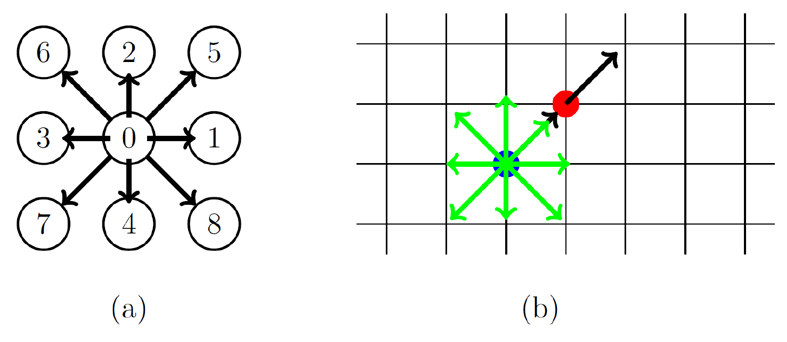
\includegraphics[width=9cm]{d2q9_scheme.png}\\
  (a) Discretization on the velocity space according to D2Q9.\\
  (b) Uniform 2D grid for the discretization in the physical space.\\
  \small{(Material from lecture)}
\end{figure}

\clearpage
\section{Milestons}
This chapter presents the results from the seven milestone and gives an in detail review.

\subsection{M1: Streaming}
As shown in equation~\ref{eq:pdf} streaming and collision are two separate terms.
The collision can be ignored by setting it to zero, i.e. $\left( \frac{\partial f}{\partial t} \right)_{col} \overset{!}{=} 0$.
This simplifies the BTE and implies the movement of particles in the vacuum with no mutual interaction between particles and is defined by equation \ref{eq:streaming}.
\begin{equation}
  \label{eq:streaming}
  \begin{aligned}
    f_{i}(r+c_{i} \nabla t,t+\nabla t)=f_{i}(r,t)
  \end{aligned}
\end{equation}
The code implementation of a streaming function on a 2D lattice is shown in listing \ref{lst:streaming}
\footnote{Throughout I will use the notation $_ixy$ where $i$ is the rolling dimension and x and y are the deminsions of the physical space.}.
\begin{center}
\begin{lstlisting}[caption=Implementation of the streaming operator,label=lst:streaming, basicstyle=\small]
def stream(f_cxy: np.array) -> np.array:
    for i in range(1, 9):
        f_cxy[i, :, :] = np.roll(f_cxy[i, :, :], 
                      shift=C_CA[i], 
                      axis=(0, 1))
    return f_cxy
  \end{lstlisting}
\end{center}
Where $f_{cxy}$ is the PDF and $C \_ CA$ are the discretized velocity directions.
For each velocity direction the streaming shifts the velocities values in the respective direction.
Testing the streaming operator can be easily done by visualizing the different shift on a 2D grid for each velocity as shown in figure \ref{fig:m1-shifting} for the velocities $v=2$ $v=3$.
\begin{figure}[ht]
\centering
\resizebox{\columnwidth}{!}{\large%% Creator: Matplotlib, PGF backend
%%
%% To include the figure in your LaTeX document, write
%%   \input{<filename>.pgf}
%%
%% Make sure the required packages are loaded in your preamble
%%   \usepackage{pgf}
%%
%% Also ensure that all the required font packages are loaded; for instance,
%% the lmodern package is sometimes necessary when using math font.
%%   \usepackage{lmodern}
%%
%% Figures using additional raster images can only be included by \input if
%% they are in the same directory as the main LaTeX file. For loading figures
%% from other directories you can use the `import` package
%%   \usepackage{import}
%%
%% and then include the figures with
%%   \import{<path to file>}{<filename>.pgf}
%%
%% Matplotlib used the following preamble
%%   \usepackage{fontspec}
%%   \setmainfont{DejaVuSerif.ttf}[Path=\detokenize{/home/joe/miniconda3/envs/high/lib/python3.9/site-packages/matplotlib/mpl-data/fonts/ttf/}]
%%   \setsansfont{DejaVuSans.ttf}[Path=\detokenize{/home/joe/miniconda3/envs/high/lib/python3.9/site-packages/matplotlib/mpl-data/fonts/ttf/}]
%%   \setmonofont{DejaVuSansMono.ttf}[Path=\detokenize{/home/joe/miniconda3/envs/high/lib/python3.9/site-packages/matplotlib/mpl-data/fonts/ttf/}]
%%
\begingroup%
\makeatletter%
\begin{pgfpicture}%
\pgfpathrectangle{\pgfpointorigin}{\pgfqpoint{15.000000in}{5.000000in}}%
\pgfusepath{use as bounding box, clip}%
\begin{pgfscope}%
\pgfsetbuttcap%
\pgfsetmiterjoin%
\pgfsetlinewidth{0.000000pt}%
\definecolor{currentstroke}{rgb}{1.000000,1.000000,1.000000}%
\pgfsetstrokecolor{currentstroke}%
\pgfsetstrokeopacity{0.000000}%
\pgfsetdash{}{0pt}%
\pgfpathmoveto{\pgfqpoint{0.000000in}{0.000000in}}%
\pgfpathlineto{\pgfqpoint{15.000000in}{0.000000in}}%
\pgfpathlineto{\pgfqpoint{15.000000in}{5.000000in}}%
\pgfpathlineto{\pgfqpoint{0.000000in}{5.000000in}}%
\pgfpathlineto{\pgfqpoint{0.000000in}{0.000000in}}%
\pgfpathclose%
\pgfusepath{}%
\end{pgfscope}%
\begin{pgfscope}%
\pgfsetbuttcap%
\pgfsetmiterjoin%
\definecolor{currentfill}{rgb}{1.000000,1.000000,1.000000}%
\pgfsetfillcolor{currentfill}%
\pgfsetlinewidth{0.000000pt}%
\definecolor{currentstroke}{rgb}{0.000000,0.000000,0.000000}%
\pgfsetstrokecolor{currentstroke}%
\pgfsetstrokeopacity{0.000000}%
\pgfsetdash{}{0pt}%
\pgfpathmoveto{\pgfqpoint{0.794097in}{3.269444in}}%
\pgfpathlineto{\pgfqpoint{3.712500in}{3.269444in}}%
\pgfpathlineto{\pgfqpoint{3.712500in}{4.850000in}}%
\pgfpathlineto{\pgfqpoint{0.794097in}{4.850000in}}%
\pgfpathlineto{\pgfqpoint{0.794097in}{3.269444in}}%
\pgfpathclose%
\pgfusepath{fill}%
\end{pgfscope}%
\begin{pgfscope}%
\pgfpathrectangle{\pgfqpoint{0.794097in}{3.269444in}}{\pgfqpoint{2.918403in}{1.580556in}}%
\pgfusepath{clip}%
\pgfsetbuttcap%
\pgfsetroundjoin%
\definecolor{currentfill}{rgb}{0.984744,0.432910,0.307420}%
\pgfsetfillcolor{currentfill}%
\pgfsetlinewidth{0.000000pt}%
\definecolor{currentstroke}{rgb}{0.000000,0.000000,0.000000}%
\pgfsetstrokecolor{currentstroke}%
\pgfsetdash{}{0pt}%
\pgfpathmoveto{\pgfqpoint{0.794097in}{3.269444in}}%
\pgfpathlineto{\pgfqpoint{0.794097in}{3.664583in}}%
\pgfpathlineto{\pgfqpoint{1.377778in}{3.664583in}}%
\pgfpathlineto{\pgfqpoint{1.377778in}{3.269444in}}%
\pgfpathlineto{\pgfqpoint{0.794097in}{3.269444in}}%
\pgfpathlineto{\pgfqpoint{0.794097in}{3.269444in}}%
\pgfpathclose%
\pgfusepath{fill}%
\end{pgfscope}%
\begin{pgfscope}%
\pgfpathrectangle{\pgfqpoint{0.794097in}{3.269444in}}{\pgfqpoint{2.918403in}{1.580556in}}%
\pgfusepath{clip}%
\pgfsetbuttcap%
\pgfsetroundjoin%
\definecolor{currentfill}{rgb}{0.974717,0.378101,0.266205}%
\pgfsetfillcolor{currentfill}%
\pgfsetlinewidth{0.000000pt}%
\definecolor{currentstroke}{rgb}{0.000000,0.000000,0.000000}%
\pgfsetstrokecolor{currentstroke}%
\pgfsetdash{}{0pt}%
\pgfpathmoveto{\pgfqpoint{1.377778in}{3.269444in}}%
\pgfpathlineto{\pgfqpoint{1.377778in}{3.664583in}}%
\pgfpathlineto{\pgfqpoint{1.961458in}{3.664583in}}%
\pgfpathlineto{\pgfqpoint{1.961458in}{3.269444in}}%
\pgfpathlineto{\pgfqpoint{1.377778in}{3.269444in}}%
\pgfpathlineto{\pgfqpoint{1.377778in}{3.269444in}}%
\pgfpathclose%
\pgfusepath{fill}%
\end{pgfscope}%
\begin{pgfscope}%
\pgfpathrectangle{\pgfqpoint{0.794097in}{3.269444in}}{\pgfqpoint{2.918403in}{1.580556in}}%
\pgfusepath{clip}%
\pgfsetbuttcap%
\pgfsetroundjoin%
\definecolor{currentfill}{rgb}{0.988235,0.681630,0.572103}%
\pgfsetfillcolor{currentfill}%
\pgfsetlinewidth{0.000000pt}%
\definecolor{currentstroke}{rgb}{0.000000,0.000000,0.000000}%
\pgfsetstrokecolor{currentstroke}%
\pgfsetdash{}{0pt}%
\pgfpathmoveto{\pgfqpoint{1.961458in}{3.269444in}}%
\pgfpathlineto{\pgfqpoint{1.961458in}{3.664583in}}%
\pgfpathlineto{\pgfqpoint{2.545139in}{3.664583in}}%
\pgfpathlineto{\pgfqpoint{2.545139in}{3.269444in}}%
\pgfpathlineto{\pgfqpoint{1.961458in}{3.269444in}}%
\pgfpathlineto{\pgfqpoint{1.961458in}{3.269444in}}%
\pgfpathclose%
\pgfusepath{fill}%
\end{pgfscope}%
\begin{pgfscope}%
\pgfpathrectangle{\pgfqpoint{0.794097in}{3.269444in}}{\pgfqpoint{2.918403in}{1.580556in}}%
\pgfusepath{clip}%
\pgfsetbuttcap%
\pgfsetroundjoin%
\definecolor{currentfill}{rgb}{0.525967,0.029527,0.066728}%
\pgfsetfillcolor{currentfill}%
\pgfsetlinewidth{0.000000pt}%
\definecolor{currentstroke}{rgb}{0.000000,0.000000,0.000000}%
\pgfsetstrokecolor{currentstroke}%
\pgfsetdash{}{0pt}%
\pgfpathmoveto{\pgfqpoint{2.545139in}{3.269444in}}%
\pgfpathlineto{\pgfqpoint{2.545139in}{3.664583in}}%
\pgfpathlineto{\pgfqpoint{3.128819in}{3.664583in}}%
\pgfpathlineto{\pgfqpoint{3.128819in}{3.269444in}}%
\pgfpathlineto{\pgfqpoint{2.545139in}{3.269444in}}%
\pgfpathlineto{\pgfqpoint{2.545139in}{3.269444in}}%
\pgfpathclose%
\pgfusepath{fill}%
\end{pgfscope}%
\begin{pgfscope}%
\pgfpathrectangle{\pgfqpoint{0.794097in}{3.269444in}}{\pgfqpoint{2.918403in}{1.580556in}}%
\pgfusepath{clip}%
\pgfsetbuttcap%
\pgfsetroundjoin%
\definecolor{currentfill}{rgb}{0.525967,0.029527,0.066728}%
\pgfsetfillcolor{currentfill}%
\pgfsetlinewidth{0.000000pt}%
\definecolor{currentstroke}{rgb}{0.000000,0.000000,0.000000}%
\pgfsetstrokecolor{currentstroke}%
\pgfsetdash{}{0pt}%
\pgfpathmoveto{\pgfqpoint{3.128819in}{3.269444in}}%
\pgfpathlineto{\pgfqpoint{3.128819in}{3.664583in}}%
\pgfpathlineto{\pgfqpoint{3.712500in}{3.664583in}}%
\pgfpathlineto{\pgfqpoint{3.712500in}{3.269444in}}%
\pgfpathlineto{\pgfqpoint{3.128819in}{3.269444in}}%
\pgfpathlineto{\pgfqpoint{3.128819in}{3.269444in}}%
\pgfpathclose%
\pgfusepath{fill}%
\end{pgfscope}%
\begin{pgfscope}%
\pgfpathrectangle{\pgfqpoint{0.794097in}{3.269444in}}{\pgfqpoint{2.918403in}{1.580556in}}%
\pgfusepath{clip}%
\pgfsetbuttcap%
\pgfsetroundjoin%
\definecolor{currentfill}{rgb}{0.974717,0.378101,0.266205}%
\pgfsetfillcolor{currentfill}%
\pgfsetlinewidth{0.000000pt}%
\definecolor{currentstroke}{rgb}{0.000000,0.000000,0.000000}%
\pgfsetstrokecolor{currentstroke}%
\pgfsetdash{}{0pt}%
\pgfpathmoveto{\pgfqpoint{0.794097in}{3.664583in}}%
\pgfpathlineto{\pgfqpoint{0.794097in}{4.059722in}}%
\pgfpathlineto{\pgfqpoint{1.377778in}{4.059722in}}%
\pgfpathlineto{\pgfqpoint{1.377778in}{3.664583in}}%
\pgfpathlineto{\pgfqpoint{0.794097in}{3.664583in}}%
\pgfpathlineto{\pgfqpoint{0.794097in}{3.664583in}}%
\pgfpathclose%
\pgfusepath{fill}%
\end{pgfscope}%
\begin{pgfscope}%
\pgfpathrectangle{\pgfqpoint{0.794097in}{3.269444in}}{\pgfqpoint{2.918403in}{1.580556in}}%
\pgfusepath{clip}%
\pgfsetbuttcap%
\pgfsetroundjoin%
\definecolor{currentfill}{rgb}{0.640384,0.057209,0.081492}%
\pgfsetfillcolor{currentfill}%
\pgfsetlinewidth{0.000000pt}%
\definecolor{currentstroke}{rgb}{0.000000,0.000000,0.000000}%
\pgfsetstrokecolor{currentstroke}%
\pgfsetdash{}{0pt}%
\pgfpathmoveto{\pgfqpoint{1.377778in}{3.664583in}}%
\pgfpathlineto{\pgfqpoint{1.377778in}{4.059722in}}%
\pgfpathlineto{\pgfqpoint{1.961458in}{4.059722in}}%
\pgfpathlineto{\pgfqpoint{1.961458in}{3.664583in}}%
\pgfpathlineto{\pgfqpoint{1.377778in}{3.664583in}}%
\pgfpathlineto{\pgfqpoint{1.377778in}{3.664583in}}%
\pgfpathclose%
\pgfusepath{fill}%
\end{pgfscope}%
\begin{pgfscope}%
\pgfpathrectangle{\pgfqpoint{0.794097in}{3.269444in}}{\pgfqpoint{2.918403in}{1.580556in}}%
\pgfusepath{clip}%
\pgfsetbuttcap%
\pgfsetroundjoin%
\definecolor{currentfill}{rgb}{0.948143,0.274018,0.199769}%
\pgfsetfillcolor{currentfill}%
\pgfsetlinewidth{0.000000pt}%
\definecolor{currentstroke}{rgb}{0.000000,0.000000,0.000000}%
\pgfsetstrokecolor{currentstroke}%
\pgfsetdash{}{0pt}%
\pgfpathmoveto{\pgfqpoint{1.961458in}{3.664583in}}%
\pgfpathlineto{\pgfqpoint{1.961458in}{4.059722in}}%
\pgfpathlineto{\pgfqpoint{2.545139in}{4.059722in}}%
\pgfpathlineto{\pgfqpoint{2.545139in}{3.664583in}}%
\pgfpathlineto{\pgfqpoint{1.961458in}{3.664583in}}%
\pgfpathlineto{\pgfqpoint{1.961458in}{3.664583in}}%
\pgfpathclose%
\pgfusepath{fill}%
\end{pgfscope}%
\begin{pgfscope}%
\pgfpathrectangle{\pgfqpoint{0.794097in}{3.269444in}}{\pgfqpoint{2.918403in}{1.580556in}}%
\pgfusepath{clip}%
\pgfsetbuttcap%
\pgfsetroundjoin%
\definecolor{currentfill}{rgb}{0.666344,0.063391,0.086413}%
\pgfsetfillcolor{currentfill}%
\pgfsetlinewidth{0.000000pt}%
\definecolor{currentstroke}{rgb}{0.000000,0.000000,0.000000}%
\pgfsetstrokecolor{currentstroke}%
\pgfsetdash{}{0pt}%
\pgfpathmoveto{\pgfqpoint{2.545139in}{3.664583in}}%
\pgfpathlineto{\pgfqpoint{2.545139in}{4.059722in}}%
\pgfpathlineto{\pgfqpoint{3.128819in}{4.059722in}}%
\pgfpathlineto{\pgfqpoint{3.128819in}{3.664583in}}%
\pgfpathlineto{\pgfqpoint{2.545139in}{3.664583in}}%
\pgfpathlineto{\pgfqpoint{2.545139in}{3.664583in}}%
\pgfpathclose%
\pgfusepath{fill}%
\end{pgfscope}%
\begin{pgfscope}%
\pgfpathrectangle{\pgfqpoint{0.794097in}{3.269444in}}{\pgfqpoint{2.918403in}{1.580556in}}%
\pgfusepath{clip}%
\pgfsetbuttcap%
\pgfsetroundjoin%
\definecolor{currentfill}{rgb}{0.988235,0.666498,0.554756}%
\pgfsetfillcolor{currentfill}%
\pgfsetlinewidth{0.000000pt}%
\definecolor{currentstroke}{rgb}{0.000000,0.000000,0.000000}%
\pgfsetstrokecolor{currentstroke}%
\pgfsetdash{}{0pt}%
\pgfpathmoveto{\pgfqpoint{3.128819in}{3.664583in}}%
\pgfpathlineto{\pgfqpoint{3.128819in}{4.059722in}}%
\pgfpathlineto{\pgfqpoint{3.712500in}{4.059722in}}%
\pgfpathlineto{\pgfqpoint{3.712500in}{3.664583in}}%
\pgfpathlineto{\pgfqpoint{3.128819in}{3.664583in}}%
\pgfpathlineto{\pgfqpoint{3.128819in}{3.664583in}}%
\pgfpathclose%
\pgfusepath{fill}%
\end{pgfscope}%
\begin{pgfscope}%
\pgfpathrectangle{\pgfqpoint{0.794097in}{3.269444in}}{\pgfqpoint{2.918403in}{1.580556in}}%
\pgfusepath{clip}%
\pgfsetbuttcap%
\pgfsetroundjoin%
\definecolor{currentfill}{rgb}{0.954048,0.297147,0.214533}%
\pgfsetfillcolor{currentfill}%
\pgfsetlinewidth{0.000000pt}%
\definecolor{currentstroke}{rgb}{0.000000,0.000000,0.000000}%
\pgfsetstrokecolor{currentstroke}%
\pgfsetdash{}{0pt}%
\pgfpathmoveto{\pgfqpoint{0.794097in}{4.059722in}}%
\pgfpathlineto{\pgfqpoint{0.794097in}{4.454861in}}%
\pgfpathlineto{\pgfqpoint{1.377778in}{4.454861in}}%
\pgfpathlineto{\pgfqpoint{1.377778in}{4.059722in}}%
\pgfpathlineto{\pgfqpoint{0.794097in}{4.059722in}}%
\pgfpathlineto{\pgfqpoint{0.794097in}{4.059722in}}%
\pgfpathclose%
\pgfusepath{fill}%
\end{pgfscope}%
\begin{pgfscope}%
\pgfpathrectangle{\pgfqpoint{0.794097in}{3.269444in}}{\pgfqpoint{2.918403in}{1.580556in}}%
\pgfusepath{clip}%
\pgfsetbuttcap%
\pgfsetroundjoin%
\definecolor{currentfill}{rgb}{0.988189,0.570704,0.445213}%
\pgfsetfillcolor{currentfill}%
\pgfsetlinewidth{0.000000pt}%
\definecolor{currentstroke}{rgb}{0.000000,0.000000,0.000000}%
\pgfsetstrokecolor{currentstroke}%
\pgfsetdash{}{0pt}%
\pgfpathmoveto{\pgfqpoint{1.377778in}{4.059722in}}%
\pgfpathlineto{\pgfqpoint{1.377778in}{4.454861in}}%
\pgfpathlineto{\pgfqpoint{1.961458in}{4.454861in}}%
\pgfpathlineto{\pgfqpoint{1.961458in}{4.059722in}}%
\pgfpathlineto{\pgfqpoint{1.377778in}{4.059722in}}%
\pgfpathlineto{\pgfqpoint{1.377778in}{4.059722in}}%
\pgfpathclose%
\pgfusepath{fill}%
\end{pgfscope}%
\begin{pgfscope}%
\pgfpathrectangle{\pgfqpoint{0.794097in}{3.269444in}}{\pgfqpoint{2.918403in}{1.580556in}}%
\pgfusepath{clip}%
\pgfsetbuttcap%
\pgfsetroundjoin%
\definecolor{currentfill}{rgb}{0.961430,0.326059,0.232987}%
\pgfsetfillcolor{currentfill}%
\pgfsetlinewidth{0.000000pt}%
\definecolor{currentstroke}{rgb}{0.000000,0.000000,0.000000}%
\pgfsetstrokecolor{currentstroke}%
\pgfsetdash{}{0pt}%
\pgfpathmoveto{\pgfqpoint{1.961458in}{4.059722in}}%
\pgfpathlineto{\pgfqpoint{1.961458in}{4.454861in}}%
\pgfpathlineto{\pgfqpoint{2.545139in}{4.454861in}}%
\pgfpathlineto{\pgfqpoint{2.545139in}{4.059722in}}%
\pgfpathlineto{\pgfqpoint{1.961458in}{4.059722in}}%
\pgfpathlineto{\pgfqpoint{1.961458in}{4.059722in}}%
\pgfpathclose%
\pgfusepath{fill}%
\end{pgfscope}%
\begin{pgfscope}%
\pgfpathrectangle{\pgfqpoint{0.794097in}{3.269444in}}{\pgfqpoint{2.918403in}{1.580556in}}%
\pgfusepath{clip}%
\pgfsetbuttcap%
\pgfsetroundjoin%
\definecolor{currentfill}{rgb}{0.990388,0.773164,0.684121}%
\pgfsetfillcolor{currentfill}%
\pgfsetlinewidth{0.000000pt}%
\definecolor{currentstroke}{rgb}{0.000000,0.000000,0.000000}%
\pgfsetstrokecolor{currentstroke}%
\pgfsetdash{}{0pt}%
\pgfpathmoveto{\pgfqpoint{2.545139in}{4.059722in}}%
\pgfpathlineto{\pgfqpoint{2.545139in}{4.454861in}}%
\pgfpathlineto{\pgfqpoint{3.128819in}{4.454861in}}%
\pgfpathlineto{\pgfqpoint{3.128819in}{4.059722in}}%
\pgfpathlineto{\pgfqpoint{2.545139in}{4.059722in}}%
\pgfpathlineto{\pgfqpoint{2.545139in}{4.059722in}}%
\pgfpathclose%
\pgfusepath{fill}%
\end{pgfscope}%
\begin{pgfscope}%
\pgfpathrectangle{\pgfqpoint{0.794097in}{3.269444in}}{\pgfqpoint{2.918403in}{1.580556in}}%
\pgfusepath{clip}%
\pgfsetbuttcap%
\pgfsetroundjoin%
\definecolor{currentfill}{rgb}{0.988235,0.575702,0.450673}%
\pgfsetfillcolor{currentfill}%
\pgfsetlinewidth{0.000000pt}%
\definecolor{currentstroke}{rgb}{0.000000,0.000000,0.000000}%
\pgfsetstrokecolor{currentstroke}%
\pgfsetdash{}{0pt}%
\pgfpathmoveto{\pgfqpoint{3.128819in}{4.059722in}}%
\pgfpathlineto{\pgfqpoint{3.128819in}{4.454861in}}%
\pgfpathlineto{\pgfqpoint{3.712500in}{4.454861in}}%
\pgfpathlineto{\pgfqpoint{3.712500in}{4.059722in}}%
\pgfpathlineto{\pgfqpoint{3.128819in}{4.059722in}}%
\pgfpathlineto{\pgfqpoint{3.128819in}{4.059722in}}%
\pgfpathclose%
\pgfusepath{fill}%
\end{pgfscope}%
\begin{pgfscope}%
\pgfpathrectangle{\pgfqpoint{0.794097in}{3.269444in}}{\pgfqpoint{2.918403in}{1.580556in}}%
\pgfusepath{clip}%
\pgfsetbuttcap%
\pgfsetroundjoin%
\definecolor{currentfill}{rgb}{0.991373,0.791373,0.708235}%
\pgfsetfillcolor{currentfill}%
\pgfsetlinewidth{0.000000pt}%
\definecolor{currentstroke}{rgb}{0.000000,0.000000,0.000000}%
\pgfsetstrokecolor{currentstroke}%
\pgfsetdash{}{0pt}%
\pgfpathmoveto{\pgfqpoint{0.794097in}{4.454861in}}%
\pgfpathlineto{\pgfqpoint{0.794097in}{4.850000in}}%
\pgfpathlineto{\pgfqpoint{1.377778in}{4.850000in}}%
\pgfpathlineto{\pgfqpoint{1.377778in}{4.454861in}}%
\pgfpathlineto{\pgfqpoint{0.794097in}{4.454861in}}%
\pgfpathlineto{\pgfqpoint{0.794097in}{4.454861in}}%
\pgfpathclose%
\pgfusepath{fill}%
\end{pgfscope}%
\begin{pgfscope}%
\pgfpathrectangle{\pgfqpoint{0.794097in}{3.269444in}}{\pgfqpoint{2.918403in}{1.580556in}}%
\pgfusepath{clip}%
\pgfsetbuttcap%
\pgfsetroundjoin%
\definecolor{currentfill}{rgb}{0.985729,0.472280,0.346790}%
\pgfsetfillcolor{currentfill}%
\pgfsetlinewidth{0.000000pt}%
\definecolor{currentstroke}{rgb}{0.000000,0.000000,0.000000}%
\pgfsetstrokecolor{currentstroke}%
\pgfsetdash{}{0pt}%
\pgfpathmoveto{\pgfqpoint{1.377778in}{4.454861in}}%
\pgfpathlineto{\pgfqpoint{1.377778in}{4.850000in}}%
\pgfpathlineto{\pgfqpoint{1.961458in}{4.850000in}}%
\pgfpathlineto{\pgfqpoint{1.961458in}{4.454861in}}%
\pgfpathlineto{\pgfqpoint{1.377778in}{4.454861in}}%
\pgfpathlineto{\pgfqpoint{1.377778in}{4.454861in}}%
\pgfpathclose%
\pgfusepath{fill}%
\end{pgfscope}%
\begin{pgfscope}%
\pgfpathrectangle{\pgfqpoint{0.794097in}{3.269444in}}{\pgfqpoint{2.918403in}{1.580556in}}%
\pgfusepath{clip}%
\pgfsetbuttcap%
\pgfsetroundjoin%
\definecolor{currentfill}{rgb}{0.868051,0.164091,0.143714}%
\pgfsetfillcolor{currentfill}%
\pgfsetlinewidth{0.000000pt}%
\definecolor{currentstroke}{rgb}{0.000000,0.000000,0.000000}%
\pgfsetstrokecolor{currentstroke}%
\pgfsetdash{}{0pt}%
\pgfpathmoveto{\pgfqpoint{1.961458in}{4.454861in}}%
\pgfpathlineto{\pgfqpoint{1.961458in}{4.850000in}}%
\pgfpathlineto{\pgfqpoint{2.545139in}{4.850000in}}%
\pgfpathlineto{\pgfqpoint{2.545139in}{4.454861in}}%
\pgfpathlineto{\pgfqpoint{1.961458in}{4.454861in}}%
\pgfpathlineto{\pgfqpoint{1.961458in}{4.454861in}}%
\pgfpathclose%
\pgfusepath{fill}%
\end{pgfscope}%
\begin{pgfscope}%
\pgfpathrectangle{\pgfqpoint{0.794097in}{3.269444in}}{\pgfqpoint{2.918403in}{1.580556in}}%
\pgfusepath{clip}%
\pgfsetbuttcap%
\pgfsetroundjoin%
\definecolor{currentfill}{rgb}{1.000000,0.960784,0.941176}%
\pgfsetfillcolor{currentfill}%
\pgfsetlinewidth{0.000000pt}%
\definecolor{currentstroke}{rgb}{0.000000,0.000000,0.000000}%
\pgfsetstrokecolor{currentstroke}%
\pgfsetdash{}{0pt}%
\pgfpathmoveto{\pgfqpoint{2.545139in}{4.454861in}}%
\pgfpathlineto{\pgfqpoint{2.545139in}{4.850000in}}%
\pgfpathlineto{\pgfqpoint{3.128819in}{4.850000in}}%
\pgfpathlineto{\pgfqpoint{3.128819in}{4.454861in}}%
\pgfpathlineto{\pgfqpoint{2.545139in}{4.454861in}}%
\pgfpathlineto{\pgfqpoint{2.545139in}{4.454861in}}%
\pgfpathclose%
\pgfusepath{fill}%
\end{pgfscope}%
\begin{pgfscope}%
\pgfpathrectangle{\pgfqpoint{0.794097in}{3.269444in}}{\pgfqpoint{2.918403in}{1.580556in}}%
\pgfusepath{clip}%
\pgfsetbuttcap%
\pgfsetroundjoin%
\definecolor{currentfill}{rgb}{0.403922,0.000000,0.050980}%
\pgfsetfillcolor{currentfill}%
\pgfsetlinewidth{0.000000pt}%
\definecolor{currentstroke}{rgb}{0.000000,0.000000,0.000000}%
\pgfsetstrokecolor{currentstroke}%
\pgfsetdash{}{0pt}%
\pgfpathmoveto{\pgfqpoint{3.128819in}{4.454861in}}%
\pgfpathlineto{\pgfqpoint{3.128819in}{4.850000in}}%
\pgfpathlineto{\pgfqpoint{3.712500in}{4.850000in}}%
\pgfpathlineto{\pgfqpoint{3.712500in}{4.454861in}}%
\pgfpathlineto{\pgfqpoint{3.128819in}{4.454861in}}%
\pgfpathlineto{\pgfqpoint{3.128819in}{4.454861in}}%
\pgfpathclose%
\pgfusepath{fill}%
\end{pgfscope}%
\begin{pgfscope}%
\pgfsetbuttcap%
\pgfsetroundjoin%
\definecolor{currentfill}{rgb}{0.000000,0.000000,0.000000}%
\pgfsetfillcolor{currentfill}%
\pgfsetlinewidth{0.803000pt}%
\definecolor{currentstroke}{rgb}{0.000000,0.000000,0.000000}%
\pgfsetstrokecolor{currentstroke}%
\pgfsetdash{}{0pt}%
\pgfsys@defobject{currentmarker}{\pgfqpoint{0.000000in}{-0.048611in}}{\pgfqpoint{0.000000in}{0.000000in}}{%
\pgfpathmoveto{\pgfqpoint{0.000000in}{0.000000in}}%
\pgfpathlineto{\pgfqpoint{0.000000in}{-0.048611in}}%
\pgfusepath{stroke,fill}%
}%
\begin{pgfscope}%
\pgfsys@transformshift{0.794097in}{3.269444in}%
\pgfsys@useobject{currentmarker}{}%
\end{pgfscope}%
\end{pgfscope}%
\begin{pgfscope}%
\definecolor{textcolor}{rgb}{0.000000,0.000000,0.000000}%
\pgfsetstrokecolor{textcolor}%
\pgfsetfillcolor{textcolor}%
\pgftext[x=0.794097in,y=3.172222in,,top]{\color{textcolor}\sffamily\fontsize{10.000000}{12.000000}\selectfont 0}%
\end{pgfscope}%
\begin{pgfscope}%
\pgfsetbuttcap%
\pgfsetroundjoin%
\definecolor{currentfill}{rgb}{0.000000,0.000000,0.000000}%
\pgfsetfillcolor{currentfill}%
\pgfsetlinewidth{0.803000pt}%
\definecolor{currentstroke}{rgb}{0.000000,0.000000,0.000000}%
\pgfsetstrokecolor{currentstroke}%
\pgfsetdash{}{0pt}%
\pgfsys@defobject{currentmarker}{\pgfqpoint{0.000000in}{-0.048611in}}{\pgfqpoint{0.000000in}{0.000000in}}{%
\pgfpathmoveto{\pgfqpoint{0.000000in}{0.000000in}}%
\pgfpathlineto{\pgfqpoint{0.000000in}{-0.048611in}}%
\pgfusepath{stroke,fill}%
}%
\begin{pgfscope}%
\pgfsys@transformshift{1.377778in}{3.269444in}%
\pgfsys@useobject{currentmarker}{}%
\end{pgfscope}%
\end{pgfscope}%
\begin{pgfscope}%
\definecolor{textcolor}{rgb}{0.000000,0.000000,0.000000}%
\pgfsetstrokecolor{textcolor}%
\pgfsetfillcolor{textcolor}%
\pgftext[x=1.377778in,y=3.172222in,,top]{\color{textcolor}\sffamily\fontsize{10.000000}{12.000000}\selectfont 1}%
\end{pgfscope}%
\begin{pgfscope}%
\pgfsetbuttcap%
\pgfsetroundjoin%
\definecolor{currentfill}{rgb}{0.000000,0.000000,0.000000}%
\pgfsetfillcolor{currentfill}%
\pgfsetlinewidth{0.803000pt}%
\definecolor{currentstroke}{rgb}{0.000000,0.000000,0.000000}%
\pgfsetstrokecolor{currentstroke}%
\pgfsetdash{}{0pt}%
\pgfsys@defobject{currentmarker}{\pgfqpoint{0.000000in}{-0.048611in}}{\pgfqpoint{0.000000in}{0.000000in}}{%
\pgfpathmoveto{\pgfqpoint{0.000000in}{0.000000in}}%
\pgfpathlineto{\pgfqpoint{0.000000in}{-0.048611in}}%
\pgfusepath{stroke,fill}%
}%
\begin{pgfscope}%
\pgfsys@transformshift{1.961458in}{3.269444in}%
\pgfsys@useobject{currentmarker}{}%
\end{pgfscope}%
\end{pgfscope}%
\begin{pgfscope}%
\definecolor{textcolor}{rgb}{0.000000,0.000000,0.000000}%
\pgfsetstrokecolor{textcolor}%
\pgfsetfillcolor{textcolor}%
\pgftext[x=1.961458in,y=3.172222in,,top]{\color{textcolor}\sffamily\fontsize{10.000000}{12.000000}\selectfont 2}%
\end{pgfscope}%
\begin{pgfscope}%
\pgfsetbuttcap%
\pgfsetroundjoin%
\definecolor{currentfill}{rgb}{0.000000,0.000000,0.000000}%
\pgfsetfillcolor{currentfill}%
\pgfsetlinewidth{0.803000pt}%
\definecolor{currentstroke}{rgb}{0.000000,0.000000,0.000000}%
\pgfsetstrokecolor{currentstroke}%
\pgfsetdash{}{0pt}%
\pgfsys@defobject{currentmarker}{\pgfqpoint{0.000000in}{-0.048611in}}{\pgfqpoint{0.000000in}{0.000000in}}{%
\pgfpathmoveto{\pgfqpoint{0.000000in}{0.000000in}}%
\pgfpathlineto{\pgfqpoint{0.000000in}{-0.048611in}}%
\pgfusepath{stroke,fill}%
}%
\begin{pgfscope}%
\pgfsys@transformshift{2.545139in}{3.269444in}%
\pgfsys@useobject{currentmarker}{}%
\end{pgfscope}%
\end{pgfscope}%
\begin{pgfscope}%
\definecolor{textcolor}{rgb}{0.000000,0.000000,0.000000}%
\pgfsetstrokecolor{textcolor}%
\pgfsetfillcolor{textcolor}%
\pgftext[x=2.545139in,y=3.172222in,,top]{\color{textcolor}\sffamily\fontsize{10.000000}{12.000000}\selectfont 3}%
\end{pgfscope}%
\begin{pgfscope}%
\pgfsetbuttcap%
\pgfsetroundjoin%
\definecolor{currentfill}{rgb}{0.000000,0.000000,0.000000}%
\pgfsetfillcolor{currentfill}%
\pgfsetlinewidth{0.803000pt}%
\definecolor{currentstroke}{rgb}{0.000000,0.000000,0.000000}%
\pgfsetstrokecolor{currentstroke}%
\pgfsetdash{}{0pt}%
\pgfsys@defobject{currentmarker}{\pgfqpoint{0.000000in}{-0.048611in}}{\pgfqpoint{0.000000in}{0.000000in}}{%
\pgfpathmoveto{\pgfqpoint{0.000000in}{0.000000in}}%
\pgfpathlineto{\pgfqpoint{0.000000in}{-0.048611in}}%
\pgfusepath{stroke,fill}%
}%
\begin{pgfscope}%
\pgfsys@transformshift{3.128819in}{3.269444in}%
\pgfsys@useobject{currentmarker}{}%
\end{pgfscope}%
\end{pgfscope}%
\begin{pgfscope}%
\definecolor{textcolor}{rgb}{0.000000,0.000000,0.000000}%
\pgfsetstrokecolor{textcolor}%
\pgfsetfillcolor{textcolor}%
\pgftext[x=3.128819in,y=3.172222in,,top]{\color{textcolor}\sffamily\fontsize{10.000000}{12.000000}\selectfont 4}%
\end{pgfscope}%
\begin{pgfscope}%
\definecolor{textcolor}{rgb}{0.000000,0.000000,0.000000}%
\pgfsetstrokecolor{textcolor}%
\pgfsetfillcolor{textcolor}%
\pgftext[x=2.253299in,y=2.982254in,,top]{\color{textcolor}\sffamily\fontsize{30.000000}{36.000000}\selectfont x axis}%
\end{pgfscope}%
\begin{pgfscope}%
\pgfsetbuttcap%
\pgfsetroundjoin%
\definecolor{currentfill}{rgb}{0.000000,0.000000,0.000000}%
\pgfsetfillcolor{currentfill}%
\pgfsetlinewidth{0.803000pt}%
\definecolor{currentstroke}{rgb}{0.000000,0.000000,0.000000}%
\pgfsetstrokecolor{currentstroke}%
\pgfsetdash{}{0pt}%
\pgfsys@defobject{currentmarker}{\pgfqpoint{-0.048611in}{0.000000in}}{\pgfqpoint{-0.000000in}{0.000000in}}{%
\pgfpathmoveto{\pgfqpoint{-0.000000in}{0.000000in}}%
\pgfpathlineto{\pgfqpoint{-0.048611in}{0.000000in}}%
\pgfusepath{stroke,fill}%
}%
\begin{pgfscope}%
\pgfsys@transformshift{0.794097in}{3.269444in}%
\pgfsys@useobject{currentmarker}{}%
\end{pgfscope}%
\end{pgfscope}%
\begin{pgfscope}%
\definecolor{textcolor}{rgb}{0.000000,0.000000,0.000000}%
\pgfsetstrokecolor{textcolor}%
\pgfsetfillcolor{textcolor}%
\pgftext[x=0.608510in, y=3.216683in, left, base]{\color{textcolor}\sffamily\fontsize{10.000000}{12.000000}\selectfont 0}%
\end{pgfscope}%
\begin{pgfscope}%
\pgfsetbuttcap%
\pgfsetroundjoin%
\definecolor{currentfill}{rgb}{0.000000,0.000000,0.000000}%
\pgfsetfillcolor{currentfill}%
\pgfsetlinewidth{0.803000pt}%
\definecolor{currentstroke}{rgb}{0.000000,0.000000,0.000000}%
\pgfsetstrokecolor{currentstroke}%
\pgfsetdash{}{0pt}%
\pgfsys@defobject{currentmarker}{\pgfqpoint{-0.048611in}{0.000000in}}{\pgfqpoint{-0.000000in}{0.000000in}}{%
\pgfpathmoveto{\pgfqpoint{-0.000000in}{0.000000in}}%
\pgfpathlineto{\pgfqpoint{-0.048611in}{0.000000in}}%
\pgfusepath{stroke,fill}%
}%
\begin{pgfscope}%
\pgfsys@transformshift{0.794097in}{3.664583in}%
\pgfsys@useobject{currentmarker}{}%
\end{pgfscope}%
\end{pgfscope}%
\begin{pgfscope}%
\definecolor{textcolor}{rgb}{0.000000,0.000000,0.000000}%
\pgfsetstrokecolor{textcolor}%
\pgfsetfillcolor{textcolor}%
\pgftext[x=0.608510in, y=3.611822in, left, base]{\color{textcolor}\sffamily\fontsize{10.000000}{12.000000}\selectfont 1}%
\end{pgfscope}%
\begin{pgfscope}%
\pgfsetbuttcap%
\pgfsetroundjoin%
\definecolor{currentfill}{rgb}{0.000000,0.000000,0.000000}%
\pgfsetfillcolor{currentfill}%
\pgfsetlinewidth{0.803000pt}%
\definecolor{currentstroke}{rgb}{0.000000,0.000000,0.000000}%
\pgfsetstrokecolor{currentstroke}%
\pgfsetdash{}{0pt}%
\pgfsys@defobject{currentmarker}{\pgfqpoint{-0.048611in}{0.000000in}}{\pgfqpoint{-0.000000in}{0.000000in}}{%
\pgfpathmoveto{\pgfqpoint{-0.000000in}{0.000000in}}%
\pgfpathlineto{\pgfqpoint{-0.048611in}{0.000000in}}%
\pgfusepath{stroke,fill}%
}%
\begin{pgfscope}%
\pgfsys@transformshift{0.794097in}{4.059722in}%
\pgfsys@useobject{currentmarker}{}%
\end{pgfscope}%
\end{pgfscope}%
\begin{pgfscope}%
\definecolor{textcolor}{rgb}{0.000000,0.000000,0.000000}%
\pgfsetstrokecolor{textcolor}%
\pgfsetfillcolor{textcolor}%
\pgftext[x=0.608510in, y=4.006961in, left, base]{\color{textcolor}\sffamily\fontsize{10.000000}{12.000000}\selectfont 2}%
\end{pgfscope}%
\begin{pgfscope}%
\pgfsetbuttcap%
\pgfsetroundjoin%
\definecolor{currentfill}{rgb}{0.000000,0.000000,0.000000}%
\pgfsetfillcolor{currentfill}%
\pgfsetlinewidth{0.803000pt}%
\definecolor{currentstroke}{rgb}{0.000000,0.000000,0.000000}%
\pgfsetstrokecolor{currentstroke}%
\pgfsetdash{}{0pt}%
\pgfsys@defobject{currentmarker}{\pgfqpoint{-0.048611in}{0.000000in}}{\pgfqpoint{-0.000000in}{0.000000in}}{%
\pgfpathmoveto{\pgfqpoint{-0.000000in}{0.000000in}}%
\pgfpathlineto{\pgfqpoint{-0.048611in}{0.000000in}}%
\pgfusepath{stroke,fill}%
}%
\begin{pgfscope}%
\pgfsys@transformshift{0.794097in}{4.454861in}%
\pgfsys@useobject{currentmarker}{}%
\end{pgfscope}%
\end{pgfscope}%
\begin{pgfscope}%
\definecolor{textcolor}{rgb}{0.000000,0.000000,0.000000}%
\pgfsetstrokecolor{textcolor}%
\pgfsetfillcolor{textcolor}%
\pgftext[x=0.608510in, y=4.402100in, left, base]{\color{textcolor}\sffamily\fontsize{10.000000}{12.000000}\selectfont 3}%
\end{pgfscope}%
\begin{pgfscope}%
\definecolor{textcolor}{rgb}{0.000000,0.000000,0.000000}%
\pgfsetstrokecolor{textcolor}%
\pgfsetfillcolor{textcolor}%
\pgftext[x=0.552954in,y=4.059722in,,bottom,rotate=90.000000]{\color{textcolor}\sffamily\fontsize{30.000000}{36.000000}\selectfont y axis}%
\end{pgfscope}%
\begin{pgfscope}%
\pgfsetrectcap%
\pgfsetmiterjoin%
\pgfsetlinewidth{0.803000pt}%
\definecolor{currentstroke}{rgb}{0.000000,0.000000,0.000000}%
\pgfsetstrokecolor{currentstroke}%
\pgfsetdash{}{0pt}%
\pgfpathmoveto{\pgfqpoint{0.794097in}{3.269444in}}%
\pgfpathlineto{\pgfqpoint{0.794097in}{4.850000in}}%
\pgfusepath{stroke}%
\end{pgfscope}%
\begin{pgfscope}%
\pgfsetrectcap%
\pgfsetmiterjoin%
\pgfsetlinewidth{0.803000pt}%
\definecolor{currentstroke}{rgb}{0.000000,0.000000,0.000000}%
\pgfsetstrokecolor{currentstroke}%
\pgfsetdash{}{0pt}%
\pgfpathmoveto{\pgfqpoint{3.712500in}{3.269444in}}%
\pgfpathlineto{\pgfqpoint{3.712500in}{4.850000in}}%
\pgfusepath{stroke}%
\end{pgfscope}%
\begin{pgfscope}%
\pgfsetrectcap%
\pgfsetmiterjoin%
\pgfsetlinewidth{0.803000pt}%
\definecolor{currentstroke}{rgb}{0.000000,0.000000,0.000000}%
\pgfsetstrokecolor{currentstroke}%
\pgfsetdash{}{0pt}%
\pgfpathmoveto{\pgfqpoint{0.794097in}{3.269444in}}%
\pgfpathlineto{\pgfqpoint{3.712500in}{3.269444in}}%
\pgfusepath{stroke}%
\end{pgfscope}%
\begin{pgfscope}%
\pgfsetrectcap%
\pgfsetmiterjoin%
\pgfsetlinewidth{0.803000pt}%
\definecolor{currentstroke}{rgb}{0.000000,0.000000,0.000000}%
\pgfsetstrokecolor{currentstroke}%
\pgfsetdash{}{0pt}%
\pgfpathmoveto{\pgfqpoint{0.794097in}{4.850000in}}%
\pgfpathlineto{\pgfqpoint{3.712500in}{4.850000in}}%
\pgfusepath{stroke}%
\end{pgfscope}%
\begin{pgfscope}%
\pgfsetbuttcap%
\pgfsetmiterjoin%
\definecolor{currentfill}{rgb}{1.000000,1.000000,1.000000}%
\pgfsetfillcolor{currentfill}%
\pgfsetlinewidth{0.000000pt}%
\definecolor{currentstroke}{rgb}{0.000000,0.000000,0.000000}%
\pgfsetstrokecolor{currentstroke}%
\pgfsetstrokeopacity{0.000000}%
\pgfsetdash{}{0pt}%
\pgfpathmoveto{\pgfqpoint{4.506597in}{3.269444in}}%
\pgfpathlineto{\pgfqpoint{7.425000in}{3.269444in}}%
\pgfpathlineto{\pgfqpoint{7.425000in}{4.850000in}}%
\pgfpathlineto{\pgfqpoint{4.506597in}{4.850000in}}%
\pgfpathlineto{\pgfqpoint{4.506597in}{3.269444in}}%
\pgfpathclose%
\pgfusepath{fill}%
\end{pgfscope}%
\begin{pgfscope}%
\pgfpathrectangle{\pgfqpoint{4.506597in}{3.269444in}}{\pgfqpoint{2.918403in}{1.580556in}}%
\pgfusepath{clip}%
\pgfsetbuttcap%
\pgfsetroundjoin%
\definecolor{currentfill}{rgb}{0.991373,0.791373,0.708235}%
\pgfsetfillcolor{currentfill}%
\pgfsetlinewidth{0.000000pt}%
\definecolor{currentstroke}{rgb}{0.000000,0.000000,0.000000}%
\pgfsetstrokecolor{currentstroke}%
\pgfsetdash{}{0pt}%
\pgfpathmoveto{\pgfqpoint{4.506597in}{3.269444in}}%
\pgfpathlineto{\pgfqpoint{4.506597in}{3.664583in}}%
\pgfpathlineto{\pgfqpoint{5.090278in}{3.664583in}}%
\pgfpathlineto{\pgfqpoint{5.090278in}{3.269444in}}%
\pgfpathlineto{\pgfqpoint{4.506597in}{3.269444in}}%
\pgfpathlineto{\pgfqpoint{4.506597in}{3.269444in}}%
\pgfpathclose%
\pgfusepath{fill}%
\end{pgfscope}%
\begin{pgfscope}%
\pgfpathrectangle{\pgfqpoint{4.506597in}{3.269444in}}{\pgfqpoint{2.918403in}{1.580556in}}%
\pgfusepath{clip}%
\pgfsetbuttcap%
\pgfsetroundjoin%
\definecolor{currentfill}{rgb}{0.985729,0.472280,0.346790}%
\pgfsetfillcolor{currentfill}%
\pgfsetlinewidth{0.000000pt}%
\definecolor{currentstroke}{rgb}{0.000000,0.000000,0.000000}%
\pgfsetstrokecolor{currentstroke}%
\pgfsetdash{}{0pt}%
\pgfpathmoveto{\pgfqpoint{5.090278in}{3.269444in}}%
\pgfpathlineto{\pgfqpoint{5.090278in}{3.664583in}}%
\pgfpathlineto{\pgfqpoint{5.673958in}{3.664583in}}%
\pgfpathlineto{\pgfqpoint{5.673958in}{3.269444in}}%
\pgfpathlineto{\pgfqpoint{5.090278in}{3.269444in}}%
\pgfpathlineto{\pgfqpoint{5.090278in}{3.269444in}}%
\pgfpathclose%
\pgfusepath{fill}%
\end{pgfscope}%
\begin{pgfscope}%
\pgfpathrectangle{\pgfqpoint{4.506597in}{3.269444in}}{\pgfqpoint{2.918403in}{1.580556in}}%
\pgfusepath{clip}%
\pgfsetbuttcap%
\pgfsetroundjoin%
\definecolor{currentfill}{rgb}{0.868051,0.164091,0.143714}%
\pgfsetfillcolor{currentfill}%
\pgfsetlinewidth{0.000000pt}%
\definecolor{currentstroke}{rgb}{0.000000,0.000000,0.000000}%
\pgfsetstrokecolor{currentstroke}%
\pgfsetdash{}{0pt}%
\pgfpathmoveto{\pgfqpoint{5.673958in}{3.269444in}}%
\pgfpathlineto{\pgfqpoint{5.673958in}{3.664583in}}%
\pgfpathlineto{\pgfqpoint{6.257639in}{3.664583in}}%
\pgfpathlineto{\pgfqpoint{6.257639in}{3.269444in}}%
\pgfpathlineto{\pgfqpoint{5.673958in}{3.269444in}}%
\pgfpathlineto{\pgfqpoint{5.673958in}{3.269444in}}%
\pgfpathclose%
\pgfusepath{fill}%
\end{pgfscope}%
\begin{pgfscope}%
\pgfpathrectangle{\pgfqpoint{4.506597in}{3.269444in}}{\pgfqpoint{2.918403in}{1.580556in}}%
\pgfusepath{clip}%
\pgfsetbuttcap%
\pgfsetroundjoin%
\definecolor{currentfill}{rgb}{1.000000,0.960784,0.941176}%
\pgfsetfillcolor{currentfill}%
\pgfsetlinewidth{0.000000pt}%
\definecolor{currentstroke}{rgb}{0.000000,0.000000,0.000000}%
\pgfsetstrokecolor{currentstroke}%
\pgfsetdash{}{0pt}%
\pgfpathmoveto{\pgfqpoint{6.257639in}{3.269444in}}%
\pgfpathlineto{\pgfqpoint{6.257639in}{3.664583in}}%
\pgfpathlineto{\pgfqpoint{6.841319in}{3.664583in}}%
\pgfpathlineto{\pgfqpoint{6.841319in}{3.269444in}}%
\pgfpathlineto{\pgfqpoint{6.257639in}{3.269444in}}%
\pgfpathlineto{\pgfqpoint{6.257639in}{3.269444in}}%
\pgfpathclose%
\pgfusepath{fill}%
\end{pgfscope}%
\begin{pgfscope}%
\pgfpathrectangle{\pgfqpoint{4.506597in}{3.269444in}}{\pgfqpoint{2.918403in}{1.580556in}}%
\pgfusepath{clip}%
\pgfsetbuttcap%
\pgfsetroundjoin%
\definecolor{currentfill}{rgb}{0.403922,0.000000,0.050980}%
\pgfsetfillcolor{currentfill}%
\pgfsetlinewidth{0.000000pt}%
\definecolor{currentstroke}{rgb}{0.000000,0.000000,0.000000}%
\pgfsetstrokecolor{currentstroke}%
\pgfsetdash{}{0pt}%
\pgfpathmoveto{\pgfqpoint{6.841319in}{3.269444in}}%
\pgfpathlineto{\pgfqpoint{6.841319in}{3.664583in}}%
\pgfpathlineto{\pgfqpoint{7.425000in}{3.664583in}}%
\pgfpathlineto{\pgfqpoint{7.425000in}{3.269444in}}%
\pgfpathlineto{\pgfqpoint{6.841319in}{3.269444in}}%
\pgfpathlineto{\pgfqpoint{6.841319in}{3.269444in}}%
\pgfpathclose%
\pgfusepath{fill}%
\end{pgfscope}%
\begin{pgfscope}%
\pgfpathrectangle{\pgfqpoint{4.506597in}{3.269444in}}{\pgfqpoint{2.918403in}{1.580556in}}%
\pgfusepath{clip}%
\pgfsetbuttcap%
\pgfsetroundjoin%
\definecolor{currentfill}{rgb}{0.984744,0.432910,0.307420}%
\pgfsetfillcolor{currentfill}%
\pgfsetlinewidth{0.000000pt}%
\definecolor{currentstroke}{rgb}{0.000000,0.000000,0.000000}%
\pgfsetstrokecolor{currentstroke}%
\pgfsetdash{}{0pt}%
\pgfpathmoveto{\pgfqpoint{4.506597in}{3.664583in}}%
\pgfpathlineto{\pgfqpoint{4.506597in}{4.059722in}}%
\pgfpathlineto{\pgfqpoint{5.090278in}{4.059722in}}%
\pgfpathlineto{\pgfqpoint{5.090278in}{3.664583in}}%
\pgfpathlineto{\pgfqpoint{4.506597in}{3.664583in}}%
\pgfpathlineto{\pgfqpoint{4.506597in}{3.664583in}}%
\pgfpathclose%
\pgfusepath{fill}%
\end{pgfscope}%
\begin{pgfscope}%
\pgfpathrectangle{\pgfqpoint{4.506597in}{3.269444in}}{\pgfqpoint{2.918403in}{1.580556in}}%
\pgfusepath{clip}%
\pgfsetbuttcap%
\pgfsetroundjoin%
\definecolor{currentfill}{rgb}{0.974717,0.378101,0.266205}%
\pgfsetfillcolor{currentfill}%
\pgfsetlinewidth{0.000000pt}%
\definecolor{currentstroke}{rgb}{0.000000,0.000000,0.000000}%
\pgfsetstrokecolor{currentstroke}%
\pgfsetdash{}{0pt}%
\pgfpathmoveto{\pgfqpoint{5.090278in}{3.664583in}}%
\pgfpathlineto{\pgfqpoint{5.090278in}{4.059722in}}%
\pgfpathlineto{\pgfqpoint{5.673958in}{4.059722in}}%
\pgfpathlineto{\pgfqpoint{5.673958in}{3.664583in}}%
\pgfpathlineto{\pgfqpoint{5.090278in}{3.664583in}}%
\pgfpathlineto{\pgfqpoint{5.090278in}{3.664583in}}%
\pgfpathclose%
\pgfusepath{fill}%
\end{pgfscope}%
\begin{pgfscope}%
\pgfpathrectangle{\pgfqpoint{4.506597in}{3.269444in}}{\pgfqpoint{2.918403in}{1.580556in}}%
\pgfusepath{clip}%
\pgfsetbuttcap%
\pgfsetroundjoin%
\definecolor{currentfill}{rgb}{0.988235,0.681630,0.572103}%
\pgfsetfillcolor{currentfill}%
\pgfsetlinewidth{0.000000pt}%
\definecolor{currentstroke}{rgb}{0.000000,0.000000,0.000000}%
\pgfsetstrokecolor{currentstroke}%
\pgfsetdash{}{0pt}%
\pgfpathmoveto{\pgfqpoint{5.673958in}{3.664583in}}%
\pgfpathlineto{\pgfqpoint{5.673958in}{4.059722in}}%
\pgfpathlineto{\pgfqpoint{6.257639in}{4.059722in}}%
\pgfpathlineto{\pgfqpoint{6.257639in}{3.664583in}}%
\pgfpathlineto{\pgfqpoint{5.673958in}{3.664583in}}%
\pgfpathlineto{\pgfqpoint{5.673958in}{3.664583in}}%
\pgfpathclose%
\pgfusepath{fill}%
\end{pgfscope}%
\begin{pgfscope}%
\pgfpathrectangle{\pgfqpoint{4.506597in}{3.269444in}}{\pgfqpoint{2.918403in}{1.580556in}}%
\pgfusepath{clip}%
\pgfsetbuttcap%
\pgfsetroundjoin%
\definecolor{currentfill}{rgb}{0.525967,0.029527,0.066728}%
\pgfsetfillcolor{currentfill}%
\pgfsetlinewidth{0.000000pt}%
\definecolor{currentstroke}{rgb}{0.000000,0.000000,0.000000}%
\pgfsetstrokecolor{currentstroke}%
\pgfsetdash{}{0pt}%
\pgfpathmoveto{\pgfqpoint{6.257639in}{3.664583in}}%
\pgfpathlineto{\pgfqpoint{6.257639in}{4.059722in}}%
\pgfpathlineto{\pgfqpoint{6.841319in}{4.059722in}}%
\pgfpathlineto{\pgfqpoint{6.841319in}{3.664583in}}%
\pgfpathlineto{\pgfqpoint{6.257639in}{3.664583in}}%
\pgfpathlineto{\pgfqpoint{6.257639in}{3.664583in}}%
\pgfpathclose%
\pgfusepath{fill}%
\end{pgfscope}%
\begin{pgfscope}%
\pgfpathrectangle{\pgfqpoint{4.506597in}{3.269444in}}{\pgfqpoint{2.918403in}{1.580556in}}%
\pgfusepath{clip}%
\pgfsetbuttcap%
\pgfsetroundjoin%
\definecolor{currentfill}{rgb}{0.525967,0.029527,0.066728}%
\pgfsetfillcolor{currentfill}%
\pgfsetlinewidth{0.000000pt}%
\definecolor{currentstroke}{rgb}{0.000000,0.000000,0.000000}%
\pgfsetstrokecolor{currentstroke}%
\pgfsetdash{}{0pt}%
\pgfpathmoveto{\pgfqpoint{6.841319in}{3.664583in}}%
\pgfpathlineto{\pgfqpoint{6.841319in}{4.059722in}}%
\pgfpathlineto{\pgfqpoint{7.425000in}{4.059722in}}%
\pgfpathlineto{\pgfqpoint{7.425000in}{3.664583in}}%
\pgfpathlineto{\pgfqpoint{6.841319in}{3.664583in}}%
\pgfpathlineto{\pgfqpoint{6.841319in}{3.664583in}}%
\pgfpathclose%
\pgfusepath{fill}%
\end{pgfscope}%
\begin{pgfscope}%
\pgfpathrectangle{\pgfqpoint{4.506597in}{3.269444in}}{\pgfqpoint{2.918403in}{1.580556in}}%
\pgfusepath{clip}%
\pgfsetbuttcap%
\pgfsetroundjoin%
\definecolor{currentfill}{rgb}{0.974717,0.378101,0.266205}%
\pgfsetfillcolor{currentfill}%
\pgfsetlinewidth{0.000000pt}%
\definecolor{currentstroke}{rgb}{0.000000,0.000000,0.000000}%
\pgfsetstrokecolor{currentstroke}%
\pgfsetdash{}{0pt}%
\pgfpathmoveto{\pgfqpoint{4.506597in}{4.059722in}}%
\pgfpathlineto{\pgfqpoint{4.506597in}{4.454861in}}%
\pgfpathlineto{\pgfqpoint{5.090278in}{4.454861in}}%
\pgfpathlineto{\pgfqpoint{5.090278in}{4.059722in}}%
\pgfpathlineto{\pgfqpoint{4.506597in}{4.059722in}}%
\pgfpathlineto{\pgfqpoint{4.506597in}{4.059722in}}%
\pgfpathclose%
\pgfusepath{fill}%
\end{pgfscope}%
\begin{pgfscope}%
\pgfpathrectangle{\pgfqpoint{4.506597in}{3.269444in}}{\pgfqpoint{2.918403in}{1.580556in}}%
\pgfusepath{clip}%
\pgfsetbuttcap%
\pgfsetroundjoin%
\definecolor{currentfill}{rgb}{0.640384,0.057209,0.081492}%
\pgfsetfillcolor{currentfill}%
\pgfsetlinewidth{0.000000pt}%
\definecolor{currentstroke}{rgb}{0.000000,0.000000,0.000000}%
\pgfsetstrokecolor{currentstroke}%
\pgfsetdash{}{0pt}%
\pgfpathmoveto{\pgfqpoint{5.090278in}{4.059722in}}%
\pgfpathlineto{\pgfqpoint{5.090278in}{4.454861in}}%
\pgfpathlineto{\pgfqpoint{5.673958in}{4.454861in}}%
\pgfpathlineto{\pgfqpoint{5.673958in}{4.059722in}}%
\pgfpathlineto{\pgfqpoint{5.090278in}{4.059722in}}%
\pgfpathlineto{\pgfqpoint{5.090278in}{4.059722in}}%
\pgfpathclose%
\pgfusepath{fill}%
\end{pgfscope}%
\begin{pgfscope}%
\pgfpathrectangle{\pgfqpoint{4.506597in}{3.269444in}}{\pgfqpoint{2.918403in}{1.580556in}}%
\pgfusepath{clip}%
\pgfsetbuttcap%
\pgfsetroundjoin%
\definecolor{currentfill}{rgb}{0.948143,0.274018,0.199769}%
\pgfsetfillcolor{currentfill}%
\pgfsetlinewidth{0.000000pt}%
\definecolor{currentstroke}{rgb}{0.000000,0.000000,0.000000}%
\pgfsetstrokecolor{currentstroke}%
\pgfsetdash{}{0pt}%
\pgfpathmoveto{\pgfqpoint{5.673958in}{4.059722in}}%
\pgfpathlineto{\pgfqpoint{5.673958in}{4.454861in}}%
\pgfpathlineto{\pgfqpoint{6.257639in}{4.454861in}}%
\pgfpathlineto{\pgfqpoint{6.257639in}{4.059722in}}%
\pgfpathlineto{\pgfqpoint{5.673958in}{4.059722in}}%
\pgfpathlineto{\pgfqpoint{5.673958in}{4.059722in}}%
\pgfpathclose%
\pgfusepath{fill}%
\end{pgfscope}%
\begin{pgfscope}%
\pgfpathrectangle{\pgfqpoint{4.506597in}{3.269444in}}{\pgfqpoint{2.918403in}{1.580556in}}%
\pgfusepath{clip}%
\pgfsetbuttcap%
\pgfsetroundjoin%
\definecolor{currentfill}{rgb}{0.666344,0.063391,0.086413}%
\pgfsetfillcolor{currentfill}%
\pgfsetlinewidth{0.000000pt}%
\definecolor{currentstroke}{rgb}{0.000000,0.000000,0.000000}%
\pgfsetstrokecolor{currentstroke}%
\pgfsetdash{}{0pt}%
\pgfpathmoveto{\pgfqpoint{6.257639in}{4.059722in}}%
\pgfpathlineto{\pgfqpoint{6.257639in}{4.454861in}}%
\pgfpathlineto{\pgfqpoint{6.841319in}{4.454861in}}%
\pgfpathlineto{\pgfqpoint{6.841319in}{4.059722in}}%
\pgfpathlineto{\pgfqpoint{6.257639in}{4.059722in}}%
\pgfpathlineto{\pgfqpoint{6.257639in}{4.059722in}}%
\pgfpathclose%
\pgfusepath{fill}%
\end{pgfscope}%
\begin{pgfscope}%
\pgfpathrectangle{\pgfqpoint{4.506597in}{3.269444in}}{\pgfqpoint{2.918403in}{1.580556in}}%
\pgfusepath{clip}%
\pgfsetbuttcap%
\pgfsetroundjoin%
\definecolor{currentfill}{rgb}{0.988235,0.666498,0.554756}%
\pgfsetfillcolor{currentfill}%
\pgfsetlinewidth{0.000000pt}%
\definecolor{currentstroke}{rgb}{0.000000,0.000000,0.000000}%
\pgfsetstrokecolor{currentstroke}%
\pgfsetdash{}{0pt}%
\pgfpathmoveto{\pgfqpoint{6.841319in}{4.059722in}}%
\pgfpathlineto{\pgfqpoint{6.841319in}{4.454861in}}%
\pgfpathlineto{\pgfqpoint{7.425000in}{4.454861in}}%
\pgfpathlineto{\pgfqpoint{7.425000in}{4.059722in}}%
\pgfpathlineto{\pgfqpoint{6.841319in}{4.059722in}}%
\pgfpathlineto{\pgfqpoint{6.841319in}{4.059722in}}%
\pgfpathclose%
\pgfusepath{fill}%
\end{pgfscope}%
\begin{pgfscope}%
\pgfpathrectangle{\pgfqpoint{4.506597in}{3.269444in}}{\pgfqpoint{2.918403in}{1.580556in}}%
\pgfusepath{clip}%
\pgfsetbuttcap%
\pgfsetroundjoin%
\definecolor{currentfill}{rgb}{0.954048,0.297147,0.214533}%
\pgfsetfillcolor{currentfill}%
\pgfsetlinewidth{0.000000pt}%
\definecolor{currentstroke}{rgb}{0.000000,0.000000,0.000000}%
\pgfsetstrokecolor{currentstroke}%
\pgfsetdash{}{0pt}%
\pgfpathmoveto{\pgfqpoint{4.506597in}{4.454861in}}%
\pgfpathlineto{\pgfqpoint{4.506597in}{4.850000in}}%
\pgfpathlineto{\pgfqpoint{5.090278in}{4.850000in}}%
\pgfpathlineto{\pgfqpoint{5.090278in}{4.454861in}}%
\pgfpathlineto{\pgfqpoint{4.506597in}{4.454861in}}%
\pgfpathlineto{\pgfqpoint{4.506597in}{4.454861in}}%
\pgfpathclose%
\pgfusepath{fill}%
\end{pgfscope}%
\begin{pgfscope}%
\pgfpathrectangle{\pgfqpoint{4.506597in}{3.269444in}}{\pgfqpoint{2.918403in}{1.580556in}}%
\pgfusepath{clip}%
\pgfsetbuttcap%
\pgfsetroundjoin%
\definecolor{currentfill}{rgb}{0.988189,0.570704,0.445213}%
\pgfsetfillcolor{currentfill}%
\pgfsetlinewidth{0.000000pt}%
\definecolor{currentstroke}{rgb}{0.000000,0.000000,0.000000}%
\pgfsetstrokecolor{currentstroke}%
\pgfsetdash{}{0pt}%
\pgfpathmoveto{\pgfqpoint{5.090278in}{4.454861in}}%
\pgfpathlineto{\pgfqpoint{5.090278in}{4.850000in}}%
\pgfpathlineto{\pgfqpoint{5.673958in}{4.850000in}}%
\pgfpathlineto{\pgfqpoint{5.673958in}{4.454861in}}%
\pgfpathlineto{\pgfqpoint{5.090278in}{4.454861in}}%
\pgfpathlineto{\pgfqpoint{5.090278in}{4.454861in}}%
\pgfpathclose%
\pgfusepath{fill}%
\end{pgfscope}%
\begin{pgfscope}%
\pgfpathrectangle{\pgfqpoint{4.506597in}{3.269444in}}{\pgfqpoint{2.918403in}{1.580556in}}%
\pgfusepath{clip}%
\pgfsetbuttcap%
\pgfsetroundjoin%
\definecolor{currentfill}{rgb}{0.961430,0.326059,0.232987}%
\pgfsetfillcolor{currentfill}%
\pgfsetlinewidth{0.000000pt}%
\definecolor{currentstroke}{rgb}{0.000000,0.000000,0.000000}%
\pgfsetstrokecolor{currentstroke}%
\pgfsetdash{}{0pt}%
\pgfpathmoveto{\pgfqpoint{5.673958in}{4.454861in}}%
\pgfpathlineto{\pgfqpoint{5.673958in}{4.850000in}}%
\pgfpathlineto{\pgfqpoint{6.257639in}{4.850000in}}%
\pgfpathlineto{\pgfqpoint{6.257639in}{4.454861in}}%
\pgfpathlineto{\pgfqpoint{5.673958in}{4.454861in}}%
\pgfpathlineto{\pgfqpoint{5.673958in}{4.454861in}}%
\pgfpathclose%
\pgfusepath{fill}%
\end{pgfscope}%
\begin{pgfscope}%
\pgfpathrectangle{\pgfqpoint{4.506597in}{3.269444in}}{\pgfqpoint{2.918403in}{1.580556in}}%
\pgfusepath{clip}%
\pgfsetbuttcap%
\pgfsetroundjoin%
\definecolor{currentfill}{rgb}{0.990388,0.773164,0.684121}%
\pgfsetfillcolor{currentfill}%
\pgfsetlinewidth{0.000000pt}%
\definecolor{currentstroke}{rgb}{0.000000,0.000000,0.000000}%
\pgfsetstrokecolor{currentstroke}%
\pgfsetdash{}{0pt}%
\pgfpathmoveto{\pgfqpoint{6.257639in}{4.454861in}}%
\pgfpathlineto{\pgfqpoint{6.257639in}{4.850000in}}%
\pgfpathlineto{\pgfqpoint{6.841319in}{4.850000in}}%
\pgfpathlineto{\pgfqpoint{6.841319in}{4.454861in}}%
\pgfpathlineto{\pgfqpoint{6.257639in}{4.454861in}}%
\pgfpathlineto{\pgfqpoint{6.257639in}{4.454861in}}%
\pgfpathclose%
\pgfusepath{fill}%
\end{pgfscope}%
\begin{pgfscope}%
\pgfpathrectangle{\pgfqpoint{4.506597in}{3.269444in}}{\pgfqpoint{2.918403in}{1.580556in}}%
\pgfusepath{clip}%
\pgfsetbuttcap%
\pgfsetroundjoin%
\definecolor{currentfill}{rgb}{0.988235,0.575702,0.450673}%
\pgfsetfillcolor{currentfill}%
\pgfsetlinewidth{0.000000pt}%
\definecolor{currentstroke}{rgb}{0.000000,0.000000,0.000000}%
\pgfsetstrokecolor{currentstroke}%
\pgfsetdash{}{0pt}%
\pgfpathmoveto{\pgfqpoint{6.841319in}{4.454861in}}%
\pgfpathlineto{\pgfqpoint{6.841319in}{4.850000in}}%
\pgfpathlineto{\pgfqpoint{7.425000in}{4.850000in}}%
\pgfpathlineto{\pgfqpoint{7.425000in}{4.454861in}}%
\pgfpathlineto{\pgfqpoint{6.841319in}{4.454861in}}%
\pgfpathlineto{\pgfqpoint{6.841319in}{4.454861in}}%
\pgfpathclose%
\pgfusepath{fill}%
\end{pgfscope}%
\begin{pgfscope}%
\pgfsetbuttcap%
\pgfsetroundjoin%
\definecolor{currentfill}{rgb}{0.000000,0.000000,0.000000}%
\pgfsetfillcolor{currentfill}%
\pgfsetlinewidth{0.803000pt}%
\definecolor{currentstroke}{rgb}{0.000000,0.000000,0.000000}%
\pgfsetstrokecolor{currentstroke}%
\pgfsetdash{}{0pt}%
\pgfsys@defobject{currentmarker}{\pgfqpoint{0.000000in}{-0.048611in}}{\pgfqpoint{0.000000in}{0.000000in}}{%
\pgfpathmoveto{\pgfqpoint{0.000000in}{0.000000in}}%
\pgfpathlineto{\pgfqpoint{0.000000in}{-0.048611in}}%
\pgfusepath{stroke,fill}%
}%
\begin{pgfscope}%
\pgfsys@transformshift{4.506597in}{3.269444in}%
\pgfsys@useobject{currentmarker}{}%
\end{pgfscope}%
\end{pgfscope}%
\begin{pgfscope}%
\definecolor{textcolor}{rgb}{0.000000,0.000000,0.000000}%
\pgfsetstrokecolor{textcolor}%
\pgfsetfillcolor{textcolor}%
\pgftext[x=4.506597in,y=3.172222in,,top]{\color{textcolor}\sffamily\fontsize{10.000000}{12.000000}\selectfont 0}%
\end{pgfscope}%
\begin{pgfscope}%
\pgfsetbuttcap%
\pgfsetroundjoin%
\definecolor{currentfill}{rgb}{0.000000,0.000000,0.000000}%
\pgfsetfillcolor{currentfill}%
\pgfsetlinewidth{0.803000pt}%
\definecolor{currentstroke}{rgb}{0.000000,0.000000,0.000000}%
\pgfsetstrokecolor{currentstroke}%
\pgfsetdash{}{0pt}%
\pgfsys@defobject{currentmarker}{\pgfqpoint{0.000000in}{-0.048611in}}{\pgfqpoint{0.000000in}{0.000000in}}{%
\pgfpathmoveto{\pgfqpoint{0.000000in}{0.000000in}}%
\pgfpathlineto{\pgfqpoint{0.000000in}{-0.048611in}}%
\pgfusepath{stroke,fill}%
}%
\begin{pgfscope}%
\pgfsys@transformshift{5.090278in}{3.269444in}%
\pgfsys@useobject{currentmarker}{}%
\end{pgfscope}%
\end{pgfscope}%
\begin{pgfscope}%
\definecolor{textcolor}{rgb}{0.000000,0.000000,0.000000}%
\pgfsetstrokecolor{textcolor}%
\pgfsetfillcolor{textcolor}%
\pgftext[x=5.090278in,y=3.172222in,,top]{\color{textcolor}\sffamily\fontsize{10.000000}{12.000000}\selectfont 1}%
\end{pgfscope}%
\begin{pgfscope}%
\pgfsetbuttcap%
\pgfsetroundjoin%
\definecolor{currentfill}{rgb}{0.000000,0.000000,0.000000}%
\pgfsetfillcolor{currentfill}%
\pgfsetlinewidth{0.803000pt}%
\definecolor{currentstroke}{rgb}{0.000000,0.000000,0.000000}%
\pgfsetstrokecolor{currentstroke}%
\pgfsetdash{}{0pt}%
\pgfsys@defobject{currentmarker}{\pgfqpoint{0.000000in}{-0.048611in}}{\pgfqpoint{0.000000in}{0.000000in}}{%
\pgfpathmoveto{\pgfqpoint{0.000000in}{0.000000in}}%
\pgfpathlineto{\pgfqpoint{0.000000in}{-0.048611in}}%
\pgfusepath{stroke,fill}%
}%
\begin{pgfscope}%
\pgfsys@transformshift{5.673958in}{3.269444in}%
\pgfsys@useobject{currentmarker}{}%
\end{pgfscope}%
\end{pgfscope}%
\begin{pgfscope}%
\definecolor{textcolor}{rgb}{0.000000,0.000000,0.000000}%
\pgfsetstrokecolor{textcolor}%
\pgfsetfillcolor{textcolor}%
\pgftext[x=5.673958in,y=3.172222in,,top]{\color{textcolor}\sffamily\fontsize{10.000000}{12.000000}\selectfont 2}%
\end{pgfscope}%
\begin{pgfscope}%
\pgfsetbuttcap%
\pgfsetroundjoin%
\definecolor{currentfill}{rgb}{0.000000,0.000000,0.000000}%
\pgfsetfillcolor{currentfill}%
\pgfsetlinewidth{0.803000pt}%
\definecolor{currentstroke}{rgb}{0.000000,0.000000,0.000000}%
\pgfsetstrokecolor{currentstroke}%
\pgfsetdash{}{0pt}%
\pgfsys@defobject{currentmarker}{\pgfqpoint{0.000000in}{-0.048611in}}{\pgfqpoint{0.000000in}{0.000000in}}{%
\pgfpathmoveto{\pgfqpoint{0.000000in}{0.000000in}}%
\pgfpathlineto{\pgfqpoint{0.000000in}{-0.048611in}}%
\pgfusepath{stroke,fill}%
}%
\begin{pgfscope}%
\pgfsys@transformshift{6.257639in}{3.269444in}%
\pgfsys@useobject{currentmarker}{}%
\end{pgfscope}%
\end{pgfscope}%
\begin{pgfscope}%
\definecolor{textcolor}{rgb}{0.000000,0.000000,0.000000}%
\pgfsetstrokecolor{textcolor}%
\pgfsetfillcolor{textcolor}%
\pgftext[x=6.257639in,y=3.172222in,,top]{\color{textcolor}\sffamily\fontsize{10.000000}{12.000000}\selectfont 3}%
\end{pgfscope}%
\begin{pgfscope}%
\pgfsetbuttcap%
\pgfsetroundjoin%
\definecolor{currentfill}{rgb}{0.000000,0.000000,0.000000}%
\pgfsetfillcolor{currentfill}%
\pgfsetlinewidth{0.803000pt}%
\definecolor{currentstroke}{rgb}{0.000000,0.000000,0.000000}%
\pgfsetstrokecolor{currentstroke}%
\pgfsetdash{}{0pt}%
\pgfsys@defobject{currentmarker}{\pgfqpoint{0.000000in}{-0.048611in}}{\pgfqpoint{0.000000in}{0.000000in}}{%
\pgfpathmoveto{\pgfqpoint{0.000000in}{0.000000in}}%
\pgfpathlineto{\pgfqpoint{0.000000in}{-0.048611in}}%
\pgfusepath{stroke,fill}%
}%
\begin{pgfscope}%
\pgfsys@transformshift{6.841319in}{3.269444in}%
\pgfsys@useobject{currentmarker}{}%
\end{pgfscope}%
\end{pgfscope}%
\begin{pgfscope}%
\definecolor{textcolor}{rgb}{0.000000,0.000000,0.000000}%
\pgfsetstrokecolor{textcolor}%
\pgfsetfillcolor{textcolor}%
\pgftext[x=6.841319in,y=3.172222in,,top]{\color{textcolor}\sffamily\fontsize{10.000000}{12.000000}\selectfont 4}%
\end{pgfscope}%
\begin{pgfscope}%
\definecolor{textcolor}{rgb}{0.000000,0.000000,0.000000}%
\pgfsetstrokecolor{textcolor}%
\pgfsetfillcolor{textcolor}%
\pgftext[x=5.965799in,y=2.982254in,,top]{\color{textcolor}\sffamily\fontsize{30.000000}{36.000000}\selectfont x axis}%
\end{pgfscope}%
\begin{pgfscope}%
\pgfsetbuttcap%
\pgfsetroundjoin%
\definecolor{currentfill}{rgb}{0.000000,0.000000,0.000000}%
\pgfsetfillcolor{currentfill}%
\pgfsetlinewidth{0.803000pt}%
\definecolor{currentstroke}{rgb}{0.000000,0.000000,0.000000}%
\pgfsetstrokecolor{currentstroke}%
\pgfsetdash{}{0pt}%
\pgfsys@defobject{currentmarker}{\pgfqpoint{-0.048611in}{0.000000in}}{\pgfqpoint{-0.000000in}{0.000000in}}{%
\pgfpathmoveto{\pgfqpoint{-0.000000in}{0.000000in}}%
\pgfpathlineto{\pgfqpoint{-0.048611in}{0.000000in}}%
\pgfusepath{stroke,fill}%
}%
\begin{pgfscope}%
\pgfsys@transformshift{4.506597in}{3.269444in}%
\pgfsys@useobject{currentmarker}{}%
\end{pgfscope}%
\end{pgfscope}%
\begin{pgfscope}%
\definecolor{textcolor}{rgb}{0.000000,0.000000,0.000000}%
\pgfsetstrokecolor{textcolor}%
\pgfsetfillcolor{textcolor}%
\pgftext[x=4.321010in, y=3.216683in, left, base]{\color{textcolor}\sffamily\fontsize{10.000000}{12.000000}\selectfont 0}%
\end{pgfscope}%
\begin{pgfscope}%
\pgfsetbuttcap%
\pgfsetroundjoin%
\definecolor{currentfill}{rgb}{0.000000,0.000000,0.000000}%
\pgfsetfillcolor{currentfill}%
\pgfsetlinewidth{0.803000pt}%
\definecolor{currentstroke}{rgb}{0.000000,0.000000,0.000000}%
\pgfsetstrokecolor{currentstroke}%
\pgfsetdash{}{0pt}%
\pgfsys@defobject{currentmarker}{\pgfqpoint{-0.048611in}{0.000000in}}{\pgfqpoint{-0.000000in}{0.000000in}}{%
\pgfpathmoveto{\pgfqpoint{-0.000000in}{0.000000in}}%
\pgfpathlineto{\pgfqpoint{-0.048611in}{0.000000in}}%
\pgfusepath{stroke,fill}%
}%
\begin{pgfscope}%
\pgfsys@transformshift{4.506597in}{3.664583in}%
\pgfsys@useobject{currentmarker}{}%
\end{pgfscope}%
\end{pgfscope}%
\begin{pgfscope}%
\definecolor{textcolor}{rgb}{0.000000,0.000000,0.000000}%
\pgfsetstrokecolor{textcolor}%
\pgfsetfillcolor{textcolor}%
\pgftext[x=4.321010in, y=3.611822in, left, base]{\color{textcolor}\sffamily\fontsize{10.000000}{12.000000}\selectfont 1}%
\end{pgfscope}%
\begin{pgfscope}%
\pgfsetbuttcap%
\pgfsetroundjoin%
\definecolor{currentfill}{rgb}{0.000000,0.000000,0.000000}%
\pgfsetfillcolor{currentfill}%
\pgfsetlinewidth{0.803000pt}%
\definecolor{currentstroke}{rgb}{0.000000,0.000000,0.000000}%
\pgfsetstrokecolor{currentstroke}%
\pgfsetdash{}{0pt}%
\pgfsys@defobject{currentmarker}{\pgfqpoint{-0.048611in}{0.000000in}}{\pgfqpoint{-0.000000in}{0.000000in}}{%
\pgfpathmoveto{\pgfqpoint{-0.000000in}{0.000000in}}%
\pgfpathlineto{\pgfqpoint{-0.048611in}{0.000000in}}%
\pgfusepath{stroke,fill}%
}%
\begin{pgfscope}%
\pgfsys@transformshift{4.506597in}{4.059722in}%
\pgfsys@useobject{currentmarker}{}%
\end{pgfscope}%
\end{pgfscope}%
\begin{pgfscope}%
\definecolor{textcolor}{rgb}{0.000000,0.000000,0.000000}%
\pgfsetstrokecolor{textcolor}%
\pgfsetfillcolor{textcolor}%
\pgftext[x=4.321010in, y=4.006961in, left, base]{\color{textcolor}\sffamily\fontsize{10.000000}{12.000000}\selectfont 2}%
\end{pgfscope}%
\begin{pgfscope}%
\pgfsetbuttcap%
\pgfsetroundjoin%
\definecolor{currentfill}{rgb}{0.000000,0.000000,0.000000}%
\pgfsetfillcolor{currentfill}%
\pgfsetlinewidth{0.803000pt}%
\definecolor{currentstroke}{rgb}{0.000000,0.000000,0.000000}%
\pgfsetstrokecolor{currentstroke}%
\pgfsetdash{}{0pt}%
\pgfsys@defobject{currentmarker}{\pgfqpoint{-0.048611in}{0.000000in}}{\pgfqpoint{-0.000000in}{0.000000in}}{%
\pgfpathmoveto{\pgfqpoint{-0.000000in}{0.000000in}}%
\pgfpathlineto{\pgfqpoint{-0.048611in}{0.000000in}}%
\pgfusepath{stroke,fill}%
}%
\begin{pgfscope}%
\pgfsys@transformshift{4.506597in}{4.454861in}%
\pgfsys@useobject{currentmarker}{}%
\end{pgfscope}%
\end{pgfscope}%
\begin{pgfscope}%
\definecolor{textcolor}{rgb}{0.000000,0.000000,0.000000}%
\pgfsetstrokecolor{textcolor}%
\pgfsetfillcolor{textcolor}%
\pgftext[x=4.321010in, y=4.402100in, left, base]{\color{textcolor}\sffamily\fontsize{10.000000}{12.000000}\selectfont 3}%
\end{pgfscope}%
\begin{pgfscope}%
\definecolor{textcolor}{rgb}{0.000000,0.000000,0.000000}%
\pgfsetstrokecolor{textcolor}%
\pgfsetfillcolor{textcolor}%
\pgftext[x=4.265454in,y=4.059722in,,bottom,rotate=90.000000]{\color{textcolor}\sffamily\fontsize{30.000000}{36.000000}\selectfont y axis}%
\end{pgfscope}%
\begin{pgfscope}%
\pgfsetrectcap%
\pgfsetmiterjoin%
\pgfsetlinewidth{0.803000pt}%
\definecolor{currentstroke}{rgb}{0.000000,0.000000,0.000000}%
\pgfsetstrokecolor{currentstroke}%
\pgfsetdash{}{0pt}%
\pgfpathmoveto{\pgfqpoint{4.506597in}{3.269444in}}%
\pgfpathlineto{\pgfqpoint{4.506597in}{4.850000in}}%
\pgfusepath{stroke}%
\end{pgfscope}%
\begin{pgfscope}%
\pgfsetrectcap%
\pgfsetmiterjoin%
\pgfsetlinewidth{0.803000pt}%
\definecolor{currentstroke}{rgb}{0.000000,0.000000,0.000000}%
\pgfsetstrokecolor{currentstroke}%
\pgfsetdash{}{0pt}%
\pgfpathmoveto{\pgfqpoint{7.425000in}{3.269444in}}%
\pgfpathlineto{\pgfqpoint{7.425000in}{4.850000in}}%
\pgfusepath{stroke}%
\end{pgfscope}%
\begin{pgfscope}%
\pgfsetrectcap%
\pgfsetmiterjoin%
\pgfsetlinewidth{0.803000pt}%
\definecolor{currentstroke}{rgb}{0.000000,0.000000,0.000000}%
\pgfsetstrokecolor{currentstroke}%
\pgfsetdash{}{0pt}%
\pgfpathmoveto{\pgfqpoint{4.506597in}{3.269444in}}%
\pgfpathlineto{\pgfqpoint{7.425000in}{3.269444in}}%
\pgfusepath{stroke}%
\end{pgfscope}%
\begin{pgfscope}%
\pgfsetrectcap%
\pgfsetmiterjoin%
\pgfsetlinewidth{0.803000pt}%
\definecolor{currentstroke}{rgb}{0.000000,0.000000,0.000000}%
\pgfsetstrokecolor{currentstroke}%
\pgfsetdash{}{0pt}%
\pgfpathmoveto{\pgfqpoint{4.506597in}{4.850000in}}%
\pgfpathlineto{\pgfqpoint{7.425000in}{4.850000in}}%
\pgfusepath{stroke}%
\end{pgfscope}%
\begin{pgfscope}%
\pgfsetbuttcap%
\pgfsetmiterjoin%
\definecolor{currentfill}{rgb}{1.000000,1.000000,1.000000}%
\pgfsetfillcolor{currentfill}%
\pgfsetlinewidth{0.000000pt}%
\definecolor{currentstroke}{rgb}{0.000000,0.000000,0.000000}%
\pgfsetstrokecolor{currentstroke}%
\pgfsetstrokeopacity{0.000000}%
\pgfsetdash{}{0pt}%
\pgfpathmoveto{\pgfqpoint{8.219097in}{3.269444in}}%
\pgfpathlineto{\pgfqpoint{11.137500in}{3.269444in}}%
\pgfpathlineto{\pgfqpoint{11.137500in}{4.850000in}}%
\pgfpathlineto{\pgfqpoint{8.219097in}{4.850000in}}%
\pgfpathlineto{\pgfqpoint{8.219097in}{3.269444in}}%
\pgfpathclose%
\pgfusepath{fill}%
\end{pgfscope}%
\begin{pgfscope}%
\pgfpathrectangle{\pgfqpoint{8.219097in}{3.269444in}}{\pgfqpoint{2.918403in}{1.580556in}}%
\pgfusepath{clip}%
\pgfsetbuttcap%
\pgfsetroundjoin%
\definecolor{currentfill}{rgb}{0.954048,0.297147,0.214533}%
\pgfsetfillcolor{currentfill}%
\pgfsetlinewidth{0.000000pt}%
\definecolor{currentstroke}{rgb}{0.000000,0.000000,0.000000}%
\pgfsetstrokecolor{currentstroke}%
\pgfsetdash{}{0pt}%
\pgfpathmoveto{\pgfqpoint{8.219097in}{3.269444in}}%
\pgfpathlineto{\pgfqpoint{8.219097in}{3.664583in}}%
\pgfpathlineto{\pgfqpoint{8.802778in}{3.664583in}}%
\pgfpathlineto{\pgfqpoint{8.802778in}{3.269444in}}%
\pgfpathlineto{\pgfqpoint{8.219097in}{3.269444in}}%
\pgfpathlineto{\pgfqpoint{8.219097in}{3.269444in}}%
\pgfpathclose%
\pgfusepath{fill}%
\end{pgfscope}%
\begin{pgfscope}%
\pgfpathrectangle{\pgfqpoint{8.219097in}{3.269444in}}{\pgfqpoint{2.918403in}{1.580556in}}%
\pgfusepath{clip}%
\pgfsetbuttcap%
\pgfsetroundjoin%
\definecolor{currentfill}{rgb}{0.988189,0.570704,0.445213}%
\pgfsetfillcolor{currentfill}%
\pgfsetlinewidth{0.000000pt}%
\definecolor{currentstroke}{rgb}{0.000000,0.000000,0.000000}%
\pgfsetstrokecolor{currentstroke}%
\pgfsetdash{}{0pt}%
\pgfpathmoveto{\pgfqpoint{8.802778in}{3.269444in}}%
\pgfpathlineto{\pgfqpoint{8.802778in}{3.664583in}}%
\pgfpathlineto{\pgfqpoint{9.386458in}{3.664583in}}%
\pgfpathlineto{\pgfqpoint{9.386458in}{3.269444in}}%
\pgfpathlineto{\pgfqpoint{8.802778in}{3.269444in}}%
\pgfpathlineto{\pgfqpoint{8.802778in}{3.269444in}}%
\pgfpathclose%
\pgfusepath{fill}%
\end{pgfscope}%
\begin{pgfscope}%
\pgfpathrectangle{\pgfqpoint{8.219097in}{3.269444in}}{\pgfqpoint{2.918403in}{1.580556in}}%
\pgfusepath{clip}%
\pgfsetbuttcap%
\pgfsetroundjoin%
\definecolor{currentfill}{rgb}{0.961430,0.326059,0.232987}%
\pgfsetfillcolor{currentfill}%
\pgfsetlinewidth{0.000000pt}%
\definecolor{currentstroke}{rgb}{0.000000,0.000000,0.000000}%
\pgfsetstrokecolor{currentstroke}%
\pgfsetdash{}{0pt}%
\pgfpathmoveto{\pgfqpoint{9.386458in}{3.269444in}}%
\pgfpathlineto{\pgfqpoint{9.386458in}{3.664583in}}%
\pgfpathlineto{\pgfqpoint{9.970139in}{3.664583in}}%
\pgfpathlineto{\pgfqpoint{9.970139in}{3.269444in}}%
\pgfpathlineto{\pgfqpoint{9.386458in}{3.269444in}}%
\pgfpathlineto{\pgfqpoint{9.386458in}{3.269444in}}%
\pgfpathclose%
\pgfusepath{fill}%
\end{pgfscope}%
\begin{pgfscope}%
\pgfpathrectangle{\pgfqpoint{8.219097in}{3.269444in}}{\pgfqpoint{2.918403in}{1.580556in}}%
\pgfusepath{clip}%
\pgfsetbuttcap%
\pgfsetroundjoin%
\definecolor{currentfill}{rgb}{0.990388,0.773164,0.684121}%
\pgfsetfillcolor{currentfill}%
\pgfsetlinewidth{0.000000pt}%
\definecolor{currentstroke}{rgb}{0.000000,0.000000,0.000000}%
\pgfsetstrokecolor{currentstroke}%
\pgfsetdash{}{0pt}%
\pgfpathmoveto{\pgfqpoint{9.970139in}{3.269444in}}%
\pgfpathlineto{\pgfqpoint{9.970139in}{3.664583in}}%
\pgfpathlineto{\pgfqpoint{10.553819in}{3.664583in}}%
\pgfpathlineto{\pgfqpoint{10.553819in}{3.269444in}}%
\pgfpathlineto{\pgfqpoint{9.970139in}{3.269444in}}%
\pgfpathlineto{\pgfqpoint{9.970139in}{3.269444in}}%
\pgfpathclose%
\pgfusepath{fill}%
\end{pgfscope}%
\begin{pgfscope}%
\pgfpathrectangle{\pgfqpoint{8.219097in}{3.269444in}}{\pgfqpoint{2.918403in}{1.580556in}}%
\pgfusepath{clip}%
\pgfsetbuttcap%
\pgfsetroundjoin%
\definecolor{currentfill}{rgb}{0.988235,0.575702,0.450673}%
\pgfsetfillcolor{currentfill}%
\pgfsetlinewidth{0.000000pt}%
\definecolor{currentstroke}{rgb}{0.000000,0.000000,0.000000}%
\pgfsetstrokecolor{currentstroke}%
\pgfsetdash{}{0pt}%
\pgfpathmoveto{\pgfqpoint{10.553819in}{3.269444in}}%
\pgfpathlineto{\pgfqpoint{10.553819in}{3.664583in}}%
\pgfpathlineto{\pgfqpoint{11.137500in}{3.664583in}}%
\pgfpathlineto{\pgfqpoint{11.137500in}{3.269444in}}%
\pgfpathlineto{\pgfqpoint{10.553819in}{3.269444in}}%
\pgfpathlineto{\pgfqpoint{10.553819in}{3.269444in}}%
\pgfpathclose%
\pgfusepath{fill}%
\end{pgfscope}%
\begin{pgfscope}%
\pgfpathrectangle{\pgfqpoint{8.219097in}{3.269444in}}{\pgfqpoint{2.918403in}{1.580556in}}%
\pgfusepath{clip}%
\pgfsetbuttcap%
\pgfsetroundjoin%
\definecolor{currentfill}{rgb}{0.991373,0.791373,0.708235}%
\pgfsetfillcolor{currentfill}%
\pgfsetlinewidth{0.000000pt}%
\definecolor{currentstroke}{rgb}{0.000000,0.000000,0.000000}%
\pgfsetstrokecolor{currentstroke}%
\pgfsetdash{}{0pt}%
\pgfpathmoveto{\pgfqpoint{8.219097in}{3.664583in}}%
\pgfpathlineto{\pgfqpoint{8.219097in}{4.059722in}}%
\pgfpathlineto{\pgfqpoint{8.802778in}{4.059722in}}%
\pgfpathlineto{\pgfqpoint{8.802778in}{3.664583in}}%
\pgfpathlineto{\pgfqpoint{8.219097in}{3.664583in}}%
\pgfpathlineto{\pgfqpoint{8.219097in}{3.664583in}}%
\pgfpathclose%
\pgfusepath{fill}%
\end{pgfscope}%
\begin{pgfscope}%
\pgfpathrectangle{\pgfqpoint{8.219097in}{3.269444in}}{\pgfqpoint{2.918403in}{1.580556in}}%
\pgfusepath{clip}%
\pgfsetbuttcap%
\pgfsetroundjoin%
\definecolor{currentfill}{rgb}{0.985729,0.472280,0.346790}%
\pgfsetfillcolor{currentfill}%
\pgfsetlinewidth{0.000000pt}%
\definecolor{currentstroke}{rgb}{0.000000,0.000000,0.000000}%
\pgfsetstrokecolor{currentstroke}%
\pgfsetdash{}{0pt}%
\pgfpathmoveto{\pgfqpoint{8.802778in}{3.664583in}}%
\pgfpathlineto{\pgfqpoint{8.802778in}{4.059722in}}%
\pgfpathlineto{\pgfqpoint{9.386458in}{4.059722in}}%
\pgfpathlineto{\pgfqpoint{9.386458in}{3.664583in}}%
\pgfpathlineto{\pgfqpoint{8.802778in}{3.664583in}}%
\pgfpathlineto{\pgfqpoint{8.802778in}{3.664583in}}%
\pgfpathclose%
\pgfusepath{fill}%
\end{pgfscope}%
\begin{pgfscope}%
\pgfpathrectangle{\pgfqpoint{8.219097in}{3.269444in}}{\pgfqpoint{2.918403in}{1.580556in}}%
\pgfusepath{clip}%
\pgfsetbuttcap%
\pgfsetroundjoin%
\definecolor{currentfill}{rgb}{0.868051,0.164091,0.143714}%
\pgfsetfillcolor{currentfill}%
\pgfsetlinewidth{0.000000pt}%
\definecolor{currentstroke}{rgb}{0.000000,0.000000,0.000000}%
\pgfsetstrokecolor{currentstroke}%
\pgfsetdash{}{0pt}%
\pgfpathmoveto{\pgfqpoint{9.386458in}{3.664583in}}%
\pgfpathlineto{\pgfqpoint{9.386458in}{4.059722in}}%
\pgfpathlineto{\pgfqpoint{9.970139in}{4.059722in}}%
\pgfpathlineto{\pgfqpoint{9.970139in}{3.664583in}}%
\pgfpathlineto{\pgfqpoint{9.386458in}{3.664583in}}%
\pgfpathlineto{\pgfqpoint{9.386458in}{3.664583in}}%
\pgfpathclose%
\pgfusepath{fill}%
\end{pgfscope}%
\begin{pgfscope}%
\pgfpathrectangle{\pgfqpoint{8.219097in}{3.269444in}}{\pgfqpoint{2.918403in}{1.580556in}}%
\pgfusepath{clip}%
\pgfsetbuttcap%
\pgfsetroundjoin%
\definecolor{currentfill}{rgb}{1.000000,0.960784,0.941176}%
\pgfsetfillcolor{currentfill}%
\pgfsetlinewidth{0.000000pt}%
\definecolor{currentstroke}{rgb}{0.000000,0.000000,0.000000}%
\pgfsetstrokecolor{currentstroke}%
\pgfsetdash{}{0pt}%
\pgfpathmoveto{\pgfqpoint{9.970139in}{3.664583in}}%
\pgfpathlineto{\pgfqpoint{9.970139in}{4.059722in}}%
\pgfpathlineto{\pgfqpoint{10.553819in}{4.059722in}}%
\pgfpathlineto{\pgfqpoint{10.553819in}{3.664583in}}%
\pgfpathlineto{\pgfqpoint{9.970139in}{3.664583in}}%
\pgfpathlineto{\pgfqpoint{9.970139in}{3.664583in}}%
\pgfpathclose%
\pgfusepath{fill}%
\end{pgfscope}%
\begin{pgfscope}%
\pgfpathrectangle{\pgfqpoint{8.219097in}{3.269444in}}{\pgfqpoint{2.918403in}{1.580556in}}%
\pgfusepath{clip}%
\pgfsetbuttcap%
\pgfsetroundjoin%
\definecolor{currentfill}{rgb}{0.403922,0.000000,0.050980}%
\pgfsetfillcolor{currentfill}%
\pgfsetlinewidth{0.000000pt}%
\definecolor{currentstroke}{rgb}{0.000000,0.000000,0.000000}%
\pgfsetstrokecolor{currentstroke}%
\pgfsetdash{}{0pt}%
\pgfpathmoveto{\pgfqpoint{10.553819in}{3.664583in}}%
\pgfpathlineto{\pgfqpoint{10.553819in}{4.059722in}}%
\pgfpathlineto{\pgfqpoint{11.137500in}{4.059722in}}%
\pgfpathlineto{\pgfqpoint{11.137500in}{3.664583in}}%
\pgfpathlineto{\pgfqpoint{10.553819in}{3.664583in}}%
\pgfpathlineto{\pgfqpoint{10.553819in}{3.664583in}}%
\pgfpathclose%
\pgfusepath{fill}%
\end{pgfscope}%
\begin{pgfscope}%
\pgfpathrectangle{\pgfqpoint{8.219097in}{3.269444in}}{\pgfqpoint{2.918403in}{1.580556in}}%
\pgfusepath{clip}%
\pgfsetbuttcap%
\pgfsetroundjoin%
\definecolor{currentfill}{rgb}{0.984744,0.432910,0.307420}%
\pgfsetfillcolor{currentfill}%
\pgfsetlinewidth{0.000000pt}%
\definecolor{currentstroke}{rgb}{0.000000,0.000000,0.000000}%
\pgfsetstrokecolor{currentstroke}%
\pgfsetdash{}{0pt}%
\pgfpathmoveto{\pgfqpoint{8.219097in}{4.059722in}}%
\pgfpathlineto{\pgfqpoint{8.219097in}{4.454861in}}%
\pgfpathlineto{\pgfqpoint{8.802778in}{4.454861in}}%
\pgfpathlineto{\pgfqpoint{8.802778in}{4.059722in}}%
\pgfpathlineto{\pgfqpoint{8.219097in}{4.059722in}}%
\pgfpathlineto{\pgfqpoint{8.219097in}{4.059722in}}%
\pgfpathclose%
\pgfusepath{fill}%
\end{pgfscope}%
\begin{pgfscope}%
\pgfpathrectangle{\pgfqpoint{8.219097in}{3.269444in}}{\pgfqpoint{2.918403in}{1.580556in}}%
\pgfusepath{clip}%
\pgfsetbuttcap%
\pgfsetroundjoin%
\definecolor{currentfill}{rgb}{0.974717,0.378101,0.266205}%
\pgfsetfillcolor{currentfill}%
\pgfsetlinewidth{0.000000pt}%
\definecolor{currentstroke}{rgb}{0.000000,0.000000,0.000000}%
\pgfsetstrokecolor{currentstroke}%
\pgfsetdash{}{0pt}%
\pgfpathmoveto{\pgfqpoint{8.802778in}{4.059722in}}%
\pgfpathlineto{\pgfqpoint{8.802778in}{4.454861in}}%
\pgfpathlineto{\pgfqpoint{9.386458in}{4.454861in}}%
\pgfpathlineto{\pgfqpoint{9.386458in}{4.059722in}}%
\pgfpathlineto{\pgfqpoint{8.802778in}{4.059722in}}%
\pgfpathlineto{\pgfqpoint{8.802778in}{4.059722in}}%
\pgfpathclose%
\pgfusepath{fill}%
\end{pgfscope}%
\begin{pgfscope}%
\pgfpathrectangle{\pgfqpoint{8.219097in}{3.269444in}}{\pgfqpoint{2.918403in}{1.580556in}}%
\pgfusepath{clip}%
\pgfsetbuttcap%
\pgfsetroundjoin%
\definecolor{currentfill}{rgb}{0.988235,0.681630,0.572103}%
\pgfsetfillcolor{currentfill}%
\pgfsetlinewidth{0.000000pt}%
\definecolor{currentstroke}{rgb}{0.000000,0.000000,0.000000}%
\pgfsetstrokecolor{currentstroke}%
\pgfsetdash{}{0pt}%
\pgfpathmoveto{\pgfqpoint{9.386458in}{4.059722in}}%
\pgfpathlineto{\pgfqpoint{9.386458in}{4.454861in}}%
\pgfpathlineto{\pgfqpoint{9.970139in}{4.454861in}}%
\pgfpathlineto{\pgfqpoint{9.970139in}{4.059722in}}%
\pgfpathlineto{\pgfqpoint{9.386458in}{4.059722in}}%
\pgfpathlineto{\pgfqpoint{9.386458in}{4.059722in}}%
\pgfpathclose%
\pgfusepath{fill}%
\end{pgfscope}%
\begin{pgfscope}%
\pgfpathrectangle{\pgfqpoint{8.219097in}{3.269444in}}{\pgfqpoint{2.918403in}{1.580556in}}%
\pgfusepath{clip}%
\pgfsetbuttcap%
\pgfsetroundjoin%
\definecolor{currentfill}{rgb}{0.525967,0.029527,0.066728}%
\pgfsetfillcolor{currentfill}%
\pgfsetlinewidth{0.000000pt}%
\definecolor{currentstroke}{rgb}{0.000000,0.000000,0.000000}%
\pgfsetstrokecolor{currentstroke}%
\pgfsetdash{}{0pt}%
\pgfpathmoveto{\pgfqpoint{9.970139in}{4.059722in}}%
\pgfpathlineto{\pgfqpoint{9.970139in}{4.454861in}}%
\pgfpathlineto{\pgfqpoint{10.553819in}{4.454861in}}%
\pgfpathlineto{\pgfqpoint{10.553819in}{4.059722in}}%
\pgfpathlineto{\pgfqpoint{9.970139in}{4.059722in}}%
\pgfpathlineto{\pgfqpoint{9.970139in}{4.059722in}}%
\pgfpathclose%
\pgfusepath{fill}%
\end{pgfscope}%
\begin{pgfscope}%
\pgfpathrectangle{\pgfqpoint{8.219097in}{3.269444in}}{\pgfqpoint{2.918403in}{1.580556in}}%
\pgfusepath{clip}%
\pgfsetbuttcap%
\pgfsetroundjoin%
\definecolor{currentfill}{rgb}{0.525967,0.029527,0.066728}%
\pgfsetfillcolor{currentfill}%
\pgfsetlinewidth{0.000000pt}%
\definecolor{currentstroke}{rgb}{0.000000,0.000000,0.000000}%
\pgfsetstrokecolor{currentstroke}%
\pgfsetdash{}{0pt}%
\pgfpathmoveto{\pgfqpoint{10.553819in}{4.059722in}}%
\pgfpathlineto{\pgfqpoint{10.553819in}{4.454861in}}%
\pgfpathlineto{\pgfqpoint{11.137500in}{4.454861in}}%
\pgfpathlineto{\pgfqpoint{11.137500in}{4.059722in}}%
\pgfpathlineto{\pgfqpoint{10.553819in}{4.059722in}}%
\pgfpathlineto{\pgfqpoint{10.553819in}{4.059722in}}%
\pgfpathclose%
\pgfusepath{fill}%
\end{pgfscope}%
\begin{pgfscope}%
\pgfpathrectangle{\pgfqpoint{8.219097in}{3.269444in}}{\pgfqpoint{2.918403in}{1.580556in}}%
\pgfusepath{clip}%
\pgfsetbuttcap%
\pgfsetroundjoin%
\definecolor{currentfill}{rgb}{0.974717,0.378101,0.266205}%
\pgfsetfillcolor{currentfill}%
\pgfsetlinewidth{0.000000pt}%
\definecolor{currentstroke}{rgb}{0.000000,0.000000,0.000000}%
\pgfsetstrokecolor{currentstroke}%
\pgfsetdash{}{0pt}%
\pgfpathmoveto{\pgfqpoint{8.219097in}{4.454861in}}%
\pgfpathlineto{\pgfqpoint{8.219097in}{4.850000in}}%
\pgfpathlineto{\pgfqpoint{8.802778in}{4.850000in}}%
\pgfpathlineto{\pgfqpoint{8.802778in}{4.454861in}}%
\pgfpathlineto{\pgfqpoint{8.219097in}{4.454861in}}%
\pgfpathlineto{\pgfqpoint{8.219097in}{4.454861in}}%
\pgfpathclose%
\pgfusepath{fill}%
\end{pgfscope}%
\begin{pgfscope}%
\pgfpathrectangle{\pgfqpoint{8.219097in}{3.269444in}}{\pgfqpoint{2.918403in}{1.580556in}}%
\pgfusepath{clip}%
\pgfsetbuttcap%
\pgfsetroundjoin%
\definecolor{currentfill}{rgb}{0.640384,0.057209,0.081492}%
\pgfsetfillcolor{currentfill}%
\pgfsetlinewidth{0.000000pt}%
\definecolor{currentstroke}{rgb}{0.000000,0.000000,0.000000}%
\pgfsetstrokecolor{currentstroke}%
\pgfsetdash{}{0pt}%
\pgfpathmoveto{\pgfqpoint{8.802778in}{4.454861in}}%
\pgfpathlineto{\pgfqpoint{8.802778in}{4.850000in}}%
\pgfpathlineto{\pgfqpoint{9.386458in}{4.850000in}}%
\pgfpathlineto{\pgfqpoint{9.386458in}{4.454861in}}%
\pgfpathlineto{\pgfqpoint{8.802778in}{4.454861in}}%
\pgfpathlineto{\pgfqpoint{8.802778in}{4.454861in}}%
\pgfpathclose%
\pgfusepath{fill}%
\end{pgfscope}%
\begin{pgfscope}%
\pgfpathrectangle{\pgfqpoint{8.219097in}{3.269444in}}{\pgfqpoint{2.918403in}{1.580556in}}%
\pgfusepath{clip}%
\pgfsetbuttcap%
\pgfsetroundjoin%
\definecolor{currentfill}{rgb}{0.948143,0.274018,0.199769}%
\pgfsetfillcolor{currentfill}%
\pgfsetlinewidth{0.000000pt}%
\definecolor{currentstroke}{rgb}{0.000000,0.000000,0.000000}%
\pgfsetstrokecolor{currentstroke}%
\pgfsetdash{}{0pt}%
\pgfpathmoveto{\pgfqpoint{9.386458in}{4.454861in}}%
\pgfpathlineto{\pgfqpoint{9.386458in}{4.850000in}}%
\pgfpathlineto{\pgfqpoint{9.970139in}{4.850000in}}%
\pgfpathlineto{\pgfqpoint{9.970139in}{4.454861in}}%
\pgfpathlineto{\pgfqpoint{9.386458in}{4.454861in}}%
\pgfpathlineto{\pgfqpoint{9.386458in}{4.454861in}}%
\pgfpathclose%
\pgfusepath{fill}%
\end{pgfscope}%
\begin{pgfscope}%
\pgfpathrectangle{\pgfqpoint{8.219097in}{3.269444in}}{\pgfqpoint{2.918403in}{1.580556in}}%
\pgfusepath{clip}%
\pgfsetbuttcap%
\pgfsetroundjoin%
\definecolor{currentfill}{rgb}{0.666344,0.063391,0.086413}%
\pgfsetfillcolor{currentfill}%
\pgfsetlinewidth{0.000000pt}%
\definecolor{currentstroke}{rgb}{0.000000,0.000000,0.000000}%
\pgfsetstrokecolor{currentstroke}%
\pgfsetdash{}{0pt}%
\pgfpathmoveto{\pgfqpoint{9.970139in}{4.454861in}}%
\pgfpathlineto{\pgfqpoint{9.970139in}{4.850000in}}%
\pgfpathlineto{\pgfqpoint{10.553819in}{4.850000in}}%
\pgfpathlineto{\pgfqpoint{10.553819in}{4.454861in}}%
\pgfpathlineto{\pgfqpoint{9.970139in}{4.454861in}}%
\pgfpathlineto{\pgfqpoint{9.970139in}{4.454861in}}%
\pgfpathclose%
\pgfusepath{fill}%
\end{pgfscope}%
\begin{pgfscope}%
\pgfpathrectangle{\pgfqpoint{8.219097in}{3.269444in}}{\pgfqpoint{2.918403in}{1.580556in}}%
\pgfusepath{clip}%
\pgfsetbuttcap%
\pgfsetroundjoin%
\definecolor{currentfill}{rgb}{0.988235,0.666498,0.554756}%
\pgfsetfillcolor{currentfill}%
\pgfsetlinewidth{0.000000pt}%
\definecolor{currentstroke}{rgb}{0.000000,0.000000,0.000000}%
\pgfsetstrokecolor{currentstroke}%
\pgfsetdash{}{0pt}%
\pgfpathmoveto{\pgfqpoint{10.553819in}{4.454861in}}%
\pgfpathlineto{\pgfqpoint{10.553819in}{4.850000in}}%
\pgfpathlineto{\pgfqpoint{11.137500in}{4.850000in}}%
\pgfpathlineto{\pgfqpoint{11.137500in}{4.454861in}}%
\pgfpathlineto{\pgfqpoint{10.553819in}{4.454861in}}%
\pgfpathlineto{\pgfqpoint{10.553819in}{4.454861in}}%
\pgfpathclose%
\pgfusepath{fill}%
\end{pgfscope}%
\begin{pgfscope}%
\pgfsetbuttcap%
\pgfsetroundjoin%
\definecolor{currentfill}{rgb}{0.000000,0.000000,0.000000}%
\pgfsetfillcolor{currentfill}%
\pgfsetlinewidth{0.803000pt}%
\definecolor{currentstroke}{rgb}{0.000000,0.000000,0.000000}%
\pgfsetstrokecolor{currentstroke}%
\pgfsetdash{}{0pt}%
\pgfsys@defobject{currentmarker}{\pgfqpoint{0.000000in}{-0.048611in}}{\pgfqpoint{0.000000in}{0.000000in}}{%
\pgfpathmoveto{\pgfqpoint{0.000000in}{0.000000in}}%
\pgfpathlineto{\pgfqpoint{0.000000in}{-0.048611in}}%
\pgfusepath{stroke,fill}%
}%
\begin{pgfscope}%
\pgfsys@transformshift{8.219097in}{3.269444in}%
\pgfsys@useobject{currentmarker}{}%
\end{pgfscope}%
\end{pgfscope}%
\begin{pgfscope}%
\definecolor{textcolor}{rgb}{0.000000,0.000000,0.000000}%
\pgfsetstrokecolor{textcolor}%
\pgfsetfillcolor{textcolor}%
\pgftext[x=8.219097in,y=3.172222in,,top]{\color{textcolor}\sffamily\fontsize{10.000000}{12.000000}\selectfont 0}%
\end{pgfscope}%
\begin{pgfscope}%
\pgfsetbuttcap%
\pgfsetroundjoin%
\definecolor{currentfill}{rgb}{0.000000,0.000000,0.000000}%
\pgfsetfillcolor{currentfill}%
\pgfsetlinewidth{0.803000pt}%
\definecolor{currentstroke}{rgb}{0.000000,0.000000,0.000000}%
\pgfsetstrokecolor{currentstroke}%
\pgfsetdash{}{0pt}%
\pgfsys@defobject{currentmarker}{\pgfqpoint{0.000000in}{-0.048611in}}{\pgfqpoint{0.000000in}{0.000000in}}{%
\pgfpathmoveto{\pgfqpoint{0.000000in}{0.000000in}}%
\pgfpathlineto{\pgfqpoint{0.000000in}{-0.048611in}}%
\pgfusepath{stroke,fill}%
}%
\begin{pgfscope}%
\pgfsys@transformshift{8.802778in}{3.269444in}%
\pgfsys@useobject{currentmarker}{}%
\end{pgfscope}%
\end{pgfscope}%
\begin{pgfscope}%
\definecolor{textcolor}{rgb}{0.000000,0.000000,0.000000}%
\pgfsetstrokecolor{textcolor}%
\pgfsetfillcolor{textcolor}%
\pgftext[x=8.802778in,y=3.172222in,,top]{\color{textcolor}\sffamily\fontsize{10.000000}{12.000000}\selectfont 1}%
\end{pgfscope}%
\begin{pgfscope}%
\pgfsetbuttcap%
\pgfsetroundjoin%
\definecolor{currentfill}{rgb}{0.000000,0.000000,0.000000}%
\pgfsetfillcolor{currentfill}%
\pgfsetlinewidth{0.803000pt}%
\definecolor{currentstroke}{rgb}{0.000000,0.000000,0.000000}%
\pgfsetstrokecolor{currentstroke}%
\pgfsetdash{}{0pt}%
\pgfsys@defobject{currentmarker}{\pgfqpoint{0.000000in}{-0.048611in}}{\pgfqpoint{0.000000in}{0.000000in}}{%
\pgfpathmoveto{\pgfqpoint{0.000000in}{0.000000in}}%
\pgfpathlineto{\pgfqpoint{0.000000in}{-0.048611in}}%
\pgfusepath{stroke,fill}%
}%
\begin{pgfscope}%
\pgfsys@transformshift{9.386458in}{3.269444in}%
\pgfsys@useobject{currentmarker}{}%
\end{pgfscope}%
\end{pgfscope}%
\begin{pgfscope}%
\definecolor{textcolor}{rgb}{0.000000,0.000000,0.000000}%
\pgfsetstrokecolor{textcolor}%
\pgfsetfillcolor{textcolor}%
\pgftext[x=9.386458in,y=3.172222in,,top]{\color{textcolor}\sffamily\fontsize{10.000000}{12.000000}\selectfont 2}%
\end{pgfscope}%
\begin{pgfscope}%
\pgfsetbuttcap%
\pgfsetroundjoin%
\definecolor{currentfill}{rgb}{0.000000,0.000000,0.000000}%
\pgfsetfillcolor{currentfill}%
\pgfsetlinewidth{0.803000pt}%
\definecolor{currentstroke}{rgb}{0.000000,0.000000,0.000000}%
\pgfsetstrokecolor{currentstroke}%
\pgfsetdash{}{0pt}%
\pgfsys@defobject{currentmarker}{\pgfqpoint{0.000000in}{-0.048611in}}{\pgfqpoint{0.000000in}{0.000000in}}{%
\pgfpathmoveto{\pgfqpoint{0.000000in}{0.000000in}}%
\pgfpathlineto{\pgfqpoint{0.000000in}{-0.048611in}}%
\pgfusepath{stroke,fill}%
}%
\begin{pgfscope}%
\pgfsys@transformshift{9.970139in}{3.269444in}%
\pgfsys@useobject{currentmarker}{}%
\end{pgfscope}%
\end{pgfscope}%
\begin{pgfscope}%
\definecolor{textcolor}{rgb}{0.000000,0.000000,0.000000}%
\pgfsetstrokecolor{textcolor}%
\pgfsetfillcolor{textcolor}%
\pgftext[x=9.970139in,y=3.172222in,,top]{\color{textcolor}\sffamily\fontsize{10.000000}{12.000000}\selectfont 3}%
\end{pgfscope}%
\begin{pgfscope}%
\pgfsetbuttcap%
\pgfsetroundjoin%
\definecolor{currentfill}{rgb}{0.000000,0.000000,0.000000}%
\pgfsetfillcolor{currentfill}%
\pgfsetlinewidth{0.803000pt}%
\definecolor{currentstroke}{rgb}{0.000000,0.000000,0.000000}%
\pgfsetstrokecolor{currentstroke}%
\pgfsetdash{}{0pt}%
\pgfsys@defobject{currentmarker}{\pgfqpoint{0.000000in}{-0.048611in}}{\pgfqpoint{0.000000in}{0.000000in}}{%
\pgfpathmoveto{\pgfqpoint{0.000000in}{0.000000in}}%
\pgfpathlineto{\pgfqpoint{0.000000in}{-0.048611in}}%
\pgfusepath{stroke,fill}%
}%
\begin{pgfscope}%
\pgfsys@transformshift{10.553819in}{3.269444in}%
\pgfsys@useobject{currentmarker}{}%
\end{pgfscope}%
\end{pgfscope}%
\begin{pgfscope}%
\definecolor{textcolor}{rgb}{0.000000,0.000000,0.000000}%
\pgfsetstrokecolor{textcolor}%
\pgfsetfillcolor{textcolor}%
\pgftext[x=10.553819in,y=3.172222in,,top]{\color{textcolor}\sffamily\fontsize{10.000000}{12.000000}\selectfont 4}%
\end{pgfscope}%
\begin{pgfscope}%
\definecolor{textcolor}{rgb}{0.000000,0.000000,0.000000}%
\pgfsetstrokecolor{textcolor}%
\pgfsetfillcolor{textcolor}%
\pgftext[x=9.678299in,y=2.982254in,,top]{\color{textcolor}\sffamily\fontsize{30.000000}{36.000000}\selectfont x axis}%
\end{pgfscope}%
\begin{pgfscope}%
\pgfsetbuttcap%
\pgfsetroundjoin%
\definecolor{currentfill}{rgb}{0.000000,0.000000,0.000000}%
\pgfsetfillcolor{currentfill}%
\pgfsetlinewidth{0.803000pt}%
\definecolor{currentstroke}{rgb}{0.000000,0.000000,0.000000}%
\pgfsetstrokecolor{currentstroke}%
\pgfsetdash{}{0pt}%
\pgfsys@defobject{currentmarker}{\pgfqpoint{-0.048611in}{0.000000in}}{\pgfqpoint{-0.000000in}{0.000000in}}{%
\pgfpathmoveto{\pgfqpoint{-0.000000in}{0.000000in}}%
\pgfpathlineto{\pgfqpoint{-0.048611in}{0.000000in}}%
\pgfusepath{stroke,fill}%
}%
\begin{pgfscope}%
\pgfsys@transformshift{8.219097in}{3.269444in}%
\pgfsys@useobject{currentmarker}{}%
\end{pgfscope}%
\end{pgfscope}%
\begin{pgfscope}%
\definecolor{textcolor}{rgb}{0.000000,0.000000,0.000000}%
\pgfsetstrokecolor{textcolor}%
\pgfsetfillcolor{textcolor}%
\pgftext[x=8.033510in, y=3.216683in, left, base]{\color{textcolor}\sffamily\fontsize{10.000000}{12.000000}\selectfont 0}%
\end{pgfscope}%
\begin{pgfscope}%
\pgfsetbuttcap%
\pgfsetroundjoin%
\definecolor{currentfill}{rgb}{0.000000,0.000000,0.000000}%
\pgfsetfillcolor{currentfill}%
\pgfsetlinewidth{0.803000pt}%
\definecolor{currentstroke}{rgb}{0.000000,0.000000,0.000000}%
\pgfsetstrokecolor{currentstroke}%
\pgfsetdash{}{0pt}%
\pgfsys@defobject{currentmarker}{\pgfqpoint{-0.048611in}{0.000000in}}{\pgfqpoint{-0.000000in}{0.000000in}}{%
\pgfpathmoveto{\pgfqpoint{-0.000000in}{0.000000in}}%
\pgfpathlineto{\pgfqpoint{-0.048611in}{0.000000in}}%
\pgfusepath{stroke,fill}%
}%
\begin{pgfscope}%
\pgfsys@transformshift{8.219097in}{3.664583in}%
\pgfsys@useobject{currentmarker}{}%
\end{pgfscope}%
\end{pgfscope}%
\begin{pgfscope}%
\definecolor{textcolor}{rgb}{0.000000,0.000000,0.000000}%
\pgfsetstrokecolor{textcolor}%
\pgfsetfillcolor{textcolor}%
\pgftext[x=8.033510in, y=3.611822in, left, base]{\color{textcolor}\sffamily\fontsize{10.000000}{12.000000}\selectfont 1}%
\end{pgfscope}%
\begin{pgfscope}%
\pgfsetbuttcap%
\pgfsetroundjoin%
\definecolor{currentfill}{rgb}{0.000000,0.000000,0.000000}%
\pgfsetfillcolor{currentfill}%
\pgfsetlinewidth{0.803000pt}%
\definecolor{currentstroke}{rgb}{0.000000,0.000000,0.000000}%
\pgfsetstrokecolor{currentstroke}%
\pgfsetdash{}{0pt}%
\pgfsys@defobject{currentmarker}{\pgfqpoint{-0.048611in}{0.000000in}}{\pgfqpoint{-0.000000in}{0.000000in}}{%
\pgfpathmoveto{\pgfqpoint{-0.000000in}{0.000000in}}%
\pgfpathlineto{\pgfqpoint{-0.048611in}{0.000000in}}%
\pgfusepath{stroke,fill}%
}%
\begin{pgfscope}%
\pgfsys@transformshift{8.219097in}{4.059722in}%
\pgfsys@useobject{currentmarker}{}%
\end{pgfscope}%
\end{pgfscope}%
\begin{pgfscope}%
\definecolor{textcolor}{rgb}{0.000000,0.000000,0.000000}%
\pgfsetstrokecolor{textcolor}%
\pgfsetfillcolor{textcolor}%
\pgftext[x=8.033510in, y=4.006961in, left, base]{\color{textcolor}\sffamily\fontsize{10.000000}{12.000000}\selectfont 2}%
\end{pgfscope}%
\begin{pgfscope}%
\pgfsetbuttcap%
\pgfsetroundjoin%
\definecolor{currentfill}{rgb}{0.000000,0.000000,0.000000}%
\pgfsetfillcolor{currentfill}%
\pgfsetlinewidth{0.803000pt}%
\definecolor{currentstroke}{rgb}{0.000000,0.000000,0.000000}%
\pgfsetstrokecolor{currentstroke}%
\pgfsetdash{}{0pt}%
\pgfsys@defobject{currentmarker}{\pgfqpoint{-0.048611in}{0.000000in}}{\pgfqpoint{-0.000000in}{0.000000in}}{%
\pgfpathmoveto{\pgfqpoint{-0.000000in}{0.000000in}}%
\pgfpathlineto{\pgfqpoint{-0.048611in}{0.000000in}}%
\pgfusepath{stroke,fill}%
}%
\begin{pgfscope}%
\pgfsys@transformshift{8.219097in}{4.454861in}%
\pgfsys@useobject{currentmarker}{}%
\end{pgfscope}%
\end{pgfscope}%
\begin{pgfscope}%
\definecolor{textcolor}{rgb}{0.000000,0.000000,0.000000}%
\pgfsetstrokecolor{textcolor}%
\pgfsetfillcolor{textcolor}%
\pgftext[x=8.033510in, y=4.402100in, left, base]{\color{textcolor}\sffamily\fontsize{10.000000}{12.000000}\selectfont 3}%
\end{pgfscope}%
\begin{pgfscope}%
\definecolor{textcolor}{rgb}{0.000000,0.000000,0.000000}%
\pgfsetstrokecolor{textcolor}%
\pgfsetfillcolor{textcolor}%
\pgftext[x=7.977954in,y=4.059722in,,bottom,rotate=90.000000]{\color{textcolor}\sffamily\fontsize{30.000000}{36.000000}\selectfont y axis}%
\end{pgfscope}%
\begin{pgfscope}%
\pgfsetrectcap%
\pgfsetmiterjoin%
\pgfsetlinewidth{0.803000pt}%
\definecolor{currentstroke}{rgb}{0.000000,0.000000,0.000000}%
\pgfsetstrokecolor{currentstroke}%
\pgfsetdash{}{0pt}%
\pgfpathmoveto{\pgfqpoint{8.219097in}{3.269444in}}%
\pgfpathlineto{\pgfqpoint{8.219097in}{4.850000in}}%
\pgfusepath{stroke}%
\end{pgfscope}%
\begin{pgfscope}%
\pgfsetrectcap%
\pgfsetmiterjoin%
\pgfsetlinewidth{0.803000pt}%
\definecolor{currentstroke}{rgb}{0.000000,0.000000,0.000000}%
\pgfsetstrokecolor{currentstroke}%
\pgfsetdash{}{0pt}%
\pgfpathmoveto{\pgfqpoint{11.137500in}{3.269444in}}%
\pgfpathlineto{\pgfqpoint{11.137500in}{4.850000in}}%
\pgfusepath{stroke}%
\end{pgfscope}%
\begin{pgfscope}%
\pgfsetrectcap%
\pgfsetmiterjoin%
\pgfsetlinewidth{0.803000pt}%
\definecolor{currentstroke}{rgb}{0.000000,0.000000,0.000000}%
\pgfsetstrokecolor{currentstroke}%
\pgfsetdash{}{0pt}%
\pgfpathmoveto{\pgfqpoint{8.219097in}{3.269444in}}%
\pgfpathlineto{\pgfqpoint{11.137500in}{3.269444in}}%
\pgfusepath{stroke}%
\end{pgfscope}%
\begin{pgfscope}%
\pgfsetrectcap%
\pgfsetmiterjoin%
\pgfsetlinewidth{0.803000pt}%
\definecolor{currentstroke}{rgb}{0.000000,0.000000,0.000000}%
\pgfsetstrokecolor{currentstroke}%
\pgfsetdash{}{0pt}%
\pgfpathmoveto{\pgfqpoint{8.219097in}{4.850000in}}%
\pgfpathlineto{\pgfqpoint{11.137500in}{4.850000in}}%
\pgfusepath{stroke}%
\end{pgfscope}%
\begin{pgfscope}%
\pgfsetbuttcap%
\pgfsetmiterjoin%
\definecolor{currentfill}{rgb}{1.000000,1.000000,1.000000}%
\pgfsetfillcolor{currentfill}%
\pgfsetlinewidth{0.000000pt}%
\definecolor{currentstroke}{rgb}{0.000000,0.000000,0.000000}%
\pgfsetstrokecolor{currentstroke}%
\pgfsetstrokeopacity{0.000000}%
\pgfsetdash{}{0pt}%
\pgfpathmoveto{\pgfqpoint{11.931597in}{3.269444in}}%
\pgfpathlineto{\pgfqpoint{14.850000in}{3.269444in}}%
\pgfpathlineto{\pgfqpoint{14.850000in}{4.850000in}}%
\pgfpathlineto{\pgfqpoint{11.931597in}{4.850000in}}%
\pgfpathlineto{\pgfqpoint{11.931597in}{3.269444in}}%
\pgfpathclose%
\pgfusepath{fill}%
\end{pgfscope}%
\begin{pgfscope}%
\pgfpathrectangle{\pgfqpoint{11.931597in}{3.269444in}}{\pgfqpoint{2.918403in}{1.580556in}}%
\pgfusepath{clip}%
\pgfsetbuttcap%
\pgfsetroundjoin%
\definecolor{currentfill}{rgb}{0.974717,0.378101,0.266205}%
\pgfsetfillcolor{currentfill}%
\pgfsetlinewidth{0.000000pt}%
\definecolor{currentstroke}{rgb}{0.000000,0.000000,0.000000}%
\pgfsetstrokecolor{currentstroke}%
\pgfsetdash{}{0pt}%
\pgfpathmoveto{\pgfqpoint{11.931597in}{3.269444in}}%
\pgfpathlineto{\pgfqpoint{11.931597in}{3.664583in}}%
\pgfpathlineto{\pgfqpoint{12.515278in}{3.664583in}}%
\pgfpathlineto{\pgfqpoint{12.515278in}{3.269444in}}%
\pgfpathlineto{\pgfqpoint{11.931597in}{3.269444in}}%
\pgfpathlineto{\pgfqpoint{11.931597in}{3.269444in}}%
\pgfpathclose%
\pgfusepath{fill}%
\end{pgfscope}%
\begin{pgfscope}%
\pgfpathrectangle{\pgfqpoint{11.931597in}{3.269444in}}{\pgfqpoint{2.918403in}{1.580556in}}%
\pgfusepath{clip}%
\pgfsetbuttcap%
\pgfsetroundjoin%
\definecolor{currentfill}{rgb}{0.640384,0.057209,0.081492}%
\pgfsetfillcolor{currentfill}%
\pgfsetlinewidth{0.000000pt}%
\definecolor{currentstroke}{rgb}{0.000000,0.000000,0.000000}%
\pgfsetstrokecolor{currentstroke}%
\pgfsetdash{}{0pt}%
\pgfpathmoveto{\pgfqpoint{12.515278in}{3.269444in}}%
\pgfpathlineto{\pgfqpoint{12.515278in}{3.664583in}}%
\pgfpathlineto{\pgfqpoint{13.098958in}{3.664583in}}%
\pgfpathlineto{\pgfqpoint{13.098958in}{3.269444in}}%
\pgfpathlineto{\pgfqpoint{12.515278in}{3.269444in}}%
\pgfpathlineto{\pgfqpoint{12.515278in}{3.269444in}}%
\pgfpathclose%
\pgfusepath{fill}%
\end{pgfscope}%
\begin{pgfscope}%
\pgfpathrectangle{\pgfqpoint{11.931597in}{3.269444in}}{\pgfqpoint{2.918403in}{1.580556in}}%
\pgfusepath{clip}%
\pgfsetbuttcap%
\pgfsetroundjoin%
\definecolor{currentfill}{rgb}{0.948143,0.274018,0.199769}%
\pgfsetfillcolor{currentfill}%
\pgfsetlinewidth{0.000000pt}%
\definecolor{currentstroke}{rgb}{0.000000,0.000000,0.000000}%
\pgfsetstrokecolor{currentstroke}%
\pgfsetdash{}{0pt}%
\pgfpathmoveto{\pgfqpoint{13.098958in}{3.269444in}}%
\pgfpathlineto{\pgfqpoint{13.098958in}{3.664583in}}%
\pgfpathlineto{\pgfqpoint{13.682639in}{3.664583in}}%
\pgfpathlineto{\pgfqpoint{13.682639in}{3.269444in}}%
\pgfpathlineto{\pgfqpoint{13.098958in}{3.269444in}}%
\pgfpathlineto{\pgfqpoint{13.098958in}{3.269444in}}%
\pgfpathclose%
\pgfusepath{fill}%
\end{pgfscope}%
\begin{pgfscope}%
\pgfpathrectangle{\pgfqpoint{11.931597in}{3.269444in}}{\pgfqpoint{2.918403in}{1.580556in}}%
\pgfusepath{clip}%
\pgfsetbuttcap%
\pgfsetroundjoin%
\definecolor{currentfill}{rgb}{0.666344,0.063391,0.086413}%
\pgfsetfillcolor{currentfill}%
\pgfsetlinewidth{0.000000pt}%
\definecolor{currentstroke}{rgb}{0.000000,0.000000,0.000000}%
\pgfsetstrokecolor{currentstroke}%
\pgfsetdash{}{0pt}%
\pgfpathmoveto{\pgfqpoint{13.682639in}{3.269444in}}%
\pgfpathlineto{\pgfqpoint{13.682639in}{3.664583in}}%
\pgfpathlineto{\pgfqpoint{14.266319in}{3.664583in}}%
\pgfpathlineto{\pgfqpoint{14.266319in}{3.269444in}}%
\pgfpathlineto{\pgfqpoint{13.682639in}{3.269444in}}%
\pgfpathlineto{\pgfqpoint{13.682639in}{3.269444in}}%
\pgfpathclose%
\pgfusepath{fill}%
\end{pgfscope}%
\begin{pgfscope}%
\pgfpathrectangle{\pgfqpoint{11.931597in}{3.269444in}}{\pgfqpoint{2.918403in}{1.580556in}}%
\pgfusepath{clip}%
\pgfsetbuttcap%
\pgfsetroundjoin%
\definecolor{currentfill}{rgb}{0.988235,0.666498,0.554756}%
\pgfsetfillcolor{currentfill}%
\pgfsetlinewidth{0.000000pt}%
\definecolor{currentstroke}{rgb}{0.000000,0.000000,0.000000}%
\pgfsetstrokecolor{currentstroke}%
\pgfsetdash{}{0pt}%
\pgfpathmoveto{\pgfqpoint{14.266319in}{3.269444in}}%
\pgfpathlineto{\pgfqpoint{14.266319in}{3.664583in}}%
\pgfpathlineto{\pgfqpoint{14.850000in}{3.664583in}}%
\pgfpathlineto{\pgfqpoint{14.850000in}{3.269444in}}%
\pgfpathlineto{\pgfqpoint{14.266319in}{3.269444in}}%
\pgfpathlineto{\pgfqpoint{14.266319in}{3.269444in}}%
\pgfpathclose%
\pgfusepath{fill}%
\end{pgfscope}%
\begin{pgfscope}%
\pgfpathrectangle{\pgfqpoint{11.931597in}{3.269444in}}{\pgfqpoint{2.918403in}{1.580556in}}%
\pgfusepath{clip}%
\pgfsetbuttcap%
\pgfsetroundjoin%
\definecolor{currentfill}{rgb}{0.954048,0.297147,0.214533}%
\pgfsetfillcolor{currentfill}%
\pgfsetlinewidth{0.000000pt}%
\definecolor{currentstroke}{rgb}{0.000000,0.000000,0.000000}%
\pgfsetstrokecolor{currentstroke}%
\pgfsetdash{}{0pt}%
\pgfpathmoveto{\pgfqpoint{11.931597in}{3.664583in}}%
\pgfpathlineto{\pgfqpoint{11.931597in}{4.059722in}}%
\pgfpathlineto{\pgfqpoint{12.515278in}{4.059722in}}%
\pgfpathlineto{\pgfqpoint{12.515278in}{3.664583in}}%
\pgfpathlineto{\pgfqpoint{11.931597in}{3.664583in}}%
\pgfpathlineto{\pgfqpoint{11.931597in}{3.664583in}}%
\pgfpathclose%
\pgfusepath{fill}%
\end{pgfscope}%
\begin{pgfscope}%
\pgfpathrectangle{\pgfqpoint{11.931597in}{3.269444in}}{\pgfqpoint{2.918403in}{1.580556in}}%
\pgfusepath{clip}%
\pgfsetbuttcap%
\pgfsetroundjoin%
\definecolor{currentfill}{rgb}{0.988189,0.570704,0.445213}%
\pgfsetfillcolor{currentfill}%
\pgfsetlinewidth{0.000000pt}%
\definecolor{currentstroke}{rgb}{0.000000,0.000000,0.000000}%
\pgfsetstrokecolor{currentstroke}%
\pgfsetdash{}{0pt}%
\pgfpathmoveto{\pgfqpoint{12.515278in}{3.664583in}}%
\pgfpathlineto{\pgfqpoint{12.515278in}{4.059722in}}%
\pgfpathlineto{\pgfqpoint{13.098958in}{4.059722in}}%
\pgfpathlineto{\pgfqpoint{13.098958in}{3.664583in}}%
\pgfpathlineto{\pgfqpoint{12.515278in}{3.664583in}}%
\pgfpathlineto{\pgfqpoint{12.515278in}{3.664583in}}%
\pgfpathclose%
\pgfusepath{fill}%
\end{pgfscope}%
\begin{pgfscope}%
\pgfpathrectangle{\pgfqpoint{11.931597in}{3.269444in}}{\pgfqpoint{2.918403in}{1.580556in}}%
\pgfusepath{clip}%
\pgfsetbuttcap%
\pgfsetroundjoin%
\definecolor{currentfill}{rgb}{0.961430,0.326059,0.232987}%
\pgfsetfillcolor{currentfill}%
\pgfsetlinewidth{0.000000pt}%
\definecolor{currentstroke}{rgb}{0.000000,0.000000,0.000000}%
\pgfsetstrokecolor{currentstroke}%
\pgfsetdash{}{0pt}%
\pgfpathmoveto{\pgfqpoint{13.098958in}{3.664583in}}%
\pgfpathlineto{\pgfqpoint{13.098958in}{4.059722in}}%
\pgfpathlineto{\pgfqpoint{13.682639in}{4.059722in}}%
\pgfpathlineto{\pgfqpoint{13.682639in}{3.664583in}}%
\pgfpathlineto{\pgfqpoint{13.098958in}{3.664583in}}%
\pgfpathlineto{\pgfqpoint{13.098958in}{3.664583in}}%
\pgfpathclose%
\pgfusepath{fill}%
\end{pgfscope}%
\begin{pgfscope}%
\pgfpathrectangle{\pgfqpoint{11.931597in}{3.269444in}}{\pgfqpoint{2.918403in}{1.580556in}}%
\pgfusepath{clip}%
\pgfsetbuttcap%
\pgfsetroundjoin%
\definecolor{currentfill}{rgb}{0.990388,0.773164,0.684121}%
\pgfsetfillcolor{currentfill}%
\pgfsetlinewidth{0.000000pt}%
\definecolor{currentstroke}{rgb}{0.000000,0.000000,0.000000}%
\pgfsetstrokecolor{currentstroke}%
\pgfsetdash{}{0pt}%
\pgfpathmoveto{\pgfqpoint{13.682639in}{3.664583in}}%
\pgfpathlineto{\pgfqpoint{13.682639in}{4.059722in}}%
\pgfpathlineto{\pgfqpoint{14.266319in}{4.059722in}}%
\pgfpathlineto{\pgfqpoint{14.266319in}{3.664583in}}%
\pgfpathlineto{\pgfqpoint{13.682639in}{3.664583in}}%
\pgfpathlineto{\pgfqpoint{13.682639in}{3.664583in}}%
\pgfpathclose%
\pgfusepath{fill}%
\end{pgfscope}%
\begin{pgfscope}%
\pgfpathrectangle{\pgfqpoint{11.931597in}{3.269444in}}{\pgfqpoint{2.918403in}{1.580556in}}%
\pgfusepath{clip}%
\pgfsetbuttcap%
\pgfsetroundjoin%
\definecolor{currentfill}{rgb}{0.988235,0.575702,0.450673}%
\pgfsetfillcolor{currentfill}%
\pgfsetlinewidth{0.000000pt}%
\definecolor{currentstroke}{rgb}{0.000000,0.000000,0.000000}%
\pgfsetstrokecolor{currentstroke}%
\pgfsetdash{}{0pt}%
\pgfpathmoveto{\pgfqpoint{14.266319in}{3.664583in}}%
\pgfpathlineto{\pgfqpoint{14.266319in}{4.059722in}}%
\pgfpathlineto{\pgfqpoint{14.850000in}{4.059722in}}%
\pgfpathlineto{\pgfqpoint{14.850000in}{3.664583in}}%
\pgfpathlineto{\pgfqpoint{14.266319in}{3.664583in}}%
\pgfpathlineto{\pgfqpoint{14.266319in}{3.664583in}}%
\pgfpathclose%
\pgfusepath{fill}%
\end{pgfscope}%
\begin{pgfscope}%
\pgfpathrectangle{\pgfqpoint{11.931597in}{3.269444in}}{\pgfqpoint{2.918403in}{1.580556in}}%
\pgfusepath{clip}%
\pgfsetbuttcap%
\pgfsetroundjoin%
\definecolor{currentfill}{rgb}{0.991373,0.791373,0.708235}%
\pgfsetfillcolor{currentfill}%
\pgfsetlinewidth{0.000000pt}%
\definecolor{currentstroke}{rgb}{0.000000,0.000000,0.000000}%
\pgfsetstrokecolor{currentstroke}%
\pgfsetdash{}{0pt}%
\pgfpathmoveto{\pgfqpoint{11.931597in}{4.059722in}}%
\pgfpathlineto{\pgfqpoint{11.931597in}{4.454861in}}%
\pgfpathlineto{\pgfqpoint{12.515278in}{4.454861in}}%
\pgfpathlineto{\pgfqpoint{12.515278in}{4.059722in}}%
\pgfpathlineto{\pgfqpoint{11.931597in}{4.059722in}}%
\pgfpathlineto{\pgfqpoint{11.931597in}{4.059722in}}%
\pgfpathclose%
\pgfusepath{fill}%
\end{pgfscope}%
\begin{pgfscope}%
\pgfpathrectangle{\pgfqpoint{11.931597in}{3.269444in}}{\pgfqpoint{2.918403in}{1.580556in}}%
\pgfusepath{clip}%
\pgfsetbuttcap%
\pgfsetroundjoin%
\definecolor{currentfill}{rgb}{0.985729,0.472280,0.346790}%
\pgfsetfillcolor{currentfill}%
\pgfsetlinewidth{0.000000pt}%
\definecolor{currentstroke}{rgb}{0.000000,0.000000,0.000000}%
\pgfsetstrokecolor{currentstroke}%
\pgfsetdash{}{0pt}%
\pgfpathmoveto{\pgfqpoint{12.515278in}{4.059722in}}%
\pgfpathlineto{\pgfqpoint{12.515278in}{4.454861in}}%
\pgfpathlineto{\pgfqpoint{13.098958in}{4.454861in}}%
\pgfpathlineto{\pgfqpoint{13.098958in}{4.059722in}}%
\pgfpathlineto{\pgfqpoint{12.515278in}{4.059722in}}%
\pgfpathlineto{\pgfqpoint{12.515278in}{4.059722in}}%
\pgfpathclose%
\pgfusepath{fill}%
\end{pgfscope}%
\begin{pgfscope}%
\pgfpathrectangle{\pgfqpoint{11.931597in}{3.269444in}}{\pgfqpoint{2.918403in}{1.580556in}}%
\pgfusepath{clip}%
\pgfsetbuttcap%
\pgfsetroundjoin%
\definecolor{currentfill}{rgb}{0.868051,0.164091,0.143714}%
\pgfsetfillcolor{currentfill}%
\pgfsetlinewidth{0.000000pt}%
\definecolor{currentstroke}{rgb}{0.000000,0.000000,0.000000}%
\pgfsetstrokecolor{currentstroke}%
\pgfsetdash{}{0pt}%
\pgfpathmoveto{\pgfqpoint{13.098958in}{4.059722in}}%
\pgfpathlineto{\pgfqpoint{13.098958in}{4.454861in}}%
\pgfpathlineto{\pgfqpoint{13.682639in}{4.454861in}}%
\pgfpathlineto{\pgfqpoint{13.682639in}{4.059722in}}%
\pgfpathlineto{\pgfqpoint{13.098958in}{4.059722in}}%
\pgfpathlineto{\pgfqpoint{13.098958in}{4.059722in}}%
\pgfpathclose%
\pgfusepath{fill}%
\end{pgfscope}%
\begin{pgfscope}%
\pgfpathrectangle{\pgfqpoint{11.931597in}{3.269444in}}{\pgfqpoint{2.918403in}{1.580556in}}%
\pgfusepath{clip}%
\pgfsetbuttcap%
\pgfsetroundjoin%
\definecolor{currentfill}{rgb}{1.000000,0.960784,0.941176}%
\pgfsetfillcolor{currentfill}%
\pgfsetlinewidth{0.000000pt}%
\definecolor{currentstroke}{rgb}{0.000000,0.000000,0.000000}%
\pgfsetstrokecolor{currentstroke}%
\pgfsetdash{}{0pt}%
\pgfpathmoveto{\pgfqpoint{13.682639in}{4.059722in}}%
\pgfpathlineto{\pgfqpoint{13.682639in}{4.454861in}}%
\pgfpathlineto{\pgfqpoint{14.266319in}{4.454861in}}%
\pgfpathlineto{\pgfqpoint{14.266319in}{4.059722in}}%
\pgfpathlineto{\pgfqpoint{13.682639in}{4.059722in}}%
\pgfpathlineto{\pgfqpoint{13.682639in}{4.059722in}}%
\pgfpathclose%
\pgfusepath{fill}%
\end{pgfscope}%
\begin{pgfscope}%
\pgfpathrectangle{\pgfqpoint{11.931597in}{3.269444in}}{\pgfqpoint{2.918403in}{1.580556in}}%
\pgfusepath{clip}%
\pgfsetbuttcap%
\pgfsetroundjoin%
\definecolor{currentfill}{rgb}{0.403922,0.000000,0.050980}%
\pgfsetfillcolor{currentfill}%
\pgfsetlinewidth{0.000000pt}%
\definecolor{currentstroke}{rgb}{0.000000,0.000000,0.000000}%
\pgfsetstrokecolor{currentstroke}%
\pgfsetdash{}{0pt}%
\pgfpathmoveto{\pgfqpoint{14.266319in}{4.059722in}}%
\pgfpathlineto{\pgfqpoint{14.266319in}{4.454861in}}%
\pgfpathlineto{\pgfqpoint{14.850000in}{4.454861in}}%
\pgfpathlineto{\pgfqpoint{14.850000in}{4.059722in}}%
\pgfpathlineto{\pgfqpoint{14.266319in}{4.059722in}}%
\pgfpathlineto{\pgfqpoint{14.266319in}{4.059722in}}%
\pgfpathclose%
\pgfusepath{fill}%
\end{pgfscope}%
\begin{pgfscope}%
\pgfpathrectangle{\pgfqpoint{11.931597in}{3.269444in}}{\pgfqpoint{2.918403in}{1.580556in}}%
\pgfusepath{clip}%
\pgfsetbuttcap%
\pgfsetroundjoin%
\definecolor{currentfill}{rgb}{0.984744,0.432910,0.307420}%
\pgfsetfillcolor{currentfill}%
\pgfsetlinewidth{0.000000pt}%
\definecolor{currentstroke}{rgb}{0.000000,0.000000,0.000000}%
\pgfsetstrokecolor{currentstroke}%
\pgfsetdash{}{0pt}%
\pgfpathmoveto{\pgfqpoint{11.931597in}{4.454861in}}%
\pgfpathlineto{\pgfqpoint{11.931597in}{4.850000in}}%
\pgfpathlineto{\pgfqpoint{12.515278in}{4.850000in}}%
\pgfpathlineto{\pgfqpoint{12.515278in}{4.454861in}}%
\pgfpathlineto{\pgfqpoint{11.931597in}{4.454861in}}%
\pgfpathlineto{\pgfqpoint{11.931597in}{4.454861in}}%
\pgfpathclose%
\pgfusepath{fill}%
\end{pgfscope}%
\begin{pgfscope}%
\pgfpathrectangle{\pgfqpoint{11.931597in}{3.269444in}}{\pgfqpoint{2.918403in}{1.580556in}}%
\pgfusepath{clip}%
\pgfsetbuttcap%
\pgfsetroundjoin%
\definecolor{currentfill}{rgb}{0.974717,0.378101,0.266205}%
\pgfsetfillcolor{currentfill}%
\pgfsetlinewidth{0.000000pt}%
\definecolor{currentstroke}{rgb}{0.000000,0.000000,0.000000}%
\pgfsetstrokecolor{currentstroke}%
\pgfsetdash{}{0pt}%
\pgfpathmoveto{\pgfqpoint{12.515278in}{4.454861in}}%
\pgfpathlineto{\pgfqpoint{12.515278in}{4.850000in}}%
\pgfpathlineto{\pgfqpoint{13.098958in}{4.850000in}}%
\pgfpathlineto{\pgfqpoint{13.098958in}{4.454861in}}%
\pgfpathlineto{\pgfqpoint{12.515278in}{4.454861in}}%
\pgfpathlineto{\pgfqpoint{12.515278in}{4.454861in}}%
\pgfpathclose%
\pgfusepath{fill}%
\end{pgfscope}%
\begin{pgfscope}%
\pgfpathrectangle{\pgfqpoint{11.931597in}{3.269444in}}{\pgfqpoint{2.918403in}{1.580556in}}%
\pgfusepath{clip}%
\pgfsetbuttcap%
\pgfsetroundjoin%
\definecolor{currentfill}{rgb}{0.988235,0.681630,0.572103}%
\pgfsetfillcolor{currentfill}%
\pgfsetlinewidth{0.000000pt}%
\definecolor{currentstroke}{rgb}{0.000000,0.000000,0.000000}%
\pgfsetstrokecolor{currentstroke}%
\pgfsetdash{}{0pt}%
\pgfpathmoveto{\pgfqpoint{13.098958in}{4.454861in}}%
\pgfpathlineto{\pgfqpoint{13.098958in}{4.850000in}}%
\pgfpathlineto{\pgfqpoint{13.682639in}{4.850000in}}%
\pgfpathlineto{\pgfqpoint{13.682639in}{4.454861in}}%
\pgfpathlineto{\pgfqpoint{13.098958in}{4.454861in}}%
\pgfpathlineto{\pgfqpoint{13.098958in}{4.454861in}}%
\pgfpathclose%
\pgfusepath{fill}%
\end{pgfscope}%
\begin{pgfscope}%
\pgfpathrectangle{\pgfqpoint{11.931597in}{3.269444in}}{\pgfqpoint{2.918403in}{1.580556in}}%
\pgfusepath{clip}%
\pgfsetbuttcap%
\pgfsetroundjoin%
\definecolor{currentfill}{rgb}{0.525967,0.029527,0.066728}%
\pgfsetfillcolor{currentfill}%
\pgfsetlinewidth{0.000000pt}%
\definecolor{currentstroke}{rgb}{0.000000,0.000000,0.000000}%
\pgfsetstrokecolor{currentstroke}%
\pgfsetdash{}{0pt}%
\pgfpathmoveto{\pgfqpoint{13.682639in}{4.454861in}}%
\pgfpathlineto{\pgfqpoint{13.682639in}{4.850000in}}%
\pgfpathlineto{\pgfqpoint{14.266319in}{4.850000in}}%
\pgfpathlineto{\pgfqpoint{14.266319in}{4.454861in}}%
\pgfpathlineto{\pgfqpoint{13.682639in}{4.454861in}}%
\pgfpathlineto{\pgfqpoint{13.682639in}{4.454861in}}%
\pgfpathclose%
\pgfusepath{fill}%
\end{pgfscope}%
\begin{pgfscope}%
\pgfpathrectangle{\pgfqpoint{11.931597in}{3.269444in}}{\pgfqpoint{2.918403in}{1.580556in}}%
\pgfusepath{clip}%
\pgfsetbuttcap%
\pgfsetroundjoin%
\definecolor{currentfill}{rgb}{0.525967,0.029527,0.066728}%
\pgfsetfillcolor{currentfill}%
\pgfsetlinewidth{0.000000pt}%
\definecolor{currentstroke}{rgb}{0.000000,0.000000,0.000000}%
\pgfsetstrokecolor{currentstroke}%
\pgfsetdash{}{0pt}%
\pgfpathmoveto{\pgfqpoint{14.266319in}{4.454861in}}%
\pgfpathlineto{\pgfqpoint{14.266319in}{4.850000in}}%
\pgfpathlineto{\pgfqpoint{14.850000in}{4.850000in}}%
\pgfpathlineto{\pgfqpoint{14.850000in}{4.454861in}}%
\pgfpathlineto{\pgfqpoint{14.266319in}{4.454861in}}%
\pgfpathlineto{\pgfqpoint{14.266319in}{4.454861in}}%
\pgfpathclose%
\pgfusepath{fill}%
\end{pgfscope}%
\begin{pgfscope}%
\pgfsetbuttcap%
\pgfsetroundjoin%
\definecolor{currentfill}{rgb}{0.000000,0.000000,0.000000}%
\pgfsetfillcolor{currentfill}%
\pgfsetlinewidth{0.803000pt}%
\definecolor{currentstroke}{rgb}{0.000000,0.000000,0.000000}%
\pgfsetstrokecolor{currentstroke}%
\pgfsetdash{}{0pt}%
\pgfsys@defobject{currentmarker}{\pgfqpoint{0.000000in}{-0.048611in}}{\pgfqpoint{0.000000in}{0.000000in}}{%
\pgfpathmoveto{\pgfqpoint{0.000000in}{0.000000in}}%
\pgfpathlineto{\pgfqpoint{0.000000in}{-0.048611in}}%
\pgfusepath{stroke,fill}%
}%
\begin{pgfscope}%
\pgfsys@transformshift{11.931597in}{3.269444in}%
\pgfsys@useobject{currentmarker}{}%
\end{pgfscope}%
\end{pgfscope}%
\begin{pgfscope}%
\definecolor{textcolor}{rgb}{0.000000,0.000000,0.000000}%
\pgfsetstrokecolor{textcolor}%
\pgfsetfillcolor{textcolor}%
\pgftext[x=11.931597in,y=3.172222in,,top]{\color{textcolor}\sffamily\fontsize{10.000000}{12.000000}\selectfont 0}%
\end{pgfscope}%
\begin{pgfscope}%
\pgfsetbuttcap%
\pgfsetroundjoin%
\definecolor{currentfill}{rgb}{0.000000,0.000000,0.000000}%
\pgfsetfillcolor{currentfill}%
\pgfsetlinewidth{0.803000pt}%
\definecolor{currentstroke}{rgb}{0.000000,0.000000,0.000000}%
\pgfsetstrokecolor{currentstroke}%
\pgfsetdash{}{0pt}%
\pgfsys@defobject{currentmarker}{\pgfqpoint{0.000000in}{-0.048611in}}{\pgfqpoint{0.000000in}{0.000000in}}{%
\pgfpathmoveto{\pgfqpoint{0.000000in}{0.000000in}}%
\pgfpathlineto{\pgfqpoint{0.000000in}{-0.048611in}}%
\pgfusepath{stroke,fill}%
}%
\begin{pgfscope}%
\pgfsys@transformshift{12.515278in}{3.269444in}%
\pgfsys@useobject{currentmarker}{}%
\end{pgfscope}%
\end{pgfscope}%
\begin{pgfscope}%
\definecolor{textcolor}{rgb}{0.000000,0.000000,0.000000}%
\pgfsetstrokecolor{textcolor}%
\pgfsetfillcolor{textcolor}%
\pgftext[x=12.515278in,y=3.172222in,,top]{\color{textcolor}\sffamily\fontsize{10.000000}{12.000000}\selectfont 1}%
\end{pgfscope}%
\begin{pgfscope}%
\pgfsetbuttcap%
\pgfsetroundjoin%
\definecolor{currentfill}{rgb}{0.000000,0.000000,0.000000}%
\pgfsetfillcolor{currentfill}%
\pgfsetlinewidth{0.803000pt}%
\definecolor{currentstroke}{rgb}{0.000000,0.000000,0.000000}%
\pgfsetstrokecolor{currentstroke}%
\pgfsetdash{}{0pt}%
\pgfsys@defobject{currentmarker}{\pgfqpoint{0.000000in}{-0.048611in}}{\pgfqpoint{0.000000in}{0.000000in}}{%
\pgfpathmoveto{\pgfqpoint{0.000000in}{0.000000in}}%
\pgfpathlineto{\pgfqpoint{0.000000in}{-0.048611in}}%
\pgfusepath{stroke,fill}%
}%
\begin{pgfscope}%
\pgfsys@transformshift{13.098958in}{3.269444in}%
\pgfsys@useobject{currentmarker}{}%
\end{pgfscope}%
\end{pgfscope}%
\begin{pgfscope}%
\definecolor{textcolor}{rgb}{0.000000,0.000000,0.000000}%
\pgfsetstrokecolor{textcolor}%
\pgfsetfillcolor{textcolor}%
\pgftext[x=13.098958in,y=3.172222in,,top]{\color{textcolor}\sffamily\fontsize{10.000000}{12.000000}\selectfont 2}%
\end{pgfscope}%
\begin{pgfscope}%
\pgfsetbuttcap%
\pgfsetroundjoin%
\definecolor{currentfill}{rgb}{0.000000,0.000000,0.000000}%
\pgfsetfillcolor{currentfill}%
\pgfsetlinewidth{0.803000pt}%
\definecolor{currentstroke}{rgb}{0.000000,0.000000,0.000000}%
\pgfsetstrokecolor{currentstroke}%
\pgfsetdash{}{0pt}%
\pgfsys@defobject{currentmarker}{\pgfqpoint{0.000000in}{-0.048611in}}{\pgfqpoint{0.000000in}{0.000000in}}{%
\pgfpathmoveto{\pgfqpoint{0.000000in}{0.000000in}}%
\pgfpathlineto{\pgfqpoint{0.000000in}{-0.048611in}}%
\pgfusepath{stroke,fill}%
}%
\begin{pgfscope}%
\pgfsys@transformshift{13.682639in}{3.269444in}%
\pgfsys@useobject{currentmarker}{}%
\end{pgfscope}%
\end{pgfscope}%
\begin{pgfscope}%
\definecolor{textcolor}{rgb}{0.000000,0.000000,0.000000}%
\pgfsetstrokecolor{textcolor}%
\pgfsetfillcolor{textcolor}%
\pgftext[x=13.682639in,y=3.172222in,,top]{\color{textcolor}\sffamily\fontsize{10.000000}{12.000000}\selectfont 3}%
\end{pgfscope}%
\begin{pgfscope}%
\pgfsetbuttcap%
\pgfsetroundjoin%
\definecolor{currentfill}{rgb}{0.000000,0.000000,0.000000}%
\pgfsetfillcolor{currentfill}%
\pgfsetlinewidth{0.803000pt}%
\definecolor{currentstroke}{rgb}{0.000000,0.000000,0.000000}%
\pgfsetstrokecolor{currentstroke}%
\pgfsetdash{}{0pt}%
\pgfsys@defobject{currentmarker}{\pgfqpoint{0.000000in}{-0.048611in}}{\pgfqpoint{0.000000in}{0.000000in}}{%
\pgfpathmoveto{\pgfqpoint{0.000000in}{0.000000in}}%
\pgfpathlineto{\pgfqpoint{0.000000in}{-0.048611in}}%
\pgfusepath{stroke,fill}%
}%
\begin{pgfscope}%
\pgfsys@transformshift{14.266319in}{3.269444in}%
\pgfsys@useobject{currentmarker}{}%
\end{pgfscope}%
\end{pgfscope}%
\begin{pgfscope}%
\definecolor{textcolor}{rgb}{0.000000,0.000000,0.000000}%
\pgfsetstrokecolor{textcolor}%
\pgfsetfillcolor{textcolor}%
\pgftext[x=14.266319in,y=3.172222in,,top]{\color{textcolor}\sffamily\fontsize{10.000000}{12.000000}\selectfont 4}%
\end{pgfscope}%
\begin{pgfscope}%
\definecolor{textcolor}{rgb}{0.000000,0.000000,0.000000}%
\pgfsetstrokecolor{textcolor}%
\pgfsetfillcolor{textcolor}%
\pgftext[x=13.390799in,y=2.982254in,,top]{\color{textcolor}\sffamily\fontsize{30.000000}{36.000000}\selectfont x axis}%
\end{pgfscope}%
\begin{pgfscope}%
\pgfsetbuttcap%
\pgfsetroundjoin%
\definecolor{currentfill}{rgb}{0.000000,0.000000,0.000000}%
\pgfsetfillcolor{currentfill}%
\pgfsetlinewidth{0.803000pt}%
\definecolor{currentstroke}{rgb}{0.000000,0.000000,0.000000}%
\pgfsetstrokecolor{currentstroke}%
\pgfsetdash{}{0pt}%
\pgfsys@defobject{currentmarker}{\pgfqpoint{-0.048611in}{0.000000in}}{\pgfqpoint{-0.000000in}{0.000000in}}{%
\pgfpathmoveto{\pgfqpoint{-0.000000in}{0.000000in}}%
\pgfpathlineto{\pgfqpoint{-0.048611in}{0.000000in}}%
\pgfusepath{stroke,fill}%
}%
\begin{pgfscope}%
\pgfsys@transformshift{11.931597in}{3.269444in}%
\pgfsys@useobject{currentmarker}{}%
\end{pgfscope}%
\end{pgfscope}%
\begin{pgfscope}%
\definecolor{textcolor}{rgb}{0.000000,0.000000,0.000000}%
\pgfsetstrokecolor{textcolor}%
\pgfsetfillcolor{textcolor}%
\pgftext[x=11.746010in, y=3.216683in, left, base]{\color{textcolor}\sffamily\fontsize{10.000000}{12.000000}\selectfont 0}%
\end{pgfscope}%
\begin{pgfscope}%
\pgfsetbuttcap%
\pgfsetroundjoin%
\definecolor{currentfill}{rgb}{0.000000,0.000000,0.000000}%
\pgfsetfillcolor{currentfill}%
\pgfsetlinewidth{0.803000pt}%
\definecolor{currentstroke}{rgb}{0.000000,0.000000,0.000000}%
\pgfsetstrokecolor{currentstroke}%
\pgfsetdash{}{0pt}%
\pgfsys@defobject{currentmarker}{\pgfqpoint{-0.048611in}{0.000000in}}{\pgfqpoint{-0.000000in}{0.000000in}}{%
\pgfpathmoveto{\pgfqpoint{-0.000000in}{0.000000in}}%
\pgfpathlineto{\pgfqpoint{-0.048611in}{0.000000in}}%
\pgfusepath{stroke,fill}%
}%
\begin{pgfscope}%
\pgfsys@transformshift{11.931597in}{3.664583in}%
\pgfsys@useobject{currentmarker}{}%
\end{pgfscope}%
\end{pgfscope}%
\begin{pgfscope}%
\definecolor{textcolor}{rgb}{0.000000,0.000000,0.000000}%
\pgfsetstrokecolor{textcolor}%
\pgfsetfillcolor{textcolor}%
\pgftext[x=11.746010in, y=3.611822in, left, base]{\color{textcolor}\sffamily\fontsize{10.000000}{12.000000}\selectfont 1}%
\end{pgfscope}%
\begin{pgfscope}%
\pgfsetbuttcap%
\pgfsetroundjoin%
\definecolor{currentfill}{rgb}{0.000000,0.000000,0.000000}%
\pgfsetfillcolor{currentfill}%
\pgfsetlinewidth{0.803000pt}%
\definecolor{currentstroke}{rgb}{0.000000,0.000000,0.000000}%
\pgfsetstrokecolor{currentstroke}%
\pgfsetdash{}{0pt}%
\pgfsys@defobject{currentmarker}{\pgfqpoint{-0.048611in}{0.000000in}}{\pgfqpoint{-0.000000in}{0.000000in}}{%
\pgfpathmoveto{\pgfqpoint{-0.000000in}{0.000000in}}%
\pgfpathlineto{\pgfqpoint{-0.048611in}{0.000000in}}%
\pgfusepath{stroke,fill}%
}%
\begin{pgfscope}%
\pgfsys@transformshift{11.931597in}{4.059722in}%
\pgfsys@useobject{currentmarker}{}%
\end{pgfscope}%
\end{pgfscope}%
\begin{pgfscope}%
\definecolor{textcolor}{rgb}{0.000000,0.000000,0.000000}%
\pgfsetstrokecolor{textcolor}%
\pgfsetfillcolor{textcolor}%
\pgftext[x=11.746010in, y=4.006961in, left, base]{\color{textcolor}\sffamily\fontsize{10.000000}{12.000000}\selectfont 2}%
\end{pgfscope}%
\begin{pgfscope}%
\pgfsetbuttcap%
\pgfsetroundjoin%
\definecolor{currentfill}{rgb}{0.000000,0.000000,0.000000}%
\pgfsetfillcolor{currentfill}%
\pgfsetlinewidth{0.803000pt}%
\definecolor{currentstroke}{rgb}{0.000000,0.000000,0.000000}%
\pgfsetstrokecolor{currentstroke}%
\pgfsetdash{}{0pt}%
\pgfsys@defobject{currentmarker}{\pgfqpoint{-0.048611in}{0.000000in}}{\pgfqpoint{-0.000000in}{0.000000in}}{%
\pgfpathmoveto{\pgfqpoint{-0.000000in}{0.000000in}}%
\pgfpathlineto{\pgfqpoint{-0.048611in}{0.000000in}}%
\pgfusepath{stroke,fill}%
}%
\begin{pgfscope}%
\pgfsys@transformshift{11.931597in}{4.454861in}%
\pgfsys@useobject{currentmarker}{}%
\end{pgfscope}%
\end{pgfscope}%
\begin{pgfscope}%
\definecolor{textcolor}{rgb}{0.000000,0.000000,0.000000}%
\pgfsetstrokecolor{textcolor}%
\pgfsetfillcolor{textcolor}%
\pgftext[x=11.746010in, y=4.402100in, left, base]{\color{textcolor}\sffamily\fontsize{10.000000}{12.000000}\selectfont 3}%
\end{pgfscope}%
\begin{pgfscope}%
\definecolor{textcolor}{rgb}{0.000000,0.000000,0.000000}%
\pgfsetstrokecolor{textcolor}%
\pgfsetfillcolor{textcolor}%
\pgftext[x=11.690454in,y=4.059722in,,bottom,rotate=90.000000]{\color{textcolor}\sffamily\fontsize{30.000000}{36.000000}\selectfont y axis}%
\end{pgfscope}%
\begin{pgfscope}%
\pgfsetrectcap%
\pgfsetmiterjoin%
\pgfsetlinewidth{0.803000pt}%
\definecolor{currentstroke}{rgb}{0.000000,0.000000,0.000000}%
\pgfsetstrokecolor{currentstroke}%
\pgfsetdash{}{0pt}%
\pgfpathmoveto{\pgfqpoint{11.931597in}{3.269444in}}%
\pgfpathlineto{\pgfqpoint{11.931597in}{4.850000in}}%
\pgfusepath{stroke}%
\end{pgfscope}%
\begin{pgfscope}%
\pgfsetrectcap%
\pgfsetmiterjoin%
\pgfsetlinewidth{0.803000pt}%
\definecolor{currentstroke}{rgb}{0.000000,0.000000,0.000000}%
\pgfsetstrokecolor{currentstroke}%
\pgfsetdash{}{0pt}%
\pgfpathmoveto{\pgfqpoint{14.850000in}{3.269444in}}%
\pgfpathlineto{\pgfqpoint{14.850000in}{4.850000in}}%
\pgfusepath{stroke}%
\end{pgfscope}%
\begin{pgfscope}%
\pgfsetrectcap%
\pgfsetmiterjoin%
\pgfsetlinewidth{0.803000pt}%
\definecolor{currentstroke}{rgb}{0.000000,0.000000,0.000000}%
\pgfsetstrokecolor{currentstroke}%
\pgfsetdash{}{0pt}%
\pgfpathmoveto{\pgfqpoint{11.931597in}{3.269444in}}%
\pgfpathlineto{\pgfqpoint{14.850000in}{3.269444in}}%
\pgfusepath{stroke}%
\end{pgfscope}%
\begin{pgfscope}%
\pgfsetrectcap%
\pgfsetmiterjoin%
\pgfsetlinewidth{0.803000pt}%
\definecolor{currentstroke}{rgb}{0.000000,0.000000,0.000000}%
\pgfsetstrokecolor{currentstroke}%
\pgfsetdash{}{0pt}%
\pgfpathmoveto{\pgfqpoint{11.931597in}{4.850000in}}%
\pgfpathlineto{\pgfqpoint{14.850000in}{4.850000in}}%
\pgfusepath{stroke}%
\end{pgfscope}%
\begin{pgfscope}%
\pgfsetbuttcap%
\pgfsetmiterjoin%
\definecolor{currentfill}{rgb}{1.000000,1.000000,1.000000}%
\pgfsetfillcolor{currentfill}%
\pgfsetlinewidth{0.000000pt}%
\definecolor{currentstroke}{rgb}{0.000000,0.000000,0.000000}%
\pgfsetstrokecolor{currentstroke}%
\pgfsetstrokeopacity{0.000000}%
\pgfsetdash{}{0pt}%
\pgfpathmoveto{\pgfqpoint{0.794097in}{0.844444in}}%
\pgfpathlineto{\pgfqpoint{3.712500in}{0.844444in}}%
\pgfpathlineto{\pgfqpoint{3.712500in}{2.425000in}}%
\pgfpathlineto{\pgfqpoint{0.794097in}{2.425000in}}%
\pgfpathlineto{\pgfqpoint{0.794097in}{0.844444in}}%
\pgfpathclose%
\pgfusepath{fill}%
\end{pgfscope}%
\begin{pgfscope}%
\pgfpathrectangle{\pgfqpoint{0.794097in}{0.844444in}}{\pgfqpoint{2.918403in}{1.580556in}}%
\pgfusepath{clip}%
\pgfsetbuttcap%
\pgfsetroundjoin%
\definecolor{currentfill}{rgb}{0.984744,0.432910,0.307420}%
\pgfsetfillcolor{currentfill}%
\pgfsetlinewidth{0.000000pt}%
\definecolor{currentstroke}{rgb}{0.000000,0.000000,0.000000}%
\pgfsetstrokecolor{currentstroke}%
\pgfsetdash{}{0pt}%
\pgfpathmoveto{\pgfqpoint{0.794097in}{0.844444in}}%
\pgfpathlineto{\pgfqpoint{0.794097in}{1.239583in}}%
\pgfpathlineto{\pgfqpoint{1.377778in}{1.239583in}}%
\pgfpathlineto{\pgfqpoint{1.377778in}{0.844444in}}%
\pgfpathlineto{\pgfqpoint{0.794097in}{0.844444in}}%
\pgfpathlineto{\pgfqpoint{0.794097in}{0.844444in}}%
\pgfpathclose%
\pgfusepath{fill}%
\end{pgfscope}%
\begin{pgfscope}%
\pgfpathrectangle{\pgfqpoint{0.794097in}{0.844444in}}{\pgfqpoint{2.918403in}{1.580556in}}%
\pgfusepath{clip}%
\pgfsetbuttcap%
\pgfsetroundjoin%
\definecolor{currentfill}{rgb}{0.988235,0.661453,0.548973}%
\pgfsetfillcolor{currentfill}%
\pgfsetlinewidth{0.000000pt}%
\definecolor{currentstroke}{rgb}{0.000000,0.000000,0.000000}%
\pgfsetstrokecolor{currentstroke}%
\pgfsetdash{}{0pt}%
\pgfpathmoveto{\pgfqpoint{1.377778in}{0.844444in}}%
\pgfpathlineto{\pgfqpoint{1.377778in}{1.239583in}}%
\pgfpathlineto{\pgfqpoint{1.961458in}{1.239583in}}%
\pgfpathlineto{\pgfqpoint{1.961458in}{0.844444in}}%
\pgfpathlineto{\pgfqpoint{1.377778in}{0.844444in}}%
\pgfpathlineto{\pgfqpoint{1.377778in}{0.844444in}}%
\pgfpathclose%
\pgfusepath{fill}%
\end{pgfscope}%
\begin{pgfscope}%
\pgfpathrectangle{\pgfqpoint{0.794097in}{0.844444in}}{\pgfqpoint{2.918403in}{1.580556in}}%
\pgfusepath{clip}%
\pgfsetbuttcap%
\pgfsetroundjoin%
\definecolor{currentfill}{rgb}{0.988235,0.590834,0.468020}%
\pgfsetfillcolor{currentfill}%
\pgfsetlinewidth{0.000000pt}%
\definecolor{currentstroke}{rgb}{0.000000,0.000000,0.000000}%
\pgfsetstrokecolor{currentstroke}%
\pgfsetdash{}{0pt}%
\pgfpathmoveto{\pgfqpoint{1.961458in}{0.844444in}}%
\pgfpathlineto{\pgfqpoint{1.961458in}{1.239583in}}%
\pgfpathlineto{\pgfqpoint{2.545139in}{1.239583in}}%
\pgfpathlineto{\pgfqpoint{2.545139in}{0.844444in}}%
\pgfpathlineto{\pgfqpoint{1.961458in}{0.844444in}}%
\pgfpathlineto{\pgfqpoint{1.961458in}{0.844444in}}%
\pgfpathclose%
\pgfusepath{fill}%
\end{pgfscope}%
\begin{pgfscope}%
\pgfpathrectangle{\pgfqpoint{0.794097in}{0.844444in}}{\pgfqpoint{2.918403in}{1.580556in}}%
\pgfusepath{clip}%
\pgfsetbuttcap%
\pgfsetroundjoin%
\definecolor{currentfill}{rgb}{0.994079,0.841446,0.774548}%
\pgfsetfillcolor{currentfill}%
\pgfsetlinewidth{0.000000pt}%
\definecolor{currentstroke}{rgb}{0.000000,0.000000,0.000000}%
\pgfsetstrokecolor{currentstroke}%
\pgfsetdash{}{0pt}%
\pgfpathmoveto{\pgfqpoint{2.545139in}{0.844444in}}%
\pgfpathlineto{\pgfqpoint{2.545139in}{1.239583in}}%
\pgfpathlineto{\pgfqpoint{3.128819in}{1.239583in}}%
\pgfpathlineto{\pgfqpoint{3.128819in}{0.844444in}}%
\pgfpathlineto{\pgfqpoint{2.545139in}{0.844444in}}%
\pgfpathlineto{\pgfqpoint{2.545139in}{0.844444in}}%
\pgfpathclose%
\pgfusepath{fill}%
\end{pgfscope}%
\begin{pgfscope}%
\pgfpathrectangle{\pgfqpoint{0.794097in}{0.844444in}}{\pgfqpoint{2.918403in}{1.580556in}}%
\pgfusepath{clip}%
\pgfsetbuttcap%
\pgfsetroundjoin%
\definecolor{currentfill}{rgb}{1.000000,0.960784,0.941176}%
\pgfsetfillcolor{currentfill}%
\pgfsetlinewidth{0.000000pt}%
\definecolor{currentstroke}{rgb}{0.000000,0.000000,0.000000}%
\pgfsetstrokecolor{currentstroke}%
\pgfsetdash{}{0pt}%
\pgfpathmoveto{\pgfqpoint{3.128819in}{0.844444in}}%
\pgfpathlineto{\pgfqpoint{3.128819in}{1.239583in}}%
\pgfpathlineto{\pgfqpoint{3.712500in}{1.239583in}}%
\pgfpathlineto{\pgfqpoint{3.712500in}{0.844444in}}%
\pgfpathlineto{\pgfqpoint{3.128819in}{0.844444in}}%
\pgfpathlineto{\pgfqpoint{3.128819in}{0.844444in}}%
\pgfpathclose%
\pgfusepath{fill}%
\end{pgfscope}%
\begin{pgfscope}%
\pgfpathrectangle{\pgfqpoint{0.794097in}{0.844444in}}{\pgfqpoint{2.918403in}{1.580556in}}%
\pgfusepath{clip}%
\pgfsetbuttcap%
\pgfsetroundjoin%
\definecolor{currentfill}{rgb}{0.988235,0.676586,0.566321}%
\pgfsetfillcolor{currentfill}%
\pgfsetlinewidth{0.000000pt}%
\definecolor{currentstroke}{rgb}{0.000000,0.000000,0.000000}%
\pgfsetstrokecolor{currentstroke}%
\pgfsetdash{}{0pt}%
\pgfpathmoveto{\pgfqpoint{0.794097in}{1.239583in}}%
\pgfpathlineto{\pgfqpoint{0.794097in}{1.634722in}}%
\pgfpathlineto{\pgfqpoint{1.377778in}{1.634722in}}%
\pgfpathlineto{\pgfqpoint{1.377778in}{1.239583in}}%
\pgfpathlineto{\pgfqpoint{0.794097in}{1.239583in}}%
\pgfpathlineto{\pgfqpoint{0.794097in}{1.239583in}}%
\pgfpathclose%
\pgfusepath{fill}%
\end{pgfscope}%
\begin{pgfscope}%
\pgfpathrectangle{\pgfqpoint{0.794097in}{0.844444in}}{\pgfqpoint{2.918403in}{1.580556in}}%
\pgfusepath{clip}%
\pgfsetbuttcap%
\pgfsetroundjoin%
\definecolor{currentfill}{rgb}{0.988235,0.681630,0.572103}%
\pgfsetfillcolor{currentfill}%
\pgfsetlinewidth{0.000000pt}%
\definecolor{currentstroke}{rgb}{0.000000,0.000000,0.000000}%
\pgfsetstrokecolor{currentstroke}%
\pgfsetdash{}{0pt}%
\pgfpathmoveto{\pgfqpoint{1.377778in}{1.239583in}}%
\pgfpathlineto{\pgfqpoint{1.377778in}{1.634722in}}%
\pgfpathlineto{\pgfqpoint{1.961458in}{1.634722in}}%
\pgfpathlineto{\pgfqpoint{1.961458in}{1.239583in}}%
\pgfpathlineto{\pgfqpoint{1.377778in}{1.239583in}}%
\pgfpathlineto{\pgfqpoint{1.377778in}{1.239583in}}%
\pgfpathclose%
\pgfusepath{fill}%
\end{pgfscope}%
\begin{pgfscope}%
\pgfpathrectangle{\pgfqpoint{0.794097in}{0.844444in}}{\pgfqpoint{2.918403in}{1.580556in}}%
\pgfusepath{clip}%
\pgfsetbuttcap%
\pgfsetroundjoin%
\definecolor{currentfill}{rgb}{0.986098,0.487043,0.361553}%
\pgfsetfillcolor{currentfill}%
\pgfsetlinewidth{0.000000pt}%
\definecolor{currentstroke}{rgb}{0.000000,0.000000,0.000000}%
\pgfsetstrokecolor{currentstroke}%
\pgfsetdash{}{0pt}%
\pgfpathmoveto{\pgfqpoint{1.961458in}{1.239583in}}%
\pgfpathlineto{\pgfqpoint{1.961458in}{1.634722in}}%
\pgfpathlineto{\pgfqpoint{2.545139in}{1.634722in}}%
\pgfpathlineto{\pgfqpoint{2.545139in}{1.239583in}}%
\pgfpathlineto{\pgfqpoint{1.961458in}{1.239583in}}%
\pgfpathlineto{\pgfqpoint{1.961458in}{1.239583in}}%
\pgfpathclose%
\pgfusepath{fill}%
\end{pgfscope}%
\begin{pgfscope}%
\pgfpathrectangle{\pgfqpoint{0.794097in}{0.844444in}}{\pgfqpoint{2.918403in}{1.580556in}}%
\pgfusepath{clip}%
\pgfsetbuttcap%
\pgfsetroundjoin%
\definecolor{currentfill}{rgb}{0.986959,0.521492,0.396002}%
\pgfsetfillcolor{currentfill}%
\pgfsetlinewidth{0.000000pt}%
\definecolor{currentstroke}{rgb}{0.000000,0.000000,0.000000}%
\pgfsetstrokecolor{currentstroke}%
\pgfsetdash{}{0pt}%
\pgfpathmoveto{\pgfqpoint{2.545139in}{1.239583in}}%
\pgfpathlineto{\pgfqpoint{2.545139in}{1.634722in}}%
\pgfpathlineto{\pgfqpoint{3.128819in}{1.634722in}}%
\pgfpathlineto{\pgfqpoint{3.128819in}{1.239583in}}%
\pgfpathlineto{\pgfqpoint{2.545139in}{1.239583in}}%
\pgfpathlineto{\pgfqpoint{2.545139in}{1.239583in}}%
\pgfpathclose%
\pgfusepath{fill}%
\end{pgfscope}%
\begin{pgfscope}%
\pgfpathrectangle{\pgfqpoint{0.794097in}{0.844444in}}{\pgfqpoint{2.918403in}{1.580556in}}%
\pgfusepath{clip}%
\pgfsetbuttcap%
\pgfsetroundjoin%
\definecolor{currentfill}{rgb}{0.988066,0.565782,0.440292}%
\pgfsetfillcolor{currentfill}%
\pgfsetlinewidth{0.000000pt}%
\definecolor{currentstroke}{rgb}{0.000000,0.000000,0.000000}%
\pgfsetstrokecolor{currentstroke}%
\pgfsetdash{}{0pt}%
\pgfpathmoveto{\pgfqpoint{3.128819in}{1.239583in}}%
\pgfpathlineto{\pgfqpoint{3.128819in}{1.634722in}}%
\pgfpathlineto{\pgfqpoint{3.712500in}{1.634722in}}%
\pgfpathlineto{\pgfqpoint{3.712500in}{1.239583in}}%
\pgfpathlineto{\pgfqpoint{3.128819in}{1.239583in}}%
\pgfpathlineto{\pgfqpoint{3.128819in}{1.239583in}}%
\pgfpathclose%
\pgfusepath{fill}%
\end{pgfscope}%
\begin{pgfscope}%
\pgfpathrectangle{\pgfqpoint{0.794097in}{0.844444in}}{\pgfqpoint{2.918403in}{1.580556in}}%
\pgfusepath{clip}%
\pgfsetbuttcap%
\pgfsetroundjoin%
\definecolor{currentfill}{rgb}{0.403922,0.000000,0.050980}%
\pgfsetfillcolor{currentfill}%
\pgfsetlinewidth{0.000000pt}%
\definecolor{currentstroke}{rgb}{0.000000,0.000000,0.000000}%
\pgfsetstrokecolor{currentstroke}%
\pgfsetdash{}{0pt}%
\pgfpathmoveto{\pgfqpoint{0.794097in}{1.634722in}}%
\pgfpathlineto{\pgfqpoint{0.794097in}{2.029861in}}%
\pgfpathlineto{\pgfqpoint{1.377778in}{2.029861in}}%
\pgfpathlineto{\pgfqpoint{1.377778in}{1.634722in}}%
\pgfpathlineto{\pgfqpoint{0.794097in}{1.634722in}}%
\pgfpathlineto{\pgfqpoint{0.794097in}{1.634722in}}%
\pgfpathclose%
\pgfusepath{fill}%
\end{pgfscope}%
\begin{pgfscope}%
\pgfpathrectangle{\pgfqpoint{0.794097in}{0.844444in}}{\pgfqpoint{2.918403in}{1.580556in}}%
\pgfusepath{clip}%
\pgfsetbuttcap%
\pgfsetroundjoin%
\definecolor{currentfill}{rgb}{0.988235,0.580746,0.456455}%
\pgfsetfillcolor{currentfill}%
\pgfsetlinewidth{0.000000pt}%
\definecolor{currentstroke}{rgb}{0.000000,0.000000,0.000000}%
\pgfsetstrokecolor{currentstroke}%
\pgfsetdash{}{0pt}%
\pgfpathmoveto{\pgfqpoint{1.377778in}{1.634722in}}%
\pgfpathlineto{\pgfqpoint{1.377778in}{2.029861in}}%
\pgfpathlineto{\pgfqpoint{1.961458in}{2.029861in}}%
\pgfpathlineto{\pgfqpoint{1.961458in}{1.634722in}}%
\pgfpathlineto{\pgfqpoint{1.377778in}{1.634722in}}%
\pgfpathlineto{\pgfqpoint{1.377778in}{1.634722in}}%
\pgfpathclose%
\pgfusepath{fill}%
\end{pgfscope}%
\begin{pgfscope}%
\pgfpathrectangle{\pgfqpoint{0.794097in}{0.844444in}}{\pgfqpoint{2.918403in}{1.580556in}}%
\pgfusepath{clip}%
\pgfsetbuttcap%
\pgfsetroundjoin%
\definecolor{currentfill}{rgb}{0.984498,0.423068,0.297578}%
\pgfsetfillcolor{currentfill}%
\pgfsetlinewidth{0.000000pt}%
\definecolor{currentstroke}{rgb}{0.000000,0.000000,0.000000}%
\pgfsetstrokecolor{currentstroke}%
\pgfsetdash{}{0pt}%
\pgfpathmoveto{\pgfqpoint{1.961458in}{1.634722in}}%
\pgfpathlineto{\pgfqpoint{1.961458in}{2.029861in}}%
\pgfpathlineto{\pgfqpoint{2.545139in}{2.029861in}}%
\pgfpathlineto{\pgfqpoint{2.545139in}{1.634722in}}%
\pgfpathlineto{\pgfqpoint{1.961458in}{1.634722in}}%
\pgfpathlineto{\pgfqpoint{1.961458in}{1.634722in}}%
\pgfpathclose%
\pgfusepath{fill}%
\end{pgfscope}%
\begin{pgfscope}%
\pgfpathrectangle{\pgfqpoint{0.794097in}{0.844444in}}{\pgfqpoint{2.918403in}{1.580556in}}%
\pgfusepath{clip}%
\pgfsetbuttcap%
\pgfsetroundjoin%
\definecolor{currentfill}{rgb}{0.890196,0.185621,0.152941}%
\pgfsetfillcolor{currentfill}%
\pgfsetlinewidth{0.000000pt}%
\definecolor{currentstroke}{rgb}{0.000000,0.000000,0.000000}%
\pgfsetstrokecolor{currentstroke}%
\pgfsetdash{}{0pt}%
\pgfpathmoveto{\pgfqpoint{2.545139in}{1.634722in}}%
\pgfpathlineto{\pgfqpoint{2.545139in}{2.029861in}}%
\pgfpathlineto{\pgfqpoint{3.128819in}{2.029861in}}%
\pgfpathlineto{\pgfqpoint{3.128819in}{1.634722in}}%
\pgfpathlineto{\pgfqpoint{2.545139in}{1.634722in}}%
\pgfpathlineto{\pgfqpoint{2.545139in}{1.634722in}}%
\pgfpathclose%
\pgfusepath{fill}%
\end{pgfscope}%
\begin{pgfscope}%
\pgfpathrectangle{\pgfqpoint{0.794097in}{0.844444in}}{\pgfqpoint{2.918403in}{1.580556in}}%
\pgfusepath{clip}%
\pgfsetbuttcap%
\pgfsetroundjoin%
\definecolor{currentfill}{rgb}{0.970288,0.360754,0.255133}%
\pgfsetfillcolor{currentfill}%
\pgfsetlinewidth{0.000000pt}%
\definecolor{currentstroke}{rgb}{0.000000,0.000000,0.000000}%
\pgfsetstrokecolor{currentstroke}%
\pgfsetdash{}{0pt}%
\pgfpathmoveto{\pgfqpoint{3.128819in}{1.634722in}}%
\pgfpathlineto{\pgfqpoint{3.128819in}{2.029861in}}%
\pgfpathlineto{\pgfqpoint{3.712500in}{2.029861in}}%
\pgfpathlineto{\pgfqpoint{3.712500in}{1.634722in}}%
\pgfpathlineto{\pgfqpoint{3.128819in}{1.634722in}}%
\pgfpathlineto{\pgfqpoint{3.128819in}{1.634722in}}%
\pgfpathclose%
\pgfusepath{fill}%
\end{pgfscope}%
\begin{pgfscope}%
\pgfpathrectangle{\pgfqpoint{0.794097in}{0.844444in}}{\pgfqpoint{2.918403in}{1.580556in}}%
\pgfusepath{clip}%
\pgfsetbuttcap%
\pgfsetroundjoin%
\definecolor{currentfill}{rgb}{0.647643,0.058962,0.082476}%
\pgfsetfillcolor{currentfill}%
\pgfsetlinewidth{0.000000pt}%
\definecolor{currentstroke}{rgb}{0.000000,0.000000,0.000000}%
\pgfsetstrokecolor{currentstroke}%
\pgfsetdash{}{0pt}%
\pgfpathmoveto{\pgfqpoint{0.794097in}{2.029861in}}%
\pgfpathlineto{\pgfqpoint{0.794097in}{2.425000in}}%
\pgfpathlineto{\pgfqpoint{1.377778in}{2.425000in}}%
\pgfpathlineto{\pgfqpoint{1.377778in}{2.029861in}}%
\pgfpathlineto{\pgfqpoint{0.794097in}{2.029861in}}%
\pgfpathlineto{\pgfqpoint{0.794097in}{2.029861in}}%
\pgfpathclose%
\pgfusepath{fill}%
\end{pgfscope}%
\begin{pgfscope}%
\pgfpathrectangle{\pgfqpoint{0.794097in}{0.844444in}}{\pgfqpoint{2.918403in}{1.580556in}}%
\pgfusepath{clip}%
\pgfsetbuttcap%
\pgfsetroundjoin%
\definecolor{currentfill}{rgb}{0.986098,0.487043,0.361553}%
\pgfsetfillcolor{currentfill}%
\pgfsetlinewidth{0.000000pt}%
\definecolor{currentstroke}{rgb}{0.000000,0.000000,0.000000}%
\pgfsetstrokecolor{currentstroke}%
\pgfsetdash{}{0pt}%
\pgfpathmoveto{\pgfqpoint{1.377778in}{2.029861in}}%
\pgfpathlineto{\pgfqpoint{1.377778in}{2.425000in}}%
\pgfpathlineto{\pgfqpoint{1.961458in}{2.425000in}}%
\pgfpathlineto{\pgfqpoint{1.961458in}{2.029861in}}%
\pgfpathlineto{\pgfqpoint{1.377778in}{2.029861in}}%
\pgfpathlineto{\pgfqpoint{1.377778in}{2.029861in}}%
\pgfpathclose%
\pgfusepath{fill}%
\end{pgfscope}%
\begin{pgfscope}%
\pgfpathrectangle{\pgfqpoint{0.794097in}{0.844444in}}{\pgfqpoint{2.918403in}{1.580556in}}%
\pgfusepath{clip}%
\pgfsetbuttcap%
\pgfsetroundjoin%
\definecolor{currentfill}{rgb}{0.988235,0.656409,0.543191}%
\pgfsetfillcolor{currentfill}%
\pgfsetlinewidth{0.000000pt}%
\definecolor{currentstroke}{rgb}{0.000000,0.000000,0.000000}%
\pgfsetstrokecolor{currentstroke}%
\pgfsetdash{}{0pt}%
\pgfpathmoveto{\pgfqpoint{1.961458in}{2.029861in}}%
\pgfpathlineto{\pgfqpoint{1.961458in}{2.425000in}}%
\pgfpathlineto{\pgfqpoint{2.545139in}{2.425000in}}%
\pgfpathlineto{\pgfqpoint{2.545139in}{2.029861in}}%
\pgfpathlineto{\pgfqpoint{1.961458in}{2.029861in}}%
\pgfpathlineto{\pgfqpoint{1.961458in}{2.029861in}}%
\pgfpathclose%
\pgfusepath{fill}%
\end{pgfscope}%
\begin{pgfscope}%
\pgfpathrectangle{\pgfqpoint{0.794097in}{0.844444in}}{\pgfqpoint{2.918403in}{1.580556in}}%
\pgfusepath{clip}%
\pgfsetbuttcap%
\pgfsetroundjoin%
\definecolor{currentfill}{rgb}{0.958478,0.314494,0.225606}%
\pgfsetfillcolor{currentfill}%
\pgfsetlinewidth{0.000000pt}%
\definecolor{currentstroke}{rgb}{0.000000,0.000000,0.000000}%
\pgfsetstrokecolor{currentstroke}%
\pgfsetdash{}{0pt}%
\pgfpathmoveto{\pgfqpoint{2.545139in}{2.029861in}}%
\pgfpathlineto{\pgfqpoint{2.545139in}{2.425000in}}%
\pgfpathlineto{\pgfqpoint{3.128819in}{2.425000in}}%
\pgfpathlineto{\pgfqpoint{3.128819in}{2.029861in}}%
\pgfpathlineto{\pgfqpoint{2.545139in}{2.029861in}}%
\pgfpathlineto{\pgfqpoint{2.545139in}{2.029861in}}%
\pgfpathclose%
\pgfusepath{fill}%
\end{pgfscope}%
\begin{pgfscope}%
\pgfpathrectangle{\pgfqpoint{0.794097in}{0.844444in}}{\pgfqpoint{2.918403in}{1.580556in}}%
\pgfusepath{clip}%
\pgfsetbuttcap%
\pgfsetroundjoin%
\definecolor{currentfill}{rgb}{0.990634,0.777716,0.690150}%
\pgfsetfillcolor{currentfill}%
\pgfsetlinewidth{0.000000pt}%
\definecolor{currentstroke}{rgb}{0.000000,0.000000,0.000000}%
\pgfsetstrokecolor{currentstroke}%
\pgfsetdash{}{0pt}%
\pgfpathmoveto{\pgfqpoint{3.128819in}{2.029861in}}%
\pgfpathlineto{\pgfqpoint{3.128819in}{2.425000in}}%
\pgfpathlineto{\pgfqpoint{3.712500in}{2.425000in}}%
\pgfpathlineto{\pgfqpoint{3.712500in}{2.029861in}}%
\pgfpathlineto{\pgfqpoint{3.128819in}{2.029861in}}%
\pgfpathlineto{\pgfqpoint{3.128819in}{2.029861in}}%
\pgfpathclose%
\pgfusepath{fill}%
\end{pgfscope}%
\begin{pgfscope}%
\pgfsetbuttcap%
\pgfsetroundjoin%
\definecolor{currentfill}{rgb}{0.000000,0.000000,0.000000}%
\pgfsetfillcolor{currentfill}%
\pgfsetlinewidth{0.803000pt}%
\definecolor{currentstroke}{rgb}{0.000000,0.000000,0.000000}%
\pgfsetstrokecolor{currentstroke}%
\pgfsetdash{}{0pt}%
\pgfsys@defobject{currentmarker}{\pgfqpoint{0.000000in}{-0.048611in}}{\pgfqpoint{0.000000in}{0.000000in}}{%
\pgfpathmoveto{\pgfqpoint{0.000000in}{0.000000in}}%
\pgfpathlineto{\pgfqpoint{0.000000in}{-0.048611in}}%
\pgfusepath{stroke,fill}%
}%
\begin{pgfscope}%
\pgfsys@transformshift{0.794097in}{0.844444in}%
\pgfsys@useobject{currentmarker}{}%
\end{pgfscope}%
\end{pgfscope}%
\begin{pgfscope}%
\definecolor{textcolor}{rgb}{0.000000,0.000000,0.000000}%
\pgfsetstrokecolor{textcolor}%
\pgfsetfillcolor{textcolor}%
\pgftext[x=0.794097in,y=0.747222in,,top]{\color{textcolor}\sffamily\fontsize{10.000000}{12.000000}\selectfont 0}%
\end{pgfscope}%
\begin{pgfscope}%
\pgfsetbuttcap%
\pgfsetroundjoin%
\definecolor{currentfill}{rgb}{0.000000,0.000000,0.000000}%
\pgfsetfillcolor{currentfill}%
\pgfsetlinewidth{0.803000pt}%
\definecolor{currentstroke}{rgb}{0.000000,0.000000,0.000000}%
\pgfsetstrokecolor{currentstroke}%
\pgfsetdash{}{0pt}%
\pgfsys@defobject{currentmarker}{\pgfqpoint{0.000000in}{-0.048611in}}{\pgfqpoint{0.000000in}{0.000000in}}{%
\pgfpathmoveto{\pgfqpoint{0.000000in}{0.000000in}}%
\pgfpathlineto{\pgfqpoint{0.000000in}{-0.048611in}}%
\pgfusepath{stroke,fill}%
}%
\begin{pgfscope}%
\pgfsys@transformshift{1.377778in}{0.844444in}%
\pgfsys@useobject{currentmarker}{}%
\end{pgfscope}%
\end{pgfscope}%
\begin{pgfscope}%
\definecolor{textcolor}{rgb}{0.000000,0.000000,0.000000}%
\pgfsetstrokecolor{textcolor}%
\pgfsetfillcolor{textcolor}%
\pgftext[x=1.377778in,y=0.747222in,,top]{\color{textcolor}\sffamily\fontsize{10.000000}{12.000000}\selectfont 1}%
\end{pgfscope}%
\begin{pgfscope}%
\pgfsetbuttcap%
\pgfsetroundjoin%
\definecolor{currentfill}{rgb}{0.000000,0.000000,0.000000}%
\pgfsetfillcolor{currentfill}%
\pgfsetlinewidth{0.803000pt}%
\definecolor{currentstroke}{rgb}{0.000000,0.000000,0.000000}%
\pgfsetstrokecolor{currentstroke}%
\pgfsetdash{}{0pt}%
\pgfsys@defobject{currentmarker}{\pgfqpoint{0.000000in}{-0.048611in}}{\pgfqpoint{0.000000in}{0.000000in}}{%
\pgfpathmoveto{\pgfqpoint{0.000000in}{0.000000in}}%
\pgfpathlineto{\pgfqpoint{0.000000in}{-0.048611in}}%
\pgfusepath{stroke,fill}%
}%
\begin{pgfscope}%
\pgfsys@transformshift{1.961458in}{0.844444in}%
\pgfsys@useobject{currentmarker}{}%
\end{pgfscope}%
\end{pgfscope}%
\begin{pgfscope}%
\definecolor{textcolor}{rgb}{0.000000,0.000000,0.000000}%
\pgfsetstrokecolor{textcolor}%
\pgfsetfillcolor{textcolor}%
\pgftext[x=1.961458in,y=0.747222in,,top]{\color{textcolor}\sffamily\fontsize{10.000000}{12.000000}\selectfont 2}%
\end{pgfscope}%
\begin{pgfscope}%
\pgfsetbuttcap%
\pgfsetroundjoin%
\definecolor{currentfill}{rgb}{0.000000,0.000000,0.000000}%
\pgfsetfillcolor{currentfill}%
\pgfsetlinewidth{0.803000pt}%
\definecolor{currentstroke}{rgb}{0.000000,0.000000,0.000000}%
\pgfsetstrokecolor{currentstroke}%
\pgfsetdash{}{0pt}%
\pgfsys@defobject{currentmarker}{\pgfqpoint{0.000000in}{-0.048611in}}{\pgfqpoint{0.000000in}{0.000000in}}{%
\pgfpathmoveto{\pgfqpoint{0.000000in}{0.000000in}}%
\pgfpathlineto{\pgfqpoint{0.000000in}{-0.048611in}}%
\pgfusepath{stroke,fill}%
}%
\begin{pgfscope}%
\pgfsys@transformshift{2.545139in}{0.844444in}%
\pgfsys@useobject{currentmarker}{}%
\end{pgfscope}%
\end{pgfscope}%
\begin{pgfscope}%
\definecolor{textcolor}{rgb}{0.000000,0.000000,0.000000}%
\pgfsetstrokecolor{textcolor}%
\pgfsetfillcolor{textcolor}%
\pgftext[x=2.545139in,y=0.747222in,,top]{\color{textcolor}\sffamily\fontsize{10.000000}{12.000000}\selectfont 3}%
\end{pgfscope}%
\begin{pgfscope}%
\pgfsetbuttcap%
\pgfsetroundjoin%
\definecolor{currentfill}{rgb}{0.000000,0.000000,0.000000}%
\pgfsetfillcolor{currentfill}%
\pgfsetlinewidth{0.803000pt}%
\definecolor{currentstroke}{rgb}{0.000000,0.000000,0.000000}%
\pgfsetstrokecolor{currentstroke}%
\pgfsetdash{}{0pt}%
\pgfsys@defobject{currentmarker}{\pgfqpoint{0.000000in}{-0.048611in}}{\pgfqpoint{0.000000in}{0.000000in}}{%
\pgfpathmoveto{\pgfqpoint{0.000000in}{0.000000in}}%
\pgfpathlineto{\pgfqpoint{0.000000in}{-0.048611in}}%
\pgfusepath{stroke,fill}%
}%
\begin{pgfscope}%
\pgfsys@transformshift{3.128819in}{0.844444in}%
\pgfsys@useobject{currentmarker}{}%
\end{pgfscope}%
\end{pgfscope}%
\begin{pgfscope}%
\definecolor{textcolor}{rgb}{0.000000,0.000000,0.000000}%
\pgfsetstrokecolor{textcolor}%
\pgfsetfillcolor{textcolor}%
\pgftext[x=3.128819in,y=0.747222in,,top]{\color{textcolor}\sffamily\fontsize{10.000000}{12.000000}\selectfont 4}%
\end{pgfscope}%
\begin{pgfscope}%
\definecolor{textcolor}{rgb}{0.000000,0.000000,0.000000}%
\pgfsetstrokecolor{textcolor}%
\pgfsetfillcolor{textcolor}%
\pgftext[x=2.253299in,y=0.557254in,,top]{\color{textcolor}\sffamily\fontsize{30.000000}{36.000000}\selectfont x axis}%
\end{pgfscope}%
\begin{pgfscope}%
\pgfsetbuttcap%
\pgfsetroundjoin%
\definecolor{currentfill}{rgb}{0.000000,0.000000,0.000000}%
\pgfsetfillcolor{currentfill}%
\pgfsetlinewidth{0.803000pt}%
\definecolor{currentstroke}{rgb}{0.000000,0.000000,0.000000}%
\pgfsetstrokecolor{currentstroke}%
\pgfsetdash{}{0pt}%
\pgfsys@defobject{currentmarker}{\pgfqpoint{-0.048611in}{0.000000in}}{\pgfqpoint{-0.000000in}{0.000000in}}{%
\pgfpathmoveto{\pgfqpoint{-0.000000in}{0.000000in}}%
\pgfpathlineto{\pgfqpoint{-0.048611in}{0.000000in}}%
\pgfusepath{stroke,fill}%
}%
\begin{pgfscope}%
\pgfsys@transformshift{0.794097in}{0.844444in}%
\pgfsys@useobject{currentmarker}{}%
\end{pgfscope}%
\end{pgfscope}%
\begin{pgfscope}%
\definecolor{textcolor}{rgb}{0.000000,0.000000,0.000000}%
\pgfsetstrokecolor{textcolor}%
\pgfsetfillcolor{textcolor}%
\pgftext[x=0.608510in, y=0.791683in, left, base]{\color{textcolor}\sffamily\fontsize{10.000000}{12.000000}\selectfont 0}%
\end{pgfscope}%
\begin{pgfscope}%
\pgfsetbuttcap%
\pgfsetroundjoin%
\definecolor{currentfill}{rgb}{0.000000,0.000000,0.000000}%
\pgfsetfillcolor{currentfill}%
\pgfsetlinewidth{0.803000pt}%
\definecolor{currentstroke}{rgb}{0.000000,0.000000,0.000000}%
\pgfsetstrokecolor{currentstroke}%
\pgfsetdash{}{0pt}%
\pgfsys@defobject{currentmarker}{\pgfqpoint{-0.048611in}{0.000000in}}{\pgfqpoint{-0.000000in}{0.000000in}}{%
\pgfpathmoveto{\pgfqpoint{-0.000000in}{0.000000in}}%
\pgfpathlineto{\pgfqpoint{-0.048611in}{0.000000in}}%
\pgfusepath{stroke,fill}%
}%
\begin{pgfscope}%
\pgfsys@transformshift{0.794097in}{1.239583in}%
\pgfsys@useobject{currentmarker}{}%
\end{pgfscope}%
\end{pgfscope}%
\begin{pgfscope}%
\definecolor{textcolor}{rgb}{0.000000,0.000000,0.000000}%
\pgfsetstrokecolor{textcolor}%
\pgfsetfillcolor{textcolor}%
\pgftext[x=0.608510in, y=1.186822in, left, base]{\color{textcolor}\sffamily\fontsize{10.000000}{12.000000}\selectfont 1}%
\end{pgfscope}%
\begin{pgfscope}%
\pgfsetbuttcap%
\pgfsetroundjoin%
\definecolor{currentfill}{rgb}{0.000000,0.000000,0.000000}%
\pgfsetfillcolor{currentfill}%
\pgfsetlinewidth{0.803000pt}%
\definecolor{currentstroke}{rgb}{0.000000,0.000000,0.000000}%
\pgfsetstrokecolor{currentstroke}%
\pgfsetdash{}{0pt}%
\pgfsys@defobject{currentmarker}{\pgfqpoint{-0.048611in}{0.000000in}}{\pgfqpoint{-0.000000in}{0.000000in}}{%
\pgfpathmoveto{\pgfqpoint{-0.000000in}{0.000000in}}%
\pgfpathlineto{\pgfqpoint{-0.048611in}{0.000000in}}%
\pgfusepath{stroke,fill}%
}%
\begin{pgfscope}%
\pgfsys@transformshift{0.794097in}{1.634722in}%
\pgfsys@useobject{currentmarker}{}%
\end{pgfscope}%
\end{pgfscope}%
\begin{pgfscope}%
\definecolor{textcolor}{rgb}{0.000000,0.000000,0.000000}%
\pgfsetstrokecolor{textcolor}%
\pgfsetfillcolor{textcolor}%
\pgftext[x=0.608510in, y=1.581961in, left, base]{\color{textcolor}\sffamily\fontsize{10.000000}{12.000000}\selectfont 2}%
\end{pgfscope}%
\begin{pgfscope}%
\pgfsetbuttcap%
\pgfsetroundjoin%
\definecolor{currentfill}{rgb}{0.000000,0.000000,0.000000}%
\pgfsetfillcolor{currentfill}%
\pgfsetlinewidth{0.803000pt}%
\definecolor{currentstroke}{rgb}{0.000000,0.000000,0.000000}%
\pgfsetstrokecolor{currentstroke}%
\pgfsetdash{}{0pt}%
\pgfsys@defobject{currentmarker}{\pgfqpoint{-0.048611in}{0.000000in}}{\pgfqpoint{-0.000000in}{0.000000in}}{%
\pgfpathmoveto{\pgfqpoint{-0.000000in}{0.000000in}}%
\pgfpathlineto{\pgfqpoint{-0.048611in}{0.000000in}}%
\pgfusepath{stroke,fill}%
}%
\begin{pgfscope}%
\pgfsys@transformshift{0.794097in}{2.029861in}%
\pgfsys@useobject{currentmarker}{}%
\end{pgfscope}%
\end{pgfscope}%
\begin{pgfscope}%
\definecolor{textcolor}{rgb}{0.000000,0.000000,0.000000}%
\pgfsetstrokecolor{textcolor}%
\pgfsetfillcolor{textcolor}%
\pgftext[x=0.608510in, y=1.977100in, left, base]{\color{textcolor}\sffamily\fontsize{10.000000}{12.000000}\selectfont 3}%
\end{pgfscope}%
\begin{pgfscope}%
\definecolor{textcolor}{rgb}{0.000000,0.000000,0.000000}%
\pgfsetstrokecolor{textcolor}%
\pgfsetfillcolor{textcolor}%
\pgftext[x=0.552954in,y=1.634722in,,bottom,rotate=90.000000]{\color{textcolor}\sffamily\fontsize{30.000000}{36.000000}\selectfont y axis}%
\end{pgfscope}%
\begin{pgfscope}%
\pgfsetrectcap%
\pgfsetmiterjoin%
\pgfsetlinewidth{0.803000pt}%
\definecolor{currentstroke}{rgb}{0.000000,0.000000,0.000000}%
\pgfsetstrokecolor{currentstroke}%
\pgfsetdash{}{0pt}%
\pgfpathmoveto{\pgfqpoint{0.794097in}{0.844444in}}%
\pgfpathlineto{\pgfqpoint{0.794097in}{2.425000in}}%
\pgfusepath{stroke}%
\end{pgfscope}%
\begin{pgfscope}%
\pgfsetrectcap%
\pgfsetmiterjoin%
\pgfsetlinewidth{0.803000pt}%
\definecolor{currentstroke}{rgb}{0.000000,0.000000,0.000000}%
\pgfsetstrokecolor{currentstroke}%
\pgfsetdash{}{0pt}%
\pgfpathmoveto{\pgfqpoint{3.712500in}{0.844444in}}%
\pgfpathlineto{\pgfqpoint{3.712500in}{2.425000in}}%
\pgfusepath{stroke}%
\end{pgfscope}%
\begin{pgfscope}%
\pgfsetrectcap%
\pgfsetmiterjoin%
\pgfsetlinewidth{0.803000pt}%
\definecolor{currentstroke}{rgb}{0.000000,0.000000,0.000000}%
\pgfsetstrokecolor{currentstroke}%
\pgfsetdash{}{0pt}%
\pgfpathmoveto{\pgfqpoint{0.794097in}{0.844444in}}%
\pgfpathlineto{\pgfqpoint{3.712500in}{0.844444in}}%
\pgfusepath{stroke}%
\end{pgfscope}%
\begin{pgfscope}%
\pgfsetrectcap%
\pgfsetmiterjoin%
\pgfsetlinewidth{0.803000pt}%
\definecolor{currentstroke}{rgb}{0.000000,0.000000,0.000000}%
\pgfsetstrokecolor{currentstroke}%
\pgfsetdash{}{0pt}%
\pgfpathmoveto{\pgfqpoint{0.794097in}{2.425000in}}%
\pgfpathlineto{\pgfqpoint{3.712500in}{2.425000in}}%
\pgfusepath{stroke}%
\end{pgfscope}%
\begin{pgfscope}%
\pgfsetbuttcap%
\pgfsetmiterjoin%
\definecolor{currentfill}{rgb}{1.000000,1.000000,1.000000}%
\pgfsetfillcolor{currentfill}%
\pgfsetlinewidth{0.000000pt}%
\definecolor{currentstroke}{rgb}{0.000000,0.000000,0.000000}%
\pgfsetstrokecolor{currentstroke}%
\pgfsetstrokeopacity{0.000000}%
\pgfsetdash{}{0pt}%
\pgfpathmoveto{\pgfqpoint{4.506597in}{0.844444in}}%
\pgfpathlineto{\pgfqpoint{7.425000in}{0.844444in}}%
\pgfpathlineto{\pgfqpoint{7.425000in}{2.425000in}}%
\pgfpathlineto{\pgfqpoint{4.506597in}{2.425000in}}%
\pgfpathlineto{\pgfqpoint{4.506597in}{0.844444in}}%
\pgfpathclose%
\pgfusepath{fill}%
\end{pgfscope}%
\begin{pgfscope}%
\pgfpathrectangle{\pgfqpoint{4.506597in}{0.844444in}}{\pgfqpoint{2.918403in}{1.580556in}}%
\pgfusepath{clip}%
\pgfsetbuttcap%
\pgfsetroundjoin%
\definecolor{currentfill}{rgb}{0.988235,0.661453,0.548973}%
\pgfsetfillcolor{currentfill}%
\pgfsetlinewidth{0.000000pt}%
\definecolor{currentstroke}{rgb}{0.000000,0.000000,0.000000}%
\pgfsetstrokecolor{currentstroke}%
\pgfsetdash{}{0pt}%
\pgfpathmoveto{\pgfqpoint{4.506597in}{0.844444in}}%
\pgfpathlineto{\pgfqpoint{4.506597in}{1.239583in}}%
\pgfpathlineto{\pgfqpoint{5.090278in}{1.239583in}}%
\pgfpathlineto{\pgfqpoint{5.090278in}{0.844444in}}%
\pgfpathlineto{\pgfqpoint{4.506597in}{0.844444in}}%
\pgfpathlineto{\pgfqpoint{4.506597in}{0.844444in}}%
\pgfpathclose%
\pgfusepath{fill}%
\end{pgfscope}%
\begin{pgfscope}%
\pgfpathrectangle{\pgfqpoint{4.506597in}{0.844444in}}{\pgfqpoint{2.918403in}{1.580556in}}%
\pgfusepath{clip}%
\pgfsetbuttcap%
\pgfsetroundjoin%
\definecolor{currentfill}{rgb}{0.988235,0.590834,0.468020}%
\pgfsetfillcolor{currentfill}%
\pgfsetlinewidth{0.000000pt}%
\definecolor{currentstroke}{rgb}{0.000000,0.000000,0.000000}%
\pgfsetstrokecolor{currentstroke}%
\pgfsetdash{}{0pt}%
\pgfpathmoveto{\pgfqpoint{5.090278in}{0.844444in}}%
\pgfpathlineto{\pgfqpoint{5.090278in}{1.239583in}}%
\pgfpathlineto{\pgfqpoint{5.673958in}{1.239583in}}%
\pgfpathlineto{\pgfqpoint{5.673958in}{0.844444in}}%
\pgfpathlineto{\pgfqpoint{5.090278in}{0.844444in}}%
\pgfpathlineto{\pgfqpoint{5.090278in}{0.844444in}}%
\pgfpathclose%
\pgfusepath{fill}%
\end{pgfscope}%
\begin{pgfscope}%
\pgfpathrectangle{\pgfqpoint{4.506597in}{0.844444in}}{\pgfqpoint{2.918403in}{1.580556in}}%
\pgfusepath{clip}%
\pgfsetbuttcap%
\pgfsetroundjoin%
\definecolor{currentfill}{rgb}{0.994079,0.841446,0.774548}%
\pgfsetfillcolor{currentfill}%
\pgfsetlinewidth{0.000000pt}%
\definecolor{currentstroke}{rgb}{0.000000,0.000000,0.000000}%
\pgfsetstrokecolor{currentstroke}%
\pgfsetdash{}{0pt}%
\pgfpathmoveto{\pgfqpoint{5.673958in}{0.844444in}}%
\pgfpathlineto{\pgfqpoint{5.673958in}{1.239583in}}%
\pgfpathlineto{\pgfqpoint{6.257639in}{1.239583in}}%
\pgfpathlineto{\pgfqpoint{6.257639in}{0.844444in}}%
\pgfpathlineto{\pgfqpoint{5.673958in}{0.844444in}}%
\pgfpathlineto{\pgfqpoint{5.673958in}{0.844444in}}%
\pgfpathclose%
\pgfusepath{fill}%
\end{pgfscope}%
\begin{pgfscope}%
\pgfpathrectangle{\pgfqpoint{4.506597in}{0.844444in}}{\pgfqpoint{2.918403in}{1.580556in}}%
\pgfusepath{clip}%
\pgfsetbuttcap%
\pgfsetroundjoin%
\definecolor{currentfill}{rgb}{1.000000,0.960784,0.941176}%
\pgfsetfillcolor{currentfill}%
\pgfsetlinewidth{0.000000pt}%
\definecolor{currentstroke}{rgb}{0.000000,0.000000,0.000000}%
\pgfsetstrokecolor{currentstroke}%
\pgfsetdash{}{0pt}%
\pgfpathmoveto{\pgfqpoint{6.257639in}{0.844444in}}%
\pgfpathlineto{\pgfqpoint{6.257639in}{1.239583in}}%
\pgfpathlineto{\pgfqpoint{6.841319in}{1.239583in}}%
\pgfpathlineto{\pgfqpoint{6.841319in}{0.844444in}}%
\pgfpathlineto{\pgfqpoint{6.257639in}{0.844444in}}%
\pgfpathlineto{\pgfqpoint{6.257639in}{0.844444in}}%
\pgfpathclose%
\pgfusepath{fill}%
\end{pgfscope}%
\begin{pgfscope}%
\pgfpathrectangle{\pgfqpoint{4.506597in}{0.844444in}}{\pgfqpoint{2.918403in}{1.580556in}}%
\pgfusepath{clip}%
\pgfsetbuttcap%
\pgfsetroundjoin%
\definecolor{currentfill}{rgb}{0.984744,0.432910,0.307420}%
\pgfsetfillcolor{currentfill}%
\pgfsetlinewidth{0.000000pt}%
\definecolor{currentstroke}{rgb}{0.000000,0.000000,0.000000}%
\pgfsetstrokecolor{currentstroke}%
\pgfsetdash{}{0pt}%
\pgfpathmoveto{\pgfqpoint{6.841319in}{0.844444in}}%
\pgfpathlineto{\pgfqpoint{6.841319in}{1.239583in}}%
\pgfpathlineto{\pgfqpoint{7.425000in}{1.239583in}}%
\pgfpathlineto{\pgfqpoint{7.425000in}{0.844444in}}%
\pgfpathlineto{\pgfqpoint{6.841319in}{0.844444in}}%
\pgfpathlineto{\pgfqpoint{6.841319in}{0.844444in}}%
\pgfpathclose%
\pgfusepath{fill}%
\end{pgfscope}%
\begin{pgfscope}%
\pgfpathrectangle{\pgfqpoint{4.506597in}{0.844444in}}{\pgfqpoint{2.918403in}{1.580556in}}%
\pgfusepath{clip}%
\pgfsetbuttcap%
\pgfsetroundjoin%
\definecolor{currentfill}{rgb}{0.988235,0.681630,0.572103}%
\pgfsetfillcolor{currentfill}%
\pgfsetlinewidth{0.000000pt}%
\definecolor{currentstroke}{rgb}{0.000000,0.000000,0.000000}%
\pgfsetstrokecolor{currentstroke}%
\pgfsetdash{}{0pt}%
\pgfpathmoveto{\pgfqpoint{4.506597in}{1.239583in}}%
\pgfpathlineto{\pgfqpoint{4.506597in}{1.634722in}}%
\pgfpathlineto{\pgfqpoint{5.090278in}{1.634722in}}%
\pgfpathlineto{\pgfqpoint{5.090278in}{1.239583in}}%
\pgfpathlineto{\pgfqpoint{4.506597in}{1.239583in}}%
\pgfpathlineto{\pgfqpoint{4.506597in}{1.239583in}}%
\pgfpathclose%
\pgfusepath{fill}%
\end{pgfscope}%
\begin{pgfscope}%
\pgfpathrectangle{\pgfqpoint{4.506597in}{0.844444in}}{\pgfqpoint{2.918403in}{1.580556in}}%
\pgfusepath{clip}%
\pgfsetbuttcap%
\pgfsetroundjoin%
\definecolor{currentfill}{rgb}{0.986098,0.487043,0.361553}%
\pgfsetfillcolor{currentfill}%
\pgfsetlinewidth{0.000000pt}%
\definecolor{currentstroke}{rgb}{0.000000,0.000000,0.000000}%
\pgfsetstrokecolor{currentstroke}%
\pgfsetdash{}{0pt}%
\pgfpathmoveto{\pgfqpoint{5.090278in}{1.239583in}}%
\pgfpathlineto{\pgfqpoint{5.090278in}{1.634722in}}%
\pgfpathlineto{\pgfqpoint{5.673958in}{1.634722in}}%
\pgfpathlineto{\pgfqpoint{5.673958in}{1.239583in}}%
\pgfpathlineto{\pgfqpoint{5.090278in}{1.239583in}}%
\pgfpathlineto{\pgfqpoint{5.090278in}{1.239583in}}%
\pgfpathclose%
\pgfusepath{fill}%
\end{pgfscope}%
\begin{pgfscope}%
\pgfpathrectangle{\pgfqpoint{4.506597in}{0.844444in}}{\pgfqpoint{2.918403in}{1.580556in}}%
\pgfusepath{clip}%
\pgfsetbuttcap%
\pgfsetroundjoin%
\definecolor{currentfill}{rgb}{0.986959,0.521492,0.396002}%
\pgfsetfillcolor{currentfill}%
\pgfsetlinewidth{0.000000pt}%
\definecolor{currentstroke}{rgb}{0.000000,0.000000,0.000000}%
\pgfsetstrokecolor{currentstroke}%
\pgfsetdash{}{0pt}%
\pgfpathmoveto{\pgfqpoint{5.673958in}{1.239583in}}%
\pgfpathlineto{\pgfqpoint{5.673958in}{1.634722in}}%
\pgfpathlineto{\pgfqpoint{6.257639in}{1.634722in}}%
\pgfpathlineto{\pgfqpoint{6.257639in}{1.239583in}}%
\pgfpathlineto{\pgfqpoint{5.673958in}{1.239583in}}%
\pgfpathlineto{\pgfqpoint{5.673958in}{1.239583in}}%
\pgfpathclose%
\pgfusepath{fill}%
\end{pgfscope}%
\begin{pgfscope}%
\pgfpathrectangle{\pgfqpoint{4.506597in}{0.844444in}}{\pgfqpoint{2.918403in}{1.580556in}}%
\pgfusepath{clip}%
\pgfsetbuttcap%
\pgfsetroundjoin%
\definecolor{currentfill}{rgb}{0.988066,0.565782,0.440292}%
\pgfsetfillcolor{currentfill}%
\pgfsetlinewidth{0.000000pt}%
\definecolor{currentstroke}{rgb}{0.000000,0.000000,0.000000}%
\pgfsetstrokecolor{currentstroke}%
\pgfsetdash{}{0pt}%
\pgfpathmoveto{\pgfqpoint{6.257639in}{1.239583in}}%
\pgfpathlineto{\pgfqpoint{6.257639in}{1.634722in}}%
\pgfpathlineto{\pgfqpoint{6.841319in}{1.634722in}}%
\pgfpathlineto{\pgfqpoint{6.841319in}{1.239583in}}%
\pgfpathlineto{\pgfqpoint{6.257639in}{1.239583in}}%
\pgfpathlineto{\pgfqpoint{6.257639in}{1.239583in}}%
\pgfpathclose%
\pgfusepath{fill}%
\end{pgfscope}%
\begin{pgfscope}%
\pgfpathrectangle{\pgfqpoint{4.506597in}{0.844444in}}{\pgfqpoint{2.918403in}{1.580556in}}%
\pgfusepath{clip}%
\pgfsetbuttcap%
\pgfsetroundjoin%
\definecolor{currentfill}{rgb}{0.988235,0.676586,0.566321}%
\pgfsetfillcolor{currentfill}%
\pgfsetlinewidth{0.000000pt}%
\definecolor{currentstroke}{rgb}{0.000000,0.000000,0.000000}%
\pgfsetstrokecolor{currentstroke}%
\pgfsetdash{}{0pt}%
\pgfpathmoveto{\pgfqpoint{6.841319in}{1.239583in}}%
\pgfpathlineto{\pgfqpoint{6.841319in}{1.634722in}}%
\pgfpathlineto{\pgfqpoint{7.425000in}{1.634722in}}%
\pgfpathlineto{\pgfqpoint{7.425000in}{1.239583in}}%
\pgfpathlineto{\pgfqpoint{6.841319in}{1.239583in}}%
\pgfpathlineto{\pgfqpoint{6.841319in}{1.239583in}}%
\pgfpathclose%
\pgfusepath{fill}%
\end{pgfscope}%
\begin{pgfscope}%
\pgfpathrectangle{\pgfqpoint{4.506597in}{0.844444in}}{\pgfqpoint{2.918403in}{1.580556in}}%
\pgfusepath{clip}%
\pgfsetbuttcap%
\pgfsetroundjoin%
\definecolor{currentfill}{rgb}{0.988235,0.580746,0.456455}%
\pgfsetfillcolor{currentfill}%
\pgfsetlinewidth{0.000000pt}%
\definecolor{currentstroke}{rgb}{0.000000,0.000000,0.000000}%
\pgfsetstrokecolor{currentstroke}%
\pgfsetdash{}{0pt}%
\pgfpathmoveto{\pgfqpoint{4.506597in}{1.634722in}}%
\pgfpathlineto{\pgfqpoint{4.506597in}{2.029861in}}%
\pgfpathlineto{\pgfqpoint{5.090278in}{2.029861in}}%
\pgfpathlineto{\pgfqpoint{5.090278in}{1.634722in}}%
\pgfpathlineto{\pgfqpoint{4.506597in}{1.634722in}}%
\pgfpathlineto{\pgfqpoint{4.506597in}{1.634722in}}%
\pgfpathclose%
\pgfusepath{fill}%
\end{pgfscope}%
\begin{pgfscope}%
\pgfpathrectangle{\pgfqpoint{4.506597in}{0.844444in}}{\pgfqpoint{2.918403in}{1.580556in}}%
\pgfusepath{clip}%
\pgfsetbuttcap%
\pgfsetroundjoin%
\definecolor{currentfill}{rgb}{0.984498,0.423068,0.297578}%
\pgfsetfillcolor{currentfill}%
\pgfsetlinewidth{0.000000pt}%
\definecolor{currentstroke}{rgb}{0.000000,0.000000,0.000000}%
\pgfsetstrokecolor{currentstroke}%
\pgfsetdash{}{0pt}%
\pgfpathmoveto{\pgfqpoint{5.090278in}{1.634722in}}%
\pgfpathlineto{\pgfqpoint{5.090278in}{2.029861in}}%
\pgfpathlineto{\pgfqpoint{5.673958in}{2.029861in}}%
\pgfpathlineto{\pgfqpoint{5.673958in}{1.634722in}}%
\pgfpathlineto{\pgfqpoint{5.090278in}{1.634722in}}%
\pgfpathlineto{\pgfqpoint{5.090278in}{1.634722in}}%
\pgfpathclose%
\pgfusepath{fill}%
\end{pgfscope}%
\begin{pgfscope}%
\pgfpathrectangle{\pgfqpoint{4.506597in}{0.844444in}}{\pgfqpoint{2.918403in}{1.580556in}}%
\pgfusepath{clip}%
\pgfsetbuttcap%
\pgfsetroundjoin%
\definecolor{currentfill}{rgb}{0.890196,0.185621,0.152941}%
\pgfsetfillcolor{currentfill}%
\pgfsetlinewidth{0.000000pt}%
\definecolor{currentstroke}{rgb}{0.000000,0.000000,0.000000}%
\pgfsetstrokecolor{currentstroke}%
\pgfsetdash{}{0pt}%
\pgfpathmoveto{\pgfqpoint{5.673958in}{1.634722in}}%
\pgfpathlineto{\pgfqpoint{5.673958in}{2.029861in}}%
\pgfpathlineto{\pgfqpoint{6.257639in}{2.029861in}}%
\pgfpathlineto{\pgfqpoint{6.257639in}{1.634722in}}%
\pgfpathlineto{\pgfqpoint{5.673958in}{1.634722in}}%
\pgfpathlineto{\pgfqpoint{5.673958in}{1.634722in}}%
\pgfpathclose%
\pgfusepath{fill}%
\end{pgfscope}%
\begin{pgfscope}%
\pgfpathrectangle{\pgfqpoint{4.506597in}{0.844444in}}{\pgfqpoint{2.918403in}{1.580556in}}%
\pgfusepath{clip}%
\pgfsetbuttcap%
\pgfsetroundjoin%
\definecolor{currentfill}{rgb}{0.970288,0.360754,0.255133}%
\pgfsetfillcolor{currentfill}%
\pgfsetlinewidth{0.000000pt}%
\definecolor{currentstroke}{rgb}{0.000000,0.000000,0.000000}%
\pgfsetstrokecolor{currentstroke}%
\pgfsetdash{}{0pt}%
\pgfpathmoveto{\pgfqpoint{6.257639in}{1.634722in}}%
\pgfpathlineto{\pgfqpoint{6.257639in}{2.029861in}}%
\pgfpathlineto{\pgfqpoint{6.841319in}{2.029861in}}%
\pgfpathlineto{\pgfqpoint{6.841319in}{1.634722in}}%
\pgfpathlineto{\pgfqpoint{6.257639in}{1.634722in}}%
\pgfpathlineto{\pgfqpoint{6.257639in}{1.634722in}}%
\pgfpathclose%
\pgfusepath{fill}%
\end{pgfscope}%
\begin{pgfscope}%
\pgfpathrectangle{\pgfqpoint{4.506597in}{0.844444in}}{\pgfqpoint{2.918403in}{1.580556in}}%
\pgfusepath{clip}%
\pgfsetbuttcap%
\pgfsetroundjoin%
\definecolor{currentfill}{rgb}{0.403922,0.000000,0.050980}%
\pgfsetfillcolor{currentfill}%
\pgfsetlinewidth{0.000000pt}%
\definecolor{currentstroke}{rgb}{0.000000,0.000000,0.000000}%
\pgfsetstrokecolor{currentstroke}%
\pgfsetdash{}{0pt}%
\pgfpathmoveto{\pgfqpoint{6.841319in}{1.634722in}}%
\pgfpathlineto{\pgfqpoint{6.841319in}{2.029861in}}%
\pgfpathlineto{\pgfqpoint{7.425000in}{2.029861in}}%
\pgfpathlineto{\pgfqpoint{7.425000in}{1.634722in}}%
\pgfpathlineto{\pgfqpoint{6.841319in}{1.634722in}}%
\pgfpathlineto{\pgfqpoint{6.841319in}{1.634722in}}%
\pgfpathclose%
\pgfusepath{fill}%
\end{pgfscope}%
\begin{pgfscope}%
\pgfpathrectangle{\pgfqpoint{4.506597in}{0.844444in}}{\pgfqpoint{2.918403in}{1.580556in}}%
\pgfusepath{clip}%
\pgfsetbuttcap%
\pgfsetroundjoin%
\definecolor{currentfill}{rgb}{0.986098,0.487043,0.361553}%
\pgfsetfillcolor{currentfill}%
\pgfsetlinewidth{0.000000pt}%
\definecolor{currentstroke}{rgb}{0.000000,0.000000,0.000000}%
\pgfsetstrokecolor{currentstroke}%
\pgfsetdash{}{0pt}%
\pgfpathmoveto{\pgfqpoint{4.506597in}{2.029861in}}%
\pgfpathlineto{\pgfqpoint{4.506597in}{2.425000in}}%
\pgfpathlineto{\pgfqpoint{5.090278in}{2.425000in}}%
\pgfpathlineto{\pgfqpoint{5.090278in}{2.029861in}}%
\pgfpathlineto{\pgfqpoint{4.506597in}{2.029861in}}%
\pgfpathlineto{\pgfqpoint{4.506597in}{2.029861in}}%
\pgfpathclose%
\pgfusepath{fill}%
\end{pgfscope}%
\begin{pgfscope}%
\pgfpathrectangle{\pgfqpoint{4.506597in}{0.844444in}}{\pgfqpoint{2.918403in}{1.580556in}}%
\pgfusepath{clip}%
\pgfsetbuttcap%
\pgfsetroundjoin%
\definecolor{currentfill}{rgb}{0.988235,0.656409,0.543191}%
\pgfsetfillcolor{currentfill}%
\pgfsetlinewidth{0.000000pt}%
\definecolor{currentstroke}{rgb}{0.000000,0.000000,0.000000}%
\pgfsetstrokecolor{currentstroke}%
\pgfsetdash{}{0pt}%
\pgfpathmoveto{\pgfqpoint{5.090278in}{2.029861in}}%
\pgfpathlineto{\pgfqpoint{5.090278in}{2.425000in}}%
\pgfpathlineto{\pgfqpoint{5.673958in}{2.425000in}}%
\pgfpathlineto{\pgfqpoint{5.673958in}{2.029861in}}%
\pgfpathlineto{\pgfqpoint{5.090278in}{2.029861in}}%
\pgfpathlineto{\pgfqpoint{5.090278in}{2.029861in}}%
\pgfpathclose%
\pgfusepath{fill}%
\end{pgfscope}%
\begin{pgfscope}%
\pgfpathrectangle{\pgfqpoint{4.506597in}{0.844444in}}{\pgfqpoint{2.918403in}{1.580556in}}%
\pgfusepath{clip}%
\pgfsetbuttcap%
\pgfsetroundjoin%
\definecolor{currentfill}{rgb}{0.958478,0.314494,0.225606}%
\pgfsetfillcolor{currentfill}%
\pgfsetlinewidth{0.000000pt}%
\definecolor{currentstroke}{rgb}{0.000000,0.000000,0.000000}%
\pgfsetstrokecolor{currentstroke}%
\pgfsetdash{}{0pt}%
\pgfpathmoveto{\pgfqpoint{5.673958in}{2.029861in}}%
\pgfpathlineto{\pgfqpoint{5.673958in}{2.425000in}}%
\pgfpathlineto{\pgfqpoint{6.257639in}{2.425000in}}%
\pgfpathlineto{\pgfqpoint{6.257639in}{2.029861in}}%
\pgfpathlineto{\pgfqpoint{5.673958in}{2.029861in}}%
\pgfpathlineto{\pgfqpoint{5.673958in}{2.029861in}}%
\pgfpathclose%
\pgfusepath{fill}%
\end{pgfscope}%
\begin{pgfscope}%
\pgfpathrectangle{\pgfqpoint{4.506597in}{0.844444in}}{\pgfqpoint{2.918403in}{1.580556in}}%
\pgfusepath{clip}%
\pgfsetbuttcap%
\pgfsetroundjoin%
\definecolor{currentfill}{rgb}{0.990634,0.777716,0.690150}%
\pgfsetfillcolor{currentfill}%
\pgfsetlinewidth{0.000000pt}%
\definecolor{currentstroke}{rgb}{0.000000,0.000000,0.000000}%
\pgfsetstrokecolor{currentstroke}%
\pgfsetdash{}{0pt}%
\pgfpathmoveto{\pgfqpoint{6.257639in}{2.029861in}}%
\pgfpathlineto{\pgfqpoint{6.257639in}{2.425000in}}%
\pgfpathlineto{\pgfqpoint{6.841319in}{2.425000in}}%
\pgfpathlineto{\pgfqpoint{6.841319in}{2.029861in}}%
\pgfpathlineto{\pgfqpoint{6.257639in}{2.029861in}}%
\pgfpathlineto{\pgfqpoint{6.257639in}{2.029861in}}%
\pgfpathclose%
\pgfusepath{fill}%
\end{pgfscope}%
\begin{pgfscope}%
\pgfpathrectangle{\pgfqpoint{4.506597in}{0.844444in}}{\pgfqpoint{2.918403in}{1.580556in}}%
\pgfusepath{clip}%
\pgfsetbuttcap%
\pgfsetroundjoin%
\definecolor{currentfill}{rgb}{0.647643,0.058962,0.082476}%
\pgfsetfillcolor{currentfill}%
\pgfsetlinewidth{0.000000pt}%
\definecolor{currentstroke}{rgb}{0.000000,0.000000,0.000000}%
\pgfsetstrokecolor{currentstroke}%
\pgfsetdash{}{0pt}%
\pgfpathmoveto{\pgfqpoint{6.841319in}{2.029861in}}%
\pgfpathlineto{\pgfqpoint{6.841319in}{2.425000in}}%
\pgfpathlineto{\pgfqpoint{7.425000in}{2.425000in}}%
\pgfpathlineto{\pgfqpoint{7.425000in}{2.029861in}}%
\pgfpathlineto{\pgfqpoint{6.841319in}{2.029861in}}%
\pgfpathlineto{\pgfqpoint{6.841319in}{2.029861in}}%
\pgfpathclose%
\pgfusepath{fill}%
\end{pgfscope}%
\begin{pgfscope}%
\pgfsetbuttcap%
\pgfsetroundjoin%
\definecolor{currentfill}{rgb}{0.000000,0.000000,0.000000}%
\pgfsetfillcolor{currentfill}%
\pgfsetlinewidth{0.803000pt}%
\definecolor{currentstroke}{rgb}{0.000000,0.000000,0.000000}%
\pgfsetstrokecolor{currentstroke}%
\pgfsetdash{}{0pt}%
\pgfsys@defobject{currentmarker}{\pgfqpoint{0.000000in}{-0.048611in}}{\pgfqpoint{0.000000in}{0.000000in}}{%
\pgfpathmoveto{\pgfqpoint{0.000000in}{0.000000in}}%
\pgfpathlineto{\pgfqpoint{0.000000in}{-0.048611in}}%
\pgfusepath{stroke,fill}%
}%
\begin{pgfscope}%
\pgfsys@transformshift{4.506597in}{0.844444in}%
\pgfsys@useobject{currentmarker}{}%
\end{pgfscope}%
\end{pgfscope}%
\begin{pgfscope}%
\definecolor{textcolor}{rgb}{0.000000,0.000000,0.000000}%
\pgfsetstrokecolor{textcolor}%
\pgfsetfillcolor{textcolor}%
\pgftext[x=4.506597in,y=0.747222in,,top]{\color{textcolor}\sffamily\fontsize{10.000000}{12.000000}\selectfont 0}%
\end{pgfscope}%
\begin{pgfscope}%
\pgfsetbuttcap%
\pgfsetroundjoin%
\definecolor{currentfill}{rgb}{0.000000,0.000000,0.000000}%
\pgfsetfillcolor{currentfill}%
\pgfsetlinewidth{0.803000pt}%
\definecolor{currentstroke}{rgb}{0.000000,0.000000,0.000000}%
\pgfsetstrokecolor{currentstroke}%
\pgfsetdash{}{0pt}%
\pgfsys@defobject{currentmarker}{\pgfqpoint{0.000000in}{-0.048611in}}{\pgfqpoint{0.000000in}{0.000000in}}{%
\pgfpathmoveto{\pgfqpoint{0.000000in}{0.000000in}}%
\pgfpathlineto{\pgfqpoint{0.000000in}{-0.048611in}}%
\pgfusepath{stroke,fill}%
}%
\begin{pgfscope}%
\pgfsys@transformshift{5.090278in}{0.844444in}%
\pgfsys@useobject{currentmarker}{}%
\end{pgfscope}%
\end{pgfscope}%
\begin{pgfscope}%
\definecolor{textcolor}{rgb}{0.000000,0.000000,0.000000}%
\pgfsetstrokecolor{textcolor}%
\pgfsetfillcolor{textcolor}%
\pgftext[x=5.090278in,y=0.747222in,,top]{\color{textcolor}\sffamily\fontsize{10.000000}{12.000000}\selectfont 1}%
\end{pgfscope}%
\begin{pgfscope}%
\pgfsetbuttcap%
\pgfsetroundjoin%
\definecolor{currentfill}{rgb}{0.000000,0.000000,0.000000}%
\pgfsetfillcolor{currentfill}%
\pgfsetlinewidth{0.803000pt}%
\definecolor{currentstroke}{rgb}{0.000000,0.000000,0.000000}%
\pgfsetstrokecolor{currentstroke}%
\pgfsetdash{}{0pt}%
\pgfsys@defobject{currentmarker}{\pgfqpoint{0.000000in}{-0.048611in}}{\pgfqpoint{0.000000in}{0.000000in}}{%
\pgfpathmoveto{\pgfqpoint{0.000000in}{0.000000in}}%
\pgfpathlineto{\pgfqpoint{0.000000in}{-0.048611in}}%
\pgfusepath{stroke,fill}%
}%
\begin{pgfscope}%
\pgfsys@transformshift{5.673958in}{0.844444in}%
\pgfsys@useobject{currentmarker}{}%
\end{pgfscope}%
\end{pgfscope}%
\begin{pgfscope}%
\definecolor{textcolor}{rgb}{0.000000,0.000000,0.000000}%
\pgfsetstrokecolor{textcolor}%
\pgfsetfillcolor{textcolor}%
\pgftext[x=5.673958in,y=0.747222in,,top]{\color{textcolor}\sffamily\fontsize{10.000000}{12.000000}\selectfont 2}%
\end{pgfscope}%
\begin{pgfscope}%
\pgfsetbuttcap%
\pgfsetroundjoin%
\definecolor{currentfill}{rgb}{0.000000,0.000000,0.000000}%
\pgfsetfillcolor{currentfill}%
\pgfsetlinewidth{0.803000pt}%
\definecolor{currentstroke}{rgb}{0.000000,0.000000,0.000000}%
\pgfsetstrokecolor{currentstroke}%
\pgfsetdash{}{0pt}%
\pgfsys@defobject{currentmarker}{\pgfqpoint{0.000000in}{-0.048611in}}{\pgfqpoint{0.000000in}{0.000000in}}{%
\pgfpathmoveto{\pgfqpoint{0.000000in}{0.000000in}}%
\pgfpathlineto{\pgfqpoint{0.000000in}{-0.048611in}}%
\pgfusepath{stroke,fill}%
}%
\begin{pgfscope}%
\pgfsys@transformshift{6.257639in}{0.844444in}%
\pgfsys@useobject{currentmarker}{}%
\end{pgfscope}%
\end{pgfscope}%
\begin{pgfscope}%
\definecolor{textcolor}{rgb}{0.000000,0.000000,0.000000}%
\pgfsetstrokecolor{textcolor}%
\pgfsetfillcolor{textcolor}%
\pgftext[x=6.257639in,y=0.747222in,,top]{\color{textcolor}\sffamily\fontsize{10.000000}{12.000000}\selectfont 3}%
\end{pgfscope}%
\begin{pgfscope}%
\pgfsetbuttcap%
\pgfsetroundjoin%
\definecolor{currentfill}{rgb}{0.000000,0.000000,0.000000}%
\pgfsetfillcolor{currentfill}%
\pgfsetlinewidth{0.803000pt}%
\definecolor{currentstroke}{rgb}{0.000000,0.000000,0.000000}%
\pgfsetstrokecolor{currentstroke}%
\pgfsetdash{}{0pt}%
\pgfsys@defobject{currentmarker}{\pgfqpoint{0.000000in}{-0.048611in}}{\pgfqpoint{0.000000in}{0.000000in}}{%
\pgfpathmoveto{\pgfqpoint{0.000000in}{0.000000in}}%
\pgfpathlineto{\pgfqpoint{0.000000in}{-0.048611in}}%
\pgfusepath{stroke,fill}%
}%
\begin{pgfscope}%
\pgfsys@transformshift{6.841319in}{0.844444in}%
\pgfsys@useobject{currentmarker}{}%
\end{pgfscope}%
\end{pgfscope}%
\begin{pgfscope}%
\definecolor{textcolor}{rgb}{0.000000,0.000000,0.000000}%
\pgfsetstrokecolor{textcolor}%
\pgfsetfillcolor{textcolor}%
\pgftext[x=6.841319in,y=0.747222in,,top]{\color{textcolor}\sffamily\fontsize{10.000000}{12.000000}\selectfont 4}%
\end{pgfscope}%
\begin{pgfscope}%
\definecolor{textcolor}{rgb}{0.000000,0.000000,0.000000}%
\pgfsetstrokecolor{textcolor}%
\pgfsetfillcolor{textcolor}%
\pgftext[x=5.965799in,y=0.557254in,,top]{\color{textcolor}\sffamily\fontsize{30.000000}{36.000000}\selectfont x axis}%
\end{pgfscope}%
\begin{pgfscope}%
\pgfsetbuttcap%
\pgfsetroundjoin%
\definecolor{currentfill}{rgb}{0.000000,0.000000,0.000000}%
\pgfsetfillcolor{currentfill}%
\pgfsetlinewidth{0.803000pt}%
\definecolor{currentstroke}{rgb}{0.000000,0.000000,0.000000}%
\pgfsetstrokecolor{currentstroke}%
\pgfsetdash{}{0pt}%
\pgfsys@defobject{currentmarker}{\pgfqpoint{-0.048611in}{0.000000in}}{\pgfqpoint{-0.000000in}{0.000000in}}{%
\pgfpathmoveto{\pgfqpoint{-0.000000in}{0.000000in}}%
\pgfpathlineto{\pgfqpoint{-0.048611in}{0.000000in}}%
\pgfusepath{stroke,fill}%
}%
\begin{pgfscope}%
\pgfsys@transformshift{4.506597in}{0.844444in}%
\pgfsys@useobject{currentmarker}{}%
\end{pgfscope}%
\end{pgfscope}%
\begin{pgfscope}%
\definecolor{textcolor}{rgb}{0.000000,0.000000,0.000000}%
\pgfsetstrokecolor{textcolor}%
\pgfsetfillcolor{textcolor}%
\pgftext[x=4.321010in, y=0.791683in, left, base]{\color{textcolor}\sffamily\fontsize{10.000000}{12.000000}\selectfont 0}%
\end{pgfscope}%
\begin{pgfscope}%
\pgfsetbuttcap%
\pgfsetroundjoin%
\definecolor{currentfill}{rgb}{0.000000,0.000000,0.000000}%
\pgfsetfillcolor{currentfill}%
\pgfsetlinewidth{0.803000pt}%
\definecolor{currentstroke}{rgb}{0.000000,0.000000,0.000000}%
\pgfsetstrokecolor{currentstroke}%
\pgfsetdash{}{0pt}%
\pgfsys@defobject{currentmarker}{\pgfqpoint{-0.048611in}{0.000000in}}{\pgfqpoint{-0.000000in}{0.000000in}}{%
\pgfpathmoveto{\pgfqpoint{-0.000000in}{0.000000in}}%
\pgfpathlineto{\pgfqpoint{-0.048611in}{0.000000in}}%
\pgfusepath{stroke,fill}%
}%
\begin{pgfscope}%
\pgfsys@transformshift{4.506597in}{1.239583in}%
\pgfsys@useobject{currentmarker}{}%
\end{pgfscope}%
\end{pgfscope}%
\begin{pgfscope}%
\definecolor{textcolor}{rgb}{0.000000,0.000000,0.000000}%
\pgfsetstrokecolor{textcolor}%
\pgfsetfillcolor{textcolor}%
\pgftext[x=4.321010in, y=1.186822in, left, base]{\color{textcolor}\sffamily\fontsize{10.000000}{12.000000}\selectfont 1}%
\end{pgfscope}%
\begin{pgfscope}%
\pgfsetbuttcap%
\pgfsetroundjoin%
\definecolor{currentfill}{rgb}{0.000000,0.000000,0.000000}%
\pgfsetfillcolor{currentfill}%
\pgfsetlinewidth{0.803000pt}%
\definecolor{currentstroke}{rgb}{0.000000,0.000000,0.000000}%
\pgfsetstrokecolor{currentstroke}%
\pgfsetdash{}{0pt}%
\pgfsys@defobject{currentmarker}{\pgfqpoint{-0.048611in}{0.000000in}}{\pgfqpoint{-0.000000in}{0.000000in}}{%
\pgfpathmoveto{\pgfqpoint{-0.000000in}{0.000000in}}%
\pgfpathlineto{\pgfqpoint{-0.048611in}{0.000000in}}%
\pgfusepath{stroke,fill}%
}%
\begin{pgfscope}%
\pgfsys@transformshift{4.506597in}{1.634722in}%
\pgfsys@useobject{currentmarker}{}%
\end{pgfscope}%
\end{pgfscope}%
\begin{pgfscope}%
\definecolor{textcolor}{rgb}{0.000000,0.000000,0.000000}%
\pgfsetstrokecolor{textcolor}%
\pgfsetfillcolor{textcolor}%
\pgftext[x=4.321010in, y=1.581961in, left, base]{\color{textcolor}\sffamily\fontsize{10.000000}{12.000000}\selectfont 2}%
\end{pgfscope}%
\begin{pgfscope}%
\pgfsetbuttcap%
\pgfsetroundjoin%
\definecolor{currentfill}{rgb}{0.000000,0.000000,0.000000}%
\pgfsetfillcolor{currentfill}%
\pgfsetlinewidth{0.803000pt}%
\definecolor{currentstroke}{rgb}{0.000000,0.000000,0.000000}%
\pgfsetstrokecolor{currentstroke}%
\pgfsetdash{}{0pt}%
\pgfsys@defobject{currentmarker}{\pgfqpoint{-0.048611in}{0.000000in}}{\pgfqpoint{-0.000000in}{0.000000in}}{%
\pgfpathmoveto{\pgfqpoint{-0.000000in}{0.000000in}}%
\pgfpathlineto{\pgfqpoint{-0.048611in}{0.000000in}}%
\pgfusepath{stroke,fill}%
}%
\begin{pgfscope}%
\pgfsys@transformshift{4.506597in}{2.029861in}%
\pgfsys@useobject{currentmarker}{}%
\end{pgfscope}%
\end{pgfscope}%
\begin{pgfscope}%
\definecolor{textcolor}{rgb}{0.000000,0.000000,0.000000}%
\pgfsetstrokecolor{textcolor}%
\pgfsetfillcolor{textcolor}%
\pgftext[x=4.321010in, y=1.977100in, left, base]{\color{textcolor}\sffamily\fontsize{10.000000}{12.000000}\selectfont 3}%
\end{pgfscope}%
\begin{pgfscope}%
\definecolor{textcolor}{rgb}{0.000000,0.000000,0.000000}%
\pgfsetstrokecolor{textcolor}%
\pgfsetfillcolor{textcolor}%
\pgftext[x=4.265454in,y=1.634722in,,bottom,rotate=90.000000]{\color{textcolor}\sffamily\fontsize{30.000000}{36.000000}\selectfont y axis}%
\end{pgfscope}%
\begin{pgfscope}%
\pgfsetrectcap%
\pgfsetmiterjoin%
\pgfsetlinewidth{0.803000pt}%
\definecolor{currentstroke}{rgb}{0.000000,0.000000,0.000000}%
\pgfsetstrokecolor{currentstroke}%
\pgfsetdash{}{0pt}%
\pgfpathmoveto{\pgfqpoint{4.506597in}{0.844444in}}%
\pgfpathlineto{\pgfqpoint{4.506597in}{2.425000in}}%
\pgfusepath{stroke}%
\end{pgfscope}%
\begin{pgfscope}%
\pgfsetrectcap%
\pgfsetmiterjoin%
\pgfsetlinewidth{0.803000pt}%
\definecolor{currentstroke}{rgb}{0.000000,0.000000,0.000000}%
\pgfsetstrokecolor{currentstroke}%
\pgfsetdash{}{0pt}%
\pgfpathmoveto{\pgfqpoint{7.425000in}{0.844444in}}%
\pgfpathlineto{\pgfqpoint{7.425000in}{2.425000in}}%
\pgfusepath{stroke}%
\end{pgfscope}%
\begin{pgfscope}%
\pgfsetrectcap%
\pgfsetmiterjoin%
\pgfsetlinewidth{0.803000pt}%
\definecolor{currentstroke}{rgb}{0.000000,0.000000,0.000000}%
\pgfsetstrokecolor{currentstroke}%
\pgfsetdash{}{0pt}%
\pgfpathmoveto{\pgfqpoint{4.506597in}{0.844444in}}%
\pgfpathlineto{\pgfqpoint{7.425000in}{0.844444in}}%
\pgfusepath{stroke}%
\end{pgfscope}%
\begin{pgfscope}%
\pgfsetrectcap%
\pgfsetmiterjoin%
\pgfsetlinewidth{0.803000pt}%
\definecolor{currentstroke}{rgb}{0.000000,0.000000,0.000000}%
\pgfsetstrokecolor{currentstroke}%
\pgfsetdash{}{0pt}%
\pgfpathmoveto{\pgfqpoint{4.506597in}{2.425000in}}%
\pgfpathlineto{\pgfqpoint{7.425000in}{2.425000in}}%
\pgfusepath{stroke}%
\end{pgfscope}%
\begin{pgfscope}%
\pgfsetbuttcap%
\pgfsetmiterjoin%
\definecolor{currentfill}{rgb}{1.000000,1.000000,1.000000}%
\pgfsetfillcolor{currentfill}%
\pgfsetlinewidth{0.000000pt}%
\definecolor{currentstroke}{rgb}{0.000000,0.000000,0.000000}%
\pgfsetstrokecolor{currentstroke}%
\pgfsetstrokeopacity{0.000000}%
\pgfsetdash{}{0pt}%
\pgfpathmoveto{\pgfqpoint{8.219097in}{0.844444in}}%
\pgfpathlineto{\pgfqpoint{11.137500in}{0.844444in}}%
\pgfpathlineto{\pgfqpoint{11.137500in}{2.425000in}}%
\pgfpathlineto{\pgfqpoint{8.219097in}{2.425000in}}%
\pgfpathlineto{\pgfqpoint{8.219097in}{0.844444in}}%
\pgfpathclose%
\pgfusepath{fill}%
\end{pgfscope}%
\begin{pgfscope}%
\pgfpathrectangle{\pgfqpoint{8.219097in}{0.844444in}}{\pgfqpoint{2.918403in}{1.580556in}}%
\pgfusepath{clip}%
\pgfsetbuttcap%
\pgfsetroundjoin%
\definecolor{currentfill}{rgb}{0.988235,0.590834,0.468020}%
\pgfsetfillcolor{currentfill}%
\pgfsetlinewidth{0.000000pt}%
\definecolor{currentstroke}{rgb}{0.000000,0.000000,0.000000}%
\pgfsetstrokecolor{currentstroke}%
\pgfsetdash{}{0pt}%
\pgfpathmoveto{\pgfqpoint{8.219097in}{0.844444in}}%
\pgfpathlineto{\pgfqpoint{8.219097in}{1.239583in}}%
\pgfpathlineto{\pgfqpoint{8.802778in}{1.239583in}}%
\pgfpathlineto{\pgfqpoint{8.802778in}{0.844444in}}%
\pgfpathlineto{\pgfqpoint{8.219097in}{0.844444in}}%
\pgfpathlineto{\pgfqpoint{8.219097in}{0.844444in}}%
\pgfpathclose%
\pgfusepath{fill}%
\end{pgfscope}%
\begin{pgfscope}%
\pgfpathrectangle{\pgfqpoint{8.219097in}{0.844444in}}{\pgfqpoint{2.918403in}{1.580556in}}%
\pgfusepath{clip}%
\pgfsetbuttcap%
\pgfsetroundjoin%
\definecolor{currentfill}{rgb}{0.994079,0.841446,0.774548}%
\pgfsetfillcolor{currentfill}%
\pgfsetlinewidth{0.000000pt}%
\definecolor{currentstroke}{rgb}{0.000000,0.000000,0.000000}%
\pgfsetstrokecolor{currentstroke}%
\pgfsetdash{}{0pt}%
\pgfpathmoveto{\pgfqpoint{8.802778in}{0.844444in}}%
\pgfpathlineto{\pgfqpoint{8.802778in}{1.239583in}}%
\pgfpathlineto{\pgfqpoint{9.386458in}{1.239583in}}%
\pgfpathlineto{\pgfqpoint{9.386458in}{0.844444in}}%
\pgfpathlineto{\pgfqpoint{8.802778in}{0.844444in}}%
\pgfpathlineto{\pgfqpoint{8.802778in}{0.844444in}}%
\pgfpathclose%
\pgfusepath{fill}%
\end{pgfscope}%
\begin{pgfscope}%
\pgfpathrectangle{\pgfqpoint{8.219097in}{0.844444in}}{\pgfqpoint{2.918403in}{1.580556in}}%
\pgfusepath{clip}%
\pgfsetbuttcap%
\pgfsetroundjoin%
\definecolor{currentfill}{rgb}{1.000000,0.960784,0.941176}%
\pgfsetfillcolor{currentfill}%
\pgfsetlinewidth{0.000000pt}%
\definecolor{currentstroke}{rgb}{0.000000,0.000000,0.000000}%
\pgfsetstrokecolor{currentstroke}%
\pgfsetdash{}{0pt}%
\pgfpathmoveto{\pgfqpoint{9.386458in}{0.844444in}}%
\pgfpathlineto{\pgfqpoint{9.386458in}{1.239583in}}%
\pgfpathlineto{\pgfqpoint{9.970139in}{1.239583in}}%
\pgfpathlineto{\pgfqpoint{9.970139in}{0.844444in}}%
\pgfpathlineto{\pgfqpoint{9.386458in}{0.844444in}}%
\pgfpathlineto{\pgfqpoint{9.386458in}{0.844444in}}%
\pgfpathclose%
\pgfusepath{fill}%
\end{pgfscope}%
\begin{pgfscope}%
\pgfpathrectangle{\pgfqpoint{8.219097in}{0.844444in}}{\pgfqpoint{2.918403in}{1.580556in}}%
\pgfusepath{clip}%
\pgfsetbuttcap%
\pgfsetroundjoin%
\definecolor{currentfill}{rgb}{0.984744,0.432910,0.307420}%
\pgfsetfillcolor{currentfill}%
\pgfsetlinewidth{0.000000pt}%
\definecolor{currentstroke}{rgb}{0.000000,0.000000,0.000000}%
\pgfsetstrokecolor{currentstroke}%
\pgfsetdash{}{0pt}%
\pgfpathmoveto{\pgfqpoint{9.970139in}{0.844444in}}%
\pgfpathlineto{\pgfqpoint{9.970139in}{1.239583in}}%
\pgfpathlineto{\pgfqpoint{10.553819in}{1.239583in}}%
\pgfpathlineto{\pgfqpoint{10.553819in}{0.844444in}}%
\pgfpathlineto{\pgfqpoint{9.970139in}{0.844444in}}%
\pgfpathlineto{\pgfqpoint{9.970139in}{0.844444in}}%
\pgfpathclose%
\pgfusepath{fill}%
\end{pgfscope}%
\begin{pgfscope}%
\pgfpathrectangle{\pgfqpoint{8.219097in}{0.844444in}}{\pgfqpoint{2.918403in}{1.580556in}}%
\pgfusepath{clip}%
\pgfsetbuttcap%
\pgfsetroundjoin%
\definecolor{currentfill}{rgb}{0.988235,0.661453,0.548973}%
\pgfsetfillcolor{currentfill}%
\pgfsetlinewidth{0.000000pt}%
\definecolor{currentstroke}{rgb}{0.000000,0.000000,0.000000}%
\pgfsetstrokecolor{currentstroke}%
\pgfsetdash{}{0pt}%
\pgfpathmoveto{\pgfqpoint{10.553819in}{0.844444in}}%
\pgfpathlineto{\pgfqpoint{10.553819in}{1.239583in}}%
\pgfpathlineto{\pgfqpoint{11.137500in}{1.239583in}}%
\pgfpathlineto{\pgfqpoint{11.137500in}{0.844444in}}%
\pgfpathlineto{\pgfqpoint{10.553819in}{0.844444in}}%
\pgfpathlineto{\pgfqpoint{10.553819in}{0.844444in}}%
\pgfpathclose%
\pgfusepath{fill}%
\end{pgfscope}%
\begin{pgfscope}%
\pgfpathrectangle{\pgfqpoint{8.219097in}{0.844444in}}{\pgfqpoint{2.918403in}{1.580556in}}%
\pgfusepath{clip}%
\pgfsetbuttcap%
\pgfsetroundjoin%
\definecolor{currentfill}{rgb}{0.986098,0.487043,0.361553}%
\pgfsetfillcolor{currentfill}%
\pgfsetlinewidth{0.000000pt}%
\definecolor{currentstroke}{rgb}{0.000000,0.000000,0.000000}%
\pgfsetstrokecolor{currentstroke}%
\pgfsetdash{}{0pt}%
\pgfpathmoveto{\pgfqpoint{8.219097in}{1.239583in}}%
\pgfpathlineto{\pgfqpoint{8.219097in}{1.634722in}}%
\pgfpathlineto{\pgfqpoint{8.802778in}{1.634722in}}%
\pgfpathlineto{\pgfqpoint{8.802778in}{1.239583in}}%
\pgfpathlineto{\pgfqpoint{8.219097in}{1.239583in}}%
\pgfpathlineto{\pgfqpoint{8.219097in}{1.239583in}}%
\pgfpathclose%
\pgfusepath{fill}%
\end{pgfscope}%
\begin{pgfscope}%
\pgfpathrectangle{\pgfqpoint{8.219097in}{0.844444in}}{\pgfqpoint{2.918403in}{1.580556in}}%
\pgfusepath{clip}%
\pgfsetbuttcap%
\pgfsetroundjoin%
\definecolor{currentfill}{rgb}{0.986959,0.521492,0.396002}%
\pgfsetfillcolor{currentfill}%
\pgfsetlinewidth{0.000000pt}%
\definecolor{currentstroke}{rgb}{0.000000,0.000000,0.000000}%
\pgfsetstrokecolor{currentstroke}%
\pgfsetdash{}{0pt}%
\pgfpathmoveto{\pgfqpoint{8.802778in}{1.239583in}}%
\pgfpathlineto{\pgfqpoint{8.802778in}{1.634722in}}%
\pgfpathlineto{\pgfqpoint{9.386458in}{1.634722in}}%
\pgfpathlineto{\pgfqpoint{9.386458in}{1.239583in}}%
\pgfpathlineto{\pgfqpoint{8.802778in}{1.239583in}}%
\pgfpathlineto{\pgfqpoint{8.802778in}{1.239583in}}%
\pgfpathclose%
\pgfusepath{fill}%
\end{pgfscope}%
\begin{pgfscope}%
\pgfpathrectangle{\pgfqpoint{8.219097in}{0.844444in}}{\pgfqpoint{2.918403in}{1.580556in}}%
\pgfusepath{clip}%
\pgfsetbuttcap%
\pgfsetroundjoin%
\definecolor{currentfill}{rgb}{0.988066,0.565782,0.440292}%
\pgfsetfillcolor{currentfill}%
\pgfsetlinewidth{0.000000pt}%
\definecolor{currentstroke}{rgb}{0.000000,0.000000,0.000000}%
\pgfsetstrokecolor{currentstroke}%
\pgfsetdash{}{0pt}%
\pgfpathmoveto{\pgfqpoint{9.386458in}{1.239583in}}%
\pgfpathlineto{\pgfqpoint{9.386458in}{1.634722in}}%
\pgfpathlineto{\pgfqpoint{9.970139in}{1.634722in}}%
\pgfpathlineto{\pgfqpoint{9.970139in}{1.239583in}}%
\pgfpathlineto{\pgfqpoint{9.386458in}{1.239583in}}%
\pgfpathlineto{\pgfqpoint{9.386458in}{1.239583in}}%
\pgfpathclose%
\pgfusepath{fill}%
\end{pgfscope}%
\begin{pgfscope}%
\pgfpathrectangle{\pgfqpoint{8.219097in}{0.844444in}}{\pgfqpoint{2.918403in}{1.580556in}}%
\pgfusepath{clip}%
\pgfsetbuttcap%
\pgfsetroundjoin%
\definecolor{currentfill}{rgb}{0.988235,0.676586,0.566321}%
\pgfsetfillcolor{currentfill}%
\pgfsetlinewidth{0.000000pt}%
\definecolor{currentstroke}{rgb}{0.000000,0.000000,0.000000}%
\pgfsetstrokecolor{currentstroke}%
\pgfsetdash{}{0pt}%
\pgfpathmoveto{\pgfqpoint{9.970139in}{1.239583in}}%
\pgfpathlineto{\pgfqpoint{9.970139in}{1.634722in}}%
\pgfpathlineto{\pgfqpoint{10.553819in}{1.634722in}}%
\pgfpathlineto{\pgfqpoint{10.553819in}{1.239583in}}%
\pgfpathlineto{\pgfqpoint{9.970139in}{1.239583in}}%
\pgfpathlineto{\pgfqpoint{9.970139in}{1.239583in}}%
\pgfpathclose%
\pgfusepath{fill}%
\end{pgfscope}%
\begin{pgfscope}%
\pgfpathrectangle{\pgfqpoint{8.219097in}{0.844444in}}{\pgfqpoint{2.918403in}{1.580556in}}%
\pgfusepath{clip}%
\pgfsetbuttcap%
\pgfsetroundjoin%
\definecolor{currentfill}{rgb}{0.988235,0.681630,0.572103}%
\pgfsetfillcolor{currentfill}%
\pgfsetlinewidth{0.000000pt}%
\definecolor{currentstroke}{rgb}{0.000000,0.000000,0.000000}%
\pgfsetstrokecolor{currentstroke}%
\pgfsetdash{}{0pt}%
\pgfpathmoveto{\pgfqpoint{10.553819in}{1.239583in}}%
\pgfpathlineto{\pgfqpoint{10.553819in}{1.634722in}}%
\pgfpathlineto{\pgfqpoint{11.137500in}{1.634722in}}%
\pgfpathlineto{\pgfqpoint{11.137500in}{1.239583in}}%
\pgfpathlineto{\pgfqpoint{10.553819in}{1.239583in}}%
\pgfpathlineto{\pgfqpoint{10.553819in}{1.239583in}}%
\pgfpathclose%
\pgfusepath{fill}%
\end{pgfscope}%
\begin{pgfscope}%
\pgfpathrectangle{\pgfqpoint{8.219097in}{0.844444in}}{\pgfqpoint{2.918403in}{1.580556in}}%
\pgfusepath{clip}%
\pgfsetbuttcap%
\pgfsetroundjoin%
\definecolor{currentfill}{rgb}{0.984498,0.423068,0.297578}%
\pgfsetfillcolor{currentfill}%
\pgfsetlinewidth{0.000000pt}%
\definecolor{currentstroke}{rgb}{0.000000,0.000000,0.000000}%
\pgfsetstrokecolor{currentstroke}%
\pgfsetdash{}{0pt}%
\pgfpathmoveto{\pgfqpoint{8.219097in}{1.634722in}}%
\pgfpathlineto{\pgfqpoint{8.219097in}{2.029861in}}%
\pgfpathlineto{\pgfqpoint{8.802778in}{2.029861in}}%
\pgfpathlineto{\pgfqpoint{8.802778in}{1.634722in}}%
\pgfpathlineto{\pgfqpoint{8.219097in}{1.634722in}}%
\pgfpathlineto{\pgfqpoint{8.219097in}{1.634722in}}%
\pgfpathclose%
\pgfusepath{fill}%
\end{pgfscope}%
\begin{pgfscope}%
\pgfpathrectangle{\pgfqpoint{8.219097in}{0.844444in}}{\pgfqpoint{2.918403in}{1.580556in}}%
\pgfusepath{clip}%
\pgfsetbuttcap%
\pgfsetroundjoin%
\definecolor{currentfill}{rgb}{0.890196,0.185621,0.152941}%
\pgfsetfillcolor{currentfill}%
\pgfsetlinewidth{0.000000pt}%
\definecolor{currentstroke}{rgb}{0.000000,0.000000,0.000000}%
\pgfsetstrokecolor{currentstroke}%
\pgfsetdash{}{0pt}%
\pgfpathmoveto{\pgfqpoint{8.802778in}{1.634722in}}%
\pgfpathlineto{\pgfqpoint{8.802778in}{2.029861in}}%
\pgfpathlineto{\pgfqpoint{9.386458in}{2.029861in}}%
\pgfpathlineto{\pgfqpoint{9.386458in}{1.634722in}}%
\pgfpathlineto{\pgfqpoint{8.802778in}{1.634722in}}%
\pgfpathlineto{\pgfqpoint{8.802778in}{1.634722in}}%
\pgfpathclose%
\pgfusepath{fill}%
\end{pgfscope}%
\begin{pgfscope}%
\pgfpathrectangle{\pgfqpoint{8.219097in}{0.844444in}}{\pgfqpoint{2.918403in}{1.580556in}}%
\pgfusepath{clip}%
\pgfsetbuttcap%
\pgfsetroundjoin%
\definecolor{currentfill}{rgb}{0.970288,0.360754,0.255133}%
\pgfsetfillcolor{currentfill}%
\pgfsetlinewidth{0.000000pt}%
\definecolor{currentstroke}{rgb}{0.000000,0.000000,0.000000}%
\pgfsetstrokecolor{currentstroke}%
\pgfsetdash{}{0pt}%
\pgfpathmoveto{\pgfqpoint{9.386458in}{1.634722in}}%
\pgfpathlineto{\pgfqpoint{9.386458in}{2.029861in}}%
\pgfpathlineto{\pgfqpoint{9.970139in}{2.029861in}}%
\pgfpathlineto{\pgfqpoint{9.970139in}{1.634722in}}%
\pgfpathlineto{\pgfqpoint{9.386458in}{1.634722in}}%
\pgfpathlineto{\pgfqpoint{9.386458in}{1.634722in}}%
\pgfpathclose%
\pgfusepath{fill}%
\end{pgfscope}%
\begin{pgfscope}%
\pgfpathrectangle{\pgfqpoint{8.219097in}{0.844444in}}{\pgfqpoint{2.918403in}{1.580556in}}%
\pgfusepath{clip}%
\pgfsetbuttcap%
\pgfsetroundjoin%
\definecolor{currentfill}{rgb}{0.403922,0.000000,0.050980}%
\pgfsetfillcolor{currentfill}%
\pgfsetlinewidth{0.000000pt}%
\definecolor{currentstroke}{rgb}{0.000000,0.000000,0.000000}%
\pgfsetstrokecolor{currentstroke}%
\pgfsetdash{}{0pt}%
\pgfpathmoveto{\pgfqpoint{9.970139in}{1.634722in}}%
\pgfpathlineto{\pgfqpoint{9.970139in}{2.029861in}}%
\pgfpathlineto{\pgfqpoint{10.553819in}{2.029861in}}%
\pgfpathlineto{\pgfqpoint{10.553819in}{1.634722in}}%
\pgfpathlineto{\pgfqpoint{9.970139in}{1.634722in}}%
\pgfpathlineto{\pgfqpoint{9.970139in}{1.634722in}}%
\pgfpathclose%
\pgfusepath{fill}%
\end{pgfscope}%
\begin{pgfscope}%
\pgfpathrectangle{\pgfqpoint{8.219097in}{0.844444in}}{\pgfqpoint{2.918403in}{1.580556in}}%
\pgfusepath{clip}%
\pgfsetbuttcap%
\pgfsetroundjoin%
\definecolor{currentfill}{rgb}{0.988235,0.580746,0.456455}%
\pgfsetfillcolor{currentfill}%
\pgfsetlinewidth{0.000000pt}%
\definecolor{currentstroke}{rgb}{0.000000,0.000000,0.000000}%
\pgfsetstrokecolor{currentstroke}%
\pgfsetdash{}{0pt}%
\pgfpathmoveto{\pgfqpoint{10.553819in}{1.634722in}}%
\pgfpathlineto{\pgfqpoint{10.553819in}{2.029861in}}%
\pgfpathlineto{\pgfqpoint{11.137500in}{2.029861in}}%
\pgfpathlineto{\pgfqpoint{11.137500in}{1.634722in}}%
\pgfpathlineto{\pgfqpoint{10.553819in}{1.634722in}}%
\pgfpathlineto{\pgfqpoint{10.553819in}{1.634722in}}%
\pgfpathclose%
\pgfusepath{fill}%
\end{pgfscope}%
\begin{pgfscope}%
\pgfpathrectangle{\pgfqpoint{8.219097in}{0.844444in}}{\pgfqpoint{2.918403in}{1.580556in}}%
\pgfusepath{clip}%
\pgfsetbuttcap%
\pgfsetroundjoin%
\definecolor{currentfill}{rgb}{0.988235,0.656409,0.543191}%
\pgfsetfillcolor{currentfill}%
\pgfsetlinewidth{0.000000pt}%
\definecolor{currentstroke}{rgb}{0.000000,0.000000,0.000000}%
\pgfsetstrokecolor{currentstroke}%
\pgfsetdash{}{0pt}%
\pgfpathmoveto{\pgfqpoint{8.219097in}{2.029861in}}%
\pgfpathlineto{\pgfqpoint{8.219097in}{2.425000in}}%
\pgfpathlineto{\pgfqpoint{8.802778in}{2.425000in}}%
\pgfpathlineto{\pgfqpoint{8.802778in}{2.029861in}}%
\pgfpathlineto{\pgfqpoint{8.219097in}{2.029861in}}%
\pgfpathlineto{\pgfqpoint{8.219097in}{2.029861in}}%
\pgfpathclose%
\pgfusepath{fill}%
\end{pgfscope}%
\begin{pgfscope}%
\pgfpathrectangle{\pgfqpoint{8.219097in}{0.844444in}}{\pgfqpoint{2.918403in}{1.580556in}}%
\pgfusepath{clip}%
\pgfsetbuttcap%
\pgfsetroundjoin%
\definecolor{currentfill}{rgb}{0.958478,0.314494,0.225606}%
\pgfsetfillcolor{currentfill}%
\pgfsetlinewidth{0.000000pt}%
\definecolor{currentstroke}{rgb}{0.000000,0.000000,0.000000}%
\pgfsetstrokecolor{currentstroke}%
\pgfsetdash{}{0pt}%
\pgfpathmoveto{\pgfqpoint{8.802778in}{2.029861in}}%
\pgfpathlineto{\pgfqpoint{8.802778in}{2.425000in}}%
\pgfpathlineto{\pgfqpoint{9.386458in}{2.425000in}}%
\pgfpathlineto{\pgfqpoint{9.386458in}{2.029861in}}%
\pgfpathlineto{\pgfqpoint{8.802778in}{2.029861in}}%
\pgfpathlineto{\pgfqpoint{8.802778in}{2.029861in}}%
\pgfpathclose%
\pgfusepath{fill}%
\end{pgfscope}%
\begin{pgfscope}%
\pgfpathrectangle{\pgfqpoint{8.219097in}{0.844444in}}{\pgfqpoint{2.918403in}{1.580556in}}%
\pgfusepath{clip}%
\pgfsetbuttcap%
\pgfsetroundjoin%
\definecolor{currentfill}{rgb}{0.990634,0.777716,0.690150}%
\pgfsetfillcolor{currentfill}%
\pgfsetlinewidth{0.000000pt}%
\definecolor{currentstroke}{rgb}{0.000000,0.000000,0.000000}%
\pgfsetstrokecolor{currentstroke}%
\pgfsetdash{}{0pt}%
\pgfpathmoveto{\pgfqpoint{9.386458in}{2.029861in}}%
\pgfpathlineto{\pgfqpoint{9.386458in}{2.425000in}}%
\pgfpathlineto{\pgfqpoint{9.970139in}{2.425000in}}%
\pgfpathlineto{\pgfqpoint{9.970139in}{2.029861in}}%
\pgfpathlineto{\pgfqpoint{9.386458in}{2.029861in}}%
\pgfpathlineto{\pgfqpoint{9.386458in}{2.029861in}}%
\pgfpathclose%
\pgfusepath{fill}%
\end{pgfscope}%
\begin{pgfscope}%
\pgfpathrectangle{\pgfqpoint{8.219097in}{0.844444in}}{\pgfqpoint{2.918403in}{1.580556in}}%
\pgfusepath{clip}%
\pgfsetbuttcap%
\pgfsetroundjoin%
\definecolor{currentfill}{rgb}{0.647643,0.058962,0.082476}%
\pgfsetfillcolor{currentfill}%
\pgfsetlinewidth{0.000000pt}%
\definecolor{currentstroke}{rgb}{0.000000,0.000000,0.000000}%
\pgfsetstrokecolor{currentstroke}%
\pgfsetdash{}{0pt}%
\pgfpathmoveto{\pgfqpoint{9.970139in}{2.029861in}}%
\pgfpathlineto{\pgfqpoint{9.970139in}{2.425000in}}%
\pgfpathlineto{\pgfqpoint{10.553819in}{2.425000in}}%
\pgfpathlineto{\pgfqpoint{10.553819in}{2.029861in}}%
\pgfpathlineto{\pgfqpoint{9.970139in}{2.029861in}}%
\pgfpathlineto{\pgfqpoint{9.970139in}{2.029861in}}%
\pgfpathclose%
\pgfusepath{fill}%
\end{pgfscope}%
\begin{pgfscope}%
\pgfpathrectangle{\pgfqpoint{8.219097in}{0.844444in}}{\pgfqpoint{2.918403in}{1.580556in}}%
\pgfusepath{clip}%
\pgfsetbuttcap%
\pgfsetroundjoin%
\definecolor{currentfill}{rgb}{0.986098,0.487043,0.361553}%
\pgfsetfillcolor{currentfill}%
\pgfsetlinewidth{0.000000pt}%
\definecolor{currentstroke}{rgb}{0.000000,0.000000,0.000000}%
\pgfsetstrokecolor{currentstroke}%
\pgfsetdash{}{0pt}%
\pgfpathmoveto{\pgfqpoint{10.553819in}{2.029861in}}%
\pgfpathlineto{\pgfqpoint{10.553819in}{2.425000in}}%
\pgfpathlineto{\pgfqpoint{11.137500in}{2.425000in}}%
\pgfpathlineto{\pgfqpoint{11.137500in}{2.029861in}}%
\pgfpathlineto{\pgfqpoint{10.553819in}{2.029861in}}%
\pgfpathlineto{\pgfqpoint{10.553819in}{2.029861in}}%
\pgfpathclose%
\pgfusepath{fill}%
\end{pgfscope}%
\begin{pgfscope}%
\pgfsetbuttcap%
\pgfsetroundjoin%
\definecolor{currentfill}{rgb}{0.000000,0.000000,0.000000}%
\pgfsetfillcolor{currentfill}%
\pgfsetlinewidth{0.803000pt}%
\definecolor{currentstroke}{rgb}{0.000000,0.000000,0.000000}%
\pgfsetstrokecolor{currentstroke}%
\pgfsetdash{}{0pt}%
\pgfsys@defobject{currentmarker}{\pgfqpoint{0.000000in}{-0.048611in}}{\pgfqpoint{0.000000in}{0.000000in}}{%
\pgfpathmoveto{\pgfqpoint{0.000000in}{0.000000in}}%
\pgfpathlineto{\pgfqpoint{0.000000in}{-0.048611in}}%
\pgfusepath{stroke,fill}%
}%
\begin{pgfscope}%
\pgfsys@transformshift{8.219097in}{0.844444in}%
\pgfsys@useobject{currentmarker}{}%
\end{pgfscope}%
\end{pgfscope}%
\begin{pgfscope}%
\definecolor{textcolor}{rgb}{0.000000,0.000000,0.000000}%
\pgfsetstrokecolor{textcolor}%
\pgfsetfillcolor{textcolor}%
\pgftext[x=8.219097in,y=0.747222in,,top]{\color{textcolor}\sffamily\fontsize{10.000000}{12.000000}\selectfont 0}%
\end{pgfscope}%
\begin{pgfscope}%
\pgfsetbuttcap%
\pgfsetroundjoin%
\definecolor{currentfill}{rgb}{0.000000,0.000000,0.000000}%
\pgfsetfillcolor{currentfill}%
\pgfsetlinewidth{0.803000pt}%
\definecolor{currentstroke}{rgb}{0.000000,0.000000,0.000000}%
\pgfsetstrokecolor{currentstroke}%
\pgfsetdash{}{0pt}%
\pgfsys@defobject{currentmarker}{\pgfqpoint{0.000000in}{-0.048611in}}{\pgfqpoint{0.000000in}{0.000000in}}{%
\pgfpathmoveto{\pgfqpoint{0.000000in}{0.000000in}}%
\pgfpathlineto{\pgfqpoint{0.000000in}{-0.048611in}}%
\pgfusepath{stroke,fill}%
}%
\begin{pgfscope}%
\pgfsys@transformshift{8.802778in}{0.844444in}%
\pgfsys@useobject{currentmarker}{}%
\end{pgfscope}%
\end{pgfscope}%
\begin{pgfscope}%
\definecolor{textcolor}{rgb}{0.000000,0.000000,0.000000}%
\pgfsetstrokecolor{textcolor}%
\pgfsetfillcolor{textcolor}%
\pgftext[x=8.802778in,y=0.747222in,,top]{\color{textcolor}\sffamily\fontsize{10.000000}{12.000000}\selectfont 1}%
\end{pgfscope}%
\begin{pgfscope}%
\pgfsetbuttcap%
\pgfsetroundjoin%
\definecolor{currentfill}{rgb}{0.000000,0.000000,0.000000}%
\pgfsetfillcolor{currentfill}%
\pgfsetlinewidth{0.803000pt}%
\definecolor{currentstroke}{rgb}{0.000000,0.000000,0.000000}%
\pgfsetstrokecolor{currentstroke}%
\pgfsetdash{}{0pt}%
\pgfsys@defobject{currentmarker}{\pgfqpoint{0.000000in}{-0.048611in}}{\pgfqpoint{0.000000in}{0.000000in}}{%
\pgfpathmoveto{\pgfqpoint{0.000000in}{0.000000in}}%
\pgfpathlineto{\pgfqpoint{0.000000in}{-0.048611in}}%
\pgfusepath{stroke,fill}%
}%
\begin{pgfscope}%
\pgfsys@transformshift{9.386458in}{0.844444in}%
\pgfsys@useobject{currentmarker}{}%
\end{pgfscope}%
\end{pgfscope}%
\begin{pgfscope}%
\definecolor{textcolor}{rgb}{0.000000,0.000000,0.000000}%
\pgfsetstrokecolor{textcolor}%
\pgfsetfillcolor{textcolor}%
\pgftext[x=9.386458in,y=0.747222in,,top]{\color{textcolor}\sffamily\fontsize{10.000000}{12.000000}\selectfont 2}%
\end{pgfscope}%
\begin{pgfscope}%
\pgfsetbuttcap%
\pgfsetroundjoin%
\definecolor{currentfill}{rgb}{0.000000,0.000000,0.000000}%
\pgfsetfillcolor{currentfill}%
\pgfsetlinewidth{0.803000pt}%
\definecolor{currentstroke}{rgb}{0.000000,0.000000,0.000000}%
\pgfsetstrokecolor{currentstroke}%
\pgfsetdash{}{0pt}%
\pgfsys@defobject{currentmarker}{\pgfqpoint{0.000000in}{-0.048611in}}{\pgfqpoint{0.000000in}{0.000000in}}{%
\pgfpathmoveto{\pgfqpoint{0.000000in}{0.000000in}}%
\pgfpathlineto{\pgfqpoint{0.000000in}{-0.048611in}}%
\pgfusepath{stroke,fill}%
}%
\begin{pgfscope}%
\pgfsys@transformshift{9.970139in}{0.844444in}%
\pgfsys@useobject{currentmarker}{}%
\end{pgfscope}%
\end{pgfscope}%
\begin{pgfscope}%
\definecolor{textcolor}{rgb}{0.000000,0.000000,0.000000}%
\pgfsetstrokecolor{textcolor}%
\pgfsetfillcolor{textcolor}%
\pgftext[x=9.970139in,y=0.747222in,,top]{\color{textcolor}\sffamily\fontsize{10.000000}{12.000000}\selectfont 3}%
\end{pgfscope}%
\begin{pgfscope}%
\pgfsetbuttcap%
\pgfsetroundjoin%
\definecolor{currentfill}{rgb}{0.000000,0.000000,0.000000}%
\pgfsetfillcolor{currentfill}%
\pgfsetlinewidth{0.803000pt}%
\definecolor{currentstroke}{rgb}{0.000000,0.000000,0.000000}%
\pgfsetstrokecolor{currentstroke}%
\pgfsetdash{}{0pt}%
\pgfsys@defobject{currentmarker}{\pgfqpoint{0.000000in}{-0.048611in}}{\pgfqpoint{0.000000in}{0.000000in}}{%
\pgfpathmoveto{\pgfqpoint{0.000000in}{0.000000in}}%
\pgfpathlineto{\pgfqpoint{0.000000in}{-0.048611in}}%
\pgfusepath{stroke,fill}%
}%
\begin{pgfscope}%
\pgfsys@transformshift{10.553819in}{0.844444in}%
\pgfsys@useobject{currentmarker}{}%
\end{pgfscope}%
\end{pgfscope}%
\begin{pgfscope}%
\definecolor{textcolor}{rgb}{0.000000,0.000000,0.000000}%
\pgfsetstrokecolor{textcolor}%
\pgfsetfillcolor{textcolor}%
\pgftext[x=10.553819in,y=0.747222in,,top]{\color{textcolor}\sffamily\fontsize{10.000000}{12.000000}\selectfont 4}%
\end{pgfscope}%
\begin{pgfscope}%
\definecolor{textcolor}{rgb}{0.000000,0.000000,0.000000}%
\pgfsetstrokecolor{textcolor}%
\pgfsetfillcolor{textcolor}%
\pgftext[x=9.678299in,y=0.557254in,,top]{\color{textcolor}\sffamily\fontsize{30.000000}{36.000000}\selectfont x axis}%
\end{pgfscope}%
\begin{pgfscope}%
\pgfsetbuttcap%
\pgfsetroundjoin%
\definecolor{currentfill}{rgb}{0.000000,0.000000,0.000000}%
\pgfsetfillcolor{currentfill}%
\pgfsetlinewidth{0.803000pt}%
\definecolor{currentstroke}{rgb}{0.000000,0.000000,0.000000}%
\pgfsetstrokecolor{currentstroke}%
\pgfsetdash{}{0pt}%
\pgfsys@defobject{currentmarker}{\pgfqpoint{-0.048611in}{0.000000in}}{\pgfqpoint{-0.000000in}{0.000000in}}{%
\pgfpathmoveto{\pgfqpoint{-0.000000in}{0.000000in}}%
\pgfpathlineto{\pgfqpoint{-0.048611in}{0.000000in}}%
\pgfusepath{stroke,fill}%
}%
\begin{pgfscope}%
\pgfsys@transformshift{8.219097in}{0.844444in}%
\pgfsys@useobject{currentmarker}{}%
\end{pgfscope}%
\end{pgfscope}%
\begin{pgfscope}%
\definecolor{textcolor}{rgb}{0.000000,0.000000,0.000000}%
\pgfsetstrokecolor{textcolor}%
\pgfsetfillcolor{textcolor}%
\pgftext[x=8.033510in, y=0.791683in, left, base]{\color{textcolor}\sffamily\fontsize{10.000000}{12.000000}\selectfont 0}%
\end{pgfscope}%
\begin{pgfscope}%
\pgfsetbuttcap%
\pgfsetroundjoin%
\definecolor{currentfill}{rgb}{0.000000,0.000000,0.000000}%
\pgfsetfillcolor{currentfill}%
\pgfsetlinewidth{0.803000pt}%
\definecolor{currentstroke}{rgb}{0.000000,0.000000,0.000000}%
\pgfsetstrokecolor{currentstroke}%
\pgfsetdash{}{0pt}%
\pgfsys@defobject{currentmarker}{\pgfqpoint{-0.048611in}{0.000000in}}{\pgfqpoint{-0.000000in}{0.000000in}}{%
\pgfpathmoveto{\pgfqpoint{-0.000000in}{0.000000in}}%
\pgfpathlineto{\pgfqpoint{-0.048611in}{0.000000in}}%
\pgfusepath{stroke,fill}%
}%
\begin{pgfscope}%
\pgfsys@transformshift{8.219097in}{1.239583in}%
\pgfsys@useobject{currentmarker}{}%
\end{pgfscope}%
\end{pgfscope}%
\begin{pgfscope}%
\definecolor{textcolor}{rgb}{0.000000,0.000000,0.000000}%
\pgfsetstrokecolor{textcolor}%
\pgfsetfillcolor{textcolor}%
\pgftext[x=8.033510in, y=1.186822in, left, base]{\color{textcolor}\sffamily\fontsize{10.000000}{12.000000}\selectfont 1}%
\end{pgfscope}%
\begin{pgfscope}%
\pgfsetbuttcap%
\pgfsetroundjoin%
\definecolor{currentfill}{rgb}{0.000000,0.000000,0.000000}%
\pgfsetfillcolor{currentfill}%
\pgfsetlinewidth{0.803000pt}%
\definecolor{currentstroke}{rgb}{0.000000,0.000000,0.000000}%
\pgfsetstrokecolor{currentstroke}%
\pgfsetdash{}{0pt}%
\pgfsys@defobject{currentmarker}{\pgfqpoint{-0.048611in}{0.000000in}}{\pgfqpoint{-0.000000in}{0.000000in}}{%
\pgfpathmoveto{\pgfqpoint{-0.000000in}{0.000000in}}%
\pgfpathlineto{\pgfqpoint{-0.048611in}{0.000000in}}%
\pgfusepath{stroke,fill}%
}%
\begin{pgfscope}%
\pgfsys@transformshift{8.219097in}{1.634722in}%
\pgfsys@useobject{currentmarker}{}%
\end{pgfscope}%
\end{pgfscope}%
\begin{pgfscope}%
\definecolor{textcolor}{rgb}{0.000000,0.000000,0.000000}%
\pgfsetstrokecolor{textcolor}%
\pgfsetfillcolor{textcolor}%
\pgftext[x=8.033510in, y=1.581961in, left, base]{\color{textcolor}\sffamily\fontsize{10.000000}{12.000000}\selectfont 2}%
\end{pgfscope}%
\begin{pgfscope}%
\pgfsetbuttcap%
\pgfsetroundjoin%
\definecolor{currentfill}{rgb}{0.000000,0.000000,0.000000}%
\pgfsetfillcolor{currentfill}%
\pgfsetlinewidth{0.803000pt}%
\definecolor{currentstroke}{rgb}{0.000000,0.000000,0.000000}%
\pgfsetstrokecolor{currentstroke}%
\pgfsetdash{}{0pt}%
\pgfsys@defobject{currentmarker}{\pgfqpoint{-0.048611in}{0.000000in}}{\pgfqpoint{-0.000000in}{0.000000in}}{%
\pgfpathmoveto{\pgfqpoint{-0.000000in}{0.000000in}}%
\pgfpathlineto{\pgfqpoint{-0.048611in}{0.000000in}}%
\pgfusepath{stroke,fill}%
}%
\begin{pgfscope}%
\pgfsys@transformshift{8.219097in}{2.029861in}%
\pgfsys@useobject{currentmarker}{}%
\end{pgfscope}%
\end{pgfscope}%
\begin{pgfscope}%
\definecolor{textcolor}{rgb}{0.000000,0.000000,0.000000}%
\pgfsetstrokecolor{textcolor}%
\pgfsetfillcolor{textcolor}%
\pgftext[x=8.033510in, y=1.977100in, left, base]{\color{textcolor}\sffamily\fontsize{10.000000}{12.000000}\selectfont 3}%
\end{pgfscope}%
\begin{pgfscope}%
\definecolor{textcolor}{rgb}{0.000000,0.000000,0.000000}%
\pgfsetstrokecolor{textcolor}%
\pgfsetfillcolor{textcolor}%
\pgftext[x=7.977954in,y=1.634722in,,bottom,rotate=90.000000]{\color{textcolor}\sffamily\fontsize{30.000000}{36.000000}\selectfont y axis}%
\end{pgfscope}%
\begin{pgfscope}%
\pgfsetrectcap%
\pgfsetmiterjoin%
\pgfsetlinewidth{0.803000pt}%
\definecolor{currentstroke}{rgb}{0.000000,0.000000,0.000000}%
\pgfsetstrokecolor{currentstroke}%
\pgfsetdash{}{0pt}%
\pgfpathmoveto{\pgfqpoint{8.219097in}{0.844444in}}%
\pgfpathlineto{\pgfqpoint{8.219097in}{2.425000in}}%
\pgfusepath{stroke}%
\end{pgfscope}%
\begin{pgfscope}%
\pgfsetrectcap%
\pgfsetmiterjoin%
\pgfsetlinewidth{0.803000pt}%
\definecolor{currentstroke}{rgb}{0.000000,0.000000,0.000000}%
\pgfsetstrokecolor{currentstroke}%
\pgfsetdash{}{0pt}%
\pgfpathmoveto{\pgfqpoint{11.137500in}{0.844444in}}%
\pgfpathlineto{\pgfqpoint{11.137500in}{2.425000in}}%
\pgfusepath{stroke}%
\end{pgfscope}%
\begin{pgfscope}%
\pgfsetrectcap%
\pgfsetmiterjoin%
\pgfsetlinewidth{0.803000pt}%
\definecolor{currentstroke}{rgb}{0.000000,0.000000,0.000000}%
\pgfsetstrokecolor{currentstroke}%
\pgfsetdash{}{0pt}%
\pgfpathmoveto{\pgfqpoint{8.219097in}{0.844444in}}%
\pgfpathlineto{\pgfqpoint{11.137500in}{0.844444in}}%
\pgfusepath{stroke}%
\end{pgfscope}%
\begin{pgfscope}%
\pgfsetrectcap%
\pgfsetmiterjoin%
\pgfsetlinewidth{0.803000pt}%
\definecolor{currentstroke}{rgb}{0.000000,0.000000,0.000000}%
\pgfsetstrokecolor{currentstroke}%
\pgfsetdash{}{0pt}%
\pgfpathmoveto{\pgfqpoint{8.219097in}{2.425000in}}%
\pgfpathlineto{\pgfqpoint{11.137500in}{2.425000in}}%
\pgfusepath{stroke}%
\end{pgfscope}%
\begin{pgfscope}%
\pgfsetbuttcap%
\pgfsetmiterjoin%
\definecolor{currentfill}{rgb}{1.000000,1.000000,1.000000}%
\pgfsetfillcolor{currentfill}%
\pgfsetlinewidth{0.000000pt}%
\definecolor{currentstroke}{rgb}{0.000000,0.000000,0.000000}%
\pgfsetstrokecolor{currentstroke}%
\pgfsetstrokeopacity{0.000000}%
\pgfsetdash{}{0pt}%
\pgfpathmoveto{\pgfqpoint{11.931597in}{0.844444in}}%
\pgfpathlineto{\pgfqpoint{14.850000in}{0.844444in}}%
\pgfpathlineto{\pgfqpoint{14.850000in}{2.425000in}}%
\pgfpathlineto{\pgfqpoint{11.931597in}{2.425000in}}%
\pgfpathlineto{\pgfqpoint{11.931597in}{0.844444in}}%
\pgfpathclose%
\pgfusepath{fill}%
\end{pgfscope}%
\begin{pgfscope}%
\pgfpathrectangle{\pgfqpoint{11.931597in}{0.844444in}}{\pgfqpoint{2.918403in}{1.580556in}}%
\pgfusepath{clip}%
\pgfsetbuttcap%
\pgfsetroundjoin%
\definecolor{currentfill}{rgb}{0.994079,0.841446,0.774548}%
\pgfsetfillcolor{currentfill}%
\pgfsetlinewidth{0.000000pt}%
\definecolor{currentstroke}{rgb}{0.000000,0.000000,0.000000}%
\pgfsetstrokecolor{currentstroke}%
\pgfsetdash{}{0pt}%
\pgfpathmoveto{\pgfqpoint{11.931597in}{0.844444in}}%
\pgfpathlineto{\pgfqpoint{11.931597in}{1.239583in}}%
\pgfpathlineto{\pgfqpoint{12.515278in}{1.239583in}}%
\pgfpathlineto{\pgfqpoint{12.515278in}{0.844444in}}%
\pgfpathlineto{\pgfqpoint{11.931597in}{0.844444in}}%
\pgfpathlineto{\pgfqpoint{11.931597in}{0.844444in}}%
\pgfpathclose%
\pgfusepath{fill}%
\end{pgfscope}%
\begin{pgfscope}%
\pgfpathrectangle{\pgfqpoint{11.931597in}{0.844444in}}{\pgfqpoint{2.918403in}{1.580556in}}%
\pgfusepath{clip}%
\pgfsetbuttcap%
\pgfsetroundjoin%
\definecolor{currentfill}{rgb}{1.000000,0.960784,0.941176}%
\pgfsetfillcolor{currentfill}%
\pgfsetlinewidth{0.000000pt}%
\definecolor{currentstroke}{rgb}{0.000000,0.000000,0.000000}%
\pgfsetstrokecolor{currentstroke}%
\pgfsetdash{}{0pt}%
\pgfpathmoveto{\pgfqpoint{12.515278in}{0.844444in}}%
\pgfpathlineto{\pgfqpoint{12.515278in}{1.239583in}}%
\pgfpathlineto{\pgfqpoint{13.098958in}{1.239583in}}%
\pgfpathlineto{\pgfqpoint{13.098958in}{0.844444in}}%
\pgfpathlineto{\pgfqpoint{12.515278in}{0.844444in}}%
\pgfpathlineto{\pgfqpoint{12.515278in}{0.844444in}}%
\pgfpathclose%
\pgfusepath{fill}%
\end{pgfscope}%
\begin{pgfscope}%
\pgfpathrectangle{\pgfqpoint{11.931597in}{0.844444in}}{\pgfqpoint{2.918403in}{1.580556in}}%
\pgfusepath{clip}%
\pgfsetbuttcap%
\pgfsetroundjoin%
\definecolor{currentfill}{rgb}{0.984744,0.432910,0.307420}%
\pgfsetfillcolor{currentfill}%
\pgfsetlinewidth{0.000000pt}%
\definecolor{currentstroke}{rgb}{0.000000,0.000000,0.000000}%
\pgfsetstrokecolor{currentstroke}%
\pgfsetdash{}{0pt}%
\pgfpathmoveto{\pgfqpoint{13.098958in}{0.844444in}}%
\pgfpathlineto{\pgfqpoint{13.098958in}{1.239583in}}%
\pgfpathlineto{\pgfqpoint{13.682639in}{1.239583in}}%
\pgfpathlineto{\pgfqpoint{13.682639in}{0.844444in}}%
\pgfpathlineto{\pgfqpoint{13.098958in}{0.844444in}}%
\pgfpathlineto{\pgfqpoint{13.098958in}{0.844444in}}%
\pgfpathclose%
\pgfusepath{fill}%
\end{pgfscope}%
\begin{pgfscope}%
\pgfpathrectangle{\pgfqpoint{11.931597in}{0.844444in}}{\pgfqpoint{2.918403in}{1.580556in}}%
\pgfusepath{clip}%
\pgfsetbuttcap%
\pgfsetroundjoin%
\definecolor{currentfill}{rgb}{0.988235,0.661453,0.548973}%
\pgfsetfillcolor{currentfill}%
\pgfsetlinewidth{0.000000pt}%
\definecolor{currentstroke}{rgb}{0.000000,0.000000,0.000000}%
\pgfsetstrokecolor{currentstroke}%
\pgfsetdash{}{0pt}%
\pgfpathmoveto{\pgfqpoint{13.682639in}{0.844444in}}%
\pgfpathlineto{\pgfqpoint{13.682639in}{1.239583in}}%
\pgfpathlineto{\pgfqpoint{14.266319in}{1.239583in}}%
\pgfpathlineto{\pgfqpoint{14.266319in}{0.844444in}}%
\pgfpathlineto{\pgfqpoint{13.682639in}{0.844444in}}%
\pgfpathlineto{\pgfqpoint{13.682639in}{0.844444in}}%
\pgfpathclose%
\pgfusepath{fill}%
\end{pgfscope}%
\begin{pgfscope}%
\pgfpathrectangle{\pgfqpoint{11.931597in}{0.844444in}}{\pgfqpoint{2.918403in}{1.580556in}}%
\pgfusepath{clip}%
\pgfsetbuttcap%
\pgfsetroundjoin%
\definecolor{currentfill}{rgb}{0.988235,0.590834,0.468020}%
\pgfsetfillcolor{currentfill}%
\pgfsetlinewidth{0.000000pt}%
\definecolor{currentstroke}{rgb}{0.000000,0.000000,0.000000}%
\pgfsetstrokecolor{currentstroke}%
\pgfsetdash{}{0pt}%
\pgfpathmoveto{\pgfqpoint{14.266319in}{0.844444in}}%
\pgfpathlineto{\pgfqpoint{14.266319in}{1.239583in}}%
\pgfpathlineto{\pgfqpoint{14.850000in}{1.239583in}}%
\pgfpathlineto{\pgfqpoint{14.850000in}{0.844444in}}%
\pgfpathlineto{\pgfqpoint{14.266319in}{0.844444in}}%
\pgfpathlineto{\pgfqpoint{14.266319in}{0.844444in}}%
\pgfpathclose%
\pgfusepath{fill}%
\end{pgfscope}%
\begin{pgfscope}%
\pgfpathrectangle{\pgfqpoint{11.931597in}{0.844444in}}{\pgfqpoint{2.918403in}{1.580556in}}%
\pgfusepath{clip}%
\pgfsetbuttcap%
\pgfsetroundjoin%
\definecolor{currentfill}{rgb}{0.986959,0.521492,0.396002}%
\pgfsetfillcolor{currentfill}%
\pgfsetlinewidth{0.000000pt}%
\definecolor{currentstroke}{rgb}{0.000000,0.000000,0.000000}%
\pgfsetstrokecolor{currentstroke}%
\pgfsetdash{}{0pt}%
\pgfpathmoveto{\pgfqpoint{11.931597in}{1.239583in}}%
\pgfpathlineto{\pgfqpoint{11.931597in}{1.634722in}}%
\pgfpathlineto{\pgfqpoint{12.515278in}{1.634722in}}%
\pgfpathlineto{\pgfqpoint{12.515278in}{1.239583in}}%
\pgfpathlineto{\pgfqpoint{11.931597in}{1.239583in}}%
\pgfpathlineto{\pgfqpoint{11.931597in}{1.239583in}}%
\pgfpathclose%
\pgfusepath{fill}%
\end{pgfscope}%
\begin{pgfscope}%
\pgfpathrectangle{\pgfqpoint{11.931597in}{0.844444in}}{\pgfqpoint{2.918403in}{1.580556in}}%
\pgfusepath{clip}%
\pgfsetbuttcap%
\pgfsetroundjoin%
\definecolor{currentfill}{rgb}{0.988066,0.565782,0.440292}%
\pgfsetfillcolor{currentfill}%
\pgfsetlinewidth{0.000000pt}%
\definecolor{currentstroke}{rgb}{0.000000,0.000000,0.000000}%
\pgfsetstrokecolor{currentstroke}%
\pgfsetdash{}{0pt}%
\pgfpathmoveto{\pgfqpoint{12.515278in}{1.239583in}}%
\pgfpathlineto{\pgfqpoint{12.515278in}{1.634722in}}%
\pgfpathlineto{\pgfqpoint{13.098958in}{1.634722in}}%
\pgfpathlineto{\pgfqpoint{13.098958in}{1.239583in}}%
\pgfpathlineto{\pgfqpoint{12.515278in}{1.239583in}}%
\pgfpathlineto{\pgfqpoint{12.515278in}{1.239583in}}%
\pgfpathclose%
\pgfusepath{fill}%
\end{pgfscope}%
\begin{pgfscope}%
\pgfpathrectangle{\pgfqpoint{11.931597in}{0.844444in}}{\pgfqpoint{2.918403in}{1.580556in}}%
\pgfusepath{clip}%
\pgfsetbuttcap%
\pgfsetroundjoin%
\definecolor{currentfill}{rgb}{0.988235,0.676586,0.566321}%
\pgfsetfillcolor{currentfill}%
\pgfsetlinewidth{0.000000pt}%
\definecolor{currentstroke}{rgb}{0.000000,0.000000,0.000000}%
\pgfsetstrokecolor{currentstroke}%
\pgfsetdash{}{0pt}%
\pgfpathmoveto{\pgfqpoint{13.098958in}{1.239583in}}%
\pgfpathlineto{\pgfqpoint{13.098958in}{1.634722in}}%
\pgfpathlineto{\pgfqpoint{13.682639in}{1.634722in}}%
\pgfpathlineto{\pgfqpoint{13.682639in}{1.239583in}}%
\pgfpathlineto{\pgfqpoint{13.098958in}{1.239583in}}%
\pgfpathlineto{\pgfqpoint{13.098958in}{1.239583in}}%
\pgfpathclose%
\pgfusepath{fill}%
\end{pgfscope}%
\begin{pgfscope}%
\pgfpathrectangle{\pgfqpoint{11.931597in}{0.844444in}}{\pgfqpoint{2.918403in}{1.580556in}}%
\pgfusepath{clip}%
\pgfsetbuttcap%
\pgfsetroundjoin%
\definecolor{currentfill}{rgb}{0.988235,0.681630,0.572103}%
\pgfsetfillcolor{currentfill}%
\pgfsetlinewidth{0.000000pt}%
\definecolor{currentstroke}{rgb}{0.000000,0.000000,0.000000}%
\pgfsetstrokecolor{currentstroke}%
\pgfsetdash{}{0pt}%
\pgfpathmoveto{\pgfqpoint{13.682639in}{1.239583in}}%
\pgfpathlineto{\pgfqpoint{13.682639in}{1.634722in}}%
\pgfpathlineto{\pgfqpoint{14.266319in}{1.634722in}}%
\pgfpathlineto{\pgfqpoint{14.266319in}{1.239583in}}%
\pgfpathlineto{\pgfqpoint{13.682639in}{1.239583in}}%
\pgfpathlineto{\pgfqpoint{13.682639in}{1.239583in}}%
\pgfpathclose%
\pgfusepath{fill}%
\end{pgfscope}%
\begin{pgfscope}%
\pgfpathrectangle{\pgfqpoint{11.931597in}{0.844444in}}{\pgfqpoint{2.918403in}{1.580556in}}%
\pgfusepath{clip}%
\pgfsetbuttcap%
\pgfsetroundjoin%
\definecolor{currentfill}{rgb}{0.986098,0.487043,0.361553}%
\pgfsetfillcolor{currentfill}%
\pgfsetlinewidth{0.000000pt}%
\definecolor{currentstroke}{rgb}{0.000000,0.000000,0.000000}%
\pgfsetstrokecolor{currentstroke}%
\pgfsetdash{}{0pt}%
\pgfpathmoveto{\pgfqpoint{14.266319in}{1.239583in}}%
\pgfpathlineto{\pgfqpoint{14.266319in}{1.634722in}}%
\pgfpathlineto{\pgfqpoint{14.850000in}{1.634722in}}%
\pgfpathlineto{\pgfqpoint{14.850000in}{1.239583in}}%
\pgfpathlineto{\pgfqpoint{14.266319in}{1.239583in}}%
\pgfpathlineto{\pgfqpoint{14.266319in}{1.239583in}}%
\pgfpathclose%
\pgfusepath{fill}%
\end{pgfscope}%
\begin{pgfscope}%
\pgfpathrectangle{\pgfqpoint{11.931597in}{0.844444in}}{\pgfqpoint{2.918403in}{1.580556in}}%
\pgfusepath{clip}%
\pgfsetbuttcap%
\pgfsetroundjoin%
\definecolor{currentfill}{rgb}{0.890196,0.185621,0.152941}%
\pgfsetfillcolor{currentfill}%
\pgfsetlinewidth{0.000000pt}%
\definecolor{currentstroke}{rgb}{0.000000,0.000000,0.000000}%
\pgfsetstrokecolor{currentstroke}%
\pgfsetdash{}{0pt}%
\pgfpathmoveto{\pgfqpoint{11.931597in}{1.634722in}}%
\pgfpathlineto{\pgfqpoint{11.931597in}{2.029861in}}%
\pgfpathlineto{\pgfqpoint{12.515278in}{2.029861in}}%
\pgfpathlineto{\pgfqpoint{12.515278in}{1.634722in}}%
\pgfpathlineto{\pgfqpoint{11.931597in}{1.634722in}}%
\pgfpathlineto{\pgfqpoint{11.931597in}{1.634722in}}%
\pgfpathclose%
\pgfusepath{fill}%
\end{pgfscope}%
\begin{pgfscope}%
\pgfpathrectangle{\pgfqpoint{11.931597in}{0.844444in}}{\pgfqpoint{2.918403in}{1.580556in}}%
\pgfusepath{clip}%
\pgfsetbuttcap%
\pgfsetroundjoin%
\definecolor{currentfill}{rgb}{0.970288,0.360754,0.255133}%
\pgfsetfillcolor{currentfill}%
\pgfsetlinewidth{0.000000pt}%
\definecolor{currentstroke}{rgb}{0.000000,0.000000,0.000000}%
\pgfsetstrokecolor{currentstroke}%
\pgfsetdash{}{0pt}%
\pgfpathmoveto{\pgfqpoint{12.515278in}{1.634722in}}%
\pgfpathlineto{\pgfqpoint{12.515278in}{2.029861in}}%
\pgfpathlineto{\pgfqpoint{13.098958in}{2.029861in}}%
\pgfpathlineto{\pgfqpoint{13.098958in}{1.634722in}}%
\pgfpathlineto{\pgfqpoint{12.515278in}{1.634722in}}%
\pgfpathlineto{\pgfqpoint{12.515278in}{1.634722in}}%
\pgfpathclose%
\pgfusepath{fill}%
\end{pgfscope}%
\begin{pgfscope}%
\pgfpathrectangle{\pgfqpoint{11.931597in}{0.844444in}}{\pgfqpoint{2.918403in}{1.580556in}}%
\pgfusepath{clip}%
\pgfsetbuttcap%
\pgfsetroundjoin%
\definecolor{currentfill}{rgb}{0.403922,0.000000,0.050980}%
\pgfsetfillcolor{currentfill}%
\pgfsetlinewidth{0.000000pt}%
\definecolor{currentstroke}{rgb}{0.000000,0.000000,0.000000}%
\pgfsetstrokecolor{currentstroke}%
\pgfsetdash{}{0pt}%
\pgfpathmoveto{\pgfqpoint{13.098958in}{1.634722in}}%
\pgfpathlineto{\pgfqpoint{13.098958in}{2.029861in}}%
\pgfpathlineto{\pgfqpoint{13.682639in}{2.029861in}}%
\pgfpathlineto{\pgfqpoint{13.682639in}{1.634722in}}%
\pgfpathlineto{\pgfqpoint{13.098958in}{1.634722in}}%
\pgfpathlineto{\pgfqpoint{13.098958in}{1.634722in}}%
\pgfpathclose%
\pgfusepath{fill}%
\end{pgfscope}%
\begin{pgfscope}%
\pgfpathrectangle{\pgfqpoint{11.931597in}{0.844444in}}{\pgfqpoint{2.918403in}{1.580556in}}%
\pgfusepath{clip}%
\pgfsetbuttcap%
\pgfsetroundjoin%
\definecolor{currentfill}{rgb}{0.988235,0.580746,0.456455}%
\pgfsetfillcolor{currentfill}%
\pgfsetlinewidth{0.000000pt}%
\definecolor{currentstroke}{rgb}{0.000000,0.000000,0.000000}%
\pgfsetstrokecolor{currentstroke}%
\pgfsetdash{}{0pt}%
\pgfpathmoveto{\pgfqpoint{13.682639in}{1.634722in}}%
\pgfpathlineto{\pgfqpoint{13.682639in}{2.029861in}}%
\pgfpathlineto{\pgfqpoint{14.266319in}{2.029861in}}%
\pgfpathlineto{\pgfqpoint{14.266319in}{1.634722in}}%
\pgfpathlineto{\pgfqpoint{13.682639in}{1.634722in}}%
\pgfpathlineto{\pgfqpoint{13.682639in}{1.634722in}}%
\pgfpathclose%
\pgfusepath{fill}%
\end{pgfscope}%
\begin{pgfscope}%
\pgfpathrectangle{\pgfqpoint{11.931597in}{0.844444in}}{\pgfqpoint{2.918403in}{1.580556in}}%
\pgfusepath{clip}%
\pgfsetbuttcap%
\pgfsetroundjoin%
\definecolor{currentfill}{rgb}{0.984498,0.423068,0.297578}%
\pgfsetfillcolor{currentfill}%
\pgfsetlinewidth{0.000000pt}%
\definecolor{currentstroke}{rgb}{0.000000,0.000000,0.000000}%
\pgfsetstrokecolor{currentstroke}%
\pgfsetdash{}{0pt}%
\pgfpathmoveto{\pgfqpoint{14.266319in}{1.634722in}}%
\pgfpathlineto{\pgfqpoint{14.266319in}{2.029861in}}%
\pgfpathlineto{\pgfqpoint{14.850000in}{2.029861in}}%
\pgfpathlineto{\pgfqpoint{14.850000in}{1.634722in}}%
\pgfpathlineto{\pgfqpoint{14.266319in}{1.634722in}}%
\pgfpathlineto{\pgfqpoint{14.266319in}{1.634722in}}%
\pgfpathclose%
\pgfusepath{fill}%
\end{pgfscope}%
\begin{pgfscope}%
\pgfpathrectangle{\pgfqpoint{11.931597in}{0.844444in}}{\pgfqpoint{2.918403in}{1.580556in}}%
\pgfusepath{clip}%
\pgfsetbuttcap%
\pgfsetroundjoin%
\definecolor{currentfill}{rgb}{0.958478,0.314494,0.225606}%
\pgfsetfillcolor{currentfill}%
\pgfsetlinewidth{0.000000pt}%
\definecolor{currentstroke}{rgb}{0.000000,0.000000,0.000000}%
\pgfsetstrokecolor{currentstroke}%
\pgfsetdash{}{0pt}%
\pgfpathmoveto{\pgfqpoint{11.931597in}{2.029861in}}%
\pgfpathlineto{\pgfqpoint{11.931597in}{2.425000in}}%
\pgfpathlineto{\pgfqpoint{12.515278in}{2.425000in}}%
\pgfpathlineto{\pgfqpoint{12.515278in}{2.029861in}}%
\pgfpathlineto{\pgfqpoint{11.931597in}{2.029861in}}%
\pgfpathlineto{\pgfqpoint{11.931597in}{2.029861in}}%
\pgfpathclose%
\pgfusepath{fill}%
\end{pgfscope}%
\begin{pgfscope}%
\pgfpathrectangle{\pgfqpoint{11.931597in}{0.844444in}}{\pgfqpoint{2.918403in}{1.580556in}}%
\pgfusepath{clip}%
\pgfsetbuttcap%
\pgfsetroundjoin%
\definecolor{currentfill}{rgb}{0.990634,0.777716,0.690150}%
\pgfsetfillcolor{currentfill}%
\pgfsetlinewidth{0.000000pt}%
\definecolor{currentstroke}{rgb}{0.000000,0.000000,0.000000}%
\pgfsetstrokecolor{currentstroke}%
\pgfsetdash{}{0pt}%
\pgfpathmoveto{\pgfqpoint{12.515278in}{2.029861in}}%
\pgfpathlineto{\pgfqpoint{12.515278in}{2.425000in}}%
\pgfpathlineto{\pgfqpoint{13.098958in}{2.425000in}}%
\pgfpathlineto{\pgfqpoint{13.098958in}{2.029861in}}%
\pgfpathlineto{\pgfqpoint{12.515278in}{2.029861in}}%
\pgfpathlineto{\pgfqpoint{12.515278in}{2.029861in}}%
\pgfpathclose%
\pgfusepath{fill}%
\end{pgfscope}%
\begin{pgfscope}%
\pgfpathrectangle{\pgfqpoint{11.931597in}{0.844444in}}{\pgfqpoint{2.918403in}{1.580556in}}%
\pgfusepath{clip}%
\pgfsetbuttcap%
\pgfsetroundjoin%
\definecolor{currentfill}{rgb}{0.647643,0.058962,0.082476}%
\pgfsetfillcolor{currentfill}%
\pgfsetlinewidth{0.000000pt}%
\definecolor{currentstroke}{rgb}{0.000000,0.000000,0.000000}%
\pgfsetstrokecolor{currentstroke}%
\pgfsetdash{}{0pt}%
\pgfpathmoveto{\pgfqpoint{13.098958in}{2.029861in}}%
\pgfpathlineto{\pgfqpoint{13.098958in}{2.425000in}}%
\pgfpathlineto{\pgfqpoint{13.682639in}{2.425000in}}%
\pgfpathlineto{\pgfqpoint{13.682639in}{2.029861in}}%
\pgfpathlineto{\pgfqpoint{13.098958in}{2.029861in}}%
\pgfpathlineto{\pgfqpoint{13.098958in}{2.029861in}}%
\pgfpathclose%
\pgfusepath{fill}%
\end{pgfscope}%
\begin{pgfscope}%
\pgfpathrectangle{\pgfqpoint{11.931597in}{0.844444in}}{\pgfqpoint{2.918403in}{1.580556in}}%
\pgfusepath{clip}%
\pgfsetbuttcap%
\pgfsetroundjoin%
\definecolor{currentfill}{rgb}{0.986098,0.487043,0.361553}%
\pgfsetfillcolor{currentfill}%
\pgfsetlinewidth{0.000000pt}%
\definecolor{currentstroke}{rgb}{0.000000,0.000000,0.000000}%
\pgfsetstrokecolor{currentstroke}%
\pgfsetdash{}{0pt}%
\pgfpathmoveto{\pgfqpoint{13.682639in}{2.029861in}}%
\pgfpathlineto{\pgfqpoint{13.682639in}{2.425000in}}%
\pgfpathlineto{\pgfqpoint{14.266319in}{2.425000in}}%
\pgfpathlineto{\pgfqpoint{14.266319in}{2.029861in}}%
\pgfpathlineto{\pgfqpoint{13.682639in}{2.029861in}}%
\pgfpathlineto{\pgfqpoint{13.682639in}{2.029861in}}%
\pgfpathclose%
\pgfusepath{fill}%
\end{pgfscope}%
\begin{pgfscope}%
\pgfpathrectangle{\pgfqpoint{11.931597in}{0.844444in}}{\pgfqpoint{2.918403in}{1.580556in}}%
\pgfusepath{clip}%
\pgfsetbuttcap%
\pgfsetroundjoin%
\definecolor{currentfill}{rgb}{0.988235,0.656409,0.543191}%
\pgfsetfillcolor{currentfill}%
\pgfsetlinewidth{0.000000pt}%
\definecolor{currentstroke}{rgb}{0.000000,0.000000,0.000000}%
\pgfsetstrokecolor{currentstroke}%
\pgfsetdash{}{0pt}%
\pgfpathmoveto{\pgfqpoint{14.266319in}{2.029861in}}%
\pgfpathlineto{\pgfqpoint{14.266319in}{2.425000in}}%
\pgfpathlineto{\pgfqpoint{14.850000in}{2.425000in}}%
\pgfpathlineto{\pgfqpoint{14.850000in}{2.029861in}}%
\pgfpathlineto{\pgfqpoint{14.266319in}{2.029861in}}%
\pgfpathlineto{\pgfqpoint{14.266319in}{2.029861in}}%
\pgfpathclose%
\pgfusepath{fill}%
\end{pgfscope}%
\begin{pgfscope}%
\pgfsetbuttcap%
\pgfsetroundjoin%
\definecolor{currentfill}{rgb}{0.000000,0.000000,0.000000}%
\pgfsetfillcolor{currentfill}%
\pgfsetlinewidth{0.803000pt}%
\definecolor{currentstroke}{rgb}{0.000000,0.000000,0.000000}%
\pgfsetstrokecolor{currentstroke}%
\pgfsetdash{}{0pt}%
\pgfsys@defobject{currentmarker}{\pgfqpoint{0.000000in}{-0.048611in}}{\pgfqpoint{0.000000in}{0.000000in}}{%
\pgfpathmoveto{\pgfqpoint{0.000000in}{0.000000in}}%
\pgfpathlineto{\pgfqpoint{0.000000in}{-0.048611in}}%
\pgfusepath{stroke,fill}%
}%
\begin{pgfscope}%
\pgfsys@transformshift{11.931597in}{0.844444in}%
\pgfsys@useobject{currentmarker}{}%
\end{pgfscope}%
\end{pgfscope}%
\begin{pgfscope}%
\definecolor{textcolor}{rgb}{0.000000,0.000000,0.000000}%
\pgfsetstrokecolor{textcolor}%
\pgfsetfillcolor{textcolor}%
\pgftext[x=11.931597in,y=0.747222in,,top]{\color{textcolor}\sffamily\fontsize{10.000000}{12.000000}\selectfont 0}%
\end{pgfscope}%
\begin{pgfscope}%
\pgfsetbuttcap%
\pgfsetroundjoin%
\definecolor{currentfill}{rgb}{0.000000,0.000000,0.000000}%
\pgfsetfillcolor{currentfill}%
\pgfsetlinewidth{0.803000pt}%
\definecolor{currentstroke}{rgb}{0.000000,0.000000,0.000000}%
\pgfsetstrokecolor{currentstroke}%
\pgfsetdash{}{0pt}%
\pgfsys@defobject{currentmarker}{\pgfqpoint{0.000000in}{-0.048611in}}{\pgfqpoint{0.000000in}{0.000000in}}{%
\pgfpathmoveto{\pgfqpoint{0.000000in}{0.000000in}}%
\pgfpathlineto{\pgfqpoint{0.000000in}{-0.048611in}}%
\pgfusepath{stroke,fill}%
}%
\begin{pgfscope}%
\pgfsys@transformshift{12.515278in}{0.844444in}%
\pgfsys@useobject{currentmarker}{}%
\end{pgfscope}%
\end{pgfscope}%
\begin{pgfscope}%
\definecolor{textcolor}{rgb}{0.000000,0.000000,0.000000}%
\pgfsetstrokecolor{textcolor}%
\pgfsetfillcolor{textcolor}%
\pgftext[x=12.515278in,y=0.747222in,,top]{\color{textcolor}\sffamily\fontsize{10.000000}{12.000000}\selectfont 1}%
\end{pgfscope}%
\begin{pgfscope}%
\pgfsetbuttcap%
\pgfsetroundjoin%
\definecolor{currentfill}{rgb}{0.000000,0.000000,0.000000}%
\pgfsetfillcolor{currentfill}%
\pgfsetlinewidth{0.803000pt}%
\definecolor{currentstroke}{rgb}{0.000000,0.000000,0.000000}%
\pgfsetstrokecolor{currentstroke}%
\pgfsetdash{}{0pt}%
\pgfsys@defobject{currentmarker}{\pgfqpoint{0.000000in}{-0.048611in}}{\pgfqpoint{0.000000in}{0.000000in}}{%
\pgfpathmoveto{\pgfqpoint{0.000000in}{0.000000in}}%
\pgfpathlineto{\pgfqpoint{0.000000in}{-0.048611in}}%
\pgfusepath{stroke,fill}%
}%
\begin{pgfscope}%
\pgfsys@transformshift{13.098958in}{0.844444in}%
\pgfsys@useobject{currentmarker}{}%
\end{pgfscope}%
\end{pgfscope}%
\begin{pgfscope}%
\definecolor{textcolor}{rgb}{0.000000,0.000000,0.000000}%
\pgfsetstrokecolor{textcolor}%
\pgfsetfillcolor{textcolor}%
\pgftext[x=13.098958in,y=0.747222in,,top]{\color{textcolor}\sffamily\fontsize{10.000000}{12.000000}\selectfont 2}%
\end{pgfscope}%
\begin{pgfscope}%
\pgfsetbuttcap%
\pgfsetroundjoin%
\definecolor{currentfill}{rgb}{0.000000,0.000000,0.000000}%
\pgfsetfillcolor{currentfill}%
\pgfsetlinewidth{0.803000pt}%
\definecolor{currentstroke}{rgb}{0.000000,0.000000,0.000000}%
\pgfsetstrokecolor{currentstroke}%
\pgfsetdash{}{0pt}%
\pgfsys@defobject{currentmarker}{\pgfqpoint{0.000000in}{-0.048611in}}{\pgfqpoint{0.000000in}{0.000000in}}{%
\pgfpathmoveto{\pgfqpoint{0.000000in}{0.000000in}}%
\pgfpathlineto{\pgfqpoint{0.000000in}{-0.048611in}}%
\pgfusepath{stroke,fill}%
}%
\begin{pgfscope}%
\pgfsys@transformshift{13.682639in}{0.844444in}%
\pgfsys@useobject{currentmarker}{}%
\end{pgfscope}%
\end{pgfscope}%
\begin{pgfscope}%
\definecolor{textcolor}{rgb}{0.000000,0.000000,0.000000}%
\pgfsetstrokecolor{textcolor}%
\pgfsetfillcolor{textcolor}%
\pgftext[x=13.682639in,y=0.747222in,,top]{\color{textcolor}\sffamily\fontsize{10.000000}{12.000000}\selectfont 3}%
\end{pgfscope}%
\begin{pgfscope}%
\pgfsetbuttcap%
\pgfsetroundjoin%
\definecolor{currentfill}{rgb}{0.000000,0.000000,0.000000}%
\pgfsetfillcolor{currentfill}%
\pgfsetlinewidth{0.803000pt}%
\definecolor{currentstroke}{rgb}{0.000000,0.000000,0.000000}%
\pgfsetstrokecolor{currentstroke}%
\pgfsetdash{}{0pt}%
\pgfsys@defobject{currentmarker}{\pgfqpoint{0.000000in}{-0.048611in}}{\pgfqpoint{0.000000in}{0.000000in}}{%
\pgfpathmoveto{\pgfqpoint{0.000000in}{0.000000in}}%
\pgfpathlineto{\pgfqpoint{0.000000in}{-0.048611in}}%
\pgfusepath{stroke,fill}%
}%
\begin{pgfscope}%
\pgfsys@transformshift{14.266319in}{0.844444in}%
\pgfsys@useobject{currentmarker}{}%
\end{pgfscope}%
\end{pgfscope}%
\begin{pgfscope}%
\definecolor{textcolor}{rgb}{0.000000,0.000000,0.000000}%
\pgfsetstrokecolor{textcolor}%
\pgfsetfillcolor{textcolor}%
\pgftext[x=14.266319in,y=0.747222in,,top]{\color{textcolor}\sffamily\fontsize{10.000000}{12.000000}\selectfont 4}%
\end{pgfscope}%
\begin{pgfscope}%
\definecolor{textcolor}{rgb}{0.000000,0.000000,0.000000}%
\pgfsetstrokecolor{textcolor}%
\pgfsetfillcolor{textcolor}%
\pgftext[x=13.390799in,y=0.557254in,,top]{\color{textcolor}\sffamily\fontsize{30.000000}{36.000000}\selectfont x axis}%
\end{pgfscope}%
\begin{pgfscope}%
\pgfsetbuttcap%
\pgfsetroundjoin%
\definecolor{currentfill}{rgb}{0.000000,0.000000,0.000000}%
\pgfsetfillcolor{currentfill}%
\pgfsetlinewidth{0.803000pt}%
\definecolor{currentstroke}{rgb}{0.000000,0.000000,0.000000}%
\pgfsetstrokecolor{currentstroke}%
\pgfsetdash{}{0pt}%
\pgfsys@defobject{currentmarker}{\pgfqpoint{-0.048611in}{0.000000in}}{\pgfqpoint{-0.000000in}{0.000000in}}{%
\pgfpathmoveto{\pgfqpoint{-0.000000in}{0.000000in}}%
\pgfpathlineto{\pgfqpoint{-0.048611in}{0.000000in}}%
\pgfusepath{stroke,fill}%
}%
\begin{pgfscope}%
\pgfsys@transformshift{11.931597in}{0.844444in}%
\pgfsys@useobject{currentmarker}{}%
\end{pgfscope}%
\end{pgfscope}%
\begin{pgfscope}%
\definecolor{textcolor}{rgb}{0.000000,0.000000,0.000000}%
\pgfsetstrokecolor{textcolor}%
\pgfsetfillcolor{textcolor}%
\pgftext[x=11.746010in, y=0.791683in, left, base]{\color{textcolor}\sffamily\fontsize{10.000000}{12.000000}\selectfont 0}%
\end{pgfscope}%
\begin{pgfscope}%
\pgfsetbuttcap%
\pgfsetroundjoin%
\definecolor{currentfill}{rgb}{0.000000,0.000000,0.000000}%
\pgfsetfillcolor{currentfill}%
\pgfsetlinewidth{0.803000pt}%
\definecolor{currentstroke}{rgb}{0.000000,0.000000,0.000000}%
\pgfsetstrokecolor{currentstroke}%
\pgfsetdash{}{0pt}%
\pgfsys@defobject{currentmarker}{\pgfqpoint{-0.048611in}{0.000000in}}{\pgfqpoint{-0.000000in}{0.000000in}}{%
\pgfpathmoveto{\pgfqpoint{-0.000000in}{0.000000in}}%
\pgfpathlineto{\pgfqpoint{-0.048611in}{0.000000in}}%
\pgfusepath{stroke,fill}%
}%
\begin{pgfscope}%
\pgfsys@transformshift{11.931597in}{1.239583in}%
\pgfsys@useobject{currentmarker}{}%
\end{pgfscope}%
\end{pgfscope}%
\begin{pgfscope}%
\definecolor{textcolor}{rgb}{0.000000,0.000000,0.000000}%
\pgfsetstrokecolor{textcolor}%
\pgfsetfillcolor{textcolor}%
\pgftext[x=11.746010in, y=1.186822in, left, base]{\color{textcolor}\sffamily\fontsize{10.000000}{12.000000}\selectfont 1}%
\end{pgfscope}%
\begin{pgfscope}%
\pgfsetbuttcap%
\pgfsetroundjoin%
\definecolor{currentfill}{rgb}{0.000000,0.000000,0.000000}%
\pgfsetfillcolor{currentfill}%
\pgfsetlinewidth{0.803000pt}%
\definecolor{currentstroke}{rgb}{0.000000,0.000000,0.000000}%
\pgfsetstrokecolor{currentstroke}%
\pgfsetdash{}{0pt}%
\pgfsys@defobject{currentmarker}{\pgfqpoint{-0.048611in}{0.000000in}}{\pgfqpoint{-0.000000in}{0.000000in}}{%
\pgfpathmoveto{\pgfqpoint{-0.000000in}{0.000000in}}%
\pgfpathlineto{\pgfqpoint{-0.048611in}{0.000000in}}%
\pgfusepath{stroke,fill}%
}%
\begin{pgfscope}%
\pgfsys@transformshift{11.931597in}{1.634722in}%
\pgfsys@useobject{currentmarker}{}%
\end{pgfscope}%
\end{pgfscope}%
\begin{pgfscope}%
\definecolor{textcolor}{rgb}{0.000000,0.000000,0.000000}%
\pgfsetstrokecolor{textcolor}%
\pgfsetfillcolor{textcolor}%
\pgftext[x=11.746010in, y=1.581961in, left, base]{\color{textcolor}\sffamily\fontsize{10.000000}{12.000000}\selectfont 2}%
\end{pgfscope}%
\begin{pgfscope}%
\pgfsetbuttcap%
\pgfsetroundjoin%
\definecolor{currentfill}{rgb}{0.000000,0.000000,0.000000}%
\pgfsetfillcolor{currentfill}%
\pgfsetlinewidth{0.803000pt}%
\definecolor{currentstroke}{rgb}{0.000000,0.000000,0.000000}%
\pgfsetstrokecolor{currentstroke}%
\pgfsetdash{}{0pt}%
\pgfsys@defobject{currentmarker}{\pgfqpoint{-0.048611in}{0.000000in}}{\pgfqpoint{-0.000000in}{0.000000in}}{%
\pgfpathmoveto{\pgfqpoint{-0.000000in}{0.000000in}}%
\pgfpathlineto{\pgfqpoint{-0.048611in}{0.000000in}}%
\pgfusepath{stroke,fill}%
}%
\begin{pgfscope}%
\pgfsys@transformshift{11.931597in}{2.029861in}%
\pgfsys@useobject{currentmarker}{}%
\end{pgfscope}%
\end{pgfscope}%
\begin{pgfscope}%
\definecolor{textcolor}{rgb}{0.000000,0.000000,0.000000}%
\pgfsetstrokecolor{textcolor}%
\pgfsetfillcolor{textcolor}%
\pgftext[x=11.746010in, y=1.977100in, left, base]{\color{textcolor}\sffamily\fontsize{10.000000}{12.000000}\selectfont 3}%
\end{pgfscope}%
\begin{pgfscope}%
\definecolor{textcolor}{rgb}{0.000000,0.000000,0.000000}%
\pgfsetstrokecolor{textcolor}%
\pgfsetfillcolor{textcolor}%
\pgftext[x=11.690454in,y=1.634722in,,bottom,rotate=90.000000]{\color{textcolor}\sffamily\fontsize{30.000000}{36.000000}\selectfont y axis}%
\end{pgfscope}%
\begin{pgfscope}%
\pgfsetrectcap%
\pgfsetmiterjoin%
\pgfsetlinewidth{0.803000pt}%
\definecolor{currentstroke}{rgb}{0.000000,0.000000,0.000000}%
\pgfsetstrokecolor{currentstroke}%
\pgfsetdash{}{0pt}%
\pgfpathmoveto{\pgfqpoint{11.931597in}{0.844444in}}%
\pgfpathlineto{\pgfqpoint{11.931597in}{2.425000in}}%
\pgfusepath{stroke}%
\end{pgfscope}%
\begin{pgfscope}%
\pgfsetrectcap%
\pgfsetmiterjoin%
\pgfsetlinewidth{0.803000pt}%
\definecolor{currentstroke}{rgb}{0.000000,0.000000,0.000000}%
\pgfsetstrokecolor{currentstroke}%
\pgfsetdash{}{0pt}%
\pgfpathmoveto{\pgfqpoint{14.850000in}{0.844444in}}%
\pgfpathlineto{\pgfqpoint{14.850000in}{2.425000in}}%
\pgfusepath{stroke}%
\end{pgfscope}%
\begin{pgfscope}%
\pgfsetrectcap%
\pgfsetmiterjoin%
\pgfsetlinewidth{0.803000pt}%
\definecolor{currentstroke}{rgb}{0.000000,0.000000,0.000000}%
\pgfsetstrokecolor{currentstroke}%
\pgfsetdash{}{0pt}%
\pgfpathmoveto{\pgfqpoint{11.931597in}{0.844444in}}%
\pgfpathlineto{\pgfqpoint{14.850000in}{0.844444in}}%
\pgfusepath{stroke}%
\end{pgfscope}%
\begin{pgfscope}%
\pgfsetrectcap%
\pgfsetmiterjoin%
\pgfsetlinewidth{0.803000pt}%
\definecolor{currentstroke}{rgb}{0.000000,0.000000,0.000000}%
\pgfsetstrokecolor{currentstroke}%
\pgfsetdash{}{0pt}%
\pgfpathmoveto{\pgfqpoint{11.931597in}{2.425000in}}%
\pgfpathlineto{\pgfqpoint{14.850000in}{2.425000in}}%
\pgfusepath{stroke}%
\end{pgfscope}%
\end{pgfpicture}%
\makeatother%
\endgroup%
}
\vspace*{-10mm}
\caption[Visualization of the streaming]{A visualization of the streaming operator for velocity 2 and 3. In the top row each element is shifted to the top. In the bottom  each element is shifted to the left.}
\label{fig:m1-shifting}
\end{figure}
The local densities and velocities are randomly initialized with an average of $\mu_{\rho}=\mu_{u}=0.5$ and a standard deviation of $std_{\rho}=std_{u}=0.01$ and used to calculate the equilibrium PDF.
For simplicity we only plot two velocity directions.
The top row in figure \ref{fig:m1-shifting} shows the streaming of each element to the top, i.e. using streaming direction $2$. In the bottom row each element is shifted to the left, which corresponds to the streaming in direction $3$.
This is the expected behaviour and concludes Mileston 1.

\subsection{M2: Collision}
The collision term is the \textit{r.h.s} of the BTE \ref{eq:BTE} and represents the interaction between particles.
It is a complicated two particle scattering integral but can be approximated by a relaxation time approximation $\tau$ so that the PDF locally relaxes to an equilibrium distribution $f_{eq}(r,v,t)$.
The resulting discrete form of the BTE is shown in equation
\begin{equation}
  \label{eq:btw-discrete}
  \begin{aligned}
    f_{i}(r+ \nabla t c_{i},t+\nabla t)=f_{i}(r,t) + \omega \left( f_{i}^{eq}(r,t) - f_{i}(r,t) \right)
  \end{aligned}
\end{equation}
Because of the relaxation the PDF equilibrium is a local one and therefor depends on the local density $\rho$ and the local average velocity $u$.

The local density is just a summation over the velocities of the PDF, i.e. $\rho(r) = \sum_{i} f_{i}$.
An example implementation is shown in listing \ref{lst:rho}.
\begin{center}
\begin{lstlisting}[caption=Implementation of the local density,label=lst:rho, basicstyle=\small]
def local_density(f_cxy: np.array) -> np.array:
    r_xy = np.einsum("cxy -> xy", f_cxy)
    return r_xy
  \end{lstlisting}
\end{center}
The local average velocity is more complicated but effectively it is the summation over the velocity dimensions for each physical dimension divided by the local density.
It is calculated via $u(r)=\frac{1}{\rho (r)} \sum_{i} c_{i}f_{i}(r)$ and respective code is shown in listing \ref{lst:vel}.
\begin{center}
  \begin{lstlisting}[caption=Implementation of the local average velocity.,label=lst:vel, basicstyle=\small]
def local_avg_velocity(f_cxy: np.array, r_xy: np.array):
    u_aij = np.einsum("ac, cxy->axy", C_CA.T, f_cxy) / r_xy
    return u_aij
  \end{lstlisting}
\end{center}
With this we can define the PDF equilibrium function as in equation \ref{eq:pdf-eq},
\begin{equation}
  \label{eq:pdf-eq}
  \begin{aligned}
    f_{i}^{eq} ( \rho , u ) = w_i \rho \left[ 1+3 c_i * u + \frac{9}{2}(c_i * u )^2 - \frac{3}{2} | u |^2 \right]
  \end{aligned}
\end{equation}
where $w_i$ for a D2Q9 lattice can be defined as follow: 
\begin{equation}
w_i = \left( \frac{4}{9}, \frac{1}{9}, \frac{1}{9}, \frac{1}{9}, \frac{1}{9}, \frac{1}{36}, \frac{1}{36}, \frac{1}{36}, \frac{1}{36} \right)
\end{equation}
It is important to note that the approximation in the collision term is not always accurate.
But under the assumption that all transport processes occur on a longer time scale it is appropriate to do.



\section{M3: Shear Wave Decay}
Shear wave decay describes the amplitude decay of shear waves, i.e. elastic waves travelling through the body of an object.
In this milestone we are interested in the effects of a certain $\omega$  on the shear wave decay and thus on the kinematic viscosity $\nu$ of a fluid, which is especially relevant in fluid dynamics and is defined as the ratio of the dynamic viscosity $\mu$ over the density $\rho$ of the fluid:
\begin{equation}
\nu = \frac{\mu}{\rho}
\end{equation}
The milestone is separated in three different parts. 
But the general motion is to set a sinusoidal density or velocity profile in our box and then measuring how fast it decays.
For each part we use the following setup:
\begin{enumerate}
    \item epochs\footnote{We use the common name 'epochs' from machine learning to describe the number of time steps. } = 3000
    % \item $\mu_{\rho}=\mu_{u}=0.5$
    \item $\epsilon$ = 0.1
    \item $L_{x}$, $L_{y}$ = 30, 30
\end{enumerate}

\paragraph{M3.1 Density decay} 
I chose an initial distribution of $\rho (\textbf{r},t_{0})=\rho_{0}+\epsilon \sin \left( \frac{2\pi x}{L_{x}} \right)$ and $\textbf{u}(\textbf{r},0)=0$, where $L_{x}$ is the length of the domain in the x direction.
I use three omega values: $\omega=[0.5,1.0,1.7]$ and the density decay for these values is shown in \ref{fig:m3-1}
\begin{figure}[ht]
\centering
\resizebox{\columnwidth}{!}{\large%% Creator: Matplotlib, PGF backend
%%
%% To include the figure in your LaTeX document, write
%%   \input{<filename>.pgf}
%%
%% Make sure the required packages are loaded in your preamble
%%   \usepackage{pgf}
%%
%% Also ensure that all the required font packages are loaded; for instance,
%% the lmodern package is sometimes necessary when using math font.
%%   \usepackage{lmodern}
%%
%% Figures using additional raster images can only be included by \input if
%% they are in the same directory as the main LaTeX file. For loading figures
%% from other directories you can use the `import` package
%%   \usepackage{import}
%%
%% and then include the figures with
%%   \import{<path to file>}{<filename>.pgf}
%%
%% Matplotlib used the following preamble
%%   \usepackage{fontspec}
%%   \setmainfont{DejaVuSerif.ttf}[Path=\detokenize{/home/joe/miniconda3/envs/high/lib/python3.9/site-packages/matplotlib/mpl-data/fonts/ttf/}]
%%   \setsansfont{DejaVuSans.ttf}[Path=\detokenize{/home/joe/miniconda3/envs/high/lib/python3.9/site-packages/matplotlib/mpl-data/fonts/ttf/}]
%%   \setmonofont{DejaVuSansMono.ttf}[Path=\detokenize{/home/joe/miniconda3/envs/high/lib/python3.9/site-packages/matplotlib/mpl-data/fonts/ttf/}]
%%
\begingroup%
\makeatletter%
\begin{pgfpicture}%
\pgfpathrectangle{\pgfpointorigin}{\pgfqpoint{15.000000in}{5.000000in}}%
\pgfusepath{use as bounding box, clip}%
\begin{pgfscope}%
\pgfsetbuttcap%
\pgfsetmiterjoin%
\pgfsetlinewidth{0.000000pt}%
\definecolor{currentstroke}{rgb}{1.000000,1.000000,1.000000}%
\pgfsetstrokecolor{currentstroke}%
\pgfsetstrokeopacity{0.000000}%
\pgfsetdash{}{0pt}%
\pgfpathmoveto{\pgfqpoint{0.000000in}{0.000000in}}%
\pgfpathlineto{\pgfqpoint{15.000000in}{0.000000in}}%
\pgfpathlineto{\pgfqpoint{15.000000in}{5.000000in}}%
\pgfpathlineto{\pgfqpoint{0.000000in}{5.000000in}}%
\pgfpathlineto{\pgfqpoint{0.000000in}{0.000000in}}%
\pgfpathclose%
\pgfusepath{}%
\end{pgfscope}%
\begin{pgfscope}%
\pgfsetbuttcap%
\pgfsetmiterjoin%
\definecolor{currentfill}{rgb}{1.000000,1.000000,1.000000}%
\pgfsetfillcolor{currentfill}%
\pgfsetlinewidth{0.000000pt}%
\definecolor{currentstroke}{rgb}{0.000000,0.000000,0.000000}%
\pgfsetstrokecolor{currentstroke}%
\pgfsetstrokeopacity{0.000000}%
\pgfsetdash{}{0pt}%
\pgfpathmoveto{\pgfqpoint{1.875000in}{0.625000in}}%
\pgfpathlineto{\pgfqpoint{13.500000in}{0.625000in}}%
\pgfpathlineto{\pgfqpoint{13.500000in}{4.400000in}}%
\pgfpathlineto{\pgfqpoint{1.875000in}{4.400000in}}%
\pgfpathlineto{\pgfqpoint{1.875000in}{0.625000in}}%
\pgfpathclose%
\pgfusepath{fill}%
\end{pgfscope}%
\begin{pgfscope}%
\pgfpathrectangle{\pgfqpoint{1.875000in}{0.625000in}}{\pgfqpoint{11.625000in}{3.775000in}}%
\pgfusepath{clip}%
\pgfsetrectcap%
\pgfsetroundjoin%
\pgfsetlinewidth{0.803000pt}%
\definecolor{currentstroke}{rgb}{0.690196,0.690196,0.690196}%
\pgfsetstrokecolor{currentstroke}%
\pgfsetdash{}{0pt}%
\pgfpathmoveto{\pgfqpoint{2.403409in}{0.625000in}}%
\pgfpathlineto{\pgfqpoint{2.403409in}{4.400000in}}%
\pgfusepath{stroke}%
\end{pgfscope}%
\begin{pgfscope}%
\pgfsetbuttcap%
\pgfsetroundjoin%
\definecolor{currentfill}{rgb}{0.000000,0.000000,0.000000}%
\pgfsetfillcolor{currentfill}%
\pgfsetlinewidth{0.803000pt}%
\definecolor{currentstroke}{rgb}{0.000000,0.000000,0.000000}%
\pgfsetstrokecolor{currentstroke}%
\pgfsetdash{}{0pt}%
\pgfsys@defobject{currentmarker}{\pgfqpoint{0.000000in}{-0.048611in}}{\pgfqpoint{0.000000in}{0.000000in}}{%
\pgfpathmoveto{\pgfqpoint{0.000000in}{0.000000in}}%
\pgfpathlineto{\pgfqpoint{0.000000in}{-0.048611in}}%
\pgfusepath{stroke,fill}%
}%
\begin{pgfscope}%
\pgfsys@transformshift{2.403409in}{0.625000in}%
\pgfsys@useobject{currentmarker}{}%
\end{pgfscope}%
\end{pgfscope}%
\begin{pgfscope}%
\definecolor{textcolor}{rgb}{0.000000,0.000000,0.000000}%
\pgfsetstrokecolor{textcolor}%
\pgfsetfillcolor{textcolor}%
\pgftext[x=2.403409in,y=0.527778in,,top]{\color{textcolor}\sffamily\fontsize{10.000000}{12.000000}\selectfont 0}%
\end{pgfscope}%
\begin{pgfscope}%
\pgfpathrectangle{\pgfqpoint{1.875000in}{0.625000in}}{\pgfqpoint{11.625000in}{3.775000in}}%
\pgfusepath{clip}%
\pgfsetrectcap%
\pgfsetroundjoin%
\pgfsetlinewidth{0.803000pt}%
\definecolor{currentstroke}{rgb}{0.690196,0.690196,0.690196}%
\pgfsetstrokecolor{currentstroke}%
\pgfsetdash{}{0pt}%
\pgfpathmoveto{\pgfqpoint{4.165360in}{0.625000in}}%
\pgfpathlineto{\pgfqpoint{4.165360in}{4.400000in}}%
\pgfusepath{stroke}%
\end{pgfscope}%
\begin{pgfscope}%
\pgfsetbuttcap%
\pgfsetroundjoin%
\definecolor{currentfill}{rgb}{0.000000,0.000000,0.000000}%
\pgfsetfillcolor{currentfill}%
\pgfsetlinewidth{0.803000pt}%
\definecolor{currentstroke}{rgb}{0.000000,0.000000,0.000000}%
\pgfsetstrokecolor{currentstroke}%
\pgfsetdash{}{0pt}%
\pgfsys@defobject{currentmarker}{\pgfqpoint{0.000000in}{-0.048611in}}{\pgfqpoint{0.000000in}{0.000000in}}{%
\pgfpathmoveto{\pgfqpoint{0.000000in}{0.000000in}}%
\pgfpathlineto{\pgfqpoint{0.000000in}{-0.048611in}}%
\pgfusepath{stroke,fill}%
}%
\begin{pgfscope}%
\pgfsys@transformshift{4.165360in}{0.625000in}%
\pgfsys@useobject{currentmarker}{}%
\end{pgfscope}%
\end{pgfscope}%
\begin{pgfscope}%
\definecolor{textcolor}{rgb}{0.000000,0.000000,0.000000}%
\pgfsetstrokecolor{textcolor}%
\pgfsetfillcolor{textcolor}%
\pgftext[x=4.165360in,y=0.527778in,,top]{\color{textcolor}\sffamily\fontsize{10.000000}{12.000000}\selectfont 500}%
\end{pgfscope}%
\begin{pgfscope}%
\pgfpathrectangle{\pgfqpoint{1.875000in}{0.625000in}}{\pgfqpoint{11.625000in}{3.775000in}}%
\pgfusepath{clip}%
\pgfsetrectcap%
\pgfsetroundjoin%
\pgfsetlinewidth{0.803000pt}%
\definecolor{currentstroke}{rgb}{0.690196,0.690196,0.690196}%
\pgfsetstrokecolor{currentstroke}%
\pgfsetdash{}{0pt}%
\pgfpathmoveto{\pgfqpoint{5.927311in}{0.625000in}}%
\pgfpathlineto{\pgfqpoint{5.927311in}{4.400000in}}%
\pgfusepath{stroke}%
\end{pgfscope}%
\begin{pgfscope}%
\pgfsetbuttcap%
\pgfsetroundjoin%
\definecolor{currentfill}{rgb}{0.000000,0.000000,0.000000}%
\pgfsetfillcolor{currentfill}%
\pgfsetlinewidth{0.803000pt}%
\definecolor{currentstroke}{rgb}{0.000000,0.000000,0.000000}%
\pgfsetstrokecolor{currentstroke}%
\pgfsetdash{}{0pt}%
\pgfsys@defobject{currentmarker}{\pgfqpoint{0.000000in}{-0.048611in}}{\pgfqpoint{0.000000in}{0.000000in}}{%
\pgfpathmoveto{\pgfqpoint{0.000000in}{0.000000in}}%
\pgfpathlineto{\pgfqpoint{0.000000in}{-0.048611in}}%
\pgfusepath{stroke,fill}%
}%
\begin{pgfscope}%
\pgfsys@transformshift{5.927311in}{0.625000in}%
\pgfsys@useobject{currentmarker}{}%
\end{pgfscope}%
\end{pgfscope}%
\begin{pgfscope}%
\definecolor{textcolor}{rgb}{0.000000,0.000000,0.000000}%
\pgfsetstrokecolor{textcolor}%
\pgfsetfillcolor{textcolor}%
\pgftext[x=5.927311in,y=0.527778in,,top]{\color{textcolor}\sffamily\fontsize{10.000000}{12.000000}\selectfont 1000}%
\end{pgfscope}%
\begin{pgfscope}%
\pgfpathrectangle{\pgfqpoint{1.875000in}{0.625000in}}{\pgfqpoint{11.625000in}{3.775000in}}%
\pgfusepath{clip}%
\pgfsetrectcap%
\pgfsetroundjoin%
\pgfsetlinewidth{0.803000pt}%
\definecolor{currentstroke}{rgb}{0.690196,0.690196,0.690196}%
\pgfsetstrokecolor{currentstroke}%
\pgfsetdash{}{0pt}%
\pgfpathmoveto{\pgfqpoint{7.689262in}{0.625000in}}%
\pgfpathlineto{\pgfqpoint{7.689262in}{4.400000in}}%
\pgfusepath{stroke}%
\end{pgfscope}%
\begin{pgfscope}%
\pgfsetbuttcap%
\pgfsetroundjoin%
\definecolor{currentfill}{rgb}{0.000000,0.000000,0.000000}%
\pgfsetfillcolor{currentfill}%
\pgfsetlinewidth{0.803000pt}%
\definecolor{currentstroke}{rgb}{0.000000,0.000000,0.000000}%
\pgfsetstrokecolor{currentstroke}%
\pgfsetdash{}{0pt}%
\pgfsys@defobject{currentmarker}{\pgfqpoint{0.000000in}{-0.048611in}}{\pgfqpoint{0.000000in}{0.000000in}}{%
\pgfpathmoveto{\pgfqpoint{0.000000in}{0.000000in}}%
\pgfpathlineto{\pgfqpoint{0.000000in}{-0.048611in}}%
\pgfusepath{stroke,fill}%
}%
\begin{pgfscope}%
\pgfsys@transformshift{7.689262in}{0.625000in}%
\pgfsys@useobject{currentmarker}{}%
\end{pgfscope}%
\end{pgfscope}%
\begin{pgfscope}%
\definecolor{textcolor}{rgb}{0.000000,0.000000,0.000000}%
\pgfsetstrokecolor{textcolor}%
\pgfsetfillcolor{textcolor}%
\pgftext[x=7.689262in,y=0.527778in,,top]{\color{textcolor}\sffamily\fontsize{10.000000}{12.000000}\selectfont 1500}%
\end{pgfscope}%
\begin{pgfscope}%
\pgfpathrectangle{\pgfqpoint{1.875000in}{0.625000in}}{\pgfqpoint{11.625000in}{3.775000in}}%
\pgfusepath{clip}%
\pgfsetrectcap%
\pgfsetroundjoin%
\pgfsetlinewidth{0.803000pt}%
\definecolor{currentstroke}{rgb}{0.690196,0.690196,0.690196}%
\pgfsetstrokecolor{currentstroke}%
\pgfsetdash{}{0pt}%
\pgfpathmoveto{\pgfqpoint{9.451213in}{0.625000in}}%
\pgfpathlineto{\pgfqpoint{9.451213in}{4.400000in}}%
\pgfusepath{stroke}%
\end{pgfscope}%
\begin{pgfscope}%
\pgfsetbuttcap%
\pgfsetroundjoin%
\definecolor{currentfill}{rgb}{0.000000,0.000000,0.000000}%
\pgfsetfillcolor{currentfill}%
\pgfsetlinewidth{0.803000pt}%
\definecolor{currentstroke}{rgb}{0.000000,0.000000,0.000000}%
\pgfsetstrokecolor{currentstroke}%
\pgfsetdash{}{0pt}%
\pgfsys@defobject{currentmarker}{\pgfqpoint{0.000000in}{-0.048611in}}{\pgfqpoint{0.000000in}{0.000000in}}{%
\pgfpathmoveto{\pgfqpoint{0.000000in}{0.000000in}}%
\pgfpathlineto{\pgfqpoint{0.000000in}{-0.048611in}}%
\pgfusepath{stroke,fill}%
}%
\begin{pgfscope}%
\pgfsys@transformshift{9.451213in}{0.625000in}%
\pgfsys@useobject{currentmarker}{}%
\end{pgfscope}%
\end{pgfscope}%
\begin{pgfscope}%
\definecolor{textcolor}{rgb}{0.000000,0.000000,0.000000}%
\pgfsetstrokecolor{textcolor}%
\pgfsetfillcolor{textcolor}%
\pgftext[x=9.451213in,y=0.527778in,,top]{\color{textcolor}\sffamily\fontsize{10.000000}{12.000000}\selectfont 2000}%
\end{pgfscope}%
\begin{pgfscope}%
\pgfpathrectangle{\pgfqpoint{1.875000in}{0.625000in}}{\pgfqpoint{11.625000in}{3.775000in}}%
\pgfusepath{clip}%
\pgfsetrectcap%
\pgfsetroundjoin%
\pgfsetlinewidth{0.803000pt}%
\definecolor{currentstroke}{rgb}{0.690196,0.690196,0.690196}%
\pgfsetstrokecolor{currentstroke}%
\pgfsetdash{}{0pt}%
\pgfpathmoveto{\pgfqpoint{11.213164in}{0.625000in}}%
\pgfpathlineto{\pgfqpoint{11.213164in}{4.400000in}}%
\pgfusepath{stroke}%
\end{pgfscope}%
\begin{pgfscope}%
\pgfsetbuttcap%
\pgfsetroundjoin%
\definecolor{currentfill}{rgb}{0.000000,0.000000,0.000000}%
\pgfsetfillcolor{currentfill}%
\pgfsetlinewidth{0.803000pt}%
\definecolor{currentstroke}{rgb}{0.000000,0.000000,0.000000}%
\pgfsetstrokecolor{currentstroke}%
\pgfsetdash{}{0pt}%
\pgfsys@defobject{currentmarker}{\pgfqpoint{0.000000in}{-0.048611in}}{\pgfqpoint{0.000000in}{0.000000in}}{%
\pgfpathmoveto{\pgfqpoint{0.000000in}{0.000000in}}%
\pgfpathlineto{\pgfqpoint{0.000000in}{-0.048611in}}%
\pgfusepath{stroke,fill}%
}%
\begin{pgfscope}%
\pgfsys@transformshift{11.213164in}{0.625000in}%
\pgfsys@useobject{currentmarker}{}%
\end{pgfscope}%
\end{pgfscope}%
\begin{pgfscope}%
\definecolor{textcolor}{rgb}{0.000000,0.000000,0.000000}%
\pgfsetstrokecolor{textcolor}%
\pgfsetfillcolor{textcolor}%
\pgftext[x=11.213164in,y=0.527778in,,top]{\color{textcolor}\sffamily\fontsize{10.000000}{12.000000}\selectfont 2500}%
\end{pgfscope}%
\begin{pgfscope}%
\pgfpathrectangle{\pgfqpoint{1.875000in}{0.625000in}}{\pgfqpoint{11.625000in}{3.775000in}}%
\pgfusepath{clip}%
\pgfsetrectcap%
\pgfsetroundjoin%
\pgfsetlinewidth{0.803000pt}%
\definecolor{currentstroke}{rgb}{0.690196,0.690196,0.690196}%
\pgfsetstrokecolor{currentstroke}%
\pgfsetdash{}{0pt}%
\pgfpathmoveto{\pgfqpoint{12.975115in}{0.625000in}}%
\pgfpathlineto{\pgfqpoint{12.975115in}{4.400000in}}%
\pgfusepath{stroke}%
\end{pgfscope}%
\begin{pgfscope}%
\pgfsetbuttcap%
\pgfsetroundjoin%
\definecolor{currentfill}{rgb}{0.000000,0.000000,0.000000}%
\pgfsetfillcolor{currentfill}%
\pgfsetlinewidth{0.803000pt}%
\definecolor{currentstroke}{rgb}{0.000000,0.000000,0.000000}%
\pgfsetstrokecolor{currentstroke}%
\pgfsetdash{}{0pt}%
\pgfsys@defobject{currentmarker}{\pgfqpoint{0.000000in}{-0.048611in}}{\pgfqpoint{0.000000in}{0.000000in}}{%
\pgfpathmoveto{\pgfqpoint{0.000000in}{0.000000in}}%
\pgfpathlineto{\pgfqpoint{0.000000in}{-0.048611in}}%
\pgfusepath{stroke,fill}%
}%
\begin{pgfscope}%
\pgfsys@transformshift{12.975115in}{0.625000in}%
\pgfsys@useobject{currentmarker}{}%
\end{pgfscope}%
\end{pgfscope}%
\begin{pgfscope}%
\definecolor{textcolor}{rgb}{0.000000,0.000000,0.000000}%
\pgfsetstrokecolor{textcolor}%
\pgfsetfillcolor{textcolor}%
\pgftext[x=12.975115in,y=0.527778in,,top]{\color{textcolor}\sffamily\fontsize{10.000000}{12.000000}\selectfont 3000}%
\end{pgfscope}%
\begin{pgfscope}%
\definecolor{textcolor}{rgb}{0.000000,0.000000,0.000000}%
\pgfsetstrokecolor{textcolor}%
\pgfsetfillcolor{textcolor}%
\pgftext[x=7.687500in,y=0.337809in,,top]{\color{textcolor}\sffamily\fontsize{10.000000}{12.000000}\selectfont time}%
\end{pgfscope}%
\begin{pgfscope}%
\pgfpathrectangle{\pgfqpoint{1.875000in}{0.625000in}}{\pgfqpoint{11.625000in}{3.775000in}}%
\pgfusepath{clip}%
\pgfsetrectcap%
\pgfsetroundjoin%
\pgfsetlinewidth{0.803000pt}%
\definecolor{currentstroke}{rgb}{0.690196,0.690196,0.690196}%
\pgfsetstrokecolor{currentstroke}%
\pgfsetdash{}{0pt}%
\pgfpathmoveto{\pgfqpoint{1.875000in}{0.714817in}}%
\pgfpathlineto{\pgfqpoint{13.500000in}{0.714817in}}%
\pgfusepath{stroke}%
\end{pgfscope}%
\begin{pgfscope}%
\pgfsetbuttcap%
\pgfsetroundjoin%
\definecolor{currentfill}{rgb}{0.000000,0.000000,0.000000}%
\pgfsetfillcolor{currentfill}%
\pgfsetlinewidth{0.803000pt}%
\definecolor{currentstroke}{rgb}{0.000000,0.000000,0.000000}%
\pgfsetstrokecolor{currentstroke}%
\pgfsetdash{}{0pt}%
\pgfsys@defobject{currentmarker}{\pgfqpoint{-0.048611in}{0.000000in}}{\pgfqpoint{-0.000000in}{0.000000in}}{%
\pgfpathmoveto{\pgfqpoint{-0.000000in}{0.000000in}}%
\pgfpathlineto{\pgfqpoint{-0.048611in}{0.000000in}}%
\pgfusepath{stroke,fill}%
}%
\begin{pgfscope}%
\pgfsys@transformshift{1.875000in}{0.714817in}%
\pgfsys@useobject{currentmarker}{}%
\end{pgfscope}%
\end{pgfscope}%
\begin{pgfscope}%
\definecolor{textcolor}{rgb}{0.000000,0.000000,0.000000}%
\pgfsetstrokecolor{textcolor}%
\pgfsetfillcolor{textcolor}%
\pgftext[x=1.380168in, y=0.662055in, left, base]{\color{textcolor}\sffamily\fontsize{10.000000}{12.000000}\selectfont 0.400}%
\end{pgfscope}%
\begin{pgfscope}%
\pgfpathrectangle{\pgfqpoint{1.875000in}{0.625000in}}{\pgfqpoint{11.625000in}{3.775000in}}%
\pgfusepath{clip}%
\pgfsetrectcap%
\pgfsetroundjoin%
\pgfsetlinewidth{0.803000pt}%
\definecolor{currentstroke}{rgb}{0.690196,0.690196,0.690196}%
\pgfsetstrokecolor{currentstroke}%
\pgfsetdash{}{0pt}%
\pgfpathmoveto{\pgfqpoint{1.875000in}{1.155222in}}%
\pgfpathlineto{\pgfqpoint{13.500000in}{1.155222in}}%
\pgfusepath{stroke}%
\end{pgfscope}%
\begin{pgfscope}%
\pgfsetbuttcap%
\pgfsetroundjoin%
\definecolor{currentfill}{rgb}{0.000000,0.000000,0.000000}%
\pgfsetfillcolor{currentfill}%
\pgfsetlinewidth{0.803000pt}%
\definecolor{currentstroke}{rgb}{0.000000,0.000000,0.000000}%
\pgfsetstrokecolor{currentstroke}%
\pgfsetdash{}{0pt}%
\pgfsys@defobject{currentmarker}{\pgfqpoint{-0.048611in}{0.000000in}}{\pgfqpoint{-0.000000in}{0.000000in}}{%
\pgfpathmoveto{\pgfqpoint{-0.000000in}{0.000000in}}%
\pgfpathlineto{\pgfqpoint{-0.048611in}{0.000000in}}%
\pgfusepath{stroke,fill}%
}%
\begin{pgfscope}%
\pgfsys@transformshift{1.875000in}{1.155222in}%
\pgfsys@useobject{currentmarker}{}%
\end{pgfscope}%
\end{pgfscope}%
\begin{pgfscope}%
\definecolor{textcolor}{rgb}{0.000000,0.000000,0.000000}%
\pgfsetstrokecolor{textcolor}%
\pgfsetfillcolor{textcolor}%
\pgftext[x=1.380168in, y=1.102461in, left, base]{\color{textcolor}\sffamily\fontsize{10.000000}{12.000000}\selectfont 0.425}%
\end{pgfscope}%
\begin{pgfscope}%
\pgfpathrectangle{\pgfqpoint{1.875000in}{0.625000in}}{\pgfqpoint{11.625000in}{3.775000in}}%
\pgfusepath{clip}%
\pgfsetrectcap%
\pgfsetroundjoin%
\pgfsetlinewidth{0.803000pt}%
\definecolor{currentstroke}{rgb}{0.690196,0.690196,0.690196}%
\pgfsetstrokecolor{currentstroke}%
\pgfsetdash{}{0pt}%
\pgfpathmoveto{\pgfqpoint{1.875000in}{1.595628in}}%
\pgfpathlineto{\pgfqpoint{13.500000in}{1.595628in}}%
\pgfusepath{stroke}%
\end{pgfscope}%
\begin{pgfscope}%
\pgfsetbuttcap%
\pgfsetroundjoin%
\definecolor{currentfill}{rgb}{0.000000,0.000000,0.000000}%
\pgfsetfillcolor{currentfill}%
\pgfsetlinewidth{0.803000pt}%
\definecolor{currentstroke}{rgb}{0.000000,0.000000,0.000000}%
\pgfsetstrokecolor{currentstroke}%
\pgfsetdash{}{0pt}%
\pgfsys@defobject{currentmarker}{\pgfqpoint{-0.048611in}{0.000000in}}{\pgfqpoint{-0.000000in}{0.000000in}}{%
\pgfpathmoveto{\pgfqpoint{-0.000000in}{0.000000in}}%
\pgfpathlineto{\pgfqpoint{-0.048611in}{0.000000in}}%
\pgfusepath{stroke,fill}%
}%
\begin{pgfscope}%
\pgfsys@transformshift{1.875000in}{1.595628in}%
\pgfsys@useobject{currentmarker}{}%
\end{pgfscope}%
\end{pgfscope}%
\begin{pgfscope}%
\definecolor{textcolor}{rgb}{0.000000,0.000000,0.000000}%
\pgfsetstrokecolor{textcolor}%
\pgfsetfillcolor{textcolor}%
\pgftext[x=1.380168in, y=1.542866in, left, base]{\color{textcolor}\sffamily\fontsize{10.000000}{12.000000}\selectfont 0.450}%
\end{pgfscope}%
\begin{pgfscope}%
\pgfpathrectangle{\pgfqpoint{1.875000in}{0.625000in}}{\pgfqpoint{11.625000in}{3.775000in}}%
\pgfusepath{clip}%
\pgfsetrectcap%
\pgfsetroundjoin%
\pgfsetlinewidth{0.803000pt}%
\definecolor{currentstroke}{rgb}{0.690196,0.690196,0.690196}%
\pgfsetstrokecolor{currentstroke}%
\pgfsetdash{}{0pt}%
\pgfpathmoveto{\pgfqpoint{1.875000in}{2.036033in}}%
\pgfpathlineto{\pgfqpoint{13.500000in}{2.036033in}}%
\pgfusepath{stroke}%
\end{pgfscope}%
\begin{pgfscope}%
\pgfsetbuttcap%
\pgfsetroundjoin%
\definecolor{currentfill}{rgb}{0.000000,0.000000,0.000000}%
\pgfsetfillcolor{currentfill}%
\pgfsetlinewidth{0.803000pt}%
\definecolor{currentstroke}{rgb}{0.000000,0.000000,0.000000}%
\pgfsetstrokecolor{currentstroke}%
\pgfsetdash{}{0pt}%
\pgfsys@defobject{currentmarker}{\pgfqpoint{-0.048611in}{0.000000in}}{\pgfqpoint{-0.000000in}{0.000000in}}{%
\pgfpathmoveto{\pgfqpoint{-0.000000in}{0.000000in}}%
\pgfpathlineto{\pgfqpoint{-0.048611in}{0.000000in}}%
\pgfusepath{stroke,fill}%
}%
\begin{pgfscope}%
\pgfsys@transformshift{1.875000in}{2.036033in}%
\pgfsys@useobject{currentmarker}{}%
\end{pgfscope}%
\end{pgfscope}%
\begin{pgfscope}%
\definecolor{textcolor}{rgb}{0.000000,0.000000,0.000000}%
\pgfsetstrokecolor{textcolor}%
\pgfsetfillcolor{textcolor}%
\pgftext[x=1.380168in, y=1.983271in, left, base]{\color{textcolor}\sffamily\fontsize{10.000000}{12.000000}\selectfont 0.475}%
\end{pgfscope}%
\begin{pgfscope}%
\pgfpathrectangle{\pgfqpoint{1.875000in}{0.625000in}}{\pgfqpoint{11.625000in}{3.775000in}}%
\pgfusepath{clip}%
\pgfsetrectcap%
\pgfsetroundjoin%
\pgfsetlinewidth{0.803000pt}%
\definecolor{currentstroke}{rgb}{0.690196,0.690196,0.690196}%
\pgfsetstrokecolor{currentstroke}%
\pgfsetdash{}{0pt}%
\pgfpathmoveto{\pgfqpoint{1.875000in}{2.476438in}}%
\pgfpathlineto{\pgfqpoint{13.500000in}{2.476438in}}%
\pgfusepath{stroke}%
\end{pgfscope}%
\begin{pgfscope}%
\pgfsetbuttcap%
\pgfsetroundjoin%
\definecolor{currentfill}{rgb}{0.000000,0.000000,0.000000}%
\pgfsetfillcolor{currentfill}%
\pgfsetlinewidth{0.803000pt}%
\definecolor{currentstroke}{rgb}{0.000000,0.000000,0.000000}%
\pgfsetstrokecolor{currentstroke}%
\pgfsetdash{}{0pt}%
\pgfsys@defobject{currentmarker}{\pgfqpoint{-0.048611in}{0.000000in}}{\pgfqpoint{-0.000000in}{0.000000in}}{%
\pgfpathmoveto{\pgfqpoint{-0.000000in}{0.000000in}}%
\pgfpathlineto{\pgfqpoint{-0.048611in}{0.000000in}}%
\pgfusepath{stroke,fill}%
}%
\begin{pgfscope}%
\pgfsys@transformshift{1.875000in}{2.476438in}%
\pgfsys@useobject{currentmarker}{}%
\end{pgfscope}%
\end{pgfscope}%
\begin{pgfscope}%
\definecolor{textcolor}{rgb}{0.000000,0.000000,0.000000}%
\pgfsetstrokecolor{textcolor}%
\pgfsetfillcolor{textcolor}%
\pgftext[x=1.380168in, y=2.423677in, left, base]{\color{textcolor}\sffamily\fontsize{10.000000}{12.000000}\selectfont 0.500}%
\end{pgfscope}%
\begin{pgfscope}%
\pgfpathrectangle{\pgfqpoint{1.875000in}{0.625000in}}{\pgfqpoint{11.625000in}{3.775000in}}%
\pgfusepath{clip}%
\pgfsetrectcap%
\pgfsetroundjoin%
\pgfsetlinewidth{0.803000pt}%
\definecolor{currentstroke}{rgb}{0.690196,0.690196,0.690196}%
\pgfsetstrokecolor{currentstroke}%
\pgfsetdash{}{0pt}%
\pgfpathmoveto{\pgfqpoint{1.875000in}{2.916843in}}%
\pgfpathlineto{\pgfqpoint{13.500000in}{2.916843in}}%
\pgfusepath{stroke}%
\end{pgfscope}%
\begin{pgfscope}%
\pgfsetbuttcap%
\pgfsetroundjoin%
\definecolor{currentfill}{rgb}{0.000000,0.000000,0.000000}%
\pgfsetfillcolor{currentfill}%
\pgfsetlinewidth{0.803000pt}%
\definecolor{currentstroke}{rgb}{0.000000,0.000000,0.000000}%
\pgfsetstrokecolor{currentstroke}%
\pgfsetdash{}{0pt}%
\pgfsys@defobject{currentmarker}{\pgfqpoint{-0.048611in}{0.000000in}}{\pgfqpoint{-0.000000in}{0.000000in}}{%
\pgfpathmoveto{\pgfqpoint{-0.000000in}{0.000000in}}%
\pgfpathlineto{\pgfqpoint{-0.048611in}{0.000000in}}%
\pgfusepath{stroke,fill}%
}%
\begin{pgfscope}%
\pgfsys@transformshift{1.875000in}{2.916843in}%
\pgfsys@useobject{currentmarker}{}%
\end{pgfscope}%
\end{pgfscope}%
\begin{pgfscope}%
\definecolor{textcolor}{rgb}{0.000000,0.000000,0.000000}%
\pgfsetstrokecolor{textcolor}%
\pgfsetfillcolor{textcolor}%
\pgftext[x=1.380168in, y=2.864082in, left, base]{\color{textcolor}\sffamily\fontsize{10.000000}{12.000000}\selectfont 0.525}%
\end{pgfscope}%
\begin{pgfscope}%
\pgfpathrectangle{\pgfqpoint{1.875000in}{0.625000in}}{\pgfqpoint{11.625000in}{3.775000in}}%
\pgfusepath{clip}%
\pgfsetrectcap%
\pgfsetroundjoin%
\pgfsetlinewidth{0.803000pt}%
\definecolor{currentstroke}{rgb}{0.690196,0.690196,0.690196}%
\pgfsetstrokecolor{currentstroke}%
\pgfsetdash{}{0pt}%
\pgfpathmoveto{\pgfqpoint{1.875000in}{3.357249in}}%
\pgfpathlineto{\pgfqpoint{13.500000in}{3.357249in}}%
\pgfusepath{stroke}%
\end{pgfscope}%
\begin{pgfscope}%
\pgfsetbuttcap%
\pgfsetroundjoin%
\definecolor{currentfill}{rgb}{0.000000,0.000000,0.000000}%
\pgfsetfillcolor{currentfill}%
\pgfsetlinewidth{0.803000pt}%
\definecolor{currentstroke}{rgb}{0.000000,0.000000,0.000000}%
\pgfsetstrokecolor{currentstroke}%
\pgfsetdash{}{0pt}%
\pgfsys@defobject{currentmarker}{\pgfqpoint{-0.048611in}{0.000000in}}{\pgfqpoint{-0.000000in}{0.000000in}}{%
\pgfpathmoveto{\pgfqpoint{-0.000000in}{0.000000in}}%
\pgfpathlineto{\pgfqpoint{-0.048611in}{0.000000in}}%
\pgfusepath{stroke,fill}%
}%
\begin{pgfscope}%
\pgfsys@transformshift{1.875000in}{3.357249in}%
\pgfsys@useobject{currentmarker}{}%
\end{pgfscope}%
\end{pgfscope}%
\begin{pgfscope}%
\definecolor{textcolor}{rgb}{0.000000,0.000000,0.000000}%
\pgfsetstrokecolor{textcolor}%
\pgfsetfillcolor{textcolor}%
\pgftext[x=1.380168in, y=3.304487in, left, base]{\color{textcolor}\sffamily\fontsize{10.000000}{12.000000}\selectfont 0.550}%
\end{pgfscope}%
\begin{pgfscope}%
\pgfpathrectangle{\pgfqpoint{1.875000in}{0.625000in}}{\pgfqpoint{11.625000in}{3.775000in}}%
\pgfusepath{clip}%
\pgfsetrectcap%
\pgfsetroundjoin%
\pgfsetlinewidth{0.803000pt}%
\definecolor{currentstroke}{rgb}{0.690196,0.690196,0.690196}%
\pgfsetstrokecolor{currentstroke}%
\pgfsetdash{}{0pt}%
\pgfpathmoveto{\pgfqpoint{1.875000in}{3.797654in}}%
\pgfpathlineto{\pgfqpoint{13.500000in}{3.797654in}}%
\pgfusepath{stroke}%
\end{pgfscope}%
\begin{pgfscope}%
\pgfsetbuttcap%
\pgfsetroundjoin%
\definecolor{currentfill}{rgb}{0.000000,0.000000,0.000000}%
\pgfsetfillcolor{currentfill}%
\pgfsetlinewidth{0.803000pt}%
\definecolor{currentstroke}{rgb}{0.000000,0.000000,0.000000}%
\pgfsetstrokecolor{currentstroke}%
\pgfsetdash{}{0pt}%
\pgfsys@defobject{currentmarker}{\pgfqpoint{-0.048611in}{0.000000in}}{\pgfqpoint{-0.000000in}{0.000000in}}{%
\pgfpathmoveto{\pgfqpoint{-0.000000in}{0.000000in}}%
\pgfpathlineto{\pgfqpoint{-0.048611in}{0.000000in}}%
\pgfusepath{stroke,fill}%
}%
\begin{pgfscope}%
\pgfsys@transformshift{1.875000in}{3.797654in}%
\pgfsys@useobject{currentmarker}{}%
\end{pgfscope}%
\end{pgfscope}%
\begin{pgfscope}%
\definecolor{textcolor}{rgb}{0.000000,0.000000,0.000000}%
\pgfsetstrokecolor{textcolor}%
\pgfsetfillcolor{textcolor}%
\pgftext[x=1.380168in, y=3.744893in, left, base]{\color{textcolor}\sffamily\fontsize{10.000000}{12.000000}\selectfont 0.575}%
\end{pgfscope}%
\begin{pgfscope}%
\pgfpathrectangle{\pgfqpoint{1.875000in}{0.625000in}}{\pgfqpoint{11.625000in}{3.775000in}}%
\pgfusepath{clip}%
\pgfsetrectcap%
\pgfsetroundjoin%
\pgfsetlinewidth{0.803000pt}%
\definecolor{currentstroke}{rgb}{0.690196,0.690196,0.690196}%
\pgfsetstrokecolor{currentstroke}%
\pgfsetdash{}{0pt}%
\pgfpathmoveto{\pgfqpoint{1.875000in}{4.238059in}}%
\pgfpathlineto{\pgfqpoint{13.500000in}{4.238059in}}%
\pgfusepath{stroke}%
\end{pgfscope}%
\begin{pgfscope}%
\pgfsetbuttcap%
\pgfsetroundjoin%
\definecolor{currentfill}{rgb}{0.000000,0.000000,0.000000}%
\pgfsetfillcolor{currentfill}%
\pgfsetlinewidth{0.803000pt}%
\definecolor{currentstroke}{rgb}{0.000000,0.000000,0.000000}%
\pgfsetstrokecolor{currentstroke}%
\pgfsetdash{}{0pt}%
\pgfsys@defobject{currentmarker}{\pgfqpoint{-0.048611in}{0.000000in}}{\pgfqpoint{-0.000000in}{0.000000in}}{%
\pgfpathmoveto{\pgfqpoint{-0.000000in}{0.000000in}}%
\pgfpathlineto{\pgfqpoint{-0.048611in}{0.000000in}}%
\pgfusepath{stroke,fill}%
}%
\begin{pgfscope}%
\pgfsys@transformshift{1.875000in}{4.238059in}%
\pgfsys@useobject{currentmarker}{}%
\end{pgfscope}%
\end{pgfscope}%
\begin{pgfscope}%
\definecolor{textcolor}{rgb}{0.000000,0.000000,0.000000}%
\pgfsetstrokecolor{textcolor}%
\pgfsetfillcolor{textcolor}%
\pgftext[x=1.380168in, y=4.185298in, left, base]{\color{textcolor}\sffamily\fontsize{10.000000}{12.000000}\selectfont 0.600}%
\end{pgfscope}%
\begin{pgfscope}%
\definecolor{textcolor}{rgb}{0.000000,0.000000,0.000000}%
\pgfsetstrokecolor{textcolor}%
\pgfsetfillcolor{textcolor}%
\pgftext[x=1.324612in,y=2.512500in,,bottom,rotate=90.000000]{\color{textcolor}\sffamily\fontsize{10.000000}{12.000000}\selectfont density}%
\end{pgfscope}%
\begin{pgfscope}%
\pgfpathrectangle{\pgfqpoint{1.875000in}{0.625000in}}{\pgfqpoint{11.625000in}{3.775000in}}%
\pgfusepath{clip}%
\pgfsetrectcap%
\pgfsetroundjoin%
\pgfsetlinewidth{1.505625pt}%
\definecolor{currentstroke}{rgb}{0.121569,0.466667,0.705882}%
\pgfsetstrokecolor{currentstroke}%
\pgfsetdash{}{0pt}%
\pgfpathmoveto{\pgfqpoint{2.403409in}{4.228409in}}%
\pgfpathlineto{\pgfqpoint{2.406933in}{4.215648in}}%
\pgfpathlineto{\pgfqpoint{2.410457in}{4.177858in}}%
\pgfpathlineto{\pgfqpoint{2.417505in}{4.033317in}}%
\pgfpathlineto{\pgfqpoint{2.424553in}{3.812573in}}%
\pgfpathlineto{\pgfqpoint{2.438648in}{3.234825in}}%
\pgfpathlineto{\pgfqpoint{2.463315in}{2.204303in}}%
\pgfpathlineto{\pgfqpoint{2.473887in}{1.871298in}}%
\pgfpathlineto{\pgfqpoint{2.484459in}{1.644024in}}%
\pgfpathlineto{\pgfqpoint{2.491507in}{1.561463in}}%
\pgfpathlineto{\pgfqpoint{2.495031in}{1.542614in}}%
\pgfpathlineto{\pgfqpoint{2.498554in}{1.539164in}}%
\pgfpathlineto{\pgfqpoint{2.502078in}{1.551178in}}%
\pgfpathlineto{\pgfqpoint{2.505602in}{1.578450in}}%
\pgfpathlineto{\pgfqpoint{2.512650in}{1.676319in}}%
\pgfpathlineto{\pgfqpoint{2.519698in}{1.824388in}}%
\pgfpathlineto{\pgfqpoint{2.533793in}{2.212856in}}%
\pgfpathlineto{\pgfqpoint{2.551413in}{2.691495in}}%
\pgfpathlineto{\pgfqpoint{2.561985in}{2.892483in}}%
\pgfpathlineto{\pgfqpoint{2.569032in}{2.977292in}}%
\pgfpathlineto{\pgfqpoint{2.576080in}{3.022425in}}%
\pgfpathlineto{\pgfqpoint{2.579604in}{3.030931in}}%
\pgfpathlineto{\pgfqpoint{2.583128in}{3.030751in}}%
\pgfpathlineto{\pgfqpoint{2.586652in}{3.022504in}}%
\pgfpathlineto{\pgfqpoint{2.593700in}{2.984566in}}%
\pgfpathlineto{\pgfqpoint{2.600748in}{2.922916in}}%
\pgfpathlineto{\pgfqpoint{2.611319in}{2.799023in}}%
\pgfpathlineto{\pgfqpoint{2.650082in}{2.300990in}}%
\pgfpathlineto{\pgfqpoint{2.660654in}{2.219550in}}%
\pgfpathlineto{\pgfqpoint{2.667702in}{2.188336in}}%
\pgfpathlineto{\pgfqpoint{2.671226in}{2.180089in}}%
\pgfpathlineto{\pgfqpoint{2.674750in}{2.176769in}}%
\pgfpathlineto{\pgfqpoint{2.678273in}{2.178292in}}%
\pgfpathlineto{\pgfqpoint{2.681797in}{2.184493in}}%
\pgfpathlineto{\pgfqpoint{2.688845in}{2.209887in}}%
\pgfpathlineto{\pgfqpoint{2.695893in}{2.250154in}}%
\pgfpathlineto{\pgfqpoint{2.706465in}{2.330110in}}%
\pgfpathlineto{\pgfqpoint{2.734656in}{2.555821in}}%
\pgfpathlineto{\pgfqpoint{2.745228in}{2.611395in}}%
\pgfpathlineto{\pgfqpoint{2.752275in}{2.634405in}}%
\pgfpathlineto{\pgfqpoint{2.759323in}{2.645847in}}%
\pgfpathlineto{\pgfqpoint{2.762847in}{2.647374in}}%
\pgfpathlineto{\pgfqpoint{2.766371in}{2.646258in}}%
\pgfpathlineto{\pgfqpoint{2.769895in}{2.642655in}}%
\pgfpathlineto{\pgfqpoint{2.776943in}{2.628741in}}%
\pgfpathlineto{\pgfqpoint{2.783990in}{2.607329in}}%
\pgfpathlineto{\pgfqpoint{2.798086in}{2.549782in}}%
\pgfpathlineto{\pgfqpoint{2.822753in}{2.442856in}}%
\pgfpathlineto{\pgfqpoint{2.833325in}{2.409304in}}%
\pgfpathlineto{\pgfqpoint{2.840373in}{2.393890in}}%
\pgfpathlineto{\pgfqpoint{2.847421in}{2.384648in}}%
\pgfpathlineto{\pgfqpoint{2.854469in}{2.381657in}}%
\pgfpathlineto{\pgfqpoint{2.861516in}{2.384618in}}%
\pgfpathlineto{\pgfqpoint{2.868564in}{2.392883in}}%
\pgfpathlineto{\pgfqpoint{2.879136in}{2.413132in}}%
\pgfpathlineto{\pgfqpoint{2.896755in}{2.457824in}}%
\pgfpathlineto{\pgfqpoint{2.914375in}{2.499796in}}%
\pgfpathlineto{\pgfqpoint{2.924947in}{2.517516in}}%
\pgfpathlineto{\pgfqpoint{2.931994in}{2.525104in}}%
\pgfpathlineto{\pgfqpoint{2.939042in}{2.529119in}}%
\pgfpathlineto{\pgfqpoint{2.946090in}{2.529652in}}%
\pgfpathlineto{\pgfqpoint{2.953138in}{2.526993in}}%
\pgfpathlineto{\pgfqpoint{2.963709in}{2.518029in}}%
\pgfpathlineto{\pgfqpoint{2.977805in}{2.499932in}}%
\pgfpathlineto{\pgfqpoint{3.005996in}{2.461969in}}%
\pgfpathlineto{\pgfqpoint{3.016568in}{2.452617in}}%
\pgfpathlineto{\pgfqpoint{3.027140in}{2.447532in}}%
\pgfpathlineto{\pgfqpoint{3.037711in}{2.446853in}}%
\pgfpathlineto{\pgfqpoint{3.048283in}{2.450125in}}%
\pgfpathlineto{\pgfqpoint{3.062379in}{2.459001in}}%
\pgfpathlineto{\pgfqpoint{3.101142in}{2.487502in}}%
\pgfpathlineto{\pgfqpoint{3.115237in}{2.492382in}}%
\pgfpathlineto{\pgfqpoint{3.125809in}{2.493143in}}%
\pgfpathlineto{\pgfqpoint{3.139905in}{2.490712in}}%
\pgfpathlineto{\pgfqpoint{3.157524in}{2.483945in}}%
\pgfpathlineto{\pgfqpoint{3.189239in}{2.470829in}}%
\pgfpathlineto{\pgfqpoint{3.206859in}{2.467369in}}%
\pgfpathlineto{\pgfqpoint{3.224478in}{2.467683in}}%
\pgfpathlineto{\pgfqpoint{3.245622in}{2.471755in}}%
\pgfpathlineto{\pgfqpoint{3.287908in}{2.480813in}}%
\pgfpathlineto{\pgfqpoint{3.309052in}{2.481608in}}%
\pgfpathlineto{\pgfqpoint{3.333719in}{2.479320in}}%
\pgfpathlineto{\pgfqpoint{3.383054in}{2.473721in}}%
\pgfpathlineto{\pgfqpoint{3.411245in}{2.473996in}}%
\pgfpathlineto{\pgfqpoint{3.499343in}{2.477861in}}%
\pgfpathlineto{\pgfqpoint{3.608584in}{2.476050in}}%
\pgfpathlineto{\pgfqpoint{3.693157in}{2.476730in}}%
\pgfpathlineto{\pgfqpoint{3.820018in}{2.476540in}}%
\pgfpathlineto{\pgfqpoint{4.119549in}{2.476410in}}%
\pgfpathlineto{\pgfqpoint{10.335712in}{2.476438in}}%
\pgfpathlineto{\pgfqpoint{12.971591in}{2.476438in}}%
\pgfpathlineto{\pgfqpoint{12.971591in}{2.476438in}}%
\pgfusepath{stroke}%
\end{pgfscope}%
\begin{pgfscope}%
\pgfpathrectangle{\pgfqpoint{1.875000in}{0.625000in}}{\pgfqpoint{11.625000in}{3.775000in}}%
\pgfusepath{clip}%
\pgfsetrectcap%
\pgfsetroundjoin%
\pgfsetlinewidth{1.505625pt}%
\definecolor{currentstroke}{rgb}{1.000000,0.498039,0.054902}%
\pgfsetstrokecolor{currentstroke}%
\pgfsetdash{}{0pt}%
\pgfpathmoveto{\pgfqpoint{2.403409in}{4.228409in}}%
\pgfpathlineto{\pgfqpoint{2.406933in}{4.215648in}}%
\pgfpathlineto{\pgfqpoint{2.410457in}{4.177795in}}%
\pgfpathlineto{\pgfqpoint{2.417505in}{4.031931in}}%
\pgfpathlineto{\pgfqpoint{2.424553in}{3.805741in}}%
\pgfpathlineto{\pgfqpoint{2.435124in}{3.360339in}}%
\pgfpathlineto{\pgfqpoint{2.470363in}{1.738712in}}%
\pgfpathlineto{\pgfqpoint{2.480935in}{1.385451in}}%
\pgfpathlineto{\pgfqpoint{2.487983in}{1.213051in}}%
\pgfpathlineto{\pgfqpoint{2.495031in}{1.102392in}}%
\pgfpathlineto{\pgfqpoint{2.498554in}{1.073843in}}%
\pgfpathlineto{\pgfqpoint{2.502078in}{1.065344in}}%
\pgfpathlineto{\pgfqpoint{2.505602in}{1.078634in}}%
\pgfpathlineto{\pgfqpoint{2.509126in}{1.115405in}}%
\pgfpathlineto{\pgfqpoint{2.516174in}{1.264849in}}%
\pgfpathlineto{\pgfqpoint{2.523222in}{1.518376in}}%
\pgfpathlineto{\pgfqpoint{2.533793in}{2.063094in}}%
\pgfpathlineto{\pgfqpoint{2.554937in}{3.227829in}}%
\pgfpathlineto{\pgfqpoint{2.561985in}{3.480818in}}%
\pgfpathlineto{\pgfqpoint{2.569032in}{3.635570in}}%
\pgfpathlineto{\pgfqpoint{2.572556in}{3.677607in}}%
\pgfpathlineto{\pgfqpoint{2.576080in}{3.698113in}}%
\pgfpathlineto{\pgfqpoint{2.579604in}{3.699014in}}%
\pgfpathlineto{\pgfqpoint{2.583128in}{3.682374in}}%
\pgfpathlineto{\pgfqpoint{2.590176in}{3.604743in}}%
\pgfpathlineto{\pgfqpoint{2.597224in}{3.480876in}}%
\pgfpathlineto{\pgfqpoint{2.607795in}{3.237289in}}%
\pgfpathlineto{\pgfqpoint{2.632463in}{2.560871in}}%
\pgfpathlineto{\pgfqpoint{2.653606in}{2.011353in}}%
\pgfpathlineto{\pgfqpoint{2.667702in}{1.723150in}}%
\pgfpathlineto{\pgfqpoint{2.674750in}{1.619670in}}%
\pgfpathlineto{\pgfqpoint{2.681797in}{1.555124in}}%
\pgfpathlineto{\pgfqpoint{2.685321in}{1.541079in}}%
\pgfpathlineto{\pgfqpoint{2.688845in}{1.541346in}}%
\pgfpathlineto{\pgfqpoint{2.692369in}{1.557546in}}%
\pgfpathlineto{\pgfqpoint{2.695893in}{1.591145in}}%
\pgfpathlineto{\pgfqpoint{2.702941in}{1.714390in}}%
\pgfpathlineto{\pgfqpoint{2.709989in}{1.911610in}}%
\pgfpathlineto{\pgfqpoint{2.724084in}{2.453698in}}%
\pgfpathlineto{\pgfqpoint{2.738180in}{2.966305in}}%
\pgfpathlineto{\pgfqpoint{2.745228in}{3.139987in}}%
\pgfpathlineto{\pgfqpoint{2.752275in}{3.245898in}}%
\pgfpathlineto{\pgfqpoint{2.755799in}{3.274596in}}%
\pgfpathlineto{\pgfqpoint{2.759323in}{3.288594in}}%
\pgfpathlineto{\pgfqpoint{2.762847in}{3.289266in}}%
\pgfpathlineto{\pgfqpoint{2.766371in}{3.278068in}}%
\pgfpathlineto{\pgfqpoint{2.773419in}{3.225805in}}%
\pgfpathlineto{\pgfqpoint{2.780467in}{3.142532in}}%
\pgfpathlineto{\pgfqpoint{2.791038in}{2.978813in}}%
\pgfpathlineto{\pgfqpoint{2.812182in}{2.588183in}}%
\pgfpathlineto{\pgfqpoint{2.836849in}{2.146493in}}%
\pgfpathlineto{\pgfqpoint{2.847421in}{1.995435in}}%
\pgfpathlineto{\pgfqpoint{2.857992in}{1.888977in}}%
\pgfpathlineto{\pgfqpoint{2.865040in}{1.853182in}}%
\pgfpathlineto{\pgfqpoint{2.868564in}{1.848487in}}%
\pgfpathlineto{\pgfqpoint{2.872088in}{1.853743in}}%
\pgfpathlineto{\pgfqpoint{2.875612in}{1.869680in}}%
\pgfpathlineto{\pgfqpoint{2.882660in}{1.935441in}}%
\pgfpathlineto{\pgfqpoint{2.889708in}{2.046063in}}%
\pgfpathlineto{\pgfqpoint{2.900279in}{2.279538in}}%
\pgfpathlineto{\pgfqpoint{2.921423in}{2.782140in}}%
\pgfpathlineto{\pgfqpoint{2.928470in}{2.898416in}}%
\pgfpathlineto{\pgfqpoint{2.935518in}{2.974650in}}%
\pgfpathlineto{\pgfqpoint{2.942566in}{3.011223in}}%
\pgfpathlineto{\pgfqpoint{2.946090in}{3.015839in}}%
\pgfpathlineto{\pgfqpoint{2.949614in}{3.012269in}}%
\pgfpathlineto{\pgfqpoint{2.953138in}{3.001292in}}%
\pgfpathlineto{\pgfqpoint{2.960186in}{2.960299in}}%
\pgfpathlineto{\pgfqpoint{2.970757in}{2.862498in}}%
\pgfpathlineto{\pgfqpoint{2.984853in}{2.691138in}}%
\pgfpathlineto{\pgfqpoint{3.020092in}{2.237019in}}%
\pgfpathlineto{\pgfqpoint{3.030664in}{2.135107in}}%
\pgfpathlineto{\pgfqpoint{3.037711in}{2.086420in}}%
\pgfpathlineto{\pgfqpoint{3.044759in}{2.057753in}}%
\pgfpathlineto{\pgfqpoint{3.048283in}{2.052148in}}%
\pgfpathlineto{\pgfqpoint{3.051807in}{2.052940in}}%
\pgfpathlineto{\pgfqpoint{3.055331in}{2.060467in}}%
\pgfpathlineto{\pgfqpoint{3.058855in}{2.074951in}}%
\pgfpathlineto{\pgfqpoint{3.065903in}{2.124909in}}%
\pgfpathlineto{\pgfqpoint{3.072950in}{2.201083in}}%
\pgfpathlineto{\pgfqpoint{3.083522in}{2.352265in}}%
\pgfpathlineto{\pgfqpoint{3.104666in}{2.671185in}}%
\pgfpathlineto{\pgfqpoint{3.115237in}{2.778470in}}%
\pgfpathlineto{\pgfqpoint{3.122285in}{2.819805in}}%
\pgfpathlineto{\pgfqpoint{3.125809in}{2.831280in}}%
\pgfpathlineto{\pgfqpoint{3.129333in}{2.836889in}}%
\pgfpathlineto{\pgfqpoint{3.132857in}{2.836947in}}%
\pgfpathlineto{\pgfqpoint{3.136381in}{2.831835in}}%
\pgfpathlineto{\pgfqpoint{3.143428in}{2.807811in}}%
\pgfpathlineto{\pgfqpoint{3.150476in}{2.768397in}}%
\pgfpathlineto{\pgfqpoint{3.161048in}{2.688178in}}%
\pgfpathlineto{\pgfqpoint{3.182191in}{2.490607in}}%
\pgfpathlineto{\pgfqpoint{3.199811in}{2.331152in}}%
\pgfpathlineto{\pgfqpoint{3.210383in}{2.255223in}}%
\pgfpathlineto{\pgfqpoint{3.217430in}{2.218134in}}%
\pgfpathlineto{\pgfqpoint{3.224478in}{2.194790in}}%
\pgfpathlineto{\pgfqpoint{3.228002in}{2.188977in}}%
\pgfpathlineto{\pgfqpoint{3.231526in}{2.187376in}}%
\pgfpathlineto{\pgfqpoint{3.235050in}{2.190156in}}%
\pgfpathlineto{\pgfqpoint{3.238574in}{2.197415in}}%
\pgfpathlineto{\pgfqpoint{3.245622in}{2.225341in}}%
\pgfpathlineto{\pgfqpoint{3.252669in}{2.270093in}}%
\pgfpathlineto{\pgfqpoint{3.263241in}{2.362219in}}%
\pgfpathlineto{\pgfqpoint{3.291432in}{2.631087in}}%
\pgfpathlineto{\pgfqpoint{3.298480in}{2.675721in}}%
\pgfpathlineto{\pgfqpoint{3.305528in}{2.705175in}}%
\pgfpathlineto{\pgfqpoint{3.312576in}{2.718995in}}%
\pgfpathlineto{\pgfqpoint{3.316100in}{2.720237in}}%
\pgfpathlineto{\pgfqpoint{3.319624in}{2.717921in}}%
\pgfpathlineto{\pgfqpoint{3.323147in}{2.712265in}}%
\pgfpathlineto{\pgfqpoint{3.330195in}{2.691950in}}%
\pgfpathlineto{\pgfqpoint{3.337243in}{2.661484in}}%
\pgfpathlineto{\pgfqpoint{3.347815in}{2.601824in}}%
\pgfpathlineto{\pgfqpoint{3.390102in}{2.335668in}}%
\pgfpathlineto{\pgfqpoint{3.400673in}{2.296231in}}%
\pgfpathlineto{\pgfqpoint{3.407721in}{2.282243in}}%
\pgfpathlineto{\pgfqpoint{3.411245in}{2.279411in}}%
\pgfpathlineto{\pgfqpoint{3.414769in}{2.279493in}}%
\pgfpathlineto{\pgfqpoint{3.418293in}{2.282540in}}%
\pgfpathlineto{\pgfqpoint{3.425341in}{2.297490in}}%
\pgfpathlineto{\pgfqpoint{3.432388in}{2.323628in}}%
\pgfpathlineto{\pgfqpoint{3.442960in}{2.380123in}}%
\pgfpathlineto{\pgfqpoint{3.478199in}{2.595678in}}%
\pgfpathlineto{\pgfqpoint{3.485247in}{2.621183in}}%
\pgfpathlineto{\pgfqpoint{3.492295in}{2.636648in}}%
\pgfpathlineto{\pgfqpoint{3.495819in}{2.640536in}}%
\pgfpathlineto{\pgfqpoint{3.499343in}{2.641908in}}%
\pgfpathlineto{\pgfqpoint{3.502866in}{2.640848in}}%
\pgfpathlineto{\pgfqpoint{3.506390in}{2.637470in}}%
\pgfpathlineto{\pgfqpoint{3.513438in}{2.624338in}}%
\pgfpathlineto{\pgfqpoint{3.520486in}{2.603856in}}%
\pgfpathlineto{\pgfqpoint{3.531058in}{2.562738in}}%
\pgfpathlineto{\pgfqpoint{3.573345in}{2.377389in}}%
\pgfpathlineto{\pgfqpoint{3.580392in}{2.358405in}}%
\pgfpathlineto{\pgfqpoint{3.587440in}{2.346212in}}%
\pgfpathlineto{\pgfqpoint{3.594488in}{2.341582in}}%
\pgfpathlineto{\pgfqpoint{3.598012in}{2.342243in}}%
\pgfpathlineto{\pgfqpoint{3.601536in}{2.344904in}}%
\pgfpathlineto{\pgfqpoint{3.608584in}{2.356086in}}%
\pgfpathlineto{\pgfqpoint{3.615631in}{2.374502in}}%
\pgfpathlineto{\pgfqpoint{3.626203in}{2.412986in}}%
\pgfpathlineto{\pgfqpoint{3.661442in}{2.556817in}}%
\pgfpathlineto{\pgfqpoint{3.668490in}{2.574214in}}%
\pgfpathlineto{\pgfqpoint{3.675538in}{2.585026in}}%
\pgfpathlineto{\pgfqpoint{3.682585in}{2.589019in}}%
\pgfpathlineto{\pgfqpoint{3.686109in}{2.588506in}}%
\pgfpathlineto{\pgfqpoint{3.693157in}{2.582768in}}%
\pgfpathlineto{\pgfqpoint{3.700205in}{2.571370in}}%
\pgfpathlineto{\pgfqpoint{3.710777in}{2.545759in}}%
\pgfpathlineto{\pgfqpoint{3.728396in}{2.489856in}}%
\pgfpathlineto{\pgfqpoint{3.749540in}{2.424006in}}%
\pgfpathlineto{\pgfqpoint{3.760111in}{2.400335in}}%
\pgfpathlineto{\pgfqpoint{3.767159in}{2.390036in}}%
\pgfpathlineto{\pgfqpoint{3.774207in}{2.384819in}}%
\pgfpathlineto{\pgfqpoint{3.781255in}{2.384987in}}%
\pgfpathlineto{\pgfqpoint{3.788303in}{2.390535in}}%
\pgfpathlineto{\pgfqpoint{3.795350in}{2.401122in}}%
\pgfpathlineto{\pgfqpoint{3.805922in}{2.424870in}}%
\pgfpathlineto{\pgfqpoint{3.823542in}{2.476045in}}%
\pgfpathlineto{\pgfqpoint{3.841161in}{2.523614in}}%
\pgfpathlineto{\pgfqpoint{3.851733in}{2.542842in}}%
\pgfpathlineto{\pgfqpoint{3.858781in}{2.550293in}}%
\pgfpathlineto{\pgfqpoint{3.865828in}{2.553155in}}%
\pgfpathlineto{\pgfqpoint{3.872876in}{2.551507in}}%
\pgfpathlineto{\pgfqpoint{3.879924in}{2.545679in}}%
\pgfpathlineto{\pgfqpoint{3.890496in}{2.530309in}}%
\pgfpathlineto{\pgfqpoint{3.904591in}{2.501316in}}%
\pgfpathlineto{\pgfqpoint{3.932783in}{2.439691in}}%
\pgfpathlineto{\pgfqpoint{3.943354in}{2.423690in}}%
\pgfpathlineto{\pgfqpoint{3.950402in}{2.416904in}}%
\pgfpathlineto{\pgfqpoint{3.957450in}{2.413658in}}%
\pgfpathlineto{\pgfqpoint{3.964498in}{2.414108in}}%
\pgfpathlineto{\pgfqpoint{3.971545in}{2.418196in}}%
\pgfpathlineto{\pgfqpoint{3.978593in}{2.425641in}}%
\pgfpathlineto{\pgfqpoint{3.989165in}{2.441967in}}%
\pgfpathlineto{\pgfqpoint{4.010308in}{2.483657in}}%
\pgfpathlineto{\pgfqpoint{4.024404in}{2.508671in}}%
\pgfpathlineto{\pgfqpoint{4.034976in}{2.521699in}}%
\pgfpathlineto{\pgfqpoint{4.042023in}{2.526786in}}%
\pgfpathlineto{\pgfqpoint{4.049071in}{2.528770in}}%
\pgfpathlineto{\pgfqpoint{4.056119in}{2.527677in}}%
\pgfpathlineto{\pgfqpoint{4.063167in}{2.523710in}}%
\pgfpathlineto{\pgfqpoint{4.073739in}{2.513162in}}%
\pgfpathlineto{\pgfqpoint{4.087834in}{2.493166in}}%
\pgfpathlineto{\pgfqpoint{4.116025in}{2.450799in}}%
\pgfpathlineto{\pgfqpoint{4.126597in}{2.439987in}}%
\pgfpathlineto{\pgfqpoint{4.137169in}{2.434164in}}%
\pgfpathlineto{\pgfqpoint{4.144217in}{2.433390in}}%
\pgfpathlineto{\pgfqpoint{4.151264in}{2.435131in}}%
\pgfpathlineto{\pgfqpoint{4.161836in}{2.442112in}}%
\pgfpathlineto{\pgfqpoint{4.172408in}{2.453335in}}%
\pgfpathlineto{\pgfqpoint{4.214695in}{2.504880in}}%
\pgfpathlineto{\pgfqpoint{4.225266in}{2.510813in}}%
\pgfpathlineto{\pgfqpoint{4.235838in}{2.512038in}}%
\pgfpathlineto{\pgfqpoint{4.246410in}{2.508680in}}%
\pgfpathlineto{\pgfqpoint{4.256981in}{2.501425in}}%
\pgfpathlineto{\pgfqpoint{4.271077in}{2.487655in}}%
\pgfpathlineto{\pgfqpoint{4.299268in}{2.458607in}}%
\pgfpathlineto{\pgfqpoint{4.309840in}{2.451302in}}%
\pgfpathlineto{\pgfqpoint{4.320412in}{2.447463in}}%
\pgfpathlineto{\pgfqpoint{4.330983in}{2.447475in}}%
\pgfpathlineto{\pgfqpoint{4.341555in}{2.451224in}}%
\pgfpathlineto{\pgfqpoint{4.355651in}{2.460927in}}%
\pgfpathlineto{\pgfqpoint{4.397938in}{2.495921in}}%
\pgfpathlineto{\pgfqpoint{4.408509in}{2.499931in}}%
\pgfpathlineto{\pgfqpoint{4.419081in}{2.500737in}}%
\pgfpathlineto{\pgfqpoint{4.429653in}{2.498412in}}%
\pgfpathlineto{\pgfqpoint{4.443748in}{2.491281in}}%
\pgfpathlineto{\pgfqpoint{4.468416in}{2.473371in}}%
\pgfpathlineto{\pgfqpoint{4.486035in}{2.462181in}}%
\pgfpathlineto{\pgfqpoint{4.500131in}{2.457149in}}%
\pgfpathlineto{\pgfqpoint{4.510702in}{2.456365in}}%
\pgfpathlineto{\pgfqpoint{4.521274in}{2.458191in}}%
\pgfpathlineto{\pgfqpoint{4.535370in}{2.464077in}}%
\pgfpathlineto{\pgfqpoint{4.563561in}{2.481251in}}%
\pgfpathlineto{\pgfqpoint{4.581180in}{2.489800in}}%
\pgfpathlineto{\pgfqpoint{4.595276in}{2.492924in}}%
\pgfpathlineto{\pgfqpoint{4.609372in}{2.492169in}}%
\pgfpathlineto{\pgfqpoint{4.623467in}{2.487961in}}%
\pgfpathlineto{\pgfqpoint{4.644611in}{2.477816in}}%
\pgfpathlineto{\pgfqpoint{4.669278in}{2.466589in}}%
\pgfpathlineto{\pgfqpoint{4.683374in}{2.463213in}}%
\pgfpathlineto{\pgfqpoint{4.697469in}{2.462977in}}%
\pgfpathlineto{\pgfqpoint{4.711565in}{2.465781in}}%
\pgfpathlineto{\pgfqpoint{4.732708in}{2.473824in}}%
\pgfpathlineto{\pgfqpoint{4.760899in}{2.484695in}}%
\pgfpathlineto{\pgfqpoint{4.778519in}{2.487707in}}%
\pgfpathlineto{\pgfqpoint{4.792615in}{2.487159in}}%
\pgfpathlineto{\pgfqpoint{4.810234in}{2.483243in}}%
\pgfpathlineto{\pgfqpoint{4.863093in}{2.467748in}}%
\pgfpathlineto{\pgfqpoint{4.880712in}{2.467262in}}%
\pgfpathlineto{\pgfqpoint{4.898332in}{2.469971in}}%
\pgfpathlineto{\pgfqpoint{4.961762in}{2.484143in}}%
\pgfpathlineto{\pgfqpoint{4.979381in}{2.483375in}}%
\pgfpathlineto{\pgfqpoint{5.004049in}{2.478666in}}%
\pgfpathlineto{\pgfqpoint{5.042812in}{2.470815in}}%
\pgfpathlineto{\pgfqpoint{5.063955in}{2.470182in}}%
\pgfpathlineto{\pgfqpoint{5.085098in}{2.472639in}}%
\pgfpathlineto{\pgfqpoint{5.145005in}{2.481706in}}%
\pgfpathlineto{\pgfqpoint{5.169672in}{2.480460in}}%
\pgfpathlineto{\pgfqpoint{5.247198in}{2.472174in}}%
\pgfpathlineto{\pgfqpoint{5.275389in}{2.474755in}}%
\pgfpathlineto{\pgfqpoint{5.324724in}{2.479961in}}%
\pgfpathlineto{\pgfqpoint{5.352915in}{2.479167in}}%
\pgfpathlineto{\pgfqpoint{5.433965in}{2.473639in}}%
\pgfpathlineto{\pgfqpoint{5.476252in}{2.476946in}}%
\pgfpathlineto{\pgfqpoint{5.515014in}{2.478916in}}%
\pgfpathlineto{\pgfqpoint{5.550253in}{2.477359in}}%
\pgfpathlineto{\pgfqpoint{5.606636in}{2.474391in}}%
\pgfpathlineto{\pgfqpoint{5.648923in}{2.476130in}}%
\pgfpathlineto{\pgfqpoint{5.701781in}{2.478114in}}%
\pgfpathlineto{\pgfqpoint{5.751116in}{2.476134in}}%
\pgfpathlineto{\pgfqpoint{5.800451in}{2.475141in}}%
\pgfpathlineto{\pgfqpoint{5.930835in}{2.476345in}}%
\pgfpathlineto{\pgfqpoint{5.990741in}{2.475665in}}%
\pgfpathlineto{\pgfqpoint{6.107030in}{2.476542in}}%
\pgfpathlineto{\pgfqpoint{6.184556in}{2.476079in}}%
\pgfpathlineto{\pgfqpoint{6.290273in}{2.476505in}}%
\pgfpathlineto{\pgfqpoint{6.385418in}{2.476434in}}%
\pgfpathlineto{\pgfqpoint{6.487611in}{2.476324in}}%
\pgfpathlineto{\pgfqpoint{6.603900in}{2.476678in}}%
\pgfpathlineto{\pgfqpoint{7.213535in}{2.476427in}}%
\pgfpathlineto{\pgfqpoint{7.854885in}{2.476442in}}%
\pgfpathlineto{\pgfqpoint{10.332188in}{2.476438in}}%
\pgfpathlineto{\pgfqpoint{12.971591in}{2.476438in}}%
\pgfpathlineto{\pgfqpoint{12.971591in}{2.476438in}}%
\pgfusepath{stroke}%
\end{pgfscope}%
\begin{pgfscope}%
\pgfpathrectangle{\pgfqpoint{1.875000in}{0.625000in}}{\pgfqpoint{11.625000in}{3.775000in}}%
\pgfusepath{clip}%
\pgfsetrectcap%
\pgfsetroundjoin%
\pgfsetlinewidth{1.505625pt}%
\definecolor{currentstroke}{rgb}{0.172549,0.627451,0.172549}%
\pgfsetstrokecolor{currentstroke}%
\pgfsetdash{}{0pt}%
\pgfpathmoveto{\pgfqpoint{2.403409in}{4.228409in}}%
\pgfpathlineto{\pgfqpoint{2.406933in}{4.215648in}}%
\pgfpathlineto{\pgfqpoint{2.410457in}{4.177707in}}%
\pgfpathlineto{\pgfqpoint{2.417505in}{4.030613in}}%
\pgfpathlineto{\pgfqpoint{2.424553in}{3.800647in}}%
\pgfpathlineto{\pgfqpoint{2.435124in}{3.342970in}}%
\pgfpathlineto{\pgfqpoint{2.477411in}{1.353601in}}%
\pgfpathlineto{\pgfqpoint{2.487983in}{1.027616in}}%
\pgfpathlineto{\pgfqpoint{2.495031in}{0.879877in}}%
\pgfpathlineto{\pgfqpoint{2.502078in}{0.802724in}}%
\pgfpathlineto{\pgfqpoint{2.505602in}{0.796591in}}%
\pgfpathlineto{\pgfqpoint{2.509126in}{0.816431in}}%
\pgfpathlineto{\pgfqpoint{2.512650in}{0.866337in}}%
\pgfpathlineto{\pgfqpoint{2.516174in}{0.950967in}}%
\pgfpathlineto{\pgfqpoint{2.523222in}{1.243147in}}%
\pgfpathlineto{\pgfqpoint{2.530270in}{1.715863in}}%
\pgfpathlineto{\pgfqpoint{2.554937in}{3.734588in}}%
\pgfpathlineto{\pgfqpoint{2.561985in}{4.007714in}}%
\pgfpathlineto{\pgfqpoint{2.565509in}{4.083162in}}%
\pgfpathlineto{\pgfqpoint{2.569032in}{4.124524in}}%
\pgfpathlineto{\pgfqpoint{2.572556in}{4.136611in}}%
\pgfpathlineto{\pgfqpoint{2.576080in}{4.123768in}}%
\pgfpathlineto{\pgfqpoint{2.579604in}{4.089851in}}%
\pgfpathlineto{\pgfqpoint{2.586652in}{3.971899in}}%
\pgfpathlineto{\pgfqpoint{2.597224in}{3.708161in}}%
\pgfpathlineto{\pgfqpoint{2.614843in}{3.153053in}}%
\pgfpathlineto{\pgfqpoint{2.653606in}{1.901483in}}%
\pgfpathlineto{\pgfqpoint{2.671226in}{1.428131in}}%
\pgfpathlineto{\pgfqpoint{2.685321in}{1.126581in}}%
\pgfpathlineto{\pgfqpoint{2.692369in}{1.016479in}}%
\pgfpathlineto{\pgfqpoint{2.699417in}{0.956051in}}%
\pgfpathlineto{\pgfqpoint{2.702941in}{0.958491in}}%
\pgfpathlineto{\pgfqpoint{2.706465in}{0.998076in}}%
\pgfpathlineto{\pgfqpoint{2.709989in}{1.094824in}}%
\pgfpathlineto{\pgfqpoint{2.713512in}{1.276174in}}%
\pgfpathlineto{\pgfqpoint{2.720560in}{1.989915in}}%
\pgfpathlineto{\pgfqpoint{2.734656in}{3.865475in}}%
\pgfpathlineto{\pgfqpoint{2.738180in}{4.042549in}}%
\pgfpathlineto{\pgfqpoint{2.741704in}{4.094391in}}%
\pgfpathlineto{\pgfqpoint{2.745228in}{4.076570in}}%
\pgfpathlineto{\pgfqpoint{2.755799in}{3.935858in}}%
\pgfpathlineto{\pgfqpoint{2.762847in}{3.813500in}}%
\pgfpathlineto{\pgfqpoint{2.776943in}{3.496595in}}%
\pgfpathlineto{\pgfqpoint{2.850945in}{1.733267in}}%
\pgfpathlineto{\pgfqpoint{2.868564in}{1.397715in}}%
\pgfpathlineto{\pgfqpoint{2.879136in}{1.232425in}}%
\pgfpathlineto{\pgfqpoint{2.886184in}{1.159886in}}%
\pgfpathlineto{\pgfqpoint{2.889708in}{1.151434in}}%
\pgfpathlineto{\pgfqpoint{2.893231in}{1.181034in}}%
\pgfpathlineto{\pgfqpoint{2.896755in}{1.276442in}}%
\pgfpathlineto{\pgfqpoint{2.900279in}{1.476663in}}%
\pgfpathlineto{\pgfqpoint{2.907327in}{2.308570in}}%
\pgfpathlineto{\pgfqpoint{2.917899in}{3.838183in}}%
\pgfpathlineto{\pgfqpoint{2.921423in}{4.031711in}}%
\pgfpathlineto{\pgfqpoint{2.924947in}{4.042856in}}%
\pgfpathlineto{\pgfqpoint{2.942566in}{3.620925in}}%
\pgfpathlineto{\pgfqpoint{2.953138in}{3.433330in}}%
\pgfpathlineto{\pgfqpoint{3.009520in}{2.309745in}}%
\pgfpathlineto{\pgfqpoint{3.037711in}{1.809208in}}%
\pgfpathlineto{\pgfqpoint{3.058855in}{1.482496in}}%
\pgfpathlineto{\pgfqpoint{3.065903in}{1.396440in}}%
\pgfpathlineto{\pgfqpoint{3.069427in}{1.366301in}}%
\pgfpathlineto{\pgfqpoint{3.072950in}{1.353669in}}%
\pgfpathlineto{\pgfqpoint{3.076474in}{1.372029in}}%
\pgfpathlineto{\pgfqpoint{3.079998in}{1.443549in}}%
\pgfpathlineto{\pgfqpoint{3.083522in}{1.599260in}}%
\pgfpathlineto{\pgfqpoint{3.087046in}{1.870465in}}%
\pgfpathlineto{\pgfqpoint{3.094094in}{2.750280in}}%
\pgfpathlineto{\pgfqpoint{3.101142in}{3.610609in}}%
\pgfpathlineto{\pgfqpoint{3.104666in}{3.817254in}}%
\pgfpathlineto{\pgfqpoint{3.108189in}{3.854704in}}%
\pgfpathlineto{\pgfqpoint{3.111713in}{3.780374in}}%
\pgfpathlineto{\pgfqpoint{3.122285in}{3.481013in}}%
\pgfpathlineto{\pgfqpoint{3.196287in}{2.277117in}}%
\pgfpathlineto{\pgfqpoint{3.228002in}{1.811968in}}%
\pgfpathlineto{\pgfqpoint{3.245622in}{1.590646in}}%
\pgfpathlineto{\pgfqpoint{3.252669in}{1.533795in}}%
\pgfpathlineto{\pgfqpoint{3.256193in}{1.526882in}}%
\pgfpathlineto{\pgfqpoint{3.259717in}{1.547950in}}%
\pgfpathlineto{\pgfqpoint{3.263241in}{1.614252in}}%
\pgfpathlineto{\pgfqpoint{3.266765in}{1.748159in}}%
\pgfpathlineto{\pgfqpoint{3.273813in}{2.287061in}}%
\pgfpathlineto{\pgfqpoint{3.284385in}{3.382440in}}%
\pgfpathlineto{\pgfqpoint{3.287908in}{3.580209in}}%
\pgfpathlineto{\pgfqpoint{3.291432in}{3.644552in}}%
\pgfpathlineto{\pgfqpoint{3.294956in}{3.608058in}}%
\pgfpathlineto{\pgfqpoint{3.309052in}{3.285482in}}%
\pgfpathlineto{\pgfqpoint{3.383054in}{2.254762in}}%
\pgfpathlineto{\pgfqpoint{3.414769in}{1.857516in}}%
\pgfpathlineto{\pgfqpoint{3.428865in}{1.709862in}}%
\pgfpathlineto{\pgfqpoint{3.435912in}{1.667507in}}%
\pgfpathlineto{\pgfqpoint{3.439436in}{1.667517in}}%
\pgfpathlineto{\pgfqpoint{3.442960in}{1.693144in}}%
\pgfpathlineto{\pgfqpoint{3.446484in}{1.757561in}}%
\pgfpathlineto{\pgfqpoint{3.450008in}{1.876382in}}%
\pgfpathlineto{\pgfqpoint{3.457056in}{2.318037in}}%
\pgfpathlineto{\pgfqpoint{3.467627in}{3.200187in}}%
\pgfpathlineto{\pgfqpoint{3.471151in}{3.379086in}}%
\pgfpathlineto{\pgfqpoint{3.474675in}{3.457634in}}%
\pgfpathlineto{\pgfqpoint{3.478199in}{3.452276in}}%
\pgfpathlineto{\pgfqpoint{3.485247in}{3.321573in}}%
\pgfpathlineto{\pgfqpoint{3.492295in}{3.188706in}}%
\pgfpathlineto{\pgfqpoint{3.502866in}{3.052131in}}%
\pgfpathlineto{\pgfqpoint{3.531058in}{2.701715in}}%
\pgfpathlineto{\pgfqpoint{3.569821in}{2.238644in}}%
\pgfpathlineto{\pgfqpoint{3.598012in}{1.929982in}}%
\pgfpathlineto{\pgfqpoint{3.612107in}{1.804956in}}%
\pgfpathlineto{\pgfqpoint{3.615631in}{1.785235in}}%
\pgfpathlineto{\pgfqpoint{3.619155in}{1.775646in}}%
\pgfpathlineto{\pgfqpoint{3.622679in}{1.781602in}}%
\pgfpathlineto{\pgfqpoint{3.626203in}{1.810791in}}%
\pgfpathlineto{\pgfqpoint{3.629727in}{1.873125in}}%
\pgfpathlineto{\pgfqpoint{3.633251in}{1.979343in}}%
\pgfpathlineto{\pgfqpoint{3.640299in}{2.346256in}}%
\pgfpathlineto{\pgfqpoint{3.654394in}{3.219153in}}%
\pgfpathlineto{\pgfqpoint{3.657918in}{3.302147in}}%
\pgfpathlineto{\pgfqpoint{3.661442in}{3.317549in}}%
\pgfpathlineto{\pgfqpoint{3.664966in}{3.286133in}}%
\pgfpathlineto{\pgfqpoint{3.682585in}{3.022983in}}%
\pgfpathlineto{\pgfqpoint{3.735444in}{2.445674in}}%
\pgfpathlineto{\pgfqpoint{3.774207in}{2.053106in}}%
\pgfpathlineto{\pgfqpoint{3.788303in}{1.929172in}}%
\pgfpathlineto{\pgfqpoint{3.795350in}{1.882812in}}%
\pgfpathlineto{\pgfqpoint{3.798874in}{1.868637in}}%
\pgfpathlineto{\pgfqpoint{3.802398in}{1.864487in}}%
\pgfpathlineto{\pgfqpoint{3.805922in}{1.875002in}}%
\pgfpathlineto{\pgfqpoint{3.809446in}{1.906346in}}%
\pgfpathlineto{\pgfqpoint{3.812970in}{1.965905in}}%
\pgfpathlineto{\pgfqpoint{3.820018in}{2.196176in}}%
\pgfpathlineto{\pgfqpoint{3.841161in}{3.175251in}}%
\pgfpathlineto{\pgfqpoint{3.844685in}{3.203143in}}%
\pgfpathlineto{\pgfqpoint{3.848209in}{3.189962in}}%
\pgfpathlineto{\pgfqpoint{3.855257in}{3.104327in}}%
\pgfpathlineto{\pgfqpoint{3.865828in}{2.968758in}}%
\pgfpathlineto{\pgfqpoint{3.886972in}{2.756661in}}%
\pgfpathlineto{\pgfqpoint{3.936306in}{2.281793in}}%
\pgfpathlineto{\pgfqpoint{3.964498in}{2.036211in}}%
\pgfpathlineto{\pgfqpoint{3.975069in}{1.964235in}}%
\pgfpathlineto{\pgfqpoint{3.982117in}{1.938332in}}%
\pgfpathlineto{\pgfqpoint{3.985641in}{1.938497in}}%
\pgfpathlineto{\pgfqpoint{3.989165in}{1.952283in}}%
\pgfpathlineto{\pgfqpoint{3.992689in}{1.984577in}}%
\pgfpathlineto{\pgfqpoint{3.996213in}{2.040839in}}%
\pgfpathlineto{\pgfqpoint{4.003261in}{2.242559in}}%
\pgfpathlineto{\pgfqpoint{4.024404in}{3.071940in}}%
\pgfpathlineto{\pgfqpoint{4.027928in}{3.106636in}}%
\pgfpathlineto{\pgfqpoint{4.031452in}{3.106201in}}%
\pgfpathlineto{\pgfqpoint{4.034976in}{3.082092in}}%
\pgfpathlineto{\pgfqpoint{4.070215in}{2.728402in}}%
\pgfpathlineto{\pgfqpoint{4.123073in}{2.268580in}}%
\pgfpathlineto{\pgfqpoint{4.147741in}{2.076760in}}%
\pgfpathlineto{\pgfqpoint{4.158312in}{2.015630in}}%
\pgfpathlineto{\pgfqpoint{4.161836in}{2.003150in}}%
\pgfpathlineto{\pgfqpoint{4.165360in}{1.997383in}}%
\pgfpathlineto{\pgfqpoint{4.168884in}{2.000875in}}%
\pgfpathlineto{\pgfqpoint{4.172408in}{2.016872in}}%
\pgfpathlineto{\pgfqpoint{4.175932in}{2.049210in}}%
\pgfpathlineto{\pgfqpoint{4.179456in}{2.101904in}}%
\pgfpathlineto{\pgfqpoint{4.186503in}{2.279407in}}%
\pgfpathlineto{\pgfqpoint{4.207647in}{2.987494in}}%
\pgfpathlineto{\pgfqpoint{4.211171in}{3.025305in}}%
\pgfpathlineto{\pgfqpoint{4.214695in}{3.033451in}}%
\pgfpathlineto{\pgfqpoint{4.218219in}{3.019792in}}%
\pgfpathlineto{\pgfqpoint{4.225266in}{2.959175in}}%
\pgfpathlineto{\pgfqpoint{4.242886in}{2.793045in}}%
\pgfpathlineto{\pgfqpoint{4.285173in}{2.449034in}}%
\pgfpathlineto{\pgfqpoint{4.320412in}{2.181288in}}%
\pgfpathlineto{\pgfqpoint{4.334507in}{2.091499in}}%
\pgfpathlineto{\pgfqpoint{4.341555in}{2.059912in}}%
\pgfpathlineto{\pgfqpoint{4.345079in}{2.050681in}}%
\pgfpathlineto{\pgfqpoint{4.348603in}{2.047967in}}%
\pgfpathlineto{\pgfqpoint{4.352127in}{2.053964in}}%
\pgfpathlineto{\pgfqpoint{4.355651in}{2.071340in}}%
\pgfpathlineto{\pgfqpoint{4.359175in}{2.103088in}}%
\pgfpathlineto{\pgfqpoint{4.366222in}{2.220650in}}%
\pgfpathlineto{\pgfqpoint{4.373270in}{2.414632in}}%
\pgfpathlineto{\pgfqpoint{4.387366in}{2.852043in}}%
\pgfpathlineto{\pgfqpoint{4.394414in}{2.956627in}}%
\pgfpathlineto{\pgfqpoint{4.397938in}{2.970331in}}%
\pgfpathlineto{\pgfqpoint{4.401461in}{2.964478in}}%
\pgfpathlineto{\pgfqpoint{4.408509in}{2.918572in}}%
\pgfpathlineto{\pgfqpoint{4.440224in}{2.659497in}}%
\pgfpathlineto{\pgfqpoint{4.489559in}{2.298773in}}%
\pgfpathlineto{\pgfqpoint{4.510702in}{2.161407in}}%
\pgfpathlineto{\pgfqpoint{4.521274in}{2.109751in}}%
\pgfpathlineto{\pgfqpoint{4.528322in}{2.091966in}}%
\pgfpathlineto{\pgfqpoint{4.531846in}{2.091685in}}%
\pgfpathlineto{\pgfqpoint{4.535370in}{2.099518in}}%
\pgfpathlineto{\pgfqpoint{4.538894in}{2.117640in}}%
\pgfpathlineto{\pgfqpoint{4.542418in}{2.148375in}}%
\pgfpathlineto{\pgfqpoint{4.549465in}{2.255417in}}%
\pgfpathlineto{\pgfqpoint{4.556513in}{2.424178in}}%
\pgfpathlineto{\pgfqpoint{4.570609in}{2.800331in}}%
\pgfpathlineto{\pgfqpoint{4.577657in}{2.898425in}}%
\pgfpathlineto{\pgfqpoint{4.581180in}{2.915549in}}%
\pgfpathlineto{\pgfqpoint{4.584704in}{2.915400in}}%
\pgfpathlineto{\pgfqpoint{4.588228in}{2.902629in}}%
\pgfpathlineto{\pgfqpoint{4.595276in}{2.856387in}}%
\pgfpathlineto{\pgfqpoint{4.626991in}{2.620558in}}%
\pgfpathlineto{\pgfqpoint{4.672802in}{2.311049in}}%
\pgfpathlineto{\pgfqpoint{4.693945in}{2.185949in}}%
\pgfpathlineto{\pgfqpoint{4.704517in}{2.141298in}}%
\pgfpathlineto{\pgfqpoint{4.708041in}{2.132408in}}%
\pgfpathlineto{\pgfqpoint{4.711565in}{2.128114in}}%
\pgfpathlineto{\pgfqpoint{4.715089in}{2.129745in}}%
\pgfpathlineto{\pgfqpoint{4.718613in}{2.138879in}}%
\pgfpathlineto{\pgfqpoint{4.722137in}{2.157277in}}%
\pgfpathlineto{\pgfqpoint{4.729184in}{2.228762in}}%
\pgfpathlineto{\pgfqpoint{4.736232in}{2.352624in}}%
\pgfpathlineto{\pgfqpoint{4.757376in}{2.812321in}}%
\pgfpathlineto{\pgfqpoint{4.760899in}{2.848886in}}%
\pgfpathlineto{\pgfqpoint{4.764423in}{2.867937in}}%
\pgfpathlineto{\pgfqpoint{4.767947in}{2.871869in}}%
\pgfpathlineto{\pgfqpoint{4.771471in}{2.864103in}}%
\pgfpathlineto{\pgfqpoint{4.778519in}{2.827254in}}%
\pgfpathlineto{\pgfqpoint{4.845473in}{2.385962in}}%
\pgfpathlineto{\pgfqpoint{4.870140in}{2.242486in}}%
\pgfpathlineto{\pgfqpoint{4.880712in}{2.192706in}}%
\pgfpathlineto{\pgfqpoint{4.887760in}{2.169319in}}%
\pgfpathlineto{\pgfqpoint{4.891284in}{2.162434in}}%
\pgfpathlineto{\pgfqpoint{4.894808in}{2.159972in}}%
\pgfpathlineto{\pgfqpoint{4.898332in}{2.163086in}}%
\pgfpathlineto{\pgfqpoint{4.901856in}{2.173096in}}%
\pgfpathlineto{\pgfqpoint{4.905379in}{2.191425in}}%
\pgfpathlineto{\pgfqpoint{4.912427in}{2.258226in}}%
\pgfpathlineto{\pgfqpoint{4.919475in}{2.368876in}}%
\pgfpathlineto{\pgfqpoint{4.940618in}{2.771838in}}%
\pgfpathlineto{\pgfqpoint{4.947666in}{2.826468in}}%
\pgfpathlineto{\pgfqpoint{4.951190in}{2.833248in}}%
\pgfpathlineto{\pgfqpoint{4.954714in}{2.829362in}}%
\pgfpathlineto{\pgfqpoint{4.961762in}{2.800528in}}%
\pgfpathlineto{\pgfqpoint{4.975857in}{2.712416in}}%
\pgfpathlineto{\pgfqpoint{5.007573in}{2.515523in}}%
\pgfpathlineto{\pgfqpoint{5.042812in}{2.312596in}}%
\pgfpathlineto{\pgfqpoint{5.060431in}{2.227480in}}%
\pgfpathlineto{\pgfqpoint{5.067479in}{2.202932in}}%
\pgfpathlineto{\pgfqpoint{5.074527in}{2.189176in}}%
\pgfpathlineto{\pgfqpoint{5.078051in}{2.188204in}}%
\pgfpathlineto{\pgfqpoint{5.081575in}{2.192445in}}%
\pgfpathlineto{\pgfqpoint{5.085098in}{2.203001in}}%
\pgfpathlineto{\pgfqpoint{5.088622in}{2.221011in}}%
\pgfpathlineto{\pgfqpoint{5.095670in}{2.283266in}}%
\pgfpathlineto{\pgfqpoint{5.102718in}{2.382431in}}%
\pgfpathlineto{\pgfqpoint{5.123861in}{2.737524in}}%
\pgfpathlineto{\pgfqpoint{5.130909in}{2.790254in}}%
\pgfpathlineto{\pgfqpoint{5.134433in}{2.798959in}}%
\pgfpathlineto{\pgfqpoint{5.137957in}{2.798037in}}%
\pgfpathlineto{\pgfqpoint{5.141481in}{2.789657in}}%
\pgfpathlineto{\pgfqpoint{5.148529in}{2.758678in}}%
\pgfpathlineto{\pgfqpoint{5.169672in}{2.634357in}}%
\pgfpathlineto{\pgfqpoint{5.208435in}{2.415067in}}%
\pgfpathlineto{\pgfqpoint{5.233102in}{2.289089in}}%
\pgfpathlineto{\pgfqpoint{5.243674in}{2.245270in}}%
\pgfpathlineto{\pgfqpoint{5.250722in}{2.223905in}}%
\pgfpathlineto{\pgfqpoint{5.257770in}{2.213109in}}%
\pgfpathlineto{\pgfqpoint{5.261294in}{2.213338in}}%
\pgfpathlineto{\pgfqpoint{5.264817in}{2.218418in}}%
\pgfpathlineto{\pgfqpoint{5.268341in}{2.229263in}}%
\pgfpathlineto{\pgfqpoint{5.275389in}{2.271753in}}%
\pgfpathlineto{\pgfqpoint{5.282437in}{2.345598in}}%
\pgfpathlineto{\pgfqpoint{5.293009in}{2.505419in}}%
\pgfpathlineto{\pgfqpoint{5.303580in}{2.667705in}}%
\pgfpathlineto{\pgfqpoint{5.310628in}{2.738656in}}%
\pgfpathlineto{\pgfqpoint{5.314152in}{2.758538in}}%
\pgfpathlineto{\pgfqpoint{5.317676in}{2.768479in}}%
\pgfpathlineto{\pgfqpoint{5.321200in}{2.769789in}}%
\pgfpathlineto{\pgfqpoint{5.324724in}{2.764146in}}%
\pgfpathlineto{\pgfqpoint{5.331772in}{2.738727in}}%
\pgfpathlineto{\pgfqpoint{5.345867in}{2.664476in}}%
\pgfpathlineto{\pgfqpoint{5.388154in}{2.436346in}}%
\pgfpathlineto{\pgfqpoint{5.412821in}{2.316339in}}%
\pgfpathlineto{\pgfqpoint{5.426917in}{2.261460in}}%
\pgfpathlineto{\pgfqpoint{5.433965in}{2.242901in}}%
\pgfpathlineto{\pgfqpoint{5.437489in}{2.237199in}}%
\pgfpathlineto{\pgfqpoint{5.441013in}{2.234615in}}%
\pgfpathlineto{\pgfqpoint{5.444536in}{2.235803in}}%
\pgfpathlineto{\pgfqpoint{5.448060in}{2.241488in}}%
\pgfpathlineto{\pgfqpoint{5.451584in}{2.252423in}}%
\pgfpathlineto{\pgfqpoint{5.458632in}{2.292786in}}%
\pgfpathlineto{\pgfqpoint{5.465680in}{2.360236in}}%
\pgfpathlineto{\pgfqpoint{5.476252in}{2.502394in}}%
\pgfpathlineto{\pgfqpoint{5.486823in}{2.646337in}}%
\pgfpathlineto{\pgfqpoint{5.493871in}{2.711364in}}%
\pgfpathlineto{\pgfqpoint{5.497395in}{2.730676in}}%
\pgfpathlineto{\pgfqpoint{5.500919in}{2.741346in}}%
\pgfpathlineto{\pgfqpoint{5.504443in}{2.744309in}}%
\pgfpathlineto{\pgfqpoint{5.507967in}{2.740857in}}%
\pgfpathlineto{\pgfqpoint{5.515014in}{2.720215in}}%
\pgfpathlineto{\pgfqpoint{5.525586in}{2.671524in}}%
\pgfpathlineto{\pgfqpoint{5.585493in}{2.371976in}}%
\pgfpathlineto{\pgfqpoint{5.603112in}{2.299017in}}%
\pgfpathlineto{\pgfqpoint{5.613684in}{2.267206in}}%
\pgfpathlineto{\pgfqpoint{5.620732in}{2.255604in}}%
\pgfpathlineto{\pgfqpoint{5.624255in}{2.254007in}}%
\pgfpathlineto{\pgfqpoint{5.627779in}{2.255953in}}%
\pgfpathlineto{\pgfqpoint{5.631303in}{2.262053in}}%
\pgfpathlineto{\pgfqpoint{5.634827in}{2.272928in}}%
\pgfpathlineto{\pgfqpoint{5.641875in}{2.311129in}}%
\pgfpathlineto{\pgfqpoint{5.648923in}{2.372807in}}%
\pgfpathlineto{\pgfqpoint{5.663018in}{2.545234in}}%
\pgfpathlineto{\pgfqpoint{5.673590in}{2.661356in}}%
\pgfpathlineto{\pgfqpoint{5.680638in}{2.706121in}}%
\pgfpathlineto{\pgfqpoint{5.684162in}{2.717148in}}%
\pgfpathlineto{\pgfqpoint{5.687686in}{2.721310in}}%
\pgfpathlineto{\pgfqpoint{5.691210in}{2.719595in}}%
\pgfpathlineto{\pgfqpoint{5.694733in}{2.713130in}}%
\pgfpathlineto{\pgfqpoint{5.701781in}{2.690253in}}%
\pgfpathlineto{\pgfqpoint{5.715877in}{2.626169in}}%
\pgfpathlineto{\pgfqpoint{5.761688in}{2.408494in}}%
\pgfpathlineto{\pgfqpoint{5.782831in}{2.322344in}}%
\pgfpathlineto{\pgfqpoint{5.793403in}{2.289847in}}%
\pgfpathlineto{\pgfqpoint{5.800451in}{2.275931in}}%
\pgfpathlineto{\pgfqpoint{5.803974in}{2.272329in}}%
\pgfpathlineto{\pgfqpoint{5.807498in}{2.271547in}}%
\pgfpathlineto{\pgfqpoint{5.811022in}{2.274080in}}%
\pgfpathlineto{\pgfqpoint{5.814546in}{2.280444in}}%
\pgfpathlineto{\pgfqpoint{5.821594in}{2.306628in}}%
\pgfpathlineto{\pgfqpoint{5.828642in}{2.352950in}}%
\pgfpathlineto{\pgfqpoint{5.839213in}{2.457160in}}%
\pgfpathlineto{\pgfqpoint{5.856833in}{2.642475in}}%
\pgfpathlineto{\pgfqpoint{5.863881in}{2.684413in}}%
\pgfpathlineto{\pgfqpoint{5.867405in}{2.695529in}}%
\pgfpathlineto{\pgfqpoint{5.870929in}{2.700534in}}%
\pgfpathlineto{\pgfqpoint{5.874452in}{2.700183in}}%
\pgfpathlineto{\pgfqpoint{5.877976in}{2.695380in}}%
\pgfpathlineto{\pgfqpoint{5.885024in}{2.676043in}}%
\pgfpathlineto{\pgfqpoint{5.895596in}{2.633593in}}%
\pgfpathlineto{\pgfqpoint{5.959026in}{2.356341in}}%
\pgfpathlineto{\pgfqpoint{5.973122in}{2.310918in}}%
\pgfpathlineto{\pgfqpoint{5.980170in}{2.295396in}}%
\pgfpathlineto{\pgfqpoint{5.987217in}{2.287567in}}%
\pgfpathlineto{\pgfqpoint{5.990741in}{2.287454in}}%
\pgfpathlineto{\pgfqpoint{5.994265in}{2.290434in}}%
\pgfpathlineto{\pgfqpoint{5.997789in}{2.296941in}}%
\pgfpathlineto{\pgfqpoint{6.004837in}{2.322112in}}%
\pgfpathlineto{\pgfqpoint{6.011885in}{2.365075in}}%
\pgfpathlineto{\pgfqpoint{6.022456in}{2.459356in}}%
\pgfpathlineto{\pgfqpoint{6.040076in}{2.625986in}}%
\pgfpathlineto{\pgfqpoint{6.047124in}{2.665162in}}%
\pgfpathlineto{\pgfqpoint{6.050648in}{2.676173in}}%
\pgfpathlineto{\pgfqpoint{6.054171in}{2.681747in}}%
\pgfpathlineto{\pgfqpoint{6.057695in}{2.682456in}}%
\pgfpathlineto{\pgfqpoint{6.061219in}{2.679020in}}%
\pgfpathlineto{\pgfqpoint{6.068267in}{2.662759in}}%
\pgfpathlineto{\pgfqpoint{6.078839in}{2.624553in}}%
\pgfpathlineto{\pgfqpoint{6.145793in}{2.351566in}}%
\pgfpathlineto{\pgfqpoint{6.156365in}{2.321564in}}%
\pgfpathlineto{\pgfqpoint{6.163412in}{2.307816in}}%
\pgfpathlineto{\pgfqpoint{6.170460in}{2.301483in}}%
\pgfpathlineto{\pgfqpoint{6.173984in}{2.301914in}}%
\pgfpathlineto{\pgfqpoint{6.177508in}{2.305224in}}%
\pgfpathlineto{\pgfqpoint{6.181032in}{2.311777in}}%
\pgfpathlineto{\pgfqpoint{6.188080in}{2.335873in}}%
\pgfpathlineto{\pgfqpoint{6.195128in}{2.375718in}}%
\pgfpathlineto{\pgfqpoint{6.205699in}{2.461230in}}%
\pgfpathlineto{\pgfqpoint{6.223319in}{2.611515in}}%
\pgfpathlineto{\pgfqpoint{6.230367in}{2.648037in}}%
\pgfpathlineto{\pgfqpoint{6.237414in}{2.664740in}}%
\pgfpathlineto{\pgfqpoint{6.240938in}{2.666260in}}%
\pgfpathlineto{\pgfqpoint{6.244462in}{2.663943in}}%
\pgfpathlineto{\pgfqpoint{6.251510in}{2.650340in}}%
\pgfpathlineto{\pgfqpoint{6.262082in}{2.616018in}}%
\pgfpathlineto{\pgfqpoint{6.286749in}{2.516370in}}%
\pgfpathlineto{\pgfqpoint{6.314940in}{2.406018in}}%
\pgfpathlineto{\pgfqpoint{6.332560in}{2.348801in}}%
\pgfpathlineto{\pgfqpoint{6.343131in}{2.324604in}}%
\pgfpathlineto{\pgfqpoint{6.350179in}{2.315717in}}%
\pgfpathlineto{\pgfqpoint{6.353703in}{2.314221in}}%
\pgfpathlineto{\pgfqpoint{6.357227in}{2.315088in}}%
\pgfpathlineto{\pgfqpoint{6.360751in}{2.318632in}}%
\pgfpathlineto{\pgfqpoint{6.367799in}{2.334926in}}%
\pgfpathlineto{\pgfqpoint{6.374847in}{2.364885in}}%
\pgfpathlineto{\pgfqpoint{6.381894in}{2.408516in}}%
\pgfpathlineto{\pgfqpoint{6.413609in}{2.632760in}}%
\pgfpathlineto{\pgfqpoint{6.420657in}{2.649324in}}%
\pgfpathlineto{\pgfqpoint{6.424181in}{2.651455in}}%
\pgfpathlineto{\pgfqpoint{6.427705in}{2.650048in}}%
\pgfpathlineto{\pgfqpoint{6.431229in}{2.645628in}}%
\pgfpathlineto{\pgfqpoint{6.438277in}{2.629863in}}%
\pgfpathlineto{\pgfqpoint{6.448848in}{2.595586in}}%
\pgfpathlineto{\pgfqpoint{6.512279in}{2.365848in}}%
\pgfpathlineto{\pgfqpoint{6.522850in}{2.340648in}}%
\pgfpathlineto{\pgfqpoint{6.529898in}{2.329864in}}%
\pgfpathlineto{\pgfqpoint{6.536946in}{2.325901in}}%
\pgfpathlineto{\pgfqpoint{6.540470in}{2.327114in}}%
\pgfpathlineto{\pgfqpoint{6.543994in}{2.330813in}}%
\pgfpathlineto{\pgfqpoint{6.551042in}{2.346632in}}%
\pgfpathlineto{\pgfqpoint{6.558089in}{2.374726in}}%
\pgfpathlineto{\pgfqpoint{6.568661in}{2.438671in}}%
\pgfpathlineto{\pgfqpoint{6.589805in}{2.587468in}}%
\pgfpathlineto{\pgfqpoint{6.596852in}{2.619091in}}%
\pgfpathlineto{\pgfqpoint{6.603900in}{2.635333in}}%
\pgfpathlineto{\pgfqpoint{6.607424in}{2.637915in}}%
\pgfpathlineto{\pgfqpoint{6.610948in}{2.637241in}}%
\pgfpathlineto{\pgfqpoint{6.614472in}{2.633746in}}%
\pgfpathlineto{\pgfqpoint{6.621520in}{2.620094in}}%
\pgfpathlineto{\pgfqpoint{6.632091in}{2.588939in}}%
\pgfpathlineto{\pgfqpoint{6.656759in}{2.499823in}}%
\pgfpathlineto{\pgfqpoint{6.681426in}{2.413618in}}%
\pgfpathlineto{\pgfqpoint{6.695522in}{2.372349in}}%
\pgfpathlineto{\pgfqpoint{6.706093in}{2.349223in}}%
\pgfpathlineto{\pgfqpoint{6.713141in}{2.339671in}}%
\pgfpathlineto{\pgfqpoint{6.720189in}{2.336631in}}%
\pgfpathlineto{\pgfqpoint{6.723713in}{2.338114in}}%
\pgfpathlineto{\pgfqpoint{6.727237in}{2.341902in}}%
\pgfpathlineto{\pgfqpoint{6.734285in}{2.357183in}}%
\pgfpathlineto{\pgfqpoint{6.741332in}{2.383507in}}%
\pgfpathlineto{\pgfqpoint{6.751904in}{2.442189in}}%
\pgfpathlineto{\pgfqpoint{6.773047in}{2.577435in}}%
\pgfpathlineto{\pgfqpoint{6.780095in}{2.606830in}}%
\pgfpathlineto{\pgfqpoint{6.787143in}{2.622617in}}%
\pgfpathlineto{\pgfqpoint{6.790667in}{2.625521in}}%
\pgfpathlineto{\pgfqpoint{6.794191in}{2.625436in}}%
\pgfpathlineto{\pgfqpoint{6.797715in}{2.622717in}}%
\pgfpathlineto{\pgfqpoint{6.804763in}{2.610918in}}%
\pgfpathlineto{\pgfqpoint{6.815334in}{2.582625in}}%
\pgfpathlineto{\pgfqpoint{6.836478in}{2.511190in}}%
\pgfpathlineto{\pgfqpoint{6.864669in}{2.417147in}}%
\pgfpathlineto{\pgfqpoint{6.878765in}{2.378472in}}%
\pgfpathlineto{\pgfqpoint{6.889336in}{2.357229in}}%
\pgfpathlineto{\pgfqpoint{6.896384in}{2.348765in}}%
\pgfpathlineto{\pgfqpoint{6.903432in}{2.346504in}}%
\pgfpathlineto{\pgfqpoint{6.906956in}{2.348192in}}%
\pgfpathlineto{\pgfqpoint{6.910480in}{2.352017in}}%
\pgfpathlineto{\pgfqpoint{6.917527in}{2.366716in}}%
\pgfpathlineto{\pgfqpoint{6.924575in}{2.391365in}}%
\pgfpathlineto{\pgfqpoint{6.935147in}{2.445288in}}%
\pgfpathlineto{\pgfqpoint{6.956290in}{2.568487in}}%
\pgfpathlineto{\pgfqpoint{6.963338in}{2.595802in}}%
\pgfpathlineto{\pgfqpoint{6.970386in}{2.611046in}}%
\pgfpathlineto{\pgfqpoint{6.973910in}{2.614168in}}%
\pgfpathlineto{\pgfqpoint{6.977434in}{2.614550in}}%
\pgfpathlineto{\pgfqpoint{6.980958in}{2.612481in}}%
\pgfpathlineto{\pgfqpoint{6.988005in}{2.602302in}}%
\pgfpathlineto{\pgfqpoint{6.998577in}{2.576625in}}%
\pgfpathlineto{\pgfqpoint{7.016197in}{2.521321in}}%
\pgfpathlineto{\pgfqpoint{7.047912in}{2.420510in}}%
\pgfpathlineto{\pgfqpoint{7.062007in}{2.384245in}}%
\pgfpathlineto{\pgfqpoint{7.072579in}{2.364713in}}%
\pgfpathlineto{\pgfqpoint{7.079627in}{2.357209in}}%
\pgfpathlineto{\pgfqpoint{7.086675in}{2.355602in}}%
\pgfpathlineto{\pgfqpoint{7.090199in}{2.357441in}}%
\pgfpathlineto{\pgfqpoint{7.097246in}{2.367195in}}%
\pgfpathlineto{\pgfqpoint{7.104294in}{2.385767in}}%
\pgfpathlineto{\pgfqpoint{7.111342in}{2.413179in}}%
\pgfpathlineto{\pgfqpoint{7.125438in}{2.487227in}}%
\pgfpathlineto{\pgfqpoint{7.139533in}{2.560481in}}%
\pgfpathlineto{\pgfqpoint{7.146581in}{2.585860in}}%
\pgfpathlineto{\pgfqpoint{7.153629in}{2.600501in}}%
\pgfpathlineto{\pgfqpoint{7.157153in}{2.603760in}}%
\pgfpathlineto{\pgfqpoint{7.160677in}{2.604509in}}%
\pgfpathlineto{\pgfqpoint{7.164201in}{2.602982in}}%
\pgfpathlineto{\pgfqpoint{7.171248in}{2.594216in}}%
\pgfpathlineto{\pgfqpoint{7.181820in}{2.570924in}}%
\pgfpathlineto{\pgfqpoint{7.199440in}{2.519219in}}%
\pgfpathlineto{\pgfqpoint{7.231155in}{2.423714in}}%
\pgfpathlineto{\pgfqpoint{7.245250in}{2.389693in}}%
\pgfpathlineto{\pgfqpoint{7.255822in}{2.371716in}}%
\pgfpathlineto{\pgfqpoint{7.262870in}{2.365058in}}%
\pgfpathlineto{\pgfqpoint{7.269918in}{2.363998in}}%
\pgfpathlineto{\pgfqpoint{7.273442in}{2.365941in}}%
\pgfpathlineto{\pgfqpoint{7.280489in}{2.375442in}}%
\pgfpathlineto{\pgfqpoint{7.287537in}{2.392974in}}%
\pgfpathlineto{\pgfqpoint{7.294585in}{2.418433in}}%
\pgfpathlineto{\pgfqpoint{7.308681in}{2.486278in}}%
\pgfpathlineto{\pgfqpoint{7.322776in}{2.553295in}}%
\pgfpathlineto{\pgfqpoint{7.329824in}{2.576875in}}%
\pgfpathlineto{\pgfqpoint{7.336872in}{2.590879in}}%
\pgfpathlineto{\pgfqpoint{7.340396in}{2.594211in}}%
\pgfpathlineto{\pgfqpoint{7.343920in}{2.595243in}}%
\pgfpathlineto{\pgfqpoint{7.347443in}{2.594167in}}%
\pgfpathlineto{\pgfqpoint{7.354491in}{2.586631in}}%
\pgfpathlineto{\pgfqpoint{7.361539in}{2.573552in}}%
\pgfpathlineto{\pgfqpoint{7.375635in}{2.537589in}}%
\pgfpathlineto{\pgfqpoint{7.421445in}{2.409698in}}%
\pgfpathlineto{\pgfqpoint{7.432017in}{2.388448in}}%
\pgfpathlineto{\pgfqpoint{7.439065in}{2.378274in}}%
\pgfpathlineto{\pgfqpoint{7.446113in}{2.372363in}}%
\pgfpathlineto{\pgfqpoint{7.453161in}{2.371754in}}%
\pgfpathlineto{\pgfqpoint{7.460208in}{2.377475in}}%
\pgfpathlineto{\pgfqpoint{7.467256in}{2.390313in}}%
\pgfpathlineto{\pgfqpoint{7.474304in}{2.410491in}}%
\pgfpathlineto{\pgfqpoint{7.484876in}{2.452631in}}%
\pgfpathlineto{\pgfqpoint{7.509543in}{2.558784in}}%
\pgfpathlineto{\pgfqpoint{7.516591in}{2.576528in}}%
\pgfpathlineto{\pgfqpoint{7.523639in}{2.585442in}}%
\pgfpathlineto{\pgfqpoint{7.527162in}{2.586690in}}%
\pgfpathlineto{\pgfqpoint{7.530686in}{2.585987in}}%
\pgfpathlineto{\pgfqpoint{7.537734in}{2.579520in}}%
\pgfpathlineto{\pgfqpoint{7.544782in}{2.567736in}}%
\pgfpathlineto{\pgfqpoint{7.555354in}{2.543562in}}%
\pgfpathlineto{\pgfqpoint{7.580021in}{2.475855in}}%
\pgfpathlineto{\pgfqpoint{7.601164in}{2.421399in}}%
\pgfpathlineto{\pgfqpoint{7.615260in}{2.393762in}}%
\pgfpathlineto{\pgfqpoint{7.622308in}{2.384420in}}%
\pgfpathlineto{\pgfqpoint{7.629356in}{2.379166in}}%
\pgfpathlineto{\pgfqpoint{7.636403in}{2.378929in}}%
\pgfpathlineto{\pgfqpoint{7.643451in}{2.384597in}}%
\pgfpathlineto{\pgfqpoint{7.650499in}{2.396808in}}%
\pgfpathlineto{\pgfqpoint{7.657547in}{2.415671in}}%
\pgfpathlineto{\pgfqpoint{7.668119in}{2.454567in}}%
\pgfpathlineto{\pgfqpoint{7.692786in}{2.552064in}}%
\pgfpathlineto{\pgfqpoint{7.699834in}{2.568705in}}%
\pgfpathlineto{\pgfqpoint{7.706881in}{2.577382in}}%
\pgfpathlineto{\pgfqpoint{7.710405in}{2.578790in}}%
\pgfpathlineto{\pgfqpoint{7.713929in}{2.578393in}}%
\pgfpathlineto{\pgfqpoint{7.720977in}{2.572855in}}%
\pgfpathlineto{\pgfqpoint{7.728025in}{2.562238in}}%
\pgfpathlineto{\pgfqpoint{7.738597in}{2.539925in}}%
\pgfpathlineto{\pgfqpoint{7.759740in}{2.485447in}}%
\pgfpathlineto{\pgfqpoint{7.784407in}{2.424632in}}%
\pgfpathlineto{\pgfqpoint{7.798503in}{2.398770in}}%
\pgfpathlineto{\pgfqpoint{7.805551in}{2.390182in}}%
\pgfpathlineto{\pgfqpoint{7.812599in}{2.385506in}}%
\pgfpathlineto{\pgfqpoint{7.819646in}{2.385573in}}%
\pgfpathlineto{\pgfqpoint{7.826694in}{2.391146in}}%
\pgfpathlineto{\pgfqpoint{7.833742in}{2.402737in}}%
\pgfpathlineto{\pgfqpoint{7.840790in}{2.420368in}}%
\pgfpathlineto{\pgfqpoint{7.851361in}{2.456303in}}%
\pgfpathlineto{\pgfqpoint{7.876029in}{2.545973in}}%
\pgfpathlineto{\pgfqpoint{7.883077in}{2.561567in}}%
\pgfpathlineto{\pgfqpoint{7.890124in}{2.569968in}}%
\pgfpathlineto{\pgfqpoint{7.897172in}{2.571345in}}%
\pgfpathlineto{\pgfqpoint{7.904220in}{2.566612in}}%
\pgfpathlineto{\pgfqpoint{7.911268in}{2.557044in}}%
\pgfpathlineto{\pgfqpoint{7.921839in}{2.536454in}}%
\pgfpathlineto{\pgfqpoint{7.942983in}{2.485221in}}%
\pgfpathlineto{\pgfqpoint{7.967650in}{2.427700in}}%
\pgfpathlineto{\pgfqpoint{7.978222in}{2.408615in}}%
\pgfpathlineto{\pgfqpoint{7.988794in}{2.395585in}}%
\pgfpathlineto{\pgfqpoint{7.995841in}{2.391420in}}%
\pgfpathlineto{\pgfqpoint{8.002889in}{2.391731in}}%
\pgfpathlineto{\pgfqpoint{8.009937in}{2.397175in}}%
\pgfpathlineto{\pgfqpoint{8.016985in}{2.408161in}}%
\pgfpathlineto{\pgfqpoint{8.024033in}{2.424636in}}%
\pgfpathlineto{\pgfqpoint{8.034604in}{2.457863in}}%
\pgfpathlineto{\pgfqpoint{8.059272in}{2.540438in}}%
\pgfpathlineto{\pgfqpoint{8.066319in}{2.555045in}}%
\pgfpathlineto{\pgfqpoint{8.073367in}{2.563142in}}%
\pgfpathlineto{\pgfqpoint{8.080415in}{2.564800in}}%
\pgfpathlineto{\pgfqpoint{8.087463in}{2.560766in}}%
\pgfpathlineto{\pgfqpoint{8.094511in}{2.552142in}}%
\pgfpathlineto{\pgfqpoint{8.105082in}{2.533143in}}%
\pgfpathlineto{\pgfqpoint{8.122702in}{2.493348in}}%
\pgfpathlineto{\pgfqpoint{8.147369in}{2.437540in}}%
\pgfpathlineto{\pgfqpoint{8.161465in}{2.412707in}}%
\pgfpathlineto{\pgfqpoint{8.172037in}{2.400655in}}%
\pgfpathlineto{\pgfqpoint{8.179084in}{2.396938in}}%
\pgfpathlineto{\pgfqpoint{8.186132in}{2.397444in}}%
\pgfpathlineto{\pgfqpoint{8.193180in}{2.402735in}}%
\pgfpathlineto{\pgfqpoint{8.200228in}{2.413129in}}%
\pgfpathlineto{\pgfqpoint{8.207276in}{2.428523in}}%
\pgfpathlineto{\pgfqpoint{8.217847in}{2.459270in}}%
\pgfpathlineto{\pgfqpoint{8.242515in}{2.535400in}}%
\pgfpathlineto{\pgfqpoint{8.249562in}{2.549076in}}%
\pgfpathlineto{\pgfqpoint{8.256610in}{2.556853in}}%
\pgfpathlineto{\pgfqpoint{8.263658in}{2.558722in}}%
\pgfpathlineto{\pgfqpoint{8.270706in}{2.555293in}}%
\pgfpathlineto{\pgfqpoint{8.277754in}{2.547517in}}%
\pgfpathlineto{\pgfqpoint{8.288325in}{2.529988in}}%
\pgfpathlineto{\pgfqpoint{8.305945in}{2.492650in}}%
\pgfpathlineto{\pgfqpoint{8.330612in}{2.439900in}}%
\pgfpathlineto{\pgfqpoint{8.344708in}{2.416570in}}%
\pgfpathlineto{\pgfqpoint{8.355279in}{2.405411in}}%
\pgfpathlineto{\pgfqpoint{8.362327in}{2.402090in}}%
\pgfpathlineto{\pgfqpoint{8.369375in}{2.402748in}}%
\pgfpathlineto{\pgfqpoint{8.376423in}{2.407866in}}%
\pgfpathlineto{\pgfqpoint{8.383471in}{2.417688in}}%
\pgfpathlineto{\pgfqpoint{8.394042in}{2.440780in}}%
\pgfpathlineto{\pgfqpoint{8.411662in}{2.492913in}}%
\pgfpathlineto{\pgfqpoint{8.425757in}{2.530807in}}%
\pgfpathlineto{\pgfqpoint{8.432805in}{2.543608in}}%
\pgfpathlineto{\pgfqpoint{8.439853in}{2.551054in}}%
\pgfpathlineto{\pgfqpoint{8.446901in}{2.553077in}}%
\pgfpathlineto{\pgfqpoint{8.453949in}{2.550170in}}%
\pgfpathlineto{\pgfqpoint{8.460996in}{2.543156in}}%
\pgfpathlineto{\pgfqpoint{8.471568in}{2.526985in}}%
\pgfpathlineto{\pgfqpoint{8.489188in}{2.491969in}}%
\pgfpathlineto{\pgfqpoint{8.517379in}{2.435977in}}%
\pgfpathlineto{\pgfqpoint{8.527951in}{2.420215in}}%
\pgfpathlineto{\pgfqpoint{8.538522in}{2.409875in}}%
\pgfpathlineto{\pgfqpoint{8.545570in}{2.406901in}}%
\pgfpathlineto{\pgfqpoint{8.552618in}{2.407675in}}%
\pgfpathlineto{\pgfqpoint{8.559666in}{2.412607in}}%
\pgfpathlineto{\pgfqpoint{8.566714in}{2.421878in}}%
\pgfpathlineto{\pgfqpoint{8.577285in}{2.443405in}}%
\pgfpathlineto{\pgfqpoint{8.594905in}{2.491559in}}%
\pgfpathlineto{\pgfqpoint{8.609000in}{2.526611in}}%
\pgfpathlineto{\pgfqpoint{8.616048in}{2.538592in}}%
\pgfpathlineto{\pgfqpoint{8.623096in}{2.545702in}}%
\pgfpathlineto{\pgfqpoint{8.630144in}{2.547832in}}%
\pgfpathlineto{\pgfqpoint{8.637192in}{2.545377in}}%
\pgfpathlineto{\pgfqpoint{8.644239in}{2.539048in}}%
\pgfpathlineto{\pgfqpoint{8.654811in}{2.524127in}}%
\pgfpathlineto{\pgfqpoint{8.672431in}{2.491306in}}%
\pgfpathlineto{\pgfqpoint{8.700622in}{2.438447in}}%
\pgfpathlineto{\pgfqpoint{8.711194in}{2.423654in}}%
\pgfpathlineto{\pgfqpoint{8.721765in}{2.414063in}}%
\pgfpathlineto{\pgfqpoint{8.728813in}{2.411396in}}%
\pgfpathlineto{\pgfqpoint{8.735861in}{2.412257in}}%
\pgfpathlineto{\pgfqpoint{8.742909in}{2.416993in}}%
\pgfpathlineto{\pgfqpoint{8.749956in}{2.425734in}}%
\pgfpathlineto{\pgfqpoint{8.760528in}{2.445804in}}%
\pgfpathlineto{\pgfqpoint{8.778148in}{2.490323in}}%
\pgfpathlineto{\pgfqpoint{8.792243in}{2.522774in}}%
\pgfpathlineto{\pgfqpoint{8.799291in}{2.533984in}}%
\pgfpathlineto{\pgfqpoint{8.806339in}{2.540759in}}%
\pgfpathlineto{\pgfqpoint{8.813387in}{2.542957in}}%
\pgfpathlineto{\pgfqpoint{8.820434in}{2.540893in}}%
\pgfpathlineto{\pgfqpoint{8.827482in}{2.535179in}}%
\pgfpathlineto{\pgfqpoint{8.838054in}{2.521411in}}%
\pgfpathlineto{\pgfqpoint{8.855673in}{2.490659in}}%
\pgfpathlineto{\pgfqpoint{8.883865in}{2.440782in}}%
\pgfpathlineto{\pgfqpoint{8.894436in}{2.426897in}}%
\pgfpathlineto{\pgfqpoint{8.905008in}{2.417994in}}%
\pgfpathlineto{\pgfqpoint{8.912056in}{2.415597in}}%
\pgfpathlineto{\pgfqpoint{8.919104in}{2.416519in}}%
\pgfpathlineto{\pgfqpoint{8.926152in}{2.421053in}}%
\pgfpathlineto{\pgfqpoint{8.933199in}{2.429286in}}%
\pgfpathlineto{\pgfqpoint{8.943771in}{2.447999in}}%
\pgfpathlineto{\pgfqpoint{8.961391in}{2.489192in}}%
\pgfpathlineto{\pgfqpoint{8.975486in}{2.519258in}}%
\pgfpathlineto{\pgfqpoint{8.986058in}{2.533496in}}%
\pgfpathlineto{\pgfqpoint{8.993106in}{2.537828in}}%
\pgfpathlineto{\pgfqpoint{9.000153in}{2.538030in}}%
\pgfpathlineto{\pgfqpoint{9.007201in}{2.534508in}}%
\pgfpathlineto{\pgfqpoint{9.017773in}{2.523612in}}%
\pgfpathlineto{\pgfqpoint{9.031869in}{2.502229in}}%
\pgfpathlineto{\pgfqpoint{9.070631in}{2.438204in}}%
\pgfpathlineto{\pgfqpoint{9.081203in}{2.426595in}}%
\pgfpathlineto{\pgfqpoint{9.088251in}{2.421682in}}%
\pgfpathlineto{\pgfqpoint{9.095299in}{2.419524in}}%
\pgfpathlineto{\pgfqpoint{9.102347in}{2.420486in}}%
\pgfpathlineto{\pgfqpoint{9.109394in}{2.424815in}}%
\pgfpathlineto{\pgfqpoint{9.116442in}{2.432564in}}%
\pgfpathlineto{\pgfqpoint{9.127014in}{2.450013in}}%
\pgfpathlineto{\pgfqpoint{9.148157in}{2.495833in}}%
\pgfpathlineto{\pgfqpoint{9.158729in}{2.516034in}}%
\pgfpathlineto{\pgfqpoint{9.169301in}{2.529390in}}%
\pgfpathlineto{\pgfqpoint{9.176349in}{2.533570in}}%
\pgfpathlineto{\pgfqpoint{9.183396in}{2.533932in}}%
\pgfpathlineto{\pgfqpoint{9.190444in}{2.530813in}}%
\pgfpathlineto{\pgfqpoint{9.201016in}{2.520818in}}%
\pgfpathlineto{\pgfqpoint{9.215111in}{2.500879in}}%
\pgfpathlineto{\pgfqpoint{9.253874in}{2.440571in}}%
\pgfpathlineto{\pgfqpoint{9.264446in}{2.429697in}}%
\pgfpathlineto{\pgfqpoint{9.275018in}{2.423822in}}%
\pgfpathlineto{\pgfqpoint{9.282066in}{2.423305in}}%
\pgfpathlineto{\pgfqpoint{9.289113in}{2.425843in}}%
\pgfpathlineto{\pgfqpoint{9.296161in}{2.431560in}}%
\pgfpathlineto{\pgfqpoint{9.306733in}{2.445810in}}%
\pgfpathlineto{\pgfqpoint{9.320829in}{2.472587in}}%
\pgfpathlineto{\pgfqpoint{9.341972in}{2.513074in}}%
\pgfpathlineto{\pgfqpoint{9.352544in}{2.525599in}}%
\pgfpathlineto{\pgfqpoint{9.359591in}{2.529620in}}%
\pgfpathlineto{\pgfqpoint{9.366639in}{2.530110in}}%
\pgfpathlineto{\pgfqpoint{9.373687in}{2.527348in}}%
\pgfpathlineto{\pgfqpoint{9.384259in}{2.518177in}}%
\pgfpathlineto{\pgfqpoint{9.398354in}{2.499586in}}%
\pgfpathlineto{\pgfqpoint{9.437117in}{2.442802in}}%
\pgfpathlineto{\pgfqpoint{9.447689in}{2.432617in}}%
\pgfpathlineto{\pgfqpoint{9.458261in}{2.427182in}}%
\pgfpathlineto{\pgfqpoint{9.465309in}{2.426767in}}%
\pgfpathlineto{\pgfqpoint{9.472356in}{2.429211in}}%
\pgfpathlineto{\pgfqpoint{9.479404in}{2.434609in}}%
\pgfpathlineto{\pgfqpoint{9.489976in}{2.447932in}}%
\pgfpathlineto{\pgfqpoint{9.504071in}{2.472795in}}%
\pgfpathlineto{\pgfqpoint{9.525215in}{2.510352in}}%
\pgfpathlineto{\pgfqpoint{9.535787in}{2.522097in}}%
\pgfpathlineto{\pgfqpoint{9.542834in}{2.525955in}}%
\pgfpathlineto{\pgfqpoint{9.549882in}{2.526545in}}%
\pgfpathlineto{\pgfqpoint{9.556930in}{2.524100in}}%
\pgfpathlineto{\pgfqpoint{9.567502in}{2.515681in}}%
\pgfpathlineto{\pgfqpoint{9.581597in}{2.498350in}}%
\pgfpathlineto{\pgfqpoint{9.620360in}{2.444905in}}%
\pgfpathlineto{\pgfqpoint{9.630932in}{2.435362in}}%
\pgfpathlineto{\pgfqpoint{9.641504in}{2.430329in}}%
\pgfpathlineto{\pgfqpoint{9.648551in}{2.430000in}}%
\pgfpathlineto{\pgfqpoint{9.655599in}{2.432345in}}%
\pgfpathlineto{\pgfqpoint{9.662647in}{2.437435in}}%
\pgfpathlineto{\pgfqpoint{9.673219in}{2.449890in}}%
\pgfpathlineto{\pgfqpoint{9.687314in}{2.472986in}}%
\pgfpathlineto{\pgfqpoint{9.708458in}{2.507848in}}%
\pgfpathlineto{\pgfqpoint{9.719029in}{2.518859in}}%
\pgfpathlineto{\pgfqpoint{9.726077in}{2.522552in}}%
\pgfpathlineto{\pgfqpoint{9.733125in}{2.523220in}}%
\pgfpathlineto{\pgfqpoint{9.740173in}{2.521055in}}%
\pgfpathlineto{\pgfqpoint{9.750745in}{2.513324in}}%
\pgfpathlineto{\pgfqpoint{9.764840in}{2.497170in}}%
\pgfpathlineto{\pgfqpoint{9.807127in}{2.443497in}}%
\pgfpathlineto{\pgfqpoint{9.817699in}{2.435861in}}%
\pgfpathlineto{\pgfqpoint{9.828270in}{2.432844in}}%
\pgfpathlineto{\pgfqpoint{9.835318in}{2.433821in}}%
\pgfpathlineto{\pgfqpoint{9.842366in}{2.437345in}}%
\pgfpathlineto{\pgfqpoint{9.852938in}{2.447278in}}%
\pgfpathlineto{\pgfqpoint{9.867033in}{2.467409in}}%
\pgfpathlineto{\pgfqpoint{9.891701in}{2.505541in}}%
\pgfpathlineto{\pgfqpoint{9.902272in}{2.515863in}}%
\pgfpathlineto{\pgfqpoint{9.909320in}{2.519392in}}%
\pgfpathlineto{\pgfqpoint{9.916368in}{2.520119in}}%
\pgfpathlineto{\pgfqpoint{9.923416in}{2.518201in}}%
\pgfpathlineto{\pgfqpoint{9.933987in}{2.511100in}}%
\pgfpathlineto{\pgfqpoint{9.948083in}{2.496044in}}%
\pgfpathlineto{\pgfqpoint{9.990370in}{2.445570in}}%
\pgfpathlineto{\pgfqpoint{10.000942in}{2.438427in}}%
\pgfpathlineto{\pgfqpoint{10.011513in}{2.435654in}}%
\pgfpathlineto{\pgfqpoint{10.018561in}{2.436611in}}%
\pgfpathlineto{\pgfqpoint{10.025609in}{2.439943in}}%
\pgfpathlineto{\pgfqpoint{10.036181in}{2.449248in}}%
\pgfpathlineto{\pgfqpoint{10.050276in}{2.467984in}}%
\pgfpathlineto{\pgfqpoint{10.074944in}{2.503414in}}%
\pgfpathlineto{\pgfqpoint{10.085515in}{2.513090in}}%
\pgfpathlineto{\pgfqpoint{10.092563in}{2.516456in}}%
\pgfpathlineto{\pgfqpoint{10.099611in}{2.517226in}}%
\pgfpathlineto{\pgfqpoint{10.106659in}{2.515528in}}%
\pgfpathlineto{\pgfqpoint{10.117230in}{2.509002in}}%
\pgfpathlineto{\pgfqpoint{10.131326in}{2.494971in}}%
\pgfpathlineto{\pgfqpoint{10.173613in}{2.447519in}}%
\pgfpathlineto{\pgfqpoint{10.184185in}{2.440837in}}%
\pgfpathlineto{\pgfqpoint{10.194756in}{2.438282in}}%
\pgfpathlineto{\pgfqpoint{10.201804in}{2.439214in}}%
\pgfpathlineto{\pgfqpoint{10.208852in}{2.442361in}}%
\pgfpathlineto{\pgfqpoint{10.219424in}{2.451074in}}%
\pgfpathlineto{\pgfqpoint{10.233519in}{2.468517in}}%
\pgfpathlineto{\pgfqpoint{10.258186in}{2.501452in}}%
\pgfpathlineto{\pgfqpoint{10.268758in}{2.510521in}}%
\pgfpathlineto{\pgfqpoint{10.275806in}{2.513727in}}%
\pgfpathlineto{\pgfqpoint{10.282854in}{2.514526in}}%
\pgfpathlineto{\pgfqpoint{10.289902in}{2.513024in}}%
\pgfpathlineto{\pgfqpoint{10.300473in}{2.507024in}}%
\pgfpathlineto{\pgfqpoint{10.314569in}{2.493949in}}%
\pgfpathlineto{\pgfqpoint{10.356856in}{2.449351in}}%
\pgfpathlineto{\pgfqpoint{10.367427in}{2.443098in}}%
\pgfpathlineto{\pgfqpoint{10.377999in}{2.440741in}}%
\pgfpathlineto{\pgfqpoint{10.385047in}{2.441643in}}%
\pgfpathlineto{\pgfqpoint{10.395619in}{2.446859in}}%
\pgfpathlineto{\pgfqpoint{10.406190in}{2.456358in}}%
\pgfpathlineto{\pgfqpoint{10.423810in}{2.478298in}}%
\pgfpathlineto{\pgfqpoint{10.441429in}{2.499641in}}%
\pgfpathlineto{\pgfqpoint{10.452001in}{2.508141in}}%
\pgfpathlineto{\pgfqpoint{10.462573in}{2.511876in}}%
\pgfpathlineto{\pgfqpoint{10.469621in}{2.511600in}}%
\pgfpathlineto{\pgfqpoint{10.480192in}{2.507419in}}%
\pgfpathlineto{\pgfqpoint{10.490764in}{2.499604in}}%
\pgfpathlineto{\pgfqpoint{10.508383in}{2.481854in}}%
\pgfpathlineto{\pgfqpoint{10.533051in}{2.456625in}}%
\pgfpathlineto{\pgfqpoint{10.547146in}{2.446799in}}%
\pgfpathlineto{\pgfqpoint{10.557718in}{2.443319in}}%
\pgfpathlineto{\pgfqpoint{10.568290in}{2.443910in}}%
\pgfpathlineto{\pgfqpoint{10.578862in}{2.448815in}}%
\pgfpathlineto{\pgfqpoint{10.589433in}{2.457689in}}%
\pgfpathlineto{\pgfqpoint{10.607053in}{2.478102in}}%
\pgfpathlineto{\pgfqpoint{10.624672in}{2.497968in}}%
\pgfpathlineto{\pgfqpoint{10.635244in}{2.505934in}}%
\pgfpathlineto{\pgfqpoint{10.645816in}{2.509502in}}%
\pgfpathlineto{\pgfqpoint{10.656387in}{2.508481in}}%
\pgfpathlineto{\pgfqpoint{10.666959in}{2.503405in}}%
\pgfpathlineto{\pgfqpoint{10.681055in}{2.492052in}}%
\pgfpathlineto{\pgfqpoint{10.723341in}{2.452692in}}%
\pgfpathlineto{\pgfqpoint{10.733913in}{2.447211in}}%
\pgfpathlineto{\pgfqpoint{10.744485in}{2.445194in}}%
\pgfpathlineto{\pgfqpoint{10.755057in}{2.447120in}}%
\pgfpathlineto{\pgfqpoint{10.765628in}{2.453026in}}%
\pgfpathlineto{\pgfqpoint{10.779724in}{2.466029in}}%
\pgfpathlineto{\pgfqpoint{10.811439in}{2.499316in}}%
\pgfpathlineto{\pgfqpoint{10.822011in}{2.505498in}}%
\pgfpathlineto{\pgfqpoint{10.832582in}{2.507464in}}%
\pgfpathlineto{\pgfqpoint{10.843154in}{2.505252in}}%
\pgfpathlineto{\pgfqpoint{10.853726in}{2.499495in}}%
\pgfpathlineto{\pgfqpoint{10.867821in}{2.488023in}}%
\pgfpathlineto{\pgfqpoint{10.903060in}{2.456532in}}%
\pgfpathlineto{\pgfqpoint{10.917156in}{2.449078in}}%
\pgfpathlineto{\pgfqpoint{10.927728in}{2.447208in}}%
\pgfpathlineto{\pgfqpoint{10.938300in}{2.449034in}}%
\pgfpathlineto{\pgfqpoint{10.948871in}{2.454568in}}%
\pgfpathlineto{\pgfqpoint{10.962967in}{2.466693in}}%
\pgfpathlineto{\pgfqpoint{10.994682in}{2.497696in}}%
\pgfpathlineto{\pgfqpoint{11.005254in}{2.503509in}}%
\pgfpathlineto{\pgfqpoint{11.015825in}{2.505417in}}%
\pgfpathlineto{\pgfqpoint{11.026397in}{2.503427in}}%
\pgfpathlineto{\pgfqpoint{11.036969in}{2.498102in}}%
\pgfpathlineto{\pgfqpoint{11.051064in}{2.487391in}}%
\pgfpathlineto{\pgfqpoint{11.089827in}{2.455638in}}%
\pgfpathlineto{\pgfqpoint{11.100399in}{2.450828in}}%
\pgfpathlineto{\pgfqpoint{11.110971in}{2.449093in}}%
\pgfpathlineto{\pgfqpoint{11.121542in}{2.450820in}}%
\pgfpathlineto{\pgfqpoint{11.132114in}{2.456003in}}%
\pgfpathlineto{\pgfqpoint{11.146210in}{2.467310in}}%
\pgfpathlineto{\pgfqpoint{11.177925in}{2.496196in}}%
\pgfpathlineto{\pgfqpoint{11.188497in}{2.501660in}}%
\pgfpathlineto{\pgfqpoint{11.199068in}{2.503506in}}%
\pgfpathlineto{\pgfqpoint{11.209640in}{2.501715in}}%
\pgfpathlineto{\pgfqpoint{11.220212in}{2.496788in}}%
\pgfpathlineto{\pgfqpoint{11.234307in}{2.486791in}}%
\pgfpathlineto{\pgfqpoint{11.273070in}{2.456976in}}%
\pgfpathlineto{\pgfqpoint{11.283642in}{2.452470in}}%
\pgfpathlineto{\pgfqpoint{11.294214in}{2.450856in}}%
\pgfpathlineto{\pgfqpoint{11.304785in}{2.452487in}}%
\pgfpathlineto{\pgfqpoint{11.315357in}{2.457339in}}%
\pgfpathlineto{\pgfqpoint{11.329453in}{2.467885in}}%
\pgfpathlineto{\pgfqpoint{11.361168in}{2.494806in}}%
\pgfpathlineto{\pgfqpoint{11.371739in}{2.499941in}}%
\pgfpathlineto{\pgfqpoint{11.382311in}{2.501722in}}%
\pgfpathlineto{\pgfqpoint{11.392883in}{2.500111in}}%
\pgfpathlineto{\pgfqpoint{11.403455in}{2.495551in}}%
\pgfpathlineto{\pgfqpoint{11.421074in}{2.483530in}}%
\pgfpathlineto{\pgfqpoint{11.452789in}{2.460151in}}%
\pgfpathlineto{\pgfqpoint{11.466885in}{2.454008in}}%
\pgfpathlineto{\pgfqpoint{11.477457in}{2.452506in}}%
\pgfpathlineto{\pgfqpoint{11.488028in}{2.454044in}}%
\pgfpathlineto{\pgfqpoint{11.498600in}{2.458584in}}%
\pgfpathlineto{\pgfqpoint{11.512696in}{2.468421in}}%
\pgfpathlineto{\pgfqpoint{11.544411in}{2.493517in}}%
\pgfpathlineto{\pgfqpoint{11.554982in}{2.498342in}}%
\pgfpathlineto{\pgfqpoint{11.565554in}{2.500057in}}%
\pgfpathlineto{\pgfqpoint{11.576126in}{2.498607in}}%
\pgfpathlineto{\pgfqpoint{11.590221in}{2.492478in}}%
\pgfpathlineto{\pgfqpoint{11.607841in}{2.480571in}}%
\pgfpathlineto{\pgfqpoint{11.636032in}{2.461211in}}%
\pgfpathlineto{\pgfqpoint{11.650128in}{2.455450in}}%
\pgfpathlineto{\pgfqpoint{11.660699in}{2.454050in}}%
\pgfpathlineto{\pgfqpoint{11.671271in}{2.455497in}}%
\pgfpathlineto{\pgfqpoint{11.681843in}{2.459745in}}%
\pgfpathlineto{\pgfqpoint{11.695938in}{2.468921in}}%
\pgfpathlineto{\pgfqpoint{11.731177in}{2.494129in}}%
\pgfpathlineto{\pgfqpoint{11.741749in}{2.497738in}}%
\pgfpathlineto{\pgfqpoint{11.752321in}{2.498386in}}%
\pgfpathlineto{\pgfqpoint{11.762893in}{2.496156in}}%
\pgfpathlineto{\pgfqpoint{11.776988in}{2.489547in}}%
\pgfpathlineto{\pgfqpoint{11.801655in}{2.473009in}}%
\pgfpathlineto{\pgfqpoint{11.822799in}{2.460513in}}%
\pgfpathlineto{\pgfqpoint{11.836894in}{2.456080in}}%
\pgfpathlineto{\pgfqpoint{11.847466in}{2.455647in}}%
\pgfpathlineto{\pgfqpoint{11.858038in}{2.457902in}}%
\pgfpathlineto{\pgfqpoint{11.872134in}{2.464730in}}%
\pgfpathlineto{\pgfqpoint{11.893277in}{2.479763in}}%
\pgfpathlineto{\pgfqpoint{11.910896in}{2.491212in}}%
\pgfpathlineto{\pgfqpoint{11.924992in}{2.496308in}}%
\pgfpathlineto{\pgfqpoint{11.935564in}{2.496957in}}%
\pgfpathlineto{\pgfqpoint{11.946135in}{2.494916in}}%
\pgfpathlineto{\pgfqpoint{11.960231in}{2.488770in}}%
\pgfpathlineto{\pgfqpoint{11.984898in}{2.473280in}}%
\pgfpathlineto{\pgfqpoint{12.006042in}{2.461547in}}%
\pgfpathlineto{\pgfqpoint{12.020137in}{2.457392in}}%
\pgfpathlineto{\pgfqpoint{12.030709in}{2.456990in}}%
\pgfpathlineto{\pgfqpoint{12.041281in}{2.459103in}}%
\pgfpathlineto{\pgfqpoint{12.055376in}{2.465480in}}%
\pgfpathlineto{\pgfqpoint{12.080044in}{2.481886in}}%
\pgfpathlineto{\pgfqpoint{12.097663in}{2.491769in}}%
\pgfpathlineto{\pgfqpoint{12.111759in}{2.495481in}}%
\pgfpathlineto{\pgfqpoint{12.122331in}{2.495265in}}%
\pgfpathlineto{\pgfqpoint{12.136426in}{2.491286in}}%
\pgfpathlineto{\pgfqpoint{12.154046in}{2.482142in}}%
\pgfpathlineto{\pgfqpoint{12.189285in}{2.462516in}}%
\pgfpathlineto{\pgfqpoint{12.203380in}{2.458620in}}%
\pgfpathlineto{\pgfqpoint{12.213952in}{2.458247in}}%
\pgfpathlineto{\pgfqpoint{12.228048in}{2.461387in}}%
\pgfpathlineto{\pgfqpoint{12.242143in}{2.468138in}}%
\pgfpathlineto{\pgfqpoint{12.284430in}{2.491972in}}%
\pgfpathlineto{\pgfqpoint{12.298526in}{2.494430in}}%
\pgfpathlineto{\pgfqpoint{12.312621in}{2.492661in}}%
\pgfpathlineto{\pgfqpoint{12.326717in}{2.487346in}}%
\pgfpathlineto{\pgfqpoint{12.354908in}{2.471789in}}%
\pgfpathlineto{\pgfqpoint{12.372528in}{2.463424in}}%
\pgfpathlineto{\pgfqpoint{12.386623in}{2.459771in}}%
\pgfpathlineto{\pgfqpoint{12.400719in}{2.459796in}}%
\pgfpathlineto{\pgfqpoint{12.414814in}{2.463660in}}%
\pgfpathlineto{\pgfqpoint{12.432434in}{2.472655in}}%
\pgfpathlineto{\pgfqpoint{12.460625in}{2.488338in}}%
\pgfpathlineto{\pgfqpoint{12.474721in}{2.492576in}}%
\pgfpathlineto{\pgfqpoint{12.488816in}{2.492917in}}%
\pgfpathlineto{\pgfqpoint{12.502912in}{2.489514in}}%
\pgfpathlineto{\pgfqpoint{12.520531in}{2.481542in}}%
\pgfpathlineto{\pgfqpoint{12.555770in}{2.464274in}}%
\pgfpathlineto{\pgfqpoint{12.569866in}{2.460848in}}%
\pgfpathlineto{\pgfqpoint{12.583962in}{2.460871in}}%
\pgfpathlineto{\pgfqpoint{12.598057in}{2.464481in}}%
\pgfpathlineto{\pgfqpoint{12.615677in}{2.472873in}}%
\pgfpathlineto{\pgfqpoint{12.647392in}{2.488819in}}%
\pgfpathlineto{\pgfqpoint{12.661488in}{2.491938in}}%
\pgfpathlineto{\pgfqpoint{12.675583in}{2.491372in}}%
\pgfpathlineto{\pgfqpoint{12.689679in}{2.487465in}}%
\pgfpathlineto{\pgfqpoint{12.710822in}{2.477737in}}%
\pgfpathlineto{\pgfqpoint{12.739013in}{2.465070in}}%
\pgfpathlineto{\pgfqpoint{12.753109in}{2.461856in}}%
\pgfpathlineto{\pgfqpoint{12.767205in}{2.461876in}}%
\pgfpathlineto{\pgfqpoint{12.781300in}{2.465249in}}%
\pgfpathlineto{\pgfqpoint{12.798920in}{2.473078in}}%
\pgfpathlineto{\pgfqpoint{12.830635in}{2.487970in}}%
\pgfpathlineto{\pgfqpoint{12.844730in}{2.490912in}}%
\pgfpathlineto{\pgfqpoint{12.858826in}{2.490418in}}%
\pgfpathlineto{\pgfqpoint{12.872922in}{2.486792in}}%
\pgfpathlineto{\pgfqpoint{12.894065in}{2.477697in}}%
\pgfpathlineto{\pgfqpoint{12.922256in}{2.465815in}}%
\pgfpathlineto{\pgfqpoint{12.936352in}{2.462800in}}%
\pgfpathlineto{\pgfqpoint{12.950447in}{2.462816in}}%
\pgfpathlineto{\pgfqpoint{12.964543in}{2.465966in}}%
\pgfpathlineto{\pgfqpoint{12.971591in}{2.468546in}}%
\pgfpathlineto{\pgfqpoint{12.971591in}{2.468546in}}%
\pgfusepath{stroke}%
\end{pgfscope}%
\begin{pgfscope}%
\pgfsetrectcap%
\pgfsetmiterjoin%
\pgfsetlinewidth{0.803000pt}%
\definecolor{currentstroke}{rgb}{0.000000,0.000000,0.000000}%
\pgfsetstrokecolor{currentstroke}%
\pgfsetdash{}{0pt}%
\pgfpathmoveto{\pgfqpoint{1.875000in}{0.625000in}}%
\pgfpathlineto{\pgfqpoint{1.875000in}{4.400000in}}%
\pgfusepath{stroke}%
\end{pgfscope}%
\begin{pgfscope}%
\pgfsetrectcap%
\pgfsetmiterjoin%
\pgfsetlinewidth{0.803000pt}%
\definecolor{currentstroke}{rgb}{0.000000,0.000000,0.000000}%
\pgfsetstrokecolor{currentstroke}%
\pgfsetdash{}{0pt}%
\pgfpathmoveto{\pgfqpoint{13.500000in}{0.625000in}}%
\pgfpathlineto{\pgfqpoint{13.500000in}{4.400000in}}%
\pgfusepath{stroke}%
\end{pgfscope}%
\begin{pgfscope}%
\pgfsetrectcap%
\pgfsetmiterjoin%
\pgfsetlinewidth{0.803000pt}%
\definecolor{currentstroke}{rgb}{0.000000,0.000000,0.000000}%
\pgfsetstrokecolor{currentstroke}%
\pgfsetdash{}{0pt}%
\pgfpathmoveto{\pgfqpoint{1.875000in}{0.625000in}}%
\pgfpathlineto{\pgfqpoint{13.500000in}{0.625000in}}%
\pgfusepath{stroke}%
\end{pgfscope}%
\begin{pgfscope}%
\pgfsetrectcap%
\pgfsetmiterjoin%
\pgfsetlinewidth{0.803000pt}%
\definecolor{currentstroke}{rgb}{0.000000,0.000000,0.000000}%
\pgfsetstrokecolor{currentstroke}%
\pgfsetdash{}{0pt}%
\pgfpathmoveto{\pgfqpoint{1.875000in}{4.400000in}}%
\pgfpathlineto{\pgfqpoint{13.500000in}{4.400000in}}%
\pgfusepath{stroke}%
\end{pgfscope}%
\begin{pgfscope}%
\pgfsetbuttcap%
\pgfsetmiterjoin%
\definecolor{currentfill}{rgb}{1.000000,1.000000,1.000000}%
\pgfsetfillcolor{currentfill}%
\pgfsetfillopacity{0.800000}%
\pgfsetlinewidth{1.003750pt}%
\definecolor{currentstroke}{rgb}{0.800000,0.800000,0.800000}%
\pgfsetstrokecolor{currentstroke}%
\pgfsetstrokeopacity{0.800000}%
\pgfsetdash{}{0pt}%
\pgfpathmoveto{\pgfqpoint{12.142090in}{3.677317in}}%
\pgfpathlineto{\pgfqpoint{13.402778in}{3.677317in}}%
\pgfpathquadraticcurveto{\pgfqpoint{13.430556in}{3.677317in}}{\pgfqpoint{13.430556in}{3.705095in}}%
\pgfpathlineto{\pgfqpoint{13.430556in}{4.302778in}}%
\pgfpathquadraticcurveto{\pgfqpoint{13.430556in}{4.330556in}}{\pgfqpoint{13.402778in}{4.330556in}}%
\pgfpathlineto{\pgfqpoint{12.142090in}{4.330556in}}%
\pgfpathquadraticcurveto{\pgfqpoint{12.114312in}{4.330556in}}{\pgfqpoint{12.114312in}{4.302778in}}%
\pgfpathlineto{\pgfqpoint{12.114312in}{3.705095in}}%
\pgfpathquadraticcurveto{\pgfqpoint{12.114312in}{3.677317in}}{\pgfqpoint{12.142090in}{3.677317in}}%
\pgfpathlineto{\pgfqpoint{12.142090in}{3.677317in}}%
\pgfpathclose%
\pgfusepath{stroke,fill}%
\end{pgfscope}%
\begin{pgfscope}%
\pgfsetrectcap%
\pgfsetroundjoin%
\pgfsetlinewidth{1.505625pt}%
\definecolor{currentstroke}{rgb}{0.121569,0.466667,0.705882}%
\pgfsetstrokecolor{currentstroke}%
\pgfsetdash{}{0pt}%
\pgfpathmoveto{\pgfqpoint{12.169868in}{4.218088in}}%
\pgfpathlineto{\pgfqpoint{12.308757in}{4.218088in}}%
\pgfpathlineto{\pgfqpoint{12.447645in}{4.218088in}}%
\pgfusepath{stroke}%
\end{pgfscope}%
\begin{pgfscope}%
\definecolor{textcolor}{rgb}{0.000000,0.000000,0.000000}%
\pgfsetstrokecolor{textcolor}%
\pgfsetfillcolor{textcolor}%
\pgftext[x=12.558757in,y=4.169477in,left,base]{\color{textcolor}\sffamily\fontsize{10.000000}{12.000000}\selectfont omega=0.5}%
\end{pgfscope}%
\begin{pgfscope}%
\pgfsetrectcap%
\pgfsetroundjoin%
\pgfsetlinewidth{1.505625pt}%
\definecolor{currentstroke}{rgb}{1.000000,0.498039,0.054902}%
\pgfsetstrokecolor{currentstroke}%
\pgfsetdash{}{0pt}%
\pgfpathmoveto{\pgfqpoint{12.169868in}{4.014231in}}%
\pgfpathlineto{\pgfqpoint{12.308757in}{4.014231in}}%
\pgfpathlineto{\pgfqpoint{12.447645in}{4.014231in}}%
\pgfusepath{stroke}%
\end{pgfscope}%
\begin{pgfscope}%
\definecolor{textcolor}{rgb}{0.000000,0.000000,0.000000}%
\pgfsetstrokecolor{textcolor}%
\pgfsetfillcolor{textcolor}%
\pgftext[x=12.558757in,y=3.965620in,left,base]{\color{textcolor}\sffamily\fontsize{10.000000}{12.000000}\selectfont omega=1}%
\end{pgfscope}%
\begin{pgfscope}%
\pgfsetrectcap%
\pgfsetroundjoin%
\pgfsetlinewidth{1.505625pt}%
\definecolor{currentstroke}{rgb}{0.172549,0.627451,0.172549}%
\pgfsetstrokecolor{currentstroke}%
\pgfsetdash{}{0pt}%
\pgfpathmoveto{\pgfqpoint{12.169868in}{3.810374in}}%
\pgfpathlineto{\pgfqpoint{12.308757in}{3.810374in}}%
\pgfpathlineto{\pgfqpoint{12.447645in}{3.810374in}}%
\pgfusepath{stroke}%
\end{pgfscope}%
\begin{pgfscope}%
\definecolor{textcolor}{rgb}{0.000000,0.000000,0.000000}%
\pgfsetstrokecolor{textcolor}%
\pgfsetfillcolor{textcolor}%
\pgftext[x=12.558757in,y=3.761763in,left,base]{\color{textcolor}\sffamily\fontsize{10.000000}{12.000000}\selectfont omega=1.7}%
\end{pgfscope}%
\end{pgfpicture}%
\makeatother%
\endgroup%
}
\vspace*{-10mm}
\caption[Density decay]{The density decay with for $\omega=[0.5,1.0,1.7]$. The less viscose the fluid the faster the amplitude decays.}
\label{fig:m3-1}
\end{figure}
It shows that the smaller $\omega$ the faster the decay, inline with expectations.

\paragraph{M3.2 Velocity decay}
For the velocity decay I chose initial distribution of $\rho $ and $u(r,0) (r,t_{0})=\rho_{0}+\epsilon \sin \left( \frac{2\pi x}{L_{x}} \right)$, where $L_{x}$ is the length of the domain in the x direction.
\begin{figure}[ht]
\centering
\resizebox{\columnwidth}{!}{\large%% Creator: Matplotlib, PGF backend
%%
%% To include the figure in your LaTeX document, write
%%   \input{<filename>.pgf}
%%
%% Make sure the required packages are loaded in your preamble
%%   \usepackage{pgf}
%%
%% Also ensure that all the required font packages are loaded; for instance,
%% the lmodern package is sometimes necessary when using math font.
%%   \usepackage{lmodern}
%%
%% Figures using additional raster images can only be included by \input if
%% they are in the same directory as the main LaTeX file. For loading figures
%% from other directories you can use the `import` package
%%   \usepackage{import}
%%
%% and then include the figures with
%%   \import{<path to file>}{<filename>.pgf}
%%
%% Matplotlib used the following preamble
%%   \usepackage{fontspec}
%%   \setmainfont{DejaVuSerif.ttf}[Path=\detokenize{/home/joe/.local/lib/python3.8/site-packages/matplotlib/mpl-data/fonts/ttf/}]
%%   \setsansfont{DejaVuSans.ttf}[Path=\detokenize{/home/joe/.local/lib/python3.8/site-packages/matplotlib/mpl-data/fonts/ttf/}]
%%   \setmonofont{DejaVuSansMono.ttf}[Path=\detokenize{/home/joe/.local/lib/python3.8/site-packages/matplotlib/mpl-data/fonts/ttf/}]
%%
\begingroup%
\makeatletter%
\begin{pgfpicture}%
\pgfpathrectangle{\pgfpointorigin}{\pgfqpoint{20.000000in}{8.000000in}}%
\pgfusepath{use as bounding box, clip}%
\begin{pgfscope}%
\pgfsetbuttcap%
\pgfsetmiterjoin%
\pgfsetlinewidth{0.000000pt}%
\definecolor{currentstroke}{rgb}{1.000000,1.000000,1.000000}%
\pgfsetstrokecolor{currentstroke}%
\pgfsetstrokeopacity{0.000000}%
\pgfsetdash{}{0pt}%
\pgfpathmoveto{\pgfqpoint{0.000000in}{0.000000in}}%
\pgfpathlineto{\pgfqpoint{20.000000in}{0.000000in}}%
\pgfpathlineto{\pgfqpoint{20.000000in}{8.000000in}}%
\pgfpathlineto{\pgfqpoint{0.000000in}{8.000000in}}%
\pgfpathlineto{\pgfqpoint{0.000000in}{0.000000in}}%
\pgfpathclose%
\pgfusepath{}%
\end{pgfscope}%
\begin{pgfscope}%
\pgfsetbuttcap%
\pgfsetmiterjoin%
\definecolor{currentfill}{rgb}{1.000000,1.000000,1.000000}%
\pgfsetfillcolor{currentfill}%
\pgfsetlinewidth{0.000000pt}%
\definecolor{currentstroke}{rgb}{0.000000,0.000000,0.000000}%
\pgfsetstrokecolor{currentstroke}%
\pgfsetstrokeopacity{0.000000}%
\pgfsetdash{}{0pt}%
\pgfpathmoveto{\pgfqpoint{0.939653in}{0.865000in}}%
\pgfpathlineto{\pgfqpoint{6.535076in}{0.865000in}}%
\pgfpathlineto{\pgfqpoint{6.535076in}{7.440556in}}%
\pgfpathlineto{\pgfqpoint{0.939653in}{7.440556in}}%
\pgfpathlineto{\pgfqpoint{0.939653in}{0.865000in}}%
\pgfpathclose%
\pgfusepath{fill}%
\end{pgfscope}%
\begin{pgfscope}%
\pgfpathrectangle{\pgfqpoint{0.939653in}{0.865000in}}{\pgfqpoint{5.595423in}{6.575556in}}%
\pgfusepath{clip}%
\pgfsetrectcap%
\pgfsetroundjoin%
\pgfsetlinewidth{0.803000pt}%
\definecolor{currentstroke}{rgb}{0.690196,0.690196,0.690196}%
\pgfsetstrokecolor{currentstroke}%
\pgfsetdash{}{0pt}%
\pgfpathmoveto{\pgfqpoint{1.179981in}{0.865000in}}%
\pgfpathlineto{\pgfqpoint{1.179981in}{7.440556in}}%
\pgfusepath{stroke}%
\end{pgfscope}%
\begin{pgfscope}%
\pgfsetbuttcap%
\pgfsetroundjoin%
\definecolor{currentfill}{rgb}{0.000000,0.000000,0.000000}%
\pgfsetfillcolor{currentfill}%
\pgfsetlinewidth{0.803000pt}%
\definecolor{currentstroke}{rgb}{0.000000,0.000000,0.000000}%
\pgfsetstrokecolor{currentstroke}%
\pgfsetdash{}{0pt}%
\pgfsys@defobject{currentmarker}{\pgfqpoint{0.000000in}{-0.048611in}}{\pgfqpoint{0.000000in}{0.000000in}}{%
\pgfpathmoveto{\pgfqpoint{0.000000in}{0.000000in}}%
\pgfpathlineto{\pgfqpoint{0.000000in}{-0.048611in}}%
\pgfusepath{stroke,fill}%
}%
\begin{pgfscope}%
\pgfsys@transformshift{1.179981in}{0.865000in}%
\pgfsys@useobject{currentmarker}{}%
\end{pgfscope}%
\end{pgfscope}%
\begin{pgfscope}%
\definecolor{textcolor}{rgb}{0.000000,0.000000,0.000000}%
\pgfsetstrokecolor{textcolor}%
\pgfsetfillcolor{textcolor}%
\pgftext[x=1.179981in,y=0.767778in,,top]{\color{textcolor}\sffamily\fontsize{16.000000}{19.200000}\selectfont \ensuremath{-}0.10}%
\end{pgfscope}%
\begin{pgfscope}%
\pgfpathrectangle{\pgfqpoint{0.939653in}{0.865000in}}{\pgfqpoint{5.595423in}{6.575556in}}%
\pgfusepath{clip}%
\pgfsetrectcap%
\pgfsetroundjoin%
\pgfsetlinewidth{0.803000pt}%
\definecolor{currentstroke}{rgb}{0.690196,0.690196,0.690196}%
\pgfsetstrokecolor{currentstroke}%
\pgfsetdash{}{0pt}%
\pgfpathmoveto{\pgfqpoint{2.458672in}{0.865000in}}%
\pgfpathlineto{\pgfqpoint{2.458672in}{7.440556in}}%
\pgfusepath{stroke}%
\end{pgfscope}%
\begin{pgfscope}%
\pgfsetbuttcap%
\pgfsetroundjoin%
\definecolor{currentfill}{rgb}{0.000000,0.000000,0.000000}%
\pgfsetfillcolor{currentfill}%
\pgfsetlinewidth{0.803000pt}%
\definecolor{currentstroke}{rgb}{0.000000,0.000000,0.000000}%
\pgfsetstrokecolor{currentstroke}%
\pgfsetdash{}{0pt}%
\pgfsys@defobject{currentmarker}{\pgfqpoint{0.000000in}{-0.048611in}}{\pgfqpoint{0.000000in}{0.000000in}}{%
\pgfpathmoveto{\pgfqpoint{0.000000in}{0.000000in}}%
\pgfpathlineto{\pgfqpoint{0.000000in}{-0.048611in}}%
\pgfusepath{stroke,fill}%
}%
\begin{pgfscope}%
\pgfsys@transformshift{2.458672in}{0.865000in}%
\pgfsys@useobject{currentmarker}{}%
\end{pgfscope}%
\end{pgfscope}%
\begin{pgfscope}%
\definecolor{textcolor}{rgb}{0.000000,0.000000,0.000000}%
\pgfsetstrokecolor{textcolor}%
\pgfsetfillcolor{textcolor}%
\pgftext[x=2.458672in,y=0.767778in,,top]{\color{textcolor}\sffamily\fontsize{16.000000}{19.200000}\selectfont \ensuremath{-}0.05}%
\end{pgfscope}%
\begin{pgfscope}%
\pgfpathrectangle{\pgfqpoint{0.939653in}{0.865000in}}{\pgfqpoint{5.595423in}{6.575556in}}%
\pgfusepath{clip}%
\pgfsetrectcap%
\pgfsetroundjoin%
\pgfsetlinewidth{0.803000pt}%
\definecolor{currentstroke}{rgb}{0.690196,0.690196,0.690196}%
\pgfsetstrokecolor{currentstroke}%
\pgfsetdash{}{0pt}%
\pgfpathmoveto{\pgfqpoint{3.737364in}{0.865000in}}%
\pgfpathlineto{\pgfqpoint{3.737364in}{7.440556in}}%
\pgfusepath{stroke}%
\end{pgfscope}%
\begin{pgfscope}%
\pgfsetbuttcap%
\pgfsetroundjoin%
\definecolor{currentfill}{rgb}{0.000000,0.000000,0.000000}%
\pgfsetfillcolor{currentfill}%
\pgfsetlinewidth{0.803000pt}%
\definecolor{currentstroke}{rgb}{0.000000,0.000000,0.000000}%
\pgfsetstrokecolor{currentstroke}%
\pgfsetdash{}{0pt}%
\pgfsys@defobject{currentmarker}{\pgfqpoint{0.000000in}{-0.048611in}}{\pgfqpoint{0.000000in}{0.000000in}}{%
\pgfpathmoveto{\pgfqpoint{0.000000in}{0.000000in}}%
\pgfpathlineto{\pgfqpoint{0.000000in}{-0.048611in}}%
\pgfusepath{stroke,fill}%
}%
\begin{pgfscope}%
\pgfsys@transformshift{3.737364in}{0.865000in}%
\pgfsys@useobject{currentmarker}{}%
\end{pgfscope}%
\end{pgfscope}%
\begin{pgfscope}%
\definecolor{textcolor}{rgb}{0.000000,0.000000,0.000000}%
\pgfsetstrokecolor{textcolor}%
\pgfsetfillcolor{textcolor}%
\pgftext[x=3.737364in,y=0.767778in,,top]{\color{textcolor}\sffamily\fontsize{16.000000}{19.200000}\selectfont 0.00}%
\end{pgfscope}%
\begin{pgfscope}%
\pgfpathrectangle{\pgfqpoint{0.939653in}{0.865000in}}{\pgfqpoint{5.595423in}{6.575556in}}%
\pgfusepath{clip}%
\pgfsetrectcap%
\pgfsetroundjoin%
\pgfsetlinewidth{0.803000pt}%
\definecolor{currentstroke}{rgb}{0.690196,0.690196,0.690196}%
\pgfsetstrokecolor{currentstroke}%
\pgfsetdash{}{0pt}%
\pgfpathmoveto{\pgfqpoint{5.016056in}{0.865000in}}%
\pgfpathlineto{\pgfqpoint{5.016056in}{7.440556in}}%
\pgfusepath{stroke}%
\end{pgfscope}%
\begin{pgfscope}%
\pgfsetbuttcap%
\pgfsetroundjoin%
\definecolor{currentfill}{rgb}{0.000000,0.000000,0.000000}%
\pgfsetfillcolor{currentfill}%
\pgfsetlinewidth{0.803000pt}%
\definecolor{currentstroke}{rgb}{0.000000,0.000000,0.000000}%
\pgfsetstrokecolor{currentstroke}%
\pgfsetdash{}{0pt}%
\pgfsys@defobject{currentmarker}{\pgfqpoint{0.000000in}{-0.048611in}}{\pgfqpoint{0.000000in}{0.000000in}}{%
\pgfpathmoveto{\pgfqpoint{0.000000in}{0.000000in}}%
\pgfpathlineto{\pgfqpoint{0.000000in}{-0.048611in}}%
\pgfusepath{stroke,fill}%
}%
\begin{pgfscope}%
\pgfsys@transformshift{5.016056in}{0.865000in}%
\pgfsys@useobject{currentmarker}{}%
\end{pgfscope}%
\end{pgfscope}%
\begin{pgfscope}%
\definecolor{textcolor}{rgb}{0.000000,0.000000,0.000000}%
\pgfsetstrokecolor{textcolor}%
\pgfsetfillcolor{textcolor}%
\pgftext[x=5.016056in,y=0.767778in,,top]{\color{textcolor}\sffamily\fontsize{16.000000}{19.200000}\selectfont 0.05}%
\end{pgfscope}%
\begin{pgfscope}%
\pgfpathrectangle{\pgfqpoint{0.939653in}{0.865000in}}{\pgfqpoint{5.595423in}{6.575556in}}%
\pgfusepath{clip}%
\pgfsetrectcap%
\pgfsetroundjoin%
\pgfsetlinewidth{0.803000pt}%
\definecolor{currentstroke}{rgb}{0.690196,0.690196,0.690196}%
\pgfsetstrokecolor{currentstroke}%
\pgfsetdash{}{0pt}%
\pgfpathmoveto{\pgfqpoint{6.294748in}{0.865000in}}%
\pgfpathlineto{\pgfqpoint{6.294748in}{7.440556in}}%
\pgfusepath{stroke}%
\end{pgfscope}%
\begin{pgfscope}%
\pgfsetbuttcap%
\pgfsetroundjoin%
\definecolor{currentfill}{rgb}{0.000000,0.000000,0.000000}%
\pgfsetfillcolor{currentfill}%
\pgfsetlinewidth{0.803000pt}%
\definecolor{currentstroke}{rgb}{0.000000,0.000000,0.000000}%
\pgfsetstrokecolor{currentstroke}%
\pgfsetdash{}{0pt}%
\pgfsys@defobject{currentmarker}{\pgfqpoint{0.000000in}{-0.048611in}}{\pgfqpoint{0.000000in}{0.000000in}}{%
\pgfpathmoveto{\pgfqpoint{0.000000in}{0.000000in}}%
\pgfpathlineto{\pgfqpoint{0.000000in}{-0.048611in}}%
\pgfusepath{stroke,fill}%
}%
\begin{pgfscope}%
\pgfsys@transformshift{6.294748in}{0.865000in}%
\pgfsys@useobject{currentmarker}{}%
\end{pgfscope}%
\end{pgfscope}%
\begin{pgfscope}%
\definecolor{textcolor}{rgb}{0.000000,0.000000,0.000000}%
\pgfsetstrokecolor{textcolor}%
\pgfsetfillcolor{textcolor}%
\pgftext[x=6.294748in,y=0.767778in,,top]{\color{textcolor}\sffamily\fontsize{16.000000}{19.200000}\selectfont 0.10}%
\end{pgfscope}%
\begin{pgfscope}%
\definecolor{textcolor}{rgb}{0.000000,0.000000,0.000000}%
\pgfsetstrokecolor{textcolor}%
\pgfsetfillcolor{textcolor}%
\pgftext[x=3.737364in,y=0.497162in,,top]{\color{textcolor}\sffamily\fontsize{20.000000}{24.000000}\selectfont velocity}%
\end{pgfscope}%
\begin{pgfscope}%
\pgfpathrectangle{\pgfqpoint{0.939653in}{0.865000in}}{\pgfqpoint{5.595423in}{6.575556in}}%
\pgfusepath{clip}%
\pgfsetrectcap%
\pgfsetroundjoin%
\pgfsetlinewidth{0.803000pt}%
\definecolor{currentstroke}{rgb}{0.690196,0.690196,0.690196}%
\pgfsetstrokecolor{currentstroke}%
\pgfsetdash{}{0pt}%
\pgfpathmoveto{\pgfqpoint{0.939653in}{1.163889in}}%
\pgfpathlineto{\pgfqpoint{6.535076in}{1.163889in}}%
\pgfusepath{stroke}%
\end{pgfscope}%
\begin{pgfscope}%
\pgfsetbuttcap%
\pgfsetroundjoin%
\definecolor{currentfill}{rgb}{0.000000,0.000000,0.000000}%
\pgfsetfillcolor{currentfill}%
\pgfsetlinewidth{0.803000pt}%
\definecolor{currentstroke}{rgb}{0.000000,0.000000,0.000000}%
\pgfsetstrokecolor{currentstroke}%
\pgfsetdash{}{0pt}%
\pgfsys@defobject{currentmarker}{\pgfqpoint{-0.048611in}{0.000000in}}{\pgfqpoint{-0.000000in}{0.000000in}}{%
\pgfpathmoveto{\pgfqpoint{-0.000000in}{0.000000in}}%
\pgfpathlineto{\pgfqpoint{-0.048611in}{0.000000in}}%
\pgfusepath{stroke,fill}%
}%
\begin{pgfscope}%
\pgfsys@transformshift{0.939653in}{1.163889in}%
\pgfsys@useobject{currentmarker}{}%
\end{pgfscope}%
\end{pgfscope}%
\begin{pgfscope}%
\definecolor{textcolor}{rgb}{0.000000,0.000000,0.000000}%
\pgfsetstrokecolor{textcolor}%
\pgfsetfillcolor{textcolor}%
\pgftext[x=0.701046in, y=1.079470in, left, base]{\color{textcolor}\sffamily\fontsize{16.000000}{19.200000}\selectfont 0}%
\end{pgfscope}%
\begin{pgfscope}%
\pgfpathrectangle{\pgfqpoint{0.939653in}{0.865000in}}{\pgfqpoint{5.595423in}{6.575556in}}%
\pgfusepath{clip}%
\pgfsetrectcap%
\pgfsetroundjoin%
\pgfsetlinewidth{0.803000pt}%
\definecolor{currentstroke}{rgb}{0.690196,0.690196,0.690196}%
\pgfsetstrokecolor{currentstroke}%
\pgfsetdash{}{0pt}%
\pgfpathmoveto{\pgfqpoint{0.939653in}{2.194540in}}%
\pgfpathlineto{\pgfqpoint{6.535076in}{2.194540in}}%
\pgfusepath{stroke}%
\end{pgfscope}%
\begin{pgfscope}%
\pgfsetbuttcap%
\pgfsetroundjoin%
\definecolor{currentfill}{rgb}{0.000000,0.000000,0.000000}%
\pgfsetfillcolor{currentfill}%
\pgfsetlinewidth{0.803000pt}%
\definecolor{currentstroke}{rgb}{0.000000,0.000000,0.000000}%
\pgfsetstrokecolor{currentstroke}%
\pgfsetdash{}{0pt}%
\pgfsys@defobject{currentmarker}{\pgfqpoint{-0.048611in}{0.000000in}}{\pgfqpoint{-0.000000in}{0.000000in}}{%
\pgfpathmoveto{\pgfqpoint{-0.000000in}{0.000000in}}%
\pgfpathlineto{\pgfqpoint{-0.048611in}{0.000000in}}%
\pgfusepath{stroke,fill}%
}%
\begin{pgfscope}%
\pgfsys@transformshift{0.939653in}{2.194540in}%
\pgfsys@useobject{currentmarker}{}%
\end{pgfscope}%
\end{pgfscope}%
\begin{pgfscope}%
\definecolor{textcolor}{rgb}{0.000000,0.000000,0.000000}%
\pgfsetstrokecolor{textcolor}%
\pgfsetfillcolor{textcolor}%
\pgftext[x=0.701046in, y=2.110122in, left, base]{\color{textcolor}\sffamily\fontsize{16.000000}{19.200000}\selectfont 5}%
\end{pgfscope}%
\begin{pgfscope}%
\pgfpathrectangle{\pgfqpoint{0.939653in}{0.865000in}}{\pgfqpoint{5.595423in}{6.575556in}}%
\pgfusepath{clip}%
\pgfsetrectcap%
\pgfsetroundjoin%
\pgfsetlinewidth{0.803000pt}%
\definecolor{currentstroke}{rgb}{0.690196,0.690196,0.690196}%
\pgfsetstrokecolor{currentstroke}%
\pgfsetdash{}{0pt}%
\pgfpathmoveto{\pgfqpoint{0.939653in}{3.225192in}}%
\pgfpathlineto{\pgfqpoint{6.535076in}{3.225192in}}%
\pgfusepath{stroke}%
\end{pgfscope}%
\begin{pgfscope}%
\pgfsetbuttcap%
\pgfsetroundjoin%
\definecolor{currentfill}{rgb}{0.000000,0.000000,0.000000}%
\pgfsetfillcolor{currentfill}%
\pgfsetlinewidth{0.803000pt}%
\definecolor{currentstroke}{rgb}{0.000000,0.000000,0.000000}%
\pgfsetstrokecolor{currentstroke}%
\pgfsetdash{}{0pt}%
\pgfsys@defobject{currentmarker}{\pgfqpoint{-0.048611in}{0.000000in}}{\pgfqpoint{-0.000000in}{0.000000in}}{%
\pgfpathmoveto{\pgfqpoint{-0.000000in}{0.000000in}}%
\pgfpathlineto{\pgfqpoint{-0.048611in}{0.000000in}}%
\pgfusepath{stroke,fill}%
}%
\begin{pgfscope}%
\pgfsys@transformshift{0.939653in}{3.225192in}%
\pgfsys@useobject{currentmarker}{}%
\end{pgfscope}%
\end{pgfscope}%
\begin{pgfscope}%
\definecolor{textcolor}{rgb}{0.000000,0.000000,0.000000}%
\pgfsetstrokecolor{textcolor}%
\pgfsetfillcolor{textcolor}%
\pgftext[x=0.559661in, y=3.140773in, left, base]{\color{textcolor}\sffamily\fontsize{16.000000}{19.200000}\selectfont 10}%
\end{pgfscope}%
\begin{pgfscope}%
\pgfpathrectangle{\pgfqpoint{0.939653in}{0.865000in}}{\pgfqpoint{5.595423in}{6.575556in}}%
\pgfusepath{clip}%
\pgfsetrectcap%
\pgfsetroundjoin%
\pgfsetlinewidth{0.803000pt}%
\definecolor{currentstroke}{rgb}{0.690196,0.690196,0.690196}%
\pgfsetstrokecolor{currentstroke}%
\pgfsetdash{}{0pt}%
\pgfpathmoveto{\pgfqpoint{0.939653in}{4.255843in}}%
\pgfpathlineto{\pgfqpoint{6.535076in}{4.255843in}}%
\pgfusepath{stroke}%
\end{pgfscope}%
\begin{pgfscope}%
\pgfsetbuttcap%
\pgfsetroundjoin%
\definecolor{currentfill}{rgb}{0.000000,0.000000,0.000000}%
\pgfsetfillcolor{currentfill}%
\pgfsetlinewidth{0.803000pt}%
\definecolor{currentstroke}{rgb}{0.000000,0.000000,0.000000}%
\pgfsetstrokecolor{currentstroke}%
\pgfsetdash{}{0pt}%
\pgfsys@defobject{currentmarker}{\pgfqpoint{-0.048611in}{0.000000in}}{\pgfqpoint{-0.000000in}{0.000000in}}{%
\pgfpathmoveto{\pgfqpoint{-0.000000in}{0.000000in}}%
\pgfpathlineto{\pgfqpoint{-0.048611in}{0.000000in}}%
\pgfusepath{stroke,fill}%
}%
\begin{pgfscope}%
\pgfsys@transformshift{0.939653in}{4.255843in}%
\pgfsys@useobject{currentmarker}{}%
\end{pgfscope}%
\end{pgfscope}%
\begin{pgfscope}%
\definecolor{textcolor}{rgb}{0.000000,0.000000,0.000000}%
\pgfsetstrokecolor{textcolor}%
\pgfsetfillcolor{textcolor}%
\pgftext[x=0.559661in, y=4.171425in, left, base]{\color{textcolor}\sffamily\fontsize{16.000000}{19.200000}\selectfont 15}%
\end{pgfscope}%
\begin{pgfscope}%
\pgfpathrectangle{\pgfqpoint{0.939653in}{0.865000in}}{\pgfqpoint{5.595423in}{6.575556in}}%
\pgfusepath{clip}%
\pgfsetrectcap%
\pgfsetroundjoin%
\pgfsetlinewidth{0.803000pt}%
\definecolor{currentstroke}{rgb}{0.690196,0.690196,0.690196}%
\pgfsetstrokecolor{currentstroke}%
\pgfsetdash{}{0pt}%
\pgfpathmoveto{\pgfqpoint{0.939653in}{5.286494in}}%
\pgfpathlineto{\pgfqpoint{6.535076in}{5.286494in}}%
\pgfusepath{stroke}%
\end{pgfscope}%
\begin{pgfscope}%
\pgfsetbuttcap%
\pgfsetroundjoin%
\definecolor{currentfill}{rgb}{0.000000,0.000000,0.000000}%
\pgfsetfillcolor{currentfill}%
\pgfsetlinewidth{0.803000pt}%
\definecolor{currentstroke}{rgb}{0.000000,0.000000,0.000000}%
\pgfsetstrokecolor{currentstroke}%
\pgfsetdash{}{0pt}%
\pgfsys@defobject{currentmarker}{\pgfqpoint{-0.048611in}{0.000000in}}{\pgfqpoint{-0.000000in}{0.000000in}}{%
\pgfpathmoveto{\pgfqpoint{-0.000000in}{0.000000in}}%
\pgfpathlineto{\pgfqpoint{-0.048611in}{0.000000in}}%
\pgfusepath{stroke,fill}%
}%
\begin{pgfscope}%
\pgfsys@transformshift{0.939653in}{5.286494in}%
\pgfsys@useobject{currentmarker}{}%
\end{pgfscope}%
\end{pgfscope}%
\begin{pgfscope}%
\definecolor{textcolor}{rgb}{0.000000,0.000000,0.000000}%
\pgfsetstrokecolor{textcolor}%
\pgfsetfillcolor{textcolor}%
\pgftext[x=0.559661in, y=5.202076in, left, base]{\color{textcolor}\sffamily\fontsize{16.000000}{19.200000}\selectfont 20}%
\end{pgfscope}%
\begin{pgfscope}%
\pgfpathrectangle{\pgfqpoint{0.939653in}{0.865000in}}{\pgfqpoint{5.595423in}{6.575556in}}%
\pgfusepath{clip}%
\pgfsetrectcap%
\pgfsetroundjoin%
\pgfsetlinewidth{0.803000pt}%
\definecolor{currentstroke}{rgb}{0.690196,0.690196,0.690196}%
\pgfsetstrokecolor{currentstroke}%
\pgfsetdash{}{0pt}%
\pgfpathmoveto{\pgfqpoint{0.939653in}{6.317146in}}%
\pgfpathlineto{\pgfqpoint{6.535076in}{6.317146in}}%
\pgfusepath{stroke}%
\end{pgfscope}%
\begin{pgfscope}%
\pgfsetbuttcap%
\pgfsetroundjoin%
\definecolor{currentfill}{rgb}{0.000000,0.000000,0.000000}%
\pgfsetfillcolor{currentfill}%
\pgfsetlinewidth{0.803000pt}%
\definecolor{currentstroke}{rgb}{0.000000,0.000000,0.000000}%
\pgfsetstrokecolor{currentstroke}%
\pgfsetdash{}{0pt}%
\pgfsys@defobject{currentmarker}{\pgfqpoint{-0.048611in}{0.000000in}}{\pgfqpoint{-0.000000in}{0.000000in}}{%
\pgfpathmoveto{\pgfqpoint{-0.000000in}{0.000000in}}%
\pgfpathlineto{\pgfqpoint{-0.048611in}{0.000000in}}%
\pgfusepath{stroke,fill}%
}%
\begin{pgfscope}%
\pgfsys@transformshift{0.939653in}{6.317146in}%
\pgfsys@useobject{currentmarker}{}%
\end{pgfscope}%
\end{pgfscope}%
\begin{pgfscope}%
\definecolor{textcolor}{rgb}{0.000000,0.000000,0.000000}%
\pgfsetstrokecolor{textcolor}%
\pgfsetfillcolor{textcolor}%
\pgftext[x=0.559661in, y=6.232727in, left, base]{\color{textcolor}\sffamily\fontsize{16.000000}{19.200000}\selectfont 25}%
\end{pgfscope}%
\begin{pgfscope}%
\pgfpathrectangle{\pgfqpoint{0.939653in}{0.865000in}}{\pgfqpoint{5.595423in}{6.575556in}}%
\pgfusepath{clip}%
\pgfsetrectcap%
\pgfsetroundjoin%
\pgfsetlinewidth{0.803000pt}%
\definecolor{currentstroke}{rgb}{0.690196,0.690196,0.690196}%
\pgfsetstrokecolor{currentstroke}%
\pgfsetdash{}{0pt}%
\pgfpathmoveto{\pgfqpoint{0.939653in}{7.347797in}}%
\pgfpathlineto{\pgfqpoint{6.535076in}{7.347797in}}%
\pgfusepath{stroke}%
\end{pgfscope}%
\begin{pgfscope}%
\pgfsetbuttcap%
\pgfsetroundjoin%
\definecolor{currentfill}{rgb}{0.000000,0.000000,0.000000}%
\pgfsetfillcolor{currentfill}%
\pgfsetlinewidth{0.803000pt}%
\definecolor{currentstroke}{rgb}{0.000000,0.000000,0.000000}%
\pgfsetstrokecolor{currentstroke}%
\pgfsetdash{}{0pt}%
\pgfsys@defobject{currentmarker}{\pgfqpoint{-0.048611in}{0.000000in}}{\pgfqpoint{-0.000000in}{0.000000in}}{%
\pgfpathmoveto{\pgfqpoint{-0.000000in}{0.000000in}}%
\pgfpathlineto{\pgfqpoint{-0.048611in}{0.000000in}}%
\pgfusepath{stroke,fill}%
}%
\begin{pgfscope}%
\pgfsys@transformshift{0.939653in}{7.347797in}%
\pgfsys@useobject{currentmarker}{}%
\end{pgfscope}%
\end{pgfscope}%
\begin{pgfscope}%
\definecolor{textcolor}{rgb}{0.000000,0.000000,0.000000}%
\pgfsetstrokecolor{textcolor}%
\pgfsetfillcolor{textcolor}%
\pgftext[x=0.559661in, y=7.263379in, left, base]{\color{textcolor}\sffamily\fontsize{16.000000}{19.200000}\selectfont 30}%
\end{pgfscope}%
\begin{pgfscope}%
\definecolor{textcolor}{rgb}{0.000000,0.000000,0.000000}%
\pgfsetstrokecolor{textcolor}%
\pgfsetfillcolor{textcolor}%
\pgftext[x=0.504106in,y=4.152778in,,bottom,rotate=90.000000]{\color{textcolor}\sffamily\fontsize{20.000000}{24.000000}\selectfont y}%
\end{pgfscope}%
\begin{pgfscope}%
\pgfpathrectangle{\pgfqpoint{0.939653in}{0.865000in}}{\pgfqpoint{5.595423in}{6.575556in}}%
\pgfusepath{clip}%
\pgfsetrectcap%
\pgfsetroundjoin%
\pgfsetlinewidth{1.505625pt}%
\definecolor{currentstroke}{rgb}{0.121569,0.466667,0.705882}%
\pgfsetstrokecolor{currentstroke}%
\pgfsetdash{}{0pt}%
\pgfpathmoveto{\pgfqpoint{3.737364in}{1.163889in}}%
\pgfpathlineto{\pgfqpoint{4.269074in}{1.370019in}}%
\pgfpathlineto{\pgfqpoint{4.777546in}{1.576149in}}%
\pgfpathlineto{\pgfqpoint{5.240557in}{1.782280in}}%
\pgfpathlineto{\pgfqpoint{5.637871in}{1.988410in}}%
\pgfpathlineto{\pgfqpoint{5.952124in}{2.194540in}}%
\pgfpathlineto{\pgfqpoint{6.169581in}{2.400670in}}%
\pgfpathlineto{\pgfqpoint{6.280738in}{2.606801in}}%
\pgfpathlineto{\pgfqpoint{6.280738in}{2.812931in}}%
\pgfpathlineto{\pgfqpoint{6.169581in}{3.019061in}}%
\pgfpathlineto{\pgfqpoint{5.952124in}{3.225192in}}%
\pgfpathlineto{\pgfqpoint{5.637871in}{3.431322in}}%
\pgfpathlineto{\pgfqpoint{5.240557in}{3.637452in}}%
\pgfpathlineto{\pgfqpoint{4.777546in}{3.843582in}}%
\pgfpathlineto{\pgfqpoint{4.269074in}{4.049713in}}%
\pgfpathlineto{\pgfqpoint{3.737364in}{4.255843in}}%
\pgfpathlineto{\pgfqpoint{3.205654in}{4.461973in}}%
\pgfpathlineto{\pgfqpoint{2.697183in}{4.668103in}}%
\pgfpathlineto{\pgfqpoint{2.234172in}{4.874234in}}%
\pgfpathlineto{\pgfqpoint{1.836858in}{5.080364in}}%
\pgfpathlineto{\pgfqpoint{1.522605in}{5.286494in}}%
\pgfpathlineto{\pgfqpoint{1.305148in}{5.492625in}}%
\pgfpathlineto{\pgfqpoint{1.193990in}{5.698755in}}%
\pgfpathlineto{\pgfqpoint{1.193990in}{5.904885in}}%
\pgfpathlineto{\pgfqpoint{1.305148in}{6.111015in}}%
\pgfpathlineto{\pgfqpoint{1.522605in}{6.317146in}}%
\pgfpathlineto{\pgfqpoint{1.836858in}{6.523276in}}%
\pgfpathlineto{\pgfqpoint{2.234172in}{6.729406in}}%
\pgfpathlineto{\pgfqpoint{2.697183in}{6.935536in}}%
\pgfpathlineto{\pgfqpoint{3.205654in}{7.141667in}}%
\pgfusepath{stroke}%
\end{pgfscope}%
\begin{pgfscope}%
\pgfpathrectangle{\pgfqpoint{0.939653in}{0.865000in}}{\pgfqpoint{5.595423in}{6.575556in}}%
\pgfusepath{clip}%
\pgfsetrectcap%
\pgfsetroundjoin%
\pgfsetlinewidth{1.505625pt}%
\definecolor{currentstroke}{rgb}{1.000000,0.498039,0.054902}%
\pgfsetstrokecolor{currentstroke}%
\pgfsetdash{}{0pt}%
\pgfpathmoveto{\pgfqpoint{3.737364in}{1.163889in}}%
\pgfpathlineto{\pgfqpoint{3.737376in}{1.370019in}}%
\pgfpathlineto{\pgfqpoint{3.737388in}{1.576149in}}%
\pgfpathlineto{\pgfqpoint{3.737398in}{1.782280in}}%
\pgfpathlineto{\pgfqpoint{3.737407in}{1.988410in}}%
\pgfpathlineto{\pgfqpoint{3.737414in}{2.194540in}}%
\pgfpathlineto{\pgfqpoint{3.737419in}{2.400670in}}%
\pgfpathlineto{\pgfqpoint{3.737422in}{2.606801in}}%
\pgfpathlineto{\pgfqpoint{3.737422in}{2.812931in}}%
\pgfpathlineto{\pgfqpoint{3.737419in}{3.019061in}}%
\pgfpathlineto{\pgfqpoint{3.737414in}{3.225192in}}%
\pgfpathlineto{\pgfqpoint{3.737407in}{3.431322in}}%
\pgfpathlineto{\pgfqpoint{3.737398in}{3.637452in}}%
\pgfpathlineto{\pgfqpoint{3.737388in}{3.843582in}}%
\pgfpathlineto{\pgfqpoint{3.737376in}{4.049713in}}%
\pgfpathlineto{\pgfqpoint{3.737364in}{4.255843in}}%
\pgfpathlineto{\pgfqpoint{3.737352in}{4.461973in}}%
\pgfpathlineto{\pgfqpoint{3.737341in}{4.668103in}}%
\pgfpathlineto{\pgfqpoint{3.737330in}{4.874234in}}%
\pgfpathlineto{\pgfqpoint{3.737321in}{5.080364in}}%
\pgfpathlineto{\pgfqpoint{3.737314in}{5.286494in}}%
\pgfpathlineto{\pgfqpoint{3.737309in}{5.492625in}}%
\pgfpathlineto{\pgfqpoint{3.737307in}{5.698755in}}%
\pgfpathlineto{\pgfqpoint{3.737307in}{5.904885in}}%
\pgfpathlineto{\pgfqpoint{3.737309in}{6.111015in}}%
\pgfpathlineto{\pgfqpoint{3.737314in}{6.317146in}}%
\pgfpathlineto{\pgfqpoint{3.737321in}{6.523276in}}%
\pgfpathlineto{\pgfqpoint{3.737330in}{6.729406in}}%
\pgfpathlineto{\pgfqpoint{3.737341in}{6.935536in}}%
\pgfpathlineto{\pgfqpoint{3.737352in}{7.141667in}}%
\pgfusepath{stroke}%
\end{pgfscope}%
\begin{pgfscope}%
\pgfpathrectangle{\pgfqpoint{0.939653in}{0.865000in}}{\pgfqpoint{5.595423in}{6.575556in}}%
\pgfusepath{clip}%
\pgfsetrectcap%
\pgfsetroundjoin%
\pgfsetlinewidth{1.505625pt}%
\definecolor{currentstroke}{rgb}{0.172549,0.627451,0.172549}%
\pgfsetstrokecolor{currentstroke}%
\pgfsetdash{}{0pt}%
\pgfpathmoveto{\pgfqpoint{3.737364in}{1.163889in}}%
\pgfpathlineto{\pgfqpoint{3.737364in}{1.370019in}}%
\pgfpathlineto{\pgfqpoint{3.737364in}{1.576149in}}%
\pgfpathlineto{\pgfqpoint{3.737364in}{1.782280in}}%
\pgfpathlineto{\pgfqpoint{3.737364in}{1.988410in}}%
\pgfpathlineto{\pgfqpoint{3.737364in}{2.194540in}}%
\pgfpathlineto{\pgfqpoint{3.737364in}{2.400670in}}%
\pgfpathlineto{\pgfqpoint{3.737364in}{2.606801in}}%
\pgfpathlineto{\pgfqpoint{3.737364in}{2.812931in}}%
\pgfpathlineto{\pgfqpoint{3.737364in}{3.019061in}}%
\pgfpathlineto{\pgfqpoint{3.737364in}{3.225192in}}%
\pgfpathlineto{\pgfqpoint{3.737364in}{3.431322in}}%
\pgfpathlineto{\pgfqpoint{3.737364in}{3.637452in}}%
\pgfpathlineto{\pgfqpoint{3.737364in}{3.843582in}}%
\pgfpathlineto{\pgfqpoint{3.737364in}{4.049713in}}%
\pgfpathlineto{\pgfqpoint{3.737364in}{4.255843in}}%
\pgfpathlineto{\pgfqpoint{3.737364in}{4.461973in}}%
\pgfpathlineto{\pgfqpoint{3.737364in}{4.668103in}}%
\pgfpathlineto{\pgfqpoint{3.737364in}{4.874234in}}%
\pgfpathlineto{\pgfqpoint{3.737364in}{5.080364in}}%
\pgfpathlineto{\pgfqpoint{3.737364in}{5.286494in}}%
\pgfpathlineto{\pgfqpoint{3.737364in}{5.492625in}}%
\pgfpathlineto{\pgfqpoint{3.737364in}{5.698755in}}%
\pgfpathlineto{\pgfqpoint{3.737364in}{5.904885in}}%
\pgfpathlineto{\pgfqpoint{3.737364in}{6.111015in}}%
\pgfpathlineto{\pgfqpoint{3.737364in}{6.317146in}}%
\pgfpathlineto{\pgfqpoint{3.737364in}{6.523276in}}%
\pgfpathlineto{\pgfqpoint{3.737364in}{6.729406in}}%
\pgfpathlineto{\pgfqpoint{3.737364in}{6.935536in}}%
\pgfpathlineto{\pgfqpoint{3.737364in}{7.141667in}}%
\pgfusepath{stroke}%
\end{pgfscope}%
\begin{pgfscope}%
\pgfpathrectangle{\pgfqpoint{0.939653in}{0.865000in}}{\pgfqpoint{5.595423in}{6.575556in}}%
\pgfusepath{clip}%
\pgfsetrectcap%
\pgfsetroundjoin%
\pgfsetlinewidth{1.505625pt}%
\definecolor{currentstroke}{rgb}{0.839216,0.152941,0.156863}%
\pgfsetstrokecolor{currentstroke}%
\pgfsetdash{}{0pt}%
\pgfpathmoveto{\pgfqpoint{3.737364in}{1.163889in}}%
\pgfpathlineto{\pgfqpoint{3.737364in}{1.370019in}}%
\pgfpathlineto{\pgfqpoint{3.737364in}{1.576149in}}%
\pgfpathlineto{\pgfqpoint{3.737364in}{1.782280in}}%
\pgfpathlineto{\pgfqpoint{3.737364in}{1.988410in}}%
\pgfpathlineto{\pgfqpoint{3.737364in}{2.194540in}}%
\pgfpathlineto{\pgfqpoint{3.737364in}{2.400670in}}%
\pgfpathlineto{\pgfqpoint{3.737364in}{2.606801in}}%
\pgfpathlineto{\pgfqpoint{3.737364in}{2.812931in}}%
\pgfpathlineto{\pgfqpoint{3.737364in}{3.019061in}}%
\pgfpathlineto{\pgfqpoint{3.737364in}{3.225192in}}%
\pgfpathlineto{\pgfqpoint{3.737364in}{3.431322in}}%
\pgfpathlineto{\pgfqpoint{3.737364in}{3.637452in}}%
\pgfpathlineto{\pgfqpoint{3.737364in}{3.843582in}}%
\pgfpathlineto{\pgfqpoint{3.737364in}{4.049713in}}%
\pgfpathlineto{\pgfqpoint{3.737364in}{4.255843in}}%
\pgfpathlineto{\pgfqpoint{3.737364in}{4.461973in}}%
\pgfpathlineto{\pgfqpoint{3.737364in}{4.668103in}}%
\pgfpathlineto{\pgfqpoint{3.737364in}{4.874234in}}%
\pgfpathlineto{\pgfqpoint{3.737364in}{5.080364in}}%
\pgfpathlineto{\pgfqpoint{3.737364in}{5.286494in}}%
\pgfpathlineto{\pgfqpoint{3.737364in}{5.492625in}}%
\pgfpathlineto{\pgfqpoint{3.737364in}{5.698755in}}%
\pgfpathlineto{\pgfqpoint{3.737364in}{5.904885in}}%
\pgfpathlineto{\pgfqpoint{3.737364in}{6.111015in}}%
\pgfpathlineto{\pgfqpoint{3.737364in}{6.317146in}}%
\pgfpathlineto{\pgfqpoint{3.737364in}{6.523276in}}%
\pgfpathlineto{\pgfqpoint{3.737364in}{6.729406in}}%
\pgfpathlineto{\pgfqpoint{3.737364in}{6.935536in}}%
\pgfpathlineto{\pgfqpoint{3.737364in}{7.141667in}}%
\pgfusepath{stroke}%
\end{pgfscope}%
\begin{pgfscope}%
\pgfpathrectangle{\pgfqpoint{0.939653in}{0.865000in}}{\pgfqpoint{5.595423in}{6.575556in}}%
\pgfusepath{clip}%
\pgfsetrectcap%
\pgfsetroundjoin%
\pgfsetlinewidth{1.505625pt}%
\definecolor{currentstroke}{rgb}{0.580392,0.403922,0.741176}%
\pgfsetstrokecolor{currentstroke}%
\pgfsetdash{}{0pt}%
\pgfpathmoveto{\pgfqpoint{3.737364in}{1.163889in}}%
\pgfpathlineto{\pgfqpoint{3.737364in}{1.370019in}}%
\pgfpathlineto{\pgfqpoint{3.737364in}{1.576149in}}%
\pgfpathlineto{\pgfqpoint{3.737364in}{1.782280in}}%
\pgfpathlineto{\pgfqpoint{3.737364in}{1.988410in}}%
\pgfpathlineto{\pgfqpoint{3.737364in}{2.194540in}}%
\pgfpathlineto{\pgfqpoint{3.737364in}{2.400670in}}%
\pgfpathlineto{\pgfqpoint{3.737364in}{2.606801in}}%
\pgfpathlineto{\pgfqpoint{3.737364in}{2.812931in}}%
\pgfpathlineto{\pgfqpoint{3.737364in}{3.019061in}}%
\pgfpathlineto{\pgfqpoint{3.737364in}{3.225192in}}%
\pgfpathlineto{\pgfqpoint{3.737364in}{3.431322in}}%
\pgfpathlineto{\pgfqpoint{3.737364in}{3.637452in}}%
\pgfpathlineto{\pgfqpoint{3.737364in}{3.843582in}}%
\pgfpathlineto{\pgfqpoint{3.737364in}{4.049713in}}%
\pgfpathlineto{\pgfqpoint{3.737364in}{4.255843in}}%
\pgfpathlineto{\pgfqpoint{3.737364in}{4.461973in}}%
\pgfpathlineto{\pgfqpoint{3.737364in}{4.668103in}}%
\pgfpathlineto{\pgfqpoint{3.737364in}{4.874234in}}%
\pgfpathlineto{\pgfqpoint{3.737364in}{5.080364in}}%
\pgfpathlineto{\pgfqpoint{3.737364in}{5.286494in}}%
\pgfpathlineto{\pgfqpoint{3.737364in}{5.492625in}}%
\pgfpathlineto{\pgfqpoint{3.737364in}{5.698755in}}%
\pgfpathlineto{\pgfqpoint{3.737364in}{5.904885in}}%
\pgfpathlineto{\pgfqpoint{3.737364in}{6.111015in}}%
\pgfpathlineto{\pgfqpoint{3.737364in}{6.317146in}}%
\pgfpathlineto{\pgfqpoint{3.737364in}{6.523276in}}%
\pgfpathlineto{\pgfqpoint{3.737364in}{6.729406in}}%
\pgfpathlineto{\pgfqpoint{3.737364in}{6.935536in}}%
\pgfpathlineto{\pgfqpoint{3.737364in}{7.141667in}}%
\pgfusepath{stroke}%
\end{pgfscope}%
\begin{pgfscope}%
\pgfpathrectangle{\pgfqpoint{0.939653in}{0.865000in}}{\pgfqpoint{5.595423in}{6.575556in}}%
\pgfusepath{clip}%
\pgfsetrectcap%
\pgfsetroundjoin%
\pgfsetlinewidth{1.505625pt}%
\definecolor{currentstroke}{rgb}{0.549020,0.337255,0.294118}%
\pgfsetstrokecolor{currentstroke}%
\pgfsetdash{}{0pt}%
\pgfpathmoveto{\pgfqpoint{3.737364in}{1.163889in}}%
\pgfpathlineto{\pgfqpoint{3.737364in}{1.370019in}}%
\pgfpathlineto{\pgfqpoint{3.737364in}{1.576149in}}%
\pgfpathlineto{\pgfqpoint{3.737364in}{1.782280in}}%
\pgfpathlineto{\pgfqpoint{3.737364in}{1.988410in}}%
\pgfpathlineto{\pgfqpoint{3.737364in}{2.194540in}}%
\pgfpathlineto{\pgfqpoint{3.737364in}{2.400670in}}%
\pgfpathlineto{\pgfqpoint{3.737364in}{2.606801in}}%
\pgfpathlineto{\pgfqpoint{3.737364in}{2.812931in}}%
\pgfpathlineto{\pgfqpoint{3.737364in}{3.019061in}}%
\pgfpathlineto{\pgfqpoint{3.737364in}{3.225192in}}%
\pgfpathlineto{\pgfqpoint{3.737364in}{3.431322in}}%
\pgfpathlineto{\pgfqpoint{3.737364in}{3.637452in}}%
\pgfpathlineto{\pgfqpoint{3.737364in}{3.843582in}}%
\pgfpathlineto{\pgfqpoint{3.737364in}{4.049713in}}%
\pgfpathlineto{\pgfqpoint{3.737364in}{4.255843in}}%
\pgfpathlineto{\pgfqpoint{3.737364in}{4.461973in}}%
\pgfpathlineto{\pgfqpoint{3.737364in}{4.668103in}}%
\pgfpathlineto{\pgfqpoint{3.737364in}{4.874234in}}%
\pgfpathlineto{\pgfqpoint{3.737364in}{5.080364in}}%
\pgfpathlineto{\pgfqpoint{3.737364in}{5.286494in}}%
\pgfpathlineto{\pgfqpoint{3.737364in}{5.492625in}}%
\pgfpathlineto{\pgfqpoint{3.737364in}{5.698755in}}%
\pgfpathlineto{\pgfqpoint{3.737364in}{5.904885in}}%
\pgfpathlineto{\pgfqpoint{3.737364in}{6.111015in}}%
\pgfpathlineto{\pgfqpoint{3.737364in}{6.317146in}}%
\pgfpathlineto{\pgfqpoint{3.737364in}{6.523276in}}%
\pgfpathlineto{\pgfqpoint{3.737364in}{6.729406in}}%
\pgfpathlineto{\pgfqpoint{3.737364in}{6.935536in}}%
\pgfpathlineto{\pgfqpoint{3.737364in}{7.141667in}}%
\pgfusepath{stroke}%
\end{pgfscope}%
\begin{pgfscope}%
\pgfsetrectcap%
\pgfsetmiterjoin%
\pgfsetlinewidth{0.803000pt}%
\definecolor{currentstroke}{rgb}{0.000000,0.000000,0.000000}%
\pgfsetstrokecolor{currentstroke}%
\pgfsetdash{}{0pt}%
\pgfpathmoveto{\pgfqpoint{0.939653in}{0.865000in}}%
\pgfpathlineto{\pgfqpoint{0.939653in}{7.440556in}}%
\pgfusepath{stroke}%
\end{pgfscope}%
\begin{pgfscope}%
\pgfsetrectcap%
\pgfsetmiterjoin%
\pgfsetlinewidth{0.803000pt}%
\definecolor{currentstroke}{rgb}{0.000000,0.000000,0.000000}%
\pgfsetstrokecolor{currentstroke}%
\pgfsetdash{}{0pt}%
\pgfpathmoveto{\pgfqpoint{6.535076in}{0.865000in}}%
\pgfpathlineto{\pgfqpoint{6.535076in}{7.440556in}}%
\pgfusepath{stroke}%
\end{pgfscope}%
\begin{pgfscope}%
\pgfsetrectcap%
\pgfsetmiterjoin%
\pgfsetlinewidth{0.803000pt}%
\definecolor{currentstroke}{rgb}{0.000000,0.000000,0.000000}%
\pgfsetstrokecolor{currentstroke}%
\pgfsetdash{}{0pt}%
\pgfpathmoveto{\pgfqpoint{0.939653in}{0.865000in}}%
\pgfpathlineto{\pgfqpoint{6.535076in}{0.865000in}}%
\pgfusepath{stroke}%
\end{pgfscope}%
\begin{pgfscope}%
\pgfsetrectcap%
\pgfsetmiterjoin%
\pgfsetlinewidth{0.803000pt}%
\definecolor{currentstroke}{rgb}{0.000000,0.000000,0.000000}%
\pgfsetstrokecolor{currentstroke}%
\pgfsetdash{}{0pt}%
\pgfpathmoveto{\pgfqpoint{0.939653in}{7.440556in}}%
\pgfpathlineto{\pgfqpoint{6.535076in}{7.440556in}}%
\pgfusepath{stroke}%
\end{pgfscope}%
\begin{pgfscope}%
\definecolor{textcolor}{rgb}{0.000000,0.000000,0.000000}%
\pgfsetstrokecolor{textcolor}%
\pgfsetfillcolor{textcolor}%
\pgftext[x=3.737364in,y=7.523889in,,base]{\color{textcolor}\sffamily\fontsize{20.000000}{24.000000}\selectfont Velocity decay (\(\displaystyle \omega\)=0.3)}%
\end{pgfscope}%
\begin{pgfscope}%
\pgfsetbuttcap%
\pgfsetmiterjoin%
\definecolor{currentfill}{rgb}{1.000000,1.000000,1.000000}%
\pgfsetfillcolor{currentfill}%
\pgfsetfillopacity{0.800000}%
\pgfsetlinewidth{1.003750pt}%
\definecolor{currentstroke}{rgb}{0.800000,0.800000,0.800000}%
\pgfsetstrokecolor{currentstroke}%
\pgfsetstrokeopacity{0.800000}%
\pgfsetdash{}{0pt}%
\pgfpathmoveto{\pgfqpoint{4.829542in}{5.305748in}}%
\pgfpathlineto{\pgfqpoint{6.379520in}{5.305748in}}%
\pgfpathquadraticcurveto{\pgfqpoint{6.423965in}{5.305748in}}{\pgfqpoint{6.423965in}{5.350192in}}%
\pgfpathlineto{\pgfqpoint{6.423965in}{7.285000in}}%
\pgfpathquadraticcurveto{\pgfqpoint{6.423965in}{7.329444in}}{\pgfqpoint{6.379520in}{7.329444in}}%
\pgfpathlineto{\pgfqpoint{4.829542in}{7.329444in}}%
\pgfpathquadraticcurveto{\pgfqpoint{4.785098in}{7.329444in}}{\pgfqpoint{4.785098in}{7.285000in}}%
\pgfpathlineto{\pgfqpoint{4.785098in}{5.350192in}}%
\pgfpathquadraticcurveto{\pgfqpoint{4.785098in}{5.305748in}}{\pgfqpoint{4.829542in}{5.305748in}}%
\pgfpathlineto{\pgfqpoint{4.829542in}{5.305748in}}%
\pgfpathclose%
\pgfusepath{stroke,fill}%
\end{pgfscope}%
\begin{pgfscope}%
\pgfsetrectcap%
\pgfsetroundjoin%
\pgfsetlinewidth{1.505625pt}%
\definecolor{currentstroke}{rgb}{0.121569,0.466667,0.705882}%
\pgfsetstrokecolor{currentstroke}%
\pgfsetdash{}{0pt}%
\pgfpathmoveto{\pgfqpoint{4.873986in}{7.149497in}}%
\pgfpathlineto{\pgfqpoint{5.096209in}{7.149497in}}%
\pgfpathlineto{\pgfqpoint{5.318431in}{7.149497in}}%
\pgfusepath{stroke}%
\end{pgfscope}%
\begin{pgfscope}%
\definecolor{textcolor}{rgb}{0.000000,0.000000,0.000000}%
\pgfsetstrokecolor{textcolor}%
\pgfsetfillcolor{textcolor}%
\pgftext[x=5.496209in,y=7.071719in,left,base]{\color{textcolor}\sffamily\fontsize{16.000000}{19.200000}\selectfont t=0}%
\end{pgfscope}%
\begin{pgfscope}%
\pgfsetrectcap%
\pgfsetroundjoin%
\pgfsetlinewidth{1.505625pt}%
\definecolor{currentstroke}{rgb}{1.000000,0.498039,0.054902}%
\pgfsetstrokecolor{currentstroke}%
\pgfsetdash{}{0pt}%
\pgfpathmoveto{\pgfqpoint{4.873986in}{6.823325in}}%
\pgfpathlineto{\pgfqpoint{5.096209in}{6.823325in}}%
\pgfpathlineto{\pgfqpoint{5.318431in}{6.823325in}}%
\pgfusepath{stroke}%
\end{pgfscope}%
\begin{pgfscope}%
\definecolor{textcolor}{rgb}{0.000000,0.000000,0.000000}%
\pgfsetstrokecolor{textcolor}%
\pgfsetfillcolor{textcolor}%
\pgftext[x=5.496209in,y=6.745547in,left,base]{\color{textcolor}\sffamily\fontsize{16.000000}{19.200000}\selectfont t=300}%
\end{pgfscope}%
\begin{pgfscope}%
\pgfsetrectcap%
\pgfsetroundjoin%
\pgfsetlinewidth{1.505625pt}%
\definecolor{currentstroke}{rgb}{0.172549,0.627451,0.172549}%
\pgfsetstrokecolor{currentstroke}%
\pgfsetdash{}{0pt}%
\pgfpathmoveto{\pgfqpoint{4.873986in}{6.497153in}}%
\pgfpathlineto{\pgfqpoint{5.096209in}{6.497153in}}%
\pgfpathlineto{\pgfqpoint{5.318431in}{6.497153in}}%
\pgfusepath{stroke}%
\end{pgfscope}%
\begin{pgfscope}%
\definecolor{textcolor}{rgb}{0.000000,0.000000,0.000000}%
\pgfsetstrokecolor{textcolor}%
\pgfsetfillcolor{textcolor}%
\pgftext[x=5.496209in,y=6.419375in,left,base]{\color{textcolor}\sffamily\fontsize{16.000000}{19.200000}\selectfont t=600}%
\end{pgfscope}%
\begin{pgfscope}%
\pgfsetrectcap%
\pgfsetroundjoin%
\pgfsetlinewidth{1.505625pt}%
\definecolor{currentstroke}{rgb}{0.839216,0.152941,0.156863}%
\pgfsetstrokecolor{currentstroke}%
\pgfsetdash{}{0pt}%
\pgfpathmoveto{\pgfqpoint{4.873986in}{6.170982in}}%
\pgfpathlineto{\pgfqpoint{5.096209in}{6.170982in}}%
\pgfpathlineto{\pgfqpoint{5.318431in}{6.170982in}}%
\pgfusepath{stroke}%
\end{pgfscope}%
\begin{pgfscope}%
\definecolor{textcolor}{rgb}{0.000000,0.000000,0.000000}%
\pgfsetstrokecolor{textcolor}%
\pgfsetfillcolor{textcolor}%
\pgftext[x=5.496209in,y=6.093204in,left,base]{\color{textcolor}\sffamily\fontsize{16.000000}{19.200000}\selectfont t=900}%
\end{pgfscope}%
\begin{pgfscope}%
\pgfsetrectcap%
\pgfsetroundjoin%
\pgfsetlinewidth{1.505625pt}%
\definecolor{currentstroke}{rgb}{0.580392,0.403922,0.741176}%
\pgfsetstrokecolor{currentstroke}%
\pgfsetdash{}{0pt}%
\pgfpathmoveto{\pgfqpoint{4.873986in}{5.844810in}}%
\pgfpathlineto{\pgfqpoint{5.096209in}{5.844810in}}%
\pgfpathlineto{\pgfqpoint{5.318431in}{5.844810in}}%
\pgfusepath{stroke}%
\end{pgfscope}%
\begin{pgfscope}%
\definecolor{textcolor}{rgb}{0.000000,0.000000,0.000000}%
\pgfsetstrokecolor{textcolor}%
\pgfsetfillcolor{textcolor}%
\pgftext[x=5.496209in,y=5.767032in,left,base]{\color{textcolor}\sffamily\fontsize{16.000000}{19.200000}\selectfont t=1200}%
\end{pgfscope}%
\begin{pgfscope}%
\pgfsetrectcap%
\pgfsetroundjoin%
\pgfsetlinewidth{1.505625pt}%
\definecolor{currentstroke}{rgb}{0.549020,0.337255,0.294118}%
\pgfsetstrokecolor{currentstroke}%
\pgfsetdash{}{0pt}%
\pgfpathmoveto{\pgfqpoint{4.873986in}{5.518638in}}%
\pgfpathlineto{\pgfqpoint{5.096209in}{5.518638in}}%
\pgfpathlineto{\pgfqpoint{5.318431in}{5.518638in}}%
\pgfusepath{stroke}%
\end{pgfscope}%
\begin{pgfscope}%
\definecolor{textcolor}{rgb}{0.000000,0.000000,0.000000}%
\pgfsetstrokecolor{textcolor}%
\pgfsetfillcolor{textcolor}%
\pgftext[x=5.496209in,y=5.440860in,left,base]{\color{textcolor}\sffamily\fontsize{16.000000}{19.200000}\selectfont t=1500}%
\end{pgfscope}%
\begin{pgfscope}%
\pgfsetbuttcap%
\pgfsetmiterjoin%
\definecolor{currentfill}{rgb}{1.000000,1.000000,1.000000}%
\pgfsetfillcolor{currentfill}%
\pgfsetlinewidth{0.000000pt}%
\definecolor{currentstroke}{rgb}{0.000000,0.000000,0.000000}%
\pgfsetstrokecolor{currentstroke}%
\pgfsetstrokeopacity{0.000000}%
\pgfsetdash{}{0pt}%
\pgfpathmoveto{\pgfqpoint{7.526319in}{0.865000in}}%
\pgfpathlineto{\pgfqpoint{13.121743in}{0.865000in}}%
\pgfpathlineto{\pgfqpoint{13.121743in}{7.440556in}}%
\pgfpathlineto{\pgfqpoint{7.526319in}{7.440556in}}%
\pgfpathlineto{\pgfqpoint{7.526319in}{0.865000in}}%
\pgfpathclose%
\pgfusepath{fill}%
\end{pgfscope}%
\begin{pgfscope}%
\pgfpathrectangle{\pgfqpoint{7.526319in}{0.865000in}}{\pgfqpoint{5.595423in}{6.575556in}}%
\pgfusepath{clip}%
\pgfsetrectcap%
\pgfsetroundjoin%
\pgfsetlinewidth{0.803000pt}%
\definecolor{currentstroke}{rgb}{0.690196,0.690196,0.690196}%
\pgfsetstrokecolor{currentstroke}%
\pgfsetdash{}{0pt}%
\pgfpathmoveto{\pgfqpoint{7.766647in}{0.865000in}}%
\pgfpathlineto{\pgfqpoint{7.766647in}{7.440556in}}%
\pgfusepath{stroke}%
\end{pgfscope}%
\begin{pgfscope}%
\pgfsetbuttcap%
\pgfsetroundjoin%
\definecolor{currentfill}{rgb}{0.000000,0.000000,0.000000}%
\pgfsetfillcolor{currentfill}%
\pgfsetlinewidth{0.803000pt}%
\definecolor{currentstroke}{rgb}{0.000000,0.000000,0.000000}%
\pgfsetstrokecolor{currentstroke}%
\pgfsetdash{}{0pt}%
\pgfsys@defobject{currentmarker}{\pgfqpoint{0.000000in}{-0.048611in}}{\pgfqpoint{0.000000in}{0.000000in}}{%
\pgfpathmoveto{\pgfqpoint{0.000000in}{0.000000in}}%
\pgfpathlineto{\pgfqpoint{0.000000in}{-0.048611in}}%
\pgfusepath{stroke,fill}%
}%
\begin{pgfscope}%
\pgfsys@transformshift{7.766647in}{0.865000in}%
\pgfsys@useobject{currentmarker}{}%
\end{pgfscope}%
\end{pgfscope}%
\begin{pgfscope}%
\definecolor{textcolor}{rgb}{0.000000,0.000000,0.000000}%
\pgfsetstrokecolor{textcolor}%
\pgfsetfillcolor{textcolor}%
\pgftext[x=7.766647in,y=0.767778in,,top]{\color{textcolor}\sffamily\fontsize{16.000000}{19.200000}\selectfont \ensuremath{-}0.10}%
\end{pgfscope}%
\begin{pgfscope}%
\pgfpathrectangle{\pgfqpoint{7.526319in}{0.865000in}}{\pgfqpoint{5.595423in}{6.575556in}}%
\pgfusepath{clip}%
\pgfsetrectcap%
\pgfsetroundjoin%
\pgfsetlinewidth{0.803000pt}%
\definecolor{currentstroke}{rgb}{0.690196,0.690196,0.690196}%
\pgfsetstrokecolor{currentstroke}%
\pgfsetdash{}{0pt}%
\pgfpathmoveto{\pgfqpoint{9.045339in}{0.865000in}}%
\pgfpathlineto{\pgfqpoint{9.045339in}{7.440556in}}%
\pgfusepath{stroke}%
\end{pgfscope}%
\begin{pgfscope}%
\pgfsetbuttcap%
\pgfsetroundjoin%
\definecolor{currentfill}{rgb}{0.000000,0.000000,0.000000}%
\pgfsetfillcolor{currentfill}%
\pgfsetlinewidth{0.803000pt}%
\definecolor{currentstroke}{rgb}{0.000000,0.000000,0.000000}%
\pgfsetstrokecolor{currentstroke}%
\pgfsetdash{}{0pt}%
\pgfsys@defobject{currentmarker}{\pgfqpoint{0.000000in}{-0.048611in}}{\pgfqpoint{0.000000in}{0.000000in}}{%
\pgfpathmoveto{\pgfqpoint{0.000000in}{0.000000in}}%
\pgfpathlineto{\pgfqpoint{0.000000in}{-0.048611in}}%
\pgfusepath{stroke,fill}%
}%
\begin{pgfscope}%
\pgfsys@transformshift{9.045339in}{0.865000in}%
\pgfsys@useobject{currentmarker}{}%
\end{pgfscope}%
\end{pgfscope}%
\begin{pgfscope}%
\definecolor{textcolor}{rgb}{0.000000,0.000000,0.000000}%
\pgfsetstrokecolor{textcolor}%
\pgfsetfillcolor{textcolor}%
\pgftext[x=9.045339in,y=0.767778in,,top]{\color{textcolor}\sffamily\fontsize{16.000000}{19.200000}\selectfont \ensuremath{-}0.05}%
\end{pgfscope}%
\begin{pgfscope}%
\pgfpathrectangle{\pgfqpoint{7.526319in}{0.865000in}}{\pgfqpoint{5.595423in}{6.575556in}}%
\pgfusepath{clip}%
\pgfsetrectcap%
\pgfsetroundjoin%
\pgfsetlinewidth{0.803000pt}%
\definecolor{currentstroke}{rgb}{0.690196,0.690196,0.690196}%
\pgfsetstrokecolor{currentstroke}%
\pgfsetdash{}{0pt}%
\pgfpathmoveto{\pgfqpoint{10.324031in}{0.865000in}}%
\pgfpathlineto{\pgfqpoint{10.324031in}{7.440556in}}%
\pgfusepath{stroke}%
\end{pgfscope}%
\begin{pgfscope}%
\pgfsetbuttcap%
\pgfsetroundjoin%
\definecolor{currentfill}{rgb}{0.000000,0.000000,0.000000}%
\pgfsetfillcolor{currentfill}%
\pgfsetlinewidth{0.803000pt}%
\definecolor{currentstroke}{rgb}{0.000000,0.000000,0.000000}%
\pgfsetstrokecolor{currentstroke}%
\pgfsetdash{}{0pt}%
\pgfsys@defobject{currentmarker}{\pgfqpoint{0.000000in}{-0.048611in}}{\pgfqpoint{0.000000in}{0.000000in}}{%
\pgfpathmoveto{\pgfqpoint{0.000000in}{0.000000in}}%
\pgfpathlineto{\pgfqpoint{0.000000in}{-0.048611in}}%
\pgfusepath{stroke,fill}%
}%
\begin{pgfscope}%
\pgfsys@transformshift{10.324031in}{0.865000in}%
\pgfsys@useobject{currentmarker}{}%
\end{pgfscope}%
\end{pgfscope}%
\begin{pgfscope}%
\definecolor{textcolor}{rgb}{0.000000,0.000000,0.000000}%
\pgfsetstrokecolor{textcolor}%
\pgfsetfillcolor{textcolor}%
\pgftext[x=10.324031in,y=0.767778in,,top]{\color{textcolor}\sffamily\fontsize{16.000000}{19.200000}\selectfont 0.00}%
\end{pgfscope}%
\begin{pgfscope}%
\pgfpathrectangle{\pgfqpoint{7.526319in}{0.865000in}}{\pgfqpoint{5.595423in}{6.575556in}}%
\pgfusepath{clip}%
\pgfsetrectcap%
\pgfsetroundjoin%
\pgfsetlinewidth{0.803000pt}%
\definecolor{currentstroke}{rgb}{0.690196,0.690196,0.690196}%
\pgfsetstrokecolor{currentstroke}%
\pgfsetdash{}{0pt}%
\pgfpathmoveto{\pgfqpoint{11.602723in}{0.865000in}}%
\pgfpathlineto{\pgfqpoint{11.602723in}{7.440556in}}%
\pgfusepath{stroke}%
\end{pgfscope}%
\begin{pgfscope}%
\pgfsetbuttcap%
\pgfsetroundjoin%
\definecolor{currentfill}{rgb}{0.000000,0.000000,0.000000}%
\pgfsetfillcolor{currentfill}%
\pgfsetlinewidth{0.803000pt}%
\definecolor{currentstroke}{rgb}{0.000000,0.000000,0.000000}%
\pgfsetstrokecolor{currentstroke}%
\pgfsetdash{}{0pt}%
\pgfsys@defobject{currentmarker}{\pgfqpoint{0.000000in}{-0.048611in}}{\pgfqpoint{0.000000in}{0.000000in}}{%
\pgfpathmoveto{\pgfqpoint{0.000000in}{0.000000in}}%
\pgfpathlineto{\pgfqpoint{0.000000in}{-0.048611in}}%
\pgfusepath{stroke,fill}%
}%
\begin{pgfscope}%
\pgfsys@transformshift{11.602723in}{0.865000in}%
\pgfsys@useobject{currentmarker}{}%
\end{pgfscope}%
\end{pgfscope}%
\begin{pgfscope}%
\definecolor{textcolor}{rgb}{0.000000,0.000000,0.000000}%
\pgfsetstrokecolor{textcolor}%
\pgfsetfillcolor{textcolor}%
\pgftext[x=11.602723in,y=0.767778in,,top]{\color{textcolor}\sffamily\fontsize{16.000000}{19.200000}\selectfont 0.05}%
\end{pgfscope}%
\begin{pgfscope}%
\pgfpathrectangle{\pgfqpoint{7.526319in}{0.865000in}}{\pgfqpoint{5.595423in}{6.575556in}}%
\pgfusepath{clip}%
\pgfsetrectcap%
\pgfsetroundjoin%
\pgfsetlinewidth{0.803000pt}%
\definecolor{currentstroke}{rgb}{0.690196,0.690196,0.690196}%
\pgfsetstrokecolor{currentstroke}%
\pgfsetdash{}{0pt}%
\pgfpathmoveto{\pgfqpoint{12.881415in}{0.865000in}}%
\pgfpathlineto{\pgfqpoint{12.881415in}{7.440556in}}%
\pgfusepath{stroke}%
\end{pgfscope}%
\begin{pgfscope}%
\pgfsetbuttcap%
\pgfsetroundjoin%
\definecolor{currentfill}{rgb}{0.000000,0.000000,0.000000}%
\pgfsetfillcolor{currentfill}%
\pgfsetlinewidth{0.803000pt}%
\definecolor{currentstroke}{rgb}{0.000000,0.000000,0.000000}%
\pgfsetstrokecolor{currentstroke}%
\pgfsetdash{}{0pt}%
\pgfsys@defobject{currentmarker}{\pgfqpoint{0.000000in}{-0.048611in}}{\pgfqpoint{0.000000in}{0.000000in}}{%
\pgfpathmoveto{\pgfqpoint{0.000000in}{0.000000in}}%
\pgfpathlineto{\pgfqpoint{0.000000in}{-0.048611in}}%
\pgfusepath{stroke,fill}%
}%
\begin{pgfscope}%
\pgfsys@transformshift{12.881415in}{0.865000in}%
\pgfsys@useobject{currentmarker}{}%
\end{pgfscope}%
\end{pgfscope}%
\begin{pgfscope}%
\definecolor{textcolor}{rgb}{0.000000,0.000000,0.000000}%
\pgfsetstrokecolor{textcolor}%
\pgfsetfillcolor{textcolor}%
\pgftext[x=12.881415in,y=0.767778in,,top]{\color{textcolor}\sffamily\fontsize{16.000000}{19.200000}\selectfont 0.10}%
\end{pgfscope}%
\begin{pgfscope}%
\definecolor{textcolor}{rgb}{0.000000,0.000000,0.000000}%
\pgfsetstrokecolor{textcolor}%
\pgfsetfillcolor{textcolor}%
\pgftext[x=10.324031in,y=0.497162in,,top]{\color{textcolor}\sffamily\fontsize{20.000000}{24.000000}\selectfont velocity}%
\end{pgfscope}%
\begin{pgfscope}%
\pgfpathrectangle{\pgfqpoint{7.526319in}{0.865000in}}{\pgfqpoint{5.595423in}{6.575556in}}%
\pgfusepath{clip}%
\pgfsetrectcap%
\pgfsetroundjoin%
\pgfsetlinewidth{0.803000pt}%
\definecolor{currentstroke}{rgb}{0.690196,0.690196,0.690196}%
\pgfsetstrokecolor{currentstroke}%
\pgfsetdash{}{0pt}%
\pgfpathmoveto{\pgfqpoint{7.526319in}{1.163889in}}%
\pgfpathlineto{\pgfqpoint{13.121743in}{1.163889in}}%
\pgfusepath{stroke}%
\end{pgfscope}%
\begin{pgfscope}%
\pgfsetbuttcap%
\pgfsetroundjoin%
\definecolor{currentfill}{rgb}{0.000000,0.000000,0.000000}%
\pgfsetfillcolor{currentfill}%
\pgfsetlinewidth{0.803000pt}%
\definecolor{currentstroke}{rgb}{0.000000,0.000000,0.000000}%
\pgfsetstrokecolor{currentstroke}%
\pgfsetdash{}{0pt}%
\pgfsys@defobject{currentmarker}{\pgfqpoint{-0.048611in}{0.000000in}}{\pgfqpoint{-0.000000in}{0.000000in}}{%
\pgfpathmoveto{\pgfqpoint{-0.000000in}{0.000000in}}%
\pgfpathlineto{\pgfqpoint{-0.048611in}{0.000000in}}%
\pgfusepath{stroke,fill}%
}%
\begin{pgfscope}%
\pgfsys@transformshift{7.526319in}{1.163889in}%
\pgfsys@useobject{currentmarker}{}%
\end{pgfscope}%
\end{pgfscope}%
\begin{pgfscope}%
\definecolor{textcolor}{rgb}{0.000000,0.000000,0.000000}%
\pgfsetstrokecolor{textcolor}%
\pgfsetfillcolor{textcolor}%
\pgftext[x=7.287713in, y=1.079470in, left, base]{\color{textcolor}\sffamily\fontsize{16.000000}{19.200000}\selectfont 0}%
\end{pgfscope}%
\begin{pgfscope}%
\pgfpathrectangle{\pgfqpoint{7.526319in}{0.865000in}}{\pgfqpoint{5.595423in}{6.575556in}}%
\pgfusepath{clip}%
\pgfsetrectcap%
\pgfsetroundjoin%
\pgfsetlinewidth{0.803000pt}%
\definecolor{currentstroke}{rgb}{0.690196,0.690196,0.690196}%
\pgfsetstrokecolor{currentstroke}%
\pgfsetdash{}{0pt}%
\pgfpathmoveto{\pgfqpoint{7.526319in}{2.194540in}}%
\pgfpathlineto{\pgfqpoint{13.121743in}{2.194540in}}%
\pgfusepath{stroke}%
\end{pgfscope}%
\begin{pgfscope}%
\pgfsetbuttcap%
\pgfsetroundjoin%
\definecolor{currentfill}{rgb}{0.000000,0.000000,0.000000}%
\pgfsetfillcolor{currentfill}%
\pgfsetlinewidth{0.803000pt}%
\definecolor{currentstroke}{rgb}{0.000000,0.000000,0.000000}%
\pgfsetstrokecolor{currentstroke}%
\pgfsetdash{}{0pt}%
\pgfsys@defobject{currentmarker}{\pgfqpoint{-0.048611in}{0.000000in}}{\pgfqpoint{-0.000000in}{0.000000in}}{%
\pgfpathmoveto{\pgfqpoint{-0.000000in}{0.000000in}}%
\pgfpathlineto{\pgfqpoint{-0.048611in}{0.000000in}}%
\pgfusepath{stroke,fill}%
}%
\begin{pgfscope}%
\pgfsys@transformshift{7.526319in}{2.194540in}%
\pgfsys@useobject{currentmarker}{}%
\end{pgfscope}%
\end{pgfscope}%
\begin{pgfscope}%
\definecolor{textcolor}{rgb}{0.000000,0.000000,0.000000}%
\pgfsetstrokecolor{textcolor}%
\pgfsetfillcolor{textcolor}%
\pgftext[x=7.287713in, y=2.110122in, left, base]{\color{textcolor}\sffamily\fontsize{16.000000}{19.200000}\selectfont 5}%
\end{pgfscope}%
\begin{pgfscope}%
\pgfpathrectangle{\pgfqpoint{7.526319in}{0.865000in}}{\pgfqpoint{5.595423in}{6.575556in}}%
\pgfusepath{clip}%
\pgfsetrectcap%
\pgfsetroundjoin%
\pgfsetlinewidth{0.803000pt}%
\definecolor{currentstroke}{rgb}{0.690196,0.690196,0.690196}%
\pgfsetstrokecolor{currentstroke}%
\pgfsetdash{}{0pt}%
\pgfpathmoveto{\pgfqpoint{7.526319in}{3.225192in}}%
\pgfpathlineto{\pgfqpoint{13.121743in}{3.225192in}}%
\pgfusepath{stroke}%
\end{pgfscope}%
\begin{pgfscope}%
\pgfsetbuttcap%
\pgfsetroundjoin%
\definecolor{currentfill}{rgb}{0.000000,0.000000,0.000000}%
\pgfsetfillcolor{currentfill}%
\pgfsetlinewidth{0.803000pt}%
\definecolor{currentstroke}{rgb}{0.000000,0.000000,0.000000}%
\pgfsetstrokecolor{currentstroke}%
\pgfsetdash{}{0pt}%
\pgfsys@defobject{currentmarker}{\pgfqpoint{-0.048611in}{0.000000in}}{\pgfqpoint{-0.000000in}{0.000000in}}{%
\pgfpathmoveto{\pgfqpoint{-0.000000in}{0.000000in}}%
\pgfpathlineto{\pgfqpoint{-0.048611in}{0.000000in}}%
\pgfusepath{stroke,fill}%
}%
\begin{pgfscope}%
\pgfsys@transformshift{7.526319in}{3.225192in}%
\pgfsys@useobject{currentmarker}{}%
\end{pgfscope}%
\end{pgfscope}%
\begin{pgfscope}%
\definecolor{textcolor}{rgb}{0.000000,0.000000,0.000000}%
\pgfsetstrokecolor{textcolor}%
\pgfsetfillcolor{textcolor}%
\pgftext[x=7.146328in, y=3.140773in, left, base]{\color{textcolor}\sffamily\fontsize{16.000000}{19.200000}\selectfont 10}%
\end{pgfscope}%
\begin{pgfscope}%
\pgfpathrectangle{\pgfqpoint{7.526319in}{0.865000in}}{\pgfqpoint{5.595423in}{6.575556in}}%
\pgfusepath{clip}%
\pgfsetrectcap%
\pgfsetroundjoin%
\pgfsetlinewidth{0.803000pt}%
\definecolor{currentstroke}{rgb}{0.690196,0.690196,0.690196}%
\pgfsetstrokecolor{currentstroke}%
\pgfsetdash{}{0pt}%
\pgfpathmoveto{\pgfqpoint{7.526319in}{4.255843in}}%
\pgfpathlineto{\pgfqpoint{13.121743in}{4.255843in}}%
\pgfusepath{stroke}%
\end{pgfscope}%
\begin{pgfscope}%
\pgfsetbuttcap%
\pgfsetroundjoin%
\definecolor{currentfill}{rgb}{0.000000,0.000000,0.000000}%
\pgfsetfillcolor{currentfill}%
\pgfsetlinewidth{0.803000pt}%
\definecolor{currentstroke}{rgb}{0.000000,0.000000,0.000000}%
\pgfsetstrokecolor{currentstroke}%
\pgfsetdash{}{0pt}%
\pgfsys@defobject{currentmarker}{\pgfqpoint{-0.048611in}{0.000000in}}{\pgfqpoint{-0.000000in}{0.000000in}}{%
\pgfpathmoveto{\pgfqpoint{-0.000000in}{0.000000in}}%
\pgfpathlineto{\pgfqpoint{-0.048611in}{0.000000in}}%
\pgfusepath{stroke,fill}%
}%
\begin{pgfscope}%
\pgfsys@transformshift{7.526319in}{4.255843in}%
\pgfsys@useobject{currentmarker}{}%
\end{pgfscope}%
\end{pgfscope}%
\begin{pgfscope}%
\definecolor{textcolor}{rgb}{0.000000,0.000000,0.000000}%
\pgfsetstrokecolor{textcolor}%
\pgfsetfillcolor{textcolor}%
\pgftext[x=7.146328in, y=4.171425in, left, base]{\color{textcolor}\sffamily\fontsize{16.000000}{19.200000}\selectfont 15}%
\end{pgfscope}%
\begin{pgfscope}%
\pgfpathrectangle{\pgfqpoint{7.526319in}{0.865000in}}{\pgfqpoint{5.595423in}{6.575556in}}%
\pgfusepath{clip}%
\pgfsetrectcap%
\pgfsetroundjoin%
\pgfsetlinewidth{0.803000pt}%
\definecolor{currentstroke}{rgb}{0.690196,0.690196,0.690196}%
\pgfsetstrokecolor{currentstroke}%
\pgfsetdash{}{0pt}%
\pgfpathmoveto{\pgfqpoint{7.526319in}{5.286494in}}%
\pgfpathlineto{\pgfqpoint{13.121743in}{5.286494in}}%
\pgfusepath{stroke}%
\end{pgfscope}%
\begin{pgfscope}%
\pgfsetbuttcap%
\pgfsetroundjoin%
\definecolor{currentfill}{rgb}{0.000000,0.000000,0.000000}%
\pgfsetfillcolor{currentfill}%
\pgfsetlinewidth{0.803000pt}%
\definecolor{currentstroke}{rgb}{0.000000,0.000000,0.000000}%
\pgfsetstrokecolor{currentstroke}%
\pgfsetdash{}{0pt}%
\pgfsys@defobject{currentmarker}{\pgfqpoint{-0.048611in}{0.000000in}}{\pgfqpoint{-0.000000in}{0.000000in}}{%
\pgfpathmoveto{\pgfqpoint{-0.000000in}{0.000000in}}%
\pgfpathlineto{\pgfqpoint{-0.048611in}{0.000000in}}%
\pgfusepath{stroke,fill}%
}%
\begin{pgfscope}%
\pgfsys@transformshift{7.526319in}{5.286494in}%
\pgfsys@useobject{currentmarker}{}%
\end{pgfscope}%
\end{pgfscope}%
\begin{pgfscope}%
\definecolor{textcolor}{rgb}{0.000000,0.000000,0.000000}%
\pgfsetstrokecolor{textcolor}%
\pgfsetfillcolor{textcolor}%
\pgftext[x=7.146328in, y=5.202076in, left, base]{\color{textcolor}\sffamily\fontsize{16.000000}{19.200000}\selectfont 20}%
\end{pgfscope}%
\begin{pgfscope}%
\pgfpathrectangle{\pgfqpoint{7.526319in}{0.865000in}}{\pgfqpoint{5.595423in}{6.575556in}}%
\pgfusepath{clip}%
\pgfsetrectcap%
\pgfsetroundjoin%
\pgfsetlinewidth{0.803000pt}%
\definecolor{currentstroke}{rgb}{0.690196,0.690196,0.690196}%
\pgfsetstrokecolor{currentstroke}%
\pgfsetdash{}{0pt}%
\pgfpathmoveto{\pgfqpoint{7.526319in}{6.317146in}}%
\pgfpathlineto{\pgfqpoint{13.121743in}{6.317146in}}%
\pgfusepath{stroke}%
\end{pgfscope}%
\begin{pgfscope}%
\pgfsetbuttcap%
\pgfsetroundjoin%
\definecolor{currentfill}{rgb}{0.000000,0.000000,0.000000}%
\pgfsetfillcolor{currentfill}%
\pgfsetlinewidth{0.803000pt}%
\definecolor{currentstroke}{rgb}{0.000000,0.000000,0.000000}%
\pgfsetstrokecolor{currentstroke}%
\pgfsetdash{}{0pt}%
\pgfsys@defobject{currentmarker}{\pgfqpoint{-0.048611in}{0.000000in}}{\pgfqpoint{-0.000000in}{0.000000in}}{%
\pgfpathmoveto{\pgfqpoint{-0.000000in}{0.000000in}}%
\pgfpathlineto{\pgfqpoint{-0.048611in}{0.000000in}}%
\pgfusepath{stroke,fill}%
}%
\begin{pgfscope}%
\pgfsys@transformshift{7.526319in}{6.317146in}%
\pgfsys@useobject{currentmarker}{}%
\end{pgfscope}%
\end{pgfscope}%
\begin{pgfscope}%
\definecolor{textcolor}{rgb}{0.000000,0.000000,0.000000}%
\pgfsetstrokecolor{textcolor}%
\pgfsetfillcolor{textcolor}%
\pgftext[x=7.146328in, y=6.232727in, left, base]{\color{textcolor}\sffamily\fontsize{16.000000}{19.200000}\selectfont 25}%
\end{pgfscope}%
\begin{pgfscope}%
\pgfpathrectangle{\pgfqpoint{7.526319in}{0.865000in}}{\pgfqpoint{5.595423in}{6.575556in}}%
\pgfusepath{clip}%
\pgfsetrectcap%
\pgfsetroundjoin%
\pgfsetlinewidth{0.803000pt}%
\definecolor{currentstroke}{rgb}{0.690196,0.690196,0.690196}%
\pgfsetstrokecolor{currentstroke}%
\pgfsetdash{}{0pt}%
\pgfpathmoveto{\pgfqpoint{7.526319in}{7.347797in}}%
\pgfpathlineto{\pgfqpoint{13.121743in}{7.347797in}}%
\pgfusepath{stroke}%
\end{pgfscope}%
\begin{pgfscope}%
\pgfsetbuttcap%
\pgfsetroundjoin%
\definecolor{currentfill}{rgb}{0.000000,0.000000,0.000000}%
\pgfsetfillcolor{currentfill}%
\pgfsetlinewidth{0.803000pt}%
\definecolor{currentstroke}{rgb}{0.000000,0.000000,0.000000}%
\pgfsetstrokecolor{currentstroke}%
\pgfsetdash{}{0pt}%
\pgfsys@defobject{currentmarker}{\pgfqpoint{-0.048611in}{0.000000in}}{\pgfqpoint{-0.000000in}{0.000000in}}{%
\pgfpathmoveto{\pgfqpoint{-0.000000in}{0.000000in}}%
\pgfpathlineto{\pgfqpoint{-0.048611in}{0.000000in}}%
\pgfusepath{stroke,fill}%
}%
\begin{pgfscope}%
\pgfsys@transformshift{7.526319in}{7.347797in}%
\pgfsys@useobject{currentmarker}{}%
\end{pgfscope}%
\end{pgfscope}%
\begin{pgfscope}%
\definecolor{textcolor}{rgb}{0.000000,0.000000,0.000000}%
\pgfsetstrokecolor{textcolor}%
\pgfsetfillcolor{textcolor}%
\pgftext[x=7.146328in, y=7.263379in, left, base]{\color{textcolor}\sffamily\fontsize{16.000000}{19.200000}\selectfont 30}%
\end{pgfscope}%
\begin{pgfscope}%
\definecolor{textcolor}{rgb}{0.000000,0.000000,0.000000}%
\pgfsetstrokecolor{textcolor}%
\pgfsetfillcolor{textcolor}%
\pgftext[x=7.090772in,y=4.152778in,,bottom,rotate=90.000000]{\color{textcolor}\sffamily\fontsize{20.000000}{24.000000}\selectfont y}%
\end{pgfscope}%
\begin{pgfscope}%
\pgfpathrectangle{\pgfqpoint{7.526319in}{0.865000in}}{\pgfqpoint{5.595423in}{6.575556in}}%
\pgfusepath{clip}%
\pgfsetrectcap%
\pgfsetroundjoin%
\pgfsetlinewidth{1.505625pt}%
\definecolor{currentstroke}{rgb}{0.121569,0.466667,0.705882}%
\pgfsetstrokecolor{currentstroke}%
\pgfsetdash{}{0pt}%
\pgfpathmoveto{\pgfqpoint{10.324031in}{1.163889in}}%
\pgfpathlineto{\pgfqpoint{10.855741in}{1.370019in}}%
\pgfpathlineto{\pgfqpoint{11.364213in}{1.576149in}}%
\pgfpathlineto{\pgfqpoint{11.827223in}{1.782280in}}%
\pgfpathlineto{\pgfqpoint{12.224537in}{1.988410in}}%
\pgfpathlineto{\pgfqpoint{12.538790in}{2.194540in}}%
\pgfpathlineto{\pgfqpoint{12.756247in}{2.400670in}}%
\pgfpathlineto{\pgfqpoint{12.867405in}{2.606801in}}%
\pgfpathlineto{\pgfqpoint{12.867405in}{2.812931in}}%
\pgfpathlineto{\pgfqpoint{12.756247in}{3.019061in}}%
\pgfpathlineto{\pgfqpoint{12.538790in}{3.225192in}}%
\pgfpathlineto{\pgfqpoint{12.224537in}{3.431322in}}%
\pgfpathlineto{\pgfqpoint{11.827223in}{3.637452in}}%
\pgfpathlineto{\pgfqpoint{11.364213in}{3.843582in}}%
\pgfpathlineto{\pgfqpoint{10.855741in}{4.049713in}}%
\pgfpathlineto{\pgfqpoint{10.324031in}{4.255843in}}%
\pgfpathlineto{\pgfqpoint{9.792321in}{4.461973in}}%
\pgfpathlineto{\pgfqpoint{9.283849in}{4.668103in}}%
\pgfpathlineto{\pgfqpoint{8.820839in}{4.874234in}}%
\pgfpathlineto{\pgfqpoint{8.423524in}{5.080364in}}%
\pgfpathlineto{\pgfqpoint{8.109272in}{5.286494in}}%
\pgfpathlineto{\pgfqpoint{7.891815in}{5.492625in}}%
\pgfpathlineto{\pgfqpoint{7.780657in}{5.698755in}}%
\pgfpathlineto{\pgfqpoint{7.780657in}{5.904885in}}%
\pgfpathlineto{\pgfqpoint{7.891815in}{6.111015in}}%
\pgfpathlineto{\pgfqpoint{8.109272in}{6.317146in}}%
\pgfpathlineto{\pgfqpoint{8.423524in}{6.523276in}}%
\pgfpathlineto{\pgfqpoint{8.820839in}{6.729406in}}%
\pgfpathlineto{\pgfqpoint{9.283849in}{6.935536in}}%
\pgfpathlineto{\pgfqpoint{9.792321in}{7.141667in}}%
\pgfusepath{stroke}%
\end{pgfscope}%
\begin{pgfscope}%
\pgfpathrectangle{\pgfqpoint{7.526319in}{0.865000in}}{\pgfqpoint{5.595423in}{6.575556in}}%
\pgfusepath{clip}%
\pgfsetrectcap%
\pgfsetroundjoin%
\pgfsetlinewidth{1.505625pt}%
\definecolor{currentstroke}{rgb}{1.000000,0.498039,0.054902}%
\pgfsetstrokecolor{currentstroke}%
\pgfsetdash{}{0pt}%
\pgfpathmoveto{\pgfqpoint{10.324031in}{1.163889in}}%
\pgfpathlineto{\pgfqpoint{10.412111in}{1.370019in}}%
\pgfpathlineto{\pgfqpoint{10.496341in}{1.576149in}}%
\pgfpathlineto{\pgfqpoint{10.573040in}{1.782280in}}%
\pgfpathlineto{\pgfqpoint{10.638857in}{1.988410in}}%
\pgfpathlineto{\pgfqpoint{10.690914in}{2.194540in}}%
\pgfpathlineto{\pgfqpoint{10.726937in}{2.400670in}}%
\pgfpathlineto{\pgfqpoint{10.745350in}{2.606801in}}%
\pgfpathlineto{\pgfqpoint{10.745350in}{2.812931in}}%
\pgfpathlineto{\pgfqpoint{10.726937in}{3.019061in}}%
\pgfpathlineto{\pgfqpoint{10.690914in}{3.225192in}}%
\pgfpathlineto{\pgfqpoint{10.638857in}{3.431322in}}%
\pgfpathlineto{\pgfqpoint{10.573040in}{3.637452in}}%
\pgfpathlineto{\pgfqpoint{10.496341in}{3.843582in}}%
\pgfpathlineto{\pgfqpoint{10.412111in}{4.049713in}}%
\pgfpathlineto{\pgfqpoint{10.324031in}{4.255843in}}%
\pgfpathlineto{\pgfqpoint{10.235951in}{4.461973in}}%
\pgfpathlineto{\pgfqpoint{10.151721in}{4.668103in}}%
\pgfpathlineto{\pgfqpoint{10.075022in}{4.874234in}}%
\pgfpathlineto{\pgfqpoint{10.009205in}{5.080364in}}%
\pgfpathlineto{\pgfqpoint{9.957148in}{5.286494in}}%
\pgfpathlineto{\pgfqpoint{9.921125in}{5.492625in}}%
\pgfpathlineto{\pgfqpoint{9.902712in}{5.698755in}}%
\pgfpathlineto{\pgfqpoint{9.902712in}{5.904885in}}%
\pgfpathlineto{\pgfqpoint{9.921125in}{6.111015in}}%
\pgfpathlineto{\pgfqpoint{9.957148in}{6.317146in}}%
\pgfpathlineto{\pgfqpoint{10.009205in}{6.523276in}}%
\pgfpathlineto{\pgfqpoint{10.075022in}{6.729406in}}%
\pgfpathlineto{\pgfqpoint{10.151721in}{6.935536in}}%
\pgfpathlineto{\pgfqpoint{10.235951in}{7.141667in}}%
\pgfusepath{stroke}%
\end{pgfscope}%
\begin{pgfscope}%
\pgfpathrectangle{\pgfqpoint{7.526319in}{0.865000in}}{\pgfqpoint{5.595423in}{6.575556in}}%
\pgfusepath{clip}%
\pgfsetrectcap%
\pgfsetroundjoin%
\pgfsetlinewidth{1.505625pt}%
\definecolor{currentstroke}{rgb}{0.172549,0.627451,0.172549}%
\pgfsetstrokecolor{currentstroke}%
\pgfsetdash{}{0pt}%
\pgfpathmoveto{\pgfqpoint{10.324031in}{1.163889in}}%
\pgfpathlineto{\pgfqpoint{10.338639in}{1.370019in}}%
\pgfpathlineto{\pgfqpoint{10.352609in}{1.576149in}}%
\pgfpathlineto{\pgfqpoint{10.365330in}{1.782280in}}%
\pgfpathlineto{\pgfqpoint{10.376246in}{1.988410in}}%
\pgfpathlineto{\pgfqpoint{10.384880in}{2.194540in}}%
\pgfpathlineto{\pgfqpoint{10.390854in}{2.400670in}}%
\pgfpathlineto{\pgfqpoint{10.393908in}{2.606801in}}%
\pgfpathlineto{\pgfqpoint{10.393908in}{2.812931in}}%
\pgfpathlineto{\pgfqpoint{10.390854in}{3.019061in}}%
\pgfpathlineto{\pgfqpoint{10.384880in}{3.225192in}}%
\pgfpathlineto{\pgfqpoint{10.376246in}{3.431322in}}%
\pgfpathlineto{\pgfqpoint{10.365330in}{3.637452in}}%
\pgfpathlineto{\pgfqpoint{10.352609in}{3.843582in}}%
\pgfpathlineto{\pgfqpoint{10.338639in}{4.049713in}}%
\pgfpathlineto{\pgfqpoint{10.324031in}{4.255843in}}%
\pgfpathlineto{\pgfqpoint{10.309423in}{4.461973in}}%
\pgfpathlineto{\pgfqpoint{10.295453in}{4.668103in}}%
\pgfpathlineto{\pgfqpoint{10.282732in}{4.874234in}}%
\pgfpathlineto{\pgfqpoint{10.271816in}{5.080364in}}%
\pgfpathlineto{\pgfqpoint{10.263182in}{5.286494in}}%
\pgfpathlineto{\pgfqpoint{10.257208in}{5.492625in}}%
\pgfpathlineto{\pgfqpoint{10.254154in}{5.698755in}}%
\pgfpathlineto{\pgfqpoint{10.254154in}{5.904885in}}%
\pgfpathlineto{\pgfqpoint{10.257208in}{6.111015in}}%
\pgfpathlineto{\pgfqpoint{10.263182in}{6.317146in}}%
\pgfpathlineto{\pgfqpoint{10.271816in}{6.523276in}}%
\pgfpathlineto{\pgfqpoint{10.282732in}{6.729406in}}%
\pgfpathlineto{\pgfqpoint{10.295453in}{6.935536in}}%
\pgfpathlineto{\pgfqpoint{10.309423in}{7.141667in}}%
\pgfusepath{stroke}%
\end{pgfscope}%
\begin{pgfscope}%
\pgfpathrectangle{\pgfqpoint{7.526319in}{0.865000in}}{\pgfqpoint{5.595423in}{6.575556in}}%
\pgfusepath{clip}%
\pgfsetrectcap%
\pgfsetroundjoin%
\pgfsetlinewidth{1.505625pt}%
\definecolor{currentstroke}{rgb}{0.839216,0.152941,0.156863}%
\pgfsetstrokecolor{currentstroke}%
\pgfsetdash{}{0pt}%
\pgfpathmoveto{\pgfqpoint{10.324031in}{1.163889in}}%
\pgfpathlineto{\pgfqpoint{10.326454in}{1.370019in}}%
\pgfpathlineto{\pgfqpoint{10.328771in}{1.576149in}}%
\pgfpathlineto{\pgfqpoint{10.330881in}{1.782280in}}%
\pgfpathlineto{\pgfqpoint{10.332691in}{1.988410in}}%
\pgfpathlineto{\pgfqpoint{10.334123in}{2.194540in}}%
\pgfpathlineto{\pgfqpoint{10.335114in}{2.400670in}}%
\pgfpathlineto{\pgfqpoint{10.335620in}{2.606801in}}%
\pgfpathlineto{\pgfqpoint{10.335620in}{2.812931in}}%
\pgfpathlineto{\pgfqpoint{10.335114in}{3.019061in}}%
\pgfpathlineto{\pgfqpoint{10.334123in}{3.225192in}}%
\pgfpathlineto{\pgfqpoint{10.332691in}{3.431322in}}%
\pgfpathlineto{\pgfqpoint{10.330881in}{3.637452in}}%
\pgfpathlineto{\pgfqpoint{10.328771in}{3.843582in}}%
\pgfpathlineto{\pgfqpoint{10.326454in}{4.049713in}}%
\pgfpathlineto{\pgfqpoint{10.324031in}{4.255843in}}%
\pgfpathlineto{\pgfqpoint{10.321608in}{4.461973in}}%
\pgfpathlineto{\pgfqpoint{10.319291in}{4.668103in}}%
\pgfpathlineto{\pgfqpoint{10.317181in}{4.874234in}}%
\pgfpathlineto{\pgfqpoint{10.315371in}{5.080364in}}%
\pgfpathlineto{\pgfqpoint{10.313939in}{5.286494in}}%
\pgfpathlineto{\pgfqpoint{10.312948in}{5.492625in}}%
\pgfpathlineto{\pgfqpoint{10.312442in}{5.698755in}}%
\pgfpathlineto{\pgfqpoint{10.312442in}{5.904885in}}%
\pgfpathlineto{\pgfqpoint{10.312948in}{6.111015in}}%
\pgfpathlineto{\pgfqpoint{10.313939in}{6.317146in}}%
\pgfpathlineto{\pgfqpoint{10.315371in}{6.523276in}}%
\pgfpathlineto{\pgfqpoint{10.317181in}{6.729406in}}%
\pgfpathlineto{\pgfqpoint{10.319291in}{6.935536in}}%
\pgfpathlineto{\pgfqpoint{10.321608in}{7.141667in}}%
\pgfusepath{stroke}%
\end{pgfscope}%
\begin{pgfscope}%
\pgfpathrectangle{\pgfqpoint{7.526319in}{0.865000in}}{\pgfqpoint{5.595423in}{6.575556in}}%
\pgfusepath{clip}%
\pgfsetrectcap%
\pgfsetroundjoin%
\pgfsetlinewidth{1.505625pt}%
\definecolor{currentstroke}{rgb}{0.580392,0.403922,0.741176}%
\pgfsetstrokecolor{currentstroke}%
\pgfsetdash{}{0pt}%
\pgfpathmoveto{\pgfqpoint{10.324031in}{1.163889in}}%
\pgfpathlineto{\pgfqpoint{10.324433in}{1.370019in}}%
\pgfpathlineto{\pgfqpoint{10.324817in}{1.576149in}}%
\pgfpathlineto{\pgfqpoint{10.325167in}{1.782280in}}%
\pgfpathlineto{\pgfqpoint{10.325467in}{1.988410in}}%
\pgfpathlineto{\pgfqpoint{10.325705in}{2.194540in}}%
\pgfpathlineto{\pgfqpoint{10.325869in}{2.400670in}}%
\pgfpathlineto{\pgfqpoint{10.325953in}{2.606801in}}%
\pgfpathlineto{\pgfqpoint{10.325953in}{2.812931in}}%
\pgfpathlineto{\pgfqpoint{10.325869in}{3.019061in}}%
\pgfpathlineto{\pgfqpoint{10.325705in}{3.225192in}}%
\pgfpathlineto{\pgfqpoint{10.325467in}{3.431322in}}%
\pgfpathlineto{\pgfqpoint{10.325167in}{3.637452in}}%
\pgfpathlineto{\pgfqpoint{10.324817in}{3.843582in}}%
\pgfpathlineto{\pgfqpoint{10.324433in}{4.049713in}}%
\pgfpathlineto{\pgfqpoint{10.324031in}{4.255843in}}%
\pgfpathlineto{\pgfqpoint{10.323629in}{4.461973in}}%
\pgfpathlineto{\pgfqpoint{10.323245in}{4.668103in}}%
\pgfpathlineto{\pgfqpoint{10.322895in}{4.874234in}}%
\pgfpathlineto{\pgfqpoint{10.322595in}{5.080364in}}%
\pgfpathlineto{\pgfqpoint{10.322357in}{5.286494in}}%
\pgfpathlineto{\pgfqpoint{10.322193in}{5.492625in}}%
\pgfpathlineto{\pgfqpoint{10.322109in}{5.698755in}}%
\pgfpathlineto{\pgfqpoint{10.322109in}{5.904885in}}%
\pgfpathlineto{\pgfqpoint{10.322193in}{6.111015in}}%
\pgfpathlineto{\pgfqpoint{10.322357in}{6.317146in}}%
\pgfpathlineto{\pgfqpoint{10.322595in}{6.523276in}}%
\pgfpathlineto{\pgfqpoint{10.322895in}{6.729406in}}%
\pgfpathlineto{\pgfqpoint{10.323245in}{6.935536in}}%
\pgfpathlineto{\pgfqpoint{10.323629in}{7.141667in}}%
\pgfusepath{stroke}%
\end{pgfscope}%
\begin{pgfscope}%
\pgfpathrectangle{\pgfqpoint{7.526319in}{0.865000in}}{\pgfqpoint{5.595423in}{6.575556in}}%
\pgfusepath{clip}%
\pgfsetrectcap%
\pgfsetroundjoin%
\pgfsetlinewidth{1.505625pt}%
\definecolor{currentstroke}{rgb}{0.549020,0.337255,0.294118}%
\pgfsetstrokecolor{currentstroke}%
\pgfsetdash{}{0pt}%
\pgfpathmoveto{\pgfqpoint{10.324031in}{1.163889in}}%
\pgfpathlineto{\pgfqpoint{10.324098in}{1.370019in}}%
\pgfpathlineto{\pgfqpoint{10.324161in}{1.576149in}}%
\pgfpathlineto{\pgfqpoint{10.324219in}{1.782280in}}%
\pgfpathlineto{\pgfqpoint{10.324269in}{1.988410in}}%
\pgfpathlineto{\pgfqpoint{10.324309in}{2.194540in}}%
\pgfpathlineto{\pgfqpoint{10.324336in}{2.400670in}}%
\pgfpathlineto{\pgfqpoint{10.324350in}{2.606801in}}%
\pgfpathlineto{\pgfqpoint{10.324350in}{2.812931in}}%
\pgfpathlineto{\pgfqpoint{10.324336in}{3.019061in}}%
\pgfpathlineto{\pgfqpoint{10.324309in}{3.225192in}}%
\pgfpathlineto{\pgfqpoint{10.324269in}{3.431322in}}%
\pgfpathlineto{\pgfqpoint{10.324219in}{3.637452in}}%
\pgfpathlineto{\pgfqpoint{10.324161in}{3.843582in}}%
\pgfpathlineto{\pgfqpoint{10.324098in}{4.049713in}}%
\pgfpathlineto{\pgfqpoint{10.324031in}{4.255843in}}%
\pgfpathlineto{\pgfqpoint{10.323964in}{4.461973in}}%
\pgfpathlineto{\pgfqpoint{10.323901in}{4.668103in}}%
\pgfpathlineto{\pgfqpoint{10.323843in}{4.874234in}}%
\pgfpathlineto{\pgfqpoint{10.323793in}{5.080364in}}%
\pgfpathlineto{\pgfqpoint{10.323753in}{5.286494in}}%
\pgfpathlineto{\pgfqpoint{10.323726in}{5.492625in}}%
\pgfpathlineto{\pgfqpoint{10.323712in}{5.698755in}}%
\pgfpathlineto{\pgfqpoint{10.323712in}{5.904885in}}%
\pgfpathlineto{\pgfqpoint{10.323726in}{6.111015in}}%
\pgfpathlineto{\pgfqpoint{10.323753in}{6.317146in}}%
\pgfpathlineto{\pgfqpoint{10.323793in}{6.523276in}}%
\pgfpathlineto{\pgfqpoint{10.323843in}{6.729406in}}%
\pgfpathlineto{\pgfqpoint{10.323901in}{6.935536in}}%
\pgfpathlineto{\pgfqpoint{10.323964in}{7.141667in}}%
\pgfusepath{stroke}%
\end{pgfscope}%
\begin{pgfscope}%
\pgfsetrectcap%
\pgfsetmiterjoin%
\pgfsetlinewidth{0.803000pt}%
\definecolor{currentstroke}{rgb}{0.000000,0.000000,0.000000}%
\pgfsetstrokecolor{currentstroke}%
\pgfsetdash{}{0pt}%
\pgfpathmoveto{\pgfqpoint{7.526319in}{0.865000in}}%
\pgfpathlineto{\pgfqpoint{7.526319in}{7.440556in}}%
\pgfusepath{stroke}%
\end{pgfscope}%
\begin{pgfscope}%
\pgfsetrectcap%
\pgfsetmiterjoin%
\pgfsetlinewidth{0.803000pt}%
\definecolor{currentstroke}{rgb}{0.000000,0.000000,0.000000}%
\pgfsetstrokecolor{currentstroke}%
\pgfsetdash{}{0pt}%
\pgfpathmoveto{\pgfqpoint{13.121743in}{0.865000in}}%
\pgfpathlineto{\pgfqpoint{13.121743in}{7.440556in}}%
\pgfusepath{stroke}%
\end{pgfscope}%
\begin{pgfscope}%
\pgfsetrectcap%
\pgfsetmiterjoin%
\pgfsetlinewidth{0.803000pt}%
\definecolor{currentstroke}{rgb}{0.000000,0.000000,0.000000}%
\pgfsetstrokecolor{currentstroke}%
\pgfsetdash{}{0pt}%
\pgfpathmoveto{\pgfqpoint{7.526319in}{0.865000in}}%
\pgfpathlineto{\pgfqpoint{13.121743in}{0.865000in}}%
\pgfusepath{stroke}%
\end{pgfscope}%
\begin{pgfscope}%
\pgfsetrectcap%
\pgfsetmiterjoin%
\pgfsetlinewidth{0.803000pt}%
\definecolor{currentstroke}{rgb}{0.000000,0.000000,0.000000}%
\pgfsetstrokecolor{currentstroke}%
\pgfsetdash{}{0pt}%
\pgfpathmoveto{\pgfqpoint{7.526319in}{7.440556in}}%
\pgfpathlineto{\pgfqpoint{13.121743in}{7.440556in}}%
\pgfusepath{stroke}%
\end{pgfscope}%
\begin{pgfscope}%
\definecolor{textcolor}{rgb}{0.000000,0.000000,0.000000}%
\pgfsetstrokecolor{textcolor}%
\pgfsetfillcolor{textcolor}%
\pgftext[x=10.324031in,y=7.523889in,,base]{\color{textcolor}\sffamily\fontsize{20.000000}{24.000000}\selectfont Velocity decay (\(\displaystyle \omega\)=1.1)}%
\end{pgfscope}%
\begin{pgfscope}%
\pgfsetbuttcap%
\pgfsetmiterjoin%
\definecolor{currentfill}{rgb}{1.000000,1.000000,1.000000}%
\pgfsetfillcolor{currentfill}%
\pgfsetfillopacity{0.800000}%
\pgfsetlinewidth{1.003750pt}%
\definecolor{currentstroke}{rgb}{0.800000,0.800000,0.800000}%
\pgfsetstrokecolor{currentstroke}%
\pgfsetstrokeopacity{0.800000}%
\pgfsetdash{}{0pt}%
\pgfpathmoveto{\pgfqpoint{11.416209in}{5.305748in}}%
\pgfpathlineto{\pgfqpoint{12.966187in}{5.305748in}}%
\pgfpathquadraticcurveto{\pgfqpoint{13.010631in}{5.305748in}}{\pgfqpoint{13.010631in}{5.350192in}}%
\pgfpathlineto{\pgfqpoint{13.010631in}{7.285000in}}%
\pgfpathquadraticcurveto{\pgfqpoint{13.010631in}{7.329444in}}{\pgfqpoint{12.966187in}{7.329444in}}%
\pgfpathlineto{\pgfqpoint{11.416209in}{7.329444in}}%
\pgfpathquadraticcurveto{\pgfqpoint{11.371764in}{7.329444in}}{\pgfqpoint{11.371764in}{7.285000in}}%
\pgfpathlineto{\pgfqpoint{11.371764in}{5.350192in}}%
\pgfpathquadraticcurveto{\pgfqpoint{11.371764in}{5.305748in}}{\pgfqpoint{11.416209in}{5.305748in}}%
\pgfpathlineto{\pgfqpoint{11.416209in}{5.305748in}}%
\pgfpathclose%
\pgfusepath{stroke,fill}%
\end{pgfscope}%
\begin{pgfscope}%
\pgfsetrectcap%
\pgfsetroundjoin%
\pgfsetlinewidth{1.505625pt}%
\definecolor{currentstroke}{rgb}{0.121569,0.466667,0.705882}%
\pgfsetstrokecolor{currentstroke}%
\pgfsetdash{}{0pt}%
\pgfpathmoveto{\pgfqpoint{11.460653in}{7.149497in}}%
\pgfpathlineto{\pgfqpoint{11.682875in}{7.149497in}}%
\pgfpathlineto{\pgfqpoint{11.905098in}{7.149497in}}%
\pgfusepath{stroke}%
\end{pgfscope}%
\begin{pgfscope}%
\definecolor{textcolor}{rgb}{0.000000,0.000000,0.000000}%
\pgfsetstrokecolor{textcolor}%
\pgfsetfillcolor{textcolor}%
\pgftext[x=12.082875in,y=7.071719in,left,base]{\color{textcolor}\sffamily\fontsize{16.000000}{19.200000}\selectfont t=0}%
\end{pgfscope}%
\begin{pgfscope}%
\pgfsetrectcap%
\pgfsetroundjoin%
\pgfsetlinewidth{1.505625pt}%
\definecolor{currentstroke}{rgb}{1.000000,0.498039,0.054902}%
\pgfsetstrokecolor{currentstroke}%
\pgfsetdash{}{0pt}%
\pgfpathmoveto{\pgfqpoint{11.460653in}{6.823325in}}%
\pgfpathlineto{\pgfqpoint{11.682875in}{6.823325in}}%
\pgfpathlineto{\pgfqpoint{11.905098in}{6.823325in}}%
\pgfusepath{stroke}%
\end{pgfscope}%
\begin{pgfscope}%
\definecolor{textcolor}{rgb}{0.000000,0.000000,0.000000}%
\pgfsetstrokecolor{textcolor}%
\pgfsetfillcolor{textcolor}%
\pgftext[x=12.082875in,y=6.745547in,left,base]{\color{textcolor}\sffamily\fontsize{16.000000}{19.200000}\selectfont t=300}%
\end{pgfscope}%
\begin{pgfscope}%
\pgfsetrectcap%
\pgfsetroundjoin%
\pgfsetlinewidth{1.505625pt}%
\definecolor{currentstroke}{rgb}{0.172549,0.627451,0.172549}%
\pgfsetstrokecolor{currentstroke}%
\pgfsetdash{}{0pt}%
\pgfpathmoveto{\pgfqpoint{11.460653in}{6.497153in}}%
\pgfpathlineto{\pgfqpoint{11.682875in}{6.497153in}}%
\pgfpathlineto{\pgfqpoint{11.905098in}{6.497153in}}%
\pgfusepath{stroke}%
\end{pgfscope}%
\begin{pgfscope}%
\definecolor{textcolor}{rgb}{0.000000,0.000000,0.000000}%
\pgfsetstrokecolor{textcolor}%
\pgfsetfillcolor{textcolor}%
\pgftext[x=12.082875in,y=6.419375in,left,base]{\color{textcolor}\sffamily\fontsize{16.000000}{19.200000}\selectfont t=600}%
\end{pgfscope}%
\begin{pgfscope}%
\pgfsetrectcap%
\pgfsetroundjoin%
\pgfsetlinewidth{1.505625pt}%
\definecolor{currentstroke}{rgb}{0.839216,0.152941,0.156863}%
\pgfsetstrokecolor{currentstroke}%
\pgfsetdash{}{0pt}%
\pgfpathmoveto{\pgfqpoint{11.460653in}{6.170982in}}%
\pgfpathlineto{\pgfqpoint{11.682875in}{6.170982in}}%
\pgfpathlineto{\pgfqpoint{11.905098in}{6.170982in}}%
\pgfusepath{stroke}%
\end{pgfscope}%
\begin{pgfscope}%
\definecolor{textcolor}{rgb}{0.000000,0.000000,0.000000}%
\pgfsetstrokecolor{textcolor}%
\pgfsetfillcolor{textcolor}%
\pgftext[x=12.082875in,y=6.093204in,left,base]{\color{textcolor}\sffamily\fontsize{16.000000}{19.200000}\selectfont t=900}%
\end{pgfscope}%
\begin{pgfscope}%
\pgfsetrectcap%
\pgfsetroundjoin%
\pgfsetlinewidth{1.505625pt}%
\definecolor{currentstroke}{rgb}{0.580392,0.403922,0.741176}%
\pgfsetstrokecolor{currentstroke}%
\pgfsetdash{}{0pt}%
\pgfpathmoveto{\pgfqpoint{11.460653in}{5.844810in}}%
\pgfpathlineto{\pgfqpoint{11.682875in}{5.844810in}}%
\pgfpathlineto{\pgfqpoint{11.905098in}{5.844810in}}%
\pgfusepath{stroke}%
\end{pgfscope}%
\begin{pgfscope}%
\definecolor{textcolor}{rgb}{0.000000,0.000000,0.000000}%
\pgfsetstrokecolor{textcolor}%
\pgfsetfillcolor{textcolor}%
\pgftext[x=12.082875in,y=5.767032in,left,base]{\color{textcolor}\sffamily\fontsize{16.000000}{19.200000}\selectfont t=1200}%
\end{pgfscope}%
\begin{pgfscope}%
\pgfsetrectcap%
\pgfsetroundjoin%
\pgfsetlinewidth{1.505625pt}%
\definecolor{currentstroke}{rgb}{0.549020,0.337255,0.294118}%
\pgfsetstrokecolor{currentstroke}%
\pgfsetdash{}{0pt}%
\pgfpathmoveto{\pgfqpoint{11.460653in}{5.518638in}}%
\pgfpathlineto{\pgfqpoint{11.682875in}{5.518638in}}%
\pgfpathlineto{\pgfqpoint{11.905098in}{5.518638in}}%
\pgfusepath{stroke}%
\end{pgfscope}%
\begin{pgfscope}%
\definecolor{textcolor}{rgb}{0.000000,0.000000,0.000000}%
\pgfsetstrokecolor{textcolor}%
\pgfsetfillcolor{textcolor}%
\pgftext[x=12.082875in,y=5.440860in,left,base]{\color{textcolor}\sffamily\fontsize{16.000000}{19.200000}\selectfont t=1500}%
\end{pgfscope}%
\begin{pgfscope}%
\pgfsetbuttcap%
\pgfsetmiterjoin%
\definecolor{currentfill}{rgb}{1.000000,1.000000,1.000000}%
\pgfsetfillcolor{currentfill}%
\pgfsetlinewidth{0.000000pt}%
\definecolor{currentstroke}{rgb}{0.000000,0.000000,0.000000}%
\pgfsetstrokecolor{currentstroke}%
\pgfsetstrokeopacity{0.000000}%
\pgfsetdash{}{0pt}%
\pgfpathmoveto{\pgfqpoint{14.112986in}{0.865000in}}%
\pgfpathlineto{\pgfqpoint{19.708409in}{0.865000in}}%
\pgfpathlineto{\pgfqpoint{19.708409in}{7.440556in}}%
\pgfpathlineto{\pgfqpoint{14.112986in}{7.440556in}}%
\pgfpathlineto{\pgfqpoint{14.112986in}{0.865000in}}%
\pgfpathclose%
\pgfusepath{fill}%
\end{pgfscope}%
\begin{pgfscope}%
\pgfpathrectangle{\pgfqpoint{14.112986in}{0.865000in}}{\pgfqpoint{5.595423in}{6.575556in}}%
\pgfusepath{clip}%
\pgfsetrectcap%
\pgfsetroundjoin%
\pgfsetlinewidth{0.803000pt}%
\definecolor{currentstroke}{rgb}{0.690196,0.690196,0.690196}%
\pgfsetstrokecolor{currentstroke}%
\pgfsetdash{}{0pt}%
\pgfpathmoveto{\pgfqpoint{14.353314in}{0.865000in}}%
\pgfpathlineto{\pgfqpoint{14.353314in}{7.440556in}}%
\pgfusepath{stroke}%
\end{pgfscope}%
\begin{pgfscope}%
\pgfsetbuttcap%
\pgfsetroundjoin%
\definecolor{currentfill}{rgb}{0.000000,0.000000,0.000000}%
\pgfsetfillcolor{currentfill}%
\pgfsetlinewidth{0.803000pt}%
\definecolor{currentstroke}{rgb}{0.000000,0.000000,0.000000}%
\pgfsetstrokecolor{currentstroke}%
\pgfsetdash{}{0pt}%
\pgfsys@defobject{currentmarker}{\pgfqpoint{0.000000in}{-0.048611in}}{\pgfqpoint{0.000000in}{0.000000in}}{%
\pgfpathmoveto{\pgfqpoint{0.000000in}{0.000000in}}%
\pgfpathlineto{\pgfqpoint{0.000000in}{-0.048611in}}%
\pgfusepath{stroke,fill}%
}%
\begin{pgfscope}%
\pgfsys@transformshift{14.353314in}{0.865000in}%
\pgfsys@useobject{currentmarker}{}%
\end{pgfscope}%
\end{pgfscope}%
\begin{pgfscope}%
\definecolor{textcolor}{rgb}{0.000000,0.000000,0.000000}%
\pgfsetstrokecolor{textcolor}%
\pgfsetfillcolor{textcolor}%
\pgftext[x=14.353314in,y=0.767778in,,top]{\color{textcolor}\sffamily\fontsize{16.000000}{19.200000}\selectfont \ensuremath{-}0.10}%
\end{pgfscope}%
\begin{pgfscope}%
\pgfpathrectangle{\pgfqpoint{14.112986in}{0.865000in}}{\pgfqpoint{5.595423in}{6.575556in}}%
\pgfusepath{clip}%
\pgfsetrectcap%
\pgfsetroundjoin%
\pgfsetlinewidth{0.803000pt}%
\definecolor{currentstroke}{rgb}{0.690196,0.690196,0.690196}%
\pgfsetstrokecolor{currentstroke}%
\pgfsetdash{}{0pt}%
\pgfpathmoveto{\pgfqpoint{15.632006in}{0.865000in}}%
\pgfpathlineto{\pgfqpoint{15.632006in}{7.440556in}}%
\pgfusepath{stroke}%
\end{pgfscope}%
\begin{pgfscope}%
\pgfsetbuttcap%
\pgfsetroundjoin%
\definecolor{currentfill}{rgb}{0.000000,0.000000,0.000000}%
\pgfsetfillcolor{currentfill}%
\pgfsetlinewidth{0.803000pt}%
\definecolor{currentstroke}{rgb}{0.000000,0.000000,0.000000}%
\pgfsetstrokecolor{currentstroke}%
\pgfsetdash{}{0pt}%
\pgfsys@defobject{currentmarker}{\pgfqpoint{0.000000in}{-0.048611in}}{\pgfqpoint{0.000000in}{0.000000in}}{%
\pgfpathmoveto{\pgfqpoint{0.000000in}{0.000000in}}%
\pgfpathlineto{\pgfqpoint{0.000000in}{-0.048611in}}%
\pgfusepath{stroke,fill}%
}%
\begin{pgfscope}%
\pgfsys@transformshift{15.632006in}{0.865000in}%
\pgfsys@useobject{currentmarker}{}%
\end{pgfscope}%
\end{pgfscope}%
\begin{pgfscope}%
\definecolor{textcolor}{rgb}{0.000000,0.000000,0.000000}%
\pgfsetstrokecolor{textcolor}%
\pgfsetfillcolor{textcolor}%
\pgftext[x=15.632006in,y=0.767778in,,top]{\color{textcolor}\sffamily\fontsize{16.000000}{19.200000}\selectfont \ensuremath{-}0.05}%
\end{pgfscope}%
\begin{pgfscope}%
\pgfpathrectangle{\pgfqpoint{14.112986in}{0.865000in}}{\pgfqpoint{5.595423in}{6.575556in}}%
\pgfusepath{clip}%
\pgfsetrectcap%
\pgfsetroundjoin%
\pgfsetlinewidth{0.803000pt}%
\definecolor{currentstroke}{rgb}{0.690196,0.690196,0.690196}%
\pgfsetstrokecolor{currentstroke}%
\pgfsetdash{}{0pt}%
\pgfpathmoveto{\pgfqpoint{16.910698in}{0.865000in}}%
\pgfpathlineto{\pgfqpoint{16.910698in}{7.440556in}}%
\pgfusepath{stroke}%
\end{pgfscope}%
\begin{pgfscope}%
\pgfsetbuttcap%
\pgfsetroundjoin%
\definecolor{currentfill}{rgb}{0.000000,0.000000,0.000000}%
\pgfsetfillcolor{currentfill}%
\pgfsetlinewidth{0.803000pt}%
\definecolor{currentstroke}{rgb}{0.000000,0.000000,0.000000}%
\pgfsetstrokecolor{currentstroke}%
\pgfsetdash{}{0pt}%
\pgfsys@defobject{currentmarker}{\pgfqpoint{0.000000in}{-0.048611in}}{\pgfqpoint{0.000000in}{0.000000in}}{%
\pgfpathmoveto{\pgfqpoint{0.000000in}{0.000000in}}%
\pgfpathlineto{\pgfqpoint{0.000000in}{-0.048611in}}%
\pgfusepath{stroke,fill}%
}%
\begin{pgfscope}%
\pgfsys@transformshift{16.910698in}{0.865000in}%
\pgfsys@useobject{currentmarker}{}%
\end{pgfscope}%
\end{pgfscope}%
\begin{pgfscope}%
\definecolor{textcolor}{rgb}{0.000000,0.000000,0.000000}%
\pgfsetstrokecolor{textcolor}%
\pgfsetfillcolor{textcolor}%
\pgftext[x=16.910698in,y=0.767778in,,top]{\color{textcolor}\sffamily\fontsize{16.000000}{19.200000}\selectfont 0.00}%
\end{pgfscope}%
\begin{pgfscope}%
\pgfpathrectangle{\pgfqpoint{14.112986in}{0.865000in}}{\pgfqpoint{5.595423in}{6.575556in}}%
\pgfusepath{clip}%
\pgfsetrectcap%
\pgfsetroundjoin%
\pgfsetlinewidth{0.803000pt}%
\definecolor{currentstroke}{rgb}{0.690196,0.690196,0.690196}%
\pgfsetstrokecolor{currentstroke}%
\pgfsetdash{}{0pt}%
\pgfpathmoveto{\pgfqpoint{18.189390in}{0.865000in}}%
\pgfpathlineto{\pgfqpoint{18.189390in}{7.440556in}}%
\pgfusepath{stroke}%
\end{pgfscope}%
\begin{pgfscope}%
\pgfsetbuttcap%
\pgfsetroundjoin%
\definecolor{currentfill}{rgb}{0.000000,0.000000,0.000000}%
\pgfsetfillcolor{currentfill}%
\pgfsetlinewidth{0.803000pt}%
\definecolor{currentstroke}{rgb}{0.000000,0.000000,0.000000}%
\pgfsetstrokecolor{currentstroke}%
\pgfsetdash{}{0pt}%
\pgfsys@defobject{currentmarker}{\pgfqpoint{0.000000in}{-0.048611in}}{\pgfqpoint{0.000000in}{0.000000in}}{%
\pgfpathmoveto{\pgfqpoint{0.000000in}{0.000000in}}%
\pgfpathlineto{\pgfqpoint{0.000000in}{-0.048611in}}%
\pgfusepath{stroke,fill}%
}%
\begin{pgfscope}%
\pgfsys@transformshift{18.189390in}{0.865000in}%
\pgfsys@useobject{currentmarker}{}%
\end{pgfscope}%
\end{pgfscope}%
\begin{pgfscope}%
\definecolor{textcolor}{rgb}{0.000000,0.000000,0.000000}%
\pgfsetstrokecolor{textcolor}%
\pgfsetfillcolor{textcolor}%
\pgftext[x=18.189390in,y=0.767778in,,top]{\color{textcolor}\sffamily\fontsize{16.000000}{19.200000}\selectfont 0.05}%
\end{pgfscope}%
\begin{pgfscope}%
\pgfpathrectangle{\pgfqpoint{14.112986in}{0.865000in}}{\pgfqpoint{5.595423in}{6.575556in}}%
\pgfusepath{clip}%
\pgfsetrectcap%
\pgfsetroundjoin%
\pgfsetlinewidth{0.803000pt}%
\definecolor{currentstroke}{rgb}{0.690196,0.690196,0.690196}%
\pgfsetstrokecolor{currentstroke}%
\pgfsetdash{}{0pt}%
\pgfpathmoveto{\pgfqpoint{19.468081in}{0.865000in}}%
\pgfpathlineto{\pgfqpoint{19.468081in}{7.440556in}}%
\pgfusepath{stroke}%
\end{pgfscope}%
\begin{pgfscope}%
\pgfsetbuttcap%
\pgfsetroundjoin%
\definecolor{currentfill}{rgb}{0.000000,0.000000,0.000000}%
\pgfsetfillcolor{currentfill}%
\pgfsetlinewidth{0.803000pt}%
\definecolor{currentstroke}{rgb}{0.000000,0.000000,0.000000}%
\pgfsetstrokecolor{currentstroke}%
\pgfsetdash{}{0pt}%
\pgfsys@defobject{currentmarker}{\pgfqpoint{0.000000in}{-0.048611in}}{\pgfqpoint{0.000000in}{0.000000in}}{%
\pgfpathmoveto{\pgfqpoint{0.000000in}{0.000000in}}%
\pgfpathlineto{\pgfqpoint{0.000000in}{-0.048611in}}%
\pgfusepath{stroke,fill}%
}%
\begin{pgfscope}%
\pgfsys@transformshift{19.468081in}{0.865000in}%
\pgfsys@useobject{currentmarker}{}%
\end{pgfscope}%
\end{pgfscope}%
\begin{pgfscope}%
\definecolor{textcolor}{rgb}{0.000000,0.000000,0.000000}%
\pgfsetstrokecolor{textcolor}%
\pgfsetfillcolor{textcolor}%
\pgftext[x=19.468081in,y=0.767778in,,top]{\color{textcolor}\sffamily\fontsize{16.000000}{19.200000}\selectfont 0.10}%
\end{pgfscope}%
\begin{pgfscope}%
\definecolor{textcolor}{rgb}{0.000000,0.000000,0.000000}%
\pgfsetstrokecolor{textcolor}%
\pgfsetfillcolor{textcolor}%
\pgftext[x=16.910698in,y=0.497162in,,top]{\color{textcolor}\sffamily\fontsize{20.000000}{24.000000}\selectfont velocity}%
\end{pgfscope}%
\begin{pgfscope}%
\pgfpathrectangle{\pgfqpoint{14.112986in}{0.865000in}}{\pgfqpoint{5.595423in}{6.575556in}}%
\pgfusepath{clip}%
\pgfsetrectcap%
\pgfsetroundjoin%
\pgfsetlinewidth{0.803000pt}%
\definecolor{currentstroke}{rgb}{0.690196,0.690196,0.690196}%
\pgfsetstrokecolor{currentstroke}%
\pgfsetdash{}{0pt}%
\pgfpathmoveto{\pgfqpoint{14.112986in}{1.163889in}}%
\pgfpathlineto{\pgfqpoint{19.708409in}{1.163889in}}%
\pgfusepath{stroke}%
\end{pgfscope}%
\begin{pgfscope}%
\pgfsetbuttcap%
\pgfsetroundjoin%
\definecolor{currentfill}{rgb}{0.000000,0.000000,0.000000}%
\pgfsetfillcolor{currentfill}%
\pgfsetlinewidth{0.803000pt}%
\definecolor{currentstroke}{rgb}{0.000000,0.000000,0.000000}%
\pgfsetstrokecolor{currentstroke}%
\pgfsetdash{}{0pt}%
\pgfsys@defobject{currentmarker}{\pgfqpoint{-0.048611in}{0.000000in}}{\pgfqpoint{-0.000000in}{0.000000in}}{%
\pgfpathmoveto{\pgfqpoint{-0.000000in}{0.000000in}}%
\pgfpathlineto{\pgfqpoint{-0.048611in}{0.000000in}}%
\pgfusepath{stroke,fill}%
}%
\begin{pgfscope}%
\pgfsys@transformshift{14.112986in}{1.163889in}%
\pgfsys@useobject{currentmarker}{}%
\end{pgfscope}%
\end{pgfscope}%
\begin{pgfscope}%
\definecolor{textcolor}{rgb}{0.000000,0.000000,0.000000}%
\pgfsetstrokecolor{textcolor}%
\pgfsetfillcolor{textcolor}%
\pgftext[x=13.874379in, y=1.079470in, left, base]{\color{textcolor}\sffamily\fontsize{16.000000}{19.200000}\selectfont 0}%
\end{pgfscope}%
\begin{pgfscope}%
\pgfpathrectangle{\pgfqpoint{14.112986in}{0.865000in}}{\pgfqpoint{5.595423in}{6.575556in}}%
\pgfusepath{clip}%
\pgfsetrectcap%
\pgfsetroundjoin%
\pgfsetlinewidth{0.803000pt}%
\definecolor{currentstroke}{rgb}{0.690196,0.690196,0.690196}%
\pgfsetstrokecolor{currentstroke}%
\pgfsetdash{}{0pt}%
\pgfpathmoveto{\pgfqpoint{14.112986in}{2.194540in}}%
\pgfpathlineto{\pgfqpoint{19.708409in}{2.194540in}}%
\pgfusepath{stroke}%
\end{pgfscope}%
\begin{pgfscope}%
\pgfsetbuttcap%
\pgfsetroundjoin%
\definecolor{currentfill}{rgb}{0.000000,0.000000,0.000000}%
\pgfsetfillcolor{currentfill}%
\pgfsetlinewidth{0.803000pt}%
\definecolor{currentstroke}{rgb}{0.000000,0.000000,0.000000}%
\pgfsetstrokecolor{currentstroke}%
\pgfsetdash{}{0pt}%
\pgfsys@defobject{currentmarker}{\pgfqpoint{-0.048611in}{0.000000in}}{\pgfqpoint{-0.000000in}{0.000000in}}{%
\pgfpathmoveto{\pgfqpoint{-0.000000in}{0.000000in}}%
\pgfpathlineto{\pgfqpoint{-0.048611in}{0.000000in}}%
\pgfusepath{stroke,fill}%
}%
\begin{pgfscope}%
\pgfsys@transformshift{14.112986in}{2.194540in}%
\pgfsys@useobject{currentmarker}{}%
\end{pgfscope}%
\end{pgfscope}%
\begin{pgfscope}%
\definecolor{textcolor}{rgb}{0.000000,0.000000,0.000000}%
\pgfsetstrokecolor{textcolor}%
\pgfsetfillcolor{textcolor}%
\pgftext[x=13.874379in, y=2.110122in, left, base]{\color{textcolor}\sffamily\fontsize{16.000000}{19.200000}\selectfont 5}%
\end{pgfscope}%
\begin{pgfscope}%
\pgfpathrectangle{\pgfqpoint{14.112986in}{0.865000in}}{\pgfqpoint{5.595423in}{6.575556in}}%
\pgfusepath{clip}%
\pgfsetrectcap%
\pgfsetroundjoin%
\pgfsetlinewidth{0.803000pt}%
\definecolor{currentstroke}{rgb}{0.690196,0.690196,0.690196}%
\pgfsetstrokecolor{currentstroke}%
\pgfsetdash{}{0pt}%
\pgfpathmoveto{\pgfqpoint{14.112986in}{3.225192in}}%
\pgfpathlineto{\pgfqpoint{19.708409in}{3.225192in}}%
\pgfusepath{stroke}%
\end{pgfscope}%
\begin{pgfscope}%
\pgfsetbuttcap%
\pgfsetroundjoin%
\definecolor{currentfill}{rgb}{0.000000,0.000000,0.000000}%
\pgfsetfillcolor{currentfill}%
\pgfsetlinewidth{0.803000pt}%
\definecolor{currentstroke}{rgb}{0.000000,0.000000,0.000000}%
\pgfsetstrokecolor{currentstroke}%
\pgfsetdash{}{0pt}%
\pgfsys@defobject{currentmarker}{\pgfqpoint{-0.048611in}{0.000000in}}{\pgfqpoint{-0.000000in}{0.000000in}}{%
\pgfpathmoveto{\pgfqpoint{-0.000000in}{0.000000in}}%
\pgfpathlineto{\pgfqpoint{-0.048611in}{0.000000in}}%
\pgfusepath{stroke,fill}%
}%
\begin{pgfscope}%
\pgfsys@transformshift{14.112986in}{3.225192in}%
\pgfsys@useobject{currentmarker}{}%
\end{pgfscope}%
\end{pgfscope}%
\begin{pgfscope}%
\definecolor{textcolor}{rgb}{0.000000,0.000000,0.000000}%
\pgfsetstrokecolor{textcolor}%
\pgfsetfillcolor{textcolor}%
\pgftext[x=13.732995in, y=3.140773in, left, base]{\color{textcolor}\sffamily\fontsize{16.000000}{19.200000}\selectfont 10}%
\end{pgfscope}%
\begin{pgfscope}%
\pgfpathrectangle{\pgfqpoint{14.112986in}{0.865000in}}{\pgfqpoint{5.595423in}{6.575556in}}%
\pgfusepath{clip}%
\pgfsetrectcap%
\pgfsetroundjoin%
\pgfsetlinewidth{0.803000pt}%
\definecolor{currentstroke}{rgb}{0.690196,0.690196,0.690196}%
\pgfsetstrokecolor{currentstroke}%
\pgfsetdash{}{0pt}%
\pgfpathmoveto{\pgfqpoint{14.112986in}{4.255843in}}%
\pgfpathlineto{\pgfqpoint{19.708409in}{4.255843in}}%
\pgfusepath{stroke}%
\end{pgfscope}%
\begin{pgfscope}%
\pgfsetbuttcap%
\pgfsetroundjoin%
\definecolor{currentfill}{rgb}{0.000000,0.000000,0.000000}%
\pgfsetfillcolor{currentfill}%
\pgfsetlinewidth{0.803000pt}%
\definecolor{currentstroke}{rgb}{0.000000,0.000000,0.000000}%
\pgfsetstrokecolor{currentstroke}%
\pgfsetdash{}{0pt}%
\pgfsys@defobject{currentmarker}{\pgfqpoint{-0.048611in}{0.000000in}}{\pgfqpoint{-0.000000in}{0.000000in}}{%
\pgfpathmoveto{\pgfqpoint{-0.000000in}{0.000000in}}%
\pgfpathlineto{\pgfqpoint{-0.048611in}{0.000000in}}%
\pgfusepath{stroke,fill}%
}%
\begin{pgfscope}%
\pgfsys@transformshift{14.112986in}{4.255843in}%
\pgfsys@useobject{currentmarker}{}%
\end{pgfscope}%
\end{pgfscope}%
\begin{pgfscope}%
\definecolor{textcolor}{rgb}{0.000000,0.000000,0.000000}%
\pgfsetstrokecolor{textcolor}%
\pgfsetfillcolor{textcolor}%
\pgftext[x=13.732995in, y=4.171425in, left, base]{\color{textcolor}\sffamily\fontsize{16.000000}{19.200000}\selectfont 15}%
\end{pgfscope}%
\begin{pgfscope}%
\pgfpathrectangle{\pgfqpoint{14.112986in}{0.865000in}}{\pgfqpoint{5.595423in}{6.575556in}}%
\pgfusepath{clip}%
\pgfsetrectcap%
\pgfsetroundjoin%
\pgfsetlinewidth{0.803000pt}%
\definecolor{currentstroke}{rgb}{0.690196,0.690196,0.690196}%
\pgfsetstrokecolor{currentstroke}%
\pgfsetdash{}{0pt}%
\pgfpathmoveto{\pgfqpoint{14.112986in}{5.286494in}}%
\pgfpathlineto{\pgfqpoint{19.708409in}{5.286494in}}%
\pgfusepath{stroke}%
\end{pgfscope}%
\begin{pgfscope}%
\pgfsetbuttcap%
\pgfsetroundjoin%
\definecolor{currentfill}{rgb}{0.000000,0.000000,0.000000}%
\pgfsetfillcolor{currentfill}%
\pgfsetlinewidth{0.803000pt}%
\definecolor{currentstroke}{rgb}{0.000000,0.000000,0.000000}%
\pgfsetstrokecolor{currentstroke}%
\pgfsetdash{}{0pt}%
\pgfsys@defobject{currentmarker}{\pgfqpoint{-0.048611in}{0.000000in}}{\pgfqpoint{-0.000000in}{0.000000in}}{%
\pgfpathmoveto{\pgfqpoint{-0.000000in}{0.000000in}}%
\pgfpathlineto{\pgfqpoint{-0.048611in}{0.000000in}}%
\pgfusepath{stroke,fill}%
}%
\begin{pgfscope}%
\pgfsys@transformshift{14.112986in}{5.286494in}%
\pgfsys@useobject{currentmarker}{}%
\end{pgfscope}%
\end{pgfscope}%
\begin{pgfscope}%
\definecolor{textcolor}{rgb}{0.000000,0.000000,0.000000}%
\pgfsetstrokecolor{textcolor}%
\pgfsetfillcolor{textcolor}%
\pgftext[x=13.732995in, y=5.202076in, left, base]{\color{textcolor}\sffamily\fontsize{16.000000}{19.200000}\selectfont 20}%
\end{pgfscope}%
\begin{pgfscope}%
\pgfpathrectangle{\pgfqpoint{14.112986in}{0.865000in}}{\pgfqpoint{5.595423in}{6.575556in}}%
\pgfusepath{clip}%
\pgfsetrectcap%
\pgfsetroundjoin%
\pgfsetlinewidth{0.803000pt}%
\definecolor{currentstroke}{rgb}{0.690196,0.690196,0.690196}%
\pgfsetstrokecolor{currentstroke}%
\pgfsetdash{}{0pt}%
\pgfpathmoveto{\pgfqpoint{14.112986in}{6.317146in}}%
\pgfpathlineto{\pgfqpoint{19.708409in}{6.317146in}}%
\pgfusepath{stroke}%
\end{pgfscope}%
\begin{pgfscope}%
\pgfsetbuttcap%
\pgfsetroundjoin%
\definecolor{currentfill}{rgb}{0.000000,0.000000,0.000000}%
\pgfsetfillcolor{currentfill}%
\pgfsetlinewidth{0.803000pt}%
\definecolor{currentstroke}{rgb}{0.000000,0.000000,0.000000}%
\pgfsetstrokecolor{currentstroke}%
\pgfsetdash{}{0pt}%
\pgfsys@defobject{currentmarker}{\pgfqpoint{-0.048611in}{0.000000in}}{\pgfqpoint{-0.000000in}{0.000000in}}{%
\pgfpathmoveto{\pgfqpoint{-0.000000in}{0.000000in}}%
\pgfpathlineto{\pgfqpoint{-0.048611in}{0.000000in}}%
\pgfusepath{stroke,fill}%
}%
\begin{pgfscope}%
\pgfsys@transformshift{14.112986in}{6.317146in}%
\pgfsys@useobject{currentmarker}{}%
\end{pgfscope}%
\end{pgfscope}%
\begin{pgfscope}%
\definecolor{textcolor}{rgb}{0.000000,0.000000,0.000000}%
\pgfsetstrokecolor{textcolor}%
\pgfsetfillcolor{textcolor}%
\pgftext[x=13.732995in, y=6.232727in, left, base]{\color{textcolor}\sffamily\fontsize{16.000000}{19.200000}\selectfont 25}%
\end{pgfscope}%
\begin{pgfscope}%
\pgfpathrectangle{\pgfqpoint{14.112986in}{0.865000in}}{\pgfqpoint{5.595423in}{6.575556in}}%
\pgfusepath{clip}%
\pgfsetrectcap%
\pgfsetroundjoin%
\pgfsetlinewidth{0.803000pt}%
\definecolor{currentstroke}{rgb}{0.690196,0.690196,0.690196}%
\pgfsetstrokecolor{currentstroke}%
\pgfsetdash{}{0pt}%
\pgfpathmoveto{\pgfqpoint{14.112986in}{7.347797in}}%
\pgfpathlineto{\pgfqpoint{19.708409in}{7.347797in}}%
\pgfusepath{stroke}%
\end{pgfscope}%
\begin{pgfscope}%
\pgfsetbuttcap%
\pgfsetroundjoin%
\definecolor{currentfill}{rgb}{0.000000,0.000000,0.000000}%
\pgfsetfillcolor{currentfill}%
\pgfsetlinewidth{0.803000pt}%
\definecolor{currentstroke}{rgb}{0.000000,0.000000,0.000000}%
\pgfsetstrokecolor{currentstroke}%
\pgfsetdash{}{0pt}%
\pgfsys@defobject{currentmarker}{\pgfqpoint{-0.048611in}{0.000000in}}{\pgfqpoint{-0.000000in}{0.000000in}}{%
\pgfpathmoveto{\pgfqpoint{-0.000000in}{0.000000in}}%
\pgfpathlineto{\pgfqpoint{-0.048611in}{0.000000in}}%
\pgfusepath{stroke,fill}%
}%
\begin{pgfscope}%
\pgfsys@transformshift{14.112986in}{7.347797in}%
\pgfsys@useobject{currentmarker}{}%
\end{pgfscope}%
\end{pgfscope}%
\begin{pgfscope}%
\definecolor{textcolor}{rgb}{0.000000,0.000000,0.000000}%
\pgfsetstrokecolor{textcolor}%
\pgfsetfillcolor{textcolor}%
\pgftext[x=13.732995in, y=7.263379in, left, base]{\color{textcolor}\sffamily\fontsize{16.000000}{19.200000}\selectfont 30}%
\end{pgfscope}%
\begin{pgfscope}%
\definecolor{textcolor}{rgb}{0.000000,0.000000,0.000000}%
\pgfsetstrokecolor{textcolor}%
\pgfsetfillcolor{textcolor}%
\pgftext[x=13.677439in,y=4.152778in,,bottom,rotate=90.000000]{\color{textcolor}\sffamily\fontsize{20.000000}{24.000000}\selectfont y}%
\end{pgfscope}%
\begin{pgfscope}%
\pgfpathrectangle{\pgfqpoint{14.112986in}{0.865000in}}{\pgfqpoint{5.595423in}{6.575556in}}%
\pgfusepath{clip}%
\pgfsetrectcap%
\pgfsetroundjoin%
\pgfsetlinewidth{1.505625pt}%
\definecolor{currentstroke}{rgb}{0.121569,0.466667,0.705882}%
\pgfsetstrokecolor{currentstroke}%
\pgfsetdash{}{0pt}%
\pgfpathmoveto{\pgfqpoint{16.910698in}{1.163889in}}%
\pgfpathlineto{\pgfqpoint{17.442408in}{1.370019in}}%
\pgfpathlineto{\pgfqpoint{17.950879in}{1.576149in}}%
\pgfpathlineto{\pgfqpoint{18.413890in}{1.782280in}}%
\pgfpathlineto{\pgfqpoint{18.811204in}{1.988410in}}%
\pgfpathlineto{\pgfqpoint{19.125457in}{2.194540in}}%
\pgfpathlineto{\pgfqpoint{19.342914in}{2.400670in}}%
\pgfpathlineto{\pgfqpoint{19.454072in}{2.606801in}}%
\pgfpathlineto{\pgfqpoint{19.454072in}{2.812931in}}%
\pgfpathlineto{\pgfqpoint{19.342914in}{3.019061in}}%
\pgfpathlineto{\pgfqpoint{19.125457in}{3.225192in}}%
\pgfpathlineto{\pgfqpoint{18.811204in}{3.431322in}}%
\pgfpathlineto{\pgfqpoint{18.413890in}{3.637452in}}%
\pgfpathlineto{\pgfqpoint{17.950879in}{3.843582in}}%
\pgfpathlineto{\pgfqpoint{17.442408in}{4.049713in}}%
\pgfpathlineto{\pgfqpoint{16.910698in}{4.255843in}}%
\pgfpathlineto{\pgfqpoint{16.378988in}{4.461973in}}%
\pgfpathlineto{\pgfqpoint{15.870516in}{4.668103in}}%
\pgfpathlineto{\pgfqpoint{15.407505in}{4.874234in}}%
\pgfpathlineto{\pgfqpoint{15.010191in}{5.080364in}}%
\pgfpathlineto{\pgfqpoint{14.695938in}{5.286494in}}%
\pgfpathlineto{\pgfqpoint{14.478481in}{5.492625in}}%
\pgfpathlineto{\pgfqpoint{14.367324in}{5.698755in}}%
\pgfpathlineto{\pgfqpoint{14.367324in}{5.904885in}}%
\pgfpathlineto{\pgfqpoint{14.478481in}{6.111015in}}%
\pgfpathlineto{\pgfqpoint{14.695938in}{6.317146in}}%
\pgfpathlineto{\pgfqpoint{15.010191in}{6.523276in}}%
\pgfpathlineto{\pgfqpoint{15.407505in}{6.729406in}}%
\pgfpathlineto{\pgfqpoint{15.870516in}{6.935536in}}%
\pgfpathlineto{\pgfqpoint{16.378988in}{7.141667in}}%
\pgfusepath{stroke}%
\end{pgfscope}%
\begin{pgfscope}%
\pgfpathrectangle{\pgfqpoint{14.112986in}{0.865000in}}{\pgfqpoint{5.595423in}{6.575556in}}%
\pgfusepath{clip}%
\pgfsetrectcap%
\pgfsetroundjoin%
\pgfsetlinewidth{1.505625pt}%
\definecolor{currentstroke}{rgb}{1.000000,0.498039,0.054902}%
\pgfsetstrokecolor{currentstroke}%
\pgfsetdash{}{0pt}%
\pgfpathmoveto{\pgfqpoint{16.910698in}{1.163889in}}%
\pgfpathlineto{\pgfqpoint{17.269985in}{1.370019in}}%
\pgfpathlineto{\pgfqpoint{17.613570in}{1.576149in}}%
\pgfpathlineto{\pgfqpoint{17.926435in}{1.782280in}}%
\pgfpathlineto{\pgfqpoint{18.194909in}{1.988410in}}%
\pgfpathlineto{\pgfqpoint{18.407256in}{2.194540in}}%
\pgfpathlineto{\pgfqpoint{18.554196in}{2.400670in}}%
\pgfpathlineto{\pgfqpoint{18.629307in}{2.606801in}}%
\pgfpathlineto{\pgfqpoint{18.629307in}{2.812931in}}%
\pgfpathlineto{\pgfqpoint{18.554196in}{3.019061in}}%
\pgfpathlineto{\pgfqpoint{18.407256in}{3.225192in}}%
\pgfpathlineto{\pgfqpoint{18.194909in}{3.431322in}}%
\pgfpathlineto{\pgfqpoint{17.926435in}{3.637452in}}%
\pgfpathlineto{\pgfqpoint{17.613570in}{3.843582in}}%
\pgfpathlineto{\pgfqpoint{17.269985in}{4.049713in}}%
\pgfpathlineto{\pgfqpoint{16.910698in}{4.255843in}}%
\pgfpathlineto{\pgfqpoint{16.551410in}{4.461973in}}%
\pgfpathlineto{\pgfqpoint{16.207826in}{4.668103in}}%
\pgfpathlineto{\pgfqpoint{15.894960in}{4.874234in}}%
\pgfpathlineto{\pgfqpoint{15.626487in}{5.080364in}}%
\pgfpathlineto{\pgfqpoint{15.414140in}{5.286494in}}%
\pgfpathlineto{\pgfqpoint{15.267200in}{5.492625in}}%
\pgfpathlineto{\pgfqpoint{15.192088in}{5.698755in}}%
\pgfpathlineto{\pgfqpoint{15.192088in}{5.904885in}}%
\pgfpathlineto{\pgfqpoint{15.267200in}{6.111015in}}%
\pgfpathlineto{\pgfqpoint{15.414140in}{6.317146in}}%
\pgfpathlineto{\pgfqpoint{15.626487in}{6.523276in}}%
\pgfpathlineto{\pgfqpoint{15.894960in}{6.729406in}}%
\pgfpathlineto{\pgfqpoint{16.207826in}{6.935536in}}%
\pgfpathlineto{\pgfqpoint{16.551410in}{7.141667in}}%
\pgfusepath{stroke}%
\end{pgfscope}%
\begin{pgfscope}%
\pgfpathrectangle{\pgfqpoint{14.112986in}{0.865000in}}{\pgfqpoint{5.595423in}{6.575556in}}%
\pgfusepath{clip}%
\pgfsetrectcap%
\pgfsetroundjoin%
\pgfsetlinewidth{1.505625pt}%
\definecolor{currentstroke}{rgb}{0.172549,0.627451,0.172549}%
\pgfsetstrokecolor{currentstroke}%
\pgfsetdash{}{0pt}%
\pgfpathmoveto{\pgfqpoint{16.910698in}{1.163889in}}%
\pgfpathlineto{\pgfqpoint{17.154341in}{1.370019in}}%
\pgfpathlineto{\pgfqpoint{17.387336in}{1.576149in}}%
\pgfpathlineto{\pgfqpoint{17.599500in}{1.782280in}}%
\pgfpathlineto{\pgfqpoint{17.781560in}{1.988410in}}%
\pgfpathlineto{\pgfqpoint{17.925558in}{2.194540in}}%
\pgfpathlineto{\pgfqpoint{18.025203in}{2.400670in}}%
\pgfpathlineto{\pgfqpoint{18.076138in}{2.606801in}}%
\pgfpathlineto{\pgfqpoint{18.076138in}{2.812931in}}%
\pgfpathlineto{\pgfqpoint{18.025203in}{3.019061in}}%
\pgfpathlineto{\pgfqpoint{17.925558in}{3.225192in}}%
\pgfpathlineto{\pgfqpoint{17.781560in}{3.431322in}}%
\pgfpathlineto{\pgfqpoint{17.599500in}{3.637452in}}%
\pgfpathlineto{\pgfqpoint{17.387336in}{3.843582in}}%
\pgfpathlineto{\pgfqpoint{17.154341in}{4.049713in}}%
\pgfpathlineto{\pgfqpoint{16.910698in}{4.255843in}}%
\pgfpathlineto{\pgfqpoint{16.667054in}{4.461973in}}%
\pgfpathlineto{\pgfqpoint{16.434059in}{4.668103in}}%
\pgfpathlineto{\pgfqpoint{16.221895in}{4.874234in}}%
\pgfpathlineto{\pgfqpoint{16.039836in}{5.080364in}}%
\pgfpathlineto{\pgfqpoint{15.895837in}{5.286494in}}%
\pgfpathlineto{\pgfqpoint{15.796192in}{5.492625in}}%
\pgfpathlineto{\pgfqpoint{15.745257in}{5.698755in}}%
\pgfpathlineto{\pgfqpoint{15.745257in}{5.904885in}}%
\pgfpathlineto{\pgfqpoint{15.796192in}{6.111015in}}%
\pgfpathlineto{\pgfqpoint{15.895837in}{6.317146in}}%
\pgfpathlineto{\pgfqpoint{16.039836in}{6.523276in}}%
\pgfpathlineto{\pgfqpoint{16.221895in}{6.729406in}}%
\pgfpathlineto{\pgfqpoint{16.434059in}{6.935536in}}%
\pgfpathlineto{\pgfqpoint{16.667054in}{7.141667in}}%
\pgfusepath{stroke}%
\end{pgfscope}%
\begin{pgfscope}%
\pgfpathrectangle{\pgfqpoint{14.112986in}{0.865000in}}{\pgfqpoint{5.595423in}{6.575556in}}%
\pgfusepath{clip}%
\pgfsetrectcap%
\pgfsetroundjoin%
\pgfsetlinewidth{1.505625pt}%
\definecolor{currentstroke}{rgb}{0.839216,0.152941,0.156863}%
\pgfsetstrokecolor{currentstroke}%
\pgfsetdash{}{0pt}%
\pgfpathmoveto{\pgfqpoint{16.910698in}{1.163889in}}%
\pgfpathlineto{\pgfqpoint{17.075920in}{1.370019in}}%
\pgfpathlineto{\pgfqpoint{17.233921in}{1.576149in}}%
\pgfpathlineto{\pgfqpoint{17.377795in}{1.782280in}}%
\pgfpathlineto{\pgfqpoint{17.501255in}{1.988410in}}%
\pgfpathlineto{\pgfqpoint{17.598905in}{2.194540in}}%
\pgfpathlineto{\pgfqpoint{17.666477in}{2.400670in}}%
\pgfpathlineto{\pgfqpoint{17.701018in}{2.606801in}}%
\pgfpathlineto{\pgfqpoint{17.701018in}{2.812931in}}%
\pgfpathlineto{\pgfqpoint{17.666477in}{3.019061in}}%
\pgfpathlineto{\pgfqpoint{17.598905in}{3.225192in}}%
\pgfpathlineto{\pgfqpoint{17.501255in}{3.431322in}}%
\pgfpathlineto{\pgfqpoint{17.377795in}{3.637452in}}%
\pgfpathlineto{\pgfqpoint{17.233921in}{3.843582in}}%
\pgfpathlineto{\pgfqpoint{17.075920in}{4.049713in}}%
\pgfpathlineto{\pgfqpoint{16.910698in}{4.255843in}}%
\pgfpathlineto{\pgfqpoint{16.745476in}{4.461973in}}%
\pgfpathlineto{\pgfqpoint{16.587475in}{4.668103in}}%
\pgfpathlineto{\pgfqpoint{16.443600in}{4.874234in}}%
\pgfpathlineto{\pgfqpoint{16.320140in}{5.080364in}}%
\pgfpathlineto{\pgfqpoint{16.222490in}{5.286494in}}%
\pgfpathlineto{\pgfqpoint{16.154918in}{5.492625in}}%
\pgfpathlineto{\pgfqpoint{16.120377in}{5.698755in}}%
\pgfpathlineto{\pgfqpoint{16.120377in}{5.904885in}}%
\pgfpathlineto{\pgfqpoint{16.154918in}{6.111015in}}%
\pgfpathlineto{\pgfqpoint{16.222490in}{6.317146in}}%
\pgfpathlineto{\pgfqpoint{16.320140in}{6.523276in}}%
\pgfpathlineto{\pgfqpoint{16.443600in}{6.729406in}}%
\pgfpathlineto{\pgfqpoint{16.587475in}{6.935536in}}%
\pgfpathlineto{\pgfqpoint{16.745476in}{7.141667in}}%
\pgfusepath{stroke}%
\end{pgfscope}%
\begin{pgfscope}%
\pgfpathrectangle{\pgfqpoint{14.112986in}{0.865000in}}{\pgfqpoint{5.595423in}{6.575556in}}%
\pgfusepath{clip}%
\pgfsetrectcap%
\pgfsetroundjoin%
\pgfsetlinewidth{1.505625pt}%
\definecolor{currentstroke}{rgb}{0.580392,0.403922,0.741176}%
\pgfsetstrokecolor{currentstroke}%
\pgfsetdash{}{0pt}%
\pgfpathmoveto{\pgfqpoint{16.910698in}{1.163889in}}%
\pgfpathlineto{\pgfqpoint{17.022740in}{1.370019in}}%
\pgfpathlineto{\pgfqpoint{17.129885in}{1.576149in}}%
\pgfpathlineto{\pgfqpoint{17.227450in}{1.782280in}}%
\pgfpathlineto{\pgfqpoint{17.311172in}{1.988410in}}%
\pgfpathlineto{\pgfqpoint{17.377392in}{2.194540in}}%
\pgfpathlineto{\pgfqpoint{17.423214in}{2.400670in}}%
\pgfpathlineto{\pgfqpoint{17.446638in}{2.606801in}}%
\pgfpathlineto{\pgfqpoint{17.446638in}{2.812931in}}%
\pgfpathlineto{\pgfqpoint{17.423214in}{3.019061in}}%
\pgfpathlineto{\pgfqpoint{17.377392in}{3.225192in}}%
\pgfpathlineto{\pgfqpoint{17.311172in}{3.431322in}}%
\pgfpathlineto{\pgfqpoint{17.227450in}{3.637452in}}%
\pgfpathlineto{\pgfqpoint{17.129885in}{3.843582in}}%
\pgfpathlineto{\pgfqpoint{17.022740in}{4.049713in}}%
\pgfpathlineto{\pgfqpoint{16.910698in}{4.255843in}}%
\pgfpathlineto{\pgfqpoint{16.798656in}{4.461973in}}%
\pgfpathlineto{\pgfqpoint{16.691511in}{4.668103in}}%
\pgfpathlineto{\pgfqpoint{16.593945in}{4.874234in}}%
\pgfpathlineto{\pgfqpoint{16.510223in}{5.080364in}}%
\pgfpathlineto{\pgfqpoint{16.444004in}{5.286494in}}%
\pgfpathlineto{\pgfqpoint{16.398181in}{5.492625in}}%
\pgfpathlineto{\pgfqpoint{16.374758in}{5.698755in}}%
\pgfpathlineto{\pgfqpoint{16.374758in}{5.904885in}}%
\pgfpathlineto{\pgfqpoint{16.398181in}{6.111015in}}%
\pgfpathlineto{\pgfqpoint{16.444004in}{6.317146in}}%
\pgfpathlineto{\pgfqpoint{16.510223in}{6.523276in}}%
\pgfpathlineto{\pgfqpoint{16.593945in}{6.729406in}}%
\pgfpathlineto{\pgfqpoint{16.691511in}{6.935536in}}%
\pgfpathlineto{\pgfqpoint{16.798656in}{7.141667in}}%
\pgfusepath{stroke}%
\end{pgfscope}%
\begin{pgfscope}%
\pgfpathrectangle{\pgfqpoint{14.112986in}{0.865000in}}{\pgfqpoint{5.595423in}{6.575556in}}%
\pgfusepath{clip}%
\pgfsetrectcap%
\pgfsetroundjoin%
\pgfsetlinewidth{1.505625pt}%
\definecolor{currentstroke}{rgb}{0.549020,0.337255,0.294118}%
\pgfsetstrokecolor{currentstroke}%
\pgfsetdash{}{0pt}%
\pgfpathmoveto{\pgfqpoint{16.910698in}{1.163889in}}%
\pgfpathlineto{\pgfqpoint{16.986677in}{1.370019in}}%
\pgfpathlineto{\pgfqpoint{17.059335in}{1.576149in}}%
\pgfpathlineto{\pgfqpoint{17.125497in}{1.782280in}}%
\pgfpathlineto{\pgfqpoint{17.182272in}{1.988410in}}%
\pgfpathlineto{\pgfqpoint{17.227177in}{2.194540in}}%
\pgfpathlineto{\pgfqpoint{17.258251in}{2.400670in}}%
\pgfpathlineto{\pgfqpoint{17.274135in}{2.606801in}}%
\pgfpathlineto{\pgfqpoint{17.274135in}{2.812931in}}%
\pgfpathlineto{\pgfqpoint{17.258251in}{3.019061in}}%
\pgfpathlineto{\pgfqpoint{17.227177in}{3.225192in}}%
\pgfpathlineto{\pgfqpoint{17.182272in}{3.431322in}}%
\pgfpathlineto{\pgfqpoint{17.125497in}{3.637452in}}%
\pgfpathlineto{\pgfqpoint{17.059335in}{3.843582in}}%
\pgfpathlineto{\pgfqpoint{16.986677in}{4.049713in}}%
\pgfpathlineto{\pgfqpoint{16.910698in}{4.255843in}}%
\pgfpathlineto{\pgfqpoint{16.834719in}{4.461973in}}%
\pgfpathlineto{\pgfqpoint{16.762060in}{4.668103in}}%
\pgfpathlineto{\pgfqpoint{16.695898in}{4.874234in}}%
\pgfpathlineto{\pgfqpoint{16.639124in}{5.080364in}}%
\pgfpathlineto{\pgfqpoint{16.594218in}{5.286494in}}%
\pgfpathlineto{\pgfqpoint{16.563145in}{5.492625in}}%
\pgfpathlineto{\pgfqpoint{16.547261in}{5.698755in}}%
\pgfpathlineto{\pgfqpoint{16.547261in}{5.904885in}}%
\pgfpathlineto{\pgfqpoint{16.563145in}{6.111015in}}%
\pgfpathlineto{\pgfqpoint{16.594218in}{6.317146in}}%
\pgfpathlineto{\pgfqpoint{16.639124in}{6.523276in}}%
\pgfpathlineto{\pgfqpoint{16.695898in}{6.729406in}}%
\pgfpathlineto{\pgfqpoint{16.762060in}{6.935536in}}%
\pgfpathlineto{\pgfqpoint{16.834719in}{7.141667in}}%
\pgfusepath{stroke}%
\end{pgfscope}%
\begin{pgfscope}%
\pgfsetrectcap%
\pgfsetmiterjoin%
\pgfsetlinewidth{0.803000pt}%
\definecolor{currentstroke}{rgb}{0.000000,0.000000,0.000000}%
\pgfsetstrokecolor{currentstroke}%
\pgfsetdash{}{0pt}%
\pgfpathmoveto{\pgfqpoint{14.112986in}{0.865000in}}%
\pgfpathlineto{\pgfqpoint{14.112986in}{7.440556in}}%
\pgfusepath{stroke}%
\end{pgfscope}%
\begin{pgfscope}%
\pgfsetrectcap%
\pgfsetmiterjoin%
\pgfsetlinewidth{0.803000pt}%
\definecolor{currentstroke}{rgb}{0.000000,0.000000,0.000000}%
\pgfsetstrokecolor{currentstroke}%
\pgfsetdash{}{0pt}%
\pgfpathmoveto{\pgfqpoint{19.708409in}{0.865000in}}%
\pgfpathlineto{\pgfqpoint{19.708409in}{7.440556in}}%
\pgfusepath{stroke}%
\end{pgfscope}%
\begin{pgfscope}%
\pgfsetrectcap%
\pgfsetmiterjoin%
\pgfsetlinewidth{0.803000pt}%
\definecolor{currentstroke}{rgb}{0.000000,0.000000,0.000000}%
\pgfsetstrokecolor{currentstroke}%
\pgfsetdash{}{0pt}%
\pgfpathmoveto{\pgfqpoint{14.112986in}{0.865000in}}%
\pgfpathlineto{\pgfqpoint{19.708409in}{0.865000in}}%
\pgfusepath{stroke}%
\end{pgfscope}%
\begin{pgfscope}%
\pgfsetrectcap%
\pgfsetmiterjoin%
\pgfsetlinewidth{0.803000pt}%
\definecolor{currentstroke}{rgb}{0.000000,0.000000,0.000000}%
\pgfsetstrokecolor{currentstroke}%
\pgfsetdash{}{0pt}%
\pgfpathmoveto{\pgfqpoint{14.112986in}{7.440556in}}%
\pgfpathlineto{\pgfqpoint{19.708409in}{7.440556in}}%
\pgfusepath{stroke}%
\end{pgfscope}%
\begin{pgfscope}%
\definecolor{textcolor}{rgb}{0.000000,0.000000,0.000000}%
\pgfsetstrokecolor{textcolor}%
\pgfsetfillcolor{textcolor}%
\pgftext[x=16.910698in,y=7.523889in,,base]{\color{textcolor}\sffamily\fontsize{20.000000}{24.000000}\selectfont Velocity decay (\(\displaystyle \omega\)=1.7)}%
\end{pgfscope}%
\begin{pgfscope}%
\pgfsetbuttcap%
\pgfsetmiterjoin%
\definecolor{currentfill}{rgb}{1.000000,1.000000,1.000000}%
\pgfsetfillcolor{currentfill}%
\pgfsetfillopacity{0.800000}%
\pgfsetlinewidth{1.003750pt}%
\definecolor{currentstroke}{rgb}{0.800000,0.800000,0.800000}%
\pgfsetstrokecolor{currentstroke}%
\pgfsetstrokeopacity{0.800000}%
\pgfsetdash{}{0pt}%
\pgfpathmoveto{\pgfqpoint{18.002875in}{5.305748in}}%
\pgfpathlineto{\pgfqpoint{19.552854in}{5.305748in}}%
\pgfpathquadraticcurveto{\pgfqpoint{19.597298in}{5.305748in}}{\pgfqpoint{19.597298in}{5.350192in}}%
\pgfpathlineto{\pgfqpoint{19.597298in}{7.285000in}}%
\pgfpathquadraticcurveto{\pgfqpoint{19.597298in}{7.329444in}}{\pgfqpoint{19.552854in}{7.329444in}}%
\pgfpathlineto{\pgfqpoint{18.002875in}{7.329444in}}%
\pgfpathquadraticcurveto{\pgfqpoint{17.958431in}{7.329444in}}{\pgfqpoint{17.958431in}{7.285000in}}%
\pgfpathlineto{\pgfqpoint{17.958431in}{5.350192in}}%
\pgfpathquadraticcurveto{\pgfqpoint{17.958431in}{5.305748in}}{\pgfqpoint{18.002875in}{5.305748in}}%
\pgfpathlineto{\pgfqpoint{18.002875in}{5.305748in}}%
\pgfpathclose%
\pgfusepath{stroke,fill}%
\end{pgfscope}%
\begin{pgfscope}%
\pgfsetrectcap%
\pgfsetroundjoin%
\pgfsetlinewidth{1.505625pt}%
\definecolor{currentstroke}{rgb}{0.121569,0.466667,0.705882}%
\pgfsetstrokecolor{currentstroke}%
\pgfsetdash{}{0pt}%
\pgfpathmoveto{\pgfqpoint{18.047320in}{7.149497in}}%
\pgfpathlineto{\pgfqpoint{18.269542in}{7.149497in}}%
\pgfpathlineto{\pgfqpoint{18.491764in}{7.149497in}}%
\pgfusepath{stroke}%
\end{pgfscope}%
\begin{pgfscope}%
\definecolor{textcolor}{rgb}{0.000000,0.000000,0.000000}%
\pgfsetstrokecolor{textcolor}%
\pgfsetfillcolor{textcolor}%
\pgftext[x=18.669542in,y=7.071719in,left,base]{\color{textcolor}\sffamily\fontsize{16.000000}{19.200000}\selectfont t=0}%
\end{pgfscope}%
\begin{pgfscope}%
\pgfsetrectcap%
\pgfsetroundjoin%
\pgfsetlinewidth{1.505625pt}%
\definecolor{currentstroke}{rgb}{1.000000,0.498039,0.054902}%
\pgfsetstrokecolor{currentstroke}%
\pgfsetdash{}{0pt}%
\pgfpathmoveto{\pgfqpoint{18.047320in}{6.823325in}}%
\pgfpathlineto{\pgfqpoint{18.269542in}{6.823325in}}%
\pgfpathlineto{\pgfqpoint{18.491764in}{6.823325in}}%
\pgfusepath{stroke}%
\end{pgfscope}%
\begin{pgfscope}%
\definecolor{textcolor}{rgb}{0.000000,0.000000,0.000000}%
\pgfsetstrokecolor{textcolor}%
\pgfsetfillcolor{textcolor}%
\pgftext[x=18.669542in,y=6.745547in,left,base]{\color{textcolor}\sffamily\fontsize{16.000000}{19.200000}\selectfont t=300}%
\end{pgfscope}%
\begin{pgfscope}%
\pgfsetrectcap%
\pgfsetroundjoin%
\pgfsetlinewidth{1.505625pt}%
\definecolor{currentstroke}{rgb}{0.172549,0.627451,0.172549}%
\pgfsetstrokecolor{currentstroke}%
\pgfsetdash{}{0pt}%
\pgfpathmoveto{\pgfqpoint{18.047320in}{6.497153in}}%
\pgfpathlineto{\pgfqpoint{18.269542in}{6.497153in}}%
\pgfpathlineto{\pgfqpoint{18.491764in}{6.497153in}}%
\pgfusepath{stroke}%
\end{pgfscope}%
\begin{pgfscope}%
\definecolor{textcolor}{rgb}{0.000000,0.000000,0.000000}%
\pgfsetstrokecolor{textcolor}%
\pgfsetfillcolor{textcolor}%
\pgftext[x=18.669542in,y=6.419375in,left,base]{\color{textcolor}\sffamily\fontsize{16.000000}{19.200000}\selectfont t=600}%
\end{pgfscope}%
\begin{pgfscope}%
\pgfsetrectcap%
\pgfsetroundjoin%
\pgfsetlinewidth{1.505625pt}%
\definecolor{currentstroke}{rgb}{0.839216,0.152941,0.156863}%
\pgfsetstrokecolor{currentstroke}%
\pgfsetdash{}{0pt}%
\pgfpathmoveto{\pgfqpoint{18.047320in}{6.170982in}}%
\pgfpathlineto{\pgfqpoint{18.269542in}{6.170982in}}%
\pgfpathlineto{\pgfqpoint{18.491764in}{6.170982in}}%
\pgfusepath{stroke}%
\end{pgfscope}%
\begin{pgfscope}%
\definecolor{textcolor}{rgb}{0.000000,0.000000,0.000000}%
\pgfsetstrokecolor{textcolor}%
\pgfsetfillcolor{textcolor}%
\pgftext[x=18.669542in,y=6.093204in,left,base]{\color{textcolor}\sffamily\fontsize{16.000000}{19.200000}\selectfont t=900}%
\end{pgfscope}%
\begin{pgfscope}%
\pgfsetrectcap%
\pgfsetroundjoin%
\pgfsetlinewidth{1.505625pt}%
\definecolor{currentstroke}{rgb}{0.580392,0.403922,0.741176}%
\pgfsetstrokecolor{currentstroke}%
\pgfsetdash{}{0pt}%
\pgfpathmoveto{\pgfqpoint{18.047320in}{5.844810in}}%
\pgfpathlineto{\pgfqpoint{18.269542in}{5.844810in}}%
\pgfpathlineto{\pgfqpoint{18.491764in}{5.844810in}}%
\pgfusepath{stroke}%
\end{pgfscope}%
\begin{pgfscope}%
\definecolor{textcolor}{rgb}{0.000000,0.000000,0.000000}%
\pgfsetstrokecolor{textcolor}%
\pgfsetfillcolor{textcolor}%
\pgftext[x=18.669542in,y=5.767032in,left,base]{\color{textcolor}\sffamily\fontsize{16.000000}{19.200000}\selectfont t=1200}%
\end{pgfscope}%
\begin{pgfscope}%
\pgfsetrectcap%
\pgfsetroundjoin%
\pgfsetlinewidth{1.505625pt}%
\definecolor{currentstroke}{rgb}{0.549020,0.337255,0.294118}%
\pgfsetstrokecolor{currentstroke}%
\pgfsetdash{}{0pt}%
\pgfpathmoveto{\pgfqpoint{18.047320in}{5.518638in}}%
\pgfpathlineto{\pgfqpoint{18.269542in}{5.518638in}}%
\pgfpathlineto{\pgfqpoint{18.491764in}{5.518638in}}%
\pgfusepath{stroke}%
\end{pgfscope}%
\begin{pgfscope}%
\definecolor{textcolor}{rgb}{0.000000,0.000000,0.000000}%
\pgfsetstrokecolor{textcolor}%
\pgfsetfillcolor{textcolor}%
\pgftext[x=18.669542in,y=5.440860in,left,base]{\color{textcolor}\sffamily\fontsize{16.000000}{19.200000}\selectfont t=1500}%
\end{pgfscope}%
\end{pgfpicture}%
\makeatother%
\endgroup%
}
\vspace*{-10mm}
\caption[Density decay]{The density decay with for $\omega=[0.5,1.0,1.7]$. The less viscose the fluid the faster the amplitude decays.}
\label{fig:m3-1}
\end{figure}

\begin{figure}[ht]
\centering
\resizebox{\columnwidth}{!}{\large%% Creator: Matplotlib, PGF backend
%%
%% To include the figure in your LaTeX document, write
%%   \input{<filename>.pgf}
%%
%% Make sure the required packages are loaded in your preamble
%%   \usepackage{pgf}
%%
%% Also ensure that all the required font packages are loaded; for instance,
%% the lmodern package is sometimes necessary when using math font.
%%   \usepackage{lmodern}
%%
%% Figures using additional raster images can only be included by \input if
%% they are in the same directory as the main LaTeX file. For loading figures
%% from other directories you can use the `import` package
%%   \usepackage{import}
%%
%% and then include the figures with
%%   \import{<path to file>}{<filename>.pgf}
%%
%% Matplotlib used the following preamble
%%   \usepackage{fontspec}
%%   \setmainfont{DejaVuSerif.ttf}[Path=\detokenize{/home/joe/.local/lib/python3.8/site-packages/matplotlib/mpl-data/fonts/ttf/}]
%%   \setsansfont{DejaVuSans.ttf}[Path=\detokenize{/home/joe/.local/lib/python3.8/site-packages/matplotlib/mpl-data/fonts/ttf/}]
%%   \setmonofont{DejaVuSansMono.ttf}[Path=\detokenize{/home/joe/.local/lib/python3.8/site-packages/matplotlib/mpl-data/fonts/ttf/}]
%%
\begingroup%
\makeatletter%
\begin{pgfpicture}%
\pgfpathrectangle{\pgfpointorigin}{\pgfqpoint{20.000000in}{8.000000in}}%
\pgfusepath{use as bounding box, clip}%
\begin{pgfscope}%
\pgfsetbuttcap%
\pgfsetmiterjoin%
\pgfsetlinewidth{0.000000pt}%
\definecolor{currentstroke}{rgb}{1.000000,1.000000,1.000000}%
\pgfsetstrokecolor{currentstroke}%
\pgfsetstrokeopacity{0.000000}%
\pgfsetdash{}{0pt}%
\pgfpathmoveto{\pgfqpoint{0.000000in}{0.000000in}}%
\pgfpathlineto{\pgfqpoint{20.000000in}{0.000000in}}%
\pgfpathlineto{\pgfqpoint{20.000000in}{8.000000in}}%
\pgfpathlineto{\pgfqpoint{0.000000in}{8.000000in}}%
\pgfpathlineto{\pgfqpoint{0.000000in}{0.000000in}}%
\pgfpathclose%
\pgfusepath{}%
\end{pgfscope}%
\begin{pgfscope}%
\pgfsetbuttcap%
\pgfsetmiterjoin%
\definecolor{currentfill}{rgb}{1.000000,1.000000,1.000000}%
\pgfsetfillcolor{currentfill}%
\pgfsetlinewidth{0.000000pt}%
\definecolor{currentstroke}{rgb}{0.000000,0.000000,0.000000}%
\pgfsetstrokecolor{currentstroke}%
\pgfsetstrokeopacity{0.000000}%
\pgfsetdash{}{0pt}%
\pgfpathmoveto{\pgfqpoint{0.939653in}{0.865000in}}%
\pgfpathlineto{\pgfqpoint{6.535076in}{0.865000in}}%
\pgfpathlineto{\pgfqpoint{6.535076in}{7.440556in}}%
\pgfpathlineto{\pgfqpoint{0.939653in}{7.440556in}}%
\pgfpathlineto{\pgfqpoint{0.939653in}{0.865000in}}%
\pgfpathclose%
\pgfusepath{fill}%
\end{pgfscope}%
\begin{pgfscope}%
\pgfpathrectangle{\pgfqpoint{0.939653in}{0.865000in}}{\pgfqpoint{5.595423in}{6.575556in}}%
\pgfusepath{clip}%
\pgfsetrectcap%
\pgfsetroundjoin%
\pgfsetlinewidth{0.803000pt}%
\definecolor{currentstroke}{rgb}{0.690196,0.690196,0.690196}%
\pgfsetstrokecolor{currentstroke}%
\pgfsetdash{}{0pt}%
\pgfpathmoveto{\pgfqpoint{1.179981in}{0.865000in}}%
\pgfpathlineto{\pgfqpoint{1.179981in}{7.440556in}}%
\pgfusepath{stroke}%
\end{pgfscope}%
\begin{pgfscope}%
\pgfsetbuttcap%
\pgfsetroundjoin%
\definecolor{currentfill}{rgb}{0.000000,0.000000,0.000000}%
\pgfsetfillcolor{currentfill}%
\pgfsetlinewidth{0.803000pt}%
\definecolor{currentstroke}{rgb}{0.000000,0.000000,0.000000}%
\pgfsetstrokecolor{currentstroke}%
\pgfsetdash{}{0pt}%
\pgfsys@defobject{currentmarker}{\pgfqpoint{0.000000in}{-0.048611in}}{\pgfqpoint{0.000000in}{0.000000in}}{%
\pgfpathmoveto{\pgfqpoint{0.000000in}{0.000000in}}%
\pgfpathlineto{\pgfqpoint{0.000000in}{-0.048611in}}%
\pgfusepath{stroke,fill}%
}%
\begin{pgfscope}%
\pgfsys@transformshift{1.179981in}{0.865000in}%
\pgfsys@useobject{currentmarker}{}%
\end{pgfscope}%
\end{pgfscope}%
\begin{pgfscope}%
\definecolor{textcolor}{rgb}{0.000000,0.000000,0.000000}%
\pgfsetstrokecolor{textcolor}%
\pgfsetfillcolor{textcolor}%
\pgftext[x=1.179981in,y=0.767778in,,top]{\color{textcolor}\sffamily\fontsize{16.000000}{19.200000}\selectfont \ensuremath{-}0.10}%
\end{pgfscope}%
\begin{pgfscope}%
\pgfpathrectangle{\pgfqpoint{0.939653in}{0.865000in}}{\pgfqpoint{5.595423in}{6.575556in}}%
\pgfusepath{clip}%
\pgfsetrectcap%
\pgfsetroundjoin%
\pgfsetlinewidth{0.803000pt}%
\definecolor{currentstroke}{rgb}{0.690196,0.690196,0.690196}%
\pgfsetstrokecolor{currentstroke}%
\pgfsetdash{}{0pt}%
\pgfpathmoveto{\pgfqpoint{2.458672in}{0.865000in}}%
\pgfpathlineto{\pgfqpoint{2.458672in}{7.440556in}}%
\pgfusepath{stroke}%
\end{pgfscope}%
\begin{pgfscope}%
\pgfsetbuttcap%
\pgfsetroundjoin%
\definecolor{currentfill}{rgb}{0.000000,0.000000,0.000000}%
\pgfsetfillcolor{currentfill}%
\pgfsetlinewidth{0.803000pt}%
\definecolor{currentstroke}{rgb}{0.000000,0.000000,0.000000}%
\pgfsetstrokecolor{currentstroke}%
\pgfsetdash{}{0pt}%
\pgfsys@defobject{currentmarker}{\pgfqpoint{0.000000in}{-0.048611in}}{\pgfqpoint{0.000000in}{0.000000in}}{%
\pgfpathmoveto{\pgfqpoint{0.000000in}{0.000000in}}%
\pgfpathlineto{\pgfqpoint{0.000000in}{-0.048611in}}%
\pgfusepath{stroke,fill}%
}%
\begin{pgfscope}%
\pgfsys@transformshift{2.458672in}{0.865000in}%
\pgfsys@useobject{currentmarker}{}%
\end{pgfscope}%
\end{pgfscope}%
\begin{pgfscope}%
\definecolor{textcolor}{rgb}{0.000000,0.000000,0.000000}%
\pgfsetstrokecolor{textcolor}%
\pgfsetfillcolor{textcolor}%
\pgftext[x=2.458672in,y=0.767778in,,top]{\color{textcolor}\sffamily\fontsize{16.000000}{19.200000}\selectfont \ensuremath{-}0.05}%
\end{pgfscope}%
\begin{pgfscope}%
\pgfpathrectangle{\pgfqpoint{0.939653in}{0.865000in}}{\pgfqpoint{5.595423in}{6.575556in}}%
\pgfusepath{clip}%
\pgfsetrectcap%
\pgfsetroundjoin%
\pgfsetlinewidth{0.803000pt}%
\definecolor{currentstroke}{rgb}{0.690196,0.690196,0.690196}%
\pgfsetstrokecolor{currentstroke}%
\pgfsetdash{}{0pt}%
\pgfpathmoveto{\pgfqpoint{3.737364in}{0.865000in}}%
\pgfpathlineto{\pgfqpoint{3.737364in}{7.440556in}}%
\pgfusepath{stroke}%
\end{pgfscope}%
\begin{pgfscope}%
\pgfsetbuttcap%
\pgfsetroundjoin%
\definecolor{currentfill}{rgb}{0.000000,0.000000,0.000000}%
\pgfsetfillcolor{currentfill}%
\pgfsetlinewidth{0.803000pt}%
\definecolor{currentstroke}{rgb}{0.000000,0.000000,0.000000}%
\pgfsetstrokecolor{currentstroke}%
\pgfsetdash{}{0pt}%
\pgfsys@defobject{currentmarker}{\pgfqpoint{0.000000in}{-0.048611in}}{\pgfqpoint{0.000000in}{0.000000in}}{%
\pgfpathmoveto{\pgfqpoint{0.000000in}{0.000000in}}%
\pgfpathlineto{\pgfqpoint{0.000000in}{-0.048611in}}%
\pgfusepath{stroke,fill}%
}%
\begin{pgfscope}%
\pgfsys@transformshift{3.737364in}{0.865000in}%
\pgfsys@useobject{currentmarker}{}%
\end{pgfscope}%
\end{pgfscope}%
\begin{pgfscope}%
\definecolor{textcolor}{rgb}{0.000000,0.000000,0.000000}%
\pgfsetstrokecolor{textcolor}%
\pgfsetfillcolor{textcolor}%
\pgftext[x=3.737364in,y=0.767778in,,top]{\color{textcolor}\sffamily\fontsize{16.000000}{19.200000}\selectfont 0.00}%
\end{pgfscope}%
\begin{pgfscope}%
\pgfpathrectangle{\pgfqpoint{0.939653in}{0.865000in}}{\pgfqpoint{5.595423in}{6.575556in}}%
\pgfusepath{clip}%
\pgfsetrectcap%
\pgfsetroundjoin%
\pgfsetlinewidth{0.803000pt}%
\definecolor{currentstroke}{rgb}{0.690196,0.690196,0.690196}%
\pgfsetstrokecolor{currentstroke}%
\pgfsetdash{}{0pt}%
\pgfpathmoveto{\pgfqpoint{5.016056in}{0.865000in}}%
\pgfpathlineto{\pgfqpoint{5.016056in}{7.440556in}}%
\pgfusepath{stroke}%
\end{pgfscope}%
\begin{pgfscope}%
\pgfsetbuttcap%
\pgfsetroundjoin%
\definecolor{currentfill}{rgb}{0.000000,0.000000,0.000000}%
\pgfsetfillcolor{currentfill}%
\pgfsetlinewidth{0.803000pt}%
\definecolor{currentstroke}{rgb}{0.000000,0.000000,0.000000}%
\pgfsetstrokecolor{currentstroke}%
\pgfsetdash{}{0pt}%
\pgfsys@defobject{currentmarker}{\pgfqpoint{0.000000in}{-0.048611in}}{\pgfqpoint{0.000000in}{0.000000in}}{%
\pgfpathmoveto{\pgfqpoint{0.000000in}{0.000000in}}%
\pgfpathlineto{\pgfqpoint{0.000000in}{-0.048611in}}%
\pgfusepath{stroke,fill}%
}%
\begin{pgfscope}%
\pgfsys@transformshift{5.016056in}{0.865000in}%
\pgfsys@useobject{currentmarker}{}%
\end{pgfscope}%
\end{pgfscope}%
\begin{pgfscope}%
\definecolor{textcolor}{rgb}{0.000000,0.000000,0.000000}%
\pgfsetstrokecolor{textcolor}%
\pgfsetfillcolor{textcolor}%
\pgftext[x=5.016056in,y=0.767778in,,top]{\color{textcolor}\sffamily\fontsize{16.000000}{19.200000}\selectfont 0.05}%
\end{pgfscope}%
\begin{pgfscope}%
\pgfpathrectangle{\pgfqpoint{0.939653in}{0.865000in}}{\pgfqpoint{5.595423in}{6.575556in}}%
\pgfusepath{clip}%
\pgfsetrectcap%
\pgfsetroundjoin%
\pgfsetlinewidth{0.803000pt}%
\definecolor{currentstroke}{rgb}{0.690196,0.690196,0.690196}%
\pgfsetstrokecolor{currentstroke}%
\pgfsetdash{}{0pt}%
\pgfpathmoveto{\pgfqpoint{6.294748in}{0.865000in}}%
\pgfpathlineto{\pgfqpoint{6.294748in}{7.440556in}}%
\pgfusepath{stroke}%
\end{pgfscope}%
\begin{pgfscope}%
\pgfsetbuttcap%
\pgfsetroundjoin%
\definecolor{currentfill}{rgb}{0.000000,0.000000,0.000000}%
\pgfsetfillcolor{currentfill}%
\pgfsetlinewidth{0.803000pt}%
\definecolor{currentstroke}{rgb}{0.000000,0.000000,0.000000}%
\pgfsetstrokecolor{currentstroke}%
\pgfsetdash{}{0pt}%
\pgfsys@defobject{currentmarker}{\pgfqpoint{0.000000in}{-0.048611in}}{\pgfqpoint{0.000000in}{0.000000in}}{%
\pgfpathmoveto{\pgfqpoint{0.000000in}{0.000000in}}%
\pgfpathlineto{\pgfqpoint{0.000000in}{-0.048611in}}%
\pgfusepath{stroke,fill}%
}%
\begin{pgfscope}%
\pgfsys@transformshift{6.294748in}{0.865000in}%
\pgfsys@useobject{currentmarker}{}%
\end{pgfscope}%
\end{pgfscope}%
\begin{pgfscope}%
\definecolor{textcolor}{rgb}{0.000000,0.000000,0.000000}%
\pgfsetstrokecolor{textcolor}%
\pgfsetfillcolor{textcolor}%
\pgftext[x=6.294748in,y=0.767778in,,top]{\color{textcolor}\sffamily\fontsize{16.000000}{19.200000}\selectfont 0.10}%
\end{pgfscope}%
\begin{pgfscope}%
\definecolor{textcolor}{rgb}{0.000000,0.000000,0.000000}%
\pgfsetstrokecolor{textcolor}%
\pgfsetfillcolor{textcolor}%
\pgftext[x=3.737364in,y=0.497162in,,top]{\color{textcolor}\sffamily\fontsize{20.000000}{24.000000}\selectfont velocity}%
\end{pgfscope}%
\begin{pgfscope}%
\pgfpathrectangle{\pgfqpoint{0.939653in}{0.865000in}}{\pgfqpoint{5.595423in}{6.575556in}}%
\pgfusepath{clip}%
\pgfsetrectcap%
\pgfsetroundjoin%
\pgfsetlinewidth{0.803000pt}%
\definecolor{currentstroke}{rgb}{0.690196,0.690196,0.690196}%
\pgfsetstrokecolor{currentstroke}%
\pgfsetdash{}{0pt}%
\pgfpathmoveto{\pgfqpoint{0.939653in}{1.163889in}}%
\pgfpathlineto{\pgfqpoint{6.535076in}{1.163889in}}%
\pgfusepath{stroke}%
\end{pgfscope}%
\begin{pgfscope}%
\pgfsetbuttcap%
\pgfsetroundjoin%
\definecolor{currentfill}{rgb}{0.000000,0.000000,0.000000}%
\pgfsetfillcolor{currentfill}%
\pgfsetlinewidth{0.803000pt}%
\definecolor{currentstroke}{rgb}{0.000000,0.000000,0.000000}%
\pgfsetstrokecolor{currentstroke}%
\pgfsetdash{}{0pt}%
\pgfsys@defobject{currentmarker}{\pgfqpoint{-0.048611in}{0.000000in}}{\pgfqpoint{-0.000000in}{0.000000in}}{%
\pgfpathmoveto{\pgfqpoint{-0.000000in}{0.000000in}}%
\pgfpathlineto{\pgfqpoint{-0.048611in}{0.000000in}}%
\pgfusepath{stroke,fill}%
}%
\begin{pgfscope}%
\pgfsys@transformshift{0.939653in}{1.163889in}%
\pgfsys@useobject{currentmarker}{}%
\end{pgfscope}%
\end{pgfscope}%
\begin{pgfscope}%
\definecolor{textcolor}{rgb}{0.000000,0.000000,0.000000}%
\pgfsetstrokecolor{textcolor}%
\pgfsetfillcolor{textcolor}%
\pgftext[x=0.701046in, y=1.079470in, left, base]{\color{textcolor}\sffamily\fontsize{16.000000}{19.200000}\selectfont 0}%
\end{pgfscope}%
\begin{pgfscope}%
\pgfpathrectangle{\pgfqpoint{0.939653in}{0.865000in}}{\pgfqpoint{5.595423in}{6.575556in}}%
\pgfusepath{clip}%
\pgfsetrectcap%
\pgfsetroundjoin%
\pgfsetlinewidth{0.803000pt}%
\definecolor{currentstroke}{rgb}{0.690196,0.690196,0.690196}%
\pgfsetstrokecolor{currentstroke}%
\pgfsetdash{}{0pt}%
\pgfpathmoveto{\pgfqpoint{0.939653in}{2.194540in}}%
\pgfpathlineto{\pgfqpoint{6.535076in}{2.194540in}}%
\pgfusepath{stroke}%
\end{pgfscope}%
\begin{pgfscope}%
\pgfsetbuttcap%
\pgfsetroundjoin%
\definecolor{currentfill}{rgb}{0.000000,0.000000,0.000000}%
\pgfsetfillcolor{currentfill}%
\pgfsetlinewidth{0.803000pt}%
\definecolor{currentstroke}{rgb}{0.000000,0.000000,0.000000}%
\pgfsetstrokecolor{currentstroke}%
\pgfsetdash{}{0pt}%
\pgfsys@defobject{currentmarker}{\pgfqpoint{-0.048611in}{0.000000in}}{\pgfqpoint{-0.000000in}{0.000000in}}{%
\pgfpathmoveto{\pgfqpoint{-0.000000in}{0.000000in}}%
\pgfpathlineto{\pgfqpoint{-0.048611in}{0.000000in}}%
\pgfusepath{stroke,fill}%
}%
\begin{pgfscope}%
\pgfsys@transformshift{0.939653in}{2.194540in}%
\pgfsys@useobject{currentmarker}{}%
\end{pgfscope}%
\end{pgfscope}%
\begin{pgfscope}%
\definecolor{textcolor}{rgb}{0.000000,0.000000,0.000000}%
\pgfsetstrokecolor{textcolor}%
\pgfsetfillcolor{textcolor}%
\pgftext[x=0.701046in, y=2.110122in, left, base]{\color{textcolor}\sffamily\fontsize{16.000000}{19.200000}\selectfont 5}%
\end{pgfscope}%
\begin{pgfscope}%
\pgfpathrectangle{\pgfqpoint{0.939653in}{0.865000in}}{\pgfqpoint{5.595423in}{6.575556in}}%
\pgfusepath{clip}%
\pgfsetrectcap%
\pgfsetroundjoin%
\pgfsetlinewidth{0.803000pt}%
\definecolor{currentstroke}{rgb}{0.690196,0.690196,0.690196}%
\pgfsetstrokecolor{currentstroke}%
\pgfsetdash{}{0pt}%
\pgfpathmoveto{\pgfqpoint{0.939653in}{3.225192in}}%
\pgfpathlineto{\pgfqpoint{6.535076in}{3.225192in}}%
\pgfusepath{stroke}%
\end{pgfscope}%
\begin{pgfscope}%
\pgfsetbuttcap%
\pgfsetroundjoin%
\definecolor{currentfill}{rgb}{0.000000,0.000000,0.000000}%
\pgfsetfillcolor{currentfill}%
\pgfsetlinewidth{0.803000pt}%
\definecolor{currentstroke}{rgb}{0.000000,0.000000,0.000000}%
\pgfsetstrokecolor{currentstroke}%
\pgfsetdash{}{0pt}%
\pgfsys@defobject{currentmarker}{\pgfqpoint{-0.048611in}{0.000000in}}{\pgfqpoint{-0.000000in}{0.000000in}}{%
\pgfpathmoveto{\pgfqpoint{-0.000000in}{0.000000in}}%
\pgfpathlineto{\pgfqpoint{-0.048611in}{0.000000in}}%
\pgfusepath{stroke,fill}%
}%
\begin{pgfscope}%
\pgfsys@transformshift{0.939653in}{3.225192in}%
\pgfsys@useobject{currentmarker}{}%
\end{pgfscope}%
\end{pgfscope}%
\begin{pgfscope}%
\definecolor{textcolor}{rgb}{0.000000,0.000000,0.000000}%
\pgfsetstrokecolor{textcolor}%
\pgfsetfillcolor{textcolor}%
\pgftext[x=0.559661in, y=3.140773in, left, base]{\color{textcolor}\sffamily\fontsize{16.000000}{19.200000}\selectfont 10}%
\end{pgfscope}%
\begin{pgfscope}%
\pgfpathrectangle{\pgfqpoint{0.939653in}{0.865000in}}{\pgfqpoint{5.595423in}{6.575556in}}%
\pgfusepath{clip}%
\pgfsetrectcap%
\pgfsetroundjoin%
\pgfsetlinewidth{0.803000pt}%
\definecolor{currentstroke}{rgb}{0.690196,0.690196,0.690196}%
\pgfsetstrokecolor{currentstroke}%
\pgfsetdash{}{0pt}%
\pgfpathmoveto{\pgfqpoint{0.939653in}{4.255843in}}%
\pgfpathlineto{\pgfqpoint{6.535076in}{4.255843in}}%
\pgfusepath{stroke}%
\end{pgfscope}%
\begin{pgfscope}%
\pgfsetbuttcap%
\pgfsetroundjoin%
\definecolor{currentfill}{rgb}{0.000000,0.000000,0.000000}%
\pgfsetfillcolor{currentfill}%
\pgfsetlinewidth{0.803000pt}%
\definecolor{currentstroke}{rgb}{0.000000,0.000000,0.000000}%
\pgfsetstrokecolor{currentstroke}%
\pgfsetdash{}{0pt}%
\pgfsys@defobject{currentmarker}{\pgfqpoint{-0.048611in}{0.000000in}}{\pgfqpoint{-0.000000in}{0.000000in}}{%
\pgfpathmoveto{\pgfqpoint{-0.000000in}{0.000000in}}%
\pgfpathlineto{\pgfqpoint{-0.048611in}{0.000000in}}%
\pgfusepath{stroke,fill}%
}%
\begin{pgfscope}%
\pgfsys@transformshift{0.939653in}{4.255843in}%
\pgfsys@useobject{currentmarker}{}%
\end{pgfscope}%
\end{pgfscope}%
\begin{pgfscope}%
\definecolor{textcolor}{rgb}{0.000000,0.000000,0.000000}%
\pgfsetstrokecolor{textcolor}%
\pgfsetfillcolor{textcolor}%
\pgftext[x=0.559661in, y=4.171425in, left, base]{\color{textcolor}\sffamily\fontsize{16.000000}{19.200000}\selectfont 15}%
\end{pgfscope}%
\begin{pgfscope}%
\pgfpathrectangle{\pgfqpoint{0.939653in}{0.865000in}}{\pgfqpoint{5.595423in}{6.575556in}}%
\pgfusepath{clip}%
\pgfsetrectcap%
\pgfsetroundjoin%
\pgfsetlinewidth{0.803000pt}%
\definecolor{currentstroke}{rgb}{0.690196,0.690196,0.690196}%
\pgfsetstrokecolor{currentstroke}%
\pgfsetdash{}{0pt}%
\pgfpathmoveto{\pgfqpoint{0.939653in}{5.286494in}}%
\pgfpathlineto{\pgfqpoint{6.535076in}{5.286494in}}%
\pgfusepath{stroke}%
\end{pgfscope}%
\begin{pgfscope}%
\pgfsetbuttcap%
\pgfsetroundjoin%
\definecolor{currentfill}{rgb}{0.000000,0.000000,0.000000}%
\pgfsetfillcolor{currentfill}%
\pgfsetlinewidth{0.803000pt}%
\definecolor{currentstroke}{rgb}{0.000000,0.000000,0.000000}%
\pgfsetstrokecolor{currentstroke}%
\pgfsetdash{}{0pt}%
\pgfsys@defobject{currentmarker}{\pgfqpoint{-0.048611in}{0.000000in}}{\pgfqpoint{-0.000000in}{0.000000in}}{%
\pgfpathmoveto{\pgfqpoint{-0.000000in}{0.000000in}}%
\pgfpathlineto{\pgfqpoint{-0.048611in}{0.000000in}}%
\pgfusepath{stroke,fill}%
}%
\begin{pgfscope}%
\pgfsys@transformshift{0.939653in}{5.286494in}%
\pgfsys@useobject{currentmarker}{}%
\end{pgfscope}%
\end{pgfscope}%
\begin{pgfscope}%
\definecolor{textcolor}{rgb}{0.000000,0.000000,0.000000}%
\pgfsetstrokecolor{textcolor}%
\pgfsetfillcolor{textcolor}%
\pgftext[x=0.559661in, y=5.202076in, left, base]{\color{textcolor}\sffamily\fontsize{16.000000}{19.200000}\selectfont 20}%
\end{pgfscope}%
\begin{pgfscope}%
\pgfpathrectangle{\pgfqpoint{0.939653in}{0.865000in}}{\pgfqpoint{5.595423in}{6.575556in}}%
\pgfusepath{clip}%
\pgfsetrectcap%
\pgfsetroundjoin%
\pgfsetlinewidth{0.803000pt}%
\definecolor{currentstroke}{rgb}{0.690196,0.690196,0.690196}%
\pgfsetstrokecolor{currentstroke}%
\pgfsetdash{}{0pt}%
\pgfpathmoveto{\pgfqpoint{0.939653in}{6.317146in}}%
\pgfpathlineto{\pgfqpoint{6.535076in}{6.317146in}}%
\pgfusepath{stroke}%
\end{pgfscope}%
\begin{pgfscope}%
\pgfsetbuttcap%
\pgfsetroundjoin%
\definecolor{currentfill}{rgb}{0.000000,0.000000,0.000000}%
\pgfsetfillcolor{currentfill}%
\pgfsetlinewidth{0.803000pt}%
\definecolor{currentstroke}{rgb}{0.000000,0.000000,0.000000}%
\pgfsetstrokecolor{currentstroke}%
\pgfsetdash{}{0pt}%
\pgfsys@defobject{currentmarker}{\pgfqpoint{-0.048611in}{0.000000in}}{\pgfqpoint{-0.000000in}{0.000000in}}{%
\pgfpathmoveto{\pgfqpoint{-0.000000in}{0.000000in}}%
\pgfpathlineto{\pgfqpoint{-0.048611in}{0.000000in}}%
\pgfusepath{stroke,fill}%
}%
\begin{pgfscope}%
\pgfsys@transformshift{0.939653in}{6.317146in}%
\pgfsys@useobject{currentmarker}{}%
\end{pgfscope}%
\end{pgfscope}%
\begin{pgfscope}%
\definecolor{textcolor}{rgb}{0.000000,0.000000,0.000000}%
\pgfsetstrokecolor{textcolor}%
\pgfsetfillcolor{textcolor}%
\pgftext[x=0.559661in, y=6.232727in, left, base]{\color{textcolor}\sffamily\fontsize{16.000000}{19.200000}\selectfont 25}%
\end{pgfscope}%
\begin{pgfscope}%
\pgfpathrectangle{\pgfqpoint{0.939653in}{0.865000in}}{\pgfqpoint{5.595423in}{6.575556in}}%
\pgfusepath{clip}%
\pgfsetrectcap%
\pgfsetroundjoin%
\pgfsetlinewidth{0.803000pt}%
\definecolor{currentstroke}{rgb}{0.690196,0.690196,0.690196}%
\pgfsetstrokecolor{currentstroke}%
\pgfsetdash{}{0pt}%
\pgfpathmoveto{\pgfqpoint{0.939653in}{7.347797in}}%
\pgfpathlineto{\pgfqpoint{6.535076in}{7.347797in}}%
\pgfusepath{stroke}%
\end{pgfscope}%
\begin{pgfscope}%
\pgfsetbuttcap%
\pgfsetroundjoin%
\definecolor{currentfill}{rgb}{0.000000,0.000000,0.000000}%
\pgfsetfillcolor{currentfill}%
\pgfsetlinewidth{0.803000pt}%
\definecolor{currentstroke}{rgb}{0.000000,0.000000,0.000000}%
\pgfsetstrokecolor{currentstroke}%
\pgfsetdash{}{0pt}%
\pgfsys@defobject{currentmarker}{\pgfqpoint{-0.048611in}{0.000000in}}{\pgfqpoint{-0.000000in}{0.000000in}}{%
\pgfpathmoveto{\pgfqpoint{-0.000000in}{0.000000in}}%
\pgfpathlineto{\pgfqpoint{-0.048611in}{0.000000in}}%
\pgfusepath{stroke,fill}%
}%
\begin{pgfscope}%
\pgfsys@transformshift{0.939653in}{7.347797in}%
\pgfsys@useobject{currentmarker}{}%
\end{pgfscope}%
\end{pgfscope}%
\begin{pgfscope}%
\definecolor{textcolor}{rgb}{0.000000,0.000000,0.000000}%
\pgfsetstrokecolor{textcolor}%
\pgfsetfillcolor{textcolor}%
\pgftext[x=0.559661in, y=7.263379in, left, base]{\color{textcolor}\sffamily\fontsize{16.000000}{19.200000}\selectfont 30}%
\end{pgfscope}%
\begin{pgfscope}%
\definecolor{textcolor}{rgb}{0.000000,0.000000,0.000000}%
\pgfsetstrokecolor{textcolor}%
\pgfsetfillcolor{textcolor}%
\pgftext[x=0.504106in,y=4.152778in,,bottom,rotate=90.000000]{\color{textcolor}\sffamily\fontsize{20.000000}{24.000000}\selectfont y}%
\end{pgfscope}%
\begin{pgfscope}%
\pgfpathrectangle{\pgfqpoint{0.939653in}{0.865000in}}{\pgfqpoint{5.595423in}{6.575556in}}%
\pgfusepath{clip}%
\pgfsetrectcap%
\pgfsetroundjoin%
\pgfsetlinewidth{1.505625pt}%
\definecolor{currentstroke}{rgb}{0.121569,0.466667,0.705882}%
\pgfsetstrokecolor{currentstroke}%
\pgfsetdash{}{0pt}%
\pgfpathmoveto{\pgfqpoint{3.737364in}{1.163889in}}%
\pgfpathlineto{\pgfqpoint{4.269074in}{1.370019in}}%
\pgfpathlineto{\pgfqpoint{4.777546in}{1.576149in}}%
\pgfpathlineto{\pgfqpoint{5.240557in}{1.782280in}}%
\pgfpathlineto{\pgfqpoint{5.637871in}{1.988410in}}%
\pgfpathlineto{\pgfqpoint{5.952124in}{2.194540in}}%
\pgfpathlineto{\pgfqpoint{6.169581in}{2.400670in}}%
\pgfpathlineto{\pgfqpoint{6.280738in}{2.606801in}}%
\pgfpathlineto{\pgfqpoint{6.280738in}{2.812931in}}%
\pgfpathlineto{\pgfqpoint{6.169581in}{3.019061in}}%
\pgfpathlineto{\pgfqpoint{5.952124in}{3.225192in}}%
\pgfpathlineto{\pgfqpoint{5.637871in}{3.431322in}}%
\pgfpathlineto{\pgfqpoint{5.240557in}{3.637452in}}%
\pgfpathlineto{\pgfqpoint{4.777546in}{3.843582in}}%
\pgfpathlineto{\pgfqpoint{4.269074in}{4.049713in}}%
\pgfpathlineto{\pgfqpoint{3.737364in}{4.255843in}}%
\pgfpathlineto{\pgfqpoint{3.205654in}{4.461973in}}%
\pgfpathlineto{\pgfqpoint{2.697183in}{4.668103in}}%
\pgfpathlineto{\pgfqpoint{2.234172in}{4.874234in}}%
\pgfpathlineto{\pgfqpoint{1.836858in}{5.080364in}}%
\pgfpathlineto{\pgfqpoint{1.522605in}{5.286494in}}%
\pgfpathlineto{\pgfqpoint{1.305148in}{5.492625in}}%
\pgfpathlineto{\pgfqpoint{1.193990in}{5.698755in}}%
\pgfpathlineto{\pgfqpoint{1.193990in}{5.904885in}}%
\pgfpathlineto{\pgfqpoint{1.305148in}{6.111015in}}%
\pgfpathlineto{\pgfqpoint{1.522605in}{6.317146in}}%
\pgfpathlineto{\pgfqpoint{1.836858in}{6.523276in}}%
\pgfpathlineto{\pgfqpoint{2.234172in}{6.729406in}}%
\pgfpathlineto{\pgfqpoint{2.697183in}{6.935536in}}%
\pgfpathlineto{\pgfqpoint{3.205654in}{7.141667in}}%
\pgfusepath{stroke}%
\end{pgfscope}%
\begin{pgfscope}%
\pgfpathrectangle{\pgfqpoint{0.939653in}{0.865000in}}{\pgfqpoint{5.595423in}{6.575556in}}%
\pgfusepath{clip}%
\pgfsetrectcap%
\pgfsetroundjoin%
\pgfsetlinewidth{1.505625pt}%
\definecolor{currentstroke}{rgb}{1.000000,0.498039,0.054902}%
\pgfsetstrokecolor{currentstroke}%
\pgfsetdash{}{0pt}%
\pgfpathmoveto{\pgfqpoint{3.737364in}{1.163889in}}%
\pgfpathlineto{\pgfqpoint{3.737376in}{1.370019in}}%
\pgfpathlineto{\pgfqpoint{3.737388in}{1.576149in}}%
\pgfpathlineto{\pgfqpoint{3.737398in}{1.782280in}}%
\pgfpathlineto{\pgfqpoint{3.737407in}{1.988410in}}%
\pgfpathlineto{\pgfqpoint{3.737414in}{2.194540in}}%
\pgfpathlineto{\pgfqpoint{3.737419in}{2.400670in}}%
\pgfpathlineto{\pgfqpoint{3.737422in}{2.606801in}}%
\pgfpathlineto{\pgfqpoint{3.737422in}{2.812931in}}%
\pgfpathlineto{\pgfqpoint{3.737419in}{3.019061in}}%
\pgfpathlineto{\pgfqpoint{3.737414in}{3.225192in}}%
\pgfpathlineto{\pgfqpoint{3.737407in}{3.431322in}}%
\pgfpathlineto{\pgfqpoint{3.737398in}{3.637452in}}%
\pgfpathlineto{\pgfqpoint{3.737388in}{3.843582in}}%
\pgfpathlineto{\pgfqpoint{3.737376in}{4.049713in}}%
\pgfpathlineto{\pgfqpoint{3.737364in}{4.255843in}}%
\pgfpathlineto{\pgfqpoint{3.737352in}{4.461973in}}%
\pgfpathlineto{\pgfqpoint{3.737341in}{4.668103in}}%
\pgfpathlineto{\pgfqpoint{3.737330in}{4.874234in}}%
\pgfpathlineto{\pgfqpoint{3.737321in}{5.080364in}}%
\pgfpathlineto{\pgfqpoint{3.737314in}{5.286494in}}%
\pgfpathlineto{\pgfqpoint{3.737309in}{5.492625in}}%
\pgfpathlineto{\pgfqpoint{3.737307in}{5.698755in}}%
\pgfpathlineto{\pgfqpoint{3.737307in}{5.904885in}}%
\pgfpathlineto{\pgfqpoint{3.737309in}{6.111015in}}%
\pgfpathlineto{\pgfqpoint{3.737314in}{6.317146in}}%
\pgfpathlineto{\pgfqpoint{3.737321in}{6.523276in}}%
\pgfpathlineto{\pgfqpoint{3.737330in}{6.729406in}}%
\pgfpathlineto{\pgfqpoint{3.737341in}{6.935536in}}%
\pgfpathlineto{\pgfqpoint{3.737352in}{7.141667in}}%
\pgfusepath{stroke}%
\end{pgfscope}%
\begin{pgfscope}%
\pgfpathrectangle{\pgfqpoint{0.939653in}{0.865000in}}{\pgfqpoint{5.595423in}{6.575556in}}%
\pgfusepath{clip}%
\pgfsetrectcap%
\pgfsetroundjoin%
\pgfsetlinewidth{1.505625pt}%
\definecolor{currentstroke}{rgb}{0.172549,0.627451,0.172549}%
\pgfsetstrokecolor{currentstroke}%
\pgfsetdash{}{0pt}%
\pgfpathmoveto{\pgfqpoint{3.737364in}{1.163889in}}%
\pgfpathlineto{\pgfqpoint{3.737364in}{1.370019in}}%
\pgfpathlineto{\pgfqpoint{3.737364in}{1.576149in}}%
\pgfpathlineto{\pgfqpoint{3.737364in}{1.782280in}}%
\pgfpathlineto{\pgfqpoint{3.737364in}{1.988410in}}%
\pgfpathlineto{\pgfqpoint{3.737364in}{2.194540in}}%
\pgfpathlineto{\pgfqpoint{3.737364in}{2.400670in}}%
\pgfpathlineto{\pgfqpoint{3.737364in}{2.606801in}}%
\pgfpathlineto{\pgfqpoint{3.737364in}{2.812931in}}%
\pgfpathlineto{\pgfqpoint{3.737364in}{3.019061in}}%
\pgfpathlineto{\pgfqpoint{3.737364in}{3.225192in}}%
\pgfpathlineto{\pgfqpoint{3.737364in}{3.431322in}}%
\pgfpathlineto{\pgfqpoint{3.737364in}{3.637452in}}%
\pgfpathlineto{\pgfqpoint{3.737364in}{3.843582in}}%
\pgfpathlineto{\pgfqpoint{3.737364in}{4.049713in}}%
\pgfpathlineto{\pgfqpoint{3.737364in}{4.255843in}}%
\pgfpathlineto{\pgfqpoint{3.737364in}{4.461973in}}%
\pgfpathlineto{\pgfqpoint{3.737364in}{4.668103in}}%
\pgfpathlineto{\pgfqpoint{3.737364in}{4.874234in}}%
\pgfpathlineto{\pgfqpoint{3.737364in}{5.080364in}}%
\pgfpathlineto{\pgfqpoint{3.737364in}{5.286494in}}%
\pgfpathlineto{\pgfqpoint{3.737364in}{5.492625in}}%
\pgfpathlineto{\pgfqpoint{3.737364in}{5.698755in}}%
\pgfpathlineto{\pgfqpoint{3.737364in}{5.904885in}}%
\pgfpathlineto{\pgfqpoint{3.737364in}{6.111015in}}%
\pgfpathlineto{\pgfqpoint{3.737364in}{6.317146in}}%
\pgfpathlineto{\pgfqpoint{3.737364in}{6.523276in}}%
\pgfpathlineto{\pgfqpoint{3.737364in}{6.729406in}}%
\pgfpathlineto{\pgfqpoint{3.737364in}{6.935536in}}%
\pgfpathlineto{\pgfqpoint{3.737364in}{7.141667in}}%
\pgfusepath{stroke}%
\end{pgfscope}%
\begin{pgfscope}%
\pgfpathrectangle{\pgfqpoint{0.939653in}{0.865000in}}{\pgfqpoint{5.595423in}{6.575556in}}%
\pgfusepath{clip}%
\pgfsetrectcap%
\pgfsetroundjoin%
\pgfsetlinewidth{1.505625pt}%
\definecolor{currentstroke}{rgb}{0.839216,0.152941,0.156863}%
\pgfsetstrokecolor{currentstroke}%
\pgfsetdash{}{0pt}%
\pgfpathmoveto{\pgfqpoint{3.737364in}{1.163889in}}%
\pgfpathlineto{\pgfqpoint{3.737364in}{1.370019in}}%
\pgfpathlineto{\pgfqpoint{3.737364in}{1.576149in}}%
\pgfpathlineto{\pgfqpoint{3.737364in}{1.782280in}}%
\pgfpathlineto{\pgfqpoint{3.737364in}{1.988410in}}%
\pgfpathlineto{\pgfqpoint{3.737364in}{2.194540in}}%
\pgfpathlineto{\pgfqpoint{3.737364in}{2.400670in}}%
\pgfpathlineto{\pgfqpoint{3.737364in}{2.606801in}}%
\pgfpathlineto{\pgfqpoint{3.737364in}{2.812931in}}%
\pgfpathlineto{\pgfqpoint{3.737364in}{3.019061in}}%
\pgfpathlineto{\pgfqpoint{3.737364in}{3.225192in}}%
\pgfpathlineto{\pgfqpoint{3.737364in}{3.431322in}}%
\pgfpathlineto{\pgfqpoint{3.737364in}{3.637452in}}%
\pgfpathlineto{\pgfqpoint{3.737364in}{3.843582in}}%
\pgfpathlineto{\pgfqpoint{3.737364in}{4.049713in}}%
\pgfpathlineto{\pgfqpoint{3.737364in}{4.255843in}}%
\pgfpathlineto{\pgfqpoint{3.737364in}{4.461973in}}%
\pgfpathlineto{\pgfqpoint{3.737364in}{4.668103in}}%
\pgfpathlineto{\pgfqpoint{3.737364in}{4.874234in}}%
\pgfpathlineto{\pgfqpoint{3.737364in}{5.080364in}}%
\pgfpathlineto{\pgfqpoint{3.737364in}{5.286494in}}%
\pgfpathlineto{\pgfqpoint{3.737364in}{5.492625in}}%
\pgfpathlineto{\pgfqpoint{3.737364in}{5.698755in}}%
\pgfpathlineto{\pgfqpoint{3.737364in}{5.904885in}}%
\pgfpathlineto{\pgfqpoint{3.737364in}{6.111015in}}%
\pgfpathlineto{\pgfqpoint{3.737364in}{6.317146in}}%
\pgfpathlineto{\pgfqpoint{3.737364in}{6.523276in}}%
\pgfpathlineto{\pgfqpoint{3.737364in}{6.729406in}}%
\pgfpathlineto{\pgfqpoint{3.737364in}{6.935536in}}%
\pgfpathlineto{\pgfqpoint{3.737364in}{7.141667in}}%
\pgfusepath{stroke}%
\end{pgfscope}%
\begin{pgfscope}%
\pgfpathrectangle{\pgfqpoint{0.939653in}{0.865000in}}{\pgfqpoint{5.595423in}{6.575556in}}%
\pgfusepath{clip}%
\pgfsetrectcap%
\pgfsetroundjoin%
\pgfsetlinewidth{1.505625pt}%
\definecolor{currentstroke}{rgb}{0.580392,0.403922,0.741176}%
\pgfsetstrokecolor{currentstroke}%
\pgfsetdash{}{0pt}%
\pgfpathmoveto{\pgfqpoint{3.737364in}{1.163889in}}%
\pgfpathlineto{\pgfqpoint{3.737364in}{1.370019in}}%
\pgfpathlineto{\pgfqpoint{3.737364in}{1.576149in}}%
\pgfpathlineto{\pgfqpoint{3.737364in}{1.782280in}}%
\pgfpathlineto{\pgfqpoint{3.737364in}{1.988410in}}%
\pgfpathlineto{\pgfqpoint{3.737364in}{2.194540in}}%
\pgfpathlineto{\pgfqpoint{3.737364in}{2.400670in}}%
\pgfpathlineto{\pgfqpoint{3.737364in}{2.606801in}}%
\pgfpathlineto{\pgfqpoint{3.737364in}{2.812931in}}%
\pgfpathlineto{\pgfqpoint{3.737364in}{3.019061in}}%
\pgfpathlineto{\pgfqpoint{3.737364in}{3.225192in}}%
\pgfpathlineto{\pgfqpoint{3.737364in}{3.431322in}}%
\pgfpathlineto{\pgfqpoint{3.737364in}{3.637452in}}%
\pgfpathlineto{\pgfqpoint{3.737364in}{3.843582in}}%
\pgfpathlineto{\pgfqpoint{3.737364in}{4.049713in}}%
\pgfpathlineto{\pgfqpoint{3.737364in}{4.255843in}}%
\pgfpathlineto{\pgfqpoint{3.737364in}{4.461973in}}%
\pgfpathlineto{\pgfqpoint{3.737364in}{4.668103in}}%
\pgfpathlineto{\pgfqpoint{3.737364in}{4.874234in}}%
\pgfpathlineto{\pgfqpoint{3.737364in}{5.080364in}}%
\pgfpathlineto{\pgfqpoint{3.737364in}{5.286494in}}%
\pgfpathlineto{\pgfqpoint{3.737364in}{5.492625in}}%
\pgfpathlineto{\pgfqpoint{3.737364in}{5.698755in}}%
\pgfpathlineto{\pgfqpoint{3.737364in}{5.904885in}}%
\pgfpathlineto{\pgfqpoint{3.737364in}{6.111015in}}%
\pgfpathlineto{\pgfqpoint{3.737364in}{6.317146in}}%
\pgfpathlineto{\pgfqpoint{3.737364in}{6.523276in}}%
\pgfpathlineto{\pgfqpoint{3.737364in}{6.729406in}}%
\pgfpathlineto{\pgfqpoint{3.737364in}{6.935536in}}%
\pgfpathlineto{\pgfqpoint{3.737364in}{7.141667in}}%
\pgfusepath{stroke}%
\end{pgfscope}%
\begin{pgfscope}%
\pgfpathrectangle{\pgfqpoint{0.939653in}{0.865000in}}{\pgfqpoint{5.595423in}{6.575556in}}%
\pgfusepath{clip}%
\pgfsetrectcap%
\pgfsetroundjoin%
\pgfsetlinewidth{1.505625pt}%
\definecolor{currentstroke}{rgb}{0.549020,0.337255,0.294118}%
\pgfsetstrokecolor{currentstroke}%
\pgfsetdash{}{0pt}%
\pgfpathmoveto{\pgfqpoint{3.737364in}{1.163889in}}%
\pgfpathlineto{\pgfqpoint{3.737364in}{1.370019in}}%
\pgfpathlineto{\pgfqpoint{3.737364in}{1.576149in}}%
\pgfpathlineto{\pgfqpoint{3.737364in}{1.782280in}}%
\pgfpathlineto{\pgfqpoint{3.737364in}{1.988410in}}%
\pgfpathlineto{\pgfqpoint{3.737364in}{2.194540in}}%
\pgfpathlineto{\pgfqpoint{3.737364in}{2.400670in}}%
\pgfpathlineto{\pgfqpoint{3.737364in}{2.606801in}}%
\pgfpathlineto{\pgfqpoint{3.737364in}{2.812931in}}%
\pgfpathlineto{\pgfqpoint{3.737364in}{3.019061in}}%
\pgfpathlineto{\pgfqpoint{3.737364in}{3.225192in}}%
\pgfpathlineto{\pgfqpoint{3.737364in}{3.431322in}}%
\pgfpathlineto{\pgfqpoint{3.737364in}{3.637452in}}%
\pgfpathlineto{\pgfqpoint{3.737364in}{3.843582in}}%
\pgfpathlineto{\pgfqpoint{3.737364in}{4.049713in}}%
\pgfpathlineto{\pgfqpoint{3.737364in}{4.255843in}}%
\pgfpathlineto{\pgfqpoint{3.737364in}{4.461973in}}%
\pgfpathlineto{\pgfqpoint{3.737364in}{4.668103in}}%
\pgfpathlineto{\pgfqpoint{3.737364in}{4.874234in}}%
\pgfpathlineto{\pgfqpoint{3.737364in}{5.080364in}}%
\pgfpathlineto{\pgfqpoint{3.737364in}{5.286494in}}%
\pgfpathlineto{\pgfqpoint{3.737364in}{5.492625in}}%
\pgfpathlineto{\pgfqpoint{3.737364in}{5.698755in}}%
\pgfpathlineto{\pgfqpoint{3.737364in}{5.904885in}}%
\pgfpathlineto{\pgfqpoint{3.737364in}{6.111015in}}%
\pgfpathlineto{\pgfqpoint{3.737364in}{6.317146in}}%
\pgfpathlineto{\pgfqpoint{3.737364in}{6.523276in}}%
\pgfpathlineto{\pgfqpoint{3.737364in}{6.729406in}}%
\pgfpathlineto{\pgfqpoint{3.737364in}{6.935536in}}%
\pgfpathlineto{\pgfqpoint{3.737364in}{7.141667in}}%
\pgfusepath{stroke}%
\end{pgfscope}%
\begin{pgfscope}%
\pgfsetrectcap%
\pgfsetmiterjoin%
\pgfsetlinewidth{0.803000pt}%
\definecolor{currentstroke}{rgb}{0.000000,0.000000,0.000000}%
\pgfsetstrokecolor{currentstroke}%
\pgfsetdash{}{0pt}%
\pgfpathmoveto{\pgfqpoint{0.939653in}{0.865000in}}%
\pgfpathlineto{\pgfqpoint{0.939653in}{7.440556in}}%
\pgfusepath{stroke}%
\end{pgfscope}%
\begin{pgfscope}%
\pgfsetrectcap%
\pgfsetmiterjoin%
\pgfsetlinewidth{0.803000pt}%
\definecolor{currentstroke}{rgb}{0.000000,0.000000,0.000000}%
\pgfsetstrokecolor{currentstroke}%
\pgfsetdash{}{0pt}%
\pgfpathmoveto{\pgfqpoint{6.535076in}{0.865000in}}%
\pgfpathlineto{\pgfqpoint{6.535076in}{7.440556in}}%
\pgfusepath{stroke}%
\end{pgfscope}%
\begin{pgfscope}%
\pgfsetrectcap%
\pgfsetmiterjoin%
\pgfsetlinewidth{0.803000pt}%
\definecolor{currentstroke}{rgb}{0.000000,0.000000,0.000000}%
\pgfsetstrokecolor{currentstroke}%
\pgfsetdash{}{0pt}%
\pgfpathmoveto{\pgfqpoint{0.939653in}{0.865000in}}%
\pgfpathlineto{\pgfqpoint{6.535076in}{0.865000in}}%
\pgfusepath{stroke}%
\end{pgfscope}%
\begin{pgfscope}%
\pgfsetrectcap%
\pgfsetmiterjoin%
\pgfsetlinewidth{0.803000pt}%
\definecolor{currentstroke}{rgb}{0.000000,0.000000,0.000000}%
\pgfsetstrokecolor{currentstroke}%
\pgfsetdash{}{0pt}%
\pgfpathmoveto{\pgfqpoint{0.939653in}{7.440556in}}%
\pgfpathlineto{\pgfqpoint{6.535076in}{7.440556in}}%
\pgfusepath{stroke}%
\end{pgfscope}%
\begin{pgfscope}%
\definecolor{textcolor}{rgb}{0.000000,0.000000,0.000000}%
\pgfsetstrokecolor{textcolor}%
\pgfsetfillcolor{textcolor}%
\pgftext[x=3.737364in,y=7.523889in,,base]{\color{textcolor}\sffamily\fontsize{20.000000}{24.000000}\selectfont Velocity decay (\(\displaystyle \omega\)=0.3)}%
\end{pgfscope}%
\begin{pgfscope}%
\pgfsetbuttcap%
\pgfsetmiterjoin%
\definecolor{currentfill}{rgb}{1.000000,1.000000,1.000000}%
\pgfsetfillcolor{currentfill}%
\pgfsetfillopacity{0.800000}%
\pgfsetlinewidth{1.003750pt}%
\definecolor{currentstroke}{rgb}{0.800000,0.800000,0.800000}%
\pgfsetstrokecolor{currentstroke}%
\pgfsetstrokeopacity{0.800000}%
\pgfsetdash{}{0pt}%
\pgfpathmoveto{\pgfqpoint{4.829542in}{5.305748in}}%
\pgfpathlineto{\pgfqpoint{6.379520in}{5.305748in}}%
\pgfpathquadraticcurveto{\pgfqpoint{6.423965in}{5.305748in}}{\pgfqpoint{6.423965in}{5.350192in}}%
\pgfpathlineto{\pgfqpoint{6.423965in}{7.285000in}}%
\pgfpathquadraticcurveto{\pgfqpoint{6.423965in}{7.329444in}}{\pgfqpoint{6.379520in}{7.329444in}}%
\pgfpathlineto{\pgfqpoint{4.829542in}{7.329444in}}%
\pgfpathquadraticcurveto{\pgfqpoint{4.785098in}{7.329444in}}{\pgfqpoint{4.785098in}{7.285000in}}%
\pgfpathlineto{\pgfqpoint{4.785098in}{5.350192in}}%
\pgfpathquadraticcurveto{\pgfqpoint{4.785098in}{5.305748in}}{\pgfqpoint{4.829542in}{5.305748in}}%
\pgfpathlineto{\pgfqpoint{4.829542in}{5.305748in}}%
\pgfpathclose%
\pgfusepath{stroke,fill}%
\end{pgfscope}%
\begin{pgfscope}%
\pgfsetrectcap%
\pgfsetroundjoin%
\pgfsetlinewidth{1.505625pt}%
\definecolor{currentstroke}{rgb}{0.121569,0.466667,0.705882}%
\pgfsetstrokecolor{currentstroke}%
\pgfsetdash{}{0pt}%
\pgfpathmoveto{\pgfqpoint{4.873986in}{7.149497in}}%
\pgfpathlineto{\pgfqpoint{5.096209in}{7.149497in}}%
\pgfpathlineto{\pgfqpoint{5.318431in}{7.149497in}}%
\pgfusepath{stroke}%
\end{pgfscope}%
\begin{pgfscope}%
\definecolor{textcolor}{rgb}{0.000000,0.000000,0.000000}%
\pgfsetstrokecolor{textcolor}%
\pgfsetfillcolor{textcolor}%
\pgftext[x=5.496209in,y=7.071719in,left,base]{\color{textcolor}\sffamily\fontsize{16.000000}{19.200000}\selectfont t=0}%
\end{pgfscope}%
\begin{pgfscope}%
\pgfsetrectcap%
\pgfsetroundjoin%
\pgfsetlinewidth{1.505625pt}%
\definecolor{currentstroke}{rgb}{1.000000,0.498039,0.054902}%
\pgfsetstrokecolor{currentstroke}%
\pgfsetdash{}{0pt}%
\pgfpathmoveto{\pgfqpoint{4.873986in}{6.823325in}}%
\pgfpathlineto{\pgfqpoint{5.096209in}{6.823325in}}%
\pgfpathlineto{\pgfqpoint{5.318431in}{6.823325in}}%
\pgfusepath{stroke}%
\end{pgfscope}%
\begin{pgfscope}%
\definecolor{textcolor}{rgb}{0.000000,0.000000,0.000000}%
\pgfsetstrokecolor{textcolor}%
\pgfsetfillcolor{textcolor}%
\pgftext[x=5.496209in,y=6.745547in,left,base]{\color{textcolor}\sffamily\fontsize{16.000000}{19.200000}\selectfont t=300}%
\end{pgfscope}%
\begin{pgfscope}%
\pgfsetrectcap%
\pgfsetroundjoin%
\pgfsetlinewidth{1.505625pt}%
\definecolor{currentstroke}{rgb}{0.172549,0.627451,0.172549}%
\pgfsetstrokecolor{currentstroke}%
\pgfsetdash{}{0pt}%
\pgfpathmoveto{\pgfqpoint{4.873986in}{6.497153in}}%
\pgfpathlineto{\pgfqpoint{5.096209in}{6.497153in}}%
\pgfpathlineto{\pgfqpoint{5.318431in}{6.497153in}}%
\pgfusepath{stroke}%
\end{pgfscope}%
\begin{pgfscope}%
\definecolor{textcolor}{rgb}{0.000000,0.000000,0.000000}%
\pgfsetstrokecolor{textcolor}%
\pgfsetfillcolor{textcolor}%
\pgftext[x=5.496209in,y=6.419375in,left,base]{\color{textcolor}\sffamily\fontsize{16.000000}{19.200000}\selectfont t=600}%
\end{pgfscope}%
\begin{pgfscope}%
\pgfsetrectcap%
\pgfsetroundjoin%
\pgfsetlinewidth{1.505625pt}%
\definecolor{currentstroke}{rgb}{0.839216,0.152941,0.156863}%
\pgfsetstrokecolor{currentstroke}%
\pgfsetdash{}{0pt}%
\pgfpathmoveto{\pgfqpoint{4.873986in}{6.170982in}}%
\pgfpathlineto{\pgfqpoint{5.096209in}{6.170982in}}%
\pgfpathlineto{\pgfqpoint{5.318431in}{6.170982in}}%
\pgfusepath{stroke}%
\end{pgfscope}%
\begin{pgfscope}%
\definecolor{textcolor}{rgb}{0.000000,0.000000,0.000000}%
\pgfsetstrokecolor{textcolor}%
\pgfsetfillcolor{textcolor}%
\pgftext[x=5.496209in,y=6.093204in,left,base]{\color{textcolor}\sffamily\fontsize{16.000000}{19.200000}\selectfont t=900}%
\end{pgfscope}%
\begin{pgfscope}%
\pgfsetrectcap%
\pgfsetroundjoin%
\pgfsetlinewidth{1.505625pt}%
\definecolor{currentstroke}{rgb}{0.580392,0.403922,0.741176}%
\pgfsetstrokecolor{currentstroke}%
\pgfsetdash{}{0pt}%
\pgfpathmoveto{\pgfqpoint{4.873986in}{5.844810in}}%
\pgfpathlineto{\pgfqpoint{5.096209in}{5.844810in}}%
\pgfpathlineto{\pgfqpoint{5.318431in}{5.844810in}}%
\pgfusepath{stroke}%
\end{pgfscope}%
\begin{pgfscope}%
\definecolor{textcolor}{rgb}{0.000000,0.000000,0.000000}%
\pgfsetstrokecolor{textcolor}%
\pgfsetfillcolor{textcolor}%
\pgftext[x=5.496209in,y=5.767032in,left,base]{\color{textcolor}\sffamily\fontsize{16.000000}{19.200000}\selectfont t=1200}%
\end{pgfscope}%
\begin{pgfscope}%
\pgfsetrectcap%
\pgfsetroundjoin%
\pgfsetlinewidth{1.505625pt}%
\definecolor{currentstroke}{rgb}{0.549020,0.337255,0.294118}%
\pgfsetstrokecolor{currentstroke}%
\pgfsetdash{}{0pt}%
\pgfpathmoveto{\pgfqpoint{4.873986in}{5.518638in}}%
\pgfpathlineto{\pgfqpoint{5.096209in}{5.518638in}}%
\pgfpathlineto{\pgfqpoint{5.318431in}{5.518638in}}%
\pgfusepath{stroke}%
\end{pgfscope}%
\begin{pgfscope}%
\definecolor{textcolor}{rgb}{0.000000,0.000000,0.000000}%
\pgfsetstrokecolor{textcolor}%
\pgfsetfillcolor{textcolor}%
\pgftext[x=5.496209in,y=5.440860in,left,base]{\color{textcolor}\sffamily\fontsize{16.000000}{19.200000}\selectfont t=1500}%
\end{pgfscope}%
\begin{pgfscope}%
\pgfsetbuttcap%
\pgfsetmiterjoin%
\definecolor{currentfill}{rgb}{1.000000,1.000000,1.000000}%
\pgfsetfillcolor{currentfill}%
\pgfsetlinewidth{0.000000pt}%
\definecolor{currentstroke}{rgb}{0.000000,0.000000,0.000000}%
\pgfsetstrokecolor{currentstroke}%
\pgfsetstrokeopacity{0.000000}%
\pgfsetdash{}{0pt}%
\pgfpathmoveto{\pgfqpoint{7.526319in}{0.865000in}}%
\pgfpathlineto{\pgfqpoint{13.121743in}{0.865000in}}%
\pgfpathlineto{\pgfqpoint{13.121743in}{7.440556in}}%
\pgfpathlineto{\pgfqpoint{7.526319in}{7.440556in}}%
\pgfpathlineto{\pgfqpoint{7.526319in}{0.865000in}}%
\pgfpathclose%
\pgfusepath{fill}%
\end{pgfscope}%
\begin{pgfscope}%
\pgfpathrectangle{\pgfqpoint{7.526319in}{0.865000in}}{\pgfqpoint{5.595423in}{6.575556in}}%
\pgfusepath{clip}%
\pgfsetrectcap%
\pgfsetroundjoin%
\pgfsetlinewidth{0.803000pt}%
\definecolor{currentstroke}{rgb}{0.690196,0.690196,0.690196}%
\pgfsetstrokecolor{currentstroke}%
\pgfsetdash{}{0pt}%
\pgfpathmoveto{\pgfqpoint{7.766647in}{0.865000in}}%
\pgfpathlineto{\pgfqpoint{7.766647in}{7.440556in}}%
\pgfusepath{stroke}%
\end{pgfscope}%
\begin{pgfscope}%
\pgfsetbuttcap%
\pgfsetroundjoin%
\definecolor{currentfill}{rgb}{0.000000,0.000000,0.000000}%
\pgfsetfillcolor{currentfill}%
\pgfsetlinewidth{0.803000pt}%
\definecolor{currentstroke}{rgb}{0.000000,0.000000,0.000000}%
\pgfsetstrokecolor{currentstroke}%
\pgfsetdash{}{0pt}%
\pgfsys@defobject{currentmarker}{\pgfqpoint{0.000000in}{-0.048611in}}{\pgfqpoint{0.000000in}{0.000000in}}{%
\pgfpathmoveto{\pgfqpoint{0.000000in}{0.000000in}}%
\pgfpathlineto{\pgfqpoint{0.000000in}{-0.048611in}}%
\pgfusepath{stroke,fill}%
}%
\begin{pgfscope}%
\pgfsys@transformshift{7.766647in}{0.865000in}%
\pgfsys@useobject{currentmarker}{}%
\end{pgfscope}%
\end{pgfscope}%
\begin{pgfscope}%
\definecolor{textcolor}{rgb}{0.000000,0.000000,0.000000}%
\pgfsetstrokecolor{textcolor}%
\pgfsetfillcolor{textcolor}%
\pgftext[x=7.766647in,y=0.767778in,,top]{\color{textcolor}\sffamily\fontsize{16.000000}{19.200000}\selectfont \ensuremath{-}0.10}%
\end{pgfscope}%
\begin{pgfscope}%
\pgfpathrectangle{\pgfqpoint{7.526319in}{0.865000in}}{\pgfqpoint{5.595423in}{6.575556in}}%
\pgfusepath{clip}%
\pgfsetrectcap%
\pgfsetroundjoin%
\pgfsetlinewidth{0.803000pt}%
\definecolor{currentstroke}{rgb}{0.690196,0.690196,0.690196}%
\pgfsetstrokecolor{currentstroke}%
\pgfsetdash{}{0pt}%
\pgfpathmoveto{\pgfqpoint{9.045339in}{0.865000in}}%
\pgfpathlineto{\pgfqpoint{9.045339in}{7.440556in}}%
\pgfusepath{stroke}%
\end{pgfscope}%
\begin{pgfscope}%
\pgfsetbuttcap%
\pgfsetroundjoin%
\definecolor{currentfill}{rgb}{0.000000,0.000000,0.000000}%
\pgfsetfillcolor{currentfill}%
\pgfsetlinewidth{0.803000pt}%
\definecolor{currentstroke}{rgb}{0.000000,0.000000,0.000000}%
\pgfsetstrokecolor{currentstroke}%
\pgfsetdash{}{0pt}%
\pgfsys@defobject{currentmarker}{\pgfqpoint{0.000000in}{-0.048611in}}{\pgfqpoint{0.000000in}{0.000000in}}{%
\pgfpathmoveto{\pgfqpoint{0.000000in}{0.000000in}}%
\pgfpathlineto{\pgfqpoint{0.000000in}{-0.048611in}}%
\pgfusepath{stroke,fill}%
}%
\begin{pgfscope}%
\pgfsys@transformshift{9.045339in}{0.865000in}%
\pgfsys@useobject{currentmarker}{}%
\end{pgfscope}%
\end{pgfscope}%
\begin{pgfscope}%
\definecolor{textcolor}{rgb}{0.000000,0.000000,0.000000}%
\pgfsetstrokecolor{textcolor}%
\pgfsetfillcolor{textcolor}%
\pgftext[x=9.045339in,y=0.767778in,,top]{\color{textcolor}\sffamily\fontsize{16.000000}{19.200000}\selectfont \ensuremath{-}0.05}%
\end{pgfscope}%
\begin{pgfscope}%
\pgfpathrectangle{\pgfqpoint{7.526319in}{0.865000in}}{\pgfqpoint{5.595423in}{6.575556in}}%
\pgfusepath{clip}%
\pgfsetrectcap%
\pgfsetroundjoin%
\pgfsetlinewidth{0.803000pt}%
\definecolor{currentstroke}{rgb}{0.690196,0.690196,0.690196}%
\pgfsetstrokecolor{currentstroke}%
\pgfsetdash{}{0pt}%
\pgfpathmoveto{\pgfqpoint{10.324031in}{0.865000in}}%
\pgfpathlineto{\pgfqpoint{10.324031in}{7.440556in}}%
\pgfusepath{stroke}%
\end{pgfscope}%
\begin{pgfscope}%
\pgfsetbuttcap%
\pgfsetroundjoin%
\definecolor{currentfill}{rgb}{0.000000,0.000000,0.000000}%
\pgfsetfillcolor{currentfill}%
\pgfsetlinewidth{0.803000pt}%
\definecolor{currentstroke}{rgb}{0.000000,0.000000,0.000000}%
\pgfsetstrokecolor{currentstroke}%
\pgfsetdash{}{0pt}%
\pgfsys@defobject{currentmarker}{\pgfqpoint{0.000000in}{-0.048611in}}{\pgfqpoint{0.000000in}{0.000000in}}{%
\pgfpathmoveto{\pgfqpoint{0.000000in}{0.000000in}}%
\pgfpathlineto{\pgfqpoint{0.000000in}{-0.048611in}}%
\pgfusepath{stroke,fill}%
}%
\begin{pgfscope}%
\pgfsys@transformshift{10.324031in}{0.865000in}%
\pgfsys@useobject{currentmarker}{}%
\end{pgfscope}%
\end{pgfscope}%
\begin{pgfscope}%
\definecolor{textcolor}{rgb}{0.000000,0.000000,0.000000}%
\pgfsetstrokecolor{textcolor}%
\pgfsetfillcolor{textcolor}%
\pgftext[x=10.324031in,y=0.767778in,,top]{\color{textcolor}\sffamily\fontsize{16.000000}{19.200000}\selectfont 0.00}%
\end{pgfscope}%
\begin{pgfscope}%
\pgfpathrectangle{\pgfqpoint{7.526319in}{0.865000in}}{\pgfqpoint{5.595423in}{6.575556in}}%
\pgfusepath{clip}%
\pgfsetrectcap%
\pgfsetroundjoin%
\pgfsetlinewidth{0.803000pt}%
\definecolor{currentstroke}{rgb}{0.690196,0.690196,0.690196}%
\pgfsetstrokecolor{currentstroke}%
\pgfsetdash{}{0pt}%
\pgfpathmoveto{\pgfqpoint{11.602723in}{0.865000in}}%
\pgfpathlineto{\pgfqpoint{11.602723in}{7.440556in}}%
\pgfusepath{stroke}%
\end{pgfscope}%
\begin{pgfscope}%
\pgfsetbuttcap%
\pgfsetroundjoin%
\definecolor{currentfill}{rgb}{0.000000,0.000000,0.000000}%
\pgfsetfillcolor{currentfill}%
\pgfsetlinewidth{0.803000pt}%
\definecolor{currentstroke}{rgb}{0.000000,0.000000,0.000000}%
\pgfsetstrokecolor{currentstroke}%
\pgfsetdash{}{0pt}%
\pgfsys@defobject{currentmarker}{\pgfqpoint{0.000000in}{-0.048611in}}{\pgfqpoint{0.000000in}{0.000000in}}{%
\pgfpathmoveto{\pgfqpoint{0.000000in}{0.000000in}}%
\pgfpathlineto{\pgfqpoint{0.000000in}{-0.048611in}}%
\pgfusepath{stroke,fill}%
}%
\begin{pgfscope}%
\pgfsys@transformshift{11.602723in}{0.865000in}%
\pgfsys@useobject{currentmarker}{}%
\end{pgfscope}%
\end{pgfscope}%
\begin{pgfscope}%
\definecolor{textcolor}{rgb}{0.000000,0.000000,0.000000}%
\pgfsetstrokecolor{textcolor}%
\pgfsetfillcolor{textcolor}%
\pgftext[x=11.602723in,y=0.767778in,,top]{\color{textcolor}\sffamily\fontsize{16.000000}{19.200000}\selectfont 0.05}%
\end{pgfscope}%
\begin{pgfscope}%
\pgfpathrectangle{\pgfqpoint{7.526319in}{0.865000in}}{\pgfqpoint{5.595423in}{6.575556in}}%
\pgfusepath{clip}%
\pgfsetrectcap%
\pgfsetroundjoin%
\pgfsetlinewidth{0.803000pt}%
\definecolor{currentstroke}{rgb}{0.690196,0.690196,0.690196}%
\pgfsetstrokecolor{currentstroke}%
\pgfsetdash{}{0pt}%
\pgfpathmoveto{\pgfqpoint{12.881415in}{0.865000in}}%
\pgfpathlineto{\pgfqpoint{12.881415in}{7.440556in}}%
\pgfusepath{stroke}%
\end{pgfscope}%
\begin{pgfscope}%
\pgfsetbuttcap%
\pgfsetroundjoin%
\definecolor{currentfill}{rgb}{0.000000,0.000000,0.000000}%
\pgfsetfillcolor{currentfill}%
\pgfsetlinewidth{0.803000pt}%
\definecolor{currentstroke}{rgb}{0.000000,0.000000,0.000000}%
\pgfsetstrokecolor{currentstroke}%
\pgfsetdash{}{0pt}%
\pgfsys@defobject{currentmarker}{\pgfqpoint{0.000000in}{-0.048611in}}{\pgfqpoint{0.000000in}{0.000000in}}{%
\pgfpathmoveto{\pgfqpoint{0.000000in}{0.000000in}}%
\pgfpathlineto{\pgfqpoint{0.000000in}{-0.048611in}}%
\pgfusepath{stroke,fill}%
}%
\begin{pgfscope}%
\pgfsys@transformshift{12.881415in}{0.865000in}%
\pgfsys@useobject{currentmarker}{}%
\end{pgfscope}%
\end{pgfscope}%
\begin{pgfscope}%
\definecolor{textcolor}{rgb}{0.000000,0.000000,0.000000}%
\pgfsetstrokecolor{textcolor}%
\pgfsetfillcolor{textcolor}%
\pgftext[x=12.881415in,y=0.767778in,,top]{\color{textcolor}\sffamily\fontsize{16.000000}{19.200000}\selectfont 0.10}%
\end{pgfscope}%
\begin{pgfscope}%
\definecolor{textcolor}{rgb}{0.000000,0.000000,0.000000}%
\pgfsetstrokecolor{textcolor}%
\pgfsetfillcolor{textcolor}%
\pgftext[x=10.324031in,y=0.497162in,,top]{\color{textcolor}\sffamily\fontsize{20.000000}{24.000000}\selectfont velocity}%
\end{pgfscope}%
\begin{pgfscope}%
\pgfpathrectangle{\pgfqpoint{7.526319in}{0.865000in}}{\pgfqpoint{5.595423in}{6.575556in}}%
\pgfusepath{clip}%
\pgfsetrectcap%
\pgfsetroundjoin%
\pgfsetlinewidth{0.803000pt}%
\definecolor{currentstroke}{rgb}{0.690196,0.690196,0.690196}%
\pgfsetstrokecolor{currentstroke}%
\pgfsetdash{}{0pt}%
\pgfpathmoveto{\pgfqpoint{7.526319in}{1.163889in}}%
\pgfpathlineto{\pgfqpoint{13.121743in}{1.163889in}}%
\pgfusepath{stroke}%
\end{pgfscope}%
\begin{pgfscope}%
\pgfsetbuttcap%
\pgfsetroundjoin%
\definecolor{currentfill}{rgb}{0.000000,0.000000,0.000000}%
\pgfsetfillcolor{currentfill}%
\pgfsetlinewidth{0.803000pt}%
\definecolor{currentstroke}{rgb}{0.000000,0.000000,0.000000}%
\pgfsetstrokecolor{currentstroke}%
\pgfsetdash{}{0pt}%
\pgfsys@defobject{currentmarker}{\pgfqpoint{-0.048611in}{0.000000in}}{\pgfqpoint{-0.000000in}{0.000000in}}{%
\pgfpathmoveto{\pgfqpoint{-0.000000in}{0.000000in}}%
\pgfpathlineto{\pgfqpoint{-0.048611in}{0.000000in}}%
\pgfusepath{stroke,fill}%
}%
\begin{pgfscope}%
\pgfsys@transformshift{7.526319in}{1.163889in}%
\pgfsys@useobject{currentmarker}{}%
\end{pgfscope}%
\end{pgfscope}%
\begin{pgfscope}%
\definecolor{textcolor}{rgb}{0.000000,0.000000,0.000000}%
\pgfsetstrokecolor{textcolor}%
\pgfsetfillcolor{textcolor}%
\pgftext[x=7.287713in, y=1.079470in, left, base]{\color{textcolor}\sffamily\fontsize{16.000000}{19.200000}\selectfont 0}%
\end{pgfscope}%
\begin{pgfscope}%
\pgfpathrectangle{\pgfqpoint{7.526319in}{0.865000in}}{\pgfqpoint{5.595423in}{6.575556in}}%
\pgfusepath{clip}%
\pgfsetrectcap%
\pgfsetroundjoin%
\pgfsetlinewidth{0.803000pt}%
\definecolor{currentstroke}{rgb}{0.690196,0.690196,0.690196}%
\pgfsetstrokecolor{currentstroke}%
\pgfsetdash{}{0pt}%
\pgfpathmoveto{\pgfqpoint{7.526319in}{2.194540in}}%
\pgfpathlineto{\pgfqpoint{13.121743in}{2.194540in}}%
\pgfusepath{stroke}%
\end{pgfscope}%
\begin{pgfscope}%
\pgfsetbuttcap%
\pgfsetroundjoin%
\definecolor{currentfill}{rgb}{0.000000,0.000000,0.000000}%
\pgfsetfillcolor{currentfill}%
\pgfsetlinewidth{0.803000pt}%
\definecolor{currentstroke}{rgb}{0.000000,0.000000,0.000000}%
\pgfsetstrokecolor{currentstroke}%
\pgfsetdash{}{0pt}%
\pgfsys@defobject{currentmarker}{\pgfqpoint{-0.048611in}{0.000000in}}{\pgfqpoint{-0.000000in}{0.000000in}}{%
\pgfpathmoveto{\pgfqpoint{-0.000000in}{0.000000in}}%
\pgfpathlineto{\pgfqpoint{-0.048611in}{0.000000in}}%
\pgfusepath{stroke,fill}%
}%
\begin{pgfscope}%
\pgfsys@transformshift{7.526319in}{2.194540in}%
\pgfsys@useobject{currentmarker}{}%
\end{pgfscope}%
\end{pgfscope}%
\begin{pgfscope}%
\definecolor{textcolor}{rgb}{0.000000,0.000000,0.000000}%
\pgfsetstrokecolor{textcolor}%
\pgfsetfillcolor{textcolor}%
\pgftext[x=7.287713in, y=2.110122in, left, base]{\color{textcolor}\sffamily\fontsize{16.000000}{19.200000}\selectfont 5}%
\end{pgfscope}%
\begin{pgfscope}%
\pgfpathrectangle{\pgfqpoint{7.526319in}{0.865000in}}{\pgfqpoint{5.595423in}{6.575556in}}%
\pgfusepath{clip}%
\pgfsetrectcap%
\pgfsetroundjoin%
\pgfsetlinewidth{0.803000pt}%
\definecolor{currentstroke}{rgb}{0.690196,0.690196,0.690196}%
\pgfsetstrokecolor{currentstroke}%
\pgfsetdash{}{0pt}%
\pgfpathmoveto{\pgfqpoint{7.526319in}{3.225192in}}%
\pgfpathlineto{\pgfqpoint{13.121743in}{3.225192in}}%
\pgfusepath{stroke}%
\end{pgfscope}%
\begin{pgfscope}%
\pgfsetbuttcap%
\pgfsetroundjoin%
\definecolor{currentfill}{rgb}{0.000000,0.000000,0.000000}%
\pgfsetfillcolor{currentfill}%
\pgfsetlinewidth{0.803000pt}%
\definecolor{currentstroke}{rgb}{0.000000,0.000000,0.000000}%
\pgfsetstrokecolor{currentstroke}%
\pgfsetdash{}{0pt}%
\pgfsys@defobject{currentmarker}{\pgfqpoint{-0.048611in}{0.000000in}}{\pgfqpoint{-0.000000in}{0.000000in}}{%
\pgfpathmoveto{\pgfqpoint{-0.000000in}{0.000000in}}%
\pgfpathlineto{\pgfqpoint{-0.048611in}{0.000000in}}%
\pgfusepath{stroke,fill}%
}%
\begin{pgfscope}%
\pgfsys@transformshift{7.526319in}{3.225192in}%
\pgfsys@useobject{currentmarker}{}%
\end{pgfscope}%
\end{pgfscope}%
\begin{pgfscope}%
\definecolor{textcolor}{rgb}{0.000000,0.000000,0.000000}%
\pgfsetstrokecolor{textcolor}%
\pgfsetfillcolor{textcolor}%
\pgftext[x=7.146328in, y=3.140773in, left, base]{\color{textcolor}\sffamily\fontsize{16.000000}{19.200000}\selectfont 10}%
\end{pgfscope}%
\begin{pgfscope}%
\pgfpathrectangle{\pgfqpoint{7.526319in}{0.865000in}}{\pgfqpoint{5.595423in}{6.575556in}}%
\pgfusepath{clip}%
\pgfsetrectcap%
\pgfsetroundjoin%
\pgfsetlinewidth{0.803000pt}%
\definecolor{currentstroke}{rgb}{0.690196,0.690196,0.690196}%
\pgfsetstrokecolor{currentstroke}%
\pgfsetdash{}{0pt}%
\pgfpathmoveto{\pgfqpoint{7.526319in}{4.255843in}}%
\pgfpathlineto{\pgfqpoint{13.121743in}{4.255843in}}%
\pgfusepath{stroke}%
\end{pgfscope}%
\begin{pgfscope}%
\pgfsetbuttcap%
\pgfsetroundjoin%
\definecolor{currentfill}{rgb}{0.000000,0.000000,0.000000}%
\pgfsetfillcolor{currentfill}%
\pgfsetlinewidth{0.803000pt}%
\definecolor{currentstroke}{rgb}{0.000000,0.000000,0.000000}%
\pgfsetstrokecolor{currentstroke}%
\pgfsetdash{}{0pt}%
\pgfsys@defobject{currentmarker}{\pgfqpoint{-0.048611in}{0.000000in}}{\pgfqpoint{-0.000000in}{0.000000in}}{%
\pgfpathmoveto{\pgfqpoint{-0.000000in}{0.000000in}}%
\pgfpathlineto{\pgfqpoint{-0.048611in}{0.000000in}}%
\pgfusepath{stroke,fill}%
}%
\begin{pgfscope}%
\pgfsys@transformshift{7.526319in}{4.255843in}%
\pgfsys@useobject{currentmarker}{}%
\end{pgfscope}%
\end{pgfscope}%
\begin{pgfscope}%
\definecolor{textcolor}{rgb}{0.000000,0.000000,0.000000}%
\pgfsetstrokecolor{textcolor}%
\pgfsetfillcolor{textcolor}%
\pgftext[x=7.146328in, y=4.171425in, left, base]{\color{textcolor}\sffamily\fontsize{16.000000}{19.200000}\selectfont 15}%
\end{pgfscope}%
\begin{pgfscope}%
\pgfpathrectangle{\pgfqpoint{7.526319in}{0.865000in}}{\pgfqpoint{5.595423in}{6.575556in}}%
\pgfusepath{clip}%
\pgfsetrectcap%
\pgfsetroundjoin%
\pgfsetlinewidth{0.803000pt}%
\definecolor{currentstroke}{rgb}{0.690196,0.690196,0.690196}%
\pgfsetstrokecolor{currentstroke}%
\pgfsetdash{}{0pt}%
\pgfpathmoveto{\pgfqpoint{7.526319in}{5.286494in}}%
\pgfpathlineto{\pgfqpoint{13.121743in}{5.286494in}}%
\pgfusepath{stroke}%
\end{pgfscope}%
\begin{pgfscope}%
\pgfsetbuttcap%
\pgfsetroundjoin%
\definecolor{currentfill}{rgb}{0.000000,0.000000,0.000000}%
\pgfsetfillcolor{currentfill}%
\pgfsetlinewidth{0.803000pt}%
\definecolor{currentstroke}{rgb}{0.000000,0.000000,0.000000}%
\pgfsetstrokecolor{currentstroke}%
\pgfsetdash{}{0pt}%
\pgfsys@defobject{currentmarker}{\pgfqpoint{-0.048611in}{0.000000in}}{\pgfqpoint{-0.000000in}{0.000000in}}{%
\pgfpathmoveto{\pgfqpoint{-0.000000in}{0.000000in}}%
\pgfpathlineto{\pgfqpoint{-0.048611in}{0.000000in}}%
\pgfusepath{stroke,fill}%
}%
\begin{pgfscope}%
\pgfsys@transformshift{7.526319in}{5.286494in}%
\pgfsys@useobject{currentmarker}{}%
\end{pgfscope}%
\end{pgfscope}%
\begin{pgfscope}%
\definecolor{textcolor}{rgb}{0.000000,0.000000,0.000000}%
\pgfsetstrokecolor{textcolor}%
\pgfsetfillcolor{textcolor}%
\pgftext[x=7.146328in, y=5.202076in, left, base]{\color{textcolor}\sffamily\fontsize{16.000000}{19.200000}\selectfont 20}%
\end{pgfscope}%
\begin{pgfscope}%
\pgfpathrectangle{\pgfqpoint{7.526319in}{0.865000in}}{\pgfqpoint{5.595423in}{6.575556in}}%
\pgfusepath{clip}%
\pgfsetrectcap%
\pgfsetroundjoin%
\pgfsetlinewidth{0.803000pt}%
\definecolor{currentstroke}{rgb}{0.690196,0.690196,0.690196}%
\pgfsetstrokecolor{currentstroke}%
\pgfsetdash{}{0pt}%
\pgfpathmoveto{\pgfqpoint{7.526319in}{6.317146in}}%
\pgfpathlineto{\pgfqpoint{13.121743in}{6.317146in}}%
\pgfusepath{stroke}%
\end{pgfscope}%
\begin{pgfscope}%
\pgfsetbuttcap%
\pgfsetroundjoin%
\definecolor{currentfill}{rgb}{0.000000,0.000000,0.000000}%
\pgfsetfillcolor{currentfill}%
\pgfsetlinewidth{0.803000pt}%
\definecolor{currentstroke}{rgb}{0.000000,0.000000,0.000000}%
\pgfsetstrokecolor{currentstroke}%
\pgfsetdash{}{0pt}%
\pgfsys@defobject{currentmarker}{\pgfqpoint{-0.048611in}{0.000000in}}{\pgfqpoint{-0.000000in}{0.000000in}}{%
\pgfpathmoveto{\pgfqpoint{-0.000000in}{0.000000in}}%
\pgfpathlineto{\pgfqpoint{-0.048611in}{0.000000in}}%
\pgfusepath{stroke,fill}%
}%
\begin{pgfscope}%
\pgfsys@transformshift{7.526319in}{6.317146in}%
\pgfsys@useobject{currentmarker}{}%
\end{pgfscope}%
\end{pgfscope}%
\begin{pgfscope}%
\definecolor{textcolor}{rgb}{0.000000,0.000000,0.000000}%
\pgfsetstrokecolor{textcolor}%
\pgfsetfillcolor{textcolor}%
\pgftext[x=7.146328in, y=6.232727in, left, base]{\color{textcolor}\sffamily\fontsize{16.000000}{19.200000}\selectfont 25}%
\end{pgfscope}%
\begin{pgfscope}%
\pgfpathrectangle{\pgfqpoint{7.526319in}{0.865000in}}{\pgfqpoint{5.595423in}{6.575556in}}%
\pgfusepath{clip}%
\pgfsetrectcap%
\pgfsetroundjoin%
\pgfsetlinewidth{0.803000pt}%
\definecolor{currentstroke}{rgb}{0.690196,0.690196,0.690196}%
\pgfsetstrokecolor{currentstroke}%
\pgfsetdash{}{0pt}%
\pgfpathmoveto{\pgfqpoint{7.526319in}{7.347797in}}%
\pgfpathlineto{\pgfqpoint{13.121743in}{7.347797in}}%
\pgfusepath{stroke}%
\end{pgfscope}%
\begin{pgfscope}%
\pgfsetbuttcap%
\pgfsetroundjoin%
\definecolor{currentfill}{rgb}{0.000000,0.000000,0.000000}%
\pgfsetfillcolor{currentfill}%
\pgfsetlinewidth{0.803000pt}%
\definecolor{currentstroke}{rgb}{0.000000,0.000000,0.000000}%
\pgfsetstrokecolor{currentstroke}%
\pgfsetdash{}{0pt}%
\pgfsys@defobject{currentmarker}{\pgfqpoint{-0.048611in}{0.000000in}}{\pgfqpoint{-0.000000in}{0.000000in}}{%
\pgfpathmoveto{\pgfqpoint{-0.000000in}{0.000000in}}%
\pgfpathlineto{\pgfqpoint{-0.048611in}{0.000000in}}%
\pgfusepath{stroke,fill}%
}%
\begin{pgfscope}%
\pgfsys@transformshift{7.526319in}{7.347797in}%
\pgfsys@useobject{currentmarker}{}%
\end{pgfscope}%
\end{pgfscope}%
\begin{pgfscope}%
\definecolor{textcolor}{rgb}{0.000000,0.000000,0.000000}%
\pgfsetstrokecolor{textcolor}%
\pgfsetfillcolor{textcolor}%
\pgftext[x=7.146328in, y=7.263379in, left, base]{\color{textcolor}\sffamily\fontsize{16.000000}{19.200000}\selectfont 30}%
\end{pgfscope}%
\begin{pgfscope}%
\definecolor{textcolor}{rgb}{0.000000,0.000000,0.000000}%
\pgfsetstrokecolor{textcolor}%
\pgfsetfillcolor{textcolor}%
\pgftext[x=7.090772in,y=4.152778in,,bottom,rotate=90.000000]{\color{textcolor}\sffamily\fontsize{20.000000}{24.000000}\selectfont y}%
\end{pgfscope}%
\begin{pgfscope}%
\pgfpathrectangle{\pgfqpoint{7.526319in}{0.865000in}}{\pgfqpoint{5.595423in}{6.575556in}}%
\pgfusepath{clip}%
\pgfsetrectcap%
\pgfsetroundjoin%
\pgfsetlinewidth{1.505625pt}%
\definecolor{currentstroke}{rgb}{0.121569,0.466667,0.705882}%
\pgfsetstrokecolor{currentstroke}%
\pgfsetdash{}{0pt}%
\pgfpathmoveto{\pgfqpoint{10.324031in}{1.163889in}}%
\pgfpathlineto{\pgfqpoint{10.855741in}{1.370019in}}%
\pgfpathlineto{\pgfqpoint{11.364213in}{1.576149in}}%
\pgfpathlineto{\pgfqpoint{11.827223in}{1.782280in}}%
\pgfpathlineto{\pgfqpoint{12.224537in}{1.988410in}}%
\pgfpathlineto{\pgfqpoint{12.538790in}{2.194540in}}%
\pgfpathlineto{\pgfqpoint{12.756247in}{2.400670in}}%
\pgfpathlineto{\pgfqpoint{12.867405in}{2.606801in}}%
\pgfpathlineto{\pgfqpoint{12.867405in}{2.812931in}}%
\pgfpathlineto{\pgfqpoint{12.756247in}{3.019061in}}%
\pgfpathlineto{\pgfqpoint{12.538790in}{3.225192in}}%
\pgfpathlineto{\pgfqpoint{12.224537in}{3.431322in}}%
\pgfpathlineto{\pgfqpoint{11.827223in}{3.637452in}}%
\pgfpathlineto{\pgfqpoint{11.364213in}{3.843582in}}%
\pgfpathlineto{\pgfqpoint{10.855741in}{4.049713in}}%
\pgfpathlineto{\pgfqpoint{10.324031in}{4.255843in}}%
\pgfpathlineto{\pgfqpoint{9.792321in}{4.461973in}}%
\pgfpathlineto{\pgfqpoint{9.283849in}{4.668103in}}%
\pgfpathlineto{\pgfqpoint{8.820839in}{4.874234in}}%
\pgfpathlineto{\pgfqpoint{8.423524in}{5.080364in}}%
\pgfpathlineto{\pgfqpoint{8.109272in}{5.286494in}}%
\pgfpathlineto{\pgfqpoint{7.891815in}{5.492625in}}%
\pgfpathlineto{\pgfqpoint{7.780657in}{5.698755in}}%
\pgfpathlineto{\pgfqpoint{7.780657in}{5.904885in}}%
\pgfpathlineto{\pgfqpoint{7.891815in}{6.111015in}}%
\pgfpathlineto{\pgfqpoint{8.109272in}{6.317146in}}%
\pgfpathlineto{\pgfqpoint{8.423524in}{6.523276in}}%
\pgfpathlineto{\pgfqpoint{8.820839in}{6.729406in}}%
\pgfpathlineto{\pgfqpoint{9.283849in}{6.935536in}}%
\pgfpathlineto{\pgfqpoint{9.792321in}{7.141667in}}%
\pgfusepath{stroke}%
\end{pgfscope}%
\begin{pgfscope}%
\pgfpathrectangle{\pgfqpoint{7.526319in}{0.865000in}}{\pgfqpoint{5.595423in}{6.575556in}}%
\pgfusepath{clip}%
\pgfsetrectcap%
\pgfsetroundjoin%
\pgfsetlinewidth{1.505625pt}%
\definecolor{currentstroke}{rgb}{1.000000,0.498039,0.054902}%
\pgfsetstrokecolor{currentstroke}%
\pgfsetdash{}{0pt}%
\pgfpathmoveto{\pgfqpoint{10.324031in}{1.163889in}}%
\pgfpathlineto{\pgfqpoint{10.412111in}{1.370019in}}%
\pgfpathlineto{\pgfqpoint{10.496341in}{1.576149in}}%
\pgfpathlineto{\pgfqpoint{10.573040in}{1.782280in}}%
\pgfpathlineto{\pgfqpoint{10.638857in}{1.988410in}}%
\pgfpathlineto{\pgfqpoint{10.690914in}{2.194540in}}%
\pgfpathlineto{\pgfqpoint{10.726937in}{2.400670in}}%
\pgfpathlineto{\pgfqpoint{10.745350in}{2.606801in}}%
\pgfpathlineto{\pgfqpoint{10.745350in}{2.812931in}}%
\pgfpathlineto{\pgfqpoint{10.726937in}{3.019061in}}%
\pgfpathlineto{\pgfqpoint{10.690914in}{3.225192in}}%
\pgfpathlineto{\pgfqpoint{10.638857in}{3.431322in}}%
\pgfpathlineto{\pgfqpoint{10.573040in}{3.637452in}}%
\pgfpathlineto{\pgfqpoint{10.496341in}{3.843582in}}%
\pgfpathlineto{\pgfqpoint{10.412111in}{4.049713in}}%
\pgfpathlineto{\pgfqpoint{10.324031in}{4.255843in}}%
\pgfpathlineto{\pgfqpoint{10.235951in}{4.461973in}}%
\pgfpathlineto{\pgfqpoint{10.151721in}{4.668103in}}%
\pgfpathlineto{\pgfqpoint{10.075022in}{4.874234in}}%
\pgfpathlineto{\pgfqpoint{10.009205in}{5.080364in}}%
\pgfpathlineto{\pgfqpoint{9.957148in}{5.286494in}}%
\pgfpathlineto{\pgfqpoint{9.921125in}{5.492625in}}%
\pgfpathlineto{\pgfqpoint{9.902712in}{5.698755in}}%
\pgfpathlineto{\pgfqpoint{9.902712in}{5.904885in}}%
\pgfpathlineto{\pgfqpoint{9.921125in}{6.111015in}}%
\pgfpathlineto{\pgfqpoint{9.957148in}{6.317146in}}%
\pgfpathlineto{\pgfqpoint{10.009205in}{6.523276in}}%
\pgfpathlineto{\pgfqpoint{10.075022in}{6.729406in}}%
\pgfpathlineto{\pgfqpoint{10.151721in}{6.935536in}}%
\pgfpathlineto{\pgfqpoint{10.235951in}{7.141667in}}%
\pgfusepath{stroke}%
\end{pgfscope}%
\begin{pgfscope}%
\pgfpathrectangle{\pgfqpoint{7.526319in}{0.865000in}}{\pgfqpoint{5.595423in}{6.575556in}}%
\pgfusepath{clip}%
\pgfsetrectcap%
\pgfsetroundjoin%
\pgfsetlinewidth{1.505625pt}%
\definecolor{currentstroke}{rgb}{0.172549,0.627451,0.172549}%
\pgfsetstrokecolor{currentstroke}%
\pgfsetdash{}{0pt}%
\pgfpathmoveto{\pgfqpoint{10.324031in}{1.163889in}}%
\pgfpathlineto{\pgfqpoint{10.338639in}{1.370019in}}%
\pgfpathlineto{\pgfqpoint{10.352609in}{1.576149in}}%
\pgfpathlineto{\pgfqpoint{10.365330in}{1.782280in}}%
\pgfpathlineto{\pgfqpoint{10.376246in}{1.988410in}}%
\pgfpathlineto{\pgfqpoint{10.384880in}{2.194540in}}%
\pgfpathlineto{\pgfqpoint{10.390854in}{2.400670in}}%
\pgfpathlineto{\pgfqpoint{10.393908in}{2.606801in}}%
\pgfpathlineto{\pgfqpoint{10.393908in}{2.812931in}}%
\pgfpathlineto{\pgfqpoint{10.390854in}{3.019061in}}%
\pgfpathlineto{\pgfqpoint{10.384880in}{3.225192in}}%
\pgfpathlineto{\pgfqpoint{10.376246in}{3.431322in}}%
\pgfpathlineto{\pgfqpoint{10.365330in}{3.637452in}}%
\pgfpathlineto{\pgfqpoint{10.352609in}{3.843582in}}%
\pgfpathlineto{\pgfqpoint{10.338639in}{4.049713in}}%
\pgfpathlineto{\pgfqpoint{10.324031in}{4.255843in}}%
\pgfpathlineto{\pgfqpoint{10.309423in}{4.461973in}}%
\pgfpathlineto{\pgfqpoint{10.295453in}{4.668103in}}%
\pgfpathlineto{\pgfqpoint{10.282732in}{4.874234in}}%
\pgfpathlineto{\pgfqpoint{10.271816in}{5.080364in}}%
\pgfpathlineto{\pgfqpoint{10.263182in}{5.286494in}}%
\pgfpathlineto{\pgfqpoint{10.257208in}{5.492625in}}%
\pgfpathlineto{\pgfqpoint{10.254154in}{5.698755in}}%
\pgfpathlineto{\pgfqpoint{10.254154in}{5.904885in}}%
\pgfpathlineto{\pgfqpoint{10.257208in}{6.111015in}}%
\pgfpathlineto{\pgfqpoint{10.263182in}{6.317146in}}%
\pgfpathlineto{\pgfqpoint{10.271816in}{6.523276in}}%
\pgfpathlineto{\pgfqpoint{10.282732in}{6.729406in}}%
\pgfpathlineto{\pgfqpoint{10.295453in}{6.935536in}}%
\pgfpathlineto{\pgfqpoint{10.309423in}{7.141667in}}%
\pgfusepath{stroke}%
\end{pgfscope}%
\begin{pgfscope}%
\pgfpathrectangle{\pgfqpoint{7.526319in}{0.865000in}}{\pgfqpoint{5.595423in}{6.575556in}}%
\pgfusepath{clip}%
\pgfsetrectcap%
\pgfsetroundjoin%
\pgfsetlinewidth{1.505625pt}%
\definecolor{currentstroke}{rgb}{0.839216,0.152941,0.156863}%
\pgfsetstrokecolor{currentstroke}%
\pgfsetdash{}{0pt}%
\pgfpathmoveto{\pgfqpoint{10.324031in}{1.163889in}}%
\pgfpathlineto{\pgfqpoint{10.326454in}{1.370019in}}%
\pgfpathlineto{\pgfqpoint{10.328771in}{1.576149in}}%
\pgfpathlineto{\pgfqpoint{10.330881in}{1.782280in}}%
\pgfpathlineto{\pgfqpoint{10.332691in}{1.988410in}}%
\pgfpathlineto{\pgfqpoint{10.334123in}{2.194540in}}%
\pgfpathlineto{\pgfqpoint{10.335114in}{2.400670in}}%
\pgfpathlineto{\pgfqpoint{10.335620in}{2.606801in}}%
\pgfpathlineto{\pgfqpoint{10.335620in}{2.812931in}}%
\pgfpathlineto{\pgfqpoint{10.335114in}{3.019061in}}%
\pgfpathlineto{\pgfqpoint{10.334123in}{3.225192in}}%
\pgfpathlineto{\pgfqpoint{10.332691in}{3.431322in}}%
\pgfpathlineto{\pgfqpoint{10.330881in}{3.637452in}}%
\pgfpathlineto{\pgfqpoint{10.328771in}{3.843582in}}%
\pgfpathlineto{\pgfqpoint{10.326454in}{4.049713in}}%
\pgfpathlineto{\pgfqpoint{10.324031in}{4.255843in}}%
\pgfpathlineto{\pgfqpoint{10.321608in}{4.461973in}}%
\pgfpathlineto{\pgfqpoint{10.319291in}{4.668103in}}%
\pgfpathlineto{\pgfqpoint{10.317181in}{4.874234in}}%
\pgfpathlineto{\pgfqpoint{10.315371in}{5.080364in}}%
\pgfpathlineto{\pgfqpoint{10.313939in}{5.286494in}}%
\pgfpathlineto{\pgfqpoint{10.312948in}{5.492625in}}%
\pgfpathlineto{\pgfqpoint{10.312442in}{5.698755in}}%
\pgfpathlineto{\pgfqpoint{10.312442in}{5.904885in}}%
\pgfpathlineto{\pgfqpoint{10.312948in}{6.111015in}}%
\pgfpathlineto{\pgfqpoint{10.313939in}{6.317146in}}%
\pgfpathlineto{\pgfqpoint{10.315371in}{6.523276in}}%
\pgfpathlineto{\pgfqpoint{10.317181in}{6.729406in}}%
\pgfpathlineto{\pgfqpoint{10.319291in}{6.935536in}}%
\pgfpathlineto{\pgfqpoint{10.321608in}{7.141667in}}%
\pgfusepath{stroke}%
\end{pgfscope}%
\begin{pgfscope}%
\pgfpathrectangle{\pgfqpoint{7.526319in}{0.865000in}}{\pgfqpoint{5.595423in}{6.575556in}}%
\pgfusepath{clip}%
\pgfsetrectcap%
\pgfsetroundjoin%
\pgfsetlinewidth{1.505625pt}%
\definecolor{currentstroke}{rgb}{0.580392,0.403922,0.741176}%
\pgfsetstrokecolor{currentstroke}%
\pgfsetdash{}{0pt}%
\pgfpathmoveto{\pgfqpoint{10.324031in}{1.163889in}}%
\pgfpathlineto{\pgfqpoint{10.324433in}{1.370019in}}%
\pgfpathlineto{\pgfqpoint{10.324817in}{1.576149in}}%
\pgfpathlineto{\pgfqpoint{10.325167in}{1.782280in}}%
\pgfpathlineto{\pgfqpoint{10.325467in}{1.988410in}}%
\pgfpathlineto{\pgfqpoint{10.325705in}{2.194540in}}%
\pgfpathlineto{\pgfqpoint{10.325869in}{2.400670in}}%
\pgfpathlineto{\pgfqpoint{10.325953in}{2.606801in}}%
\pgfpathlineto{\pgfqpoint{10.325953in}{2.812931in}}%
\pgfpathlineto{\pgfqpoint{10.325869in}{3.019061in}}%
\pgfpathlineto{\pgfqpoint{10.325705in}{3.225192in}}%
\pgfpathlineto{\pgfqpoint{10.325467in}{3.431322in}}%
\pgfpathlineto{\pgfqpoint{10.325167in}{3.637452in}}%
\pgfpathlineto{\pgfqpoint{10.324817in}{3.843582in}}%
\pgfpathlineto{\pgfqpoint{10.324433in}{4.049713in}}%
\pgfpathlineto{\pgfqpoint{10.324031in}{4.255843in}}%
\pgfpathlineto{\pgfqpoint{10.323629in}{4.461973in}}%
\pgfpathlineto{\pgfqpoint{10.323245in}{4.668103in}}%
\pgfpathlineto{\pgfqpoint{10.322895in}{4.874234in}}%
\pgfpathlineto{\pgfqpoint{10.322595in}{5.080364in}}%
\pgfpathlineto{\pgfqpoint{10.322357in}{5.286494in}}%
\pgfpathlineto{\pgfqpoint{10.322193in}{5.492625in}}%
\pgfpathlineto{\pgfqpoint{10.322109in}{5.698755in}}%
\pgfpathlineto{\pgfqpoint{10.322109in}{5.904885in}}%
\pgfpathlineto{\pgfqpoint{10.322193in}{6.111015in}}%
\pgfpathlineto{\pgfqpoint{10.322357in}{6.317146in}}%
\pgfpathlineto{\pgfqpoint{10.322595in}{6.523276in}}%
\pgfpathlineto{\pgfqpoint{10.322895in}{6.729406in}}%
\pgfpathlineto{\pgfqpoint{10.323245in}{6.935536in}}%
\pgfpathlineto{\pgfqpoint{10.323629in}{7.141667in}}%
\pgfusepath{stroke}%
\end{pgfscope}%
\begin{pgfscope}%
\pgfpathrectangle{\pgfqpoint{7.526319in}{0.865000in}}{\pgfqpoint{5.595423in}{6.575556in}}%
\pgfusepath{clip}%
\pgfsetrectcap%
\pgfsetroundjoin%
\pgfsetlinewidth{1.505625pt}%
\definecolor{currentstroke}{rgb}{0.549020,0.337255,0.294118}%
\pgfsetstrokecolor{currentstroke}%
\pgfsetdash{}{0pt}%
\pgfpathmoveto{\pgfqpoint{10.324031in}{1.163889in}}%
\pgfpathlineto{\pgfqpoint{10.324098in}{1.370019in}}%
\pgfpathlineto{\pgfqpoint{10.324161in}{1.576149in}}%
\pgfpathlineto{\pgfqpoint{10.324219in}{1.782280in}}%
\pgfpathlineto{\pgfqpoint{10.324269in}{1.988410in}}%
\pgfpathlineto{\pgfqpoint{10.324309in}{2.194540in}}%
\pgfpathlineto{\pgfqpoint{10.324336in}{2.400670in}}%
\pgfpathlineto{\pgfqpoint{10.324350in}{2.606801in}}%
\pgfpathlineto{\pgfqpoint{10.324350in}{2.812931in}}%
\pgfpathlineto{\pgfqpoint{10.324336in}{3.019061in}}%
\pgfpathlineto{\pgfqpoint{10.324309in}{3.225192in}}%
\pgfpathlineto{\pgfqpoint{10.324269in}{3.431322in}}%
\pgfpathlineto{\pgfqpoint{10.324219in}{3.637452in}}%
\pgfpathlineto{\pgfqpoint{10.324161in}{3.843582in}}%
\pgfpathlineto{\pgfqpoint{10.324098in}{4.049713in}}%
\pgfpathlineto{\pgfqpoint{10.324031in}{4.255843in}}%
\pgfpathlineto{\pgfqpoint{10.323964in}{4.461973in}}%
\pgfpathlineto{\pgfqpoint{10.323901in}{4.668103in}}%
\pgfpathlineto{\pgfqpoint{10.323843in}{4.874234in}}%
\pgfpathlineto{\pgfqpoint{10.323793in}{5.080364in}}%
\pgfpathlineto{\pgfqpoint{10.323753in}{5.286494in}}%
\pgfpathlineto{\pgfqpoint{10.323726in}{5.492625in}}%
\pgfpathlineto{\pgfqpoint{10.323712in}{5.698755in}}%
\pgfpathlineto{\pgfqpoint{10.323712in}{5.904885in}}%
\pgfpathlineto{\pgfqpoint{10.323726in}{6.111015in}}%
\pgfpathlineto{\pgfqpoint{10.323753in}{6.317146in}}%
\pgfpathlineto{\pgfqpoint{10.323793in}{6.523276in}}%
\pgfpathlineto{\pgfqpoint{10.323843in}{6.729406in}}%
\pgfpathlineto{\pgfqpoint{10.323901in}{6.935536in}}%
\pgfpathlineto{\pgfqpoint{10.323964in}{7.141667in}}%
\pgfusepath{stroke}%
\end{pgfscope}%
\begin{pgfscope}%
\pgfsetrectcap%
\pgfsetmiterjoin%
\pgfsetlinewidth{0.803000pt}%
\definecolor{currentstroke}{rgb}{0.000000,0.000000,0.000000}%
\pgfsetstrokecolor{currentstroke}%
\pgfsetdash{}{0pt}%
\pgfpathmoveto{\pgfqpoint{7.526319in}{0.865000in}}%
\pgfpathlineto{\pgfqpoint{7.526319in}{7.440556in}}%
\pgfusepath{stroke}%
\end{pgfscope}%
\begin{pgfscope}%
\pgfsetrectcap%
\pgfsetmiterjoin%
\pgfsetlinewidth{0.803000pt}%
\definecolor{currentstroke}{rgb}{0.000000,0.000000,0.000000}%
\pgfsetstrokecolor{currentstroke}%
\pgfsetdash{}{0pt}%
\pgfpathmoveto{\pgfqpoint{13.121743in}{0.865000in}}%
\pgfpathlineto{\pgfqpoint{13.121743in}{7.440556in}}%
\pgfusepath{stroke}%
\end{pgfscope}%
\begin{pgfscope}%
\pgfsetrectcap%
\pgfsetmiterjoin%
\pgfsetlinewidth{0.803000pt}%
\definecolor{currentstroke}{rgb}{0.000000,0.000000,0.000000}%
\pgfsetstrokecolor{currentstroke}%
\pgfsetdash{}{0pt}%
\pgfpathmoveto{\pgfqpoint{7.526319in}{0.865000in}}%
\pgfpathlineto{\pgfqpoint{13.121743in}{0.865000in}}%
\pgfusepath{stroke}%
\end{pgfscope}%
\begin{pgfscope}%
\pgfsetrectcap%
\pgfsetmiterjoin%
\pgfsetlinewidth{0.803000pt}%
\definecolor{currentstroke}{rgb}{0.000000,0.000000,0.000000}%
\pgfsetstrokecolor{currentstroke}%
\pgfsetdash{}{0pt}%
\pgfpathmoveto{\pgfqpoint{7.526319in}{7.440556in}}%
\pgfpathlineto{\pgfqpoint{13.121743in}{7.440556in}}%
\pgfusepath{stroke}%
\end{pgfscope}%
\begin{pgfscope}%
\definecolor{textcolor}{rgb}{0.000000,0.000000,0.000000}%
\pgfsetstrokecolor{textcolor}%
\pgfsetfillcolor{textcolor}%
\pgftext[x=10.324031in,y=7.523889in,,base]{\color{textcolor}\sffamily\fontsize{20.000000}{24.000000}\selectfont Velocity decay (\(\displaystyle \omega\)=1.1)}%
\end{pgfscope}%
\begin{pgfscope}%
\pgfsetbuttcap%
\pgfsetmiterjoin%
\definecolor{currentfill}{rgb}{1.000000,1.000000,1.000000}%
\pgfsetfillcolor{currentfill}%
\pgfsetfillopacity{0.800000}%
\pgfsetlinewidth{1.003750pt}%
\definecolor{currentstroke}{rgb}{0.800000,0.800000,0.800000}%
\pgfsetstrokecolor{currentstroke}%
\pgfsetstrokeopacity{0.800000}%
\pgfsetdash{}{0pt}%
\pgfpathmoveto{\pgfqpoint{11.416209in}{5.305748in}}%
\pgfpathlineto{\pgfqpoint{12.966187in}{5.305748in}}%
\pgfpathquadraticcurveto{\pgfqpoint{13.010631in}{5.305748in}}{\pgfqpoint{13.010631in}{5.350192in}}%
\pgfpathlineto{\pgfqpoint{13.010631in}{7.285000in}}%
\pgfpathquadraticcurveto{\pgfqpoint{13.010631in}{7.329444in}}{\pgfqpoint{12.966187in}{7.329444in}}%
\pgfpathlineto{\pgfqpoint{11.416209in}{7.329444in}}%
\pgfpathquadraticcurveto{\pgfqpoint{11.371764in}{7.329444in}}{\pgfqpoint{11.371764in}{7.285000in}}%
\pgfpathlineto{\pgfqpoint{11.371764in}{5.350192in}}%
\pgfpathquadraticcurveto{\pgfqpoint{11.371764in}{5.305748in}}{\pgfqpoint{11.416209in}{5.305748in}}%
\pgfpathlineto{\pgfqpoint{11.416209in}{5.305748in}}%
\pgfpathclose%
\pgfusepath{stroke,fill}%
\end{pgfscope}%
\begin{pgfscope}%
\pgfsetrectcap%
\pgfsetroundjoin%
\pgfsetlinewidth{1.505625pt}%
\definecolor{currentstroke}{rgb}{0.121569,0.466667,0.705882}%
\pgfsetstrokecolor{currentstroke}%
\pgfsetdash{}{0pt}%
\pgfpathmoveto{\pgfqpoint{11.460653in}{7.149497in}}%
\pgfpathlineto{\pgfqpoint{11.682875in}{7.149497in}}%
\pgfpathlineto{\pgfqpoint{11.905098in}{7.149497in}}%
\pgfusepath{stroke}%
\end{pgfscope}%
\begin{pgfscope}%
\definecolor{textcolor}{rgb}{0.000000,0.000000,0.000000}%
\pgfsetstrokecolor{textcolor}%
\pgfsetfillcolor{textcolor}%
\pgftext[x=12.082875in,y=7.071719in,left,base]{\color{textcolor}\sffamily\fontsize{16.000000}{19.200000}\selectfont t=0}%
\end{pgfscope}%
\begin{pgfscope}%
\pgfsetrectcap%
\pgfsetroundjoin%
\pgfsetlinewidth{1.505625pt}%
\definecolor{currentstroke}{rgb}{1.000000,0.498039,0.054902}%
\pgfsetstrokecolor{currentstroke}%
\pgfsetdash{}{0pt}%
\pgfpathmoveto{\pgfqpoint{11.460653in}{6.823325in}}%
\pgfpathlineto{\pgfqpoint{11.682875in}{6.823325in}}%
\pgfpathlineto{\pgfqpoint{11.905098in}{6.823325in}}%
\pgfusepath{stroke}%
\end{pgfscope}%
\begin{pgfscope}%
\definecolor{textcolor}{rgb}{0.000000,0.000000,0.000000}%
\pgfsetstrokecolor{textcolor}%
\pgfsetfillcolor{textcolor}%
\pgftext[x=12.082875in,y=6.745547in,left,base]{\color{textcolor}\sffamily\fontsize{16.000000}{19.200000}\selectfont t=300}%
\end{pgfscope}%
\begin{pgfscope}%
\pgfsetrectcap%
\pgfsetroundjoin%
\pgfsetlinewidth{1.505625pt}%
\definecolor{currentstroke}{rgb}{0.172549,0.627451,0.172549}%
\pgfsetstrokecolor{currentstroke}%
\pgfsetdash{}{0pt}%
\pgfpathmoveto{\pgfqpoint{11.460653in}{6.497153in}}%
\pgfpathlineto{\pgfqpoint{11.682875in}{6.497153in}}%
\pgfpathlineto{\pgfqpoint{11.905098in}{6.497153in}}%
\pgfusepath{stroke}%
\end{pgfscope}%
\begin{pgfscope}%
\definecolor{textcolor}{rgb}{0.000000,0.000000,0.000000}%
\pgfsetstrokecolor{textcolor}%
\pgfsetfillcolor{textcolor}%
\pgftext[x=12.082875in,y=6.419375in,left,base]{\color{textcolor}\sffamily\fontsize{16.000000}{19.200000}\selectfont t=600}%
\end{pgfscope}%
\begin{pgfscope}%
\pgfsetrectcap%
\pgfsetroundjoin%
\pgfsetlinewidth{1.505625pt}%
\definecolor{currentstroke}{rgb}{0.839216,0.152941,0.156863}%
\pgfsetstrokecolor{currentstroke}%
\pgfsetdash{}{0pt}%
\pgfpathmoveto{\pgfqpoint{11.460653in}{6.170982in}}%
\pgfpathlineto{\pgfqpoint{11.682875in}{6.170982in}}%
\pgfpathlineto{\pgfqpoint{11.905098in}{6.170982in}}%
\pgfusepath{stroke}%
\end{pgfscope}%
\begin{pgfscope}%
\definecolor{textcolor}{rgb}{0.000000,0.000000,0.000000}%
\pgfsetstrokecolor{textcolor}%
\pgfsetfillcolor{textcolor}%
\pgftext[x=12.082875in,y=6.093204in,left,base]{\color{textcolor}\sffamily\fontsize{16.000000}{19.200000}\selectfont t=900}%
\end{pgfscope}%
\begin{pgfscope}%
\pgfsetrectcap%
\pgfsetroundjoin%
\pgfsetlinewidth{1.505625pt}%
\definecolor{currentstroke}{rgb}{0.580392,0.403922,0.741176}%
\pgfsetstrokecolor{currentstroke}%
\pgfsetdash{}{0pt}%
\pgfpathmoveto{\pgfqpoint{11.460653in}{5.844810in}}%
\pgfpathlineto{\pgfqpoint{11.682875in}{5.844810in}}%
\pgfpathlineto{\pgfqpoint{11.905098in}{5.844810in}}%
\pgfusepath{stroke}%
\end{pgfscope}%
\begin{pgfscope}%
\definecolor{textcolor}{rgb}{0.000000,0.000000,0.000000}%
\pgfsetstrokecolor{textcolor}%
\pgfsetfillcolor{textcolor}%
\pgftext[x=12.082875in,y=5.767032in,left,base]{\color{textcolor}\sffamily\fontsize{16.000000}{19.200000}\selectfont t=1200}%
\end{pgfscope}%
\begin{pgfscope}%
\pgfsetrectcap%
\pgfsetroundjoin%
\pgfsetlinewidth{1.505625pt}%
\definecolor{currentstroke}{rgb}{0.549020,0.337255,0.294118}%
\pgfsetstrokecolor{currentstroke}%
\pgfsetdash{}{0pt}%
\pgfpathmoveto{\pgfqpoint{11.460653in}{5.518638in}}%
\pgfpathlineto{\pgfqpoint{11.682875in}{5.518638in}}%
\pgfpathlineto{\pgfqpoint{11.905098in}{5.518638in}}%
\pgfusepath{stroke}%
\end{pgfscope}%
\begin{pgfscope}%
\definecolor{textcolor}{rgb}{0.000000,0.000000,0.000000}%
\pgfsetstrokecolor{textcolor}%
\pgfsetfillcolor{textcolor}%
\pgftext[x=12.082875in,y=5.440860in,left,base]{\color{textcolor}\sffamily\fontsize{16.000000}{19.200000}\selectfont t=1500}%
\end{pgfscope}%
\begin{pgfscope}%
\pgfsetbuttcap%
\pgfsetmiterjoin%
\definecolor{currentfill}{rgb}{1.000000,1.000000,1.000000}%
\pgfsetfillcolor{currentfill}%
\pgfsetlinewidth{0.000000pt}%
\definecolor{currentstroke}{rgb}{0.000000,0.000000,0.000000}%
\pgfsetstrokecolor{currentstroke}%
\pgfsetstrokeopacity{0.000000}%
\pgfsetdash{}{0pt}%
\pgfpathmoveto{\pgfqpoint{14.112986in}{0.865000in}}%
\pgfpathlineto{\pgfqpoint{19.708409in}{0.865000in}}%
\pgfpathlineto{\pgfqpoint{19.708409in}{7.440556in}}%
\pgfpathlineto{\pgfqpoint{14.112986in}{7.440556in}}%
\pgfpathlineto{\pgfqpoint{14.112986in}{0.865000in}}%
\pgfpathclose%
\pgfusepath{fill}%
\end{pgfscope}%
\begin{pgfscope}%
\pgfpathrectangle{\pgfqpoint{14.112986in}{0.865000in}}{\pgfqpoint{5.595423in}{6.575556in}}%
\pgfusepath{clip}%
\pgfsetrectcap%
\pgfsetroundjoin%
\pgfsetlinewidth{0.803000pt}%
\definecolor{currentstroke}{rgb}{0.690196,0.690196,0.690196}%
\pgfsetstrokecolor{currentstroke}%
\pgfsetdash{}{0pt}%
\pgfpathmoveto{\pgfqpoint{14.353314in}{0.865000in}}%
\pgfpathlineto{\pgfqpoint{14.353314in}{7.440556in}}%
\pgfusepath{stroke}%
\end{pgfscope}%
\begin{pgfscope}%
\pgfsetbuttcap%
\pgfsetroundjoin%
\definecolor{currentfill}{rgb}{0.000000,0.000000,0.000000}%
\pgfsetfillcolor{currentfill}%
\pgfsetlinewidth{0.803000pt}%
\definecolor{currentstroke}{rgb}{0.000000,0.000000,0.000000}%
\pgfsetstrokecolor{currentstroke}%
\pgfsetdash{}{0pt}%
\pgfsys@defobject{currentmarker}{\pgfqpoint{0.000000in}{-0.048611in}}{\pgfqpoint{0.000000in}{0.000000in}}{%
\pgfpathmoveto{\pgfqpoint{0.000000in}{0.000000in}}%
\pgfpathlineto{\pgfqpoint{0.000000in}{-0.048611in}}%
\pgfusepath{stroke,fill}%
}%
\begin{pgfscope}%
\pgfsys@transformshift{14.353314in}{0.865000in}%
\pgfsys@useobject{currentmarker}{}%
\end{pgfscope}%
\end{pgfscope}%
\begin{pgfscope}%
\definecolor{textcolor}{rgb}{0.000000,0.000000,0.000000}%
\pgfsetstrokecolor{textcolor}%
\pgfsetfillcolor{textcolor}%
\pgftext[x=14.353314in,y=0.767778in,,top]{\color{textcolor}\sffamily\fontsize{16.000000}{19.200000}\selectfont \ensuremath{-}0.10}%
\end{pgfscope}%
\begin{pgfscope}%
\pgfpathrectangle{\pgfqpoint{14.112986in}{0.865000in}}{\pgfqpoint{5.595423in}{6.575556in}}%
\pgfusepath{clip}%
\pgfsetrectcap%
\pgfsetroundjoin%
\pgfsetlinewidth{0.803000pt}%
\definecolor{currentstroke}{rgb}{0.690196,0.690196,0.690196}%
\pgfsetstrokecolor{currentstroke}%
\pgfsetdash{}{0pt}%
\pgfpathmoveto{\pgfqpoint{15.632006in}{0.865000in}}%
\pgfpathlineto{\pgfqpoint{15.632006in}{7.440556in}}%
\pgfusepath{stroke}%
\end{pgfscope}%
\begin{pgfscope}%
\pgfsetbuttcap%
\pgfsetroundjoin%
\definecolor{currentfill}{rgb}{0.000000,0.000000,0.000000}%
\pgfsetfillcolor{currentfill}%
\pgfsetlinewidth{0.803000pt}%
\definecolor{currentstroke}{rgb}{0.000000,0.000000,0.000000}%
\pgfsetstrokecolor{currentstroke}%
\pgfsetdash{}{0pt}%
\pgfsys@defobject{currentmarker}{\pgfqpoint{0.000000in}{-0.048611in}}{\pgfqpoint{0.000000in}{0.000000in}}{%
\pgfpathmoveto{\pgfqpoint{0.000000in}{0.000000in}}%
\pgfpathlineto{\pgfqpoint{0.000000in}{-0.048611in}}%
\pgfusepath{stroke,fill}%
}%
\begin{pgfscope}%
\pgfsys@transformshift{15.632006in}{0.865000in}%
\pgfsys@useobject{currentmarker}{}%
\end{pgfscope}%
\end{pgfscope}%
\begin{pgfscope}%
\definecolor{textcolor}{rgb}{0.000000,0.000000,0.000000}%
\pgfsetstrokecolor{textcolor}%
\pgfsetfillcolor{textcolor}%
\pgftext[x=15.632006in,y=0.767778in,,top]{\color{textcolor}\sffamily\fontsize{16.000000}{19.200000}\selectfont \ensuremath{-}0.05}%
\end{pgfscope}%
\begin{pgfscope}%
\pgfpathrectangle{\pgfqpoint{14.112986in}{0.865000in}}{\pgfqpoint{5.595423in}{6.575556in}}%
\pgfusepath{clip}%
\pgfsetrectcap%
\pgfsetroundjoin%
\pgfsetlinewidth{0.803000pt}%
\definecolor{currentstroke}{rgb}{0.690196,0.690196,0.690196}%
\pgfsetstrokecolor{currentstroke}%
\pgfsetdash{}{0pt}%
\pgfpathmoveto{\pgfqpoint{16.910698in}{0.865000in}}%
\pgfpathlineto{\pgfqpoint{16.910698in}{7.440556in}}%
\pgfusepath{stroke}%
\end{pgfscope}%
\begin{pgfscope}%
\pgfsetbuttcap%
\pgfsetroundjoin%
\definecolor{currentfill}{rgb}{0.000000,0.000000,0.000000}%
\pgfsetfillcolor{currentfill}%
\pgfsetlinewidth{0.803000pt}%
\definecolor{currentstroke}{rgb}{0.000000,0.000000,0.000000}%
\pgfsetstrokecolor{currentstroke}%
\pgfsetdash{}{0pt}%
\pgfsys@defobject{currentmarker}{\pgfqpoint{0.000000in}{-0.048611in}}{\pgfqpoint{0.000000in}{0.000000in}}{%
\pgfpathmoveto{\pgfqpoint{0.000000in}{0.000000in}}%
\pgfpathlineto{\pgfqpoint{0.000000in}{-0.048611in}}%
\pgfusepath{stroke,fill}%
}%
\begin{pgfscope}%
\pgfsys@transformshift{16.910698in}{0.865000in}%
\pgfsys@useobject{currentmarker}{}%
\end{pgfscope}%
\end{pgfscope}%
\begin{pgfscope}%
\definecolor{textcolor}{rgb}{0.000000,0.000000,0.000000}%
\pgfsetstrokecolor{textcolor}%
\pgfsetfillcolor{textcolor}%
\pgftext[x=16.910698in,y=0.767778in,,top]{\color{textcolor}\sffamily\fontsize{16.000000}{19.200000}\selectfont 0.00}%
\end{pgfscope}%
\begin{pgfscope}%
\pgfpathrectangle{\pgfqpoint{14.112986in}{0.865000in}}{\pgfqpoint{5.595423in}{6.575556in}}%
\pgfusepath{clip}%
\pgfsetrectcap%
\pgfsetroundjoin%
\pgfsetlinewidth{0.803000pt}%
\definecolor{currentstroke}{rgb}{0.690196,0.690196,0.690196}%
\pgfsetstrokecolor{currentstroke}%
\pgfsetdash{}{0pt}%
\pgfpathmoveto{\pgfqpoint{18.189390in}{0.865000in}}%
\pgfpathlineto{\pgfqpoint{18.189390in}{7.440556in}}%
\pgfusepath{stroke}%
\end{pgfscope}%
\begin{pgfscope}%
\pgfsetbuttcap%
\pgfsetroundjoin%
\definecolor{currentfill}{rgb}{0.000000,0.000000,0.000000}%
\pgfsetfillcolor{currentfill}%
\pgfsetlinewidth{0.803000pt}%
\definecolor{currentstroke}{rgb}{0.000000,0.000000,0.000000}%
\pgfsetstrokecolor{currentstroke}%
\pgfsetdash{}{0pt}%
\pgfsys@defobject{currentmarker}{\pgfqpoint{0.000000in}{-0.048611in}}{\pgfqpoint{0.000000in}{0.000000in}}{%
\pgfpathmoveto{\pgfqpoint{0.000000in}{0.000000in}}%
\pgfpathlineto{\pgfqpoint{0.000000in}{-0.048611in}}%
\pgfusepath{stroke,fill}%
}%
\begin{pgfscope}%
\pgfsys@transformshift{18.189390in}{0.865000in}%
\pgfsys@useobject{currentmarker}{}%
\end{pgfscope}%
\end{pgfscope}%
\begin{pgfscope}%
\definecolor{textcolor}{rgb}{0.000000,0.000000,0.000000}%
\pgfsetstrokecolor{textcolor}%
\pgfsetfillcolor{textcolor}%
\pgftext[x=18.189390in,y=0.767778in,,top]{\color{textcolor}\sffamily\fontsize{16.000000}{19.200000}\selectfont 0.05}%
\end{pgfscope}%
\begin{pgfscope}%
\pgfpathrectangle{\pgfqpoint{14.112986in}{0.865000in}}{\pgfqpoint{5.595423in}{6.575556in}}%
\pgfusepath{clip}%
\pgfsetrectcap%
\pgfsetroundjoin%
\pgfsetlinewidth{0.803000pt}%
\definecolor{currentstroke}{rgb}{0.690196,0.690196,0.690196}%
\pgfsetstrokecolor{currentstroke}%
\pgfsetdash{}{0pt}%
\pgfpathmoveto{\pgfqpoint{19.468081in}{0.865000in}}%
\pgfpathlineto{\pgfqpoint{19.468081in}{7.440556in}}%
\pgfusepath{stroke}%
\end{pgfscope}%
\begin{pgfscope}%
\pgfsetbuttcap%
\pgfsetroundjoin%
\definecolor{currentfill}{rgb}{0.000000,0.000000,0.000000}%
\pgfsetfillcolor{currentfill}%
\pgfsetlinewidth{0.803000pt}%
\definecolor{currentstroke}{rgb}{0.000000,0.000000,0.000000}%
\pgfsetstrokecolor{currentstroke}%
\pgfsetdash{}{0pt}%
\pgfsys@defobject{currentmarker}{\pgfqpoint{0.000000in}{-0.048611in}}{\pgfqpoint{0.000000in}{0.000000in}}{%
\pgfpathmoveto{\pgfqpoint{0.000000in}{0.000000in}}%
\pgfpathlineto{\pgfqpoint{0.000000in}{-0.048611in}}%
\pgfusepath{stroke,fill}%
}%
\begin{pgfscope}%
\pgfsys@transformshift{19.468081in}{0.865000in}%
\pgfsys@useobject{currentmarker}{}%
\end{pgfscope}%
\end{pgfscope}%
\begin{pgfscope}%
\definecolor{textcolor}{rgb}{0.000000,0.000000,0.000000}%
\pgfsetstrokecolor{textcolor}%
\pgfsetfillcolor{textcolor}%
\pgftext[x=19.468081in,y=0.767778in,,top]{\color{textcolor}\sffamily\fontsize{16.000000}{19.200000}\selectfont 0.10}%
\end{pgfscope}%
\begin{pgfscope}%
\definecolor{textcolor}{rgb}{0.000000,0.000000,0.000000}%
\pgfsetstrokecolor{textcolor}%
\pgfsetfillcolor{textcolor}%
\pgftext[x=16.910698in,y=0.497162in,,top]{\color{textcolor}\sffamily\fontsize{20.000000}{24.000000}\selectfont velocity}%
\end{pgfscope}%
\begin{pgfscope}%
\pgfpathrectangle{\pgfqpoint{14.112986in}{0.865000in}}{\pgfqpoint{5.595423in}{6.575556in}}%
\pgfusepath{clip}%
\pgfsetrectcap%
\pgfsetroundjoin%
\pgfsetlinewidth{0.803000pt}%
\definecolor{currentstroke}{rgb}{0.690196,0.690196,0.690196}%
\pgfsetstrokecolor{currentstroke}%
\pgfsetdash{}{0pt}%
\pgfpathmoveto{\pgfqpoint{14.112986in}{1.163889in}}%
\pgfpathlineto{\pgfqpoint{19.708409in}{1.163889in}}%
\pgfusepath{stroke}%
\end{pgfscope}%
\begin{pgfscope}%
\pgfsetbuttcap%
\pgfsetroundjoin%
\definecolor{currentfill}{rgb}{0.000000,0.000000,0.000000}%
\pgfsetfillcolor{currentfill}%
\pgfsetlinewidth{0.803000pt}%
\definecolor{currentstroke}{rgb}{0.000000,0.000000,0.000000}%
\pgfsetstrokecolor{currentstroke}%
\pgfsetdash{}{0pt}%
\pgfsys@defobject{currentmarker}{\pgfqpoint{-0.048611in}{0.000000in}}{\pgfqpoint{-0.000000in}{0.000000in}}{%
\pgfpathmoveto{\pgfqpoint{-0.000000in}{0.000000in}}%
\pgfpathlineto{\pgfqpoint{-0.048611in}{0.000000in}}%
\pgfusepath{stroke,fill}%
}%
\begin{pgfscope}%
\pgfsys@transformshift{14.112986in}{1.163889in}%
\pgfsys@useobject{currentmarker}{}%
\end{pgfscope}%
\end{pgfscope}%
\begin{pgfscope}%
\definecolor{textcolor}{rgb}{0.000000,0.000000,0.000000}%
\pgfsetstrokecolor{textcolor}%
\pgfsetfillcolor{textcolor}%
\pgftext[x=13.874379in, y=1.079470in, left, base]{\color{textcolor}\sffamily\fontsize{16.000000}{19.200000}\selectfont 0}%
\end{pgfscope}%
\begin{pgfscope}%
\pgfpathrectangle{\pgfqpoint{14.112986in}{0.865000in}}{\pgfqpoint{5.595423in}{6.575556in}}%
\pgfusepath{clip}%
\pgfsetrectcap%
\pgfsetroundjoin%
\pgfsetlinewidth{0.803000pt}%
\definecolor{currentstroke}{rgb}{0.690196,0.690196,0.690196}%
\pgfsetstrokecolor{currentstroke}%
\pgfsetdash{}{0pt}%
\pgfpathmoveto{\pgfqpoint{14.112986in}{2.194540in}}%
\pgfpathlineto{\pgfqpoint{19.708409in}{2.194540in}}%
\pgfusepath{stroke}%
\end{pgfscope}%
\begin{pgfscope}%
\pgfsetbuttcap%
\pgfsetroundjoin%
\definecolor{currentfill}{rgb}{0.000000,0.000000,0.000000}%
\pgfsetfillcolor{currentfill}%
\pgfsetlinewidth{0.803000pt}%
\definecolor{currentstroke}{rgb}{0.000000,0.000000,0.000000}%
\pgfsetstrokecolor{currentstroke}%
\pgfsetdash{}{0pt}%
\pgfsys@defobject{currentmarker}{\pgfqpoint{-0.048611in}{0.000000in}}{\pgfqpoint{-0.000000in}{0.000000in}}{%
\pgfpathmoveto{\pgfqpoint{-0.000000in}{0.000000in}}%
\pgfpathlineto{\pgfqpoint{-0.048611in}{0.000000in}}%
\pgfusepath{stroke,fill}%
}%
\begin{pgfscope}%
\pgfsys@transformshift{14.112986in}{2.194540in}%
\pgfsys@useobject{currentmarker}{}%
\end{pgfscope}%
\end{pgfscope}%
\begin{pgfscope}%
\definecolor{textcolor}{rgb}{0.000000,0.000000,0.000000}%
\pgfsetstrokecolor{textcolor}%
\pgfsetfillcolor{textcolor}%
\pgftext[x=13.874379in, y=2.110122in, left, base]{\color{textcolor}\sffamily\fontsize{16.000000}{19.200000}\selectfont 5}%
\end{pgfscope}%
\begin{pgfscope}%
\pgfpathrectangle{\pgfqpoint{14.112986in}{0.865000in}}{\pgfqpoint{5.595423in}{6.575556in}}%
\pgfusepath{clip}%
\pgfsetrectcap%
\pgfsetroundjoin%
\pgfsetlinewidth{0.803000pt}%
\definecolor{currentstroke}{rgb}{0.690196,0.690196,0.690196}%
\pgfsetstrokecolor{currentstroke}%
\pgfsetdash{}{0pt}%
\pgfpathmoveto{\pgfqpoint{14.112986in}{3.225192in}}%
\pgfpathlineto{\pgfqpoint{19.708409in}{3.225192in}}%
\pgfusepath{stroke}%
\end{pgfscope}%
\begin{pgfscope}%
\pgfsetbuttcap%
\pgfsetroundjoin%
\definecolor{currentfill}{rgb}{0.000000,0.000000,0.000000}%
\pgfsetfillcolor{currentfill}%
\pgfsetlinewidth{0.803000pt}%
\definecolor{currentstroke}{rgb}{0.000000,0.000000,0.000000}%
\pgfsetstrokecolor{currentstroke}%
\pgfsetdash{}{0pt}%
\pgfsys@defobject{currentmarker}{\pgfqpoint{-0.048611in}{0.000000in}}{\pgfqpoint{-0.000000in}{0.000000in}}{%
\pgfpathmoveto{\pgfqpoint{-0.000000in}{0.000000in}}%
\pgfpathlineto{\pgfqpoint{-0.048611in}{0.000000in}}%
\pgfusepath{stroke,fill}%
}%
\begin{pgfscope}%
\pgfsys@transformshift{14.112986in}{3.225192in}%
\pgfsys@useobject{currentmarker}{}%
\end{pgfscope}%
\end{pgfscope}%
\begin{pgfscope}%
\definecolor{textcolor}{rgb}{0.000000,0.000000,0.000000}%
\pgfsetstrokecolor{textcolor}%
\pgfsetfillcolor{textcolor}%
\pgftext[x=13.732995in, y=3.140773in, left, base]{\color{textcolor}\sffamily\fontsize{16.000000}{19.200000}\selectfont 10}%
\end{pgfscope}%
\begin{pgfscope}%
\pgfpathrectangle{\pgfqpoint{14.112986in}{0.865000in}}{\pgfqpoint{5.595423in}{6.575556in}}%
\pgfusepath{clip}%
\pgfsetrectcap%
\pgfsetroundjoin%
\pgfsetlinewidth{0.803000pt}%
\definecolor{currentstroke}{rgb}{0.690196,0.690196,0.690196}%
\pgfsetstrokecolor{currentstroke}%
\pgfsetdash{}{0pt}%
\pgfpathmoveto{\pgfqpoint{14.112986in}{4.255843in}}%
\pgfpathlineto{\pgfqpoint{19.708409in}{4.255843in}}%
\pgfusepath{stroke}%
\end{pgfscope}%
\begin{pgfscope}%
\pgfsetbuttcap%
\pgfsetroundjoin%
\definecolor{currentfill}{rgb}{0.000000,0.000000,0.000000}%
\pgfsetfillcolor{currentfill}%
\pgfsetlinewidth{0.803000pt}%
\definecolor{currentstroke}{rgb}{0.000000,0.000000,0.000000}%
\pgfsetstrokecolor{currentstroke}%
\pgfsetdash{}{0pt}%
\pgfsys@defobject{currentmarker}{\pgfqpoint{-0.048611in}{0.000000in}}{\pgfqpoint{-0.000000in}{0.000000in}}{%
\pgfpathmoveto{\pgfqpoint{-0.000000in}{0.000000in}}%
\pgfpathlineto{\pgfqpoint{-0.048611in}{0.000000in}}%
\pgfusepath{stroke,fill}%
}%
\begin{pgfscope}%
\pgfsys@transformshift{14.112986in}{4.255843in}%
\pgfsys@useobject{currentmarker}{}%
\end{pgfscope}%
\end{pgfscope}%
\begin{pgfscope}%
\definecolor{textcolor}{rgb}{0.000000,0.000000,0.000000}%
\pgfsetstrokecolor{textcolor}%
\pgfsetfillcolor{textcolor}%
\pgftext[x=13.732995in, y=4.171425in, left, base]{\color{textcolor}\sffamily\fontsize{16.000000}{19.200000}\selectfont 15}%
\end{pgfscope}%
\begin{pgfscope}%
\pgfpathrectangle{\pgfqpoint{14.112986in}{0.865000in}}{\pgfqpoint{5.595423in}{6.575556in}}%
\pgfusepath{clip}%
\pgfsetrectcap%
\pgfsetroundjoin%
\pgfsetlinewidth{0.803000pt}%
\definecolor{currentstroke}{rgb}{0.690196,0.690196,0.690196}%
\pgfsetstrokecolor{currentstroke}%
\pgfsetdash{}{0pt}%
\pgfpathmoveto{\pgfqpoint{14.112986in}{5.286494in}}%
\pgfpathlineto{\pgfqpoint{19.708409in}{5.286494in}}%
\pgfusepath{stroke}%
\end{pgfscope}%
\begin{pgfscope}%
\pgfsetbuttcap%
\pgfsetroundjoin%
\definecolor{currentfill}{rgb}{0.000000,0.000000,0.000000}%
\pgfsetfillcolor{currentfill}%
\pgfsetlinewidth{0.803000pt}%
\definecolor{currentstroke}{rgb}{0.000000,0.000000,0.000000}%
\pgfsetstrokecolor{currentstroke}%
\pgfsetdash{}{0pt}%
\pgfsys@defobject{currentmarker}{\pgfqpoint{-0.048611in}{0.000000in}}{\pgfqpoint{-0.000000in}{0.000000in}}{%
\pgfpathmoveto{\pgfqpoint{-0.000000in}{0.000000in}}%
\pgfpathlineto{\pgfqpoint{-0.048611in}{0.000000in}}%
\pgfusepath{stroke,fill}%
}%
\begin{pgfscope}%
\pgfsys@transformshift{14.112986in}{5.286494in}%
\pgfsys@useobject{currentmarker}{}%
\end{pgfscope}%
\end{pgfscope}%
\begin{pgfscope}%
\definecolor{textcolor}{rgb}{0.000000,0.000000,0.000000}%
\pgfsetstrokecolor{textcolor}%
\pgfsetfillcolor{textcolor}%
\pgftext[x=13.732995in, y=5.202076in, left, base]{\color{textcolor}\sffamily\fontsize{16.000000}{19.200000}\selectfont 20}%
\end{pgfscope}%
\begin{pgfscope}%
\pgfpathrectangle{\pgfqpoint{14.112986in}{0.865000in}}{\pgfqpoint{5.595423in}{6.575556in}}%
\pgfusepath{clip}%
\pgfsetrectcap%
\pgfsetroundjoin%
\pgfsetlinewidth{0.803000pt}%
\definecolor{currentstroke}{rgb}{0.690196,0.690196,0.690196}%
\pgfsetstrokecolor{currentstroke}%
\pgfsetdash{}{0pt}%
\pgfpathmoveto{\pgfqpoint{14.112986in}{6.317146in}}%
\pgfpathlineto{\pgfqpoint{19.708409in}{6.317146in}}%
\pgfusepath{stroke}%
\end{pgfscope}%
\begin{pgfscope}%
\pgfsetbuttcap%
\pgfsetroundjoin%
\definecolor{currentfill}{rgb}{0.000000,0.000000,0.000000}%
\pgfsetfillcolor{currentfill}%
\pgfsetlinewidth{0.803000pt}%
\definecolor{currentstroke}{rgb}{0.000000,0.000000,0.000000}%
\pgfsetstrokecolor{currentstroke}%
\pgfsetdash{}{0pt}%
\pgfsys@defobject{currentmarker}{\pgfqpoint{-0.048611in}{0.000000in}}{\pgfqpoint{-0.000000in}{0.000000in}}{%
\pgfpathmoveto{\pgfqpoint{-0.000000in}{0.000000in}}%
\pgfpathlineto{\pgfqpoint{-0.048611in}{0.000000in}}%
\pgfusepath{stroke,fill}%
}%
\begin{pgfscope}%
\pgfsys@transformshift{14.112986in}{6.317146in}%
\pgfsys@useobject{currentmarker}{}%
\end{pgfscope}%
\end{pgfscope}%
\begin{pgfscope}%
\definecolor{textcolor}{rgb}{0.000000,0.000000,0.000000}%
\pgfsetstrokecolor{textcolor}%
\pgfsetfillcolor{textcolor}%
\pgftext[x=13.732995in, y=6.232727in, left, base]{\color{textcolor}\sffamily\fontsize{16.000000}{19.200000}\selectfont 25}%
\end{pgfscope}%
\begin{pgfscope}%
\pgfpathrectangle{\pgfqpoint{14.112986in}{0.865000in}}{\pgfqpoint{5.595423in}{6.575556in}}%
\pgfusepath{clip}%
\pgfsetrectcap%
\pgfsetroundjoin%
\pgfsetlinewidth{0.803000pt}%
\definecolor{currentstroke}{rgb}{0.690196,0.690196,0.690196}%
\pgfsetstrokecolor{currentstroke}%
\pgfsetdash{}{0pt}%
\pgfpathmoveto{\pgfqpoint{14.112986in}{7.347797in}}%
\pgfpathlineto{\pgfqpoint{19.708409in}{7.347797in}}%
\pgfusepath{stroke}%
\end{pgfscope}%
\begin{pgfscope}%
\pgfsetbuttcap%
\pgfsetroundjoin%
\definecolor{currentfill}{rgb}{0.000000,0.000000,0.000000}%
\pgfsetfillcolor{currentfill}%
\pgfsetlinewidth{0.803000pt}%
\definecolor{currentstroke}{rgb}{0.000000,0.000000,0.000000}%
\pgfsetstrokecolor{currentstroke}%
\pgfsetdash{}{0pt}%
\pgfsys@defobject{currentmarker}{\pgfqpoint{-0.048611in}{0.000000in}}{\pgfqpoint{-0.000000in}{0.000000in}}{%
\pgfpathmoveto{\pgfqpoint{-0.000000in}{0.000000in}}%
\pgfpathlineto{\pgfqpoint{-0.048611in}{0.000000in}}%
\pgfusepath{stroke,fill}%
}%
\begin{pgfscope}%
\pgfsys@transformshift{14.112986in}{7.347797in}%
\pgfsys@useobject{currentmarker}{}%
\end{pgfscope}%
\end{pgfscope}%
\begin{pgfscope}%
\definecolor{textcolor}{rgb}{0.000000,0.000000,0.000000}%
\pgfsetstrokecolor{textcolor}%
\pgfsetfillcolor{textcolor}%
\pgftext[x=13.732995in, y=7.263379in, left, base]{\color{textcolor}\sffamily\fontsize{16.000000}{19.200000}\selectfont 30}%
\end{pgfscope}%
\begin{pgfscope}%
\definecolor{textcolor}{rgb}{0.000000,0.000000,0.000000}%
\pgfsetstrokecolor{textcolor}%
\pgfsetfillcolor{textcolor}%
\pgftext[x=13.677439in,y=4.152778in,,bottom,rotate=90.000000]{\color{textcolor}\sffamily\fontsize{20.000000}{24.000000}\selectfont y}%
\end{pgfscope}%
\begin{pgfscope}%
\pgfpathrectangle{\pgfqpoint{14.112986in}{0.865000in}}{\pgfqpoint{5.595423in}{6.575556in}}%
\pgfusepath{clip}%
\pgfsetrectcap%
\pgfsetroundjoin%
\pgfsetlinewidth{1.505625pt}%
\definecolor{currentstroke}{rgb}{0.121569,0.466667,0.705882}%
\pgfsetstrokecolor{currentstroke}%
\pgfsetdash{}{0pt}%
\pgfpathmoveto{\pgfqpoint{16.910698in}{1.163889in}}%
\pgfpathlineto{\pgfqpoint{17.442408in}{1.370019in}}%
\pgfpathlineto{\pgfqpoint{17.950879in}{1.576149in}}%
\pgfpathlineto{\pgfqpoint{18.413890in}{1.782280in}}%
\pgfpathlineto{\pgfqpoint{18.811204in}{1.988410in}}%
\pgfpathlineto{\pgfqpoint{19.125457in}{2.194540in}}%
\pgfpathlineto{\pgfqpoint{19.342914in}{2.400670in}}%
\pgfpathlineto{\pgfqpoint{19.454072in}{2.606801in}}%
\pgfpathlineto{\pgfqpoint{19.454072in}{2.812931in}}%
\pgfpathlineto{\pgfqpoint{19.342914in}{3.019061in}}%
\pgfpathlineto{\pgfqpoint{19.125457in}{3.225192in}}%
\pgfpathlineto{\pgfqpoint{18.811204in}{3.431322in}}%
\pgfpathlineto{\pgfqpoint{18.413890in}{3.637452in}}%
\pgfpathlineto{\pgfqpoint{17.950879in}{3.843582in}}%
\pgfpathlineto{\pgfqpoint{17.442408in}{4.049713in}}%
\pgfpathlineto{\pgfqpoint{16.910698in}{4.255843in}}%
\pgfpathlineto{\pgfqpoint{16.378988in}{4.461973in}}%
\pgfpathlineto{\pgfqpoint{15.870516in}{4.668103in}}%
\pgfpathlineto{\pgfqpoint{15.407505in}{4.874234in}}%
\pgfpathlineto{\pgfqpoint{15.010191in}{5.080364in}}%
\pgfpathlineto{\pgfqpoint{14.695938in}{5.286494in}}%
\pgfpathlineto{\pgfqpoint{14.478481in}{5.492625in}}%
\pgfpathlineto{\pgfqpoint{14.367324in}{5.698755in}}%
\pgfpathlineto{\pgfqpoint{14.367324in}{5.904885in}}%
\pgfpathlineto{\pgfqpoint{14.478481in}{6.111015in}}%
\pgfpathlineto{\pgfqpoint{14.695938in}{6.317146in}}%
\pgfpathlineto{\pgfqpoint{15.010191in}{6.523276in}}%
\pgfpathlineto{\pgfqpoint{15.407505in}{6.729406in}}%
\pgfpathlineto{\pgfqpoint{15.870516in}{6.935536in}}%
\pgfpathlineto{\pgfqpoint{16.378988in}{7.141667in}}%
\pgfusepath{stroke}%
\end{pgfscope}%
\begin{pgfscope}%
\pgfpathrectangle{\pgfqpoint{14.112986in}{0.865000in}}{\pgfqpoint{5.595423in}{6.575556in}}%
\pgfusepath{clip}%
\pgfsetrectcap%
\pgfsetroundjoin%
\pgfsetlinewidth{1.505625pt}%
\definecolor{currentstroke}{rgb}{1.000000,0.498039,0.054902}%
\pgfsetstrokecolor{currentstroke}%
\pgfsetdash{}{0pt}%
\pgfpathmoveto{\pgfqpoint{16.910698in}{1.163889in}}%
\pgfpathlineto{\pgfqpoint{17.269985in}{1.370019in}}%
\pgfpathlineto{\pgfqpoint{17.613570in}{1.576149in}}%
\pgfpathlineto{\pgfqpoint{17.926435in}{1.782280in}}%
\pgfpathlineto{\pgfqpoint{18.194909in}{1.988410in}}%
\pgfpathlineto{\pgfqpoint{18.407256in}{2.194540in}}%
\pgfpathlineto{\pgfqpoint{18.554196in}{2.400670in}}%
\pgfpathlineto{\pgfqpoint{18.629307in}{2.606801in}}%
\pgfpathlineto{\pgfqpoint{18.629307in}{2.812931in}}%
\pgfpathlineto{\pgfqpoint{18.554196in}{3.019061in}}%
\pgfpathlineto{\pgfqpoint{18.407256in}{3.225192in}}%
\pgfpathlineto{\pgfqpoint{18.194909in}{3.431322in}}%
\pgfpathlineto{\pgfqpoint{17.926435in}{3.637452in}}%
\pgfpathlineto{\pgfqpoint{17.613570in}{3.843582in}}%
\pgfpathlineto{\pgfqpoint{17.269985in}{4.049713in}}%
\pgfpathlineto{\pgfqpoint{16.910698in}{4.255843in}}%
\pgfpathlineto{\pgfqpoint{16.551410in}{4.461973in}}%
\pgfpathlineto{\pgfqpoint{16.207826in}{4.668103in}}%
\pgfpathlineto{\pgfqpoint{15.894960in}{4.874234in}}%
\pgfpathlineto{\pgfqpoint{15.626487in}{5.080364in}}%
\pgfpathlineto{\pgfqpoint{15.414140in}{5.286494in}}%
\pgfpathlineto{\pgfqpoint{15.267200in}{5.492625in}}%
\pgfpathlineto{\pgfqpoint{15.192088in}{5.698755in}}%
\pgfpathlineto{\pgfqpoint{15.192088in}{5.904885in}}%
\pgfpathlineto{\pgfqpoint{15.267200in}{6.111015in}}%
\pgfpathlineto{\pgfqpoint{15.414140in}{6.317146in}}%
\pgfpathlineto{\pgfqpoint{15.626487in}{6.523276in}}%
\pgfpathlineto{\pgfqpoint{15.894960in}{6.729406in}}%
\pgfpathlineto{\pgfqpoint{16.207826in}{6.935536in}}%
\pgfpathlineto{\pgfqpoint{16.551410in}{7.141667in}}%
\pgfusepath{stroke}%
\end{pgfscope}%
\begin{pgfscope}%
\pgfpathrectangle{\pgfqpoint{14.112986in}{0.865000in}}{\pgfqpoint{5.595423in}{6.575556in}}%
\pgfusepath{clip}%
\pgfsetrectcap%
\pgfsetroundjoin%
\pgfsetlinewidth{1.505625pt}%
\definecolor{currentstroke}{rgb}{0.172549,0.627451,0.172549}%
\pgfsetstrokecolor{currentstroke}%
\pgfsetdash{}{0pt}%
\pgfpathmoveto{\pgfqpoint{16.910698in}{1.163889in}}%
\pgfpathlineto{\pgfqpoint{17.154341in}{1.370019in}}%
\pgfpathlineto{\pgfqpoint{17.387336in}{1.576149in}}%
\pgfpathlineto{\pgfqpoint{17.599500in}{1.782280in}}%
\pgfpathlineto{\pgfqpoint{17.781560in}{1.988410in}}%
\pgfpathlineto{\pgfqpoint{17.925558in}{2.194540in}}%
\pgfpathlineto{\pgfqpoint{18.025203in}{2.400670in}}%
\pgfpathlineto{\pgfqpoint{18.076138in}{2.606801in}}%
\pgfpathlineto{\pgfqpoint{18.076138in}{2.812931in}}%
\pgfpathlineto{\pgfqpoint{18.025203in}{3.019061in}}%
\pgfpathlineto{\pgfqpoint{17.925558in}{3.225192in}}%
\pgfpathlineto{\pgfqpoint{17.781560in}{3.431322in}}%
\pgfpathlineto{\pgfqpoint{17.599500in}{3.637452in}}%
\pgfpathlineto{\pgfqpoint{17.387336in}{3.843582in}}%
\pgfpathlineto{\pgfqpoint{17.154341in}{4.049713in}}%
\pgfpathlineto{\pgfqpoint{16.910698in}{4.255843in}}%
\pgfpathlineto{\pgfqpoint{16.667054in}{4.461973in}}%
\pgfpathlineto{\pgfqpoint{16.434059in}{4.668103in}}%
\pgfpathlineto{\pgfqpoint{16.221895in}{4.874234in}}%
\pgfpathlineto{\pgfqpoint{16.039836in}{5.080364in}}%
\pgfpathlineto{\pgfqpoint{15.895837in}{5.286494in}}%
\pgfpathlineto{\pgfqpoint{15.796192in}{5.492625in}}%
\pgfpathlineto{\pgfqpoint{15.745257in}{5.698755in}}%
\pgfpathlineto{\pgfqpoint{15.745257in}{5.904885in}}%
\pgfpathlineto{\pgfqpoint{15.796192in}{6.111015in}}%
\pgfpathlineto{\pgfqpoint{15.895837in}{6.317146in}}%
\pgfpathlineto{\pgfqpoint{16.039836in}{6.523276in}}%
\pgfpathlineto{\pgfqpoint{16.221895in}{6.729406in}}%
\pgfpathlineto{\pgfqpoint{16.434059in}{6.935536in}}%
\pgfpathlineto{\pgfqpoint{16.667054in}{7.141667in}}%
\pgfusepath{stroke}%
\end{pgfscope}%
\begin{pgfscope}%
\pgfpathrectangle{\pgfqpoint{14.112986in}{0.865000in}}{\pgfqpoint{5.595423in}{6.575556in}}%
\pgfusepath{clip}%
\pgfsetrectcap%
\pgfsetroundjoin%
\pgfsetlinewidth{1.505625pt}%
\definecolor{currentstroke}{rgb}{0.839216,0.152941,0.156863}%
\pgfsetstrokecolor{currentstroke}%
\pgfsetdash{}{0pt}%
\pgfpathmoveto{\pgfqpoint{16.910698in}{1.163889in}}%
\pgfpathlineto{\pgfqpoint{17.075920in}{1.370019in}}%
\pgfpathlineto{\pgfqpoint{17.233921in}{1.576149in}}%
\pgfpathlineto{\pgfqpoint{17.377795in}{1.782280in}}%
\pgfpathlineto{\pgfqpoint{17.501255in}{1.988410in}}%
\pgfpathlineto{\pgfqpoint{17.598905in}{2.194540in}}%
\pgfpathlineto{\pgfqpoint{17.666477in}{2.400670in}}%
\pgfpathlineto{\pgfqpoint{17.701018in}{2.606801in}}%
\pgfpathlineto{\pgfqpoint{17.701018in}{2.812931in}}%
\pgfpathlineto{\pgfqpoint{17.666477in}{3.019061in}}%
\pgfpathlineto{\pgfqpoint{17.598905in}{3.225192in}}%
\pgfpathlineto{\pgfqpoint{17.501255in}{3.431322in}}%
\pgfpathlineto{\pgfqpoint{17.377795in}{3.637452in}}%
\pgfpathlineto{\pgfqpoint{17.233921in}{3.843582in}}%
\pgfpathlineto{\pgfqpoint{17.075920in}{4.049713in}}%
\pgfpathlineto{\pgfqpoint{16.910698in}{4.255843in}}%
\pgfpathlineto{\pgfqpoint{16.745476in}{4.461973in}}%
\pgfpathlineto{\pgfqpoint{16.587475in}{4.668103in}}%
\pgfpathlineto{\pgfqpoint{16.443600in}{4.874234in}}%
\pgfpathlineto{\pgfqpoint{16.320140in}{5.080364in}}%
\pgfpathlineto{\pgfqpoint{16.222490in}{5.286494in}}%
\pgfpathlineto{\pgfqpoint{16.154918in}{5.492625in}}%
\pgfpathlineto{\pgfqpoint{16.120377in}{5.698755in}}%
\pgfpathlineto{\pgfqpoint{16.120377in}{5.904885in}}%
\pgfpathlineto{\pgfqpoint{16.154918in}{6.111015in}}%
\pgfpathlineto{\pgfqpoint{16.222490in}{6.317146in}}%
\pgfpathlineto{\pgfqpoint{16.320140in}{6.523276in}}%
\pgfpathlineto{\pgfqpoint{16.443600in}{6.729406in}}%
\pgfpathlineto{\pgfqpoint{16.587475in}{6.935536in}}%
\pgfpathlineto{\pgfqpoint{16.745476in}{7.141667in}}%
\pgfusepath{stroke}%
\end{pgfscope}%
\begin{pgfscope}%
\pgfpathrectangle{\pgfqpoint{14.112986in}{0.865000in}}{\pgfqpoint{5.595423in}{6.575556in}}%
\pgfusepath{clip}%
\pgfsetrectcap%
\pgfsetroundjoin%
\pgfsetlinewidth{1.505625pt}%
\definecolor{currentstroke}{rgb}{0.580392,0.403922,0.741176}%
\pgfsetstrokecolor{currentstroke}%
\pgfsetdash{}{0pt}%
\pgfpathmoveto{\pgfqpoint{16.910698in}{1.163889in}}%
\pgfpathlineto{\pgfqpoint{17.022740in}{1.370019in}}%
\pgfpathlineto{\pgfqpoint{17.129885in}{1.576149in}}%
\pgfpathlineto{\pgfqpoint{17.227450in}{1.782280in}}%
\pgfpathlineto{\pgfqpoint{17.311172in}{1.988410in}}%
\pgfpathlineto{\pgfqpoint{17.377392in}{2.194540in}}%
\pgfpathlineto{\pgfqpoint{17.423214in}{2.400670in}}%
\pgfpathlineto{\pgfqpoint{17.446638in}{2.606801in}}%
\pgfpathlineto{\pgfqpoint{17.446638in}{2.812931in}}%
\pgfpathlineto{\pgfqpoint{17.423214in}{3.019061in}}%
\pgfpathlineto{\pgfqpoint{17.377392in}{3.225192in}}%
\pgfpathlineto{\pgfqpoint{17.311172in}{3.431322in}}%
\pgfpathlineto{\pgfqpoint{17.227450in}{3.637452in}}%
\pgfpathlineto{\pgfqpoint{17.129885in}{3.843582in}}%
\pgfpathlineto{\pgfqpoint{17.022740in}{4.049713in}}%
\pgfpathlineto{\pgfqpoint{16.910698in}{4.255843in}}%
\pgfpathlineto{\pgfqpoint{16.798656in}{4.461973in}}%
\pgfpathlineto{\pgfqpoint{16.691511in}{4.668103in}}%
\pgfpathlineto{\pgfqpoint{16.593945in}{4.874234in}}%
\pgfpathlineto{\pgfqpoint{16.510223in}{5.080364in}}%
\pgfpathlineto{\pgfqpoint{16.444004in}{5.286494in}}%
\pgfpathlineto{\pgfqpoint{16.398181in}{5.492625in}}%
\pgfpathlineto{\pgfqpoint{16.374758in}{5.698755in}}%
\pgfpathlineto{\pgfqpoint{16.374758in}{5.904885in}}%
\pgfpathlineto{\pgfqpoint{16.398181in}{6.111015in}}%
\pgfpathlineto{\pgfqpoint{16.444004in}{6.317146in}}%
\pgfpathlineto{\pgfqpoint{16.510223in}{6.523276in}}%
\pgfpathlineto{\pgfqpoint{16.593945in}{6.729406in}}%
\pgfpathlineto{\pgfqpoint{16.691511in}{6.935536in}}%
\pgfpathlineto{\pgfqpoint{16.798656in}{7.141667in}}%
\pgfusepath{stroke}%
\end{pgfscope}%
\begin{pgfscope}%
\pgfpathrectangle{\pgfqpoint{14.112986in}{0.865000in}}{\pgfqpoint{5.595423in}{6.575556in}}%
\pgfusepath{clip}%
\pgfsetrectcap%
\pgfsetroundjoin%
\pgfsetlinewidth{1.505625pt}%
\definecolor{currentstroke}{rgb}{0.549020,0.337255,0.294118}%
\pgfsetstrokecolor{currentstroke}%
\pgfsetdash{}{0pt}%
\pgfpathmoveto{\pgfqpoint{16.910698in}{1.163889in}}%
\pgfpathlineto{\pgfqpoint{16.986677in}{1.370019in}}%
\pgfpathlineto{\pgfqpoint{17.059335in}{1.576149in}}%
\pgfpathlineto{\pgfqpoint{17.125497in}{1.782280in}}%
\pgfpathlineto{\pgfqpoint{17.182272in}{1.988410in}}%
\pgfpathlineto{\pgfqpoint{17.227177in}{2.194540in}}%
\pgfpathlineto{\pgfqpoint{17.258251in}{2.400670in}}%
\pgfpathlineto{\pgfqpoint{17.274135in}{2.606801in}}%
\pgfpathlineto{\pgfqpoint{17.274135in}{2.812931in}}%
\pgfpathlineto{\pgfqpoint{17.258251in}{3.019061in}}%
\pgfpathlineto{\pgfqpoint{17.227177in}{3.225192in}}%
\pgfpathlineto{\pgfqpoint{17.182272in}{3.431322in}}%
\pgfpathlineto{\pgfqpoint{17.125497in}{3.637452in}}%
\pgfpathlineto{\pgfqpoint{17.059335in}{3.843582in}}%
\pgfpathlineto{\pgfqpoint{16.986677in}{4.049713in}}%
\pgfpathlineto{\pgfqpoint{16.910698in}{4.255843in}}%
\pgfpathlineto{\pgfqpoint{16.834719in}{4.461973in}}%
\pgfpathlineto{\pgfqpoint{16.762060in}{4.668103in}}%
\pgfpathlineto{\pgfqpoint{16.695898in}{4.874234in}}%
\pgfpathlineto{\pgfqpoint{16.639124in}{5.080364in}}%
\pgfpathlineto{\pgfqpoint{16.594218in}{5.286494in}}%
\pgfpathlineto{\pgfqpoint{16.563145in}{5.492625in}}%
\pgfpathlineto{\pgfqpoint{16.547261in}{5.698755in}}%
\pgfpathlineto{\pgfqpoint{16.547261in}{5.904885in}}%
\pgfpathlineto{\pgfqpoint{16.563145in}{6.111015in}}%
\pgfpathlineto{\pgfqpoint{16.594218in}{6.317146in}}%
\pgfpathlineto{\pgfqpoint{16.639124in}{6.523276in}}%
\pgfpathlineto{\pgfqpoint{16.695898in}{6.729406in}}%
\pgfpathlineto{\pgfqpoint{16.762060in}{6.935536in}}%
\pgfpathlineto{\pgfqpoint{16.834719in}{7.141667in}}%
\pgfusepath{stroke}%
\end{pgfscope}%
\begin{pgfscope}%
\pgfsetrectcap%
\pgfsetmiterjoin%
\pgfsetlinewidth{0.803000pt}%
\definecolor{currentstroke}{rgb}{0.000000,0.000000,0.000000}%
\pgfsetstrokecolor{currentstroke}%
\pgfsetdash{}{0pt}%
\pgfpathmoveto{\pgfqpoint{14.112986in}{0.865000in}}%
\pgfpathlineto{\pgfqpoint{14.112986in}{7.440556in}}%
\pgfusepath{stroke}%
\end{pgfscope}%
\begin{pgfscope}%
\pgfsetrectcap%
\pgfsetmiterjoin%
\pgfsetlinewidth{0.803000pt}%
\definecolor{currentstroke}{rgb}{0.000000,0.000000,0.000000}%
\pgfsetstrokecolor{currentstroke}%
\pgfsetdash{}{0pt}%
\pgfpathmoveto{\pgfqpoint{19.708409in}{0.865000in}}%
\pgfpathlineto{\pgfqpoint{19.708409in}{7.440556in}}%
\pgfusepath{stroke}%
\end{pgfscope}%
\begin{pgfscope}%
\pgfsetrectcap%
\pgfsetmiterjoin%
\pgfsetlinewidth{0.803000pt}%
\definecolor{currentstroke}{rgb}{0.000000,0.000000,0.000000}%
\pgfsetstrokecolor{currentstroke}%
\pgfsetdash{}{0pt}%
\pgfpathmoveto{\pgfqpoint{14.112986in}{0.865000in}}%
\pgfpathlineto{\pgfqpoint{19.708409in}{0.865000in}}%
\pgfusepath{stroke}%
\end{pgfscope}%
\begin{pgfscope}%
\pgfsetrectcap%
\pgfsetmiterjoin%
\pgfsetlinewidth{0.803000pt}%
\definecolor{currentstroke}{rgb}{0.000000,0.000000,0.000000}%
\pgfsetstrokecolor{currentstroke}%
\pgfsetdash{}{0pt}%
\pgfpathmoveto{\pgfqpoint{14.112986in}{7.440556in}}%
\pgfpathlineto{\pgfqpoint{19.708409in}{7.440556in}}%
\pgfusepath{stroke}%
\end{pgfscope}%
\begin{pgfscope}%
\definecolor{textcolor}{rgb}{0.000000,0.000000,0.000000}%
\pgfsetstrokecolor{textcolor}%
\pgfsetfillcolor{textcolor}%
\pgftext[x=16.910698in,y=7.523889in,,base]{\color{textcolor}\sffamily\fontsize{20.000000}{24.000000}\selectfont Velocity decay (\(\displaystyle \omega\)=1.7)}%
\end{pgfscope}%
\begin{pgfscope}%
\pgfsetbuttcap%
\pgfsetmiterjoin%
\definecolor{currentfill}{rgb}{1.000000,1.000000,1.000000}%
\pgfsetfillcolor{currentfill}%
\pgfsetfillopacity{0.800000}%
\pgfsetlinewidth{1.003750pt}%
\definecolor{currentstroke}{rgb}{0.800000,0.800000,0.800000}%
\pgfsetstrokecolor{currentstroke}%
\pgfsetstrokeopacity{0.800000}%
\pgfsetdash{}{0pt}%
\pgfpathmoveto{\pgfqpoint{18.002875in}{5.305748in}}%
\pgfpathlineto{\pgfqpoint{19.552854in}{5.305748in}}%
\pgfpathquadraticcurveto{\pgfqpoint{19.597298in}{5.305748in}}{\pgfqpoint{19.597298in}{5.350192in}}%
\pgfpathlineto{\pgfqpoint{19.597298in}{7.285000in}}%
\pgfpathquadraticcurveto{\pgfqpoint{19.597298in}{7.329444in}}{\pgfqpoint{19.552854in}{7.329444in}}%
\pgfpathlineto{\pgfqpoint{18.002875in}{7.329444in}}%
\pgfpathquadraticcurveto{\pgfqpoint{17.958431in}{7.329444in}}{\pgfqpoint{17.958431in}{7.285000in}}%
\pgfpathlineto{\pgfqpoint{17.958431in}{5.350192in}}%
\pgfpathquadraticcurveto{\pgfqpoint{17.958431in}{5.305748in}}{\pgfqpoint{18.002875in}{5.305748in}}%
\pgfpathlineto{\pgfqpoint{18.002875in}{5.305748in}}%
\pgfpathclose%
\pgfusepath{stroke,fill}%
\end{pgfscope}%
\begin{pgfscope}%
\pgfsetrectcap%
\pgfsetroundjoin%
\pgfsetlinewidth{1.505625pt}%
\definecolor{currentstroke}{rgb}{0.121569,0.466667,0.705882}%
\pgfsetstrokecolor{currentstroke}%
\pgfsetdash{}{0pt}%
\pgfpathmoveto{\pgfqpoint{18.047320in}{7.149497in}}%
\pgfpathlineto{\pgfqpoint{18.269542in}{7.149497in}}%
\pgfpathlineto{\pgfqpoint{18.491764in}{7.149497in}}%
\pgfusepath{stroke}%
\end{pgfscope}%
\begin{pgfscope}%
\definecolor{textcolor}{rgb}{0.000000,0.000000,0.000000}%
\pgfsetstrokecolor{textcolor}%
\pgfsetfillcolor{textcolor}%
\pgftext[x=18.669542in,y=7.071719in,left,base]{\color{textcolor}\sffamily\fontsize{16.000000}{19.200000}\selectfont t=0}%
\end{pgfscope}%
\begin{pgfscope}%
\pgfsetrectcap%
\pgfsetroundjoin%
\pgfsetlinewidth{1.505625pt}%
\definecolor{currentstroke}{rgb}{1.000000,0.498039,0.054902}%
\pgfsetstrokecolor{currentstroke}%
\pgfsetdash{}{0pt}%
\pgfpathmoveto{\pgfqpoint{18.047320in}{6.823325in}}%
\pgfpathlineto{\pgfqpoint{18.269542in}{6.823325in}}%
\pgfpathlineto{\pgfqpoint{18.491764in}{6.823325in}}%
\pgfusepath{stroke}%
\end{pgfscope}%
\begin{pgfscope}%
\definecolor{textcolor}{rgb}{0.000000,0.000000,0.000000}%
\pgfsetstrokecolor{textcolor}%
\pgfsetfillcolor{textcolor}%
\pgftext[x=18.669542in,y=6.745547in,left,base]{\color{textcolor}\sffamily\fontsize{16.000000}{19.200000}\selectfont t=300}%
\end{pgfscope}%
\begin{pgfscope}%
\pgfsetrectcap%
\pgfsetroundjoin%
\pgfsetlinewidth{1.505625pt}%
\definecolor{currentstroke}{rgb}{0.172549,0.627451,0.172549}%
\pgfsetstrokecolor{currentstroke}%
\pgfsetdash{}{0pt}%
\pgfpathmoveto{\pgfqpoint{18.047320in}{6.497153in}}%
\pgfpathlineto{\pgfqpoint{18.269542in}{6.497153in}}%
\pgfpathlineto{\pgfqpoint{18.491764in}{6.497153in}}%
\pgfusepath{stroke}%
\end{pgfscope}%
\begin{pgfscope}%
\definecolor{textcolor}{rgb}{0.000000,0.000000,0.000000}%
\pgfsetstrokecolor{textcolor}%
\pgfsetfillcolor{textcolor}%
\pgftext[x=18.669542in,y=6.419375in,left,base]{\color{textcolor}\sffamily\fontsize{16.000000}{19.200000}\selectfont t=600}%
\end{pgfscope}%
\begin{pgfscope}%
\pgfsetrectcap%
\pgfsetroundjoin%
\pgfsetlinewidth{1.505625pt}%
\definecolor{currentstroke}{rgb}{0.839216,0.152941,0.156863}%
\pgfsetstrokecolor{currentstroke}%
\pgfsetdash{}{0pt}%
\pgfpathmoveto{\pgfqpoint{18.047320in}{6.170982in}}%
\pgfpathlineto{\pgfqpoint{18.269542in}{6.170982in}}%
\pgfpathlineto{\pgfqpoint{18.491764in}{6.170982in}}%
\pgfusepath{stroke}%
\end{pgfscope}%
\begin{pgfscope}%
\definecolor{textcolor}{rgb}{0.000000,0.000000,0.000000}%
\pgfsetstrokecolor{textcolor}%
\pgfsetfillcolor{textcolor}%
\pgftext[x=18.669542in,y=6.093204in,left,base]{\color{textcolor}\sffamily\fontsize{16.000000}{19.200000}\selectfont t=900}%
\end{pgfscope}%
\begin{pgfscope}%
\pgfsetrectcap%
\pgfsetroundjoin%
\pgfsetlinewidth{1.505625pt}%
\definecolor{currentstroke}{rgb}{0.580392,0.403922,0.741176}%
\pgfsetstrokecolor{currentstroke}%
\pgfsetdash{}{0pt}%
\pgfpathmoveto{\pgfqpoint{18.047320in}{5.844810in}}%
\pgfpathlineto{\pgfqpoint{18.269542in}{5.844810in}}%
\pgfpathlineto{\pgfqpoint{18.491764in}{5.844810in}}%
\pgfusepath{stroke}%
\end{pgfscope}%
\begin{pgfscope}%
\definecolor{textcolor}{rgb}{0.000000,0.000000,0.000000}%
\pgfsetstrokecolor{textcolor}%
\pgfsetfillcolor{textcolor}%
\pgftext[x=18.669542in,y=5.767032in,left,base]{\color{textcolor}\sffamily\fontsize{16.000000}{19.200000}\selectfont t=1200}%
\end{pgfscope}%
\begin{pgfscope}%
\pgfsetrectcap%
\pgfsetroundjoin%
\pgfsetlinewidth{1.505625pt}%
\definecolor{currentstroke}{rgb}{0.549020,0.337255,0.294118}%
\pgfsetstrokecolor{currentstroke}%
\pgfsetdash{}{0pt}%
\pgfpathmoveto{\pgfqpoint{18.047320in}{5.518638in}}%
\pgfpathlineto{\pgfqpoint{18.269542in}{5.518638in}}%
\pgfpathlineto{\pgfqpoint{18.491764in}{5.518638in}}%
\pgfusepath{stroke}%
\end{pgfscope}%
\begin{pgfscope}%
\definecolor{textcolor}{rgb}{0.000000,0.000000,0.000000}%
\pgfsetstrokecolor{textcolor}%
\pgfsetfillcolor{textcolor}%
\pgftext[x=18.669542in,y=5.440860in,left,base]{\color{textcolor}\sffamily\fontsize{16.000000}{19.200000}\selectfont t=1500}%
\end{pgfscope}%
\end{pgfpicture}%
\makeatother%
\endgroup%
}
\vspace*{-10mm}
\caption[Density decay]{The density decay with for $\omega=[0.5,1.0,1.7]$. The less viscose the fluid the faster the amplitude decays.}
\label{fig:m3-1}
\end{figure}


% \begin{figure}
% %   \captionsetup{justification=centering,margin=1cm}
%   \includegraphics[scale=0.8]{}
% \end{figure}

% \centering
% \includegraphics[width=0.9\columnwidth]{figs/fig-cell-normal-to-cancer.png}
% \caption{Cell development: from normal to cancer. \\Credit: Terese Winslow LLC}
% % https://www.cancer.gov/about-cancer/understanding/what-is-cancer
% \label{fig:cancer-cell-development}


% .$u(r,0)  ρ(r,0)=\rho_{0}+ \eps \sin \left( \frac{2\pi x}{L_{x}} \right)$



\bibliographystyle{unsrt}
\bibliography{biblio}
% \bibliography{"/home/joe/repos/pylbm/milestones/final/biblio.bib"}

\end{document}
